\documentclass[12pt,letterpaper]{report}

% --- 1. PAQUETES BASE E IDIOMA ---
\usepackage{etoolbox}
\usepackage{fontspec}
\usepackage[spanish,es-tabla]{babel}
\selectlanguage{spanish}
\usepackage{csquotes}

% --- 2. PAQUETES DE ÍNDICES Y DISEÑO ---
% ¡CRÍTICO! tocloft y titlesec DEBEN ir ANTES de biblatex 
% para evitar el error "Patching \addtocontents failed"
\usepackage[titles]{tocloft}        
\usepackage[explicit]{titlesec}
\usepackage{setspace} 
\usepackage{geometry}
\usepackage{fancyhdr}
\usepackage[normalem]{ulem}

% --- 3. BIBLIOGRAFÍA (BIBLATEX, ESTILO APA 7) ---
% style=apa (paquete biblatex-apa) entrega el formato APA real:
% todos los apellidos invertidos, "&" antes del último autor, títulos
% sin comillas, volumen(número), DOI como https://doi.org/...
\usepackage[
    style=apa,
    backend=biber,
    maxbibnames=99
]{biblatex}
\DeclareLanguageMapping{spanish}{spanish-apa}

\addbibresource{Referencias.bib}

% --- 4. GRÁFICOS, TABLAS Y MATEMÁTICAS ---
\usepackage{adjustbox}
\usepackage{graphicx}
\usepackage{subcaption}
\usepackage{caption} 
\usepackage{xcolor} 
\usepackage{booktabs}
\usepackage{array}
\usepackage{pdfpages}
\usepackage{pgfgantt}
\usepackage{float}
\usepackage{rotating}
\usepackage{amsmath}
\usepackage{amssymb}
\usepackage{longtable}

% --- 5. ENLACES Y GLOSARIO (SIEMPRE AL FINAL) ---
\usepackage[hidelinks, bookmarks=true, bookmarksnumbered=true]{hyperref}
\usepackage[acronym, toc]{glossaries}
\newglossary[slg]{simbolos}{sls}{slo}{Lista de Símbolos}
%\makeglossaries
\makenoidxglossaries

% Carga del archivo externo de acrónimos
\loadglsentries{acronimos}

\glsaddkey{unit}{---}{\glsentryunit}{\Glsentryunit}{\glsunit}{\Glsunit}{\GLSunit}

\loadglsentries{simbolos}

% --- ESTILO DE NOMENCLATURA (3 columnas: Símbolo | Descripción | Unidad) ---
\newglossarystyle{nomenclatura}{%
  \renewenvironment{theglossary}{%
    \longtable{l p{10cm} c}
    \textbf{Símbolo} & \textbf{Descripción} & \textbf{Unidad} \\ \hline
    \endhead
  }{%
    \endlongtable
  }%
  \renewcommand{\glossentry}[2]{%
    \glossentryname{##1} & \glossentrydesc{##1} & \glsentryunit{##1} \\
  }%
  \renewcommand{\glsgroupskip}{}%
  \renewcommand{\glsgroupheading}[1]{}%
  \renewcommand{\glossaryheader}{}%
}

% --- CONFIGURACIÓN DE BIBLATEX ---
% No se redefinen title, volume, journaltitle, pages ni url: el estilo apa
% ya entrega el formato correcto (título de artículo sin comillas, volumen
% en cursiva, páginas sin prefijo y URL literal). Sobrescribirlos rompía
% visualmente el formato APA aunque el estilo estuviera bien declarado.
\setlength{\bibhang}{1.27cm}   % sangría francesa de 0,5 in que exige APA
\setlength{\bibitemsep}{1.5\itemsep}
\urlstyle{same}

% --- CONFIGURACIÓN DE FUENTE ---
\setmainfont{Carlito} 

% --- MÁRGENES OFICIALES ESTRICTOS ---
\geometry{
    letterpaper,
    top=2cm,       
    bottom=2.6cm,
    left=3cm,
    right=2cm,
    headheight=14pt,
    headsep=0.25cm, 
    footskip=1cm  
}

% --- ESTILO DE TEXTO CUERPO DEL INFORME ---
\onehalfspacing 
\setlength{\parindent}{0pt}
\setlength{\parskip}{1em}

% --- FORMATO DE FIGURAS Y TABLAS ---
\makeatletter
\g@addto@macro\@floatboxreset\centering
\makeatother

\AtBeginEnvironment{table}{\singlespacing}
\AtBeginEnvironment{figure}{\singlespacing}

\captionsetup[figure]{
    justification=centering, 
    labelsep=period,         
    position=bottom,         
    skip=1\baselineskip,     
    labelfont=bf             
}

\captionsetup[table]{
    justification=centering, 
    labelsep=period,         
    position=top,            
    skip=1\baselineskip,     
    labelfont=bf             
}

\setlength{\intextsep}{1\baselineskip}
\setlength{\textfloatsep}{1\baselineskip}
\setlength{\floatsep}{1\baselineskip}

% --- Estilo numeración de ecuaciones ---
\makeatletter
\def\tagform@#1{\maketag@@@{\textbf{(#1)}\@@italiccorr}}
\makeatother

% --- DESTACADO DE CAMBIOS PARA REVISIÓN ---
% Sombrea en amarillo los párrafos nuevos, es decir, los que no existían
% en la versión anterior. Los párrafos que solo fueron reescritos no se
% marcan. Para la versión final basta cambiar la línea siguiente por
% \destacarcambiosfalse: el texto queda intacto y sin sombreado.
\usepackage{framed}

\definecolor{colorcambio}{HTML}{FFF3A3}

\newif\ifdestacarcambios
\destacarcambiostrue

\ifdestacarcambios
  \colorlet{shadecolor}{colorcambio}
  \newenvironment{nuevobloque}{\begin{snugshade*}}{\end{snugshade*}}
\else
  \newenvironment{nuevobloque}{}{}
\fi

% --- DESTACADO TEMPORAL: CANDIDATOS A RESUMIR/QUITAR ---
% Sombrea en naranja los pasajes propuestos para eliminar o comprimir
% a una referencia, mientras se decide. No forma parte del esquema de
% revision anterior (colorcambio); se puede desactivar cambiando
% \destacarcandidatostrue por \destacarcandidatosfalse.
\definecolor{colorcandidato}{HTML}{FFC48C}

\newif\ifdestacarcandidatos
\destacarcandidatostrue

\ifdestacarcandidatos
  \newenvironment{candidato}{\begingroup\colorlet{shadecolor}{colorcandidato}\begin{snugshade*}}{\end{snugshade*}\endgroup}
\else
  \newenvironment{candidato}{}{}
\fi

% --- FORMATO DE CÓDIGO FUENTE (ANEXOS) ---
% El entorno pycode desactiva localmente los caracteres activos del
% español ("<>) para que no interfieran con la sintaxis de Python, y los
% restaura al cerrar el bloque.
\usepackage{listings}
\usepackage{xcolor}

\definecolor{codfondo}{HTML}{F7F7F9}
\definecolor{codmarco}{HTML}{C8C8D2}
\definecolor{codcoment}{HTML}{2E7D32}
\definecolor{codclave}{HTML}{1F4E79}
\definecolor{codtexto}{HTML}{A03030}
\definecolor{codnum}{HTML}{8A8A8A}

\lstdefinestyle{estilopython}{
    language=Python,
    basicstyle=\ttfamily\scriptsize,
    keywordstyle=\color{codclave}\bfseries,
    commentstyle=\color{codcoment}\itshape,
    stringstyle=\color{codtexto},
    numbers=left,
    numberstyle=\ttfamily\tiny\color{codnum},
    numbersep=9pt,
    backgroundcolor=\color{codfondo},
    frame=single,
    rulecolor=\color{codmarco},
    framesep=5pt,
    xleftmargin=18pt,
    xrightmargin=2pt,
    breaklines=true,
    breakatwhitespace=false,
    breakindent=12pt,
    postbreak=\mbox{\textcolor{codnum}{$\hookrightarrow$}\space},
    showstringspaces=false,
    tabsize=4,
    columns=fullflexible,
    keepspaces=true,
    upquote=true,
    extendedchars=true,
    literate=%
      {á}{{\'a}}1 {é}{{\'e}}1 {í}{{\'i}}1 {ó}{{\'o}}1 {ú}{{\'u}}1
      {Á}{{\'A}}1 {É}{{\'E}}1 {Í}{{\'I}}1 {Ó}{{\'O}}1 {Ú}{{\'U}}1
      {ñ}{{\~n}}1 {Ñ}{{\~N}}1 {ü}{{\"u}}1
      {¿}{{?`}}1 {¡}{{!`}}1 {°}{{\textdegree}}1
}

\lstnewenvironment{pycode}[1][]
  {\shorthandoff{"<>}\lstset{style=estilopython,#1}}
  {}

% --- FORMATO DE ÍNDICES ---
\addto\captionsspanish{
  \renewcommand{\contentsname}{Índice de Contenidos}
  \renewcommand{\listfigurename}{Índice de Figuras}
  \renewcommand{\listtablename}{Índice de Tablas}
}

\setlength{\cftbeforetoctitleskip}{0pt}
\setlength{\cftaftertoctitleskip}{1em} 
\setlength{\cftbeforeloftitleskip}{0pt}
\setlength{\cftafterloftitleskip}{1em} 
\setlength{\cftbeforelottitleskip}{0pt}
\setlength{\cftafterlottitleskip}{1em} 
\setlength{\cftbeforechapskip}{0pt}

\renewcommand{\cfttoctitlefont}{\normalfont\fontsize{12}{14}\selectfont\bfseries\uline}
\renewcommand{\cftlottitlefont}{\normalfont\fontsize{12}{14}\selectfont\bfseries\uline}
\renewcommand{\cftloftitlefont}{\normalfont\fontsize{12}{14}\selectfont\bfseries\uline}

\renewcommand{\cftaftertoctitle}{\par\hfill{\normalfont Página}}
\renewcommand{\cftafterloftitle}{\par\hfill{\normalfont Página}}
\renewcommand{\cftafterlottitle}{\par\hfill{\normalfont Página}}

\renewcommand{\cftchapfont}{\normalfont}
\renewcommand{\cftchappagefont}{\normalfont}
\renewcommand{\cftchapleader}{\hfill}
\renewcommand{\cftsecleader}{\hfill}
\renewcommand{\cftsubsecleader}{\hfill}
\renewcommand{\cftsubsubsecleader}{\hfill}
\renewcommand{\cftfigleader}{\hfill}
\renewcommand{\cfttableader}{\hfill}

\setlength{\cftchapindent}{0pt}
\setlength{\cftsecindent}{0pt}
\setlength{\cftsubsecindent}{0pt}
\setlength{\cftsubsubsecindent}{0pt}
\setlength{\cftfigindent}{0pt}
\setlength{\cfttabindent}{0pt}

\renewcommand{\cftchappresnum}{Capítulo }
\renewcommand{\cftchapaftersnum}{.}
\newlength{\chapnumwidth}
\settowidth{\chapnumwidth}{\cftchappresnum 99.\space}
\setlength{\cftchapnumwidth}{\chapnumwidth}

% --- FORMATO DE TÍTULOS DE CAPÍTULO ---
\titleformat{name=\chapter}[block]
  {\thispagestyle{empty}\vspace*{\fill}\centering\normalfont\fontsize{22}{26}\selectfont\bfseries}
  {}
  {0pt}
  {CAPÍTULO \thechapter\\[1em]\MakeUppercase{#1}\vspace*{\fill}}

\titleformat{name=\chapter,numberless}[block]
  {\normalfont\fontsize{12}{14}\selectfont\bfseries}
  {}
  {0pt}
  {\uline{#1}}

\titlespacing*{name=\chapter}{0pt}{0pt}{0pt}
\titlespacing*{name=\chapter,numberless}{0pt}{0pt}{1.5em}

\titleformat{name=\section}[block]
  {\normalfont\fontsize{12}{14}\selectfont\bfseries}
  {}
  {0pt}
  {\thesection.\hspace{0.5em}#1}

\titleformat{name=\section,numberless}[block]
  {\normalfont\fontsize{12}{14}\selectfont\bfseries}
  {}
  {0pt}
  {#1}

\titlespacing*{\section}{0pt}{1.5em}{0.5em}

% --- FORMATO DE SUBSECCIONES ---
\titleformat{name=\subsection}[block]
  {\normalfont\fontsize{12}{14}\selectfont\bfseries}
  {}
  {0pt}
  {\thesubsection.\hspace{0.5em}#1}

\titleformat{name=\subsection,numberless}[block]
  {\normalfont\fontsize{12}{14}\selectfont\bfseries}
  {}
  {0pt}
  {#1}

\titlespacing*{\subsection}{0pt}{1.5em}{0.5em}

% --- CORRECCIÓN DE SALTOS DE PÁGINA ---
\newcounter{tempPage} 

\let\oldchapter\chapter
\RenewDocumentCommand{\chapter}{s o m}{%
  \IfBooleanTF{#1}{%
    \oldchapter*{#3}%
  }{%
    \clearpage
    \setcounter{tempPage}{\value{page}}
    \IfNoValueTF{#2}{%
      \oldchapter{#3}%
    }{%
      \oldchapter[#2]{#3}%
    }%
    \clearpage 
    \setcounter{page}{\value{tempPage}} 
  }%
}  

% --- PORTADA ---
\newcommand{\makeportada}{
\begin{titlepage}
    \thispagestyle{empty} 
    \centering
    \setstretch{1.0}
    \bfseries 
    
    
\includegraphics[width=5cm]{logo_ufro.png}
    \vspace{0.5cm}
    
    UNIVERSIDAD DE LA FRONTERA\\
    FACULTAD DE INGENIERÍA Y CIENCIAS\\
    DEPARTAMENTO DE INGENIERÍA MECÁNICA\\[4cm]
    
    ``VALIDACIÓN DEL DISEÑO DE UNA PALA DE AEROGENERADOR DE TIPO OFFSHORE FLOTANTE DE EJE VERTICAL BAJO CUMPLIMIENTO NORMATIVO''\\[4cm]
    
    \hfill 
    \begin{minipage}{0.6\textwidth}
        \raggedleft
        \bfseries
        ACTIVIDAD DE TITULACIÓN, MODALIDAD PRÁCTICA PROFESIONAL CONTROLADA\\
        PARA OPTAR AL TÍTULO DE INGENIERO CIVIL MECÁNICO\\[0.5cm]
        Profesor Guía: Dr.-Ing. Rodrigo Andrés Soto Valle\\
    \end{minipage}
    
    \vfill
    JOSUÉ ALEXIS CASTRO LEAL\\
    2026
\end{titlepage}
}

% --- CONFIGURACIÓN DE ENCABEZADO Y PIE DE PÁGINA ---
\renewcommand{\chaptermark}[1]{\markboth{#1}{}}

\pagestyle{fancy}
\fancyhf{}
\renewcommand{\headrulewidth}{0pt}

\fancypagestyle{cuerpo}{
    \fancyhf{}
    \renewcommand{\headrulewidth}{0pt}
    \fancyhead[R]{\fontsize{10}{12}\selectfont \nouppercase{\leftmark}}
    \fancyfoot[C]{\fontsize{10}{12}\selectfont\textit{Validación del diseño de una pala de aerogenerador tipo offshore flotante de eje vertical bajo cumplimiento normativo.}}
    \fancyfoot[R]{\fontsize{10}{12}\selectfont\bfseries \thepage}
}

\fancypagestyle{preliminar}{
    \fancyhf{}
    \renewcommand{\headrulewidth}{0pt}
}

\fancypagestyle{plain}{
    \fancyhf{}
    \renewcommand{\headrulewidth}{0pt}
}

% ==========================================
% INICIO DEL DOCUMENTO
% ==========================================
\begin{document}

\pagenumbering{roman}
\pagestyle{preliminar}

\makeportada

% --- COMISIÓN EVALUADORA ---
\newpage
\thispagestyle{empty}
\begin{center}
    \bfseries
    VALIDACIÓN DEL DISEÑO DE UNA PALA DE AEROGENERADOR\\
    DE TIPO OFFSHORE FLOTANTE DE EJE VERTICAL\\
    BAJO CUMPLIMIENTO NORMATIVO\\[1cm]
    JOSUÉ ALEXIS CASTRO LEAL\\[2cm]
    COMISIÓN EVALUADORA
\end{center}
\vspace{2cm}
\begin{center}
    \textbf{Dr.-Ing. Rodrigo Andrés Soto Valle}\\
    \textbf{Profesor Guía}
\end{center}
\vspace{1.5cm}
\begin{center}
    \begin{tabular}{c c}
        Dr. Renato Alexis Hunter Alarcón & Julio Andrés Leyrer Henríquez \\
        Presidente & Académico Evaluador
    \end{tabular}
\end{center}
\vfill
\hfill
\begin{tabular}{l l}
    \textbf{Calificación informe escrito}    & : \hspace{3cm} \\[0.4cm]
    \textbf{Calificación presentación oral}  & : \hspace{3cm} \\[0.4cm]
    \textbf{Calificación final}              & : \hspace{3cm}
\end{tabular}

% --- DEDICATORIA ---
\newpage
\thispagestyle{empty}
\vspace*{\fill}
\hfill
\begin{minipage}{0.5\textwidth}
    \raggedleft
    \textit{Dedicado a mis padres, Alexis y Eliana por apoyarme siempre, darme la oportunidad y alentarme a estudiar, a mi polola Lorena por siempre ser un apoyo y la persona con la quien quiero seguir creciendo. También a mi hermanita por siempre preocuparse por mi, y a mi amigo que tuvo la culpa de que terminara estudiando mecánica. Sobre todo gracias Dios porque sin duda he visto sus bendiciones en mi vida.}
\end{minipage}

% --- RESUMEN ---
\newpage
\thispagestyle{empty}
\section*{\underline{Resumen}}

El presente trabajo validó por simulación numérica el diseño estructural de la pala de un aerogenerador offshore flotante de eje vertical, sobre una turbina SeaTwirl emplazada en la costa sur de Chile. La verificación se rigió por la norma IEC 61400-1~\parencite{IEC61400-1} en sus estados límite último y de fatiga, bajo condiciones de funcionamiento nominal.

La metodología integró tres etapas. El emplazamiento se caracterizó a partir de datos públicos, obteniendo la distribución de Weibull del viento, la clase IEC del sitio y las propiedades del aire. Sobre esa base se construyó el modelo aerodinámico en QBlade, con polares del perfil NACA 0018 calibradas contra datos experimentales, y las cargas se obtuvieron de simulaciones con viento turbulento y rotación limitada a $42$~rpm. Las series temporales se procesaron según los procedimientos que la norma IEC 61400-1~\parencite{IEC61400-1} fija para cada caso: extrapolación de Gumbel a 50 años para el DLC 1.1, media de máximos para el DLC 1.3 y conteo Rainflow con la regla de Palmgren-Miner para el DLC 1.2. Las fuerzas resultantes se aplicaron a un modelo de elementos finitos de la pala en Ansys, verificado por convergencia de malla y complementado con un análisis de pandeo lineal.

El emplazamiento clasificó como Clase II\textsubscript{A}, con una velocidad media de $8{,}15$~m/s a la altura del centro del rotor. La turbina alcanzó una potencia máxima de $511{,}5$~kW a $16$~m/s y un coeficiente de potencia máximo de $0{,}503$ referido a la potencia que el campo turbulento transporta efectivamente. La extrapolación a $50$ años entregó cargas de diseño de hasta $101{,}6$~kN$\cdot$m de momento resultante en la sección de apoyo más solicitada, y la comparación magnitud a magnitud con el DLC 1.3 mostró que este gobierna en cuatro de trece magnitudes, de modo que ambos casos debieron conservarse. La tensión máxima, localizada en las conexiones con los brazos, alcanzó $163{,}4$~MPa frente a una resistencia factoreada de $186{,}2$~MPa, con un factor de reserva de $1{,}14$. La verificación de estabilidad arrojó un multiplicador de carga mínimo por debajo del umbral normativo. Las deflexiones alcanzaron el $1{,}4\%$ de la luz entre conexiones y el daño acumulado por fatiga en 20 años, $D_{20} = 6{,}00 \times 10^{-3}$, quedó por debajo del límite unitario.

Se concluye que la pala satisface los criterios de resistencia última, fatiga y deflexión que establece la norma IEC 61400-1~\parencite{IEC61400-1}, y que su validez queda condicionada a la estabilidad, ya que el diseño lo gobierna el pandeo local de la piel y no la fatiga, lo que exige rigidizar los paneles del vano central. El dimensionamiento de la pala lo determina la velocidad máxima de giro antes que el recurso eólico, de modo que fijar ese valor es una decisión estructural. La metodología, contrastada con evidencia independiente en cada etapa, es replicable para turbinas similares y extensible a los restantes casos de carga y al acoplamiento con la plataforma flotante.

\newpage

% Numeracion de titulos hasta el tercer nivel y su inclusion en el indice,
% para que la jerarquia de secciones quede explicita.
\setcounter{secnumdepth}{3}
\setcounter{tocdepth}{3}

\begin{singlespace}
    \setlength{\parskip}{0pt} 
    \tableofcontents
    \newpage
    \listoftables
    \newpage
    \listoffigures
\end{singlespace}

\newpage
% --- INICIO DEL CONTENIDO PRINCIPAL ---
\setcounter{page}{1}         
\pagenumbering{arabic}       
\pagestyle{cuerpo}           
\setlength{\parskip}{1em} 

\chapter{Introducción}

El presente capítulo introduce el marco general del trabajo, abordando en la Sección 1.1 el contexto energético que motiva el estudio, la formulación del problema de ingeniería y la propuesta de análisis realizada. Se presentan las condiciones que rigen el desarrollo de la energía eólica en Chile y su impacto en el diseño de sistemas offshore, se exponen los desafíos de diseño y, en la Sección 1.2, se establecen los objetivos que orientan el desarrollo del trabajo. Las Secciones 1.3 y 1.4 definen, respectivamente, el alcance y la estructura del documento.

\section{Contexto y motivación}

Chile ha experimentado un crecimiento sostenido de su demanda eléctrica en las últimas décadas, impulsado por la electrificación progresiva de la matriz energética, la expansión de la minería del cobre y el desarrollo de nuevas industrias asociadas a la transición energética como el hidrógeno verde, que supera con holgura a la electromovilidad como vector de demanda futura, con un consumo proyectado del orden de 150 TWh anuales al año 2040~\parencite{CEN_Proyeccion2045}. En este contexto, la política energética nacional establece como objetivo la descarbonización completa del sistema eléctrico hacia el año 2050~\parencite{MinEnergia2022}.

En cuanto a las tecnologías actualmente en uso, a abril de 2026 las cinco principales fuentes de generación del sistema eléctrico nacional fueron la solar fotovoltaica con un 26\%, el carbón con un 18{,}6\%, el gas natural con un 18\%, la hidráulica con un 17{,}4\% y la eólica con un 15{,}7\%, que en conjunto aportaron el 95{,}7\% de la energía generada; el 4{,}3\% restante se repartió entre fuentes de menor participación~\parencite{CEN_May2026}. Si bien las renovables ya cubren cerca del 60\% de la generación, los combustibles fósiles todavía aportan más de un tercio, de modo que alcanzar la meta de descarbonización exige incorporar nueva capacidad renovable a gran escala en un plazo acotado. Esta necesidad ha llevado a evaluar recursos que hasta ahora no se explotan en el país, entre ellos el eólico marino.

Entre las tecnologías con potencial para contribuir a dicha meta, \textcite{Mattar2021} muestran que el recurso eólico offshore chileno alcanza densidades de potencia de hasta 3\,190 W/m² y factores de capacidad cercanos al 70\%, superando al recurso terrestre, cuyo factor de capacidad típico en la zona centro-sur se sitúa entre el 30\% y el 40\%~\parencite{Tampier2024}. Más allá del recurso eólico disponible, este potencial representa una oportunidad para que Chile desarrolle capacidades locales de fabricación y mantenimiento, capturando el valor agregado de la cadena productiva offshore~\parencite{Tampier2024}.

En este contexto, el desarrollo tecnológico local de componentes estructurales para aerogeneradores offshore requiere metodologías que estimen las cargas aerodinámicas bajo estrictos estándares. Una caracterización imprecisa de estas solicitaciones vuelve especulativa la verificación estructural, aumentando el riesgo en el dimensionamiento y la seguridad del equipo. Solo mediante una caracterización precisa de las cargas es posible transitar desde los modelos teóricos hacia la validación de componentes estructurales confiables~\parencite{Tampier2024}.

El presente trabajo toma como caso de estudio un aerogenerador offshore flotante de eje vertical del fabricante \textcite{SeaTwirl2026}. Para evaluar su comportamiento, las cargas aerodinámicas se obtienen mediante simulación aerodinámica en el software libre QBlade, que incorpora la deformación de la pala mediante un modelo estructural interno, en conformidad con los lineamientos de la norma IEC 61400-1~\parencite{IEC61400-1}. De este modo, las cargas obtenidas se transfieren a un modelo estructural independiente de la pala para verificar su integridad bajo condiciones representativas de operación en la costa sur de Chile, que corresponden al emplazamiento adoptado para el análisis. Dicha verificación se realiza mediante el método de elementos finitos (FEM, por sus siglas en inglés) en el software Ansys\glsunset{fem}. Sobre esa base se establece el propósito del trabajo: determinar si la pala cumple los criterios de la norma en las condiciones del emplazamiento y con qué holgura.

\section{Objetivos}

\subsection{Objetivo general}

Validar el diseño estructural de una pala de aerogenerador offshore flotante de eje vertical mediante simulación numérica y cumplimiento de criterios normativos.

\subsection{Objetivos específicos}

\begin{itemize}
    \item \textbf{OE1:} Caracterizar el comportamiento aerodinámico y las cargas dinámicas de la pala mediante software QBlade, considerando condiciones representativas del sitio de instalación, con el fin de determinar su distribución temporal.

    \item \textbf{OE2:} Desarrollar un modelo estructural de la pala mediante el \gls{fem}, definiendo condiciones de borde y estados de carga equivalentes al escenario operacional.

    \item \textbf{OE3:} Evaluar la integridad estructural del diseño conforme a criterios normativos, verificando su comportamiento bajo condiciones de funcionamiento nominal.

\end{itemize}

Una vez establecidos los objetivos, se definen a continuación los límites y la estructura del trabajo.

\section{Alcance}

El estudio se limita al análisis estructural de una pala del aerogenerador. La caracterización aerodinámica se restringe al método de vórtices libres (FVW). Consecuentemente, quedan excluidos del dominio de cálculo los brazos de soporte (struts), la torre, el sistema de flotación, el generador y los sistemas de anclaje. No se aborda el análisis hidrodinámico de la plataforma ni la evaluación de la dinámica acoplada rotor-plataforma.

Las condiciones ambientales se definen a partir de datos del explorador eólico~\parencite{ExploradorEolico2018}, procesados conforme a los lineamientos de la norma IEC 61400-1~\parencite{IEC61400-1}. La verificación estructural se rige por los estados límite último (ULS) y de fatiga (FLS), ambos por sus siglas en inglés, incluyendo las comprobaciones de estabilidad y de deflexión asociadas al primero\glsunset{uls}\glsunset{fls}.

\section{Estructura del documento}

El presente documento se organiza en cinco capítulos. El Capítulo 2 presenta los antecedentes generales: el estado del arte de la energía eólica offshore, las configuraciones de aerogeneradores de eje vertical, el marco normativo IEC 61400-1, la caracterización del recurso eólico, los métodos de simulación aerodinámica basados en vórtices libres, el cálculo de polares aerodinámicas y el análisis estructural por elementos finitos. El Capítulo 3 describe la metodología desarrollada, detallando la caracterización del recurso eólico, el cálculo de cargas aerodinámicas mediante el software utilizado y la configuración del modelo estructural en Ansys. El Capítulo 4 presenta los resultados obtenidos: la caracterización del recurso eólico y de las propiedades del aire, el análisis del rango operacional de Reynolds, la caracterización aerodinámica, el TSR óptimo, la curva de potencia de la turbina, las cargas aerodinámicas para los tres casos de diseño (DLC 1.1 para ULS con NTM, DLC 1.2 para fatiga y DLC 1.3 para ULS con ETM), la comparación de fuerzas por estación, la verificación estructural por elementos finitos (incluyendo convergencia de malla, tensiones principales y deformaciones para ambos DLC de estado límite último), y los resúmenes de la verificación a resistencia última, estabilidad y fatiga conforme a IEC 61400-1. El Capítulo 5 presenta las conclusiones del trabajo en relación con los objetivos planteados, las limitaciones del alcance y las líneas de trabajo futuro. El Anexo A entrega las fuerzas de diseño por estación empleadas en el modelo estructural y una serie temporal representativa del procesamiento de fatiga.
\chapter{Antecedentes Generales}

Este capítulo entrega el marco teórico y técnico para el desarrollo de la metodología propuesta. Aborda cuatro aspectos fundamentales: la tecnología de aerogeneradores offshore flotantes considerada (Sección~\ref{sec:tecnologia-flotante}), los fenómenos aerodinámicos que gobiernan las cargas sobre la pala (Sección~\ref{sec:aerodinamica}), el marco normativo utilizado para definir las condiciones de diseño (Sección~\ref{sec:marco-normativo}) y las herramientas numéricas empleadas para la simulación aerodinámica (Sección~\ref{sec:herramientas}) y la verificación estructural (Sección~\ref{sec:analisis-estructural}).

Dado que el caso de estudio corresponde a un aerogenerador emplazado en el mar, los antecedentes que siguen se desarrollan con foco exclusivo en la tecnología offshore. La tecnología terrestre se menciona únicamente cuando el contraste resulta necesario para justificar una decisión de diseño.

\section{Estado del arte de la energía eólica}

A nivel global, la transición hacia matrices energéticas descarbonizadas ha requerido la integración masiva de energías renovables. Las proyecciones de los principales organismos del sector anticipan que el sistema eléctrico futuro descansará entre un $70\%$ y un $90\%$ en generación renovable variable, repartida aproximadamente en partes iguales entre energía eólica y solar, lo que exige que la eólica aumente su participación desde el $5\%$ actual de la generación eléctrica mundial hasta valores del orden del $35\%$ al $50\%$~\parencite{Veers2022}. Entre las alternativas disponibles, la energía eólica presenta una elevada densidad de potencia, entendida como la potencia disponible en el flujo por unidad de área barrida por el rotor, $P/A = \tfrac{1}{2}\rho V^3$, magnitud que crece con el cubo de la velocidad del viento~\parencite{Paraschivoiu2002}. Esa dependencia explica el interés por el recurso marino: al no existir obstáculos ni fricción con el terreno, el viento sobre el océano alcanza velocidades mayores y más uniformes que en tierra, con densidades de potencia varias veces superiores. En el caso chileno, la franja marina entre los $28^\circ$ y $32^\circ$ S, frente a la zona de mayor recurso eólico terrestre del país, presenta densidades de $700$ a $900$~W/m$^2$, valores que se elevan hasta $3\,190$~W/m$^2$ entre los $45^\circ$ y $56^\circ$ S~\parencite{Mattar2017}.

Este potencial se refleja en las cifras del sector. Según \textcite{GWEC2025}, la capacidad eólica instalada a nivel mundial alcanza $1{,}136$ TW al cierre de 2024, de la cual el $7{,}3\%$ ($83{,}2$ GW) se encuentra emplazada en el mar. La capacidad unitaria de los aerogeneradores ha crecido de forma sostenida, como se aprecia en la Figura~\ref{fig:crecimiento_turbinas}: desde los $0{,}45$ MW de la primera instalación offshore comercial (Vindeby, 1991) hasta los $26$ MW alcanzados en 2024, con proyecciones hacia $35$ MW para 2030~\parencite{GWEC2025}. La media offshore de 2024 es de $10$ MW, valor que refleja el tiempo de maduración que media entre la introducción de un modelo y su adopción masiva en el mercado. Esta expansión hacia el mar responde en parte a que los parques terrestres enfrentan restricciones crecientes, entre ellas la saturación de los corredores de viento más favorables, la interferencia topográfica y el impacto ambiental y social~\parencite{Mattar2017,Tampier2024}.

\begin{figure}[h]
    \centering
    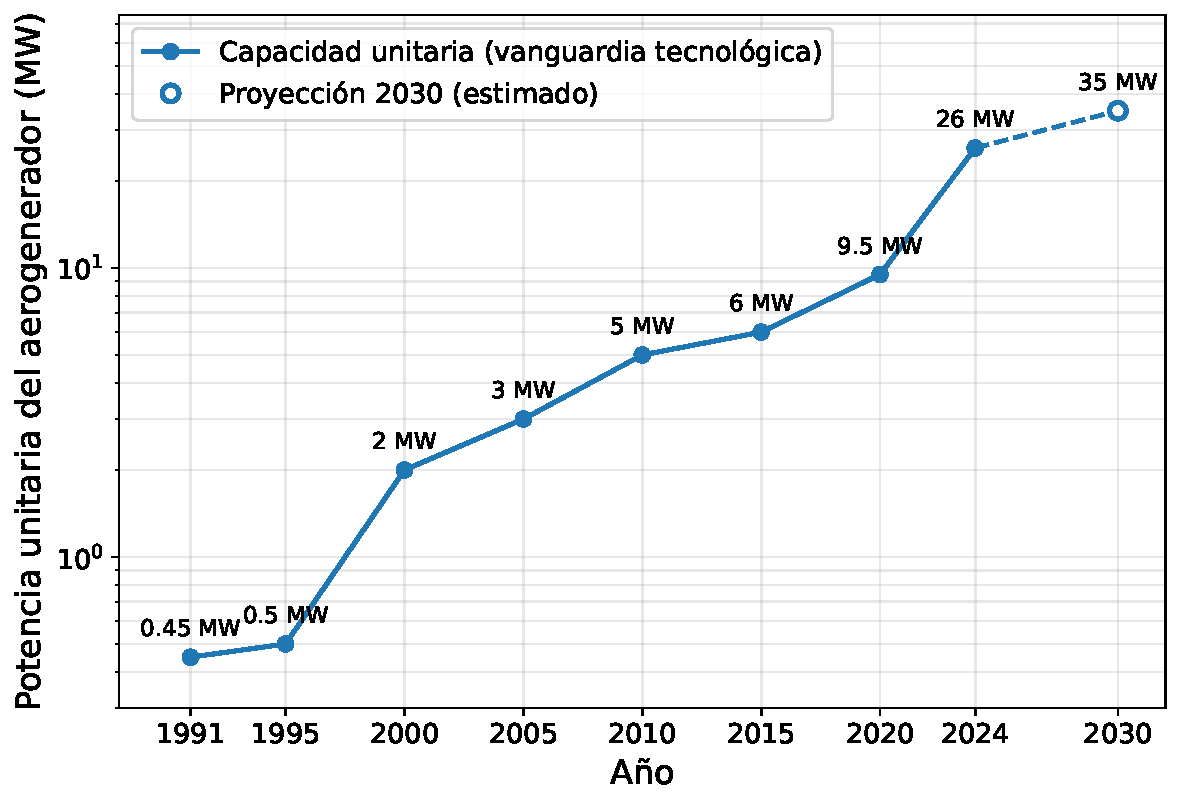
\includegraphics[width=0.75\textwidth]{Figuras/Figuras Antecedentes/crecimiento_turbinas_offshore.pdf}
    \caption[Crecimiento de la potencia unitaria de aerogeneradores offshore, 1991--2030.]{Crecimiento de la potencia unitaria de aerogeneradores offshore, 1991--2030. Elaboración propia a partir de los datos de \textcite{GWEC2025}.}
    \label{fig:crecimiento_turbinas}
\end{figure}

La densidad de potencia no es el único criterio relevante: también importa con qué frecuencia el viento se mantiene dentro del rango en que la turbina opera con eficiencia, aspecto que recoge el factor de planta, definido como el cociente entre la energía efectivamente generada en un periodo y la que se obtendría operando de forma continua a potencia nominal durante ese mismo periodo. En tierra, la turbulencia introducida por el relieve y los obstáculos vuelve el viento más irregular y reduce este valor incluso en las mejores zonas: esa misma franja de Chile central, de mayor recurso eólico terrestre del país, alcanza en el mar factores de planta de entre $40\%$ y $60\%$, superando el $70\%$ hacia el extremo sur~\parencite{Mattar2017}. A escala global, la flota offshore opera con un factor de planta medio ponderado del $41\%$~\parencite{GWEC2025}, cifra que ha llevado a organismos como la Agencia Internacional de Energía a describir la eólica marina como una tecnología de base variable, capaz de complementar el perfil diario y estacional de la generación solar~\parencite{GWEC2025}.

Este crecimiento no ha estado acompañado de un desarrollo equivalente de las bases científicas del diseño. Un grupo internacional de investigadores en energía eólica sistematizó, en la iniciativa \textit{Grand Challenges}, las brechas de conocimiento del sector en tres ámbitos críticos: la atmósfera, la turbina, y la planta junto a su interacción con la red~\parencite{Veers2022}. El segundo de ellos es el que enmarca directamente el presente trabajo. \textcite{Veers2022} señalan que el aumento de tamaño y flexibilidad de las máquinas modernas ha desplazado el diseño fuera del dominio en que fueron establecidos sus supuestos y sus herramientas de modelación, y que la evidencia experimental a gran escala disponible resulta insuficiente para validar los modelos y materiales empleados. Los mismos autores advierten, además, que el avance logrado hasta ahora se ha sustentado en soluciones de ingeniería que rodean esas brechas, apoyadas más en la experiencia acumulada que en la comprensión fundamental de los fenómenos, enfoque que ya no basta para sostener el ritmo de innovación requerido.

Estas brechas se acentúan en el entorno marino. El aprovechamiento del recurso en aguas profundas obliga a instalar la turbina sobre una plataforma flotante en lugar de anclarla directamente al fondo marino, de modo que la estructura queda sometida de forma simultánea al viento, al oleaje y a las corrientes, condiciones que definen el clima marino del emplazamiento y que se encuentran escasamente caracterizadas en comparación con las terrestres~\parencite{Veers2022}. A ello se suma que las nuevas máquinas deben ser, al mismo tiempo, mayores y más livianas para aprovechar ese recurso con eficiencia~\parencite{Veers2022}. La combinación de palas esbeltas con el movimiento de la plataforma traslada el punto crítico del diseño desde el rendimiento aerodinámico hacia la integridad estructural de componentes sometidos a cargas cíclicas de gran amplitud~\parencite{Borg2015}, y es en esa intersección, la verificación estructural de la pala bajo cargas aerodinámicas obtenidas conforme a la normativa vigente, donde se inscribe el presente trabajo.

\section{Potencial eólico offshore en Chile}

Chile posee un extenso borde costero y un potencial eólico marino que, según estudios del Banco Mundial~\parencite{BancoMundial2020}, supera los 957 GW, concentrado en la zona centro-sur y austral. El recurso es particularmente productivo hacia el extremo sur del país: en la franja entre los $45^\circ$ y $56^\circ$ S, que incluye la región de Magallanes, el factor de planta alcanza en gran medida valores superiores al $60\%$, llegando puntualmente al $70\%$~\parencite{Mattar2017}.

Este recurso se concentra mayoritariamente en zonas de alta profundidad donde las soluciones de cimentación fija no son viables: del potencial total, solo 131 GW corresponden a cimentación fija, mientras que la fracción más significativa, 826 GW, corresponde a las tecnologías flotantes, como se observa en la Figura~\ref{fig:potencial_offshore}~\parencite{BancoMundial2020}. Esta diferencia de escala sitúa a las plataformas flotantes como una alternativa viable para el aprovechamiento del recurso en el contexto nacional.

\begin{figure}[h]
    \centering
    %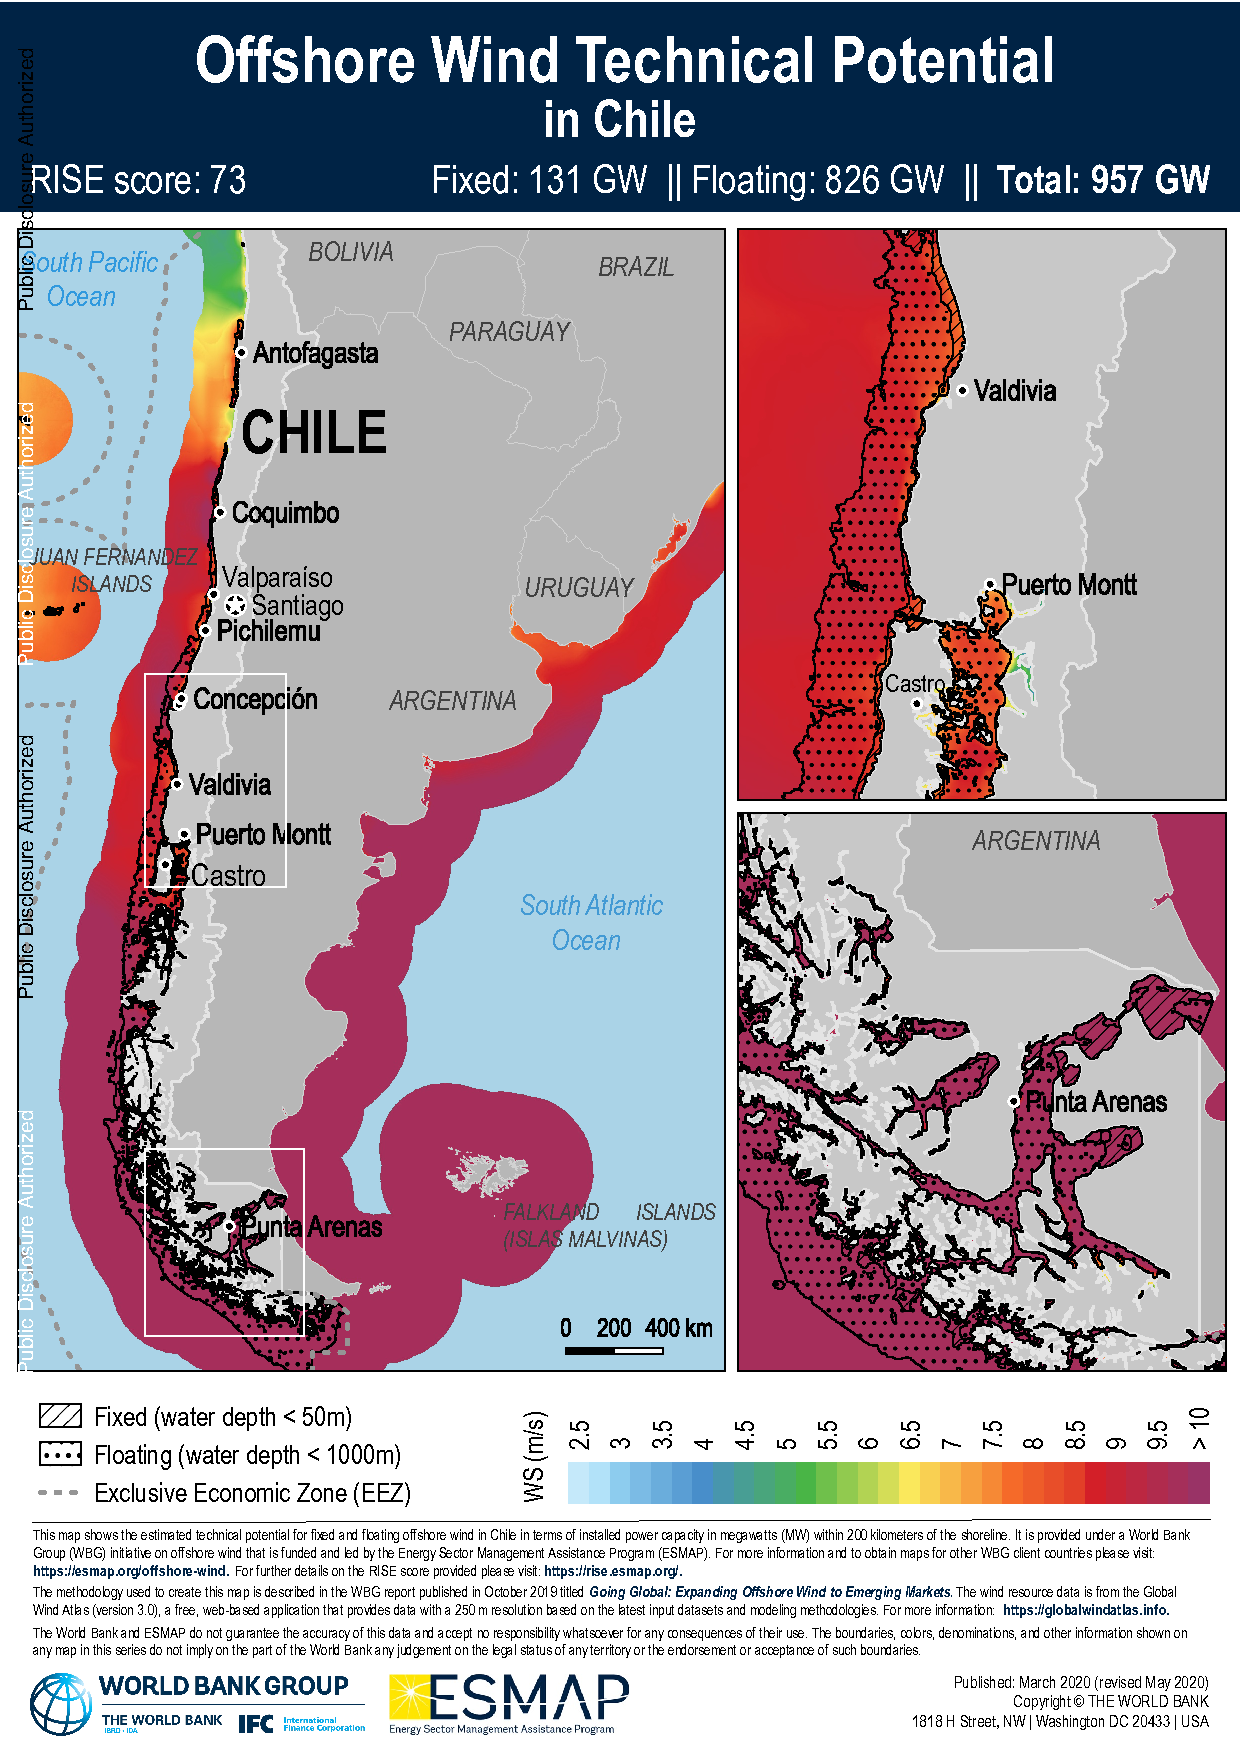
\includegraphics[width=0.75\textwidth]{Figuras/Technical-Potential-for-Offshore-Wind-in-Chile-Map.pdf}
    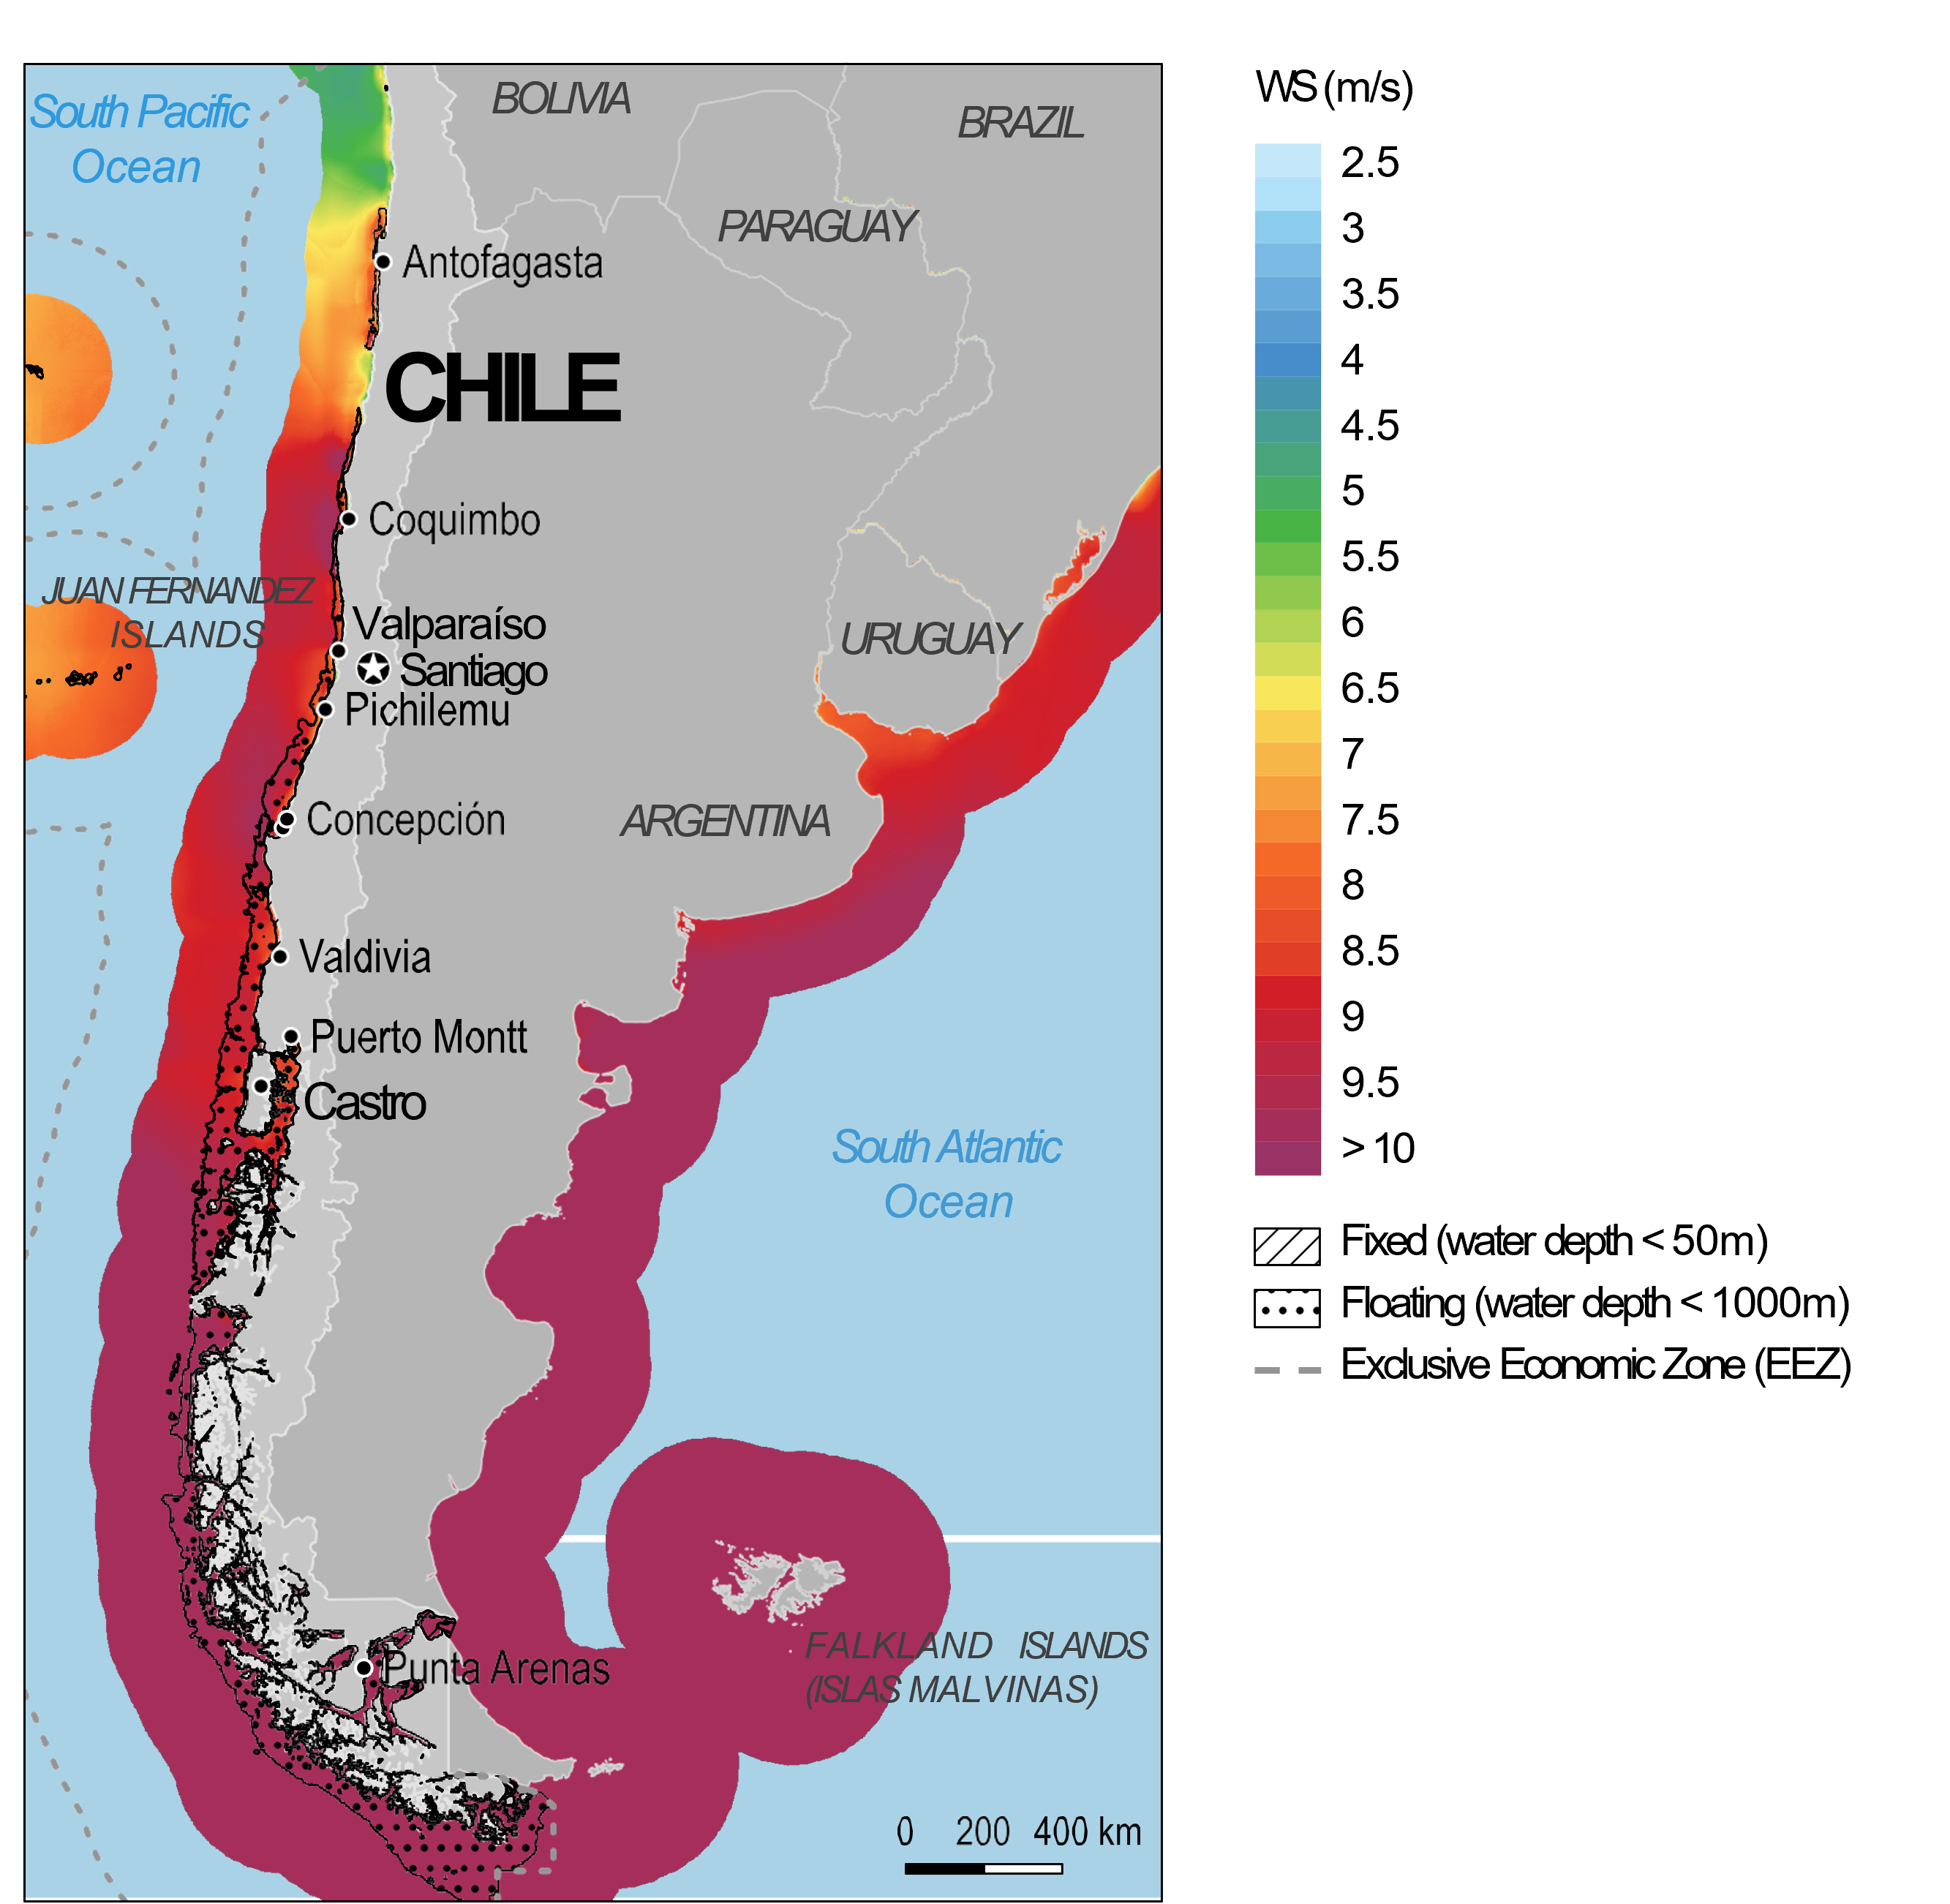
\includegraphics[width=0.75\textwidth]{Figuras/wind map.png}
    \caption[Modificado de potencial técnico de energía eólica marina en Chile.]{Modificado de potencial técnico de energía eólica marina en Chile~\parencite{BancoMundial2020}. La escala de color (WS) indica la velocidad media del viento (\textit{wind speed}); la fuente no especifica la altura de referencia a la que está evaluada.}
    \label{fig:potencial_offshore}
\end{figure}

\section{Tecnología offshore}
\label{sec:tecnologia-flotante}

El emplazamiento en el mar somete a la turbina a solicitaciones ausentes en tierra: a las cargas aerodinámicas se suman las condiciones de mar, cuyo efecto sobre el dimensionamiento estructural y sobre el análisis de fatiga resulta determinante~\parencite{Tampier2024}. En el caso de las estructuras flotantes, además, el oleaje induce movimientos de la plataforma que modifican la velocidad relativa del viento incidente sobre las palas y generan cargas inerciales adicionales~\parencite{Borg2015}. Estos efectos distinguen el diseño estructural offshore del terrestre y justifican la caracterización del recurso eólico bajo condiciones de turbulencia normal que se desarrolla en las secciones siguientes.

\subsection{Tipos de estructuras de soporte}

Las estructuras de soporte empleadas en el mar se agrupan en dos familias según su vínculo con el lecho marino, y la profundidad del emplazamiento es el criterio que determina cuál resulta aplicable, como se aprecia en la Figura~\ref{fig:tipos_estructuras}. Las estructuras fijas, solución dominante en la industria actual, transmiten las cargas directamente al lecho marino: el monopilote (\textit{monopile}), un cilindro de acero hincado en el fondo, cubre profundidades de 0 a 30 m, y la estructura reticulada tipo \textit{jacket} extiende el rango hasta los 25 a 60 m a costa de una mayor complejidad de fabricación; más allá de los 50 m, el volumen de material y las operaciones de instalación las vuelven económicamente inviables~\parencite{Tampier2024}.

A partir de esa profundidad se recurre a estructuras flotantes, ancladas mediante un sistema de fondeo y clasificadas según el mecanismo que provee la rigidez restauradora necesaria para limitar su inclinación~\parencite{Borg2015}: las estabilizadas por lastre, tipo \textit{spar}, concentran masa en su extremo inferior para situar el centro de gravedad muy por debajo del centro de la parte sumergida y operan desde los 120 m de profundidad; las estabilizadas por área de flotación, semisumergible o barcaza (\textit{barge}), obtienen el momento restaurador de la distribución horizontal de sus columnas o de su superficie de flotación y operan desde los 50 m; y las estabilizadas por fondeo, de piernas tensionadas (\textit{tension leg platform}), obtienen su rigidez de tirantes verticales pretensados anclados al fondo, que restringen fuertemente los movimientos verticales del conjunto~\parencite{Tampier2024,Borg2015}. Se estima que estos dispositivos podrán instalarse en profundidades de hasta 800 a 1\,000 m, si bien a la fecha el proyecto emplazado a mayor profundidad alcanza los 300 m~\parencite{Tampier2024}.

\begin{figure}[H]
    \centering
    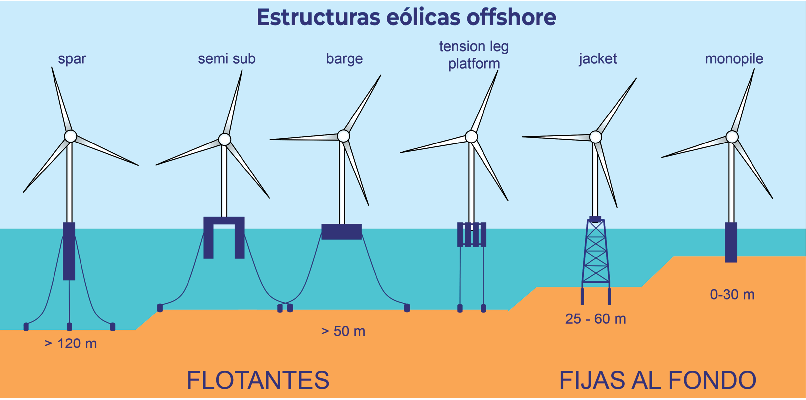
\includegraphics[width=0.85\textwidth]{Figuras/Figuras Antecedentes/estructuras_offshore.pdf}
    \caption[Estructuras eólicas offshore y profundidades típicas de instalación.]{Estructuras eólicas offshore y profundidades típicas de instalación~\parencite{Tampier2024}.}
    \label{fig:tipos_estructuras}
\end{figure}

\subsection{Retos del entorno flotante}
\label{sec:retos-flotante}

Mientras una torre terrestre se encuentra empotrada en el suelo, una plataforma flotante conserva seis grados de libertad de cuerpo rígido, definidos respecto de un sistema de coordenadas solidario a la estructura: tres desplazamientos, denominados \textit{surge} (longitudinal, en la dirección del viento), \textit{sway} (transversal) y \textit{heave} (vertical), y tres rotaciones, denominadas \textit{roll} (balanceo), \textit{pitch} (cabeceo) y \textit{yaw} (guiñada)~\parencite{Borg2015}. La Figura~\ref{fig:gdl_plataforma} ilustra esta convención.

\begin{figure}[H]
    \centering
    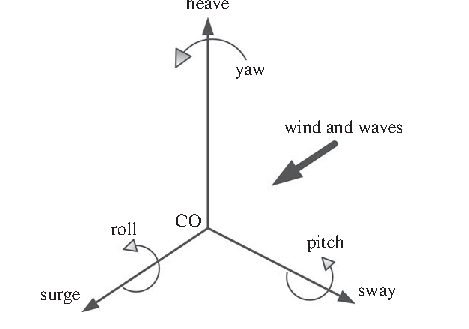
\includegraphics[width=0.55\textwidth]{Figuras/Figuras Antecedentes/gdl_plataforma.pdf}
    \caption[Grados de libertad de una plataforma eólica flotante.]{Grados de libertad de una plataforma eólica flotante respecto del centro de origen (CO)~\parencite{Borg2015}.}
    \label{fig:gdl_plataforma}
\end{figure}

De estos seis modos, el cabeceo es el que impone la restricción de diseño más severa, ya que el empuje aerodinámico del rotor actúa a gran altura sobre el centro de la parte sumergida y genera un momento de inclinación que la plataforma debe equilibrar. El diseño impone por ello un ángulo máximo de inclinación admisible, del cual se deriva la rigidez mínima que debe aportar la estructura de soporte: cuanto menor es el momento de inclinación que genera la turbina, menos costosa puede ser la subestructura~\parencite{Borg2015}.

A ello se suma un problema de acoplamiento dinámico. Las fuerzas aerodinámicas no solo desplazan la plataforma, sino que su carácter oscilatorio puede excitar sus modos propios de movimiento. \textcite{Borg2015} advierten que, en rotores de eje vertical de gran escala y baja velocidad de rotación, la frecuencia de paso de pala puede solaparse con el rango de frecuencias donde se concentra la energía del oleaje, condición que amplifica la respuesta del sistema y, con ella, la realimentación sobre la aerodinámica del rotor descrita al inicio de esta sección.

A estas restricciones se suma la orientación: una turbina de eje horizontal debe alinear activamente su rotor con la dirección del viento mediante un sistema de guiñada, que añade complejidad y masa en lo alto de la estructura, necesidad que desaparece en las configuraciones de eje vertical, insensibles a la dirección del viento incidente.

\subsection{Configuraciones de eje horizontal y de eje vertical}

Los aerogeneradores se clasifican según la orientación de su eje de rotación respecto del flujo incidente. En las turbinas eólicas de eje horizontal (HAWT, por sus siglas en inglés), el eje se dispone paralelo a la dirección del viento, de modo que el rotor debe orientarse activamente frente a él\glsunset{hawt}. Esta configuración domina las instalaciones de escala comercial, pero su despliegue está condicionado por el requerimiento de un flujo unidireccional y de baja turbulencia~\parencite{Essahraoui2026}.

En las turbinas eólicas de eje vertical (VAWT, por sus siglas en inglés), en cambio, el eje de rotación se dispone perpendicular a la componente horizontal del viento\glsunset{vawt}. De esta disposición se derivan sus propiedades características: la omnidireccionalidad, ya que el área barrida presenta la misma proyección con independencia de la dirección del viento, lo que elimina el sistema de guiñada y su hardware de control asociado; un centro de gravedad bajo, que simplifica las estructuras de soporte y las plataformas flotantes; una menor velocidad de punta; y una mayor tolerancia a la turbulencia~\parencite{Essahraoui2026}.

Dentro de la familia VAWT se distinguen a su vez las máquinas accionadas por arrastre, cuyo arquetipo es el rotor Savonius, y las accionadas por sustentación, correspondientes a las configuraciones Darrieus. Las primeras ofrecen un elevado torque de arranque y construcción simple, pero su coeficiente de potencia se limita a valores en torno a $0{,}25$; las segundas emplean perfiles alares y alcanzan coeficientes de potencia de $0{,}35$ a $0{,}45$ operando a relaciones de velocidad de punta mayores~\parencite{Essahraoui2026}.

Dentro de esas dos categorías, las configuraciones se diferencian por la forma y disposición de sus palas, según se representa en la Figura~\ref{fig:tipos_vawt}: el rotor Savonius, accionado por arrastre mediante palas acopadas; el H-Darrieus de pala recta; el Darrieus troposkeiano, de palas curvas que anulan la flexión bajo carga centrífuga; el Darrieus helicoidal, de palas retorcidas progresivamente en torno al eje para distribuir el torque a lo largo de la revolución; y las configuraciones híbridas, que acoplan un rotor Savonius interior a un Darrieus exterior para aprovechar su torque de arranque~\parencite{Essahraoui2026}.

\begin{figure}[H]
    \centering
    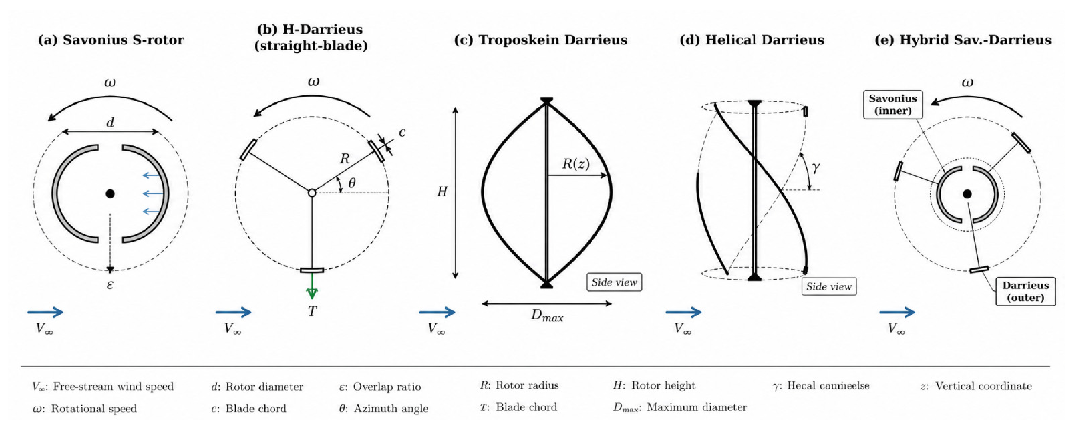
\includegraphics[width=\textwidth]{Figuras/Figuras Antecedentes/tipos_vawt.pdf}
    \caption[Configuraciones principales de VAWT.]{Configuraciones principales de VAWT~\parencite{Essahraoui2026}.}
    \label{fig:tipos_vawt}
\end{figure}

De todas ellas, el presente trabajo aborda una turbina tipo H-rotor, variante de pala recta de la familia Darrieus, cuyo análisis aerodinámico y estructural constituye el objetivo de esta memoria. Por este motivo, los antecedentes que se presentan a continuación se enfocan en las características de esta familia de VAWT y en su aplicación a plataformas flotantes offshore.

Aplicadas al entorno flotante, estas propiedades se traducen en ventajas concretas frente a la configuración de eje horizontal. Las \gls{vawt} permiten ubicar componentes pesados, como el generador y el tren de potencia, a menor altura que en las \gls{hawt}, lo que reduce el momento de inclinación de la plataforma y, con ello, la rigidez mínima que debe aportar la estructura de soporte~\parencite{Borg2015}. \textcite{ennis2018} cuantifican esta ventaja para un rotor Darrieus de 5 MW: las plataformas resultantes son más pequeñas y menos costosas que las de una HAWT flotante equivalente, debido principalmente al menor centro de gravedad y a los menores momentos de inercia del conjunto, si bien el rotor de baja velocidad y alto torque exige un tren de potencia de mayor masa. La omnidireccionalidad del rotor añade una ventaja frente a los casos de carga normados: ante un cambio extremo de dirección del viento, su operación no se ve alterada de forma apreciable, mientras que una HAWT pasaría a trabajar bajo flujo sesgado, esto es, con el viento incidiendo oblicuamente sobre el plano del rotor~\parencite{Galinos2015,HAND2021}.

La Figura~\ref{fig:vawt_hrotor} muestra la configuración general de la turbina H-rotor empleada como referencia para los análisis desarrollados en los capítulos siguientes.

\begin{figure}[H]
    \centering
    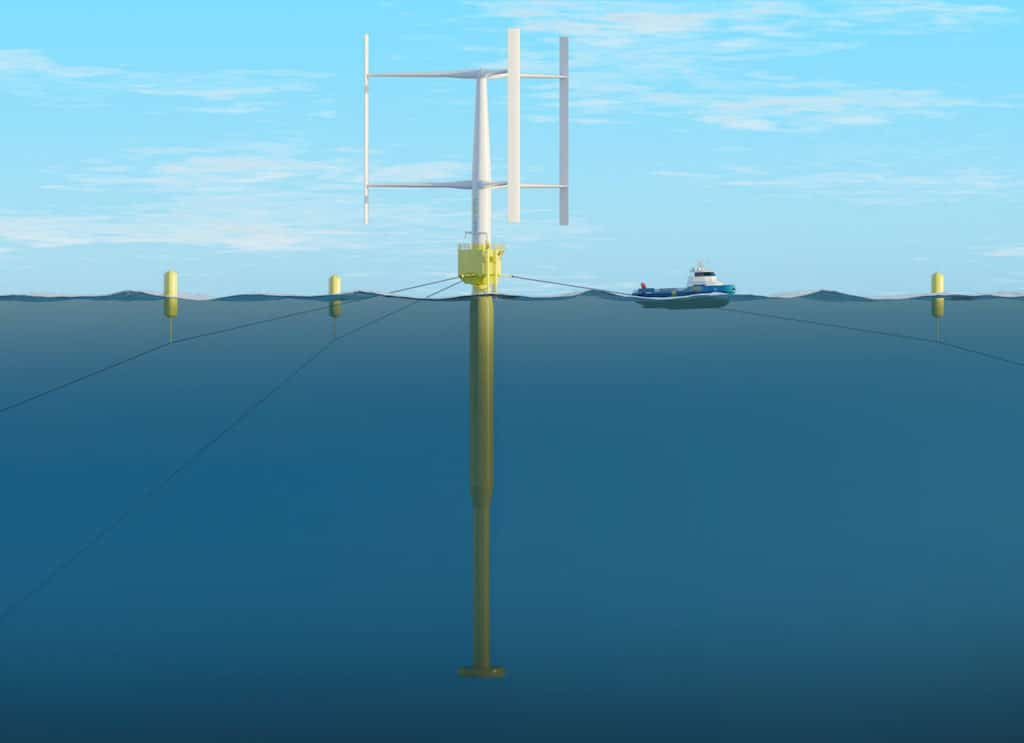
\includegraphics[width=0.6\textwidth]{Figuras/SeaTwirl_flotante.jpg}
    \caption[Configuración de aerogenerador de eje vertical tipo H-rotor.]{Configuración de aerogenerador de eje vertical tipo H-rotor empleada como caso de estudio~\parencite{SeaTwirl2026}.}
    \label{fig:vawt_hrotor}
\end{figure}

A diferencia de las turbinas de eje horizontal, cuyas cargas aerodinámicas presentan variaciones relativamente suaves durante la operación nominal, las VAWT en plataformas flotantes introducen desafíos de diseño propios: cada pala experimenta cambios periódicos en el ángulo de ataque y atraviesa repetidamente la estela generada por el propio rotor, mecanismos que dominan el campo de flujo y que los modelos cuasi-estacionarios no logran resolver~\parencite{Essahraoui2026}. En consecuencia, la determinación de las cargas de diseño requiere modelos aerodinámicos transitorios de mayor fidelidad~\parencite{Galinos2015}, constituyendo el punto de partida para analizar los principios aerodinámicos.

\section{Principios aerodinámicos de las VAWT}
\label{sec:aerodinamica}

\subsection{Geometría y partes del rotor}
\label{sec:geometria-rotor}

Un H-rotor está formado por un eje vertical, del cual se desprenden radialmente los brazos de soporte o \textit{struts}, y por un número $N$ de palas rectas de perfil alar montadas en el extremo de dichos brazos, dispuestas paralelas al eje de rotación. Esta disposición define las tres magnitudes geométricas que gobiernan el comportamiento del rotor, representadas en la Figura~\ref{fig:parametros_hrotor}:

\begin{itemize}
    \item El \textbf{radio del rotor} ($R$) es la distancia entre el eje de rotación y el plano medio de la pala. Corresponde al radio de la circunferencia que describe la pala al girar, y es la mitad del diámetro $D$ del rotor.
    \item La \textbf{altura de pala} ($H$) es la longitud de la pala medida en la dirección del eje de rotación.
    \item La \textbf{cuerda} ($c$) es la longitud de la sección transversal del perfil alar, medida sobre la línea recta que une su borde de ataque con su borde de fuga.
\end{itemize}

\begin{figure}[H]
    \centering
    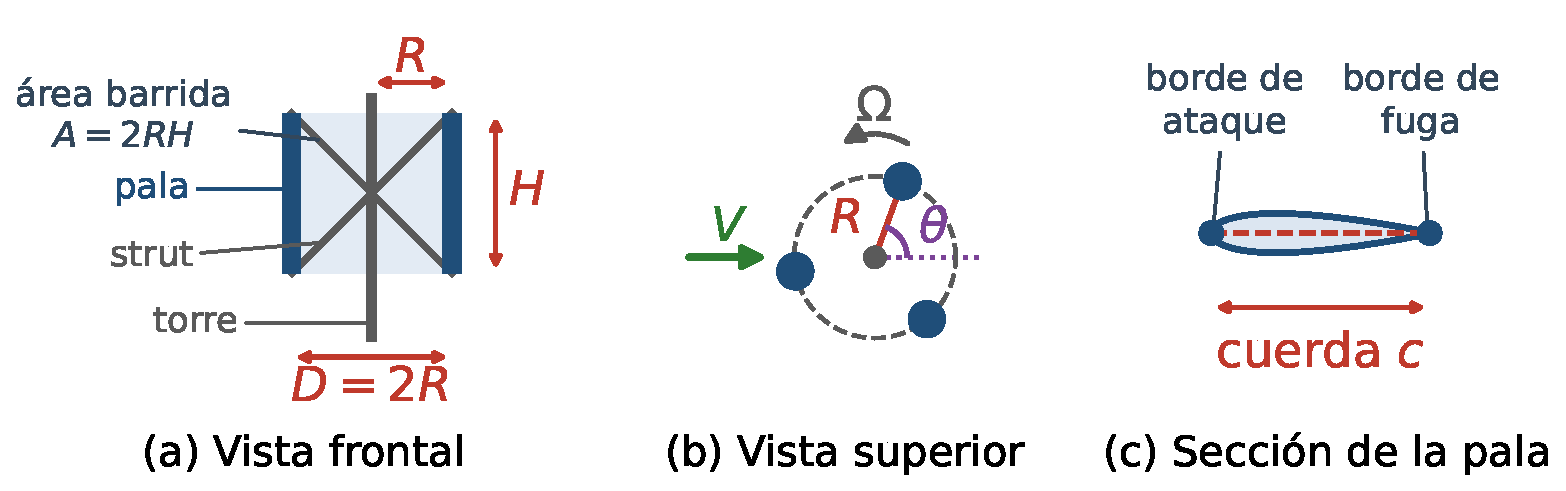
\includegraphics[width=\textwidth]{Figuras/Figuras Antecedentes/parametros_hrotor.pdf}
    \caption[Parámetros geométricos de un H-rotor.]{Parámetros geométricos de un H-rotor: radio $R$, diámetro $D$, altura de pala $H$, área barrida $A$, posición acimutal $\theta$ y cuerda $c$ de la sección. Elaboración propia.}
    \label{fig:parametros_hrotor}
\end{figure}

A diferencia de una \gls{hawt}, cuyo rotor barre un disco de área $\pi R^2$, el H-rotor barre la superficie lateral de un cilindro. El área proyectada frente al viento, que es la que interviene en los coeficientes adimensionales, corresponde por tanto al rectángulo de altura $H$ y ancho $D = 2R$, según la Ec.~\ref{eq:area_barrida}:

\begin{equation}
    A = 2RH
    \label{eq:area_barrida}
\end{equation}

Al girar, cada pala recorre una trayectoria circular sobre un plano horizontal. Su ubicación instantánea en dicha trayectoria se identifica mediante la \textbf{posición acimutal} ($\theta$), medida desde la dirección del viento incidente. La velocidad del viento se evalúa a la altura del centro del área barrida ($z_{hub}$), que en un H-rotor de palas rectas coincide con el punto medio de la pala, y la velocidad correspondiente a esa cota se denota $V_{hub}$. El subíndice conserva la notación de la norma IEC 61400-1, heredada de las \gls{hawt}, donde esa altura es la del buje que sostiene el rotor; en una VAWT no existe un elemento equivalente, por lo que la norma prescribe caracterizar las variables de viento a la altura del centro del área barrida~\parencite{IEC61400-1}.

La particularidad física del rotor de eje vertical reside en que la pala se desplaza alternadamente a favor y en contra del viento a lo largo de una misma revolución. En consecuencia, la velocidad relativa que percibe el perfil y el ángulo con que el flujo lo aborda varían de forma continua durante el giro, en contraste con una \gls{hawt}, donde ambas magnitudes permanecen aproximadamente constantes en operación nominal. De esta cinemática se derivan los parámetros que se definen a continuación.

\subsection{Parámetros adimensionales}

El rendimiento aerodinámico y las cargas sobre una turbina tipo H-rotor están gobernados por la interacción entre la velocidad del viento y la velocidad de rotación del sistema. Esta interacción se caracteriza mediante la relación de velocidad de punta (TSR, por sus siglas en inglés), que se define como la velocidad tangencial de la punta de la pala sobre la velocidad del viento, según la Ec.~\ref{eq:tsr}\glsunset{tsr}:

\begin{equation}
    \lambda = \frac{\Omega R}{V_{hub}}
    \label{eq:tsr}
\end{equation}

donde:
\begin{itemize}
    \item $\Omega$ es la velocidad angular de rotación (rad/s).
    \item $R$ es el radio del rotor (m).
    \item $V_{hub}$ es la velocidad del viento a la altura del centro del área barrida (m/s).
\end{itemize}

Para caracterizar el rendimiento del rotor se definen los coeficientes adimensionales de potencia ($C_p$) y de momento o torque ($C_m$), presentados en las Ecs.~\ref{eq:cp} y~\ref{eq:cm}, que expresan qué fracción de la potencia disponible en el flujo aprovecha la turbina y qué torque desarrolla, respectivamente:

\begin{equation}
    C_p = \frac{P}{\frac{1}{2}\rho A V_{hub}^3}
    \label{eq:cp}
\end{equation}

\begin{equation}
    C_m = \frac{M}{\frac{1}{2}\rho A R V_{hub}^2}
    \label{eq:cm}
\end{equation}

donde:
\begin{itemize}
    \item $P$ es la potencia mecánica generada.
    \item $M$ es el torque aerodinámico.
    \item $\rho$ es la densidad del fluido.
    \item $A = 2RH$ es el área barrida por el rotor, definida en la Ec.~\ref{eq:area_barrida}.
\end{itemize}

Ambos coeficientes no son independientes, sino que se relacionan a través de la relación de velocidad de punta mediante $C_p = \lambda C_m$~\parencite{Essahraoui2026}.

\subsection{Cinemática de la pala y ángulo de ataque}
\label{sec:cinematica}

La velocidad que percibe el perfil no es la del viento incidente, sino la \textbf{velocidad relativa} ($W$), resultante de componer la velocidad del viento con la velocidad tangencial de la pala. El \textbf{ángulo de ataque} ($\alpha$) es el ángulo formado entre la cuerda del perfil y la dirección de esa velocidad relativa, y es la variable que gobierna las fuerzas aerodinámicas sobre la pala. La Figura~\ref{fig:top_view} muestra el triángulo de velocidades que define ambas magnitudes en la vista superior del rotor.

\begin{figure}[H]
    \centering
    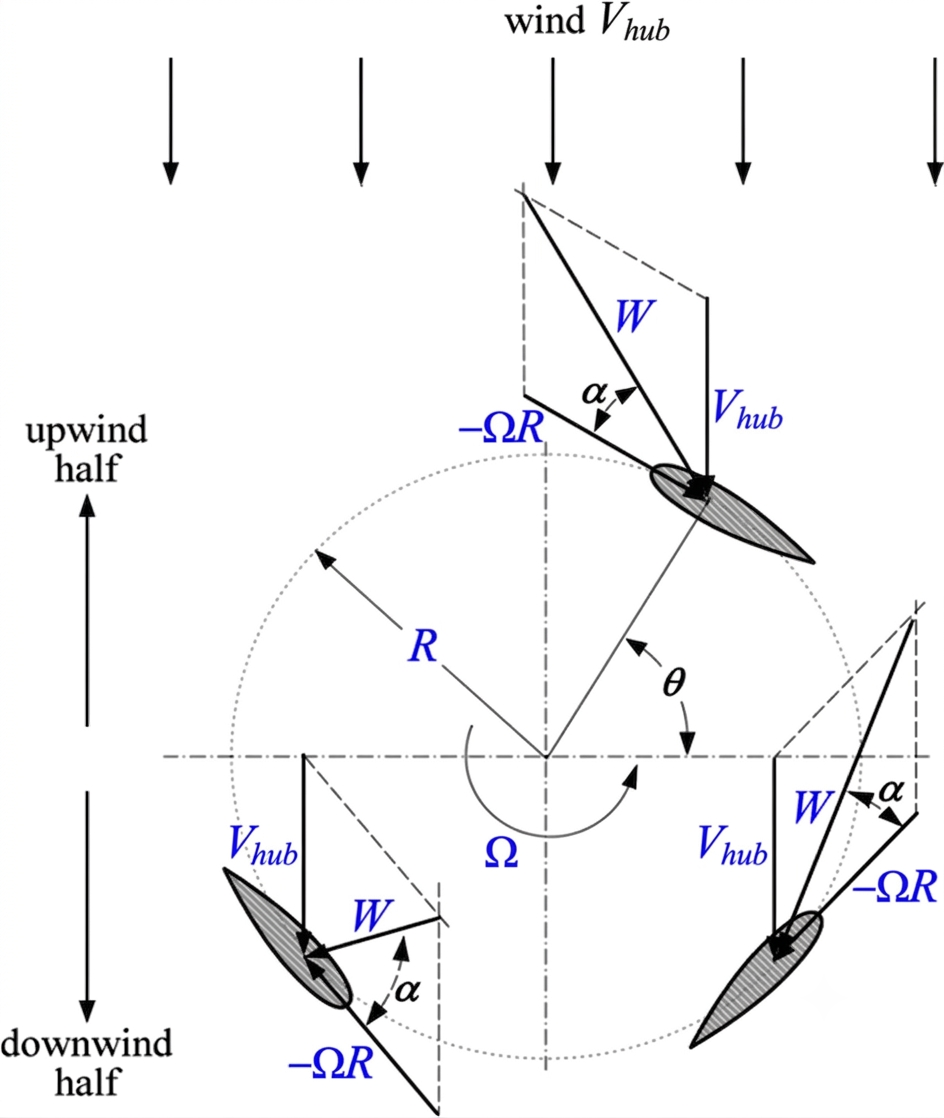
\includegraphics[width=0.5\textwidth]{Figuras/top_view_VAWT.png}
    \caption[Cinemática del H-rotor y triángulo de velocidades.]{Cinemática del H-rotor y triángulo de velocidades. El producto $\Omega R$ es la velocidad tangencial de la pala; el signo negativo indica que se compone en sentido opuesto a su avance. Modificado de \textcite{Tchakoua2015}.}
    \label{fig:top_view}
\end{figure}

En una \gls{hawt} el ángulo de ataque se mantiene relativamente constante en condiciones nominales. En un H-rotor, en cambio, la pala recorre posiciones a favor y en contra del viento dentro de una misma revolución, por lo que $\alpha$ experimenta una variación cíclica severa en función de la posición acimutal ($\theta$). Para un rotor de palas rectas, la cinemática básica define este ángulo según la Ec.~\ref{eq:alpha_theta}:

\begin{equation}
    \alpha(\theta) = \tan^{-1}\left(\frac{\sin\theta}{\lambda + \cos\theta}\right)
    \label{eq:alpha_theta}
\end{equation}

donde:
\begin{itemize}
    \item $\theta$ es la posición acimutal de la pala, medida desde la dirección del viento incidente.
    \item $\lambda$ es la relación de velocidad de punta definida en la Ec.~\ref{eq:tsr}.
\end{itemize}

Esta variación cíclica induce fluctuaciones en las cargas aerodinámicas durante cada revolución~\parencite{Bianchini2015,Borg2015}, fenómeno dominado por la pérdida dinámica que se describe en la Sección~\ref{sec:dynamicstall}.

\subsection{Solidez del rotor}
\label{sec:solidez}

La solidez ($\sigma$) relaciona la superficie total de pala con el área barrida. Para un H-rotor de $N$ palas de cuerda $c$ y radio $R$, se define según la Ec.~\ref{eq:solidez}:

\begin{equation}
\sigma = \frac{Nc}{R}
\label{eq:solidez}
\end{equation}

Este parámetro controla la posición del máximo de $C_p$ en función del TSR: rotores de baja solidez ($\sigma < 0{,}2$) operan a TSR elevados ($\lambda > 4$) con menor interferencia pala-estela, pero presentan pobre capacidad de autoarranque; rotores de alta solidez ($\sigma > 0{,}4$) alcanzan su máxima eficiencia a TSR bajos ($\lambda \approx 2\text{--}3$) y ofrecen mayor torque de arranque, a costa de una interacción pala-estela más intensa~\parencite{Essahraoui2026}.

Conviene advertir que la literatura emplea dos convenciones para esta magnitud. La adoptada en este trabajo, $\sigma = Nc/R$, es la de \textcite{Essahraoui2026}, mientras que otros autores la refieren al diámetro del rotor, $\sigma_d = Nc/d$~\parencite{Rezaeiha2018,Miller2021}, definición que para una misma geometría arroja la mitad del valor anterior. Cualquier contraste de solidez con datos de la literatura exige, por tanto, verificar previamente cuál de las dos definiciones emplea la fuente.

\subsection{Velocidad de punta y carga centrífuga}
\label{sec:vtip}

Sobre la pala en operación actúan tres tipos de carga: las aerodinámicas, las gravitatorias y las centrífugas, siendo estas dos últimas de naturaleza inercial y de carácter estacionario mientras la velocidad de rotación se mantenga constante~\parencite{Galinos2015}. Al describir la pala una trayectoria circular, la aceleración centrífuga a que queda sometida crece con el cuadrado de la velocidad de punta ($V_{tip} = \Omega R$), según la Ec.~\ref{eq:centrifugal_limit}:

\begin{equation}
    a_c = \Omega^2 R = \frac{V_{tip}^2}{R}
    \label{eq:centrifugal_limit}
\end{equation}

donde:
\begin{itemize}
    \item $a_c$ es la aceleración centrífuga en la punta de la pala, entendida como la fuerza inercial por unidad de masa que, en el marco de referencia solidario al rotor, actúa sobre la pala en dirección radial saliente. Su magnitud coincide con la de la aceleración centrípeta que describe el movimiento circular de la pala observado desde un marco fijo.
    \item $\Omega$ es la velocidad angular del rotor.
    \item $R$ es el radio del rotor.
\end{itemize}

El peso estructural de esta solicitación depende de la configuración del rotor. En un Darrieus de palas curvas la pala queda solicitada únicamente a tracción y sus tensiones de flexión radial resultan prácticamente nulas durante la operación, escenario particularmente favorable para un material compuesto~\parencite{Sutherland2012}. El H-rotor renuncia a esa condición a cambio de un radio constante: sus palas rectas, paralelas al eje de rotación, reciben la carga centrífuga en dirección perpendicular a su envergadura, que actúa como una carga transversal distribuida y las flecta entre sus puntos de unión a los struts, por lo que sus momentos flectores resultan mayores que en la configuración de palas curvas~\parencite{Mollerstrom2019}.

La velocidad de punta, por sí sola, no permite comparar máquinas de distinto tamaño. La Ec.~\ref{eq:centrifugal_limit} muestra que, para una misma velocidad de punta, la aceleración centrífuga es inversamente proporcional al radio: un rotor grande alcanza esa velocidad girando lentamente y con una solicitación moderada, mientras que uno pequeño debe girar mucho más rápido para lograrla y queda sometido a una solicitación mayor.

\subsection{Regímenes de operación y velocidad de rotación}
\label{sec:regimenes_operacion}

El coeficiente de potencia de un rotor depende de la relación de velocidad de punta (Ec.~\ref{eq:tsr}), de modo que aprovechar al máximo la energía disponible exige que la máquina permanezca en el $\lambda$ de mayor eficiencia. Como la velocidad del viento varía de forma continua, sostener esa condición obliga a que la velocidad de rotación la acompañe. La exigencia se acentúa en viento turbulento, condición en la que el \gls{tsr} óptimo de una \gls{vawt} de $200$~kW se desplaza respecto del que se obtiene en flujo uniforme~\parencite{Mollerstrom2016}.

La velocidad de rotación que sostiene un $\lambda$ dado para cada velocidad de viento se obtiene despejando la propia definición de la relación de velocidad de punta, según se desarrolla en la Sección~\ref{sec:criterio_rotacion}. Esa relación gobierna la operación por debajo de la velocidad de viento nominal, el régimen en que la turbina extrae la máxima energía disponible y en el que el $\lambda$ se mantiene constante en su valor de diseño.

Por encima de esa velocidad la relación deja de aplicarse, ya que continuar acelerando el rotor llevaría la velocidad de punta, y con ella la carga centrífuga de la Sección~\ref{sec:vtip}, más allá del límite admisible. La velocidad de rotación se mantiene entonces en su valor máximo y el \gls{tsr} decae a medida que el viento arrecia, con la consiguiente pérdida de coeficiente de potencia. La velocidad de viento que separa ambos regímenes queda determinada por la geometría del rotor y por ese límite de rotación, sin depender de ninguna magnitud ajena a ellos.

\subsection{Pérdida aerodinámica: del régimen estático al dinámico}
\label{sec:dynamicstall}

La pérdida aerodinámica, o \textit{stall}, es el fenómeno que fija el límite superior de la sustentación de un perfil y, en una \gls{vawt}, el que gobierna tanto la potencia extraída como las cargas cíclicas sobre la pala. Su descripción exige fijar previamente la nomenclatura del perfil alar, que se recoge en la Figura~\ref{fig:perfil_anatomia}.

\begin{figure}[H]
    \centering
    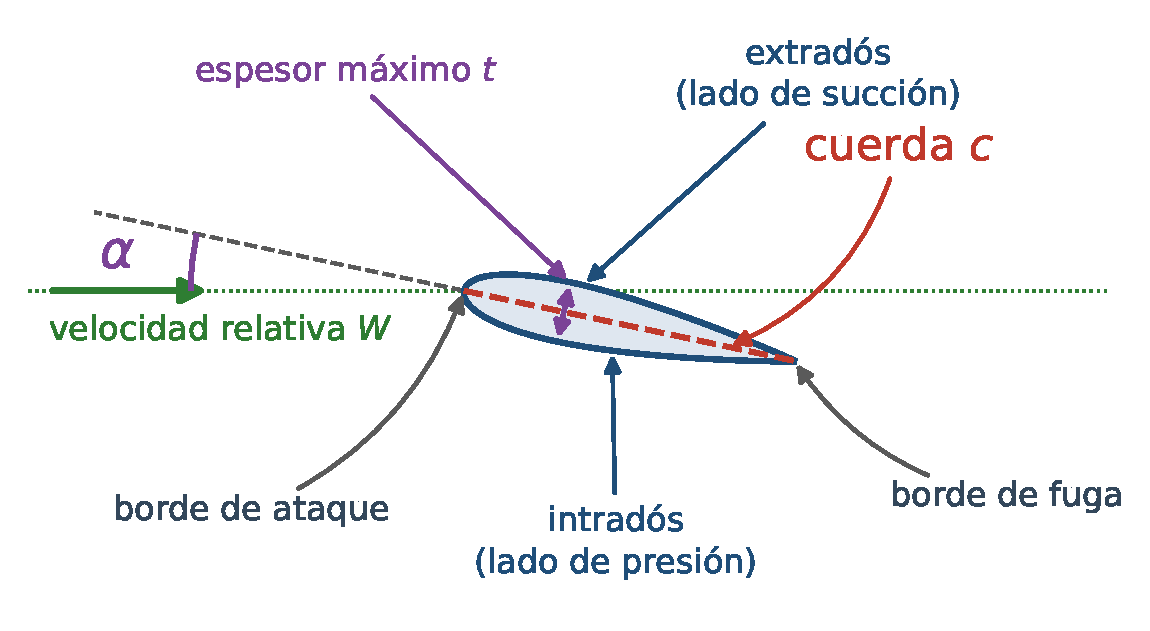
\includegraphics[width=0.82\textwidth]{Figuras/Figuras Antecedentes/perfil_anatomia.pdf}
    \caption{Nomenclatura del perfil alar y definición del ángulo de ataque.}
    \label{fig:perfil_anatomia}
\end{figure}

El borde de ataque es el extremo redondeado que enfrenta al flujo y el borde de fuga el extremo afilado opuesto. La recta que los une es la cuerda, de longitud $c$. La superficie superior, o extradós, es aquella sobre la cual el flujo se acelera y la presión disminuye, por lo que se denomina lado de succión; la inferior, o intradós, constituye el lado de presión. El espesor máximo $t$ caracteriza la esbeltez del perfil y, en la familia \gls{naca} de cuatro dígitos, se expresa como porcentaje de la cuerda. El ángulo de ataque $\alpha$ es el que forma la cuerda con la velocidad relativa $W$, según se definió en la Sección~\ref{sec:cinematica}.

La interacción entre el perfil y el flujo incidente produce una fuerza aerodinámica resultante que conviene descomponer respecto de la dirección de $W$: la sustentación es su componente perpendicular a $W$, y la resistencia (o arrastre), su componente paralela, en el sentido del flujo. Para comparar perfiles y condiciones de vuelo distintas, ambas se adimensionalizan dividiéndolas por la presión dinámica del flujo y el área de referencia, obteniéndose el coeficiente de sustentación $C_l$ y el coeficiente de resistencia $C_d$; de manera análoga se define el coeficiente de momento $C_m$, asociado al giro que la distribución de presiones induce sobre el perfil. Los tres dependen principalmente del ángulo de ataque $\alpha$ y, en menor medida, del número de Reynolds $Re$, razón entre las fuerzas inerciales y las viscosas del flujo, que caracteriza cuánto influye la viscosidad sobre su comportamiento. Las curvas de $C_l$, $C_d$ y $C_m$ en función de $\alpha$ para un $Re$ dado constituyen la polar aerodinámica del perfil, que se retoma con mayor detalle en la Sección~\ref{sec:polares}.

\subsubsection{Pérdida estática}

Sobre la superficie del perfil el aire no desliza libremente: la condición de adherencia impone velocidad nula en la pared, de modo que existe una región delgada, denominada capa límite, en la que la velocidad pasa de cero al valor del flujo exterior. Aguas abajo del punto de máxima succión el flujo debe recuperar presión, es decir, avanza contra un gradiente adverso de presión. Cuando ese gradiente es suficientemente intenso, el fluido de la capa límite, que ya ha perdido cantidad de movimiento por fricción viscosa, no logra continuar adherido y la capa límite se separa de la superficie.

La pérdida estática es la que se produce cuando el ángulo de ataque se incrementa lentamente. Al aumentar $\alpha$ crece la succión sobre el extradós y con ella el gradiente adverso, por lo que el punto de separación avanza progresivamente desde el borde de fuga hacia el de ataque, como ilustra la Figura~\ref{fig:stall_progresion}. Mientras el flujo permanece adherido, la sustentación crece de forma aproximadamente lineal con $\alpha$. Al alcanzarse el ángulo de pérdida estática $\alpha_{stall}$, la separación abarca ya una fracción sustancial del extradós: el coeficiente de sustentación alcanza su máximo $C_{l,max}$ y a partir de allí decae, mientras el coeficiente de arrastre aumenta con rapidez por efecto de la estela ancha que deja el perfil. La Figura~\ref{fig:stall_polar} recoge esta progresión sobre la polar del perfil \gls{naca}~0018.

\begin{figure}[H]
    \centering
    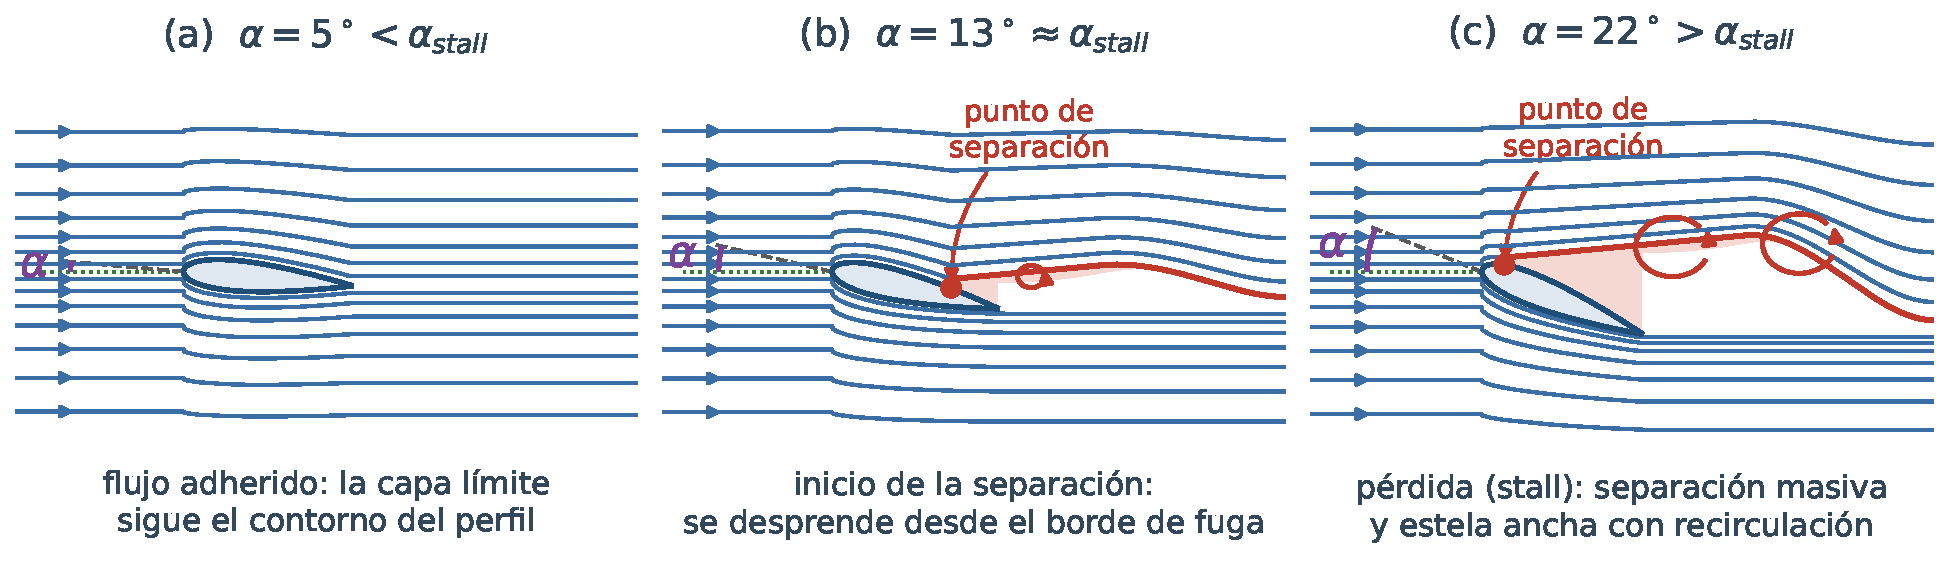
\includegraphics[width=\textwidth]{Figuras/Figuras Antecedentes/stall_progresion.pdf}
    \caption[Progresión de la separación de la capa límite con el ángulo de ataque.]{Progresión de la separación de la capa límite al aumentar el ángulo de ataque. La región sombreada indica la zona de flujo separado y las flechas circulares, la recirculación.}
    \label{fig:stall_progresion}
\end{figure}

\subsubsection{Pérdida dinámica}

Cuando el ángulo de ataque no varía lentamente sino con rapidez, como ocurre en la pala de una \gls{vawt} en cada revolución, la separación deja de seguir la secuencia estática. Durante la fase de aumento de $\alpha$ la capa límite permanece adherida más allá de $\alpha_{stall}$, retenida por la inercia del propio movimiento del flujo en las proximidades del borde de ataque, de modo que la sustentación continúa creciendo por encima de su máximo estático.

En esa condición se forma un vórtice de borde de ataque (LEV, por sus siglas en inglés)\glsunset{lev}, es decir, una concentración de vorticidad que nace del desprendimiento de la capa límite junto al borde de ataque y que permanece un tiempo sobre el extradós mientras crece. Al desplazarse sobre la superficie de succión induce una depresión adicional que se traduce en un exceso transitorio de sustentación, reportado en hasta un $50\%$ por encima del máximo estático~\parencite{Essahraoui2026}. Cuando el vórtice alcanza su tamaño límite se desprende y es arrastrado aguas abajo, momento en que la sustentación colapsa de forma abrupta, aparece flujo inverso sobre el extradós, esto es, una región donde el aire circula en sentido contrario al de la corriente principal, y el perfil entra en pérdida profunda.

Dado que la readherencia posterior del flujo ocurre a ángulos de ataque menores que aquel al que se produjo el desprendimiento, el ciclo de carga no es reversible: la curva $C_l$--$\alpha$ describe un lazo de histéresis, con sustentación superior a la estática durante el aumento de $\alpha$ e inferior durante su disminución~\parencite{Ferreira2009}. La carga real sobre la pala queda descrita por ese lazo y no por un valor único de $C_l$ para cada ángulo. La Figura~\ref{fig:stall_polar} contrasta ese lazo con la polar estática.

\begin{figure}[H]
    \centering
    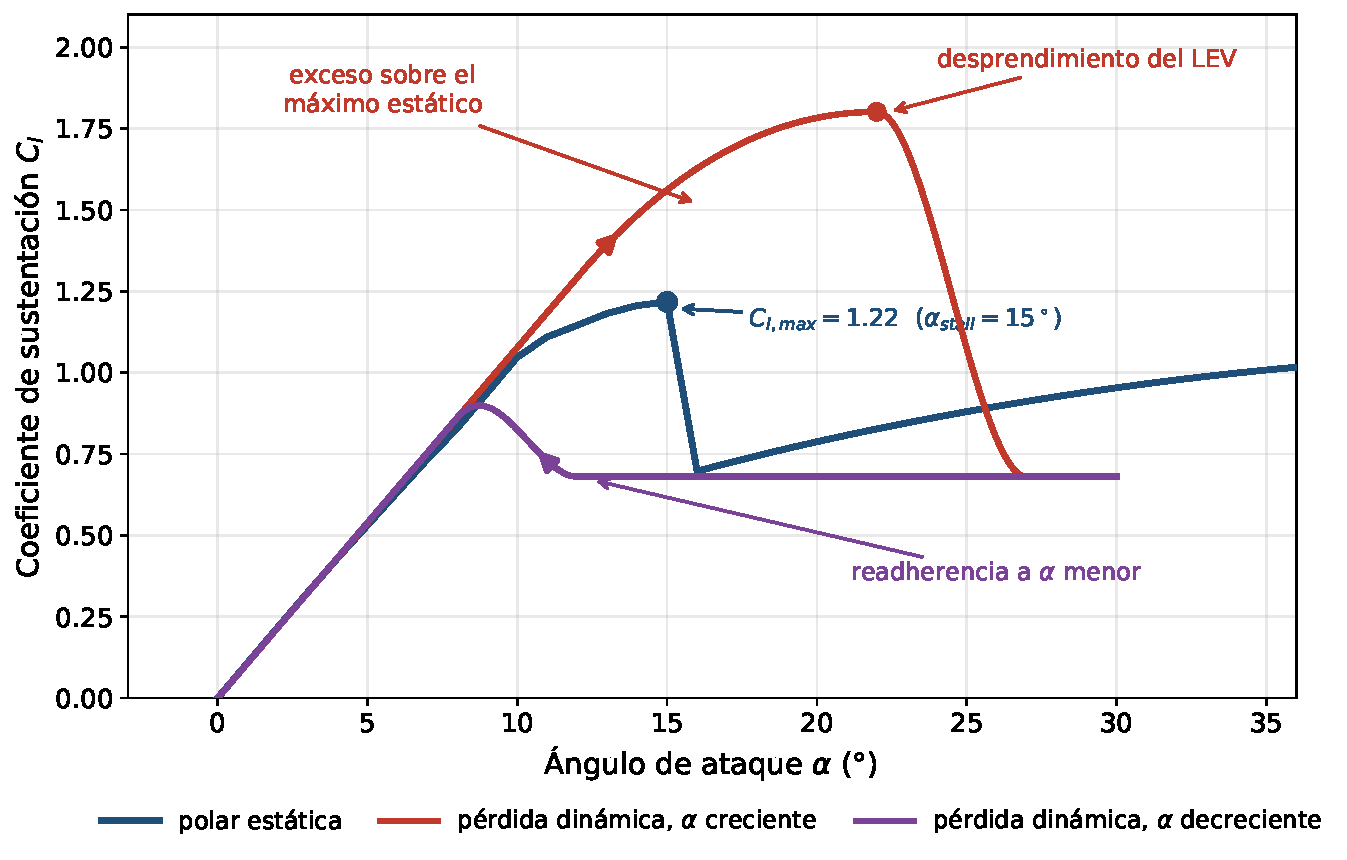
\includegraphics[width=0.8\textwidth]{Figuras/Figuras Antecedentes/stall_polar.pdf}
    \caption[Pérdida estática y dinámica del perfil NACA 0018.]{Pérdida estática y dinámica del perfil \gls{naca}~0018 a $Re = 1\times10^{6}$. La polar estática procede de las curvas calculadas para este trabajo; el lazo de histéresis es una representación cualitativa de la secuencia descrita en el texto, no una medición ni una simulación.}
    \label{fig:stall_polar}
\end{figure}

\subsubsection{Excursión del ángulo de ataque y su dependencia del TSR}

En un H-rotor la pala recorre una circunferencia mientras el viento sopla en una dirección fija, de manera que la posición acimutal $\theta$ determina la orientación relativa entre ambos. Se denomina semiciclo de barlovento a la mitad de la revolución en que la pala atraviesa el lado del rotor que enfrenta primero al viento, y semiciclo de sotavento a la mitad restante, en la cual la pala opera dentro de la estela generada por el propio rotor y encuentra, por tanto, un flujo ya frenado~\parencite{Essahraoui2026}.

El ángulo de ataque que percibe la pala queda determinado por la posición acimutal y por el \gls{tsr}, según la función $\alpha(\theta,\lambda)$ que expresa la Ec.~\ref{eq:alpha_theta}. Al derivar dicha expresión respecto de $\theta$ se obtiene que el extremo se alcanza en $\cos\theta = -1/\lambda$ y que su valor depende únicamente del \gls{tsr}, según la Ec.~\ref{eq:alpha_max}:

\begin{equation}
    \alpha_{max} = \arcsin\left(\frac{1}{\lambda}\right)
    \label{eq:alpha_max}
\end{equation}

La Ec.~\ref{eq:alpha_max} sintetiza el papel del \gls{tsr}: fijada la geometría, es la velocidad de rotación relativa a la del viento la que determina por sí sola la amplitud de la excursión angular. La Figura~\ref{fig:alpha_acimut} representa $\alpha(\theta)$ a lo largo de una revolución completa para tres valores de $\lambda$, junto con la banda en que el perfil se encuentra en pérdida.

\begin{figure}[H]
    \centering
    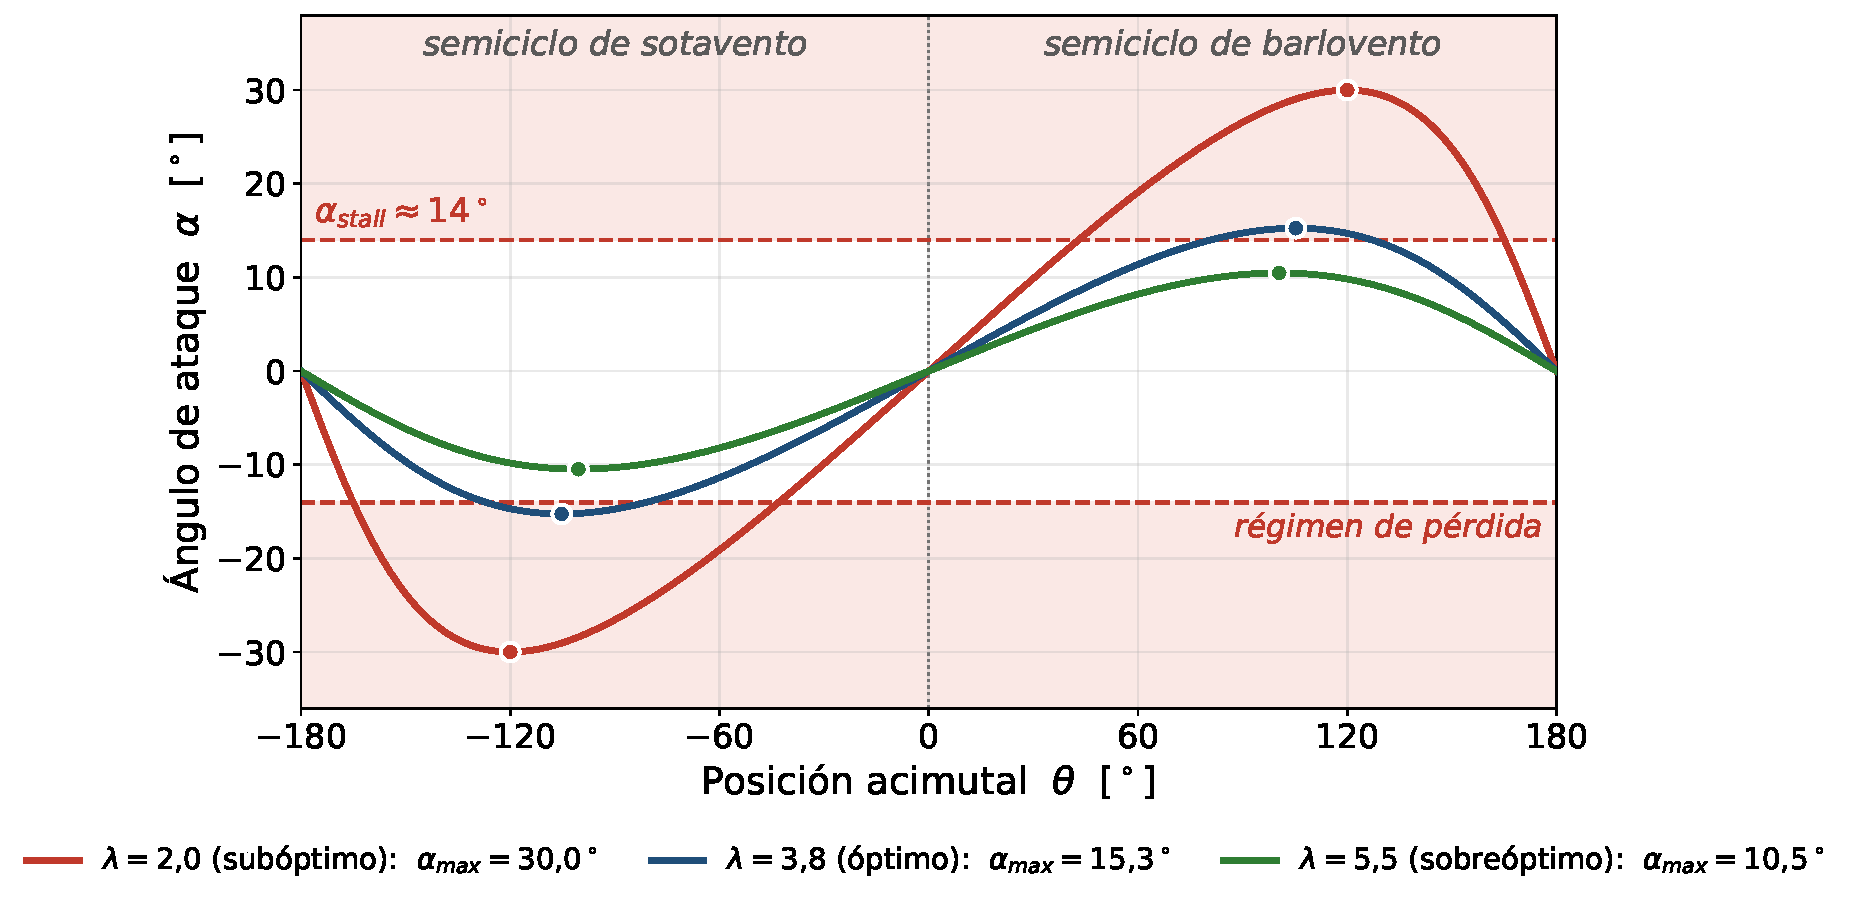
\includegraphics[width=0.92\textwidth]{Figuras/Figuras Antecedentes/alpha_acimut_tsr.pdf}
    \caption{Ángulo de ataque en función de la posición acimutal para tres \gls{tsr}.}
    \label{fig:alpha_acimut}
\end{figure}

La banda sombreada de la Figura~\ref{fig:alpha_acimut} corresponde al régimen de pérdida, delimitado por el ángulo de pérdida estática del perfil \gls{naca}~0018, que los ensayos en túnel de viento de \textcite{Bianchini2015} sitúan entre $14^\circ$ y $15^\circ$ para números de Reynolds de $1{,}5\times10^5$ a $3\times10^5$. Los puntos marcados sobre cada curva señalan los extremos que predice la Ec.~\ref{eq:alpha_max}. El contraste entre las tres ilustra el compromiso que fija el punto de operación: a $\lambda = 2$ la excursión alcanza $\alpha_{max} = 30^\circ$ y la pala atraviesa la banda de pérdida dos veces por revolución, una en cada semiciclo y con signos opuestos del ángulo de ataque; a $\lambda = 5{,}5$ el flujo permanece adherido durante todo el ciclo, pero el rotor opera lejos del máximo de sustentación y aumentan las pérdidas viscosas y la interferencia con la estela~\parencite{Essahraoui2026}. Entre ambos extremos, \textcite{Essahraoui2026} señalan que la restricción cinemática que fija el \gls{tsr} óptimo de una configuración es que la envolvente de ángulos de ataque permanezca acotada por el ángulo de pérdida estática.

Esta progresión cuenta con verificación experimental directa. \textcite{Ferreira2009} visualizaron mediante velocimetría de imágenes de partículas (PIV, por sus siglas en inglés)\glsunset{piv} el campo de flujo sobre la pala de un rotor Darrieus para $\lambda = 2$, $3$ y $4$: a $\lambda = 2$ registraron la formación del vórtice de borde de ataque, su desprendimiento y su posterior interacción con la pala en el semiciclo de sotavento, fenómenos que se atenúan a $\lambda = 3$ y desaparecen a $\lambda = 4$, donde los ángulos de ataque alcanzados ya no bastan para producir el enrollamiento. El máximo desarrollo del vórtice se observó, además, en la posición acimutal que predice la Ec.~\ref{eq:alpha_max}.

\subsubsection{Consecuencias sobre las cargas y la fatiga}

El efecto de esta cinemática sobre las cargas es doble. En primer lugar, el torque no es constante a lo largo de la revolución: en el semiciclo de barlovento la pala produce el pico principal de fuerza tangencial mientras $\alpha(\theta)$ se mantiene por debajo del ángulo de pérdida, en tanto que en el de sotavento, al operar sobre el flujo ya frenado por el propio rotor, genera un pico secundario de menor magnitud~\parencite{Essahraoui2026}. Con $N$ palas igualmente espaciadas el torque resultante oscila $N$ veces por revolución. Para configuraciones de dos y tres palas con flujo adherido, el cociente entre la variación pico a pico del torque y su valor medio se sitúa entre $0{,}5$ y $1{,}5$, y aumenta de forma pronunciada cuando aparece la pérdida dinámica, condición en que la forma de onda del torque se vuelve marcadamente no sinusoidal~\parencite{Essahraoui2026}.

En segundo lugar, y con consecuencias directas sobre el objeto de este trabajo, la pala queda sometida a un régimen de carga intrínsecamente cíclico. \textcite{Mollerstrom2019} constatan que los problemas de fatiga han sido recurrentes en los proyectos de \gls{vawt} documentados, y lo atribuyen a que la dirección de las fuerzas aerodinámicas sobre la pala cambia de manera continua durante cada revolución, lo que somete al material a tensiones cíclicas de gran amplitud y, dado que cada revolución aporta un ciclo, a recuentos de ciclos muy elevados a lo largo de la vida útil. Añaden que la operación a \gls{tsr} bajo, que en una turbina de paso fijo es la que corresponde a las velocidades de viento altas, introduce además la pérdida dinámica y vuelve aún más brusca la variación de las cargas, y precisan que una \gls{hawt} experimenta también tensiones cíclicas, pero en menor medida, pues con viento estable y baja turbulencia la fuerza aerodinámica dominante se mantiene relativamente constante.

Este historial admite, no obstante, una precisión importante. En la retrospectiva del programa de \gls{vawt} de los Laboratorios Nacionales Sandia, \textcite{Sutherland2012} atribuyen las fallas por fatiga de las décadas de 1970 a 1990 al empleo de palas extruidas en aluminio 6063-T5, material de pobres propiedades frente a la fatiga, y no al concepto en sí: sostienen que las \gls{vawt} no son intrínsecamente más propensas a la fatiga que las \gls{hawt}, y que con el conocimiento actual de las cargas es posible diseñar palas que las resistan de manera fiable. La exigencia, en cambio, se mantiene en toda su magnitud, ya que la pala debe soportar del orden de $10^9$ ciclos a lo largo de su vida de diseño, recuento para el cual las bases de datos de fatiga de los materiales siguen resultando escasas.

De ahí que la verificación de una pala de H-rotor no pueda limitarse a la resistencia última frente a la carga extrema, sino que deba incorporar la acumulación de daño por fatiga a lo largo de la vida de diseño, exigencia que la norma recoge mediante el \gls{fls} y que se aborda en la Sección~\ref{sec:analisis-estructural}.
\section{Referencias de contraste para el rotor en estudio}
\label{sec:referencias-contraste}

Las magnitudes definidas en la sección anterior permiten describir un rotor, pero no juzgar si los valores obtenidos para él son razonables. Esta sección reúne las referencias empíricas con que se contrastan los resultados del Capítulo~4: los rangos operacionales documentados para cada configuración de VAWT, los parámetros de máquinas H-rotor efectivamente construidas de escala comparable al caso de estudio, y los criterios con que pueden compararse rotores de distinto tamaño.

\subsection{Rangos operacionales por configuración}
\label{sec:configuraciones-vawt}


La Tabla~\ref{tab:tabla_vawt} resume los valores característicos de las familias de VAWT presentadas en la Figura~\ref{fig:tipos_vawt}. Su utilidad en este trabajo es servir de referencia de contraste: los valores de $C_{p,max}$ y de TSR obtenidos en el Capítulo 4 para la turbina en estudio deben situarse dentro del rango documentado para la columna H-Darrieus.

\begin{table}[H]
    \centering
    \caption[Parámetros característicos de las principales configuraciones de VAWT.]{Parámetros característicos de las principales configuraciones de VAWT~\parencite{Essahraoui2026}.}
    \label{tab:tabla_vawt}
    \begin{tabular}{lccccc}
        \hline
        \textbf{Parámetro} & \textbf{Savonius} & \textbf{H-Darrieus} & \textbf{Troposkein} & \textbf{Helical} & \textbf{Híbrido}\\
        \hline
        $\lambda$ típico & $0{,}7\text{--}1{,}5$ & $2\text{--}5$ & $2{,}5\text{--}5$ & $2{,}5\text{--}5$ & $1\text{--}3$\\
        $\sigma$ & --- & $0{,}15\text{--}0{,}45$ & $0{,}15\text{--}0{,}40$ & $0{,}20\text{--}0{,}40$ & $0{,}25\text{--}0{,}50$\\
        $C_{p,max}$ & $0{,}15\text{--}0{,}25$ & $0{,}35\text{--}0{,}42$ & $0{,}35\text{--}0{,}45$ & $0{,}30\text{--}0{,}40$ & $0{,}25\text{--}0{,}35$\\
        \hline
        \multicolumn{6}{p{0.95\textwidth}}{\footnotesize La misma fuente reporta $C_{p,max}$ de hasta $0{,}45$ para configuraciones H-Darrieus optimizadas.}
    \end{tabular}
\end{table}

\subsection{Turbinas H-rotor de referencia}
\label{sec:turbinas_referencia}

La Tabla~\ref{tab:hrotor_rpm} resume los parámetros de algunos de los H-rotor tripala de escala comparable construidos a la fecha.

\begin{table}[H]
    \centering
    \caption[Parámetros de turbinas H-rotor tripala de escala comparable.]{Parámetros de turbinas H-rotor tripala de escala comparable. Modificado de \textcite{Mollerstrom2019}.}
    \label{tab:hrotor_rpm}
    \begin{tabular}{lccccc}
        \hline
        \textbf{Turbina} & \textbf{D (m)} & \textbf{A (m$^2$)} & \textbf{Potencia nominal} & \textbf{$P/A$ (W/m$^2$)} & \textbf{Material de palas}\\
        \hline
        T1-turbine & 26{,}0 & 624 & 200 kW @ 12 m/s & 321 & Fibra de vidrio \\
        ANew-M1    & 24{,}0 & 360 & 200 kW @ 12 m/s & 556 & Vidrio y carbono \\
        Skwid      & 24{,}0 & 850\textsuperscript{*} & 500 kW @ 13 m/s & 588 & --- \\
        \hline
        \multicolumn{6}{p{0.92\textwidth}}{\footnotesize $P/A$: potencia específica. \textsuperscript{*}Área estimada en la fuente.}
    \end{tabular}
\end{table}

Las tres máquinas de la Tabla~\ref{tab:hrotor_rpm} son H-rotor tripala de eje vertical con generador de accionamiento directo y velocidad variable. La T1-turbine es un prototipo terrestre instalado en Falkenberg, Suecia (2010), con palas de fibra de vidrio; la ANew-M1, un prototipo terrestre emplazado cerca de Cracovia, Polonia (2015), con torre de acero y palas de fibra de vidrio y carbono; y la Skwid, un prototipo flotante offshore desarrollado en Japón (2013), que acoplaba el H-rotor a un rotor Savonius sumergido para el aprovechamiento de corrientes~\parencite{Mollerstrom2019}.

Al tratarse de máquinas efectivamente construidas y operadas, sus parámetros provienen de la experiencia y no de un ejercicio de diseño, y como comparten con el caso de estudio la configuración H-rotor tripala y un orden de magnitud equivalente en diámetro y área barrida, sus rangos de velocidad de rotación, \gls{tsr} y potencia específica delimitan el espacio de valores razonable para una máquina de esta familia y escala. De ellas, la T1-turbine es la que cuenta con más parámetros operacionales documentados en la literatura revisada, resumidos en la Tabla~\ref{tab:t1_params}.

\begin{table}[H]
    \centering
    \caption[Parámetros operacionales de la T1-turbine.]{Parámetros operacionales de la T1-turbine. Fuentes: (1)~\textcite{Mollerstrom2019}, (2)~\textcite{Mollerstrom2017}, (3)~\textcite{Mollerstrom2016}.}
    \label{tab:t1_params}
    \begin{tabular}{l c c}
        \hline
        \textbf{Parámetro} & \textbf{Valor} & \textbf{Fuente}\\
        \hline
        Diámetro del rotor            & $26$ m         & (1), (2)\\
        Longitud de pala              & $24$ m         & (1), (2)\\
        Velocidad de viento nominal   & $12$ m/s       & (1), (3)\\
        Velocidad de corte            & $25$ m/s       & (2), (3)\\
        \gls{tsr} objetivo            & $3{,}8$        & (2), (3)\\
        Velocidad de rotación         & $16$--$33$ rpm & (2), (3)\\
        \hline
    \end{tabular}
\end{table}

La Figura~\ref{fig:t1_turbine} muestra la T1-turbine instalada en Falkenberg. Se trata de un H-rotor de palas rectas, con tres palas de perfil alar dispuestas paralelas al eje de rotación y unidas a este mediante struts, de acuerdo con la configuración descrita en la Sección~\ref{sec:geometria-rotor}. Los tensores visibles en la imagen no forman parte del diseño original y fueron incorporados con posterioridad.

\begin{figure}[H]
    \centering
    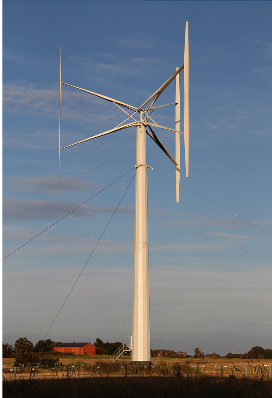
\includegraphics[width=0.42\textwidth]{Figuras/Figuras Antecedentes/t1_turbine.pdf}
    \caption[T1-turbine de 200 kW en Falkenberg, Suecia.]{T1-turbine de 200 kW en Falkenberg, Suecia~\parencite{Mollerstrom2019}.}
    \label{fig:t1_turbine}
\end{figure}

\subsection{Parámetros de comparación y velocidad de rotación de diseño}
\label{sec:criterio_rotacion}

La aceleración centrífuga de la Sección~\ref{sec:vtip} permite contrastar la severidad estructural de dos rotores de distinto radio, pero nada dice sobre su desempeño aerodinámico, comparación que se apoya en magnitudes normalizadas antes que en valores absolutos. Para las VAWT, \textcite{Essahraoui2026} identifican, junto al principio de operación, cuatro parámetros de gobierno para contrastar configuraciones: la relación de velocidad de punta $\lambda$, la solidez $\sigma$, el número de Reynolds basado en la cuerda $Re_c$ y el coeficiente de potencia máximo $C_{p,max}$, todos ellos definidos en este capítulo. A ellos se suma la potencia específica, cociente entre la potencia nominal y el área barrida, que permite comparar el dimensionamiento de máquinas efectivamente construidas: \textcite{Mollerstrom2019} reporta valores de hasta $1\,000$~W/m$^2$ en las VAWT históricas, que privilegiaron la potencia instalada por sobre el área de rotor, frente a los $200$ a $500$~W/m$^2$ habituales en una HAWT moderna. La Tabla~\ref{tab:hrotor_rpm} recoge este parámetro para las máquinas allí reseñadas.

Despejada la relación de velocidad de punta (Ec.~\ref{eq:tsr}), se obtiene la velocidad de rotación que corresponde a un \gls{tsr} y a una velocidad de viento dados, según la Ec.~\ref{eq:omega_from_vtip}:

\begin{equation}
    \Omega = \frac{\lambda \, V}{R}
    \label{eq:omega_from_vtip}
\end{equation}

La expresión adquiere carácter de criterio al evaluarla con el \gls{tsr} de mayor eficiencia del rotor y la velocidad de viento nominal, pues la velocidad de rotación así obtenida sitúa a la máquina en su punto de operación más eficiente justo cuando alcanza su potencia nominal. Su utilidad como referencia se acredita de forma empírica: evaluada con el \gls{tsr} objetivo y la velocidad de viento nominal documentados para la T1-turbine, reproduce su velocidad de rotación máxima registrada (Tabla~\ref{tab:t1_params}). Que la velocidad así estimada resulte además estructuralmente admisible es un problema distinto, que depende del radio a través de la aceleración centrífuga.

\section{Emplazamiento y recurso eólico del caso de estudio}

El diseño de un aerogenerador no puede definirse de forma genérica: la norma IEC 61400-1~\parencite{IEC61400-1} condiciona las cargas de diseño a la clasificación del emplazamiento según su régimen de vientos, de modo que la ubicación geográfica, la distribución estadística de la velocidad del viento y la calidad de los datos meteorológicos disponibles determinan directamente las condiciones bajo las cuales debe verificarse la turbina.

\subsection{Sitio de instalación}
\label{sec:sitio_instalacion}

El emplazamiento considerado para este estudio se sitúa mar adentro frente a la Región de Los Lagos, en la costa sur de Chile, en las coordenadas $41{,}4723^\circ$ S y $73{,}9562^\circ$ O. Esta zona se caracteriza por la presencia de vientos intensos y persistentes provenientes del oeste, con una velocidad media anual de $8{,}16$ m/s a la altura del centro del área barrida y una clasificación de emplazamiento Clase II$_A$ según IEC 61400-1 (el número romano fija la clase por velocidad de referencia y la letra, la categoría de turbulencia, ambas detalladas más adelante en este capítulo). La profundidad del lecho marino en la zona supera los $50$ m, lo que descarta el uso de cimentaciones fijas y favorece las plataformas flotantes como única alternativa viable~\parencite{Mattar2017}. Es esa exigencia de calado la que lleva el emplazamiento mar adentro, sobre aguas abiertas. Los datos de viento provienen del explorador eólico del Ministerio de Energía de Chile~\parencite{ExploradorEolico2018}.

\subsection{Distribución de probabilidad del viento}
\label{sec:distribucion_viento}

De acuerdo con la norma IEC 61400-1, la variabilidad de la velocidad del viento se modela mediante funciones de distribución de probabilidad. La norma adopta la distribución de Rayleigh como modelo de referencia para las clases estándar (I, II y III), la cual constituye un caso particular de la distribución de Weibull con parámetro de forma $k = 2$~\parencite{ennis2018}. Para evaluaciones sitio-específicas con registros históricos, se emplea la distribución de Weibull completa, dada por la Ec.~\ref{eq:weibull_cdf}:

\begin{equation}
    P_W(V_0) = 1 - \exp\left[-\left(\frac{V_0}{c}\right)^k\right]
    \label{eq:weibull_cdf}
\end{equation}

donde $P_W(V_0)$ es la probabilidad de que la velocidad del viento sea igual o inferior a un valor de referencia $V_0$ (m/s), $c$ es el parámetro de escala (m/s), vinculado a la velocidad media del viento, y $k$ es el parámetro de forma (adimensional), que refleja la regularidad del recurso eólico~\parencite{IEC61400-1,ennis2018}.

El efecto de estos dos parámetros sobre la forma de la distribución se ilustra en la Figura~\ref{fig:weibull_zonas}. Un aumento del parámetro de escala $c$ desplaza la distribución hacia velocidades mayores, como se aprecia al comparar las clases IEC I, II y III (Figura~\ref{fig:weibull_zonas}a), cuyas velocidades medias de referencia se obtienen de $V_{ave} = 0{,}2\,V_{ref}$ (Ec.~\ref{eq:vave_vref}). El parámetro de forma $k$, en cambio, controla la dispersión en torno a esa media: valores bajos describen un régimen de vientos más irregular, con mayor probabilidad de calmas y de ráfagas intensas, mientras que valores altos la concentran en torno a la media y describen un régimen más estable (Figura~\ref{fig:weibull_zonas}b). La Tabla 1 de la IEC 61400-1 define las clases únicamente en términos de $V_{ref}$ e $I_{ref}$, de modo que la clase fija indirectamente el parámetro de escala $c$ a través de $V_{ave} = 0{,}2\,V_{ref}$, pero no hace lo propio con $k$, que en este trabajo se ajusta a partir del registro histórico del emplazamiento ($k = 2{,}09$, Sección~\ref{sec:recurso_eolico}), valor cercano al $k = 2$ del modelo de referencia.

\begin{figure}[H]
    \centering
    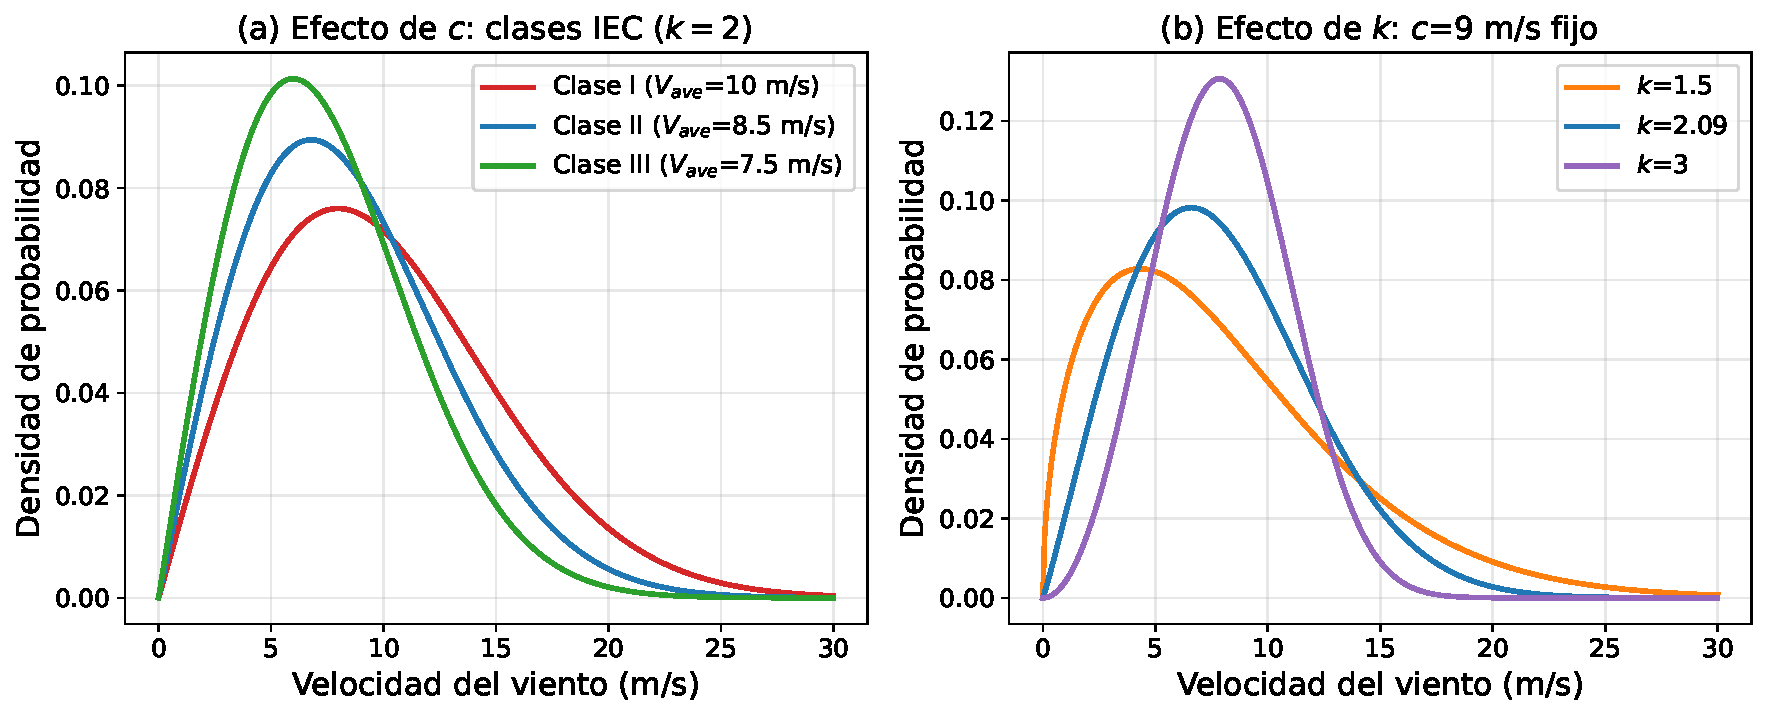
\includegraphics[width=\textwidth]{Figuras/Figuras Antecedentes/weibull_zonas.pdf}
    \caption{Efecto de los parámetros $c$ y $k$ de la distribución de Weibull.}
    \label{fig:weibull_zonas}
\end{figure}

\section{Marco normativo y condiciones de diseño}
\label{sec:marco-normativo}

La determinación de las cargas y la verificación estructural no dependen únicamente de modelos numéricos, sino también del cumplimiento de procedimientos establecidos por normas internacionales, que aseguran la integridad estructural ante condiciones ambientales extremas. El marco aplicable a este trabajo lo componen cuatro documentos de la serie IEC 61400, cada uno con un alcance distinto.

La norma IEC 61400-1 establece los requisitos generales de diseño y seguridad, y declara en su Sección 1 que se aplica a aerogeneradores de todos los tamaños, sin introducir restricción alguna respecto de la orientación del eje de rotación~\parencite{IEC61400-1}. La norma IEC 61400-3-1 extiende esos lineamientos al entorno marino de fundación fija y es la que prescribe las condiciones de viento sobre el mar que se emplean en este trabajo~\parencite{IEC61400-3-1}. La norma IEC 61400-3-2 aborda el caso de las estructuras flotantes, pertinente por la naturaleza del emplazamiento, si bien acota su alcance a plataformas no tripuladas con una única turbina de eje horizontal y advierte de forma expresa que las de eje vertical requieren consideraciones adicionales~\parencite{IEC61400-3-2}. Esa advertencia delimita con precisión el alcance de la presente verificación y se retoma al declarar sus limitaciones.

La norma IEC 61400-5, por último, es la específica de palas de aerogenerador y, por tanto, la directamente aplicable al objeto de este trabajo. Su Sección 1 declara que está destinada a las palas de todos los aerogeneradores y que la mayoría de los principios que recoge resultan aplicables a cualquier configuración de rotor, tamaño y material~\parencite{IEC61400-5}. Su pertinencia es doble, ya que además de los criterios de verificación estructural aporta un sistema de factores parciales de material más detallado que el de la IEC 61400-1 y una formulación de las cargas de pala que no presupone una geometría en voladizo, aspectos ambos que se desarrollan en las Secciones~\ref{sec:extrapolacion_teoria} y~\ref{sec:pandeo_teoria}.

\subsection{Parámetros de diseño y condiciones de carga}
\label{sec:condiciones_diseno}

Para garantizar la integridad estructural, la caracterización del viento según la norma IEC 61400-1 se organiza en el grupo de condiciones normales de operación, que definen el comportamiento recurrente del viento y los estados de carga de la estructura:

\textbf{Condiciones normales de viento (NWC, por sus siglas en inglés):} Incluyen el perfil de viento normal (NWP, por sus siglas en inglés), el cual describe la variación de la velocidad con la altura ($z$) mediante la ley de potencia de la Ec.~\ref{eq:nwp_ley_potencia}, con un exponente de cizalladura $\alpha_z$ que la norma IEC 61400-3-1 fija en $0{,}14$ para las condiciones normales de viento en emplazamientos marinos~\parencite{IEC61400-3-1}\glsunset{nwc}\glsunset{nwp}:

\begin{equation}
    V(z) = V_{hub} \left(\frac{z}{z_{hub}}\right)^{\alpha_z}
    \label{eq:nwp_ley_potencia}
\end{equation}

Asimismo, el modelo de turbulencia normal (NTM, por sus siglas en inglés)\glsunset{ntm} define la desviación estándar representativa de la turbulencia ($\sigma_{NTM}$) como el cuantil del $90\%$ de la desviación estándar de la velocidad para cada velocidad a la altura de referencia, y la expresa como una función lineal de esta última, según la Ec.~\ref{eq:ntm_sigma}:

\begin{equation}
    \sigma_{NTM} = I_{ref} \left(0{,}75 \, V_{hub} + b_{NTM}\right)
    \label{eq:ntm_sigma}
\end{equation}

donde $I_{ref}$ es la intensidad de turbulencia de referencia, parámetro adimensional que la norma tabula según la categoría de turbina ($0{,}16$ para la A, $0{,}14$ para la B y $0{,}12$ para la C) y que caracteriza la intensidad de las ráfagas esperada en el emplazamiento, y $b_{NTM}$ es el parámetro de ordenada de la recta, que la norma fija en $5{,}6$~m/s para las clases estándar~\parencite{IEC61400-1}.

Para el caso específico de las VAWT, todas las variables climáticas y de velocidad del viento se caracterizan a la altura del centro del área barrida por el rotor, notación que la norma denomina $z_{hub}$ por herencia de las \gls{hawt}, tal como se precisó en la Sección~\ref{sec:aerodinamica}.

\subsection{Modelo de turbulencia de Mann}
\label{sec:modelo_mann}

La norma IEC 61400-1 recomienda el modelo de cizalladura uniforme de Mann~\parencite{IEC61400-1,Mann1994} para la síntesis de turbulencia tridimensional. Se trata de un modelo \textit{espectral} porque no resuelve las ecuaciones de la dinámica de fluidos en el espacio físico, sino que define un tensor espectral de velocidades, esto es, una descripción de cómo se reparte la energía turbulenta entre remolinos de distinto tamaño y orientación, expresada en función del número de onda. El modelo parte del espectro isótropo de von Kármán y le aplica la distorsión que produce una cizalladura media uniforme, con lo que reproduce la anisotropía real de la turbulencia atmosférica: los remolinos no tienen la misma intensidad ni forma en todas las direcciones, sino que se elongan en la dirección del flujo~\parencite{IEC61400-1}.

El modelo queda determinado por tres parámetros que el Anexo C de la IEC 61400-1 fija a partir de las condiciones ya definidas para la clase de emplazamiento:

\begin{itemize}
    \item Un parámetro de \textbf{intensidad}, $\sigma_{iso}$, que establece el nivel de energía cinética turbulenta del campo generado y que la norma vincula a la desviación estándar representativa mediante $\sigma_{iso} = 0{,}55\,\sigma_{NTM}$. En la formulación original del modelo se expresa como $\alpha\varepsilon^{2/3}$, siendo $\varepsilon$ la tasa de disipación turbulenta~\parencite{Mann1994}.
    \item Una \textbf{escala de longitud}, $\ell = 0{,}8\,\Lambda_1$, que caracteriza el tamaño típico de los remolinos que concentran la mayor parte de la energía. Aquí $\Lambda_1$ es el parámetro de escala de turbulencia longitudinal definido en la Sección 6.3 de la norma, que para alturas menores a $60$~m vale $\Lambda_1 = 0{,}7\,z$. Una escala grande describe ráfagas que envuelven simultáneamente una porción extensa del rotor; una escala pequeña, fluctuaciones localizadas que afectan solo a un sector del área barrida.
    \item Un \textbf{parámetro de anisotropía}, $\Gamma$, que cuantifica cuánto deforma la cizalladura a los remolinos y que la norma fija en $\Gamma = 3{,}9$ por ajuste al modelo espectral de Kaimal.
\end{itemize}

A partir de estos tres parámetros, el algoritmo de simulación~\parencite{Mann1998} sintetiza una \textbf{caja de turbulencia} mediante transformada rápida de Fourier: una grilla tridimensional de puntos, con dos direcciones transversales al viento y una longitudinal que se traduce en tiempo al asumir que el campo turbulento es transportado por el flujo medio sin deformarse (hipótesis de turbulencia congelada de Taylor), en la que cada punto almacena las tres componentes de la velocidad fluctuante. QBlade los recibe como entrada bajo las denominaciones \textit{Alpha Epsilon}, \textit{L Mann} y \textit{Gamma}, y recorre la grilla resultante a medida que la turbina gira, alimentando el modelo aerodinámico con series temporales de viento tridimensional~\parencite{marten2019qblade}.

\subsection{Casos de carga de diseño}
\label{sec:dlc_seleccion}

Las condiciones de viento definidas anteriormente se combinan con los estados de operación de la turbina para formar los casos de carga de diseño (DLC, por sus siglas en inglés)\glsunset{dlc}, que la Tabla 2 de la IEC 61400-1 organiza en ocho situaciones de diseño: producción de potencia, producción con falla, arranque, parada normal, parada de emergencia, turbina estacionada, estacionada con falla, y transporte o mantenimiento~\parencite{IEC61400-1}.

Este trabajo se circunscribe a la primera de ellas, la producción de potencia, por corresponder al funcionamiento nominal de la turbina establecido en los objetivos. La delimitación se apoya en dos líneas de evidencia convergentes respecto del comportamiento de las palas de eje vertical. Por una parte, el análisis comparativo de \textcite{Galinos2015,Galinos2016} sobre un rotor Darrieus de $5$~MW muestra que, a diferencia de las \gls{hawt}, cuyo diseño suele quedar gobernado por la turbina estacionada bajo viento extremo, en una VAWT son las condiciones de operación normal con turbulencia las que producen las mayores cargas en la raíz de la pala y en la base de la torre. Por otra, la revisión histórica de \textcite{Sutherland2012} atribuye la falla prematura de buena parte de los primeros prototipos precisamente a haber subestimado las cargas dinámicas de origen turbulento durante la operación: se supuso que la turbulencia actuaba a frecuencias lo bastante bajas como para despreciarla, sin considerar que la sustentación que la pala genera al recorrer su trayectoria amplifica esas cargas y desplaza su contenido hacia frecuencias más altas, excitando los modos propios de la estructura.

La situación de producción de potencia comprende cinco casos de carga, que la norma agrupa según el tipo de fenómeno que representan~\parencite{IEC61400-1}:

\begin{itemize}
    \item \textbf{DLC 1.1 y 1.2:} recogen las cargas producidas por la turbulencia atmosférica que la turbina experimenta de forma habitual a lo largo de toda su vida, descrita mediante el \gls{ntm}. El primero se orienta a la resistencia última y el segundo a la fatiga.
    \item \textbf{DLC 1.3:} recoge las cargas últimas asociadas a condiciones de turbulencia excepcionalmente intensa, descritas mediante el modelo de turbulencia extrema (\gls{etm}, por sus siglas en inglés)\glsunset{etm}.
    \item \textbf{DLC 1.4 y 1.5:} corresponden a eventos transitorios concretos, seleccionados por la norma como potencialmente críticos: una ráfaga coherente extrema acompañada de un cambio de dirección (\gls{ecd}, por sus siglas en inglés)\glsunset{ecd} y una cizalladura de viento extrema (\gls{ews}, por sus siglas en inglés)\glsunset{ews}, respectivamente.
\end{itemize}

La diferencia entre ambos grupos está en la naturaleza del viento que los define. Los casos 1.1 a 1.3 son \textbf{estocásticos}: el viento se describe como un proceso aleatorio, del que no se conoce el valor instantáneo pero sí sus propiedades estadísticas (media, desviación estándar y contenido espectral), por lo que cada caso debe simularse varias veces con distintas semillas aleatorias y la carga de diseño se obtiene por tratamiento estadístico del conjunto de resultados. Los casos 1.4 y 1.5, en cambio, son \textbf{determinísticos}: la norma define para ellos una forma temporal de ráfaga o de cizalladura fija y reproducible, de modo que basta una simulación por condición y la carga de diseño es el valor máximo alcanzado durante el transitorio.

Conviene matizar la delimitación al régimen de producción de potencia a la luz de literatura más reciente. \textcite{Moore2024} observan que los estudios previos sobre casos de carga críticos en VAWT se concentraron en rotores Darrieus de gran tamaño y elevada flexibilidad, y que al reevaluar los DLC sobre un H-rotor pequeño y rígido aparecen tasas de daño por fatiga no despreciables en casos habitualmente descartados, como la turbina estacionada, la cizalladura extrema y la ráfaga con cambio de dirección; \textcite{Sakib2022}, por su parte, advierten que en VAWT flotantes la condición estacionada es una preocupación de primer orden, dado que la ausencia de control de paso mantiene el rotor cargado durante todo el temporal. Ambos trabajos abordan, sin embargo, aspectos distintos del problema tratado aquí (turbinas de escala reducida, cubiertas por la IEC 61400-2, y el dimensionamiento de la plataforma y del fondeo antes que de la pala), pero delimitan con precisión el alcance de esta memoria: la verificación desarrollada corresponde al régimen de producción de potencia y no permite descartar, por sí sola, que otros casos resulten dimensionantes, aspecto que se retoma entre las proyecciones del trabajo.

\subsection{Extrapolación estadística de cargas extremas}
\label{sec:extrapolacion_teoria}

Para determinar la carga característica del DLC 1.1 a partir de simulaciones con flujo turbulento, la norma remite a su Anexo G, de carácter informativo~\parencite{IEC61400-1}. El problema que este anexo resuelve es directo: la pala falla si la tensión en algún punto supera la resistencia del material, de modo que verificarla exige conocer la mayor carga que experimentará en su vida útil. Esa carga no puede medirse ni simularse directamente, ya que simular veinte años de operación es inviable y en la práctica solo se dispone de unas pocas realizaciones de diez minutos, cuyo máximo observado es casi con certeza menor que el que llegará a ocurrir en dos décadas. La pregunta relevante no es entonces cuál fue el máximo simulado, sino qué tan grande puede ser uno que todavía no se ha observado, interrogante que el Anexo G responde mediante teoría de valores extremos~\parencite{IEC61400-1}.

La norma precisa además sobre qué magnitudes debe operar ese análisis. Su Sección 7.4.2 establece que el tratamiento estadístico de los datos del DLC 1.1 debe incluir, como mínimo, el cálculo de los valores extremos del momento en la raíz de la pala en el plano y fuera del plano, y de la deflexión de punta~\parencite{IEC61400-1}. Esa formulación constituye la abreviatura válida para una pala en voladizo desde el buje, geometría en la que el momento en la raíz es por construcción el máximo a lo largo de la envergadura y basta por tanto para caracterizar la solicitación.

La norma específica de palas adopta una formulación general que no presupone esa geometría, apoyada en el concepto de envolvente de cargas, que su Sección 3.17 define como el conjunto de cargas de diseño máximas en todas las direcciones y en todas las posiciones a lo largo de la envergadura~\parencite{IEC61400-5}. Dicha definición resulta igualmente aplicable a un voladizo y a una viga sostenida en dos apoyos, configuración esta última que corresponde a la pala de un H-rotor descrita en la Sección~\ref{sec:analisis-estructural}, y en la que existen tres secciones candidatas a gobernar en lugar de una. La correspondencia entre ambas formulaciones es directa, puesto que la Sección 3.1 de esa misma norma identifica la raíz con la parte de la pala que se conecta a la estructura del rotor~\parencite{IEC61400-5}, que en un H-rotor son sus conexiones con los brazos de soporte.

Respecto de las direcciones sobre las que debe construirse esa envolvente, la Sección 6.1.4.3 distingue un enfoque básico, que emplea cuatro conjuntos de cargas correspondientes a los extremos en el plano y fuera del plano, de un enfoque avanzado que considera todas las direcciones potencialmente críticas dentro de una sección y para el que la norma considera suficiente, a falta de un análisis específico de criticidad, un conjunto de cargas distribuido uniformemente en al menos doce direcciones~\parencite{IEC61400-5}. La elección entre ambos no es indiferente, ya que condiciona directamente uno de los factores parciales de material que se describen en la Sección~\ref{sec:comportamiento_laminado}.

El razonamiento se apoya en dos ideas. La primera es que, para una velocidad de viento dada, la carga sobre la pala puede tratarse como un proceso aleatorio estacionario: sus propiedades estadísticas no cambian mientras esa condición de viento se mantenga. La segunda es que los máximos de ese proceso ocurren suficientemente separados en el tiempo como para considerarlos estadísticamente independientes entre sí. Bajo esos supuestos, el comportamiento del máximo de un conjunto grande de observaciones deja de depender del detalle del proceso y converge hacia una familia acotada de distribuciones, resultado clásico de la teoría de valores extremos~\parencite{Gumbel1958}. Entre ellas, la distribución de Gumbel describe los máximos provenientes de procesos con cola de tipo exponencial y queda definida por la Ec.~\ref{eq:gumbel_anexof}:

\begin{equation}
\Phi(F; \mu_j, \beta_j) = \exp\left[ -\exp\left( -\frac{F - \mu_j}{\beta_j} \right) \right]
\label{eq:gumbel_anexof}
\end{equation}

donde $\Phi$ es la probabilidad acumulada de que el máximo de una realización de diez minutos no supere el nivel de carga $F$ (N o N$\cdot$m, según la componente que se analice); $F$ es el nivel de carga evaluado; $\mu_j$ es el parámetro de posición, que sitúa la distribución ajustada a la velocidad $V_j$ e indica el orden de magnitud de los máximos a esa velocidad; y $\beta_j$ es el parámetro de escala, que mide su dispersión, esto es, cuánto varían los máximos entre una realización y otra. Ambos parámetros se estiman a partir de los máximos observados mediante el método de los momentos, que iguala la media y la varianza de la distribución a las de la muestra~\parencite{Gumbel1958}. Lo relevante del ajuste no es reproducir los datos ya observados, sino describir la \textit{cola} de la distribución, la zona de cargas altas y poco frecuentes donde no hay observaciones y que es la que interesa extrapolar. La probabilidad de excedencia condicionada a una velocidad, Ec.~\ref{eq:pe_cond_anexof}, se lee entonces como la fracción de realizaciones de diez minutos a esa velocidad en que la carga superaría el nivel $F$:

\begin{equation}
P_e(F \mid V_j) = 1 - \Phi(F; \mu_j, \beta_j)
\label{eq:pe_cond_anexof}
\end{equation}

La turbina, sin embargo, no opera siempre a la misma velocidad, y una carga muy alta puede ser probable a $24$~m/s y a la vez irrelevante si el emplazamiento casi nunca alcanza esa velocidad. El riesgo no se evalúa por eso velocidad por velocidad, sino ponderando cada una por el tiempo que el viento efectivamente permanece en ella, información que aporta la distribución de Weibull del sitio, $f_W(V)$. Esa ponderación es la integral de la Ec.~\ref{eq:pe_longterm_anexof}, que combina la severidad de cada condición con su frecuencia de ocurrencia:

\begin{equation}
P_e(F) = \int_{V_{in}}^{V_{out}} P_e(F \mid V) \cdot f_W(V) \, dV
\label{eq:pe_longterm_anexof}
\end{equation}

donde $P_e(F)$ es la probabilidad de excedencia de largo plazo del nivel de carga $F$, es decir, considerando todo el rango de operación; $P_e(F \mid V)$ es la probabilidad de excedencia condicionada a la velocidad $V$, dada por la Ec.~\ref{eq:pe_cond_anexof}; $f_W(V)$ es la función de densidad de probabilidad de la velocidad del viento en el emplazamiento, obtenida del ajuste de Weibull de la Ec.~\ref{eq:weibull_cdf}; y $V_{in}$ y $V_{out}$ son las velocidades de conexión y de desconexión de la turbina, que acotan el rango en que la máquina se encuentra produciendo potencia.

Queda por definir qué probabilidad resulta aceptable. Si la carga característica debe ser excedida, en promedio, una sola vez cada $T_{retorno}$, y cada realización representa un intervalo de duración $T_{obs}$, la probabilidad admisible por realización es el recíproco del número de intervalos que caben en el período de retorno, según la Ec.~\ref{eq:fk_anexof}:

\begin{equation}
P_e(F_k) = \frac{T_{obs}}{T_{retorno}}
\label{eq:fk_anexof}
\end{equation}

donde $P_e(F_k)$ es la probabilidad de excedencia admisible por realización; $T_{obs}$ es la duración de cada realización simulada, en este caso los diez minutos que la norma establece como ventana de referencia; y $T_{retorno}$ es el período de retorno, entendido como el intervalo medio de tiempo que transcurre entre dos ocurrencias sucesivas de un evento de esa magnitud, que para el DLC 1.1 la norma fija en $50$ años en su Sección 7.6.2~\parencite{IEC61400-1}. Decir que una carga tiene un período de retorno de $50$ años no significa que se presente exactamente una vez cada cincuenta años, sino que, en promedio y a lo largo de un plazo suficientemente extenso, se espera que sea superada una vez en ese lapso; equivale, por tanto, a asignarle una probabilidad anual de excedencia de $1/50$.

Para el período de retorno de $50$ años y realizaciones de diez minutos, esta razón vale $3{,}8 \times 10^{-7}$, valor que la propia norma señala en esa sección como la probabilidad de excedencia máxima admisible, y cuya magnitud explica por qué el procedimiento es indispensable: se busca un nivel de carga con una probabilidad de ocurrencia del orden de una en varios millones, que ninguna cantidad razonable de simulaciones podría observar de forma directa. La carga característica $F_k$ es el valor que satisface esa igualdad, y se obtiene invirtiendo numéricamente la Ec.~\ref{eq:pe_longterm_anexof}.

Finalmente, $F_k$ es una estimación estadística y arrastra las incertidumbres del modelo aerodinámico, del número finito de realizaciones y del ajuste de la cola. La norma cubre ese margen mayorando la carga mediante un factor parcial de seguridad, según la Ec.~\ref{eq:fd_anexof}:

\begin{equation}
F_d = \gamma_f \cdot F_k
\label{eq:fd_anexof}
\end{equation}

donde $F_d$ es la carga de diseño con que se verifica la estructura, $F_k$ la carga característica obtenida de la extrapolación y $\gamma_f$ el factor parcial de seguridad aplicado a la carga. Para el DLC 1.1 la Tabla 3 asigna $\gamma_f = 1{,}25$, menor que el $1{,}35$ general, porque al haberse realizado ya una extrapolación estadística explícita hasta los 50 años, parte del conservadurismo que el factor general debe cubrir está incorporado en la propia carga característica.

El desarrollo completo del procedimiento, incluidos los criterios de verificación del ajuste de la distribución y los métodos alternativos de agregación de máximos, se encuentra en el Anexo G de la IEC 61400-1~\parencite{IEC61400-1}.

\subsection{Evaluación del daño acumulado por fatiga}
\label{sec:anexo_g_antecedentes}

La verificación anterior responde a si la pala resiste la carga más severa de su vida. La fatiga plantea una pregunta distinta y, para una pala de VAWT, más exigente: si sobrevive la repetición de cargas que individualmente no la dañarían. Como se describió en la Sección~\ref{sec:dynamicstall}, cada revolución del rotor somete a la pala a un ciclo completo de carga, de modo que en veinte años se acumulan del orden de $10^9$ ciclos. El daño no proviene entonces de un evento extremo, sino de la suma de millones de solicitaciones moderadas.

Para el DLC 1.2 la norma remite igualmente a un anexo informativo, el Anexo H~\parencite{IEC61400-1}, que organiza el cálculo en cuatro pasos, cada uno de los cuales responde a una necesidad concreta. La Figura~\ref{fig:rainflow_sn} los ilustra sobre un segmento de serie temporal a una sola velocidad de viento, unidad básica del procedimiento.

El primero es identificar los ciclos. Una serie temporal de carga real no es una sinusoide limpia sino una señal irregular, con oscilaciones grandes interrumpidas por otras pequeñas, y no resulta evidente qué máximo debe emparejarse con qué mínimo para constituir un ciclo. La respuesta tiene fundamento físico: el daño se asocia a cada lazo de histéresis cerrado en el diagrama tensión-deformación del material, de modo que el emparejamiento correcto es el que reconstruye esos lazos, y eso es exactamente lo que hace el algoritmo de conteo Rainflow, devolviendo un conjunto de ciclos caracterizados por su amplitud $S_a$ y su tensión media $S_m$, según se representa en el panel (a) de la Figura~\ref{fig:rainflow_sn}. El método fue propuesto por \textcite{Matsuishi1968}, quienes lo describieron por analogía con el agua de lluvia escurriendo sobre un tejado de pagoda, de donde toma su nombre; su formulación algorítmica normalizada corresponde a la práctica ASTM E1049-85~\parencite{ASTM_E1049}.

El segundo paso es referir todos los ciclos a una condición común. La curva S-N de un material se obtiene de ensayos de amplitud constante realizados a una razón de tensiones fija, de modo que describe directamente solo los ciclos cuya tensión media coincide con la del ensayo. Los ciclos reales ocurren, en cambio, sobre niveles medios diversos, y ese nivel no es un detalle secundario: una misma amplitud resulta tanto más dañina cuanto mayor es la tensión media sobre la que se superpone, porque la tensión máxima del ciclo se aproxima más a la resistencia del material. El caso es particularmente relevante en una \gls{vawt}, donde la fuerza centrífuga impone una tracción permanente sobre la que se superponen las fluctuaciones aerodinámicas. Por esa razón la Sección 7.6.3.1 de la norma exige que el cálculo de daño considere tanto el rango cíclico como el nivel de tensión media~\parencite{IEC61400-1}.

El instrumento habitual para incorporar ese efecto es el diagrama de vida constante, que convierte cada par $(S_a, S_m)$ en la amplitud equivalente a tensión media nula que produce el mismo daño, con lo que la curva S-N vuelve a ser aplicable. Su forma lineal es la de Goodman, Ec.~\ref{eq:goodman}:

\begin{equation}
S_{a,0} = \frac{S_a}{1 - \dfrac{S_m}{S_u}}
\label{eq:goodman}
\end{equation}

donde $S_{a,0}$ es la amplitud equivalente, $S_m$ la tensión media del ciclo y $S_u$ la resistencia última a tracción del material. La alternativa parabólica de Gerber sustituye ese cociente por su cuadrado y entrega, para una misma tensión media, una amplitud equivalente menor, por lo que resulta menos conservadora que la de Goodman.

El tercer paso es traducir cada ciclo en daño. Para ello se recurre a la curva S-N del material (del inglés \textit{stress-number of cycles}, tensión frente a número de ciclos, también llamada curva de Wöhler), que relaciona la amplitud de tensión aplicada con el número de ciclos que el material soporta antes de fallar bajo esa amplitud constante. Para compuestos y metales en régimen de alto número de ciclos, esta relación se describe adecuadamente mediante la ley potencial de Basquin, Ec.~\ref{eq:sn_basquin}:

\begin{equation}
S = S_f' \, (2N_f)^b
\label{eq:sn_basquin}
\end{equation}

donde $S$ es la amplitud de tensión aplicada, que tras la corrección del paso anterior corresponde a $S_{a,0}$; $N_f$ es el número de ciclos que el material soporta bajo esa amplitud constante antes de fallar, de modo que $2N_f$ representa el número de inversiones de carga, ya que cada ciclo contiene dos; $S_f'$ es el coeficiente de resistencia a fatiga, que fija la posición de la recta en el diagrama doblemente logarítmico y equivale a la tensión que provocaría la falla en una única inversión; y $b$ es el exponente de Basquin, que fija su pendiente. Tanto $S_f'$ como $b$ son propiedades del material obtenidas experimentalmente; en la práctica habitual para compuestos, y también en este trabajo, $S_f'$ se identifica con la resistencia última a tracción $\sigma_u$, lo que equivale a hacer pasar la recta por el punto correspondiente a la falla en una inversión. El exponente $b$ es negativo y de valor pequeño, de modo que una reducción modesta en la amplitud de tensión se traduce en un aumento de varios órdenes de magnitud en la vida admisible, y unos pocos ciclos de gran amplitud pueden dominar el daño total por encima de millones de ciclos pequeños.

El cuarto paso es sumar. La hipótesis de Palmgren-Miner supone que cada ciclo consume una fracción de la vida del material igual a $1/N_i$, y que esas fracciones se acumulan de forma lineal e independiente del orden en que ocurren~\parencite{Miner1945}, lo que conduce a la Ec.~\ref{eq:miner_anexog}:

\begin{equation}
D = \sum_i \frac{n_i}{N_i}
\label{eq:miner_anexog}
\end{equation}

donde $D$ es el daño acumulado, magnitud adimensional que expresa la fracción de vida consumida; $n_i$ es el número de ciclos efectivamente aplicados con amplitud correspondiente al rango $i$, dato que entrega el conteo Rainflow; y $N_i$ es el número de ciclos admisibles para esa misma amplitud, dato que entrega la curva S-N mediante la Ec.~\ref{eq:sn_basquin}. La independencia del orden es una simplificación, ya que en la realidad la secuencia de cargas influye en la propagación del daño, pero es la hipótesis que la norma adopta por su robustez y simplicidad. La condición de verificación es $D \leq 1$, valor que no debe interpretarse como el instante exacto de la rotura: dado que la curva S-N de diseño se construye con una probabilidad de supervivencia elevada, $D = 1$ señala el punto en que se agota el nivel de confiabilidad buscado, no la falla física garantizada.

\begin{figure}[H]
    \centering
    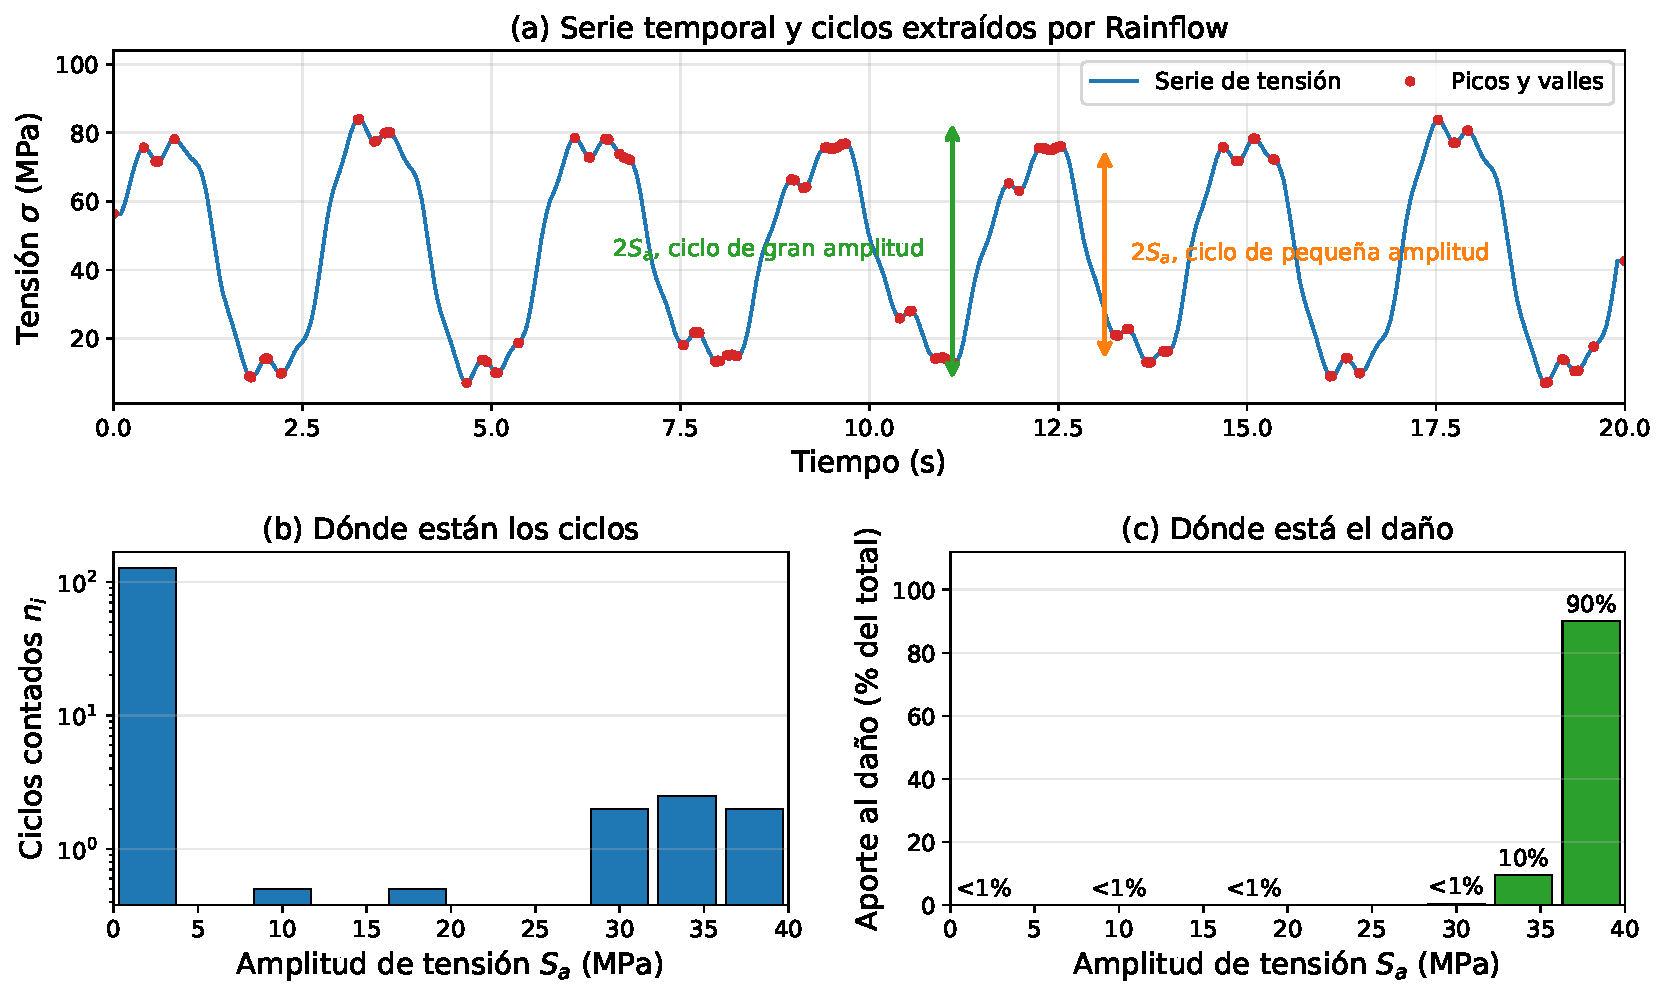
\includegraphics[width=\textwidth]{Figuras/Figuras Antecedentes/rainflow_sn.pdf}
    \caption[Procedimiento de fatiga del Anexo H de la IEC 61400-1.]{Procedimiento de fatiga del Anexo H de la IEC 61400-1 sobre un segmento ilustrativo de serie temporal: (a) ciclos identificados por el conteo Rainflow, (b) espectro de ciclos resultante y (c) aporte de cada rango al daño, evaluado con la curva S-N factoreada (Ec.~\ref{eq:sn_basquin}) para el GFRP empleado en este trabajo.}
    \label{fig:rainflow_sn}
\end{figure}

\newpage
Los paneles (b) y (c) de la Figura~\ref{fig:rainflow_sn} muestran ese efecto sobre el segmento simulado: los dos ciclos de mayor amplitud, asociados a la revolución completa del rotor, concentran el $90\%$ del daño, mientras que los $132$ restantes, de origen turbulento, aportan el resto. De ahí que la verificación de fatiga sea sensible sobre todo a la correcta reproducción de las oscilaciones de gran amplitud.

Resta un aspecto propio de la aplicación a aerogeneradores. Las series simuladas duran minutos y cada una corresponde a una única velocidad de viento, mientras que el daño debe evaluarse sobre veinte años de operación a velocidades que varían continuamente. El objeto que salva esa distancia es el \textit{espectro de carga representativo}: un único recuento de ciclos que resume cuántas veces, y con qué amplitud, se solicita la pala a lo largo de un año típico de operación en el emplazamiento.

Su construcción encadena tres operaciones. La primera es aplicar el conteo Rainflow por separado a la serie de cada velocidad de viento simulada, lo que entrega un espectro parcial, esto es, el número de ciclos $n_i$ por rango de amplitud $S_a$ que la pala experimenta durante los minutos simulados a esa velocidad. La segunda es llevar cada espectro parcial a la escala de un año, multiplicándolo por la razón entre la duración del año y la de la simulación, y por la fracción del año en que el viento permanece en el intervalo de velocidad correspondiente, dato que entrega la distribución de Weibull del emplazamiento (Sección~\ref{sec:recurso_eolico}): así, dos condiciones de viento simuladas durante el mismo tiempo no contribuyen igual al daño anual si una ocurre la mitad del año y la otra apenas unas horas. La tercera operación es sumar los espectros parciales así escalados, rango a rango, con lo que se obtiene el espectro anual. La aplicación numérica de este procedimiento al caso de estudio se desarrolla en la Sección~\ref{sec:anexo_g}.

Con ese espectro, la aplicación de la regla de Miner es inmediata: cada rango de amplitud aporta $n_i/N_i$, donde $N_i$ se lee sobre la curva S-N factoreada, y el daño anual es la suma de esos aportes; multiplicado por la vida de diseño se obtiene el daño acumulado que debe compararse con la unidad.

La vida útil de diseño adoptada para el cálculo es de $20$ años, período que la Sección 6.2 de la IEC 61400-1 establece como vida de diseño mínima para las turbinas de las clases I a III y que constituye, por tanto, el horizonte de referencia frente al cual la norma exige demostrar que $D \leq 1$~\parencite{IEC61400-1}.

Por último, la curva S-N se emplea en su forma factoreada, reduciendo la resistencia mediante el factor parcial de material $\gamma_m = 1{,}7$, valor que la norma asigna a los materiales compuestos con coeficiente de variación de la resistencia entre el $15\%$ y el $20\%$ (Sección 7.6.3.2). El factor parcial aplicado a la carga es, en cambio, $\gamma_f = 1{,}0$ (Sección 7.6.3.1): a diferencia del estado límite último, en fatiga la norma concentra el margen de seguridad en el lado de la resistencia y no en el de la solicitación, por cuanto la incertidumbre dominante proviene de la dispersión de las propiedades del material antes que de la magnitud de las cargas. La curva S-N correspondiente al material empleado en este trabajo, en sus formas nominal y factoreada, se presenta en la Figura~\ref{fig:curva_sn_gfrp}.

\section{Herramientas de simulación aerodinámica}
\label{sec:herramientas}

Una vez definidos el recurso eólico y las condiciones de diseño establecidas por la IEC 61400, resulta necesario emplear herramientas numéricas capaces de reproducir el comportamiento aerodinámico y estructural de la turbina bajo dichas condiciones. Esta sección presenta primero el panorama de los principales métodos disponibles, ordenados de menor a mayor fidelidad, y a continuación el programa QBlade y los submodelos que incorpora, por ser la herramienta sobre la que se apoya el desarrollo posterior. La selección del método y su configuración corresponden a decisiones metodológicas y se justifican en el Capítulo~3.

Esa simulación representa un desafío computacional considerable por la naturaleza inestable de la aerodinámica de las \gls{vawt}: a diferencia de las \gls{hawt}, donde el flujo se aproxima de manera axial y el ángulo de ataque permanece relativamente constante, las palas de un H-rotor experimentan variaciones extremas y cíclicas del ángulo de ataque y atraviesan continuamente su propia estela turbulenta, cinemática que exige resolver fenómenos no lineales como el desprendimiento dinámico de la capa límite y la interacción pala-estela.

\subsection{Métodos aerodinámicos}
\label{sec:metodos_aerodinamicos}

Históricamente, la evaluación aerodinámica de las \gls{vawt} se ha fundamentado en modelos basados en la teoría del momento, siendo el modelo de tubo de corriente múltiple doble (DMST, por sus siglas en inglés)\glsunset{dmst} el más extendido en la ingeniería clásica. Propuesto originalmente por \textcite{Paraschivoiu2002}, el método \gls{dmst} discretiza el rotor en un conjunto de tubos de corriente bidimensionales independientes y divide cada tubo en dos actuadores sucesivos: uno en el semiciclo de barlovento (\textit{upwind}) y otro en el de sotavento (\textit{downwind}). Ambos semiciclos corresponden a las dos mitades del recorrido acimutal identificadas en la Figura~\ref{fig:top_view}: en el de barlovento la pala enfrenta el flujo todavía no perturbado por el rotor, mientras que en el de sotavento lo hace después de que ese mismo flujo ha atravesado la mitad anterior y ha cedido parte de su energía, de modo que llega con velocidad reducida.

Aunque este enfoque permite una estimación algorítmicamente rápida del coeficiente de potencia ($C_p$) y se emplea habitualmente en etapas tempranas de diseño, presenta limitaciones físicas severas: no captura la expansión tridimensional de la estela y pierde precisión de forma drástica en regímenes de alta relación de velocidad de punta ($\lambda$), donde los efectos del flujo inestable dominan el comportamiento del rotor~\parencite{Galinos2015,Tchakoua2015}. Ese umbral no está fijado universalmente, pues la degradación depende también de la solidez del rotor, pero las fuentes lo sitúan hacia el extremo superior del rango en que estas máquinas efectivamente operan: $\lambda = 2$ a $5$ para una configuración H-Darrieus óptima (Tabla~\ref{tab:tabla_vawt}), próximo al \gls{tsr} objetivo de $3{,}8$ de la T1-turbine, de escala comparable a la del caso de estudio (Tabla~\ref{tab:t1_params}). Por su naturaleza cuasi-estática, el DMST sobrestima sistemáticamente el coeficiente de potencia, con valores de $C_p$ que pueden superar $0{,}50$ para configuraciones H-Darrieus, muy por encima del rango validado experimentalmente ($0{,}35\text{--}0{,}45$)~\parencite{Essahraoui2026}. La revisión de \textcite{Islam2008} sobre modelos aerodinámicos para rotores Darrieus de pala recta confirma que el \gls{dmst} no resulta adecuado ni a TSR elevados ni en rotores de alta solidez, mientras que los modelos de vórtices, aun siendo los más precisos, son computacionalmente costosos y pueden presentar problemas de convergencia. Con todo, el bajo costo del \gls{dmst} lo mantiene entre los modelos más extendidos para la estimación preliminar~\parencite{Islam2008}, y es la razón por la que QBlade lo incorpora junto al método de vórtices libres~\parencite{marten2019qblade}.

Para superar estas deficiencias sin incurrir en el costo de las simulaciones viscosas tridimensionales por dinámica de fluidos computacional (CFD, por sus siglas en inglés)\glsunset{cfd}, el estado del arte ha convergido hacia los métodos basados en la teoría de vórtices, entre los cuales el de línea sustentadora con estela de vórtice libre (LLFVW, por sus siglas en inglés)\glsunset{llfvw} se posiciona como una de las herramientas de mayor fidelidad para el análisis aerodinámico de rotores complejos~\parencite{Galinos2015,marten2019qblade}.

Bajo la formulación \gls{llfvw}, las palas del aerogenerador se modelan como líneas de sustentación discretizadas que emiten continuamente filamentos de vorticidad hacia el fluido, según el esquema de la Figura~\ref{fig:llfvw_esquema}. La pala se divide en paneles y se sustituye por una línea situada a un cuarto de cuerda, sobre la que se distribuyen vórtices ligados cuya intensidad reproduce la sustentación local, determinada a partir de la velocidad relativa y de los coeficientes tabulados del perfil~\parencite{marten2019qblade}. De los bordes de cada panel se desprenden dos tipos de filamentos: los vórtices de arrastre (\textit{trailing vortices}), que se extienden aguas abajo y se originan en la variación espacial de la sustentación a lo largo de la envergadura, y los vórtices de desprendimiento (\textit{shed vortices}), que unen transversalmente a los anteriores y se generan en cada paso de tiempo por la variación temporal de la circulación propia del flujo cíclico. El conjunto forma una malla de vorticidad que se convecta, deforma e interactúa libremente en el espacio, sin que su geometría se imponga de antemano, bajo la influencia de sus propias velocidades inducidas. El cálculo de esas velocidades se vuelve singular cuando el punto evaluado cae sobre el propio filamento, por lo que los códigos asignan a cada vórtice un radio de núcleo dentro del cual la velocidad inducida decae suavemente a cero, con lo que se evita la inestabilidad numérica y se representa a la vez el núcleo viscoso real del vórtice~\parencite{marten2019qblade}.

\begin{figure}[H]
    \centering
    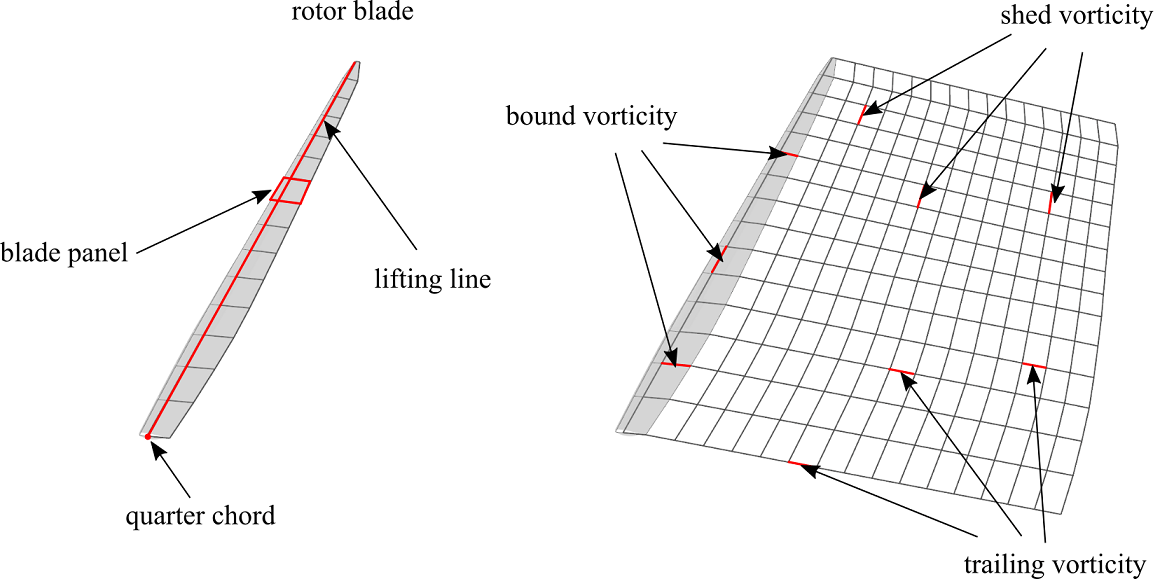
\includegraphics[width=0.7\textwidth]{Figuras/Figuras Antecedentes/qblade_llfvw_bladewake.png}
    \caption[Elementos del modelo de pala y de estela del algoritmo LLFVW.]{Elementos del modelo de pala y de estela del algoritmo LLFVW: panelado de la pala y línea sustentadora a un cuarto de cuerda (izquierda), y vorticidad ligada, de desprendimiento (\textit{shed}) y de arrastre (\textit{trailing}) sobre la malla de estela (derecha). Tomado de la documentación oficial~\parencite{QBladeDocs2024}.}
    \label{fig:llfvw_esquema}
\end{figure}

Resolver la estela de este modo, en lugar de prescribir su geometría, es lo que vuelve al método apropiado para un H-rotor. Como se expuso en la Sección~\ref{sec:aerodinamica}, la pala recorre el semiciclo de sotavento atravesando la estela que ella misma y las restantes palas generaron al pasar por barlovento, fenómeno que \textcite{Ferreira2009} registraron experimentalmente mediante \gls{piv}. La posición de ese encuentro depende de cuánto se ha convectado y deformado la estela en el intervalo transcurrido, de manera que un modelo de estela prescrita no puede reproducirlo. Al calcular esa evolución de forma explícita, el algoritmo \gls{llfvw} entrega la fluctuación de carga asociada al cruce, junto con las pérdidas de punta de pala y el efecto del flujo transversal sobre la estructura~\parencite{Galinos2015,marten2019qblade}: esa fluctuación constituye el ciclo de carga que gobierna la fatiga de la pala y es, por tanto, la magnitud que interesa en este trabajo.

La circulación ligada no se conoce de antemano. La fuerza sobre cada panel depende de la velocidad relativa que este percibe, y esa velocidad incluye la inducción de todos los vórtices del sistema, cuya intensidad es a su vez la incógnita que se busca. El método resuelve esa dependencia mutua de forma iterativa dentro de cada paso temporal: mantiene congelada la geometría de la estela, evalúa una sola vez las velocidades que esta induce sobre los paneles del rotor, y actualiza la circulación ligada hasta que su valor deja de cambiar dentro de una tolerancia prescrita, momento en que las fuerzas del paso quedan determinadas~\parencite{marten2019qblade}. Este lazo se conoce como iteración de circulación, o iteración Gamma por el símbolo $\Gamma$ con que la magnitud se denota, y tanto su tolerancia como el número máximo de iteraciones admitidas constituyen parámetros de configuración del cálculo.

Las familias de métodos descritas no compiten entre sí, sino que ocupan posiciones distintas en lo que \textcite{Essahraoui2026} denominan una jerarquía de fidelidad física, costo computacional y alcance predictivo creciente. La Tabla~\ref{tab:comparacion_metodos} las resume ordenadas de menor a mayor fidelidad, a partir de la revisión de modelos aerodinámicos para rotores Darrieus de pala recta de \textcite{Islam2008} y de la revisión crítica de \textcite{Essahraoui2026}, que actualiza la comparación incorporando los métodos de \gls{cfd}.

\begin{table}[H]
    \centering
    \caption{Comparación de los métodos aerodinámicos para VAWT, ordenados de menor a mayor fidelidad. Elaborada a partir de las revisiones de \textcite{Islam2008} y \textcite{Essahraoui2026}.}
    \label{tab:comparacion_metodos}
    \renewcommand{\arraystretch}{1.2}
    \footnotesize
    \begin{tabular}{p{2.2cm} p{3.3cm} p{3.4cm} p{4.4cm}}
        \hline
        \textbf{Método} & \textbf{Principio} & \textbf{Ventajas} & \textbf{Limitaciones} \\
        \hline
        Momento (DMST) &
        Balance de cantidad de movimiento en tubos de corriente, con factores de inducción independientes para los semiciclos de barlovento y sotavento &
        Costo mínimo; adecuado para barridos paramétricos y estimación preliminar del TSR; captura la asimetría barlovento-sotavento &
        Cuasi-estático: emplea polares estáticas y desatiende la pérdida dinámica y la curvatura de flujo; sobrestima la potencia en rotores de alta solidez y presenta problemas de convergencia a TSR elevados~\parencite{Islam2008,Essahraoui2026} \\
        Vórtices libres (LLFVW) &
        Palas modeladas como líneas sustentadoras que emiten filamentos de vorticidad que convectan libremente en el dominio &
        Resuelve la sustentación inestable, la geometría de la estela y la interacción pala-estela; costo órdenes de magnitud inferior al del CFD resuelto en la pala, compatible con series temporales largas &
        Considerado el más preciso de los modelos clásicos, pero mucho más costoso que los de momento y con posibles problemas de convergencia; supone flujo potencial en la estela e incorpora la viscosidad mediante coeficientes empíricos, por lo que requiere polares externas y modelos semiempíricos de pérdida dinámica~\parencite{Islam2008,Essahraoui2026} \\
        CFD (URANS) &
        Resolución de las ecuaciones de Navier-Stokes promediadas, con cierre de turbulencia $k$-$\omega$ SST o SST transicional &
        Compromiso de referencia en la industria; reproduce el $C_p$ en la zona del máximo con un error de $\pm 5$--$10\%$, que baja a $\pm 3$--$5\%$ con el modelo transicional &
        Costo elevado; sobrestima el torque por debajo del TSR óptimo y los resultados dependen del cierre de turbulencia y de la calidad de la malla~\parencite{Essahraoui2026} \\
        CFD (LES/DES) &
        Resolución directa de las escalas turbulentas mayores, modelando únicamente las menores &
        Máxima fidelidad disponible: error en $C_p$ de $\pm 2$--$3\%$ &
        Costo entre uno y dos órdenes de magnitud superior al del URANS, prohibitivo para el conjunto de casos de carga que exige la norma~\parencite{Essahraoui2026} \\
        \hline
    \end{tabular}
\end{table}

\subsection{El software QBlade}
\label{sec:qblade}

El método \gls{llfvw} descrito se encuentra implementado en QBlade, programa de simulación y diseño de aerogeneradores desarrollado por David Marten en la Technische Universität Berlin, en el marco del trabajo doctoral que documenta su formulación y validación~\parencite{marten2019qblade}. El código está escrito en C++ sobre el entorno multiplataforma Qt y se distribuye de forma gratuita bajo una licencia de código abierto; según el propio autor, al momento de esa publicación era, junto con FAST del NREL, uno de los dos únicos códigos de simulación de aerogeneradores disponibles en esas condiciones, frente a alternativas de uso interno o licencia comercial.

Dos rasgos explican su pertinencia para este trabajo. El primero es que adopta el método de vórtices libres como modelo aerodinámico principal, en lugar de la teoría de momento habitual en los códigos de certificación, precisamente por su mejor comportamiento en condiciones transitorias y extremas de operación. El segundo es que integra el código XFoil~\parencite{drela1989xfoil} y herramientas de extrapolación de polares y de diseño de pala, de modo que la cadena completa, desde la caracterización del perfil hasta la obtención de las cargas aerodinámicas sobre la pala, se resuelve en un mismo entorno.

El programa es, además, de uso extendido: se emplea en cursos de energía eólica de universidades como la propia TU Berlin, DTU y Texas Tech University, y a la fecha de la publicación citada superaba las cien mil descargas, difusión que, según el autor, lo somete a una validación independiente continua por parte de la comunidad de usuarios~\parencite{marten2019qblade}. Las secciones siguientes describen los submodelos de QBlade relevantes para la obtención de cargas sobre la pala.

\subsection{Modelo de pérdida dinámica (Gormont-Berg)}

Como se estableció en la Sección~\ref{sec:dynamicstall}, la pala de una VAWT recorre excursiones de $\alpha$ grandes y rápidas en cada revolución, régimen en el que la pérdida deja de seguir la curva estática y describe en su lugar un lazo de histéresis en $C_l$--$\alpha$. El método \gls{llfvw}, sin embargo, calcula la sustentación de cada panel a partir de la polar estática del perfil, de modo que, sin corrección, subestimaría la carga cuando $\alpha$ aumenta y la sobrestimaría cuando disminuye. El modelo de Gormont-Berg resuelve esto de forma simple y económica en cómputo: en lugar de resolver la capa límite o el vórtice de borde de ataque, aproxima su efecto sobre la sustentación consultando la polar estática en un ángulo desplazado respecto del real, cuya magnitud depende de qué tan rápido varía $\alpha$ en ese instante. La pala retiene así, de forma aproximada, más sustentación de la que indicaría la curva estática mientras $\alpha$ crece, y demora en recuperar el valor estático mientras $\alpha$ decrece, reproduciendo el lazo de histéresis sin resolver la física subyacente.

El modelo original, desarrollado por \textcite{Gormont1973} para rotores de helicóptero, no acota ese desplazamiento, lo que produciría correcciones excesivas ante las excursiones de $\alpha$ propias de una VAWT a TSR bajo, que pueden superar los $30^\circ$ (Sección~\ref{sec:dynamicstall}). La modificación de \textcite{Berg1983} introduce la constante de corrección $A_m$, que atenúa gradualmente el efecto del modelo a medida que $\alpha$ se aleja del ángulo de pérdida estática, adaptándolo a ese rango de excursiones. La formulación completa, con sus expresiones y parámetros, puede consultarse en las fuentes originales y en la documentación de la implementación específica de QBlade~\parencite{Gormont1973,Berg1983,QBladeDocsGormont2024}.

\subsection{Polares aerodinámicas}
\label{sec:polares}

Los métodos basados en líneas sustentadoras, como el \gls{llfvw} descrito en la Sección~\ref{sec:metodos_aerodinamicos}, requieren como información de entrada las características aerodinámicas bidimensionales del perfil alar, representadas mediante curvas polares: conjuntos de datos, organizados como tablas, que registran los coeficientes $C_l$, $C_d$ y $C_m$ definidos en la Sección~\ref{sec:dynamicstall} en función del ángulo de ataque $\alpha$, para un número de Reynolds $Re$ y un número de Mach $M$ determinados. En códigos de simulación como QBlade~\parencite{marten2019qblade}, estos datos se emplean para calcular las fuerzas locales y las variables de rendimiento globales de la turbina. El número de Mach se define y se detalla en la subsección siguiente.

A diferencia de una HAWT, donde el ángulo de ataque se mantiene dentro de un rango acotado, la cinemática del H-rotor descrita en la Sección~\ref{sec:aerodinamica} impone excursiones de $\alpha$ que recorren la totalidad del círculo, desde $-180^\circ$ hasta $+180^\circ$, en particular a TSR bajos y moderados. En consecuencia, la extrapolación de las polares al rango completo de $360^\circ$ de ángulo de ataque no constituye una opción del software sino una necesidad física: el método LLFVW requiere valores definidos de $C_l$, $C_d$ y $C_m$ para todo ángulo de ataque posible, incluyendo los regímenes de pérdida profunda y flujo inverso donde los códigos de capa límite como XFoil o QFoil no convergen. La razón, en términos simples, es que estos códigos suponen que la capa límite del perfil (Sección~\ref{sec:dynamicstall}) permanece delgada y adherida, o a lo sumo levemente separada, condición que les permite acoplar el flujo exterior con la capa límite mediante iteraciones sucesivas hasta encontrar una solución consistente; cuando la separación se vuelve masiva, esa capa deja de ser delgada, el flujo real se vuelve inestable y tridimensional, y ya no existe una solución bidimensional estacionaria que las iteraciones puedan converger a encontrar.

El software QBlade incorpora dos códigos de acoplamiento viscoso-inviscido para calcular las polares de un perfil alar: XFoil~\parencite{drela1989xfoil} y QFoil; estos últimos se describen a continuación.

XFoil resuelve el flujo alrededor del perfil acoplando un método de paneles, que representa el flujo exterior no viscoso, con las ecuaciones integrales de la capa límite, que representan la región viscosa junto a la pared y la estela. Ambas se resuelven de forma simultánea mediante un método de Newton, lo que permite obtener $C_l$, $C_d$ y $C_m$ con un costo muy inferior al de una simulación \gls{cfd}~\parencite{drela1989xfoil}. QFoil es un derivado de XFoil 6.99~\parencite{drelaXfoil699} desarrollado para el análisis de perfiles de aerogeneradores, que conserva esa misma estructura pero modifica el tratamiento de la capa límite y de la estela con el fin de mejorar la robustez numérica y el comportamiento predicho más allá de la pérdida~\parencite{QBladeDocsQFoil2024}.

Las dos modificaciones que explican esa diferencia son el coeficiente de \textit{shear-lag}, que QFoil hace depender del factor de forma de la capa límite en lugar de mantenerlo constante, con lo que la entrada en pérdida se predice de forma más gradual, y la longitud de disipación en la estela, que reduce a la cuarta parte del valor de XFoil para atenuar la sensibilidad del resultado en flujo masivamente separado. Ambos ajustes provienen de la línea de trabajo del código RFoil~\parencite{VanRooij1996} y de las correcciones de arrastre propuestas por \textcite{Ramanujam2016}; el detalle completo de estas y de las restantes diferencias se documenta en~\parencite{QBladeDocsQFoil2024}.

La Tabla~\ref{tab:xfoil_qfoil} resume la comparación entre ambos códigos, y la Figura~\ref{fig:qfoil_vs_xfoil} muestra el efecto práctico sobre un perfil distinto del empleado en este trabajo, el NACA 0020 a $Re = 1 \times 10^6$: las curvas coinciden en la región lineal de flujo adherido y divergen al aproximarse a la pérdida, donde QFoil predice un $C_{l,max}$ menor y un arrastre mayor. Esta comparación es solo entre los dos códigos y no incluye datos experimentales, de modo que por sí sola no permite determinar cuál de las dos predicciones se ajusta mejor a la realidad; esa pregunta solo puede responderse contrastando cada código contra mediciones de túnel de viento para el perfil y el número de Reynolds de interés.

\begin{table}[H]
    \centering
    \caption[Comparación entre XFoil y QFoil.]{Comparación entre XFoil y QFoil. Elaborada a partir de \textcite{QBladeDocsQFoil2024}.}
    \label{tab:xfoil_qfoil}
    \renewcommand{\arraystretch}{1.25}
    \begin{tabular}{p{7.6cm} c c}
        \hline
        \textbf{Característica} & \textbf{XFoil} & \textbf{QFoil} \\
        \hline
        Acoplamiento viscoso-inviscido con método de paneles y capa límite integral & \checkmark & \checkmark \\
        Modelo de transición $e^N$ con $N_{crit}$ ajustable & \checkmark & \checkmark \\
        Coeficiente de \textit{shear-lag} dependiente del factor de forma & --- & \checkmark \\
        Disipación de estela ajustada para flujo separado & --- & \checkmark \\
        Corrección del arrastre en la estela con parámetro de usuario & --- & \checkmark \\
        Reinicialización de la capa límite en cada ángulo del barrido & --- & \checkmark \\
        Convergencia robusta en régimen de pérdida profunda & --- & \checkmark \\
        Resolución máxima del perfil (paneles) & $\sim$300 & 600 \\
        Amplia validación y uso de referencia en la literatura & \checkmark & --- \\
        \hline
    \end{tabular}
\end{table}

\begin{figure}[H]
    \centering
    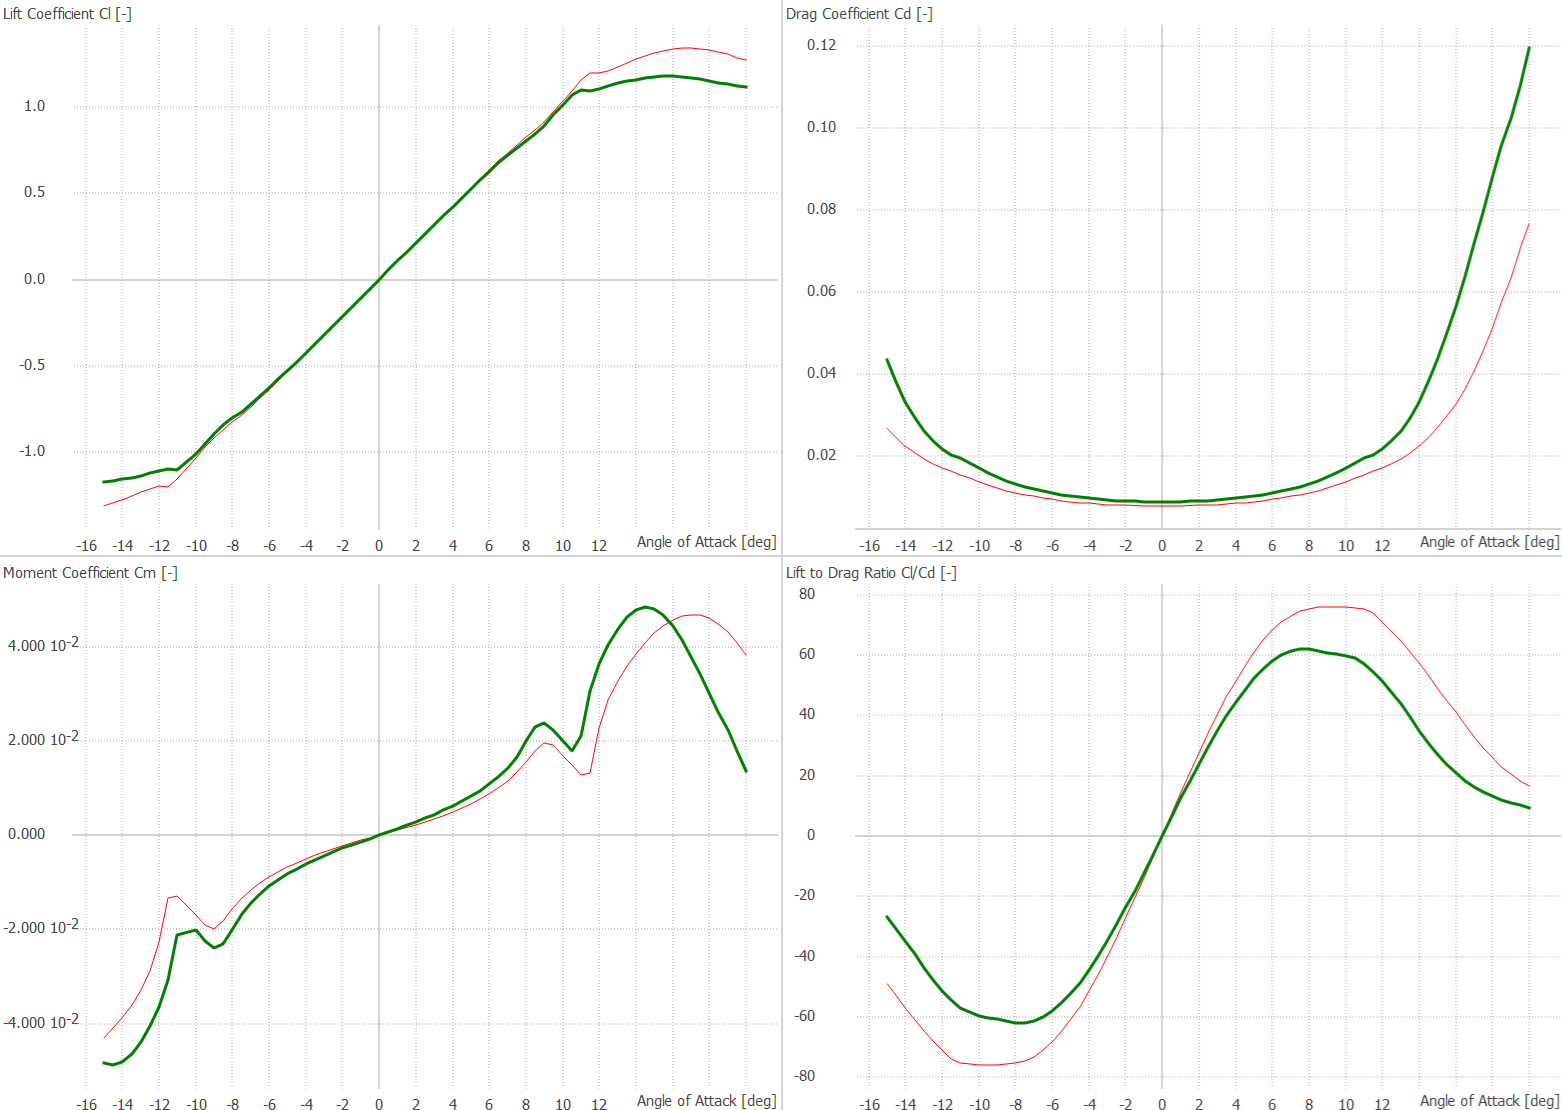
\includegraphics[width=0.92\textwidth]{Figuras/Figuras Antecedentes/qfoil_vs_xfoil.png}
    \caption[Comparación entre QFoil y XFoil para el perfil NACA 0020.]{Comparación entre QFoil (verde) y XFoil (rojo) para el perfil NACA 0020 a $Re = 1 \times 10^6$: coeficientes de sustentación, resistencia y momento, y eficiencia aerodinámica. Tomado de la documentación oficial~\parencite{QBladeDocsQFoil2024}.}
    \label{fig:qfoil_vs_xfoil}
\end{figure}

Esta distinción es relevante en las \gls{vawt}, donde las palas recorren excursiones de ángulo de ataque muy amplias en un solo ciclo de rotación y operan de forma habitual en pérdida profunda. En ese régimen es donde XFoil presenta mayores dificultades de convergencia y donde las diferencias de la Figura~\ref{fig:qfoil_vs_xfoil} se vuelven determinantes, razón por la cual QFoil resulta preferible para el cálculo de polares destinadas a una \gls{vawt}. La propia documentación advierte, no obstante, que QFoil no es numéricamente equivalente a XFoil y que sus resultados deben revalidarse contra datos experimentales antes de emplearse~\parencite{QBladeDocsQFoil2024}. Esa es la comparación pertinente aquí: no XFoil contra QFoil, sino QFoil contra mediciones reales del perfil NACA 0018 en el rango de Reynolds de interés. Los datos experimentales de referencia se presentan en la Sección~\ref{sec:caracterizacion_aero}, y su contraste cuantitativo con las polares de QFoil, que respalda la configuración finalmente adoptada, se muestra en el Capítulo~4 (Figura~\ref{fig:comparacion_ncrit_250k}).

\subsubsection{Parámetros de simulación aerodinámica}

\textbf{Número de Mach ($M$):} Representa la relación entre la velocidad del flujo y la velocidad del sonido, y cuantifica cuánto varía la densidad del aire al acelerarse sobre el perfil. Un flujo se considera incompresible cuando $M < 0{,}3$, umbral bajo el cual la variación de densidad respecto de la condición de reposo se mantiene por debajo del $5\%$ y puede despreciarse~\parencite{Anderson2016}. Los códigos basados en el método de paneles, como XFoil y QFoil, incorporan la corrección de compresibilidad de Kármán-Tsien~\parencite{Karman1941,Tsien1939} para extender su validez a números de Mach mayores; dicha corrección deja de ser fiable cuando el número de Mach local sobre el perfil supera aproximadamente $1{,}05$, condición en que aparecen regiones supersónicas y ondas de choque que el método no resuelve~\parencite{drelaXfoil699}.

En una \gls{vawt} el número de Mach relevante no es el del viento incidente sino el asociado a la velocidad relativa $W$, que combina la velocidad del viento con la velocidad tangencial de la pala y resulta considerablemente mayor. Aun así, al ser la velocidad de punta de una máquina de eje vertical sustancialmente menor que la de una \gls{hawt} de tamaño comparable, estos rotores operan siempre en régimen claramente subsónico y los efectos de compresibilidad resultan despreciables.

\textbf{Parámetro de Transición ($N_{crit}$):} Es el factor principal del modelo de transición $e^N$ utilizado para predecir el cambio natural de la capa límite de régimen laminar a turbulento sobre el perfil alar. El modelo se apoya en que, antes de la transición, las pequeñas perturbaciones presentes en la capa límite laminar (las ondas de Tollmien-Schlichting) se amplifican de forma exponencial al avanzar sobre el perfil. Si $A_0$ es la amplitud de la perturbación más inestable en el punto donde comienza a crecer y $A$ su amplitud en una posición posterior, el factor de amplificación $n$ se define según la Ec.~\ref{eq:en_transicion}:

\begin{equation}
n = \ln\left( \frac{A}{A_0} \right)
\label{eq:en_transicion}
\end{equation}

El criterio supone que la transición ocurre donde $n$ alcanza el valor umbral $N_{crit}$, de modo que este parámetro es el logaritmo del factor de amplificación admisible antes de que el flujo se vuelva turbulento: $N_{crit} = 9$, por ejemplo, corresponde a una amplificación de $e^{9} \approx 8100$ veces~\parencite{drela1989xfoil}. Su valor no es una propiedad del perfil sino del entorno: cuanto mayor sea la turbulencia o la rugosidad del flujo incidente, mayores serán las perturbaciones iniciales y menor la amplificación necesaria para desencadenar la transición, por lo que $N_{crit}$ disminuye. Valores elevados se asocian a flujos libres de perturbaciones, como en planeadores, y valores bajos a entornos de mayor turbulencia; la Tabla~\ref{tab:ncrit_values} recoge los valores de referencia recomendados según las condiciones del flujo.

Su valor tiene un efecto directo sobre las curvas polares del perfil: un $N_{crit}$ elevado retrasa la transición de la capa límite y se traduce en un mayor coeficiente de sustentación máximo ($C_{l,max}$), un ángulo de pérdida más tardío y un coeficiente de arrastre reducido en el rango lineal previo a la pérdida, mientras que valores bajos anticipan la transición turbulenta, reducen el $C_{l,max}$, desplazan la pérdida hacia ángulos de ataque menores e incrementan el arrastre por fricción superficial~\parencite{drela1989xfoil}.

\begin{table}[H]
    \centering
    \caption{Valores de $N_{crit}$ de referencia según la documentación de Xfoil.}
    \label{tab:ncrit_values}
    \begin{tabular}{lc}
        \hline
        \textbf{Condición del Flujo} & \textbf{Valor $N_{crit}$}\\
        \hline
        Soplado en planeador (sailplane)   & 12 -- 14 \\
        Motoplaneador (motorglider)        & 11 -- 13 \\
        Túnel de viento limpio             & 10 -- 12 \\
        Túnel de viento promedio           & 9        \\
        Túnel de viento con turbulencia    & 4 -- 8   \\
        \hline
    \end{tabular}
\end{table}

La física del perfil es sensible al número de Reynolds, especialmente en regímenes bajos y moderados. A $Re$ entre $1 \times 10^6$ y $3 \times 10^6$, es frecuente la formación de una burbuja de separación laminar: la capa límite, todavía laminar, se separa de la superficie antes de haber transicionado a turbulenta, pero la capa de corte ya separada sí transiciona, y esa capa turbulenta, con mayor cantidad de movimiento, logra readherirse aguas abajo. El resultado es una pequeña región cerrada de recirculación entre el punto de separación laminar y el de readherencia turbulenta, distinta de la separación progresiva que avanza desde el borde de fuga descrita en la Sección~\ref{sec:dynamicstall} (Figura~\ref{fig:stall_progresion}). Aunque de extensión pequeña, esta burbuja modifica la presión efectiva sobre el extradós y con ello el coeficiente de sustentación máximo ($C_{l,max}$) y el comportamiento de la pérdida~\parencite{drela1989xfoil}. A números de Reynolds más altos, en cambio, la transición ocurre de forma casi inmediata y la burbuja prácticamente desaparece.

\textbf{Transición Forzada (Forced Transition):} Parámetros que definen la posición exacta (expresada como una fracción de la cuerda, $x/c$) en la cual se fuerza la transición a flujo turbulento en la superficie superior (\textit{Forced Top Transition}) e inferior (\textit{Forced Bottom Transition}) del perfil, anulando el cálculo del modelo de transición natural en dicha zona. Se emplean conceptualmente para simular la presencia de cintas de transición (\textit{trips}) físicas o pérdidas de rendimiento por suciedad y rugosidad acumulada~\parencite{drela1989xfoil}.

La Tabla~\ref{tab:resumen_params_polares} resume los parámetros que gobiernan el cálculo de polares y su efecto sobre los resultados aerodinámicos.

\begin{table}[H]
    \centering
    \caption{Resumen de parámetros que gobiernan el cálculo de polares aerodinámicas.}
    \label{tab:resumen_params_polares}
    \begin{tabular}{lcc}
        \hline
        \textbf{Parámetro} & \textbf{Fenómeno físico} & \textbf{Símbolo} \\
        \hline
        Número de Reynolds & Viscosidad & $Re$ \\
        Número de Mach & Compresibilidad & $M$ \\
        $N_{crit}$ & Transición laminar-turbulenta & $N_{crit}$ \\
        Transición forzada & Fijación artificial de la transición & $x/c$ \\
        \hline
    \end{tabular}
\end{table}

\subsection{Caracterización aerodinámica y datos de validación}
\label{sec:caracterizacion_aero}

Dado que los códigos de cálculo descansan en modelos semiempíricos de la capa límite, sus polares requieren contraste con mediciones. El ensayo de referencia para ello es el túnel de viento, donde el perfil se monta en condiciones bidimensionales y se registran las fuerzas mientras varía el ángulo de ataque.

El estudio de \textcite{Bianchini2015} constituye un antecedente pertinente para la caracterización aerodinámica de perfiles en \gls{vawt}, al obtener las polares definidas en la Sección~\ref{sec:dynamicstall} en el rango completo de $360^\circ$ de ángulo de ataque para el perfil NACA 0018. Los ensayos se realizaron en un túnel de viento de baja turbulencia, con intensidad inferior al $0{,}1\%$, para números de Reynolds entre $6{,}0 \times 10^4$ y $3{,}0 \times 10^5$. Los coeficientes de sustentación y resistencia medidos se contrastan punto a punto con los obtenidos mediante simulaciones de \gls{cfd} (Figura~\ref{fig:comparacion_resultados_paper}), con concordancia general en todo el rango y discrepancias acotadas, explícitamente reportadas por los autores, entre $150^\circ$ y $180^\circ$ para la sustentación y a ángulos positivos elevados para la resistencia, nivel de correspondencia que permite emplear sus polares como referencia para la validación de modelos numéricos. El estudio identificó, asimismo, deficiencias en la base de datos histórica de Sheldahl y Klimas (1981) para este perfil, y concluye que el modelo de Montgomerie ofrece el mejor desempeño entre los métodos de extrapolación evaluados.

\begin{figure}[h]
\centering
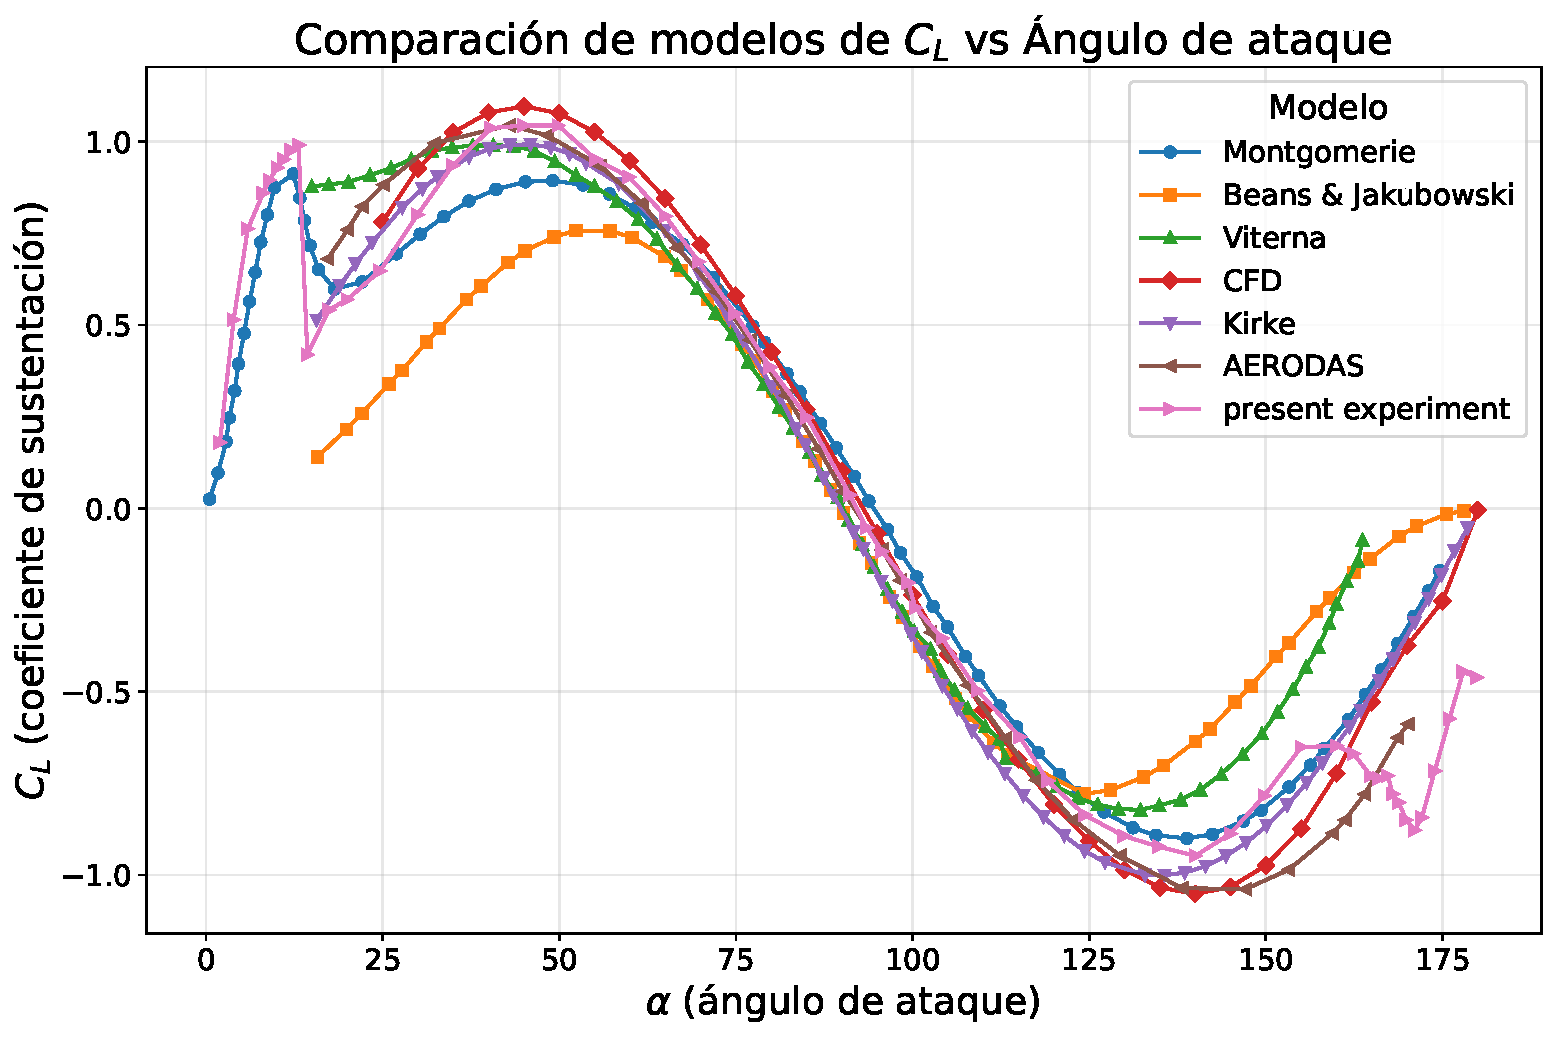
\includegraphics[width=0.8\textwidth]{Figuras/Figuras Antecedentes/LC AoA comparacion.pdf}
\caption{Comparación de polares del perfil NACA 0018 entre modelos de predicción.}
\label{fig:comparacion_resultados_paper}
\end{figure}

\subsection{Extrapolación de polares aerodinámicas}

Debido a que los códigos de cálculo, por la razón expuesta en la Sección~\ref{sec:polares}, dejan de converger una vez que la separación se vuelve masiva, generan polares confiables solo hasta la pérdida y un rango limitado más allá de ella. Como la caracterización del rendimiento aerodinámico de la turbina requiere $C_l$, $C_d$ y $C_m$ definidos en los $360^\circ$ de operación, resulta necesario extender esos datos mediante un modelo de extrapolación.

La literatura ofrece más de uno; se repasan aquí los dos más difundidos, que responden a principios de construcción distintos. El de \textcite{viterna1982theoretical} no describe la física del flujo separado, sino que deduce la forma de la curva imponiendo tres condiciones sobre el tramo posterior a la pérdida: continuidad con la polar adherida en el ángulo de pérdida, un coeficiente de torque constante a lo largo de todo ese tramo, y el valor de arrastre que corresponde a $90^\circ$ según la relación de aspecto de la pala. La segunda condición es la que fija la forma, y proviene de una observación experimental sobre rotores regulados por pérdida, esto es, aquellos que a partir de cierta velocidad de viento operan intencionalmente en pérdida para limitar la potencia captada: en ellos el torque medido más allá de la pérdida resulta prácticamente independiente de la velocidad del viento y, por tanto, del ángulo de ataque. Las expresiones que satisfacen las tres condiciones son las Ecs.~\ref{eq:viterna_cl} y~\ref{eq:viterna_cd}:

\begin{equation}
C_l = A_1 \sin(2\alpha) + A_2 \frac{\cos^2\alpha}{\sin\alpha}
\label{eq:viterna_cl}
\end{equation}
\begin{equation}
C_d = B_1 \sin^2\alpha + B_2 \cos\alpha
\label{eq:viterna_cd}
\end{equation}

donde $A_1$, $A_2$, $B_1$ y $B_2$ quedan completamente determinados por solo cuatro datos del perfil: el ángulo de pérdida $\alpha_s$, los coeficientes $C_{l,s}$ y $C_{d,s}$ en ese ángulo, y la relación de aspecto de la pala $AR = R/c$, que fija el arrastre a $90^\circ$ mediante la correlación empírica $C_{d,90} = 1{,}11 + 0{,}018\,AR$. Fijado el punto de pérdida, la curva completa queda determinada, sin parámetros adicionales para ajustar su forma. Esa rigidez es coherente con el propósito para el que fue concebido, capturar el torque en pérdida frontal de una HAWT, pero no con lo que exige una VAWT: valores físicamente consistentes de $C_l$, $C_d$ y $C_m$ en los $360^\circ$ completos, incluido el flujo inverso, régimen donde la hipótesis que origina el modelo, un torque post-pérdida constante, deja de tener sentido.

El modelo de Montgomerie parte de un principio distinto. En lugar de deducir la curva de una condición sobre el torque, la construye como una mezcla de las dos soluciones límite que sí se conocen: la recta de flujo potencial, válida mientras el flujo permanece adherido, y la curva de placa plana delgada, válida cuando la separación es completa, ponderadas por una función de transición que las une de forma continua en todo el círculo~\parencite{montgomerie2004methods}. Al no imponer condición alguna sobre el torque, la construcción no privilegia ningún tramo de la polar y admite parámetros de ajuste independientes, detallados en la subsección siguiente: además del punto de transición, la amplitud del arrastre en placa plana ($C_{d90}$) y la suavidad con que la curva se aproxima a ese régimen a cada lado ($A^+$, $A^-$, $B^+$, $B^-$). Esa libertad es la que permite reproducir el comportamiento asimétrico de un perfil en pérdida profunda y flujo inverso, y la que \textcite{Bianchini2015} identifican como la razón por la que Montgomerie reproduce mejor sus datos experimentales en el rango completo de $360^\circ$. La Tabla~\ref{tab:extrapolacion_metodos} contrasta ambos principios de construcción.

\begin{table}[H]
    \centering
    \caption[Comparación de los métodos de extrapolación de polares.]{Comparación de los principios de construcción de los métodos de extrapolación de polares. Elaborada a partir de \textcite{viterna1982theoretical}, \textcite{montgomerie2004methods} y \textcite{Bianchini2015}.}
    \label{tab:extrapolacion_metodos}
    \renewcommand{\arraystretch}{1.2}
    \footnotesize
    \begin{tabular}{p{1.9cm} p{4.0cm} p{3.2cm} p{4.2cm}}
        \hline
        \textbf{Método} & \textbf{Principio de construcción} & \textbf{Grados de libertad} & \textbf{Alcance y limitaciones} \\
        \hline
        Viterna &
        Deduce el tramo posterior a la pérdida imponiendo continuidad con la polar adherida, torque constante más allá del ángulo de pérdida y el arrastre que corresponde a $90^\circ$~\parencite{viterna1982theoretical} &
        Ninguno: el punto de pérdida y la relación de aspecto determinan los cuatro coeficientes y, con ellos, toda la curva &
        Concebido para el tramo en pérdida de una HAWT regulada por pérdida; sus expresiones no incorporan parámetros que distingan un lado de la polar del otro, y la hipótesis de torque constante pierde sentido en flujo inverso \\
        Montgomerie &
        Interpola entre la recta de flujo potencial y la curva de placa plana delgada mediante una función de transición continua en todo el círculo~\parencite{montgomerie2004methods} &
        Punto de transición, $C_{d90}$ y los parámetros de acoplamiento $A^{\pm}$ y $B^{\pm}$, ajustables por separado a cada lado de la polar &
        Formulado para el rango completo de $\pm 180^\circ$; exige calibrar esos parámetros contra datos del perfil, y en el contraste experimental sobre el NACA 0018 resultó el de mejor desempeño entre los métodos evaluados~\parencite{Bianchini2015} \\
        \hline
    \end{tabular}
\end{table}

\subsubsection{Modelo Montgomerie y sus parámetros de configuración}

El modelo, desarrollado en la Agencia Sueca de Investigación de Defensa (FOI), formula esa interpolación mediante las expresiones siguientes.

Función de transición ($f$): define el peso relativo entre el régimen de flujo adherido y el separado, según la Ec.~\ref{eq:mont_f}:
\begin{equation}
f = \frac{1}{1 + k \cdot \Delta\alpha^4}
\label{eq:mont_f}
\end{equation}

donde $\alpha$ corresponde al ángulo de ataque; $\Delta\alpha$ es su desplazamiento respecto al punto en que la curva original se aparta de la recta de flujo potencial, esto es, respecto al inicio de la separación, y $k$ es una constante de ajuste que se calibra con dos puntos de la curva dada. Mientras $\alpha$ se mantiene dentro del tramo adherido, $\Delta\alpha \approx 0$ y $f \approx 1$; más allá de ese punto, $\Delta\alpha$ crece y $f$ decae rápidamente hacia $0$, por la potencia cuarta del denominador.

Coeficiente de sustentación ($C_l$): Se obtiene interpolando entre la línea de flujo potencial ($t$) y la curva de placa plana ($s$), según la Ec.~\ref{eq:mont_cl}:
\begin{equation}
C_L = f \cdot t + (1 - f) \cdot s
\label{eq:mont_cl}
\end{equation}

La Figura~\ref{fig:montgomerie_st} ilustra esta interpolación para un perfil simétrico. El panel (a) muestra la forma de $f$, una meseta en $1$ dentro del tramo adherido que cae abruptamente una vez superado el punto de transición $\alpha_M$; el panel (b), las dos curvas que $f$ pondera, la recta $t(\alpha)$ y la curva de placa plana $s(\alpha)$, junto con el resultado de la Ec.~\ref{eq:mont_cl}: mientras $f \approx 1$, $C_l$ coincide con la recta $t$; una vez que $f$ cae, converge hacia la curva acotada $s$, evitando que la recta, que de otro modo crecería sin límite, se extienda a ángulos donde ya no representa flujo adherido.

\begin{figure}[H]
    \centering
    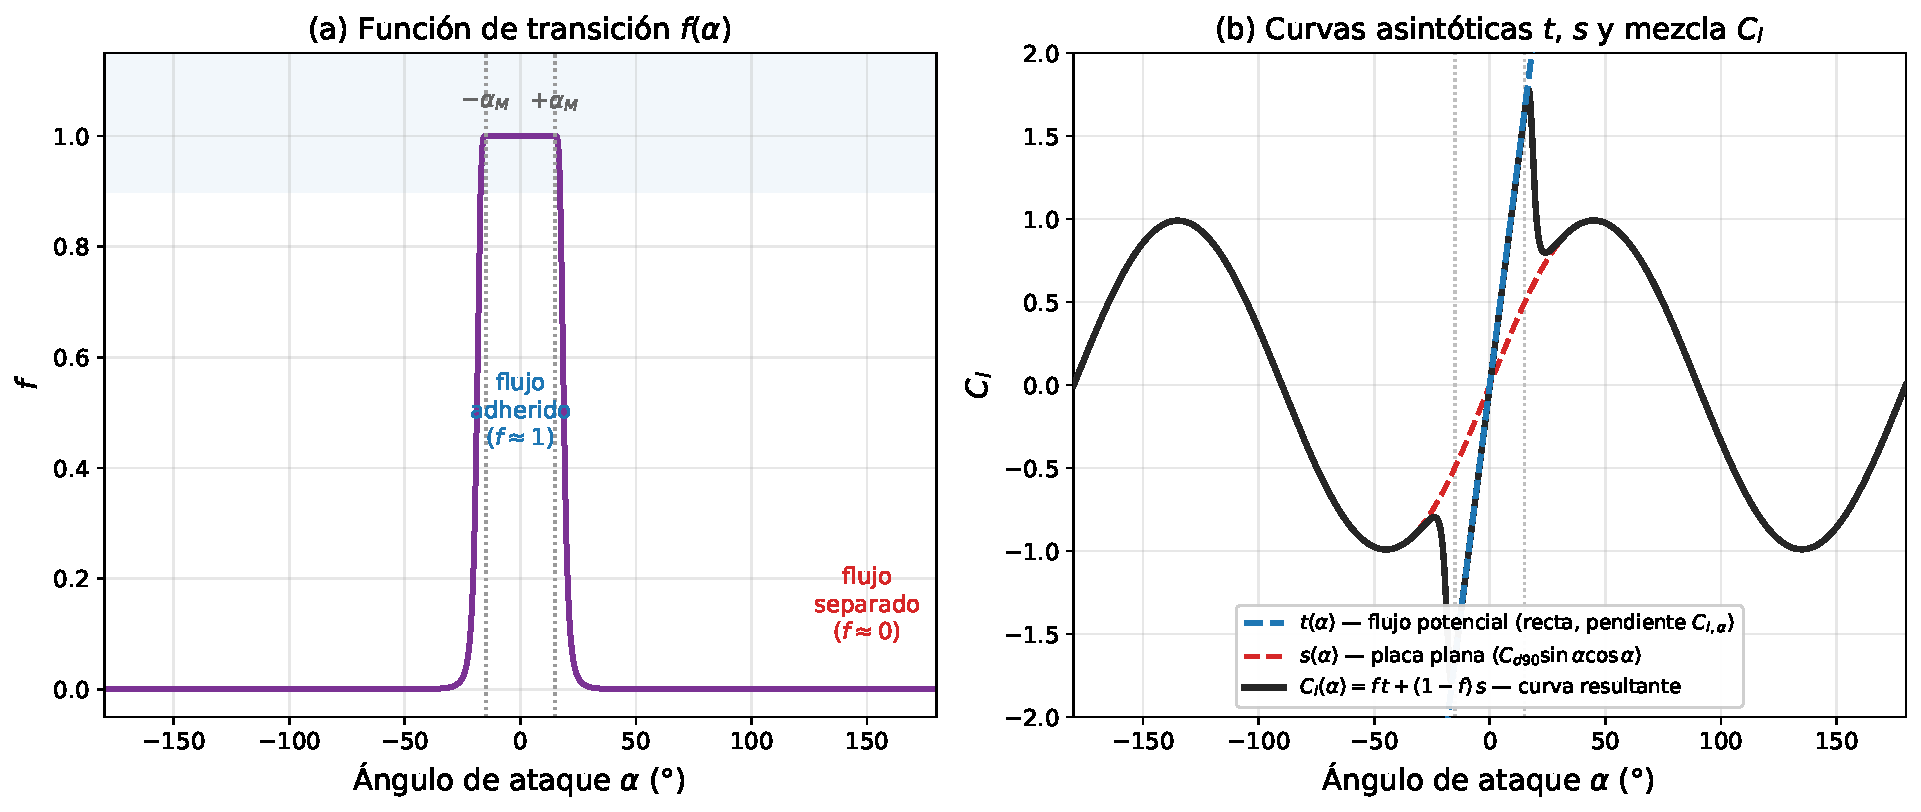
\includegraphics[width=0.95\textwidth]{Figuras/Figuras Antecedentes/montgomerie_st.pdf}
    \caption[Función de transición e interpolación entre flujo potencial y placa plana en el modelo de Montgomerie.]{Ilustración del modelo de Montgomerie para un perfil simétrico: (a) función de transición $f(\alpha)$ y (b) curvas de flujo potencial $t(\alpha)$, placa plana $s(\alpha)$ y sustentación resultante $C_l(\alpha)$.}
    \label{fig:montgomerie_st}
\end{figure}

Coeficiente de arrastre ($C_d$): queda fijado por el parámetro $C_{d90}$, el coeficiente de resistencia del perfil a $\alpha = 90^\circ$, esto es, cuando se comporta como una placa plana orientada perpendicularmente al flujo, valor que define la amplitud de toda la curva de arrastre en régimen separado según la Ec.~\ref{eq:mont_cd}:
\begin{equation}
C_{D, thinPlate} = C_{d90} \cdot \sin^2(\alpha)
\label{eq:mont_cd}
\end{equation}

Coeficiente de momento ($C_m$): se calcula utilizando un brazo de momento variable que asegura el realismo físico del punto de aplicación de la fuerza en pérdida profunda.

A diferencia del arrastre a $90^\circ$, que fija solo la amplitud de la curva de placa plana, los parámetros de acoplamiento $A^+$, $A^-$, $B^+$ y $B^-$ controlan la forma y la suavidad con que la curva transiciona hacia ese régimen en cada lado de la polar, para ángulos positivos y negativos respectivamente. Este conjunto, ausente en modelos más rígidos como el de Viterna, es el que permite reproducir curvas asimétricas o con transiciones de distinta suavidad a cada lado del punto de pérdida.

Estos parámetros, junto con la pendiente de sustentación determinada a partir de las curvas polares, definen la configuración del modelo de Montgomerie.

\section{Análisis estructural y criterios de falla}
\label{sec:analisis-estructural}

Una pala de aerogenerador es, estructuralmente, una viga sometida a solicitaciones de naturaleza distinta. Las cargas aerodinámicas, generadas por la interacción del perfil con el flujo incidente, varían continuamente en el tiempo; las inerciales, esto es, la gravitatoria y la centrífuga, se mantienen estacionarias mientras la velocidad de rotación no cambia~\parencite{Galinos2015}. En un H-rotor, cuyas palas rectas son paralelas al eje de rotación, la fuerza centrífuga actúa en dirección perpendicular a la envergadura, según se describió en la Sección~\ref{sec:vtip}. Las uniones a los struts constituyen los apoyos de la pala, de modo que esta flecta en el vano comprendido entre ellas y en los tramos que quedan en voladizo hacia las puntas. Verificar la pala consiste, en esencia, en traducir esas solicitaciones en un estado de tensiones y deformaciones dentro del material, y contrastarlo con lo que el material admite: su resistencia frente a la carga máxima, su estabilidad frente al pandeo y su capacidad de soportar la repetición de ciclos a lo largo de la vida útil.

\subsection{Configuración estructural de una pala}

Antes de discutir materiales conviene fijar la nomenclatura de los elementos que componen una pala, ya que de ellos depende cómo se reparten las tensiones. La sección transversal se organiza en dos partes con funciones distintas, según se ilustra en la Figura~\ref{fig:estructura_pala}: el contorno aerodinámico, formado por pieles relativamente delgadas que definen la forma del perfil pero no están dimensionadas para tomar por sí solas la flexión, y un elemento longitudinal interno en que estas se apoyan, un larguero o un conjunto de almas, que recorre la envergadura y absorbe una parte sustancial de la carga~\parencite{Brondsted2005}.

\begin{figure}[H]
    \centering
    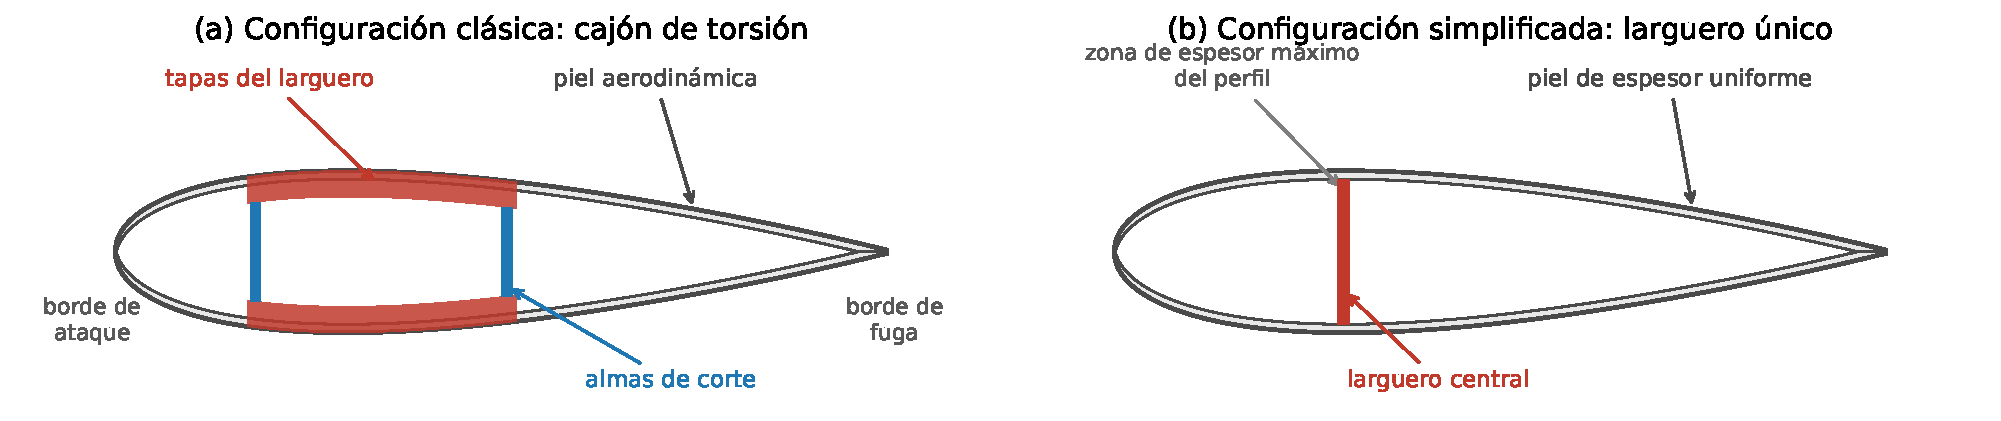
\includegraphics[width=\textwidth]{Figuras/Figuras Antecedentes/estructura_pala.pdf}
    \caption[Elementos estructurales de una pala de aerogenerador en sección transversal.]{Elementos estructurales de una pala de aerogenerador en sección transversal, en dos configuraciones habituales. Nomenclatura según la sección de referencia descrita por \textcite{Brondsted2005}.}
    \label{fig:estructura_pala}
\end{figure}

El reparto de funciones sigue una lógica sencilla. Al flexionarse la pala, las tensiones normales de tracción y compresión se concentran en las caras superior e inferior, las más alejadas del eje neutro, esto es, de la línea de la sección que no se alarga ni se acorta al flectar y que, por tanto, no está sometida a tensión; por eso la configuración clásica de las palas de gran tamaño (Figura~\ref{fig:estructura_pala}a) engrosa el laminado precisamente allí, formando las \textit{tapas del larguero}, y las une mediante una o dos \textit{almas de corte}, elementos verticales que transmiten el esfuerzo cortante y evitan que las tapas se desplacen una respecto de la otra. El conjunto constituye un cajón de torsión que aporta la rigidez a flexión y a torsión de la pala. En palas rectas de menor tamaño resulta habitual una configuración más simple (Figura~\ref{fig:estructura_pala}b), con piel de espesor prácticamente uniforme y un único larguero situado en la zona de espesor máximo del perfil, donde el brazo respecto del eje neutro es mayor. Los extremos de la sección reciben nombres propios: el \textit{borde de ataque}, redondeado, y el \textit{borde de fuga}, afilado, que por su geometría delgada aporta poco a la rigidez y suele ser una zona crítica de fabricación.

Esta arquitectura explica por qué la piel, además de resistencia, requiere estabilidad: los paneles entre elementos de apoyo trabajan en compresión en la cara comprimida de la pala y pueden fallar por pandeo local, es decir, por abolladura, antes de alcanzar la resistencia del material, de modo que el dimensionamiento no depende solo de cuánta tensión soporta el laminado, sino también de la distancia entre elementos rigidizadores.

\subsection{Materiales empleados en palas de aerogeneradores}
\label{sec:materiales_palas}

La selección de material para una pala responde a tres requisitos simultáneos: rigidez elevada, para mantener las deflexiones acotadas y preservar la forma aerodinámica; densidad baja, ya que la propia masa de la pala genera cargas inerciales y gravitatorias; y buen comportamiento a fatiga, dado que la pala acumula del orden de $10^8$ a $10^9$ ciclos durante su vida útil~\parencite{Brondsted2005}. Estos requisitos compiten entre sí, y su compromiso se resume en un índice de mérito que para una viga en flexión vale $M_b = E^{1/2}/\rho$, donde $E$ es el módulo elástico y $\rho$ la densidad: cuanto mayor sea $M_b$, mayor rigidez se obtiene por unidad de masa. Aplicado sobre el conjunto de los materiales de ingeniería, este criterio descarta a la mayoría y, junto con la condición adicional de un módulo absoluto del orden de $10$ a $20$~GPa para limitar las deflexiones, deja como candidatos a los materiales compuestos~\parencite{Brondsted2005}.

La Tabla~\ref{tab:materiales_palas} recoge las propiedades de las fibras candidatas y de los laminados que resultan de combinarlas con una matriz polimérica, esto es, la resina que envuelve las fibras y las solidariza entre sí para que trabajen en conjunto. La fibra de vidrio tipo E ofrece una combinación equilibrada de rigidez moderada, resistencia alta y densidad moderada, a un costo sustancialmente menor, lo que lo ha mantenido como la fibra más utilizada. El carbono casi cuadruplica el módulo del laminado y reduce su densidad, con lo que su índice de mérito resulta unas tres veces superior; su adopción creciente responde tanto al aumento de tamaño de las palas, donde el peso propio se vuelve limitante, como a la caída de su precio~\parencite{Brondsted2005}. Las fibras de aramida, polietileno y celulosa presentan índices de mérito intermedios y densidades bajas, pero ninguna ha alcanzado un desarrollo industrial que las haga viables en palas de gran tamaño.

\begin{table}[H]
    \centering
    \caption[Propiedades de fibras y laminados candidatos para palas de aerogeneradores.]{Propiedades de fibras y laminados candidatos para palas de aerogeneradores. Los laminados corresponden a fibras alineadas en matriz polimérica, con una proporción de fibra del $50\%$ en volumen. Adaptada de \textcite{Brondsted2005}.}
    \label{tab:materiales_palas}
    \renewcommand{\arraystretch}{1.2}
    \footnotesize
    \begin{tabular}{l c c c c c c c}
        \hline
        & \multicolumn{3}{c}{\textbf{Fibra}} & \multicolumn{4}{c}{\textbf{Laminado}} \\
        \cmidrule(lr){2-4} \cmidrule(lr){5-8}
        \textbf{Fibra} & $E_f$ & $\sigma_f$ & $\rho_f$ & $E_c$ & $\sigma_c$ & $\rho_c$ & $E_c^{1/2}/\rho_c$ \\
        & (GPa) & (MPa) & (g/cm$^3$) & (GPa) & (MPa) & (g/cm$^3$) & \\
        \hline
        Vidrio tipo E & 72  & 3500 & 2{,}54 & 38  & 1800 & 1{,}87 & 3{,}3 \\
        Carbono      & 350 & 4000 & 1{,}77 & 176 & 2050 & 1{,}49 & 8{,}9 \\
        Aramida      & 120 & 3600 & 1{,}45 & 61  & 1850 & 1{,}33 & 5{,}9 \\
        Polietileno  & 117 & 2600 & 0{,}97 & 60  & 1350 & 1{,}09 & 7{,}1 \\
        Celulosa     & 80  & 1000 & 1{,}50 & 41  & 550  & 1{,}35 & 4{,}7 \\
        \hline
    \end{tabular}
\end{table}

La pala del caso de estudio ya está definida por el fabricante: se trata de un polímero reforzado con fibra de vidrio (GFRP) con tejido bidireccional a $\pm 45^\circ$, fabricado por infusión al vacío, técnica que permite obtener fracciones volumétricas de fibra elevadas con baja porosidad.

\subsection{Comportamiento mecánico del laminado y criterios de falla}
\label{sec:comportamiento_laminado}

Dos rasgos del comportamiento de un compuesto de fibra de vidrio condicionan la forma en que se verifica la pala. El primero es que se trata de un material \textit{frágil}, es decir, a diferencia de un material dúctil, que fluye plásticamente y redistribuye tensiones antes de romper, el laminado responde de forma prácticamente lineal hasta la rotura cuando la carga la toman las fibras, sin una meseta de fluencia que advierta la proximidad del fallo, y la rotura sobreviene por fractura frágil de las fibras y de la matriz que las envuelve~\parencite{Huh2012,Moraras2023}. La Figura~\ref{fig:curva_esfuerzo_deformacion} recoge esa respuesta para el material de la pala del caso de estudio. Esa linealidad simplifica el análisis, pues permite tratar la respuesta como proporcional a la carga, pero elimina el margen de aviso que ofrece la plastificación y obliga a apoyarse en los factores parciales de seguridad para cubrir la incertidumbre.

El segundo rasgo es la \textit{ortotropía}: las propiedades del laminado dependen de la dirección, con valores máximos en la dirección de las fibras y sustancialmente menores en la transversal y en corte, donde la carga la toma principalmente la matriz. La rigidez decae de forma continua a medida que el ángulo entre la fibra y la carga crece de $0^\circ$ a $90^\circ$~\parencite{Brondsted2005,Huh2012}. Los ensayos sobre laminados de pala miden ese efecto: en placas de fibra de vidrio con tejido a $0^\circ/90^\circ$, la resistencia obtenida al cargar a $45^\circ$ respecto de las fibras cae por debajo de un tercio de la medida en la dirección de estas~\parencite{Moraras2023}, y la mayor resistencia a tracción corresponde a la dirección longitudinal, la de alineación de las fibras~\parencite{Ahmed2021}. Un mismo estado de carga puede ser entonces inofensivo o crítico según cómo esté orientado respecto de las fibras, de modo que no basta con conocer su magnitud y se requiere además la distribución espacial del estado tensional. Esa es la razón de fondo por la que la verificación no puede resolverse con un modelo unidimensional de viga, a lo que se suma que, en las conexiones con los struts, la hipótesis de secciones planas deja de ser válida, ya que las cargas concentradas generan distribuciones de tensión que un modelo de viga no resuelve.

Conviene anticipar aquí hasta dónde llega la verificación que este trabajo realiza con esa base. Aprovechar plenamente la ortotropía exige un criterio de fallo direccional aplicado capa a capa, del tipo de los de Puck o Tsai-Wu, y para eso hace falta conocer la secuencia de apilamiento del laminado, las orientaciones de cada capa y sus resistencias en las direcciones principales del material. El fabricante entrega, en cambio, un único módulo elástico, un coeficiente de Poisson y una resistencia, esto es, un conjunto de propiedades isótropas equivalentes (Sección~\ref{sec:material_pala}). Con esa información el criterio aplicable es el de máxima tensión principal sobre un material isótropo equivalente, que es el que se adopta, y cuyo alcance se retoma al declarar las limitaciones del estudio. La discusión anterior conserva su pertinencia porque identifica qué caracterización del material sería necesaria para cerrar la verificación en los términos que la norma específica de palas contempla.

La rotura de un laminado no ocurre por un único mecanismo. Las imperfecciones que deja el proceso de fabricación dan origen a la fractura de fibras, al agrietamiento de la matriz y a la falla de la interfaz entre ambas, mecanismos elementales que a su vez alimentan el micropandeo de las fibras, la propagación de grietas a través de las capas y la delaminación, esto es, la separación entre capas contiguas~\parencite{Brondsted2005}. Cuál de ellos predomina en fatiga depende del nivel de solicitación: bajo cargas altas gobierna la falla de fibras; a niveles intermedios, la combinación de matriz e interfaz; y bajo cargas bajas, el agrietamiento de la matriz~\parencite{Brondsted2005}.

Ese daño no aparece en el instante de la rotura, sino que se acumula bajo carga mucho antes de ella: el agrietamiento de la matriz progresa hasta incorporar delaminación antes del fallo final~\parencite{Samborsky2010}. En las capas orientadas a $\pm 45^\circ$ las grietas siguen la dirección de las fibras y forman el patrón cruzado de la Figura~\ref{fig:grietas_45}. Su avance no produce una señal visible desde el exterior, de modo que resulta difícil de detectar antes de que comprometa la capacidad del laminado.

\begin{figure}[H]
    \centering
    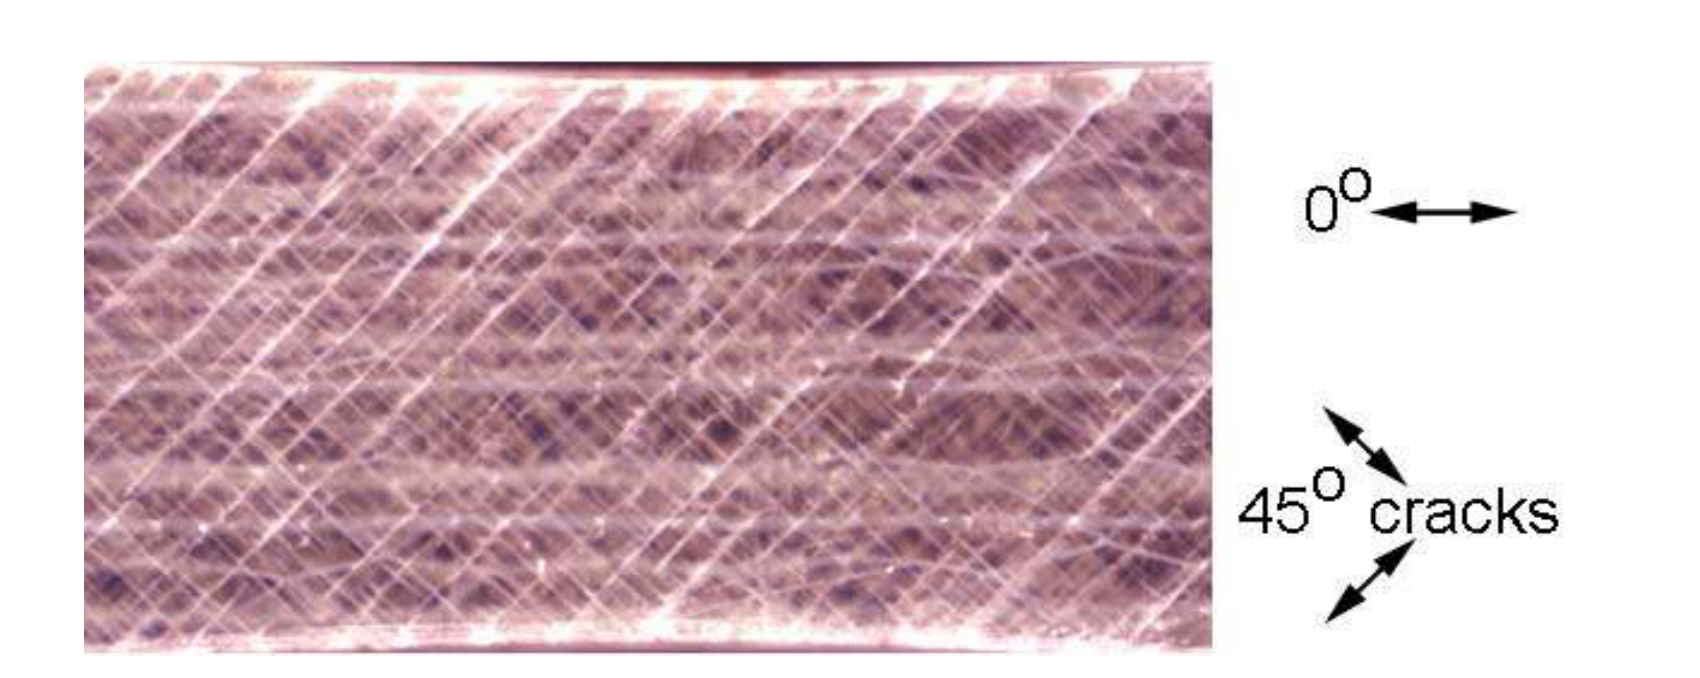
\includegraphics[width=0.75\textwidth]{Figuras/Figuras Antecedentes/grietas_45.png}
    \caption[Agrietamiento de la matriz en capas a $\pm 45^\circ$ antes de la rotura.]{Agrietamiento de la matriz siguiendo la dirección de las fibras en las capas a $\pm 45^\circ$ de un laminado de vidrio, registrado antes de la rotura total de la probeta. La flecha superior indica la dirección de la carga aplicada. Tomado de~\textcite{Samborsky2010}.}
    \label{fig:grietas_45}
\end{figure}

De todos ellos, la delaminación es la que más condiciona la capacidad del laminado, porque se desarrolla entre capas y responde a tensiones interlaminares, cuya evaluación exige representar el laminado capa a capa.

La norma específica de palas traduce esa complejidad en un sistema de factores parciales de material considerablemente más detallado que el de la norma general. Su Sección 6.6.4.2 establece un factor base y lo compone como el producto de una serie de términos que cubren, por separado, el efecto de la temperatura y de la humedad sobre las propiedades, el origen de los datos del material, la validación del cálculo de deformaciones y el número de direcciones de carga consideradas~\parencite{IEC61400-5}. La verificación queda así condicionada no solo por el estado tensional que alcanza la pala, sino también por la calidad de la información disponible sobre el material y sobre el propio modelo de cálculo, aspecto que se retoma al establecer los factores adoptados en este trabajo.

La fragilidad y la ortotropía del laminado explican que la verificación estructural de palas se aborde habitualmente mediante el método de elementos finitos (\gls{fem}). \textcite{HAND2021} lo emplean para verificar la pala compuesta de una \gls{vawt} offshore bajo su caso de carga crítico, contrastando el modelo de elementos finitos con un modelo analítico de viga, y \textcite{Algolfat2022} lo aplican al estudio de la respuesta dinámica de palas de gran escala. El método divide la geometría continua de la pala en un gran número de porciones pequeñas, los elementos, conectadas entre sí en puntos llamados nodos, y supone que dentro de cada elemento los desplazamientos varían según una función sencilla, con lo que el problema continuo, gobernado por ecuaciones diferenciales que no admiten solución analítica en una geometría de esta complejidad, se transforma en un sistema de ecuaciones algebraicas cuyas incógnitas son los desplazamientos nodales. Resuelto ese sistema, se obtienen las deformaciones y, a partir de la ley constitutiva del material, las tensiones en todo el dominio. Dado que la solución es aproximada y mejora al refinar la malla, todo análisis por elementos finitos exige verificar que los resultados ya no dependan significativamente del tamaño de los elementos empleados.

\subsection{Estabilidad estructural y pandeo lineal}
\label{sec:pandeo_teoria}

La resistencia del laminado no agota la verificación estructural. Como se anticipó en la Sección~\ref{sec:analisis-estructural}, la piel de la pala es un cascarón de pared delgada cuyos paneles trabajan en compresión en una de las caras, y un panel comprimido puede perder su forma de equilibrio y abollarse antes de que el material alcance su resistencia. La norma trata esta condición como un estado límite propio, ya que su Sección 7.6.4 exige que las partes portantes de los componentes que no admiten falla no pandeen bajo la carga de diseño, y que ningún componente pandee bajo la carga característica~\parencite{IEC61400-1}.

La carga a la que un panel se vuelve inestable no depende solo del material, sino sobre todo de su geometría. Para una placa comprimida, la tensión crítica sigue la forma de la Ec.~\ref{eq:pandeo_placa}:

\begin{equation}
    \sigma_{cr} = k \, \frac{\pi^2 E}{12\left(1 - \nu^2\right)} \left(\frac{t}{b}\right)^2
    \label{eq:pandeo_placa}
\end{equation}

donde $t$ es el espesor de la placa, $b$ su ancho no apoyado, $E$ el módulo elástico, $\nu$ el coeficiente de Poisson y $k$ un coeficiente que depende de las condiciones de borde y de la relación de aspecto~\parencite{Timoshenko1961}. La dependencia con el cuadrado de la razón $t/b$ explica por qué la estabilidad de la piel se gobierna tanto engrosándola como acortando la distancia entre los elementos que la sostienen, y por qué un rigidizador que no reduce el ancho no apoyado de un panel no mejora su capacidad.

En una geometría real, con paneles de forma irregular y condiciones de borde que no responden a un caso tabulado, la carga crítica se obtiene numéricamente. El planteamiento habitual es el pandeo lineal por autovalores, que parte de la solución estática bajo las cargas aplicadas y busca el factor por el que habría que amplificarlas para que la rigidez del conjunto se anule, según la Ec.~\ref{eq:pandeo_autovalores}:

\begin{equation}
    \left( \left[ K \right] + LM \left[ K_{\sigma} \right] \right) \{\phi\} = \{0\}
    \label{eq:pandeo_autovalores}
\end{equation}

donde $[K]$ es la matriz de rigidez elástica, $[K_{\sigma}]$ la matriz de rigidez geométrica que induce el estado tensional de la solución estática, $\{\phi\}$ el modo de pandeo y $LM$ el multiplicador de carga asociado a ese modo. Un $LM$ mayor que la unidad indica que la estructura no pandea bajo las cargas aplicadas, y su valor mide cuánto margen queda antes de la inestabilidad. El análisis entrega un conjunto de modos ordenados por multiplicador creciente, de los cuales el primero define la condición gobernante. Este enfoque es el que se emplea habitualmente en la verificación de palas de aerogenerador por elementos finitos~\parencite{Boudounit2020,Hameed2015}.

La norma específica de palas admite de forma expresa este planteamiento. Su Sección 6.6.5.6 establece que, cuando la verificación se realiza mediante métodos lineales de análisis de pandeo, debe demostrarse que el autovalor mínimo correspondiente a la primera forma modal supera el factor de seguridad combinado que corresponda~\parencite{IEC61400-5}. Incorpora además una exigencia sobre la discretización que conviene destacar, ya que la idoneidad de la malla ha de acreditarse mediante un estudio de convergencia sobre el propio autovalor de pandeo, y no sobre la tensión, considerándose suficiente cuando aquel no varía más de un $5\%$ al duplicar la densidad de malla en la región pertinente al modo examinado~\parencite{IEC61400-5}. La distinción no es formal, puesto que una malla que ha convergido en tensión puede no haberlo hecho en el autovalor, magnitud considerablemente más sensible a la resolución con que se representa la flexión local del panel.

Conviene retener una limitación del método, ya que la formulación lineal supone que el comportamiento previo a la inestabilidad es elástico y no incorpora imperfecciones geométricas ni la reducción de rigidez que produce el daño progresivo, factores a los que los cascarones de pared delgada son especialmente sensibles. Sus resultados constituyen, por ello, una cota superior de la carga crítica real~\parencite{Timoshenko1961}.

El capítulo siguiente desarrolla el procedimiento con que los elementos revisados, condiciones de viento, simulación aerodinámica y análisis estructural, se aplican al caso de estudio.

\chapter{Metodología}

La metodología de la investigación se estructura en tres etapas principales. En primer lugar, se caracterizan el recurso eólico y las condiciones ambientales del emplazamiento. En segundo lugar, se desarrollan las simulaciones aerodinámicas en QBlade para determinar las solicitaciones actuantes sobre la pala, presentando los parámetros de configuración seleccionados. Finalmente, se ejecuta el análisis estructural por modelo de elementos finitos en a partir de las cargas obtenidas del análisis aerodinámico para cada caso de carga seleccionado.

\section{Geometría del caso de estudio}

Para el desarrollo de los análisis aerodinámicos y estructurales contemplados en esta investigación, se consideran para la turbina las propiedades geométricas presentadas en la Tabla~\ref{tab:geometria_turbina}, proporcionadas por el fabricante de la turbina. El perfil aerodinámico de las palas corresponde al NACA 0018, un perfil simétrico perteneciente a la familia de cuatro dígitos de la National Advisory Committee for Aeronautics (NACA, por sus siglas en ingles). La geometría se presenta en la Figura~\ref{fig:naca0018}.

\begin{figure}[h]
\centering
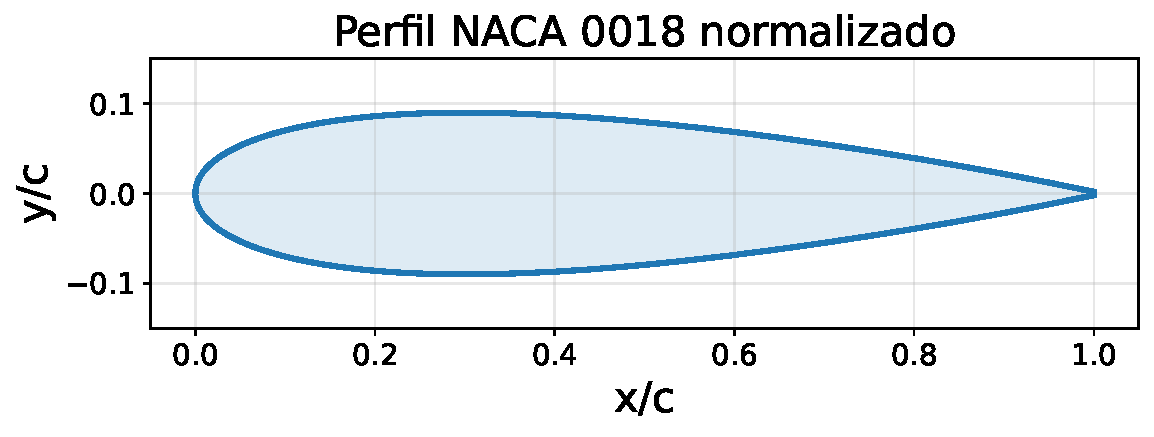
\includegraphics[width=0.7\textwidth, trim=0 0 0 25pt, clip]{Figuras/Figuras Metodología/NACA0018.pdf}
\caption{Perfil NACA 0018 normalizado.}
\label{fig:naca0018}
\end{figure}

\begin{table}[H]
    \caption{Parámetros geométricos del rotor y la pala de la turbina.}
    \label{tab:geometria_turbina}
    \begin{tabular}{lccc}
        \hline
        \textbf{Parámetro Geométrico} & \textbf{Símbolo} & \textbf{Valor} & \textbf{Unidad}\\
        \hline
        Diámetro del rotor                  & $D$     & 20{,}73 & m \\
        Radio del rotor                     & $R$     & 10{,}365 & m \\
        Largo de la pala (Altura del rotor) & $H$     & 23 & m \\
        Longitud de la cuerda de la pala    & $c$     & 1{,}1 & m \\
        Perfil alar                         & —       & NACA 0018   & — \\
        Espesor máximo del perfil           & $t$     & 0{,}198 & m \\
        Número de palas                     & $N$     & 3 & — \\
        Área de barrido del rotor           & $A_s$   & 476{,}79 & m$^2$ \\
        Posición de conexión de struts      & —       & 5{,}0 y 17{,}0 & m \\
        Masa de la pala                     & $m$     & 760 & kg \\
        \hline
    \end{tabular}
\end{table}

\section{Etapa 1: caracterización del emplazamiento y recurso eólico}

\subsection{Caracterización del recurso eólico}
\label{sec:recurso_metodo}

No es posible contar con mediciones anemométricas en el sitio de instalación, ya que por motivos de confidencialidad, no se ha presentado la ubicación exacta de este. En su lugar, se adopta como caso de estudio un emplazamiento representativo de la costa sur de Chile, con coordenadas conocidas (Sección~\ref{sec:sitio_instalacion}), sobre el cual sí es posible aplicar el procedimiento normativo completo; el objetivo es validar la metodología para que pueda reproducirse directamente cuando la ubicación real esté disponible. La caracterización del recurso en ese emplazamiento se apoya en el explorador eólico~\parencite{ExploradorEolico2018}, herramienta desarrollada por el Departamento de Geofísica de la Universidad de Chile mediante un convenio de cooperación con el Ministerio de Energía y el apoyo de la Cooperación Alemana (GIZ) para la evaluación del potencial eólico en el territorio nacional. La serie empleada corresponde a una reconstrucción climatológica de resolución horaria que abarca el periodo entre los años 1980 y 2017. La sección 11.3 de la norma IEC 61400-1~\parencite{IEC61400-1} no fija un número mínimo de años para esta caracterización, sino un mínimo de seis meses de registro, exigiendo además que el periodo sea lo bastante largo para cubrir de forma conservadora las variaciones estacionales; los 37 años de la serie satisfacen ambos requisitos con holgura. La metodología con que el explorador eólico genera y valida estas series se documenta en~\parencite{ExploradorEolico2018,Skamarock2008,Powers2017,Gelaro2017}.

\subsubsection{Caracterización analítica de la velocidad media}

La norma IEC 61400-1~\parencite{IEC61400-1} define la velocidad media anual ($V_{ave}$) como el valor esperado medido sobre una duración suficiente para promediar efectos no estacionarios. Su determinación sigue las etapas siguientes:

\begin{enumerate}
    \renewcommand{\labelenumi}{\alph{enumi})}
    \item \textbf{Ajuste por cizalladura vertical:} Se extrae la serie horaria de la reconstrucción climatológica en el nivel de extracción original ($z = 5{,}5$ m) y se extrapola a la altura del centro del rotor ($z = 21{,}3$ m) aplicando el perfil de viento normal (\gls{nwp}) descrito en la Sección~\ref{sec:condiciones_diseno} mediante la Ec.~\ref{eq:nwp_ley_potencia}, con el exponente de cizalladura $\alpha_z = 0{,}12$ adoptado para el emplazamiento offshore.

    \item \textbf{Cálculo de la media aritmética:} Sobre la serie ya extrapolada a la altura del centro del rotor, se calcula la media mediante la Ec.~\ref{eq:media_aritmetica}:
    \begin{equation}
        V_{ave} = \frac{1}{N} \sum_{i=1}^{N} V_i
        \label{eq:media_aritmetica}
    \end{equation}
    donde $V_i$ es cada uno de los $N$ registros horarios de velocidad de la serie extrapolada.

    \item \textbf{Velocidad de referencia:} A partir de la velocidad media anual ya extrapolada a la altura del centro del rotor ($V_{ave}$ a $z = 21{,}3$ m), se determina la velocidad de referencia ($V_{ref}$) definida en la Sección 6.3.1.1 de la norma IEC 61400-1~\parencite{IEC61400-1} para la clasificación de emplazamientos, según la Ec.~\ref{eq:vave_vref}:
    \begin{equation}
        V_{ave} = 0{,}2 \, V_{ref}
        \label{eq:vave_vref}
    \end{equation}

    \item \textbf{Modelado de la distribución de probabilidad:} Sobre la serie ya extrapolada a la altura del centro del rotor, la distribución de probabilidad de frecuencias ($f_W$) de la velocidad del viento se modela mediante la distribución de Weibull descrita en la Sección~\ref{sec:distribucion_viento}, cuyo ajuste permite describir la permanencia del viento en el emplazamiento. Al tratarse de una evaluación sitio-específica sobre un registro histórico, y no de la adopción de una clase estándar, ambos parámetros se ajustan por máxima verosimilitud~\parencite{Seguro2000}, en lugar de fijar $k = 2$ como en el modelo de Rayleigh de referencia. La función de densidad de probabilidad se expresa según la Ec.~\ref{eq:weibull_pdf_general}:
    \begin{equation}
        f_W(V; k, c) = \frac{k}{c} \left( \frac{V}{c} \right)^{k-1} \exp\left[ -\left( \frac{V}{c} \right)^k \right]
    \label{eq:weibull_pdf_general}
    \end{equation}
    donde $k$ es el parámetro de forma (adimensional) y $c$ el parámetro de escala (m/s), ambos determinados a la altura del centro del rotor. La estimación por máxima verosimilitud sobre los $N$ registros $V_i$ de la serie resuelve primero el parámetro de forma como raíz de la Ec.~\ref{eq:weibull_mle_k}, que no admite solución explícita y se obtiene por iteración numérica:
    \begin{equation}
        \frac{\sum_{i=1}^{N} V_i^{\,k} \ln V_i}{\sum_{i=1}^{N} V_i^{\,k}} - \frac{1}{k} - \frac{1}{N} \sum_{i=1}^{N} \ln V_i = 0
        \label{eq:weibull_mle_k}
    \end{equation}
    y a partir de ese valor obtiene el parámetro de escala por sustitución directa, según la Ec.~\ref{eq:weibull_mle_c}:
    \begin{equation}
        c = \left( \frac{1}{N} \sum_{i=1}^{N} V_i^{\,k} \right)^{1/k}
        \label{eq:weibull_mle_c}
    \end{equation}
\end{enumerate}

\subsubsection{Caracterización de la turbulencia según IEC 61400-3}
\label{sec:ntm}

Para caracterizar la turbulencia del flujo incidente se aplica el modelo de turbulencia normal (NTM) que la norma IEC 61400-3~\parencite{IEC61400-3} adopta para emplazamientos offshore, y cuya formulación se recoge en la Ec.~\ref{eq:ntm_sigma} de la Sección~\ref{sec:condiciones_diseno}. Esa expresión queda definida por dos parámetros, la intensidad de turbulencia de referencia $I_{ref}$ y el parámetro de ordenada $b_{NTM}$, que la norma tabula según la categoría de turbulencia asignada al emplazamiento~\parencite{IEC61400-1}.

La Sección 12.3 de IEC 61400-3~\parencite{IEC61400-3} establece que, a falta de datos de turbulencia del emplazamiento, la desviación estándar de la velocidad puede estimarse a partir de la rugosidad de la superficie del mar. Esa rugosidad no es un valor fijo, sino que crece con la velocidad del viento, porque es el propio viento el que levanta el oleaje que la produce. La norma recoge ese acoplamiento mediante la relación de \textcite{Charnock1955}, que vincula la longitud de rugosidad con la velocidad de fricción del flujo, según la Ec.~\ref{eq:charnock_z0}:

\begin{equation}
    z_0 = \frac{A_C}{g} \left[ \frac{\kappa \, V_{hub}}{\ln \left( z_{hub} / z_0 \right)} \right]^2
    \label{eq:charnock_z0}
\end{equation}

donde $z_0$ es la longitud de rugosidad de la superficie del mar (medida en metros), $g$ la aceleración de gravedad, la constante de von Kármán $\kappa = 0{,}4$ y la constante de Charnock $A_C$, que la norma fija en $0{,}011$ para mar abierto~\parencite{IEC61400-3}. La expresión es implícita, ya que $z_0$ aparece en ambos miembros, y se resuelve por iteración numérica. Con la rugosidad así obtenida, la desviación estándar representativa se calcula según la Ec.~\ref{eq:charnock_sigma}:

\begin{equation}
    \sigma_{NTM} = \frac{V_{hub}}{\ln \left( z_{hub} / z_0 \right)} + 1{,}28 \cdot 1{,}44 \cdot I_{ref}
    \label{eq:charnock_sigma}
\end{equation}

donde $I_{ref}$ interviene evaluado a $V_{hub} = 15$~m/s, ya que la norma lo define precisamente como el valor esperado de la intensidad de turbulencia a esa velocidad~\parencite{IEC61400-1}. Conviene precisar que esta velocidad de $15$~m/s es un punto fijo de la norma IEC 61400-1.

\subsubsection{Generación del campo de viento turbulento}
\label{sec:campo_turbulento}

Para la simulación aerodinámica en QBlade, el campo de viento incidente se genera mediante el modelo de Mann descrito en la Sección~\ref{sec:modelo_mann}, con los parámetros de turbulencia de la categoría asignada al emplazamiento (Sección~\ref{sec:ntm}). El modelo no sintetiza el viento sobre la turbina, sino sobre un volumen de aire que después se hace pasar por ella. Ese volumen es la caja de turbulencia: un prisma de velocidades fluctuantes almacenadas sobre una grilla regular de puntos, con dos direcciones transversales al flujo, que deben cubrir el plano barrido por el rotor. La Figura~\ref{fig:caja_turbulencia} ilustra la caja sintetizada para una de las realizaciones simuladas, con la turbina superpuesta a escala para dimensionar el volumen de aire generado frente al rotor.

\begin{figure}[H]
    \centering
    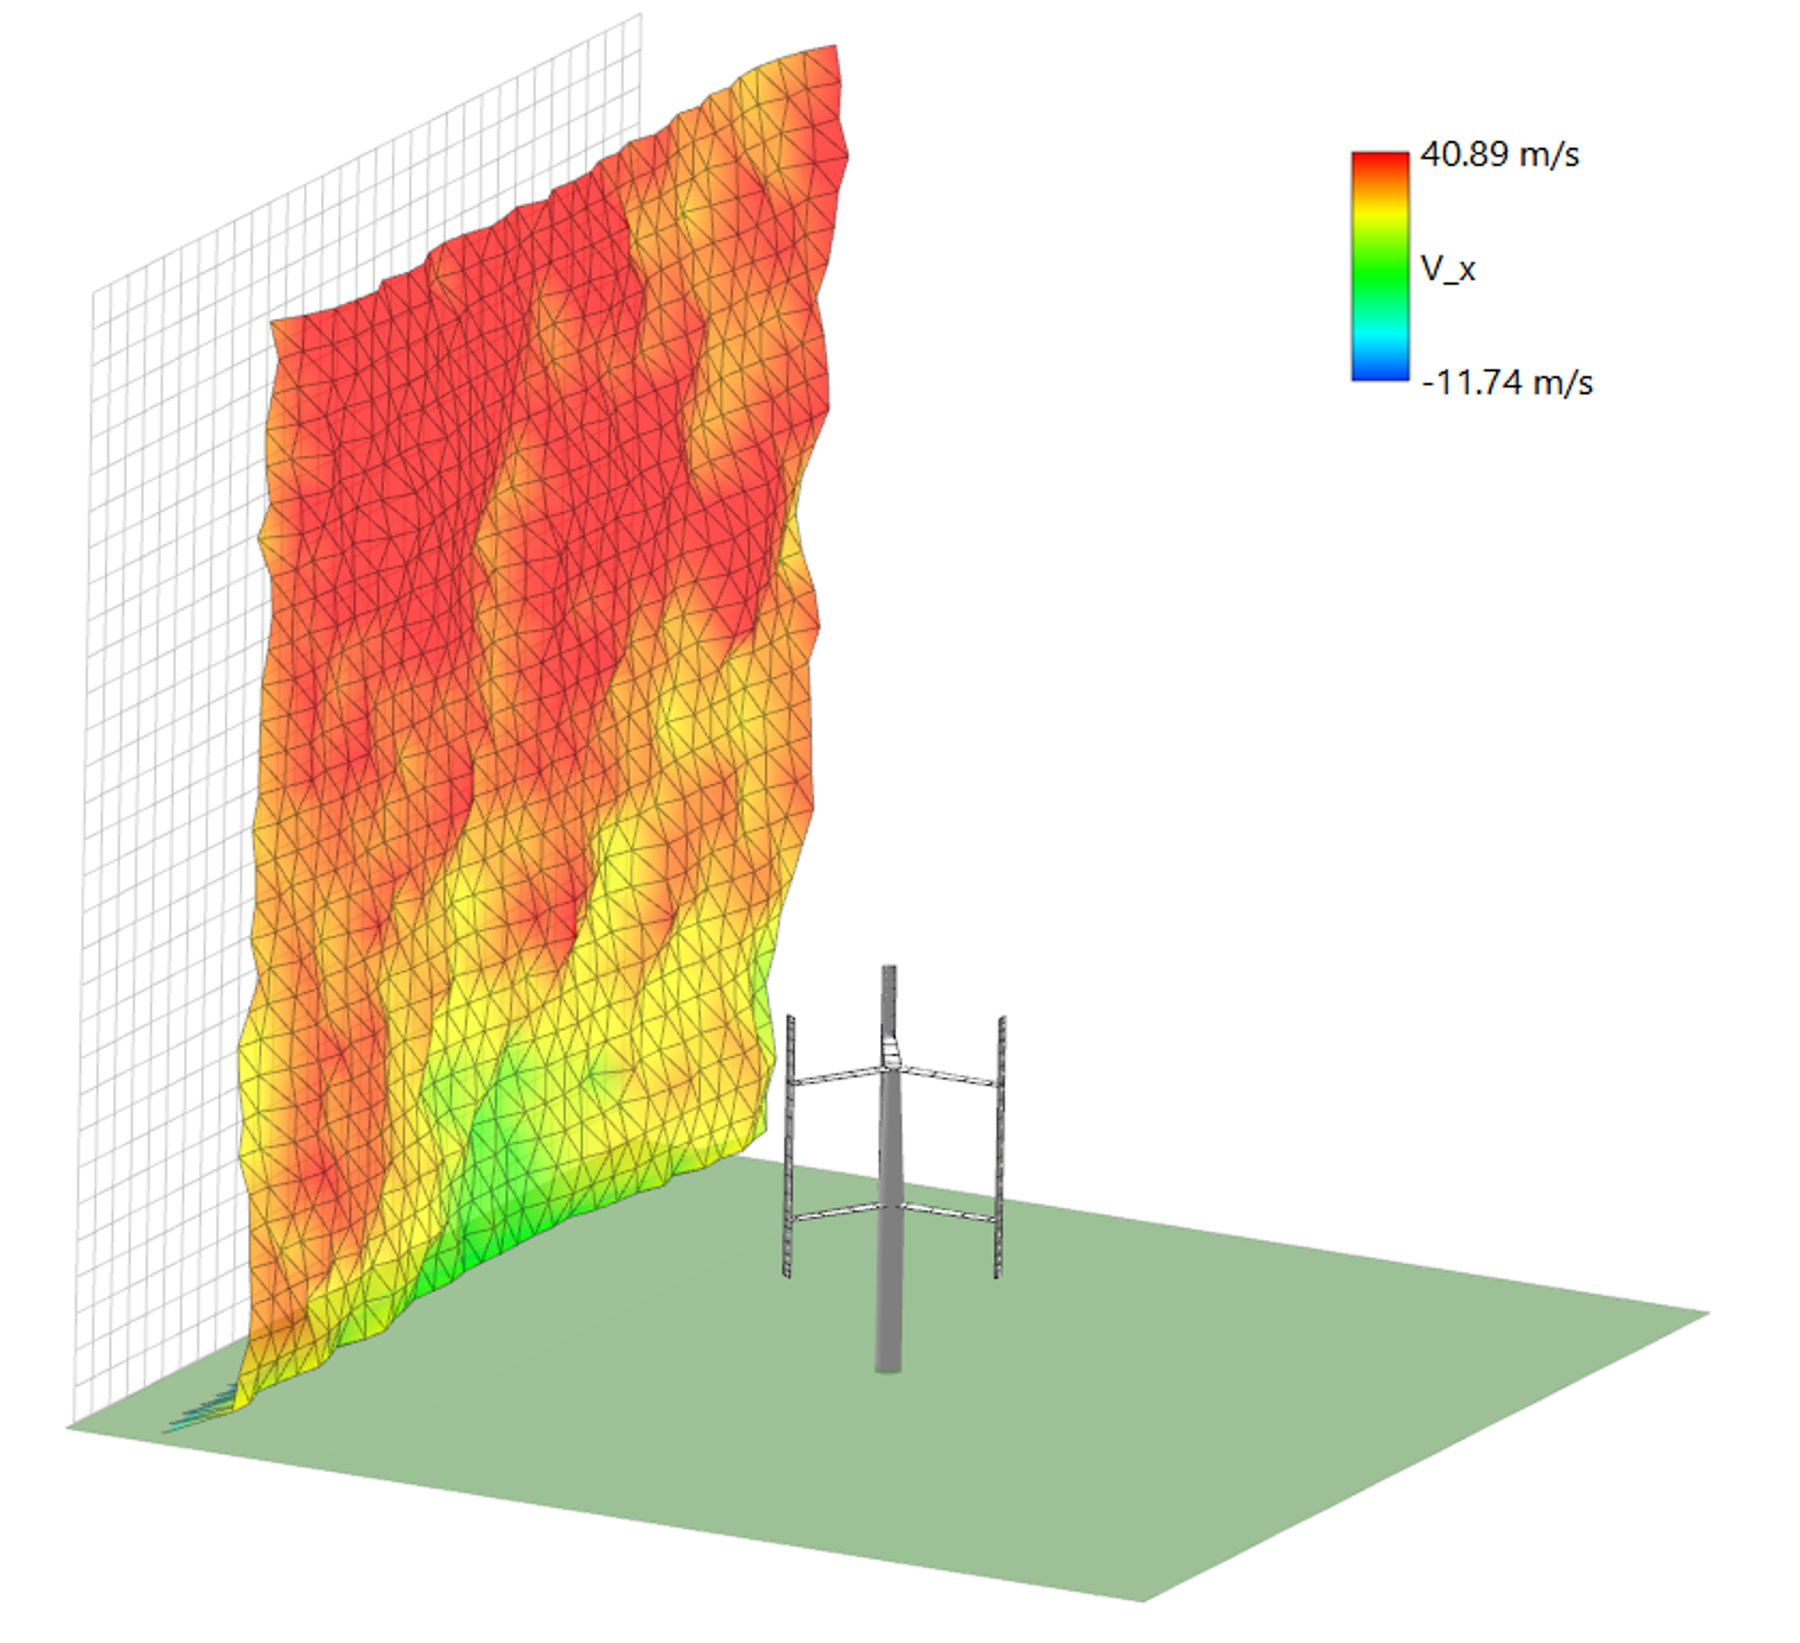
\includegraphics[width=0.7\textwidth]{Figuras/caja_turbulencia_3d.png}
    \caption[Caja de turbulencia generada por el modelo de Mann.]{Caja de turbulencia sintetizada por el modelo de Mann para una de las realizaciones simuladas, coloreada según la componente longitudinal de la velocidad ($V_x$), con la turbina superpuesta a escala.}
    \label{fig:caja_turbulencia}
\end{figure}

La sección transversal se dimensiona en $100 \times 100$~m, discretizada en $32 \times 32$ puntos, configuración empleada por Marten en sus estudios de validación del software~\parencite{marten2019qblade}. La longitud no se fija de forma independiente, ya que resulta del producto de la velocidad media del caso por la duración de la simulación.

Las dimensiones adoptadas satisfacen los requisitos aplicables de IEC 61400-1~\parencite{IEC61400-1} en dos aspectos. Por una parte, la sección transversal cubre íntegramente el plano barrido por el rotor, de $D = 20{,}73$~m de ancho y $H = 23$~m de extensión vertical: ese plano ocupa $476{,}79$~m$^2$ de los $10\,000$~m$^2$ de la sección de la caja, esto es, un $4{,}8\%$ de su área, con un dominio casi cinco veces más ancho que el rotor y más de cuatro veces más alto. El dominio cubre así el plano barrido con holgura, condición necesaria para el muestreo rotacional que la Sección 6.3 de la norma IEC 61400-1~\parencite{IEC61400-1} exige admitir al modelo de turbulencia, ya que la pala describe una trayectoria circular y en cada instante interroga puntos distintos de la grilla. Por otra parte, el Anexo B de la norma IEC 61400-1~\parencite{IEC61400-1} recomienda ajustar la factorización del tensor espectral del modelo de Mann cuando el dominio espacial es inferior a $8\ell$ en alguna de sus dimensiones, donde $\ell$ es la escala de longitud del modelo, definida en la Sección~\ref{sec:modelo_mann} como $\ell = 0{,}8\,\Lambda_1$, siendo $\Lambda_1 = 0{,}7\,z = 14{,}9$~m el parámetro de escala de turbulencia longitudinal para la altura del centro del rotor ($z = 21{,}3$~m $< 60$~m, Ecuación 5 de la norma IEC 61400-1~\parencite{IEC61400-1}). El umbral resultante, $8\ell \approx 95{,}4$~m, es inferior a los $100$~m de la caja empleada, por lo que no se requiere dicho ajuste.

La resolución de la grilla se contrasta con esa misma escala. El espaciamiento transversal es de $3{,}23$~m, resultado de repartir los $100$~m de ancho entre los $31$ intervalos de la grilla, y el longitudinal, igual al producto de la velocidad por el paso temporal, alcanza $2{,}4$~m en el caso más rápido. La escala $\ell$ equivale por tanto a casi cuatro veces el espaciamiento transversal y a unas cinco veces el longitudinal, de modo que un remolino del tamaño que concentra la energía del campo queda descrito por varios puntos de la grilla y no por uno solo. Las estructuras menores que el espaciamiento no se resuelven, y su energía se repone mediante la compensación de altas frecuencias que se describe más adelante.

La Figura~\ref{fig:mann_config} reproduce la ventana con que se configura cada caja en QBlade, ilustrada para la velocidad de $24$~m/s. Sus campos se agrupan en cuatro bloques, que se describen a continuación. Los valores numéricos de la caracterización del emplazamiento que alimentan esta ventana se reportan en el Capítulo~4.

\begin{figure}[H]
    \centering
    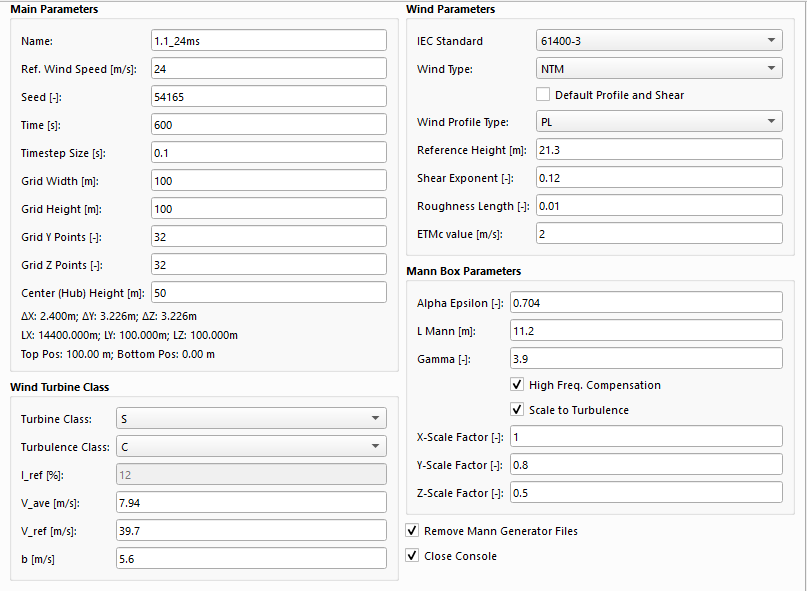
\includegraphics[width=0.7\textwidth]{Figuras/Mann.png}
    \caption[Configuración del modelo de Mann en QBlade.]{Configuración del modelo de Mann para la generación del campo de viento turbulento en QBlade, ilustrada para la velocidad de $24$~m/s.}
    \label{fig:mann_config}
\end{figure}

\textbf{Parámetros principales.} Definen la geometría de la caja y su discretización. La velocidad de referencia es la del centro del rotor del caso de carga que se simula, y la semilla es el entero que inicializa el generador de números aleatorios, distinto en cada una de las seis realizaciones de cada velocidad (Sección~\ref{sec:velocidades_simulacion}), que es lo que hace que representen realizaciones independientes del mismo proceso estocástico. La duración de $600$~s y el paso temporal de $0{,}1$~s fijan, junto con la velocidad, la longitud del dominio longitudinal y su resolución. Los campos de ancho, alto y número de puntos son los ya justificados. La altura del centro de la caja se fija en $50$~m, y no en la del centro del rotor, de modo que el dominio abarca desde el nivel del mar hasta los $100$~m, cotas que la propia ventana informa: es una posición de la caja en el espacio, no un dato de la turbina, que se declara aparte como altura de referencia.

\textbf{Clase de turbina.} La turbina se declara de clase S, denominación que la norma reserva para los emplazamientos cuyas condiciones no quedan descritas por una clase estándar~\parencite{IEC61400-1}, ya que la velocidad media y la velocidad de referencia provienen del registro del sitio (Sección~\ref{sec:recurso_metodo}) y no de los valores tabulados. La turbulencia, en cambio, se declara en la categoría asignada en la Sección~\ref{sec:ntm}, con lo que el programa toma para ella los valores que la norma tabula. Los cuatro campos que siguen recogen esa combinación: la velocidad media y la velocidad de referencia obtenidas de la caracterización del recurso, y la intensidad de turbulencia de referencia y el parámetro de ordenada propios de la categoría adoptada.

\textbf{Parámetros de viento.} Fijan el marco normativo y el perfil medio sobre el que se superpone la turbulencia. Se selecciona la norma IEC 61400-3~\parencite{IEC61400-3} por tratarse de un emplazamiento marino, y el tipo de viento es el modelo de turbulencia normal para los DLC 1.1 y 1.2; el DLC 1.3 emplea en su lugar el modelo de turbulencia extrema, cuya constante $c_{ETM} = 2$~m/s, fijada en la Sección 6.3.2.3 de la norma IEC 61400-1~\parencite{IEC61400-1}, es la que recoge el campo correspondiente. La casilla de perfil y cizalladura por defecto se deja sin marcar precisamente para introducir los valores del emplazamiento en lugar de los tabulados: el perfil se declara como ley de potencia, que es la forma que la norma da al perfil de viento normal (Sección~\ref{sec:condiciones_diseno}), con la altura de referencia del centro del rotor y el exponente de cizalladura adoptado para el sitio, los mismos con que se extrapoló la serie de viento. La longitud de rugosidad es el parámetro que gobierna el perfil logarítmico, la alternativa al de ley de potencia adoptado aquí.

\textbf{Parámetros de la caja de Mann.} Corresponden a los tres del tensor espectral descritos en la Sección~\ref{sec:modelo_mann}: el parámetro de intensidad, bajo la denominación \textit{Alpha Epsilon}, que se obtiene de la desviación estándar representativa mediante $\sigma_{iso} = 0{,}55\,\sigma_{NTM}$ y que por ello cambia con cada velocidad simulada; la escala de longitud $\ell$, bajo la denominación \textit{L Mann}; y el parámetro de anisotropía \textit{Gamma}, que la norma fija en $3{,}9$. Los factores de escala en las tres direcciones, $1$, $0{,}8$ y $0{,}5$, reproducen las razones entre las desviaciones estándar de las tres componentes de la velocidad que la norma tabula en su Anexo B, $\sigma_2 = 0{,}8\,\sigma_1$ y $\sigma_3 = 0{,}5\,\sigma_1$. Las dos casillas activadas actúan sobre la energía del campo generado. Como la síntesis se resuelve por transformada de Fourier sobre los números de onda que la grilla contiene, según se detalla en el mismo Anexo B, los mayores que su resolución quedan fuera del campo: a reponer esa fracción de energía apunta la compensación de altas frecuencias. El escalado a la turbulencia, por su parte, ajusta el campo sintetizado para que su desviación estándar coincida con la prescrita. Las dos casillas restantes gobiernan el manejo de los archivos temporales del generador y no tienen efecto sobre el campo.

\subsection{Determinación de las propiedades termofísicas del aire}
\label{sec:propiedades_aire}

La norma IEC 61400-1~\parencite{IEC61400-1} incluye la temperatura y la densidad del aire entre las condiciones ambientales que deben evaluarse para el emplazamiento (Secciones 6.4 y 11.1), y el método aerodinámico las requiere de forma explícita: la densidad escala las fuerzas que actúan sobre la pala, y la viscosidad cinemática fija el número de Reynolds con el que se interpolan las polares del perfil durante la simulación~\parencite{marten2019qblade}. Ese número de Reynolds condiciona el resultado aerodinámico, porque las polares varían con él de forma apreciable dentro del rango en que opera la turbina, según se expone en la Sección~\ref{sec:polares}. Adoptar las propiedades de la atmósfera estándar, definidas a $15$~\textdegree C~\parencite{Anderson2016}, desplazaría por tanto el rango de Reynolds del cálculo respecto del que la pala experimenta en un emplazamiento cuya temperatura media difiere de ese valor. Por esta razón las propiedades se determinan a partir de la climatología mensual del sitio (Capítulo~4) mediante las correlaciones analíticas de uso establecido en la literatura aerodinámica para evaluar las propiedades de transporte de un gas en función de su temperatura~\parencite{White2006,Anderson2016}, en lugar de tomarse de una tabla a temperatura fija.

La viscosidad dinámica se calcula mediante la ley de Sutherland~\parencite{Sutherland1893}, correlación de referencia para la dependencia de la viscosidad de un gas con la temperatura y de uso estándar para el aire~\parencite{White2006}, según la Ec.~\ref{eq:sutherland}:

\begin{equation}
    \mu = \mu_0 \frac{T_0 + C}{T + C} \left( \frac{T}{T_0} \right)^{3/2}
    \label{eq:sutherland}
\end{equation}

donde $T$ es la temperatura del aire, $\mu_0 = 1{,}7894 \times 10^{-5}$ kg/(m·s) y $T_0 = 288{,}16$ K son la viscosidad y la temperatura del aire en las condiciones de la atmósfera estándar a nivel del mar~\parencite{Anderson2016}, par que constituye el punto de referencia de la correlación, y $C = 110{,}4$ K es la constante de Sutherland para el aire~\parencite{White2006}.

La densidad del aire se calcula mediante la ecuación de estado de los gases ideales~\parencite{Anderson2016}, aplicable al aire en el rango de presiones y temperaturas del emplazamiento, con $P_{atm} = 101325$ Pa ($1$ atm), valor de la presión atmosférica a nivel del mar según la atmósfera estándar~\parencite{Anderson2016}, de acuerdo con la Ec.~\ref{eq:densidad_aire}:

\begin{equation}
    \rho = \frac{P_{atm}}{R_a \cdot T}
    \label{eq:densidad_aire}
\end{equation}

donde $R_a = 287{,}05$ J/(kg·K) es la constante del gas para el aire seco~\parencite{Anderson2016}.

Ambas propiedades se combinan en la viscosidad cinemática, magnitud que interviene en el número de Reynolds y que se define como el cociente entre la viscosidad dinámica y la densidad~\parencite{White2006}, según la Ec.~\ref{eq:visc_cinematica}:

\begin{equation}
    \nu = \frac{\mu}{\rho}
    \label{eq:visc_cinematica}
\end{equation}

donde $\mu$ es la viscosidad dinámica obtenida de la Ec.~\ref{eq:sutherland} y $\rho$ la densidad de la Ec.~\ref{eq:densidad_aire}, ambas evaluadas a la temperatura media del emplazamiento. El valor resultante se presenta en el Capítulo~4.


\section{Etapa 2: modelado aerodinámico}

De las familias de métodos aerodinámicos comparadas en la Tabla~\ref{tab:comparacion_metodos}, se adopta el método de línea sustentadora con estela de vórtice libre (\gls{llfvw}), implementado en el software QBlade~\parencite{marten2019qblade}. El criterio de selección responde a las exigencias de la verificación normativa: los casos de carga requieren $72$ realizaciones de varios minutos con acoplamiento aeroelástico, volumen incompatible con el costo del CFD, mientras que el carácter inestable del flujo en un H-rotor y la interacción de la pala con su propia estela quedan fuera del alcance del DMST. El modelo DMST se reserva, por su bajo costo, para la estimación preliminar del \gls{tsr} óptimo (Sección~\ref{sec:dmst}), que sirve de punto de partida para las simulaciones LLFVW.

Tanto QBlade como el método empleado se apoyan en polares que describen las cargas sobre el perfil, y esas polares deben cubrir todo el rango de funcionamiento de la turbina. Como el fabricante no proporciona los parámetros operacionales, dicho rango se determina en los pasos que siguen.

\subsection{Determinación del rango operativo del número de Reynolds}
\label{sec:reynolds}

Debido a la cinemática de las \gls{vawt}, el perfil alar experimenta una velocidad relativa variable según su posición en la trayectoria circular, por lo que el número de Reynolds también varía durante la operación. Para determinar el intervalo operativo utilizado en el cálculo de polares, se evalúa la velocidad relativa $W$ en función del ángulo azimutal $\theta$, según la Ec.~\ref{eq:W_theta}:

\begin{equation}
    W(\theta) = V_{hub} \sqrt{1 + 2\lambda \cos\theta + \lambda^2}
    \label{eq:W_theta}
\end{equation}

donde $V_{hub}$ es la velocidad del viento a la altura del centro del rotor y $\lambda$ la relación de velocidad de punta. Los valores extremos de $W$ ocurren en las posiciones de barlovento ($\theta = 0^\circ$) y sotavento ($\theta = 180^\circ$), donde la expresión se simplifica según las Ecs.~\ref{eq:W_max} y~\ref{eq:W_min}:

\begin{equation}
    W_{max} = V_{hub} + \Omega R
    \label{eq:W_max}
\end{equation}

\begin{equation}
    W_{min} = |V_{hub} - \Omega R|
    \label{eq:W_min}
\end{equation}


La condición operacional más exigente para el perfil corresponde a la velocidad de corte $V_{out}$ con el rotor girando a su velocidad máxima, resultando una velocidad relativa máxima $W_{max}$. A partir de la cuerda del perfil y la viscosidad cinemática, el número de Reynolds se calcula según la Ec.~\ref{eq:Re_max_theoretical}:

\begin{equation}
    Re_{max} = \frac{W_{max} \cdot c}{\bar{\nu}}
    \label{eq:Re_max_theoretical}
\end{equation}

donde $\bar{\nu}$ es la viscosidad cinemática media del aire en el emplazamiento, obtenida según el procedimiento de la Sección~\ref{sec:propiedades_aire} y reportada en el Capítulo~4. Este valor constituye una referencia determinística para el régimen de producción de potencia, ya que la turbina se desconecta para $V > V_{out}$; las fluctuaciones turbulentas instantáneas pueden excederlo transitoriamente. Ese valor, redondeado al millón siguiente, define el límite superior del cálculo de polares. El rango paramétrico $\lambda \in [2{,}5; 4{,}5]$ y $V \in [2; 25]$~m/s constituye una envolvente teórica preliminar que abarca todas las combinaciones posibles de \gls{tsr} y velocidad de viento. El intervalo de $\lambda$ queda contenido en el documentado para las configuraciones H-Darrieus (Tabla~\ref{tab:tabla_vawt}), y el de velocidades corresponde al rango operacional adoptado en la Sección~\ref{sec:control}. El número de Reynolds operacional, verificado mediante las simulaciones \gls{llfvw}, se presenta en el Capítulo~4.

Una vez definido el rango de Reynolds, se procede al cálculo de las curvas polares mediante la siguiente estrategia de discretización, resumida en la Tabla~\ref{tab:reynolds_discretizacion}.

\begin{table}[H]
    \centering
    \caption{Estrategia de discretización del número de Reynolds para el cálculo de polares.}
    \label{tab:reynolds_discretizacion}
    \begin{tabular}{lcc}
        \hline
        \textbf{Rango} & $\Delta Re$ & \textbf{Fuente} \\
        \hline
        $60$k -- $300$k & --- & \cite{Bianchini2015} \\
        $350$k -- $1$M & $50\,000$ & QFoil \\
        $1$M -- $3$M   & $125\,000$ & QFoil \\
        $3$M -- $6$M   & $250\,000$ & QFoil \\
        \hline
    \end{tabular}
\end{table}

El cálculo con QFoil se inicia en $Re = 3{,}5 \times 10^5$, ya que por debajo de $Re = 2{,}5 \times 10^5$ no se alcanza la convergencia numérica del solucionador. Se decide cubrir el rango inferior con las polares experimentales de \textcite{Bianchini2015} para el perfil NACA 0018 ($Re = 0{,}6$; $1{,}5$; $2{,}5$ y $3{,}0 \times 10^5$), digitalizadas de las mediciones en túnel de viento publicadas e ingresadas a QBlade como tablas de puntos de $C_l$ y $C_d$ frente al ángulo de ataque, en el mismo formato con que el programa recibe las calculadas. Recurrir a esa fuente mantiene la coherencia del conjunto, porque es la misma contra la que se resuelven el criterio de transición (Sección~\ref{sec:calculo_polares}) y los parámetros del modelo de extrapolación (Sección~\ref{sec:extrapolacion_polares}): las polares de bajo Reynolds no son un dato ajeno añadido al margen, sino el patrón de contraste con el que se calibra el resto del conjunto.


\subsection{Cálculo de polares}
\label{sec:calculo_polares}

Se calculan las curvas polares mediante QFoil, preferible a XFoil en el régimen de pérdida profunda propio de una \gls{vawt} por las razones expuestas en la Sección~\ref{sec:polares}. Se utilizan los siguientes parámetros de configuración:

\begin{itemize}
    \item \textbf{Número de Mach:} La velocidad relativa máxima del rotor (Sección~\ref{sec:reynolds}), contrastada con la velocidad del sonido evaluada a la temperatura mínima del emplazamiento, arroja un número de Mach máximo del orden de $0{,}2$, muy por debajo del umbral de $0{,}3$ bajo el cual la variación de densidad sobre el perfil es despreciable (Sección~\ref{sec:polares}). El flujo admite por tanto tratarse como incompresible en todo el rango operacional, y el valor de Mach se fija en $0$ para que el solucionador prescinda de la corrección de compresibilidad de Kármán-Tsien~\parencite{Karman1941,Tsien1939}, cuya aplicación no aportaría precisión y sí introduciría una fuente adicional de error en el cálculo de las polares.

    \item \textbf{Criterio de transición ($N_{crit}$):} Las curvas polares se calculan para seis valores de $N_{crit}$: $4$, $6$, $7$, $9$, $11$ y $12$. Los valores se seleccionan a partir del valor de referencia de túnel de viento promedio ($N_{crit}=9$), explorando valores menores para representar entornos de mayor turbulencia y valores superiores para condiciones de flujo más limpio, conforme a los rangos descritos en la Tabla~\ref{tab:ncrit_values}. El valor adoptado para las simulaciones se resuelve comparando las seis polares con los datos experimentales de \textcite{Bianchini2015} a $Re = 2{,}5 \times 10^5$, y se presenta en el Capítulo~4.
    
    \item \textbf{Transición de capa límite:} Los parámetros \textit{Forced Top Transition} y \textit{Forced Bottom Transition} se fijan en $1{,}0$, permitiendo que el modelo de transición natural actúe a lo largo de toda la cuerda del perfil.

    \item \textbf{Panelado del perfil:} Se ajusta el panelado del perfil a 220 paneles con distribución de coseno~\parencite{drela1989xfoil}.
\end{itemize}

\subsection{Metodología de extrapolación de polares}
\label{sec:extrapolacion_polares}

Para simular el rendimiento del rotor de eje vertical (\gls{vawt}), se implementa el modelo de \textcite{montgomerie2004methods} en QBlade. La determinación de los parámetros del modelo se basa en los siguientes criterios:

\textbf{Determinación del coeficiente de arrastre a 90° ($C_{d90}$):} El parámetro $C_{d90}$ define la amplitud de las curvas en régimen de pérdida profunda. Su valor se determina a partir de los datos experimentales en túnel de viento de \textcite{Bianchini2015} para el perfil NACA 0018 a $Re = 2{,}5 \times 10^5$, y se reporta en el Capítulo~4.

\textbf{Determinación de la pendiente de sustentación:} La pendiente de la parte lineal de la curva de sustentación es calculada automáticamente por QBlade mediante un ajuste lineal de mínimos cuadrados de primer orden sobre el intervalo de las soluciones de QFoil comprendido entre $\alpha = -5^\circ$ y $\alpha = 5^\circ$~\parencite{marten2019qblade}.

\textbf{Configuración de los parámetros de acoplamiento ($A$ y $B$):} Estos coeficientes adimensionales controlan la forma y la suavidad de la curva extrapolada en los rangos de transición hacia el comportamiento de placa plana. Para perfiles simétricos, los valores positivos y negativos se configuran con idéntico valor absoluto ($A+ = A-$ y $B+ = B-$) para mantener la consistencia física. Su ajuste se realiza de manera visual en QBlade, tomando como referencia los datos experimentales de \textcite{Bianchini2015}, con el criterio de lograr una transición asintótica y libre de discontinuidades inmediatamente después del punto de pérdida original de QFoil.

\subsection{Estimación preliminar del TSR óptimo mediante DMST}
\label{sec:dmst}

Como paso previo a las simulaciones de alta fidelidad con \gls{llfvw}, se emplea el \gls{dmst}, descrito en la Sección~\ref{sec:metodos_aerodinamicos}, para obtener una primera estimación del \gls{tsr} óptimo de la turbina. La simulación se configura con el modelo de pérdida de punta activado, ya que, el \gls{dmst}, al representar el rotor mediante tubos de corriente bidimensionales independientes, el método asume implícitamente una pala de envergadura infinita y no reproduce por sí solo la pérdida de sustentación hacia la punta, producida por los vórtices que allí se desprenden~\parencite{marten2019qblade}. La pala se discretiza en $50$ elementos, y las propiedades del fluido se calculan a partir del análisis de viento y temperatura del emplazamiento. El barrido se ejecuta sobre un rango de velocidades de viento de $2$ a $25$ m/s con incrementos de $0{,}1$ m/s y velocidad de rotación $\Omega$ de $3$ a $42$ rpm con incrementos de $0{,}1$ rpm. De cada combinación $(V, \Omega)$ se obtiene el \gls{tsr} como $\lambda = \Omega R / V$. El \gls{tsr} correspondiente al máximo $C_p$ de cada curva proporciona el valor de referencia para configurar las simulaciones aerodinámicas posteriores.

\subsection{Definición de la turbina en QBlade}

\subsubsection{Discretización e instrumentación de la pala}
\label{sec:discretizacion}

La definición de la turbina en QBlade requiere establecer dos esquemas de discretización independientes para la pala: uno aerodinámico, que gobierna la resolución del método de vórtices libres, y uno que fija las estaciones donde se instrumenta la pala para extraer las fuerzas aerodinámicas.

\textbf{Panelado aerodinámico:} Para la resolución del método \gls{llfvw}, la pala se divide en 21 paneles con distribución de tipo coseno, que reduce el tamaño de los paneles hacia la punta de la pala para capturar mejor los mayores gradientes de circulación que ahí se presentan, configuración con la que \textcite{marten2019qblade} valida el método en QBlade; la documentación del software describe las configuraciones alternativas disponibles~\parencite{QBladeDocs2024}. Entre paneles contiguos, la circulación se interpola mediante splines cúbicos de clase C2, polinomios que empalman sin discontinuidades hasta su segunda derivada. La Figura~\ref{fig:panelado_aerodinamico} muestra la distribución resultante sobre las tres palas del rotor.

\begin{figure}[H]
\centering
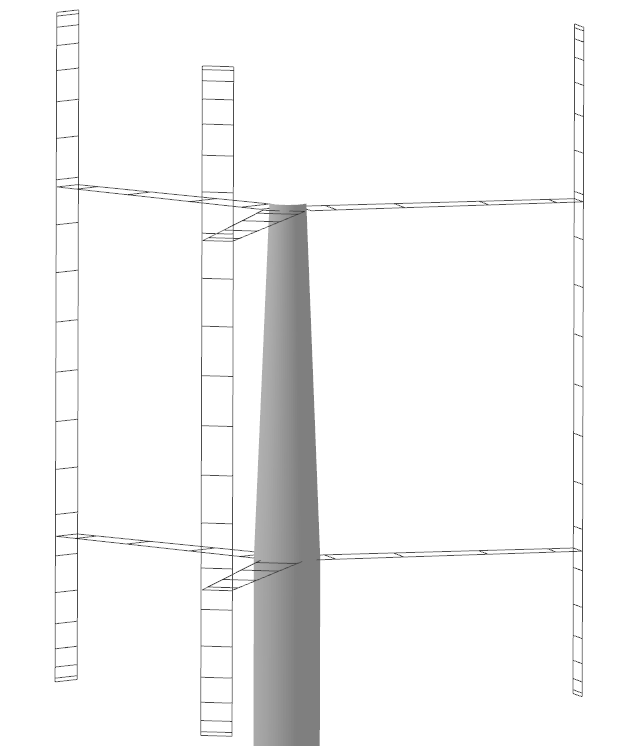
\includegraphics[width=0.55\textwidth]{Figuras/Figuras Metodología/panelado_aerodinamico.png}
\caption[Panelado aerodinámico del rotor en QBlade.]{Panelado aerodinámico de las tres palas del rotor en QBlade, según la distribución de tipo coseno descrita en el texto.}
\label{fig:panelado_aerodinamico}
\end{figure}

\textbf{Estaciones de extracción de cargas:} La pala se discretiza en 23 elementos uniformemente espaciados ($\Delta = 0{,}0435$), definiendo 24 estaciones desde la raíz ($s = 0$) hasta la punta ($s = 1$), separadas aproximadamente $1$~m entre sí, criterio con que se resolvió instrumentar la pala. En cada una de esas estaciones se dispone un sensor, lo que con tres palas resulta en 72 puntos de medición. Cada sensor registra las fuerzas aerodinámicas en los tres ejes del sistema local de la pala, cuyas direcciones se definen en la Figura~\ref{fig:ejes_locales}, las coordenadas y velocidades en el sistema de referencia global, las aceleraciones lineales y angulares, y los datos aerodinámicos correspondientes a cada estación (ángulo de ataque local, velocidades relativas y coeficientes aerodinámicos). De esta configuración se obtienen las series temporales completas de fuerzas incidentes a lo largo de la envergadura, que constituyen la entrada directa del análisis por elementos finitos de la pala (Sección~\ref{sec:fem}).

\begin{figure}[H]
\centering
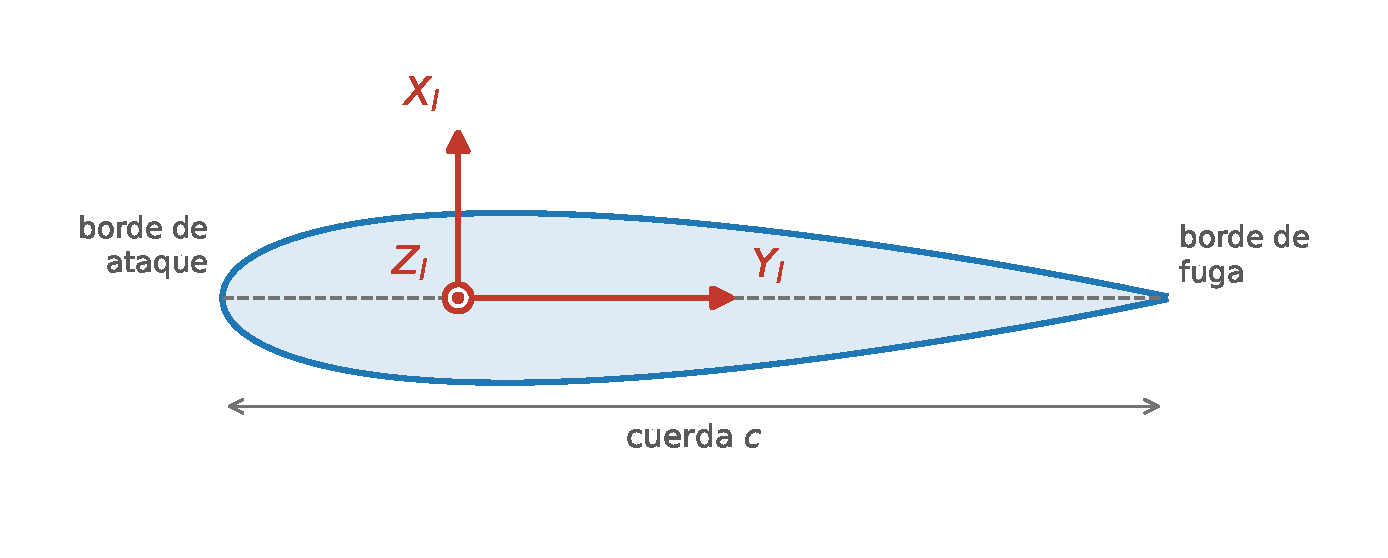
\includegraphics[width=0.75\textwidth]{Figuras/Figuras Metodología/ejes_locales_pala.pdf}
\caption[Sistema de ejes locales de la pala.]{Sistema de ejes locales de la pala sobre la sección del perfil: $X_l$ normal a la cuerda, $Y_l$ en el sentido de la cuerda hacia el borde de fuga y $Z_l$ a lo largo de la envergadura hacia la punta.}
\label{fig:ejes_locales}
\end{figure}

\subsubsection{Modelos aerodinámicos y pérdida dinámica}

Para la simulación en QBlade se selecciona el modelo de pérdida dinámica Gormont-Berg con constante de corrección $A_m = 6$, valor con el que \textcite{marten2019qblade} valida el modelo sobre un rotor Darrieus.

Los submodelos aerodinámicos complementarios que ofrece el software se configuran según su aplicabilidad a la geometría del rotor y a los grados de libertad del modelo. La aerodinámica no circulatoria, que incorpora el término de masa añadida asociado a la tasa de cabeceo por deformación torsional y a la deflexión de un flap~\parencite{marten2019qblade}, se mantiene desactivada, ya que el modelo no contempla flaps ni grado de libertad torsional. La corrección de sustentación y arrastre en dos puntos, se desactiva por corresponder a geometrías de diedro o cono, que las palas de un H-rotor de palas rectas no presenta~\parencite{QBladeDocsAero2024}. El efecto Himmelskamp, que describe el retraso de la pérdida producido por el adelgazamiento centrífugo de la capa límite y por la fuerza de Coriolis sobre una pala en rotación, y que QBlade implementa mediante la corrección de Snel~\parencite{marten2019qblade}, queda igualmente desactivado: dicha corrección escala con la razón entre la cuerda y la posición radial del elemento, magnitud que no varía en una pala que recorre su envergadura a radio constante. Se activa, en cambio, el modelo de sombra de torre, que superpone la solución de flujo potencial alrededor de un cilindro con un modelo de estela gobernado por el coeficiente de arrastre de la torre~\parencite{marten2019qblade}, ya que la pala describe su trayectoria en torno al eje central de la turbina y este perturba el flujo incidente. No se dispone del diámetro de ese eje, dato que fijaría el número de Reynolds del flujo a su alrededor y con él el valor preciso del coeficiente de arrastre. Ante esa indeterminación se adopta $C_{d,torre} = 1{,}0$, coherente con los valores que se manejan para secciones circulares en flujo transversal~\parencite{White2006}. Esta configuración se muestra en la Figura~\ref{fig:qblade_dynamic_stall}, tomada del módulo de definición de la turbina. Además de ser el valor utilizado por~\textcite{marten2019qblade}.

\begin{figure}[H]
\centering
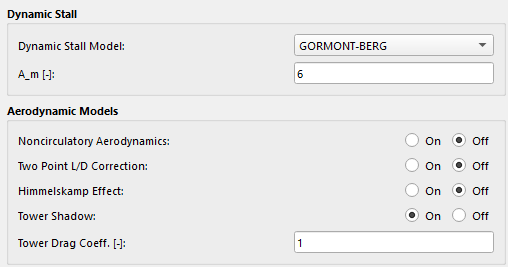
\includegraphics[width=0.6\textwidth]{Figuras/Figuras Metodología/qblade_dynamic_stall.png}
\caption{Modelo de pérdida dinámica Gormont-Berg y submodelos aerodinámicos configurados en el módulo de definición de la turbina de QBlade.}
\label{fig:qblade_dynamic_stall}
\end{figure}

\subsubsection{Modelo de estela LLFVW}

Para la resolución de la inducción del rotor se utiliza el método \gls{llfvw}. El esquema de integración de la convección de la estela se fija en Predictor-Corrector Backwards (PC2B), de segundo orden. Frente al esquema de primer orden de Euler, este duplica el número de evaluaciones del campo de velocidades por paso temporal, pero la mayor precisión que alcanza permite emplear un paso mayor manteniendo una exactitud aceptable~\parencite{marten2019qblade}, compensación pertinente en un conjunto de $102$ simulaciones de $600$~s.

Se habilita la auto-inducción de la estela (\textit{Wake Rollup}), sin la cual los filamentos no se deforman bajo su propio campo inducido y la estela deja de ser libre, condición que el método requiere para resolver la interacción de la pala con su propia estela. Se incluyen tanto los vórtices de arrastre (\textit{trailing}), que recogen la variación de la circulación ligada a lo largo de la envergadura, como los de desprendimiento (\textit{shed}), que recogen su variación en el tiempo. \textcite{marten2019qblade} señala que la circulación de estos últimos tiende a cero en simulaciones estacionarias con flujo incidente constante, caso en que su omisión acelera el cálculo sin pérdida apreciable. Esa condición no se cumple aquí, ya que el flujo incidente es turbulento y la circulación ligada varía además con el acimut a lo largo de cada revolución.

El transporte de los nodos de la estela (\textit{Wake Convection}) se configura en modo local, en el que la velocidad de convección se evalúa en la posición de cada nodo, en lugar de emplear la velocidad constante a la altura del centro del rotor o el perfil medio de la capa límite~\parencite{QBladeDocsAero2024}. Esta opción es la consistente con un campo de viento turbulento generado mediante el modelo de Mann, cuyas fluctuaciones varían en el espacio y en el tiempo.

La resolución del método LLFVW requiere definir los parámetros que controlan la discretización de la estela y el modelado de los vórtices, los cuales determinan la estabilidad numérica y la resolución espacial de la simulación. Estos parámetros se resumen en la Tabla~\ref{tab:parametros_estela}.

\begin{table}[H]
    \centering
    \caption{Parámetros de la estela y del modelado de vórtices configurados en QBlade.}
    \label{tab:parametros_estela}
    \begin{tabular}{lcc}
        \hline
        \textbf{Parámetro} & \textbf{Valor} & \textbf{Unidad} \\
        \hline
        \multicolumn{3}{c}{\textit{Malla de vórtices}} \\
        \hline
        Wake Relaxation Factor & $0{,}5$ & — \\
        Máximo de elementos de estela & $2 \times 10^5$ & — \\
        Distancia de truncamiento & $30$ & radios de rotor \\
        Wake Reduction Factor & $0{,}004$ & — \\
        Wake Zones (N/1/2/3) & $1$ / $4$ / $8$ / $12$ & revoluciones del rotor \\
        Refinamiento Streamwise (1/2/3) & $2$ / $2$ / $2$ & revoluciones del rotor \\
        Refinamiento Spanwise (1/2/3) & $1$ / $1$ / $2$ & revoluciones del rotor \\
        \hline
        \multicolumn{3}{c}{\textit{Modelado de vórtices}} \\
        \hline
        Bound Core Radius & $0{,}3$ & — \\
        Wake Core Radius & $0{,}1$ & — \\
        Turbulent Vortex Viscosity & $100$ & — \\
        Vortex Stretching & ON & — \\
        Max Vortex Stretching Factor & $50$ & — \\
        \hline
        \multicolumn{3}{c}{\textit{Iteración Gamma}} \\
        \hline
        Max Epsilon & $10^{-3}$ & — \\
        Max Number of Iterations & $100$ & — \\
        \hline
    \end{tabular}
\end{table}

Los valores adoptados provienen de la configuración con que \textcite{marten2019qblade} simula rotores Darrieus en QBlade, o se derivan de los criterios que esa misma fuente y la documentación del programa establecen. La longitud total de la estela, de $12$ revoluciones, es la que el autor reporta para su caso \gls{vawt} y la que, al \gls{tsr} de diseño, mantiene el error del coeficiente de potencia por debajo del $1\%$. Las zonas en que esa longitud se subdivide responden al método de engrosamiento progresivo de la estela, que reduce la resolución del reticulado por un factor entero cada vez que los filamentos alcanzan la edad que delimita cada zona; los factores en la dirección de la corriente reproducen el valor de $2$ del ejemplo documentado por el autor, mientras que en la dirección de la envergadura el engrosamiento se reserva para la última zona, la más alejada del rotor y la de menor influencia sobre la inducción. El factor de reducción adaptativa, de $0{,}004$, descarta los filamentos cuya circulación cae por debajo de esa fracción de la máxima presente en la estela~\parencite{QBladeDocsAero2024}, con lo que la misma fuente reporta una disminución del número de elementos a la mitad sin efecto apreciable sobre la exactitud; es además un valor más conservador que el que allí se emplea para \gls{vawt}, ya que descarta menos filamentos. El factor de relajación de la estela, de $0{,}5$, gobierna el desvanecimiento progresivo del vórtice de arranque, cuyo efecto sobre la solución se diluye así a medida que la estela se desarrolla~\parencite{QBladeDocsAero2024}. La distancia de truncamiento, expresada en radios de rotor, y el máximo de elementos operan como topes sobre el crecimiento del reticulado.

En el modelado de los vórtices, ambos radios de núcleo se definen como fracción de la cuerda local~\parencite{QBladeDocsAero2024}: el de la estela, de $0{,}1$, corresponde al $10\%$ que el autor propone como tamaño inicial del núcleo de los filamentos que se desprenden del borde de fuga, y el ligado, de $0{,}3$, fija el núcleo de los vórtices adheridos a la pala. La viscosidad turbulenta de $100$ es la que \textcite{marten2019qblade} reporta para su caso \gls{vawt}, y junto con los radios interviene en la ley con que el núcleo del vórtice crece a lo largo del tiempo. Activar el estiramiento de vórtices incorpora a esa misma ley la tasa de deformación del filamento, de modo que el núcleo responde al alargamiento que sufre al convectarse; el factor máximo de estiramiento, de $50$, es el umbral de deformación acumulada a partir del cual el filamento se retira de la estela~\parencite{QBladeDocsAero2024}.

La iteración Gamma, descrita en la Sección~\ref{sec:metodos_aerodinamicos}, resuelve la circulación ligada de los paneles en cada paso temporal. Sus dos parámetros acotan ese lazo: la circulación se actualiza hasta satisfacer el criterio de convergencia, fijado en $10^{-3}$, o hasta alcanzar el número máximo de iteraciones, fijado en $100$~\parencite{QBladeDocsAero2024}. El primero determina con qué exactitud queda resuelta la circulación antes de avanzar al paso siguiente; el segundo acota el costo y evita que un paso que no converja detenga la simulación.

Las Figuras~\ref{fig:qblade_wake_modeling} y~\ref{fig:qblade_vortex_modeling} muestran la configuración descrita en la interfaz de QBlade.

\begin{figure}[H]
\centering
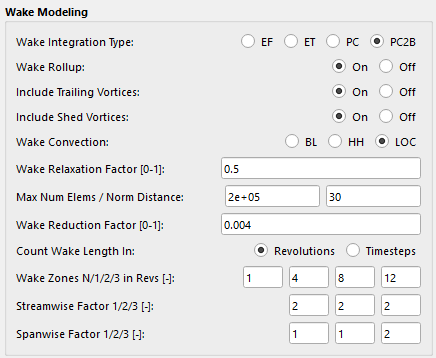
\includegraphics[width=0.5\textwidth]{Figuras/Figuras Metodología/qblade_wake_modeling.png}
\caption{Configuración de la estela, parámetros de truncamiento y refinamiento direccional en QBlade.}
\label{fig:qblade_wake_modeling}
\end{figure}

\begin{figure}[H]
\centering
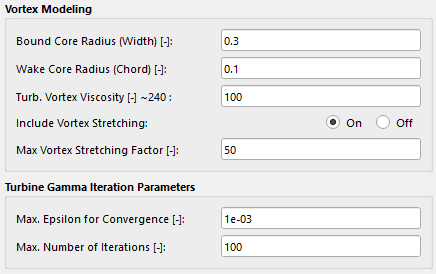
\includegraphics[width=0.5\textwidth]{Figuras/Figuras Metodología/qblade_vortex_modeling.png}
\caption{Modelado de vórtices y parámetros de convergencia de la iteración Gamma en QBlade.}
\label{fig:qblade_vortex_modeling}
\end{figure}

\subsubsection{Discretización temporal}
\label{sec:discretizacion_temporal}

La discretización temporal se especifica como un incremento acimutal y no como un paso de tiempo fijo. Se adopta $\Delta\theta = 5^\circ$, el incremento que \textcite{marten2019qblade} recomienda para la simulación aerodinámica y emplea en sus estudios sobre rotores Darrieus.

Definir el criterio sobre el ángulo y no sobre el tiempo lo independiza de la velocidad de rotación. El paso temporal queda determinado por $\Delta t = \Delta\theta / \Omega$, evaluado con la velocidad de rotación que la estrategia de control de la Sección~\ref{sec:control} asigna a cada velocidad de viento y mantenido fijo durante la simulación. Cada caso recibe así su propio paso, el mayor en $V_{in}$, donde la rotación es más lenta, y el menor una vez que esta alcanza su límite de diseño. Todos conservan los mismos $72$ pasos por revolución aunque $\Omega$ varíe con la velocidad del viento.

\subsubsection{Estrategia de control del rotor}
\label{sec:control}

Debido a que el campo de viento incorpora turbulencia, la velocidad incidente varía a lo largo de la simulación. Se implementa por ello el sistema de control descrito en la Sección~\ref{sec:control_teoria}, que mantiene el rotor en su \gls{tsr} óptimo, de modo que las simulaciones representen el funcionamiento normal de la turbina. Esta estrategia se adopta además por una razón de implementación, ya que es la que el programa admite integrar directamente en la simulación a través de su interfaz de controladores, sin requerir el desarrollo de una biblioteca de control propia~\parencite{QBladeDocsController2024}.

El rotor opera bajo dos regímenes, separados por la velocidad de viento a la que la rotación alcanza su valor máximo de diseño. Por debajo de esa velocidad se emplea el controlador $K$-$\omega^2$ de la Ec.~\ref{eq:K_omega2}, cuya constante se evalúa mediante la Ec.~\ref{eq:K_derivation} con los parámetros de diseño del rotor ($\rho = 1{,}225$~kg/m$^3$, $A = 476{,}79$~m$^2$, $R = 10{,}365$~m, $\lambda = 3{,}80$) y un coeficiente de potencia representativo $C_p = 0{,}45$. El valor resultante se presenta en el Capítulo~4.

Por sobre ella el controlador se desactiva y la velocidad de rotación se mantiene en ese valor máximo. Esta consigna se obtiene aplicando el criterio de la Sección~\ref{sec:criterio_rotacion}, que evalúa la Ec.~\ref{eq:omega_from_vtip} con el \gls{tsr} objetivo y la velocidad de viento nominal. El \gls{tsr} proviene del barrido DMST de la Sección~\ref{sec:dmst}, ejecutado como paso previo a las simulaciones de alta fidelidad precisamente para fijarla. La velocidad de viento nominal, que el fabricante no especifica, se adopta por analogía con las máquinas H-rotor de potencia y escala comparables, que alcanzan sus $200$~kW nominales a $12$~m/s (Tabla~\ref{tab:hrotor_rpm}). El desarrollo del cálculo, su contraste con el límite documentado para la T1-turbine y la solicitación centrífuga que la consigna implica se presentan en el Capítulo~4.

Los parámetros operacionales adoptados para las simulaciones se resumen en la Tabla~\ref{tab:parametros_operacionales}. A diferencia de los parámetros geométricos y de material (Tablas~\ref{tab:geometria_turbina} y~\ref{tab:material_pala}), estos no los proporciona el fabricante, sino que se definen por criterio de diseño a partir del análisis del recurso eólico y de la turbina de referencia.

Los dos límites del rango operacional se adoptan igualmente por criterio de diseño. La velocidad de arranque se fija en $V_{in} = 2$~m/s, y su plausibilidad se verifica a posteriori mediante las simulaciones \gls{llfvw}, que confirman la operación del rotor a esa velocidad (Capítulo~4). La velocidad de corte se fija en $V_{out} = 25$~m/s, valor que coincide con el documentado para la T1-turbine (Tabla~\ref{tab:t1_params}) y que responde al criterio de limitar las cargas extremas sobre la pala mediante la desconexión de la turbina, antes que a un óptimo de producción. La distribución de Weibull del emplazamiento no interviene en la elección de este valor, pero permite estimar lo que la desconexión cuesta: la frecuencia anual de vientos superiores a $25$~m/s, cuantificada en el Capítulo~4, resulta lo bastante baja como para que la producción sacrificada sea marginal. Las condiciones de viento extremo con la turbina detenida corresponden a los DLC 6.x, cuyo análisis queda fuera del alcance de este trabajo.

\begin{table}[H]
    \centering
    \caption{Parámetros operacionales adoptados y su procedencia.}
    \label{tab:parametros_operacionales}
    \begin{tabular}{lccl}
        \hline
        \textbf{Parámetro} & \textbf{Símbolo} & \textbf{Valor} & \textbf{Procedencia}\\
        \hline
        \gls{tsr} objetivo         & $\lambda$   & $3{,}80$    & DMST; corroborado por T1\\
        Velocidad máx.\ de rotación & $\Omega$    & Cap.~4      & criterio de la Sección~\ref{sec:criterio_rotacion}\\
        Velocidad de arranque      & $V_{in}$    & $2$ m/s     & Criterio de diseño (verificado LLFVW)\\
        Velocidad de corte         & $V_{out}$   & $25$ m/s    & Criterio de diseño (coincide con T1)\\
        Estrategia de control      & —           & $K$-$\omega^2$ & Criterio de diseño\\
        \hline
    \end{tabular}
\end{table}

\subsection{Selección de casos de carga según IEC 61400-1}

Los casos de carga de diseño (\acrshort{dlc}) se seleccionan conforme a la Sección 7 de la norma IEC 61400-1~\parencite{IEC61400-1}, adaptados a la configuración \gls{vawt} con base en el estudio de \textcite{Galinos2015}. El alcance del trabajo abarca la situación de producción de potencia, delimitación fundamentada en la Sección~\ref{sec:dlc_seleccion}. Dentro de esa situación la norma define cinco casos, de los cuales se adoptan los tres de naturaleza estocástica: DLC 1.1 (operación normal, NTM, ULS), DLC 1.2 (operación normal, NTM, fatiga) y DLC 1.3 (operación normal, ETM, ULS).

Los tres casos seleccionados cubren los dos estados límite que la norma exige verificar, el último y el de fatiga, y lo hacen sobre viento turbulento. Los dos restantes, DLC 1.4 y 1.5, quedan fuera por dos motivos. El primero es el tipo de fenómeno que representan. Ambos describen eventos transitorios que la norma define mediante perfiles determinísticos de ráfaga y de cizalladura, y no mediante un campo turbulento estocástico como el caracterizado para el emplazamiento. Analizarlos exige por ello una cadena de simulación y un tratamiento de resultados distintos de los desarrollados aquí, donde la carga de diseño se obtiene por vía estadística sobre múltiples semillas. El segundo motivo es el alcance del trabajo, circunscrito al funcionamiento nominal de la turbina, decisión que se apoya en la evidencia del Capítulo~2: es la operación normal con turbulencia la que origina las mayores cargas en la raíz de la pala. Con todo, este trabajo no demuestra que los casos excluidos no sean dimensionantes, aspecto que se retoma entre sus limitaciones.

Sobre los DLC seleccionados, la norma prescribe cuatro verificaciones estructurales para las palas:

\begin{itemize}
    \item \textbf{Resistencia última (ULS):} Comparación de los esfuerzos máximos con la resistencia última del material bajo los DLC 1.1 y 1.3.
    \item \textbf{Fatiga (FLS):} Estimación del daño acumulado durante la vida útil de diseño de $20$ años mediante el conteo de ciclos de carga del DLC 1.2.
    \item \textbf{Estabilidad (pandeo):} Verificación de que los paneles de la carcasa de la pala no experimenten inestabilidad global por pandeo bajo las combinaciones de carga más desfavorables.
    \item \textbf{Deflexión:} Verificación de que la deformación máxima de la pala no produzca interferencia mecánica con los brazos de soporte.
\end{itemize}

\subsection{Velocidades de simulación}
\label{sec:velocidades_simulacion}

Para los DLC 1.1 (ULS, NTM) y DLC 1.2 (fatiga, NTM), la Tabla 2 de la norma IEC 61400-1~\parencite{IEC61400-1} exige cubrir el rango completo de funcionamiento de la turbina, $V_{in} < V_{hub} < V_{out}$, y la norma fija en $2$~m/s la resolución con que ese rango se representa mediante un conjunto de valores discretos (Sección 7.4 de la norma IEC 61400-1)~\parencite{IEC61400-1}. Se seleccionan en consecuencia $12$ velocidades de viento en el centro del rotor, de $V = 2$ a $24$~m/s en intervalos de $\Delta V = 2$~m/s. Para el DLC 1.3 (ULS, ETM), la Tabla 2 de la misma norma prescribe considerar las velocidades que conducen a la condición más adversa para el diseño. Dado que las fuerzas aerodinámicas son proporcionales a $V^2$, esta condición se ubica en el extremo superior del rango operacional, seleccionándose $V = 16$, $18$, $20$, $22$ y $24$~m/s.

Todas las velocidades se simulan con $6$ realizaciones estocásticas de $600$~s cada una, que es el mínimo que la norma exige para cada velocidad de viento en el centro del rotor (Sección 7.5 de la norma IEC 61400-1)~\parencite{IEC61400-1}, totalizando $72$ simulaciones para los DLC 1.1/1.2 y $30$ simulaciones adicionales para el DLC 1.3. De cada realización se descartan los primeros $50$~s. Ese descarte lo impone la misma sección de la norma IEC 61400-1~\parencite{IEC61400-1}: puesto que las condiciones iniciales de una simulación dinámica afectan la estadística de cargas al comienzo del período simulado, la norma obliga a eliminar de todo intervalo de análisis con viento turbulento los primeros $5$~s de datos, o más si resulta necesario. Los $50$~s adoptados corresponden a esa ampliación: incluso en el caso más lento de la campaña, $V = 2$~m/s, donde la consigna $K$-$\omega^2$ de la Sección~\ref{sec:control} da $\Omega = \lambda V / R \approx 7{,}0$~rpm, ese tramo equivale a cerca de $6$ revoluciones completas del rotor; a las velocidades mayores, con $\Omega$ creciente, el número de revoluciones descartadas es aún mayor. Todas comparten además el incremento acimutal definido en la Sección~\ref{sec:discretizacion_temporal}, y se diferencian entre sí únicamente por la velocidad de referencia, por el modelo de turbulencia y por la semilla con que se genera el campo de viento. Las series temporales resultantes se procesan según los procedimientos de los Anexos F (DLC 1.1) y G (DLC 1.2) de la norma IEC 61400-1~\parencite{IEC61400-1}, y mediante el método de la media de máximos que la norma prescribe en su Sección 7.6.2 para el DLC 1.3~\parencite{IEC61400-1}. La Tabla~\ref{tab:matriz_simulaciones} detalla la matriz completa de simulaciones.

\begin{table}[H]
    \centering
    \caption{Matriz de simulaciones aerodinámicas por caso de carga y velocidad de viento ($\Delta\theta = 5^\circ$, $600$~s por realización).}
    \label{tab:matriz_simulaciones}
    \begin{tabular}{ccc}
        \hline
        \textbf{$V$ (m/s)} & \textbf{Realizaciones} & \textbf{Identificadores} \\
        \hline
        \multicolumn{3}{c}{\textit{DLC 1.1 y 1.2 (NTM): 72 simulaciones}} \\
        \hline
        $2$ & $6$ & 001--006 \\
        $4$ & $6$ & 007--012 \\
        $6$ & $6$ & 013--018 \\
        $8$ & $6$ & 019--024 \\
        $10$ & $6$ & 025--030 \\
        $12$ & $6$ & 031--036 \\
        $14$ & $6$ & 037--042 \\
        $16$ & $6$ & 043--048 \\
        $18$ & $6$ & 049--054 \\
        $20$ & $6$ & 055--060 \\
        $22$ & $6$ & 061--066 \\
        $24$ & $6$ & 067--072 \\
        \hline
        \multicolumn{3}{c}{\textit{DLC 1.3 (ETM): 30 simulaciones}} \\
        \hline
        $16$ & $6$ & 001--006 \\
        $18$ & $6$ & 007--012 \\
        $20$ & $6$ & 013--018 \\
        $22$ & $6$ & 019--024 \\
        $24$ & $6$ & 025--030 \\
        \hline
    \end{tabular}
\end{table}


\subsection{Factores parciales de seguridad}
\label{sec:factores_seguridad}

La verificación de la integridad estructural conforme a IEC 61400-1~\parencite{IEC61400-1} se fundamenta en el método de los estados límite, que emplea factores parciales de seguridad para cubrir las incertidumbres en las cargas, en las propiedades de los materiales y en las consecuencias de la falla. La norma distingue tres factores, que se justifican a continuación y cuyos valores para cada DLC se resumen al cierre de esta sección en la Tabla~\ref{tab:factores_seguridad}.

\subsubsection{Factor parcial de cargas ($\gamma_f$)}

El factor $\gamma_f$ cubre las desviaciones desfavorables de las cargas respecto de su valor característico y las incertidumbres del modelo de carga (Sección 7.6.1.1 de la norma IEC 61400-1)~\parencite{IEC61400-1}. Sus valores se prescriben en la Tabla 3 de la norma IEC 61400-1:

\begin{itemize}
    \item \textbf{DLC 1.1:} $\gamma_f = 1{,}25$. La norma reduce el factor general de $1{,}35$ a $1{,}25$ para el DLC 1.1 cuando las cargas se determinan mediante extrapolación estadística a 50 años según el Anexo F (Sección 7.6.2.1 de la norma IEC 61400-1, nota al pie de la Tabla 3)~\parencite{IEC61400-1}.
    \item \textbf{DLC 1.2 (fatiga):} $\gamma_f = 1{,}00$ para todas las situaciones normales y anormales (Sección 7.6.3.1 de la norma IEC 61400-1)~\parencite{IEC61400-1}, ya que en fatiga la incertidumbre se cubre por el lado de la resistencia del material.
    \item \textbf{DLC 1.3:} $\gamma_f = 1{,}35$, correspondiente a situaciones de diseño normales sin extrapolación estadística (Sección 7.6.2.1 de la norma IEC 61400-1, Tabla 3)~\parencite{IEC61400-1}.
\end{itemize}

Dado que el modelo de cálculo de cargas no ha sido validado mediante mediciones experimentales en una turbina similar, no aplica la reducción de $\gamma_f$ contemplada en la Sección 7.6.6 de la norma IEC 61400-1~\parencite{IEC61400-1} para modelos validados.

\subsubsection{Factor parcial de material ($\gamma_m$)}

El factor $\gamma_m$ cubre las desviaciones desfavorables de la resistencia del material, las incertidumbres geométricas y las diferencias entre las propiedades medidas en probetas y las reales en la estructura (Sección 7.6.1.1 de la norma IEC 61400-1)~\parencite{IEC61400-1}. La norma distingue según el tipo de verificación:

\begin{itemize}
    \item \textbf{ULS (resistencia última):} $\gamma_m = 1{,}30$. La Sección 7.6.2.2 de la norma IEC 61400-1~\parencite{IEC61400-1} prescribe $\gamma_m \geq 1{,}30$ para componentes estructurales no dúctiles (clase 2, no a prueba de fallos, \textit{non fail-safe}) cuya falla por tracción o compresión conduciría rápidamente a la falla de un componente principal de la turbina. El GFRP de la pala exhibe comportamiento lineal-elástico hasta rotura frágil~\parencite{Huh2012,Moraras2023}, lo que lo clasifica como material no dúctil.
    \item \textbf{Fatiga:} $\gamma_m = 1{,}70$. La Sección 7.6.3.2 de la norma IEC 61400-1~\parencite{IEC61400-1} prescribe $\gamma_m \geq 1{,}70$ para materiales compuestos con coeficiente de variación de la resistencia a fatiga entre el $15\%$ y el $20\%$, cuando la curva S-N se basa en una probabilidad de supervivencia del $50\%$~\parencite{Huh2012}. Este valor es conservador; la norma permite reducirlo a $1{,}20$ si la curva S-N se deriva con un $95\%$ de supervivencia y $95\%$ de confianza.
\end{itemize}

\subsubsection{Factor parcial de consecuencia de falla ($\gamma_n$)}

El factor $\gamma_n$ distingue entre clases de componentes según la criticidad de su falla, conforme a la Sección 7.6.1.2 de la norma IEC 61400-1~\parencite{IEC61400-1}. La pala del aerogenerador se clasifica como componente clase 2 (no a prueba de fallos, \textit{non fail-safe}), cuya falla puede conducir a la falla de una parte principal de la turbina. En verificaciones de resistencia última, la norma establece $\gamma_n = 1{,}00$ (Sección 7.6.2.2 de la norma IEC 61400-1)~\parencite{IEC61400-1}. Para fatiga, el factor se incrementa a $\gamma_n = 1{,}15$ (Sección 7.6.3.2 de la norma IEC 61400-1)~\parencite{IEC61400-1}, reflejando la mayor incertidumbre asociada a la acumulación de daño cíclico en materiales compuestos.

\subsubsection{Verificación de resistencia última}

La condición de estado límite último se expresa mediante la ecuación (31) de la norma IEC 61400-1~\parencite{IEC61400-1}, reproducida en la Ec.~\ref{eq:uls_verification}:

\begin{equation}
    \gamma_n \cdot \gamma_f \cdot F_k \leq \frac{f_k}{\gamma_m}
    \label{eq:uls_verification}
\end{equation}

donde $F_k$ es la carga característica, $f_k$ es la resistencia característica del material, y los factores $\gamma_f$, $\gamma_m$ y $\gamma_n$ toman los valores indicados en la Tabla~\ref{tab:factores_seguridad} según el DLC correspondiente. Las cargas de diseño $F_d = \gamma_f \cdot F_k$ incorporan el factor de carga y constituyen la entrada directa al modelo de elementos finitos (Sección~\ref{sec:fem}). La verificación en tensión se reduce a la Ec.~\ref{eq:uls_stress}:

\begin{equation}
    \sigma_{\max} \leq \frac{\sigma_u}{\gamma_m \cdot \gamma_n}
    \label{eq:uls_stress}
\end{equation}

donde $\sigma_{\max}$ es la mayor tensión principal que entrega el modelo de elementos finitos bajo las cargas de diseño y $\sigma_u$ la resistencia última del material (Tabla~\ref{tab:material_pala}).

Para el DLC 1.1 y DLC 1.3, la resistencia factoreada se obtiene como $\sigma_u / (\gamma_m \cdot \gamma_n)$, con $\gamma_m = 1{,}30$ y $\gamma_n = 1{,}00$ según la Tabla~\ref{tab:factores_seguridad}. Los valores numéricos se presentan en el Capítulo~4.

\subsubsection{Verificación de fatiga}

En la verificación de fatiga, todos los factores parciales ($\gamma_f = 1{,}00$, $\gamma_m = 1{,}70$, $\gamma_n = 1{,}15$) se aplican al rango de tensión cíclica, según lo prescrito en la Sección 7.6.3 de la norma IEC 61400-1~\parencite{IEC61400-1}. La curva S-N resultante (Ec.~\ref{eq:basquin_design}) y el procedimiento completo de cálculo de daño se detallan en la Sección~\ref{sec:anexo_g} (DLC 1.2).

La Tabla~\ref{tab:factores_seguridad} reúne los valores que resultan de los tres apartados anteriores y que se aplican en cada uno de los DLC considerados.

\begin{table}[H]
    \centering
    \caption{Factores parciales de seguridad aplicados según DLC y tipo de verificación.}
    \label{tab:factores_seguridad}
    \begin{tabular}{lcccc}
        \hline
        \textbf{Factor} & \textbf{Símbolo} & \textbf{DLC 1.1 (ULS)} & \textbf{DLC 1.2 (Fatiga)} & \textbf{DLC 1.3 (ULS)} \\
        \hline
        Cargas & $\gamma_f$ & $1{,}25$ & $1{,}00$ & $1{,}35$ \\
        Material & $\gamma_m$ & $1{,}30$ & $1{,}70$ & $1{,}30$ \\
        Consecuencia de falla & $\gamma_n$ & $1{,}00$ & $1{,}15$ & $1{,}00$ \\
        \hline
    \end{tabular}
\end{table}

\subsection{Procesamiento de cargas aerodinámicas}
\label{sec:procesamiento_cargas}

Cada uno de los tres DLC seleccionados responde a una pregunta de verificación distinta y, por ello, recibe un tratamiento estadístico propio:

\begin{itemize}
    \item \textbf{DLC 1.1} responde a cuál es la carga extrema que la pala debe resistir a lo largo de su vida. Como las simulaciones abarcan minutos y la vida de diseño abarca décadas, el máximo observado no basta: la norma exige extrapolar estadísticamente los máximos a un período de retorno de 50 años mediante el procedimiento de su Anexo F~\parencite{IEC61400-1}.
    \item \textbf{DLC 1.2} responde a si la pala sobrevive la acumulación de daño por fatiga durante los 20 años de vida de diseño. Aquí no interesa el máximo sino el espectro completo de ciclos de carga, que se obtiene por conteo Rainflow conforme al Anexo G de la norma IEC 61400-1~\parencite{IEC61400-1} y se acumula mediante la regla de Palmgren-Miner~\parencite{Miner1945}, ponderando cada velocidad de viento por su permanencia anual según la distribución de Weibull del emplazamiento.
    \item \textbf{DLC 1.3} responde a cuál es la carga extrema bajo una turbulencia excepcionalmente intensa. A diferencia del DLC 1.1, la severidad no proviene de extrapolar en el tiempo sino de un modelo de turbulencia más severo (ETM), por lo que la norma no requiere extrapolación: la carga característica es la media de los máximos de las realizaciones.
\end{itemize}

A continuación se describe el procesamiento aplicado a las series temporales de fuerzas obtenidas de las simulaciones en QBlade para cada uno de estos tres casos. Los factores parciales de seguridad $\gamma_f$, $\gamma_m$ y $\gamma_n$ empleados en cada caso corresponden a los valores definidos en la Tabla~\ref{tab:factores_seguridad}.

\subsubsection{DLC 1.1 --- estado límite último}
\label{sec:anexo_f}

El procedimiento de extrapolación estadística del Anexo F, informativo, de la IEC 61400-1~\parencite{IEC61400-1} determina la carga característica a 50 años a partir de los máximos observados en simulaciones de corta duración. La norma exige aplicar el Anexo F sobre una única señal escalar (Sección 7.5 de la norma IEC 61400-1)~\parencite{IEC61400-1}: en este trabajo dicha señal se construye como la fuerza total integrada sobre la pala, $F_{tot}(t)$. Todo el procedimiento que sigue proviene de ese anexo, por lo que sus secciones se citan de forma reiterada a lo largo de los pasos que se detallan a continuación.

\medskip
\noindent\textbf{Señal escalar de carga.}
Cada una de las 72 simulaciones produce, en cada paso temporal, 24 pares de fuerzas aerodinámicas por unidad de longitud $(F_{x,l,i}, F_{y,l,i})$ distribuidas a lo largo de la envergadura de la pala. El subíndice $l$ indica que las componentes se expresan en el sistema local de la pala (Figura~\ref{fig:ejes_locales}) y el subíndice $i$ identifica la estación de medición. Los subíndices $x$ e $y$ corresponden a las dos direcciones de ese sistema contenidas en el plano del perfil: $x$ es normal a la cuerda e $y$ corre a lo largo de ella hacia el borde de fuga. Ambas componentes se reúnen en una sola señal $F_{tot}(t)$ mediante el módulo del vector que forman en cada estación, ponderado por la longitud de pala que esa estación representa, según la Ec.~\ref{eq:F_tot}:

\begin{equation}
    F_{tot}(t) = \sum_{i=1}^{24} \sqrt{F_{x,l,i}^2(t) + F_{y,l,i}^2(t)} \cdot \Delta s_i
    \label{eq:F_tot}
\end{equation}

donde $\Delta s_i$ es la longitud de pala que concentra la estación $i$, y el producto convierte la fuerza por unidad de longitud que entrega cada sensor en la fuerza, en newton, del tramo que le corresponde. Las 24 estaciones se reparten uniformemente sobre los $23$~m de envergadura, como se ve en la Figura~\ref{fig:delta_s}.

\begin{figure}[H]
\centering
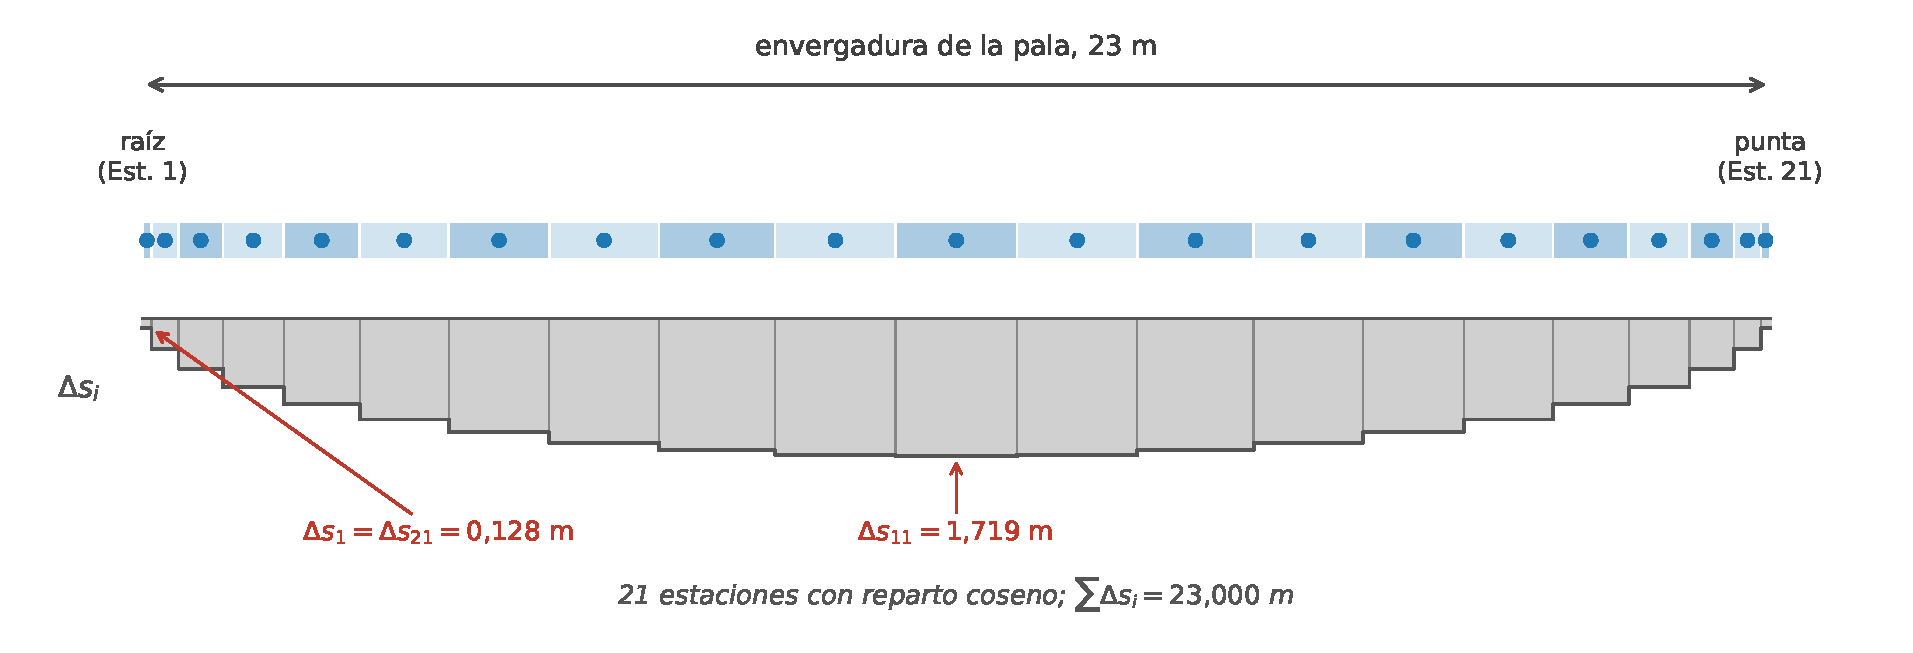
\includegraphics[width=0.95\textwidth]{Figuras/Figuras Metodología/estaciones_delta_s.pdf}
\caption[Tramo de pala que representa cada estación.]{Tramo de pala $\Delta s_i$ que representa cada una de las 24 estaciones.}
\label{fig:delta_s}
\end{figure}
 La raíz reúne las dos componentes en el módulo de la fuerza que actúa sobre cada estación, magnitud siempre positiva, de modo que la suma a lo largo de la envergadura no admite cancelaciones entre estaciones con carga de sentido opuesto y recoge la solicitación completa que soporta la pala.

\medskip
\noindent\textbf{Máximos por simulación y ajuste de Gumbel.}
Para cada velocidad de viento $V_j$ se dispone de $6$ simulaciones, una por semilla estocástica del campo de viento turbulento (Sección~\ref{sec:campo_turbulento}), de modo que las seis representan realizaciones independientes de un mismo proceso estocástico. De cada una se extrae el mayor valor que alcanza $F_{tot}(t)$ sobre el intervalo $t \geq 50$~s (Sección~\ref{sec:velocidades_simulacion}). Ese valor se denota $F_{max}$ y es la variable sobre la que opera todo el procedimiento que sigue: cada realización aporta una observación, de modo que a la velocidad $V_j$ se cuenta con seis. Extraer un único máximo por realización es coherente con la definición normativa de la carga característica, referida al mayor valor que se presenta en un intervalo de diez minutos (Sección 7.6.2 de la norma IEC 61400-1)~\parencite{IEC61400-1}.

Sobre esas seis observaciones se ajusta la distribución de Gumbel presentada en la Sección~\ref{sec:extrapolacion_teoria}, cuya función de distribución acumulada es la Ec.~\ref{eq:gumbel_anexof}, evaluada aquí en $F = F_{max}$. Sus dos parámetros, el de posición $\mu_j$ y el de escala $\beta_j$, se estiman por el método de los momentos, que iguala la media y la varianza de la distribución a las de la muestra. Para la distribución de Gumbel la media vale $\mu_j + \gamma_E \beta_j$ y la varianza $\pi^2 \beta_j^2 / 6$~\parencite{Gumbel1958}, de donde se despejan los estimadores de las Ecs.~\ref{eq:gumbel_beta} y~\ref{eq:gumbel_mu}:

\begin{equation}
    \beta_j = \frac{\sqrt{6}}{\pi}\,\sigma_{max,j}
    \label{eq:gumbel_beta}
\end{equation}

\begin{equation}
    \mu_j = \overline{F}_{max,j} - \gamma_E\,\beta_j
    \label{eq:gumbel_mu}
\end{equation}

donde $\overline{F}_{max,j}$ y $\sigma_{max,j}$ son la media y la desviación estándar de las seis observaciones de $F_{max}$ a la velocidad $V_j$, y $\gamma_E = 0{,}5772$ es la constante de Euler-Mascheroni~\parencite{Havil2003}. El subíndice $j$ recorre las doce velocidades simuladas, de manera que el ajuste entrega un par $(\mu_j, \beta_j)$ por cada una.

\medskip
\noindent\textbf{Probabilidad de excedencia condicionada a la velocidad.}
La Gumbel ajustada en el paso anterior permite calcular, para una velocidad fija $V_j$, la probabilidad de que $F_{max}$ supere un nivel de carga dado. En lo que sigue ese nivel se designa también $F_{max}$, por tratarse de la misma variable recién definida. La probabilidad condicional es el complemento de la función de distribución, según la Ec.~\ref{eq:pe_cond}:

\begin{equation}
    P_e(F_{max} \mid V_j) = 1 - \Phi(F_{max}; \mu_j, \beta_j)
    \label{eq:pe_cond}
\end{equation}

\medskip
\noindent\textbf{Integración de largo plazo con la distribución de Weibull.}
La probabilidad anterior está condicionada a una velocidad fija. Dado que cada velocidad $V_j$ ocurre con una frecuencia distinta a lo largo del año, se requiere la probabilidad de excedencia no condicionada. Para obtenerla, la norma prescribe integrar sobre la distribución de velocidades de viento en el emplazamiento (Ecuación F.2 del Anexo F de la norma IEC 61400-1)~\parencite{IEC61400-1}. Esa distribución es la densidad de Weibull de la Ec.~\ref{eq:weibull_pdf_general}, con los parámetros $k$ y $c$ ajustados a la altura del centro del rotor ($z = 21{,}3$~m) según el procedimiento de la Sección~\ref{sec:recurso_metodo}, cuyos valores se reportan en el Capítulo~4.

Numéricamente, la integral se discretiza en $N_V = 25$ intervalos de ancho $\Delta V = 1$~m/s, centrados en $V = 0{,}5; 1{,}5; \dots; 24{,}5$~m/s. Como solo se dispone de datos de Gumbel en las $12$ velocidades de simulación, los parámetros $\mu(V)$ y $\beta(V)$ se interpolan linealmente para los $25$ intervalos. La probabilidad de excedencia de largo plazo resulta según la Ec.~\ref{eq:pe_longterm}:

\begin{equation}
    P_e(F_{max}) = \sum_{m=1}^{N_V} \Bigl[1 - \exp\!\bigl(-e^{-(F_{max} - \mu(V_m))/\beta(V_m)}\bigr)\Bigr] \cdot f_W(V_m) \cdot \Delta V
    \label{eq:pe_longterm}
\end{equation}

En esta expresión, cada velocidad se pondera por su frecuencia de ocurrencia anual según la distribución de Weibull: las velocidades cercanas a $V_{ave}$ reciben mayor peso a pesar de producir fuerzas moderadas, mientras que las velocidades próximas a $V_{out}$ reciben menor peso aunque generan fuerzas mayores. La combinación de ambos efectos, frecuencia Weibull y magnitud Gumbel, determina la contribución relativa de cada velocidad al riesgo de excedencia a largo plazo.

\medskip
\noindent\textbf{Bisección para la carga característica a 50 años.}
La norma define la carga característica $F_k$ como aquella cuya probabilidad de ser superada en el período de retorno de diseño es exactamente $T_{obs} / T_{retorno}$, según la Ec.~\ref{eq:fk_criterion}:

\begin{equation}
    P_e(F_k) = \frac{T_{\text{obs}}}{T_{\text{retorno}}}
    \label{eq:fk_criterion}
\end{equation}

con $T_{obs} = 600$~s el período de observación de cada realización y $T_{retorno} = 50$ años el de diseño; el valor numérico de esta probabilidad objetivo se presenta en el Capítulo~4. La raíz $F_k$ se determina numéricamente por bisección sobre la Ec.~\ref{eq:pe_longterm}: se prueban valores de $F_{max}$, se evalúa $P_e(F_{max})$, y se ajusta el intervalo de búsqueda hasta alcanzar la probabilidad objetivo. La carga característica $F_k$ es el valor de $F_{max}$ que la satisface.

\medskip
\noindent\textbf{Carga de diseño.}
La carga característica $F_k$ es un valor estadístico; la carga de diseño $F_d$ incorpora además un margen para cubrir las incertidumbres del modelo de carga y de la extrapolación estadística. Se obtiene mayorando la carga característica por el factor parcial de carga, según la Ec.~\ref{eq:fd_anexof} de la Sección~\ref{sec:extrapolacion_teoria} (Ecuación 28, Sección 7.6.1.1 de la norma IEC 61400-1)~\parencite{IEC61400-1}, con $\gamma_f = 1{,}25$; ver su justificación en la Sección~\ref{sec:factores_seguridad}.

\medskip
\noindent\textbf{Perfil espacial de fuerzas de diseño.}
El Anexo F de la IEC 61400-1~\parencite{IEC61400-1} proporciona un único valor escalar $F_d$, que debe distribuirse a lo largo de la envergadura para cargar el modelo de elementos finitos. Esa distribución se resuelve en las mismas 24 estaciones con que se decidió instrumentar la pala (Sección~\ref{sec:discretizacion}), obteniéndose un vector de 24 fuerzas de diseño $(F_{d,x}[p], F_{d,y}[p])$, una por estación. Para preservar la correlación espacial entre estaciones, el perfil de carga se extrae del instante de máxima solicitación global en la realización que registró la mayor solicitación (Sección 7.5 de la norma IEC 61400-1)~\parencite{IEC61400-1}: se capturan las fuerzas compañeras $F_x[p], F_y[p]$ en ese $t_{max}$ y se escalan uniformemente por el factor $F_d / F_{tot}(t_{max})$. Este enfoque garantiza que la distribución espacial de fuerzas que ingresa al FEM sea la que entrega la simulación aerodinámica en ese único instante, con la correlación entre estaciones que ella misma produce, y no una combinación artificial de máximos independientes por estación que no ocurrieron simultáneamente; y que la magnitud global sea consistente con la carga de diseño a 50 años, ya que todas las estaciones provienen del mismo instante de la simulación. Las fuerzas se transfieren al modelo estructural conservando su signo, de modo que la dirección de aplicación reproduce la del instante gobernante. La Tabla~\ref{tab:anexo_fuerzas_dlc11} del \hyperref[anexo:fuerzas]{Anexo~A} presenta, para las 24 estaciones, tanto la fuerza $F_{sim,x}[p], F_{sim,y}[p]$ que entrega la simulación en el instante $t_{max}$ como la fuerza puntual de diseño $F_{d,x}[p], F_{d,y}[p]$ que resulta de escalarla y de aplicarla como carga remota en el modelo FEM; las direcciones $x$ e $y$ corresponden a los ejes locales de la Figura~\ref{fig:ejes_locales}.

\bigskip
\subsubsection{DLC 1.2 --- fatiga}
\label{sec:anexo_g}

Las mismas 72 series temporales empleadas para el DLC 1.1 se procesan conforme al Anexo G, informativo, de la IEC 61400-1~\parencite{IEC61400-1} para estimar el daño acumulado por fatiga durante la vida útil de diseño de $20$ años, valor que corresponde al mínimo exigido por la norma para las turbinas de clase I a III (Sección 6.2 de la norma IEC 61400-1)~\parencite{IEC61400-1}.

\medskip
\noindent\textbf{Variable de carga: momento flector en la sección crítica.}
En la configuración VAWT analizada, la pala se une al eje mediante dos brazos o \textit{struts} (Tabla~\ref{tab:geometria_turbina}), de modo que estructuralmente se comporta como una viga apoyada en esos dos puntos, con un tramo en voladizo en cada extremo. En cada instante de la simulación aerodinámica, las fuerzas distribuidas a lo largo de la envergadura flectan la pala y producen en cada sección transversal un momento flector, cuya magnitud depende de las fuerzas que actúan sobre el tramo que esa sección sostiene y de la distancia a la que lo hacen. El procedimiento de fatiga consiste, en términos simples, en calcular a partir de esas fuerzas el momento flector que soporta la sección más solicitada en cada instante, traducirlo a tensión mediante un factor de proporcionalidad calibrado con una única corrida del modelo de elementos finitos, y contar sobre la serie temporal de tensión así obtenida los ciclos que acumulan daño.

Se denomina sección crítica a la sección transversal de la pala en que la simulación FEM bajo carga estática (Sección~\ref{sec:fem}) registra la mayor tensión principal, y $z_{crit}$ a su coordenada sobre la envergadura, medida desde la base de la pala ($z = 0$) hasta esa sección. Su ubicación se desprende del análisis FEM y se reporta en el Capítulo~4.

El tramo que solicita a esa sección es el voladizo que ella sostiene, esto es, el conjunto de estaciones comprendidas entre el extremo libre de la pala y la sección crítica. Cuando la sección crítica corresponde a la conexión con el brazo inferior, ese tramo lo forman las estaciones situadas bajo ella, y las componentes del momento flector se obtienen según las Ecs.~\ref{eq:Mx_fatiga} y~\ref{eq:My_fatiga}:

\begin{align}
    M_x(t) &= \sum_{i:\, z_i < z_{crit}} F_{y,i}(t) \cdot (z_{crit} - z_i)
    \label{eq:Mx_fatiga} \\[4pt]
    M_y(t) &= \sum_{i:\, z_i < z_{crit}} F_{x,i}(t) \cdot (z_{crit} - z_i)
    \label{eq:My_fatiga} \\[4pt]
    M_{res}(t) &= \sqrt{M_x^2(t) + M_y^2(t)}
    \label{eq:Mres_fatiga}
\end{align}

donde el subíndice $i$ recorre las $24$ estaciones en que se discretizó la pala (Sección~\ref{sec:discretizacion}); $z_i$ es la coordenada de la estación $i$ sobre la envergadura (m) y $(z_{crit} - z_i)$, el brazo de palanca con que su carga actúa sobre la sección crítica; $F_{x,i}$ y $F_{y,i}$ son las fuerzas puntuales que aporta la estación $i$ en cada instante (N), obtenidas al multiplicar la fuerza por unidad de longitud que entrega la simulación por la longitud de pala $\Delta s_i$ que la estación representa, en las dos direcciones del sistema local de la Figura~\ref{fig:ejes_locales}. Las componentes $M_x$ y $M_y$ son los momentos flectores que actúan sobre la sección crítica en torno a cada uno de los dos ejes locales del perfil: $M_x$ flecta la pala en torno al eje $X_l$ y lo genera la componente de fuerza $F_y$, mientras que $M_y$ flecta en torno al eje $Y_l$ y lo genera $F_x$. El momento flector resultante $M_{res}$ es el módulo del vector que ambas componentes forman y constituye la variable de carga del análisis de fatiga. A diferencia de la fuerza total integrada $F_{tot}(t)$ empleada en el DLC 1.1, $M_{res}(t)$ se vincula directamente al mecanismo de falla por fatiga, ya que la tensión en la sección crítica es proporcional al momento resultante.

\medskip
\noindent\textbf{Conversión momento--tensión.}
Bajo la hipótesis de linealidad elástica del GFRP hasta rotura~\parencite{Huh2012,Moraras2023}, la tensión en el punto crítico admite descomponerse en dos contribuciones de naturaleza distinta. La aerodinámica fluctúa con el viento y es proporcional al momento flector resultante; la inercial, producida por la aceleración centrífuga y la gravedad, es constante mientras el rotor gira a su velocidad de consigna y no depende del momento aerodinámico. La historia de tensión en la sección crítica se construye en consecuencia según la Ec.~\ref{eq:sigma_from_M}:

\begin{equation}
    \sigma(t) = K_{aero} \cdot M_{res}(t) + \sigma_{in}
    \label{eq:sigma_from_M}
\end{equation}

donde $\sigma_{in}$ es la tensión principal máxima que el modelo FEM registra en la sección crítica bajo las cargas inerciales como única solicitación, y $K_{aero}$ el factor que traduce momento aerodinámico en tensión. Este último se obtiene de las mismas dos corridas del modelo FEM, según la Ec.~\ref{eq:keff}:

\begin{equation}
    K_{aero} = \frac{\sigma_{1,\max} - \sigma_{in}}{M_{res,d}}
    \label{eq:keff}
\end{equation}

donde $\sigma_{1,\max}$ es la tensión principal máxima bajo la carga de diseño completa del DLC 1.1, que incluye las cargas inerciales, y $M_{res,d}$ el momento flector resultante que producen las fuerzas aerodinámicas de diseño, evaluado mediante la Ec.~\ref{eq:Mres_fatiga}. Restar $\sigma_{in}$ del numerador aísla la fracción de tensión que efectivamente escala con el momento: calibrar el factor sobre la tensión total atribuiría al momento aerodinámico una contribución inercial que no depende de él, y sobreestimaría por ello la amplitud de todos los ciclos. Este enfoque es consistente con la formulación del Anexo G (Sección G.1 de la norma IEC 61400-1)~\parencite{IEC61400-1}, que permite asumir que la tensión local en el punto de falla es linealmente proporcional a la carga.

\medskip
\noindent\textbf{Conteo de ciclos Rainflow.}
Cada una de las 72 series temporales de tensión $\sigma(t)$, con una duración efectiva de $T_{sim} = 550$~s, se procesa mediante el algoritmo de conteo de ciclos Rainflow (Anexo G, Sección G.1 de la norma IEC 61400-1)~\parencite{IEC61400-1}, cuyo fundamento se expone en la Sección~\ref{sec:anexo_g_antecedentes}. La implementación empleada sigue la formulación de cuatro puntos normalizada en la práctica ASTM E1049-85~\parencite{ASTM_E1049}, correspondiente al método propuesto originalmente por \textcite{Matsuishi1968}. El algoritmo descompone la señal en ciclos individuales caracterizados por su amplitud $\sigma_a$ y su tensión media $\sigma_m$, preservando la secuencia de carga tal como ocurre en la simulación.

\medskip
\noindent\textbf{Corrección por tensión media.}
Cada ciclo se refiere a media nula mediante el diagrama de vida constante descrito en la Sección~\ref{sec:anexo_g_antecedentes}, con la tensión media $\sigma_m$ que entrega el propio conteo Rainflow y que incorpora, por construcción de la Ec.~\ref{eq:sigma_from_M}, la contribución inercial $\sigma_{in}$. Se adopta la formulación lineal de Goodman (Ec.~\ref{eq:goodman}) antes que la de Gerber porque \textcite{Huh2012}, la misma fuente de la que provienen la curva S-N y el exponente de fatiga empleados, contrasta ambas sobre este material y reporta que la de Goodman subestima la vida a fatiga del tejido bidireccional para tensiones medias superiores a $40$~MPa, esto es, resulta la conservadora de las dos en el rango que aquí interesa.

\medskip
\noindent\textbf{Curva S-N del material.}
La resistencia a fatiga del GFRP se modela mediante la ecuación de Basquin en su forma factorizada~\parencite{Basquin1910}. La norma prescribe que todos los factores parciales de seguridad se apliquen al rango de tensión cíclica (Sección 7.6.3 de la norma IEC 61400-1)~\parencite{IEC61400-1}, según la Ec.~\ref{eq:sigma_eq}:

\begin{equation}
    \sigma_{a,\text{eq}} = \gamma_f \cdot \gamma_m \cdot \gamma_n \cdot \sigma_{a,0}
    \label{eq:sigma_eq}
\end{equation}

donde $\sigma_{a,0}$ es la amplitud corregida por tensión media de la Ec.~\ref{eq:goodman}, y $\sigma_{a,\text{eq}}$ la amplitud de tensión equivalente de diseño, mayorada por los tres factores parciales de fatiga justificados en la Sección~\ref{sec:factores_seguridad}: $\gamma_f$ (carga), $\gamma_m$ (material) y $\gamma_n$ (consecuencia de falla).

La curva S-N de diseño, que relaciona la amplitud de tensión equivalente con el número de ciclos admisible, se expresa según la Ec.~\ref{eq:basquin_design}:

\begin{equation}
    \sigma_{a,\text{eq}} = \sigma_u \cdot (2N_f)^b
    \label{eq:basquin_design}
\end{equation}

Sustituyendo las Ecs.~\ref{eq:goodman} y~\ref{eq:sigma_eq} en la Ec.~\ref{eq:basquin_design} y despejando $N_f$ se obtiene la expresión utilizada en el cálculo de daño:

\begin{equation}
    N_{f} = \frac{1}{2}\left(\frac{\gamma_f \cdot \gamma_m \cdot \gamma_n}{\sigma_u} \cdot \frac{\sigma_{a}}{1 - \sigma_m / \sigma_u}\right)^{1/b}
    \label{eq:Nf_fatiga}
\end{equation}

donde $\sigma_u = 242{,}1$~MPa (resistencia última entregada por el fabricante de la pala, Tabla~\ref{tab:material_pala}), $b = -0{,}045$ (exponente de fatiga para tejido bidireccional $\pm 45^\circ$ fabricado por infusión al vacío~\parencite{Huh2012}) y $\gamma_f$, $\gamma_m$, $\gamma_n$ los factores parciales de fatiga justificados en la Sección~\ref{sec:factores_seguridad}.

\medskip
\noindent\textbf{Construcción del espectro colectivo anual.}
Cada simulación de $T_{sim} = 550$~s corresponde a una velocidad de viento fija $V_j$ y produce, mediante Rainflow, un conjunto de ciclos de fatiga $(\sigma_a, \sigma_m)$. Estos ciclos representan la operación continua del aerogenerador durante $550$~s a dicha velocidad. Para construir el espectro representativo de un año completo, los ciclos de cada velocidad se expanden proporcionalmente a la fracción de tiempo que el viento permanece en ese intervalo en el emplazamiento.

La fracción de tiempo anual asociada a la velocidad $V_j$ se obtiene de la distribución de Weibull que caracteriza el sitio (Ec.~\ref{eq:weibull_pdf_general}), según la Ec.~\ref{eq:tiempo_anual}:

\begin{equation}
    t_j = f_W(V_j) \cdot \Delta V \cdot 365{,}25 \cdot 24 \cdot 3600 \quad [\text{s/año}]
    \label{eq:tiempo_anual}
\end{equation}

donde $f_W(V_j)$ es la densidad de probabilidad Weibull evaluada en $V_j$, $\Delta V = 2$~m/s es el ancho del intervalo de velocidad, y $365{,}25 \cdot 24 \cdot 3600$ es la duración de un año calendario en segundos, considerando el promedio de $365{,}25$ días que incorpora los años bisiestos; no es un valor prescrito por la norma, sino la conversión que lleva la densidad de probabilidad a una tasa temporal. La Tabla~\ref{tab:weibull_fatiga} en el Capítulo~4 presenta, para las doce velocidades $V_j$ del rango operacional, los valores de $f_W(V_j)$, $t_j$ y el factor de escalamiento temporal $t_j / T_{sim}$.

El número de ciclos anuales atribuibles a la velocidad $V_j$ se calcula escalando los ciclos simulados (Ecuación G.7 del Anexo G de la norma IEC 61400-1)~\parencite{IEC61400-1}, según la Ec.~\ref{eq:espectro_anual}:

\begin{equation}
    n_{j}^{\text{anual}} = \bar{n}_{j}^{\text{sim}} \cdot \frac{t_j}{T_{sim}}
    \label{eq:espectro_anual}
\end{equation}

donde $\bar{n}_{j}^{\text{sim}}$ es el número promedio de ciclos de las $6$ semillas a la velocidad $V_j$, es decir, de las seis series generadas con una semilla estocástica distinta, el entero que inicializa el generador de números aleatorios del campo de turbulencia y que hace que cada serie sea una realización independiente del mismo proceso estocástico (Sección~\ref{sec:campo_turbulento}). Las $72$ series simuladas ($12$ velocidades $\times$ $6$ semillas) se agrupan por velocidad de viento y los ciclos de las $6$ semillas se promedian antes del escalamiento temporal para reducir la variabilidad estocástica. El espectro colectivo anual se construye sumando las contribuciones de las $12$ velocidades que cubren el rango operacional; es este conjunto combinado de ciclos, indexado por $i$, el que recorre la suma de la Ec.~\ref{eq:palmgren_miner}.

\medskip
\noindent\textbf{Daño acumulado.}
El daño total por fatiga se evalúa mediante la regla de Palmgren-Miner~\parencite{Miner1945}, que asume acumulación lineal e independiente de cada ciclo, criterio que la norma adopta en su Anexo G, Sección G.1~\parencite{IEC61400-1}, según la Ec.~\ref{eq:palmgren_miner}:

\begin{equation}
    D_{\text{año}} = \sum_{i} \frac{n_i^{\text{anual}}}{N_{f,i}}
    \label{eq:palmgren_miner}
\end{equation}

donde $D_{\text{año}}$ es el daño acumulado por fatiga durante un año de operación, $n_i^{\text{anual}}$ es el número de ciclos anuales correspondientes a la amplitud de tensión $\sigma_{a,i}$, y $N_{f,i}$ es el número de ciclos admisible para dicha amplitud, determinado mediante la Ec.~\ref{eq:Nf_fatiga}. El daño total para la vida útil de diseño de $20$ años se obtiene por acumulación lineal, según la Ec.~\ref{eq:D20}:

\begin{equation}
    D_{20} = 20 \cdot D_{\text{año}}
    \label{eq:D20}
\end{equation}

La verificación del estado límite de fatiga exige que el daño acumulado no supere la unidad, según la Ec.~\ref{eq:fatiga_criterio} (Sección 7.6.3 de la norma IEC 61400-1)~\parencite{IEC61400-1}:

\begin{equation}
    D_{20} \leq 1{,}0
    \label{eq:fatiga_criterio}
\end{equation}

\bigskip
\subsubsection{DLC 1.3 --- estado límite último}
\label{sec:anexo_dlc13}

Para el DLC 1.3, la norma prescribe un método alternativo al Anexo F. Las cargas características se determinan como la media de los máximos de las realizaciones estocásticas, sin extrapolación temporal a 50 años (Sección 7.6.2 de IEC 61400-1~\parencite{IEC61400-1}).

\medskip
\noindent\textbf{Extracción de máximos.}
La fuerza total integrada $F_{tot}(t)$ es la misma señal escalar definida en la Ec.~\ref{eq:F_tot} para el DLC 1.1: la integración es espacial, sobre las 24 estaciones de la pala en cada instante, y por sí sola no incluye ninguna búsqueda de máximos. Se calcula de igual forma para cada una de las simulaciones del DLC 1.3 y, a partir de ella, para cada velocidad $V_j$ ($j = 1,\dots,5$, correspondientes a $V = 16$, $18$, $20$, $22$ y $24$~m/s) se extraen los $6$ máximos $F_{tot,\max}(V_j, s)$ con $s = 1,\dots,6$, sobre el intervalo $t \geq 50$~s.

\medskip
\noindent\textbf{Carga característica por velocidad.}
A diferencia del DLC 1.1, donde el Anexo F ajusta una distribución de extremos y extrapola sobre todo el rango operacional, la Sección 7.6.2 de la norma IEC 61400-1~\parencite{IEC61400-1} define aquí la carga característica sin extrapolación temporal: para una velocidad de viento dada, es la media de los máximos de las realizaciones estocásticas disponibles a esa velocidad. Para cada una de las cinco velocidades $V_j$ ensayadas en el DLC 1.3, la carga característica $F_k(V_j)$ se calcula, en consecuencia, como el promedio aritmético de los $6$ máximos $F_{tot,\max}(V_j, s)$ obtenidos en el paso anterior, uno por semilla, según la Ec.~\ref{eq:dlc13_Fk_local}:

\begin{equation}
    F_k(V_j) = \frac{1}{6}\sum_{s=1}^{6} F_{tot,\max}(V_j, s)
    \label{eq:dlc13_Fk_local}
\end{equation}

donde $F_{tot,\max}(V_j, s)$ es el máximo de $F_{tot}(t)$ de la simulación de semilla $s$ a la velocidad $V_j$, extraído en el paso anterior. Este cálculo se repite de forma independiente para cada una de las cinco velocidades ensayadas, lo que entrega un conjunto de cinco cargas características $F_k(V_j)$, una por velocidad.

La carga característica global del DLC 1.3, $F_k$, es la mayor de esas cinco cargas, y la velocidad que la produce se denomina velocidad gobernante, $V_{gob}$, por ser la que domina el caso de carga. Esta carga se amplifica por el factor $\gamma_f = 1{,}35$; ver su justificación en la Sección~\ref{sec:factores_seguridad}. El perfil espacial de diseño se construye como la media por estación de los perfiles compañeros de las $6$ semillas a la velocidad gobernante, amplificada por el mismo factor, lo que preserva la coherencia entre la carga global y su distribución a lo largo de la envergadura.

\section{Etapa 3: análisis estructural}

\subsection{Material de la pala}
\label{sec:material_pala}

La pala está construida en material compuesto de polímero reforzado con fibra de vidrio (GFRP), fabricado mediante infusión al vacío. El perímetro $P$ de la sección transversal NACA 0018 se obtiene al integrar numéricamente el contorno normalizado del perfil de la Figura~\ref{fig:naca0018}, lo que entrega la relación de la Ec.~\ref{eq:perimetro_naca}:

\begin{equation}
    P \approx 2{,}08 \, c
    \label{eq:perimetro_naca}
\end{equation}

donde $c$ es la cuerda del perfil (Tabla~\ref{tab:geometria_turbina}). Con base en la masa total de la pala equivalente a $760$ kg, proporcionada por el fabricante de la turbina, la densidad del material ($\rho = 1\,800$~kg/m$^3$, Tabla~\ref{tab:material_pala}) y el perímetro de la Ec.~\ref{eq:perimetro_naca}, se estima un espesor de pared equivalente de $8$ mm para el modelo estructural. El modelo incorpora además un larguero interior que recorre la envergadura completa en la zona de espesor máximo del perfil. Ante la ausencia de una definición del laminado y de la estructura interna, el espesor del larguero se fija igual al del manto ($8$~mm); la sensibilidad de los resultados a este supuesto se evalúa en el análisis de estabilidad (Sección~\ref{sec:pandeo_met}). La incorporación del larguero añade del orden de un $8\%$ de masa respecto del valor nominal de la pala, desviación que se acepta por tratarse de un elemento estructuralmente necesario, como se demuestra en el Capítulo~4. Cabe señalar que la omisión del larguero interior es una alternativa que el fabricante evalúa para facilitar la fabricación de la pala. Las propiedades mecánicas del material se resumen en la Tabla~\ref{tab:material_pala}.

\begin{table}[H]
    \centering
    \caption{Propiedades del material compuesto GFRP de la pala y su procedencia.}
    \label{tab:material_pala}
    \begin{tabular}{lccl}
        \hline
        \textbf{Propiedad} & \textbf{Símbolo} & \textbf{Valor} & \textbf{Procedencia}\\
        \hline
        Densidad & $\rho$ & $1\,800$~kg/m$^3$ & Fabricante de la pala\\
        Módulo elástico & $E$ & $38{,}208$ GPa & Fabricante de la pala\\
        Coeficiente de Poisson & $\nu$ & $0{,}30$ & Fabricante de la pala\\
        Resistencia última & $\sigma_u$ & $242{,}1$ MPa & Fabricante de la pala\\
        Espesor de pared equivalente & — & $8$ mm & Estimado de la masa de la pala\\
        Exponente de fatiga & $b$ & $-0{,}045$ & Literatura~\parencite{Huh2012}\\
        \hline
        \multicolumn{4}{l}{\footnotesize El tipo de material (GFRP fabricado por infusión al vacío) es dato del fabricante de la pala.}
    \end{tabular}
\end{table}

El GFRP presenta un comportamiento elástico lineal hasta la rotura frágil~\parencite{Huh2012,Moraras2023}. La Figura~\ref{fig:curva_esfuerzo_deformacion} presenta la curva esfuerzo-deformación construida a partir de las propiedades entregadas por el fabricante de la pala (Tabla~\ref{tab:material_pala}), donde la pendiente de la recta corresponde al módulo elástico $E = 38{,}208$~GPa y el punto de rotura se alcanza a una deformación $\varepsilon_u = 0{,}63\%$ bajo un esfuerzo $\sigma_u = 242{,}1$~MPa.

\begin{figure}[H]
    \centering
    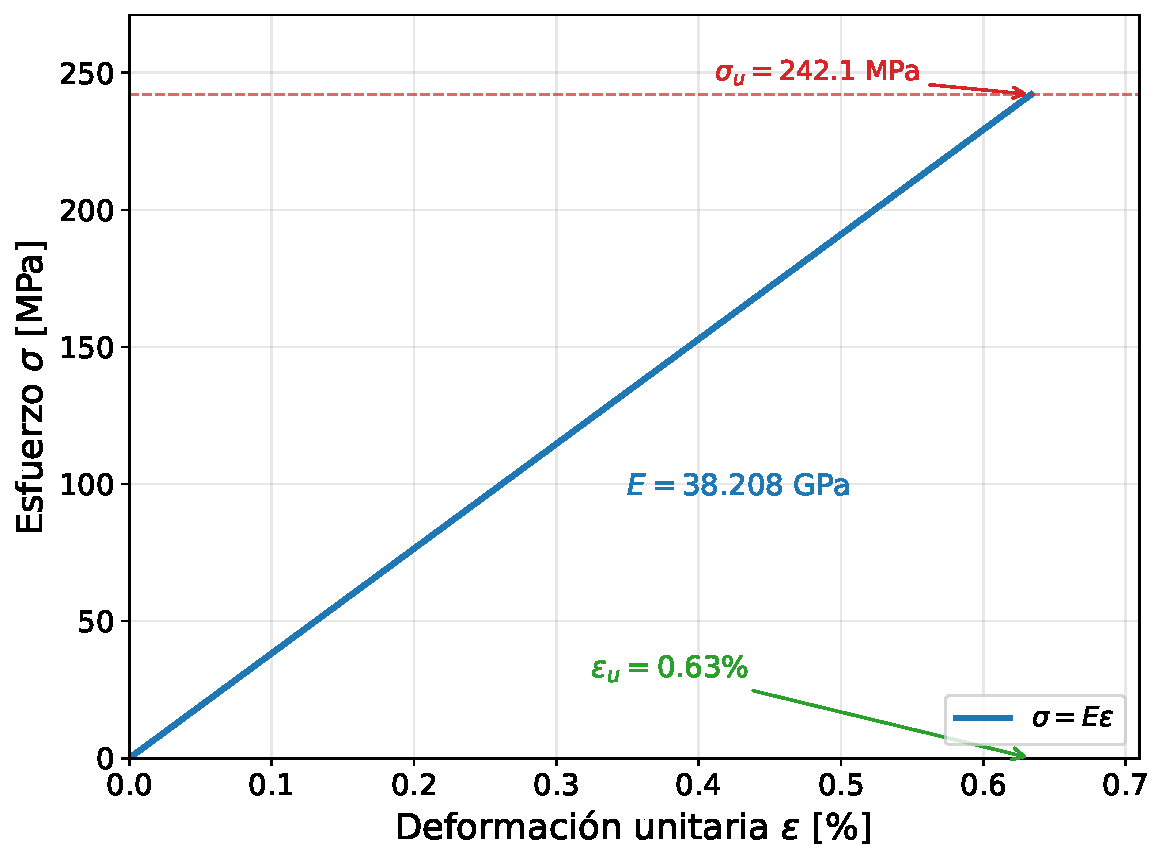
\includegraphics[width=0.65\textwidth]{Figuras/Figuras Metodología/curva_esfuerzo_deformacion.pdf}
    \caption{Curva esfuerzo-deformación del GFRP $\pm 45^\circ$ de la pala, construida a partir de las propiedades entregadas por el fabricante.}
    \label{fig:curva_esfuerzo_deformacion}
\end{figure}

Las propiedades disponibles del laminado son las de la Tabla~\ref{tab:material_pala}: un módulo elástico, un coeficiente de Poisson y una resistencia única, esto es, un conjunto isótropo equivalente. Sobre esa base el material se modela como isótropo lineal. Dos condiciones del análisis hacen consistente esa representación. La primera es que la pala está construida íntegramente con el mismo laminado, de modo que el modelo no debe reproducir desajustes de rigidez entre la piel y el larguero. La segunda es que la verificación de resistencia última emplea el criterio de tensión principal máxima, que compara una tensión escalar con una resistencia única y no requiere descomponer el estado tensional en las direcciones del refuerzo. El alcance de la hipótesis se retoma en las conclusiones.

\subsection{Análisis por modelado de elementos finitos de la pala}
\label{sec:fem}

El análisis estructural de la pala se realiza en el software Ansys. En correlación con los objetivos propuestos, se modela únicamente una pala, excluyendo los struts, la torre y el sistema de flotación del dominio de cálculo. La exclusión del sistema de flotación responde, además, a la falta de datos para modelarlo: el fabricante no entrega su geometría ni sus propiedades, información que resguarda por confidencialidad comercial. La discretización emplea las mismas 24 estaciones adoptadas para instrumentar la pala en QBlade (Sección~\ref{sec:discretizacion}), lo que permite trasladar directamente las cargas sin requerir interpolación entre dominios.

\subsubsection{Condiciones de borde}
\label{sec:condiciones_borde}

La pala se sostiene en los dos puntos en que se conecta a los brazos, situados a $z = 5{,}0$ y $z = 17{,}0$~m sobre la base (Tabla~\ref{tab:geometria_turbina}), que constituyen por tanto sus únicos apoyos. Ambos se representan como empotramientos, esto es, restringiendo los seis grados de libertad, criterio coherente con la rigidez del conjunto brazo-eje frente a la de la pala y con la exclusión de los brazos del dominio de cálculo. La restricción no se impone sobre una arista ni sobre un nodo, sino sobre una superficie de $500 \times 600$~mm en cada conexión, de modo que la reacción se reparte sobre un área finita y no genera la singularidad de tensión que produciría un apoyo puntual. Bajo estas condiciones la pala se comporta como una viga con dos apoyos y un voladizo en cada extremo, configuración que determina las zonas críticas del análisis.

La zona de conexión incorpora además un vendaje de refuerzo de $20$~mm de espesor y $1$~m de longitud, dispuesto concéntricamente alrededor del perímetro de la sección, que reproduce el engrosamiento local del laminado con que se resuelve la introducción de carga en una unión de este tipo.

\subsubsection{Cargas aplicadas}

Las fuerzas aerodinámicas se aplican según el procesamiento de datos específico de cada caso. Además de ellas, se aplican las cargas másicas de origen inercial, que por su naturaleza determinística no requieren extrapolación estadística. Estas no se introducen como fuerzas nodales, sino como aceleraciones globales impuestas sobre la totalidad del modelo: el solucionador las convierte en fuerzas de volumen elemento a elemento, multiplicando la masa de cada elemento por la aceleración prescrita, de modo que la distribución espacial de la carga inercial queda determinada por la distribución de masa del propio modelo. Las aceleraciones que definen estas cargas son:

\begin{itemize}
    \item \textbf{Aceleración de gravedad:} uniforme, dirigida verticalmente hacia abajo y de magnitud $g = 9{,}81$~m/s$^2$.
    \item \textbf{Aceleración centrífuga:} dirigida radialmente hacia afuera, producida por la rotación del rotor y evaluada en la velocidad máxima de rotación $\Omega$ mediante la Ec.~\ref{eq:centrifugal_limit} (Sección~\ref{sec:vtip}). Por tratarse de un H-rotor de palas rectas paralelas al eje, el radio $R$ es constante a lo largo de la envergadura, de modo que la aceleración resulta uniforme en toda la pala y admite imponerse como un único campo global. El valor que corresponde a la consigna de rotación adoptada se presenta en el Capítulo~4.
\end{itemize}

\subsubsection{Discretización de la malla}

La pala se discretiza mediante elementos sólidos tridimensionales de tipo hexaédrico dominante, discretización que \textcite{HAND2021} emplean y validan para el análisis estructural por elementos finitos de palas de \gls{vawt}. El calificativo dominante indica que en las regiones donde la geometría no admite el barrido hexaédrico, como las transiciones de espesor y los encuentros con el larguero, el mallador recurre localmente a elementos de transición.

Para garantizar la independencia de los resultados respecto del tamaño de malla, se realiza un análisis de convergencia variando progresivamente la densidad de elementos hasta que la variación en la tensión principal máxima entre mallas sucesivas sea inferior al $5\%$, umbral establecido en la literatura para análisis de elementos finitos~\parencite{Qin2026} y empleado en estudios de palas eólicas~\parencite{Hameed2015,Boudounit2020}. Este procedimiento elimina la influencia de concentradores de esfuerzos propios de la discretización.

A partir del análisis se obtienen la tensión principal máxima ($\sigma_1$), las deformaciones unitarias y los desplazamientos nodales. La verificación de resistencia última se realiza mediante el criterio de máxima tensión principal, apropiado para materiales compuestos de matriz polimérica con comportamiento frágil~\parencite{Moraras2023}. Al representar el laminado como un sólido homogéneo, la verificación aborda la rotura gobernada por las fibras y no resuelve los mecanismos interlaminares descritos en la Sección~\ref{sec:comportamiento_laminado}. El criterio se aplica comparando $\sigma_{1,\max}$ con la resistencia última factoreada del material, cuyas propiedades mecánicas proporciona el fabricante de la turbina.

\subsubsection{Verificación de estabilidad (pandeo)}
\label{sec:pandeo_met}

La verificación de estabilidad exigida por la Sección 7.6.4 de la norma IEC 61400-1~\parencite{IEC61400-1} se realiza mediante un análisis de pandeo lineal por autovalores (\textit{Eigenvalue Buckling}) en Ansys, según el planteamiento de la Ec.~\ref{eq:pandeo_autovalores} de la Sección~\ref{sec:pandeo_teoria}, acoplado a las soluciones estáticas de ambos casos de carga última (DLC 1.1 y 1.3), de las cuales hereda la malla, las cargas y las condiciones de borde. La simulación entrega el multiplicador de carga (\textit{load multiplier}, $LM$) de cada modo, es decir, el factor por el que deberían amplificarse las cargas aplicadas para alcanzar la inestabilidad elástica, y se extraen los tres primeros modos.

Dado que las cargas aplicadas ya incorporan el factor parcial $\gamma_f$, la condición de verificación se plantea del lado de la resistencia con los mismos factores parciales de la verificación de resistencia última, según la Ec.~\ref{eq:criterio_pandeo}:

\begin{equation}
    LM \geq \gamma_m \cdot \gamma_n = 1{,}30
    \label{eq:criterio_pandeo}
\end{equation}

donde $\gamma_m = 1{,}30$ y $\gamma_n = 1{,}00$ son los factores parciales de resistencia última de la Tabla~\ref{tab:factores_seguridad}. El criterio exige, por tanto, que el modo crítico no se alcance antes de amplificar las cargas de diseño en un $30\%$.

Cabe señalar que el método lineal por autovalores no incorpora imperfecciones geométricas ni efectos no lineales, a los que los cascarones de pared delgada son sensibles, por lo que sus resultados constituyen una cota superior de la carga crítica real (Sección~\ref{sec:pandeo_teoria}).

Junto al caso base, con piel y larguero de $8$~mm, se resuelven dos variantes que acotan el origen del margen obtenido, ambas sobre el caso de carga gobernante y con idénticas condiciones de borde. La primera suprime el larguero interior, con lo que se evalúa la alternativa de fabricación que plantea el fabricante (Sección~\ref{sec:material_pala}). La segunda aumenta el espesor del larguero a $12$~mm, manteniendo la piel en $8$~mm, con lo que se comprueba la sensibilidad del resultado al supuesto adoptado para ese espesor ante la falta de una definición del laminado. Ambas variantes permiten discriminar si la capacidad del conjunto la gobierna el larguero o los paneles de piel, distinción que determina hacia dónde debe dirigirse un eventual refuerzo.


\chapter{Resultados}

Los resultados se presentan siguiendo la secuencia de la metodología expuesta en el Capítulo~3, de modo que cada conjunto de valores se apoya en el anterior. Se parte de la caracterización del emplazamiento (recurso eólico, propiedades termofísicas del aire y rango del número adimencional de Reynolds), que fija las condiciones ambientales de todo el análisis. Sobre esa base se exponen la caracterización aerodinámica del perfil NACA 0018 y las simulaciones aerodinámicas del rotor, de las cuales se obtienen las series temporales de fuerzas sobre la pala. A partir de dichas series se determinan las cargas de diseño de los casos DLC 1.1 y 1.3 y el espectro de fatiga del DLC 1.2, conforme a IEC 61400-1~\parencite{IEC61400-1}; las primeras constituyen la entrada al modelo de elementos finitos. El capítulo cierra con la verificación estructural de la pala, donde las tensiones y deformaciones obtenidas se contrastan con los criterios de resistencia última, estabilidad, deflexión y fatiga que establece la norma.

\section{Caracterización del recurso eólico}
\label{sec:recurso_eolico}

Los resultados de la caracterización del recurso eólico según IEC 61400-1~\parencite{IEC61400-1} se resumen en la Tabla~\ref{tab:viento_vawt}. A partir de los datos del explorador eólico registrados a $z = 5{,}5$~m y extrapolados a la altura del centro del rotor ($z = 21{,}3$~m), según el procedimiento descrito en la Sección~\ref{sec:recurso_metodo}, se obtienen los parámetros de diseño del emplazamiento.

\begin{table}[H]
    \centering
    \caption{Resultados del análisis eólico según estándar IEC 61400.}
    \label{tab:viento_vawt}
    \begin{tabular}{lcc}
        \hline
        \textbf{Parámetro} & \textbf{Símbolo} & \textbf{Valor} \\ \hline
        Velocidad media Anual al Centro del Rotor ($z = 21{,}3$ m) & $V_{ave}$ & $7{,}94$ m/s \\
        Velocidad de referencia & $V_{ref}$ & $39{,}7$ m/s \\
        Intensidad de turbulencia de referencia & $I_{ref}$ & $0{,}12$ \\
        Parámetro de ordenada NTM & $b_{NTM}$ & $5{,}6$ m/s \\
        Clase de emplazamiento (IEC) & --- & II\textsubscript{C} \\ \hline
    \end{tabular}
\end{table}

La velocidad media anual de $7{,}94$~m/s (Figura~\ref{fig:viento_promedio_anual}) presenta una variabilidad reducida durante el período analizado, ya que la desviación relativa de la velocidad media de cada año respecto de $V_{ave}$ no supera el $10\%$ en ninguno de los $38$ años del registro, con un mínimo de $7{,}34$~m/s en 2016 ($-7{,}6\%$) y un máximo de $8{,}47$~m/s en 1994 ($+6{,}7\%$). El ajuste lineal de esos promedios frente al año no muestra, además, una tendencia significativa (pendiente de $0{,}003$~m/s por año, $R^2 = 0{,}01$), lo que respalda tratar el registro histórico completo como representativo del recurso a lo largo de la vida de diseño de $20$ años. La estimación de la turbulencia mediante la Ec.~\ref{eq:charnock_sigma}, con la constante de Charnock de mar abierto, entrega una intensidad de $10{,}5\%$ a $15$~m/s, inferior al umbral $I_{ref} = 0{,}12$ de la categoría C, que resulta así la de menor umbral capaz de envolver la turbulencia del sitio, y es por tanto el valor de $I_{ref}$ que se adopta para el emplazamiento. La clasificación resultante corresponde a Clase II\textsubscript{C} ($37{,}5 \leq V_{ref} < 42{,}5$~m/s, $I_{ref} \leq 0{,}12$), y los parámetros del NTM son los que la norma tabula para esa categoría~\parencite{IEC61400-1}.

\begin{figure}[H]
\centering
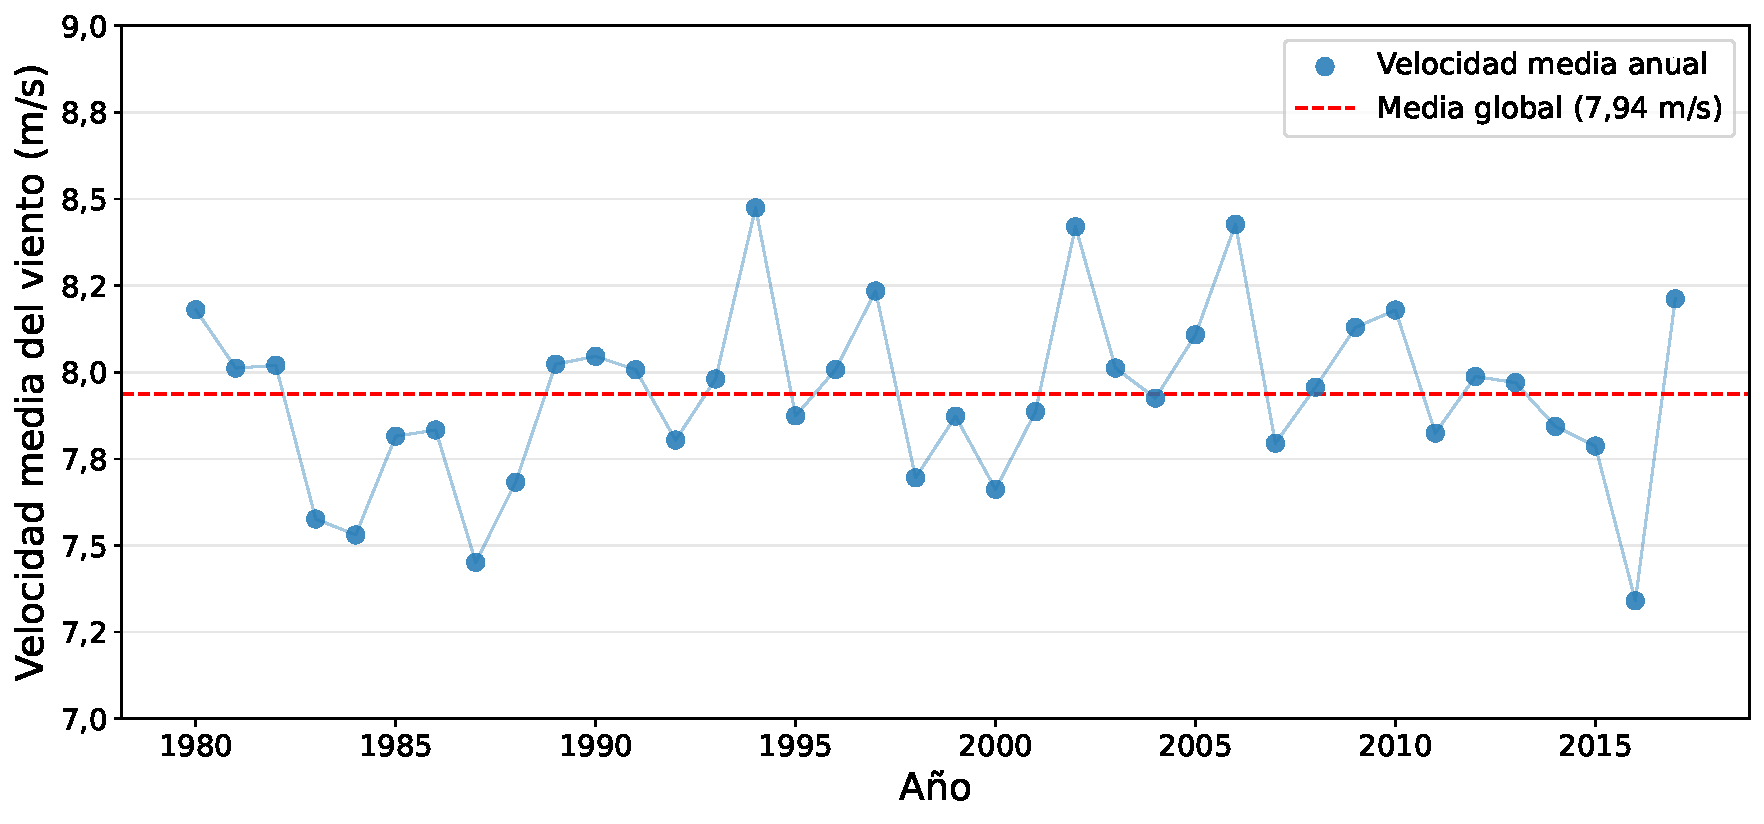
\includegraphics[width=0.7\textwidth]{Figuras/Figuras Resultados/viento_promedio_anual.pdf}
\caption{Velocidad media anual del viento para el periodo 1980--2017.}
\label{fig:viento_promedio_anual}
\end{figure}

La Figura~\ref{fig:viento_promedio_mensual} muestra que los meses de invierno (junio--agosto) presentan velocidades medias superiores a la media anual, mientras que los meses de verano (enero--marzo) registran las velocidades más bajas, con una diferencia estacional cercana al $30\%$.

\begin{figure}[H]
\centering
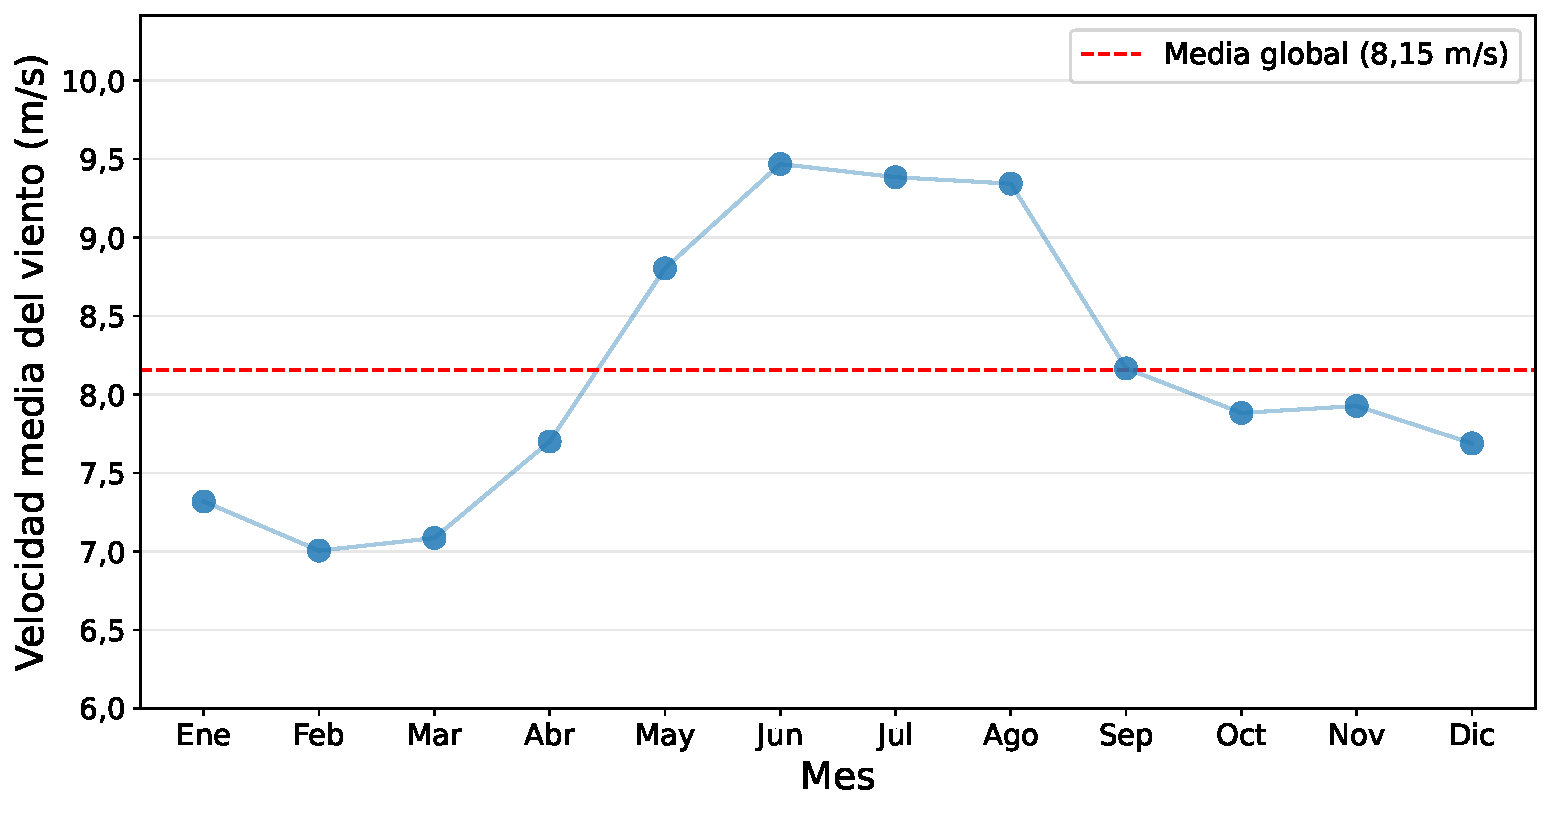
\includegraphics[width=0.7\textwidth]{Figuras/Figuras Resultados/viento_promedio_mensual.pdf}
\caption{Velocidad media mensual del viento para el periodo 1980--2017.}
\label{fig:viento_promedio_mensual}
\end{figure}

La densidad de probabilidad de la velocidad del viento (Figura~\ref{fig:distribucion_viento}) presenta un parámetro de forma $k = 2{,}09$, cercano al caso particular $k = 2$ de la distribución de Rayleigh que la norma adopta como referencia para las clases estándar~\parencite{ennis2018}, y un parámetro de escala $c = 8{,}97$~m/s, ajustados a la altura del centro del rotor, donde la velocidad media resulta en $V_{ave} = 7{,}94$~m/s. El ajuste reproduce la densidad observada con $R^2 = 0{,}970$. Estos dos parámetros reaparecen a lo largo del estudio, ya que la distribución que definen pondera el tiempo de exposición a cada velocidad en el cálculo de fatiga (Sección~\ref{sec:resultados_fatiga}) y entrega la probabilidad de excedencia con que se fija la velocidad de corte.

\begin{figure}[H]
\centering
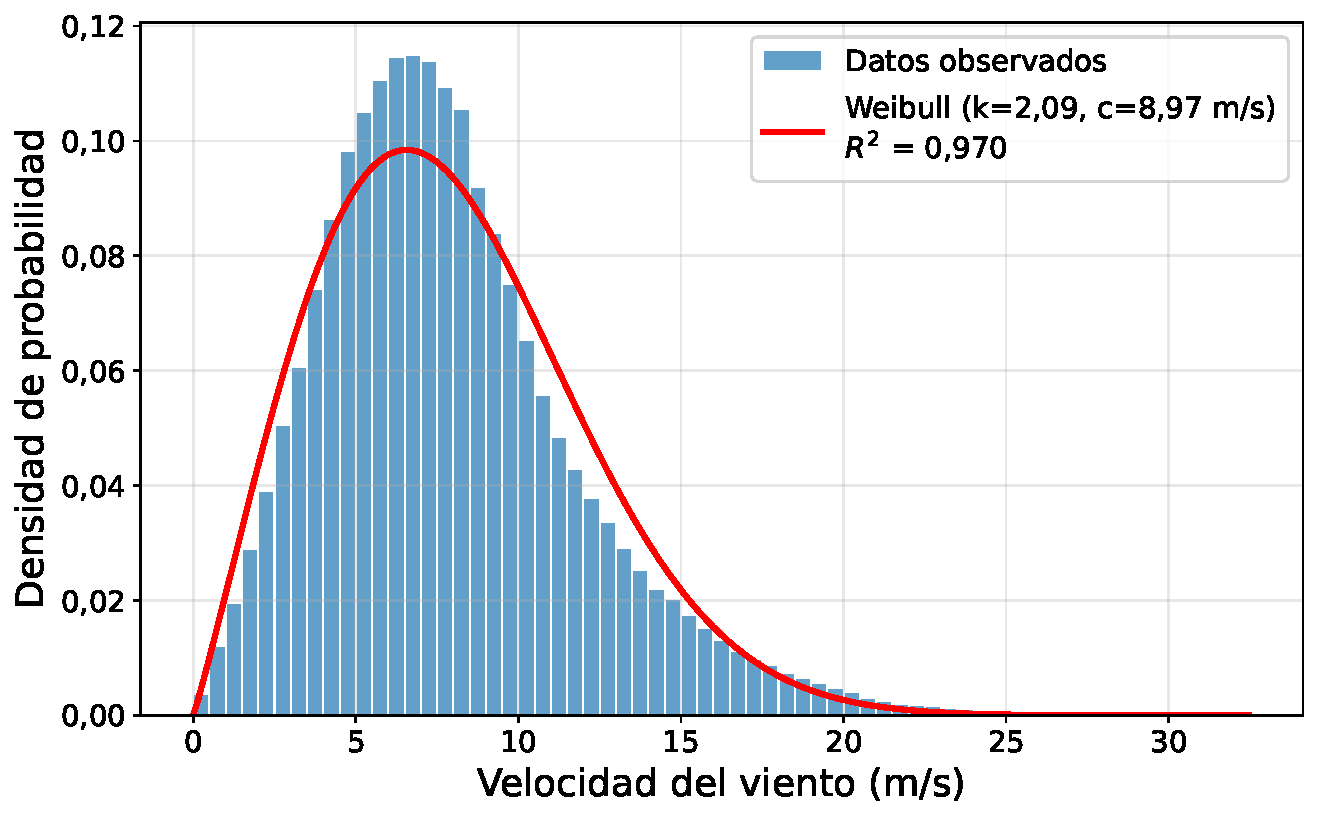
\includegraphics[width=0.7\textwidth]{Figuras/Figuras Resultados/viento_weibull.pdf}
\caption{Densidad de probabilidad y ajuste de Weibull de la velocidad del viento.}
\label{fig:distribucion_viento}
\end{figure}

Con base en esta caracterización, el rango operacional de la turbina se define entre $V_{in} = 2$~m/s y $V_{out} = 25$~m/s. La operación estable a $2$~m/s se verifica mediante las simulaciones LLFVW, que registran producción sostenida y un TSR cercano al óptimo ($C_{p,med} = 0{,}447$, $\lambda = 3{,}88$, Tabla~\ref{tab:curva_potencia}, Sección~\ref{sec:curva_potencia}). El límite superior, adoptado por criterio de diseño (Sección~\ref{sec:control}), tiene un costo marginal en producción, ya que la probabilidad de excedencia del sitio es $P(V > 25\text{ m/s}) = 0{,}02\%$, equivalente a $1{,}75$~h/año, sensiblemente menor a la probabilidad de superar los $20$~m/s, $P(V > 20\text{ m/s}) = 0{,}48\%$ ($42$~h/año). Dado que el coeficiente de potencia decae por debajo de $0{,}06$ para $V \geq 24$~m/s bajo el límite de velocidad de rotación adoptado (Sección~\ref{sec:curva_potencia}), la energía capturable por encima de $25$~m/s resulta despreciable, por lo que las velocidades superiores no se consideran en este estudio.

Las características anteriores del emplazamiento, velocidad media moderada, turbulencia baja y estabilidad interanual sin tendencia de largo plazo, respaldan el uso del registro histórico como representativo del recurso para la estimación de la producción energética.

\section{Caracterización de las propiedades físicas del aire}

Se analizan las temperaturas máximas y mínimas del período 1995--2025, registradas en la estación El Tepual, Puerto Montt (aeropuerto; altitud $85$~m; código DMC $410005$), obtenidas del explorador climático~\parencite{CR2}. Las temperaturas medias mensuales extremas registradas son de 3 \textdegree C para las mínimas y 21 \textdegree C para las máximas (Figura~\ref{fig:climatologia_mensual}).

\begin{figure}[H]
\centering
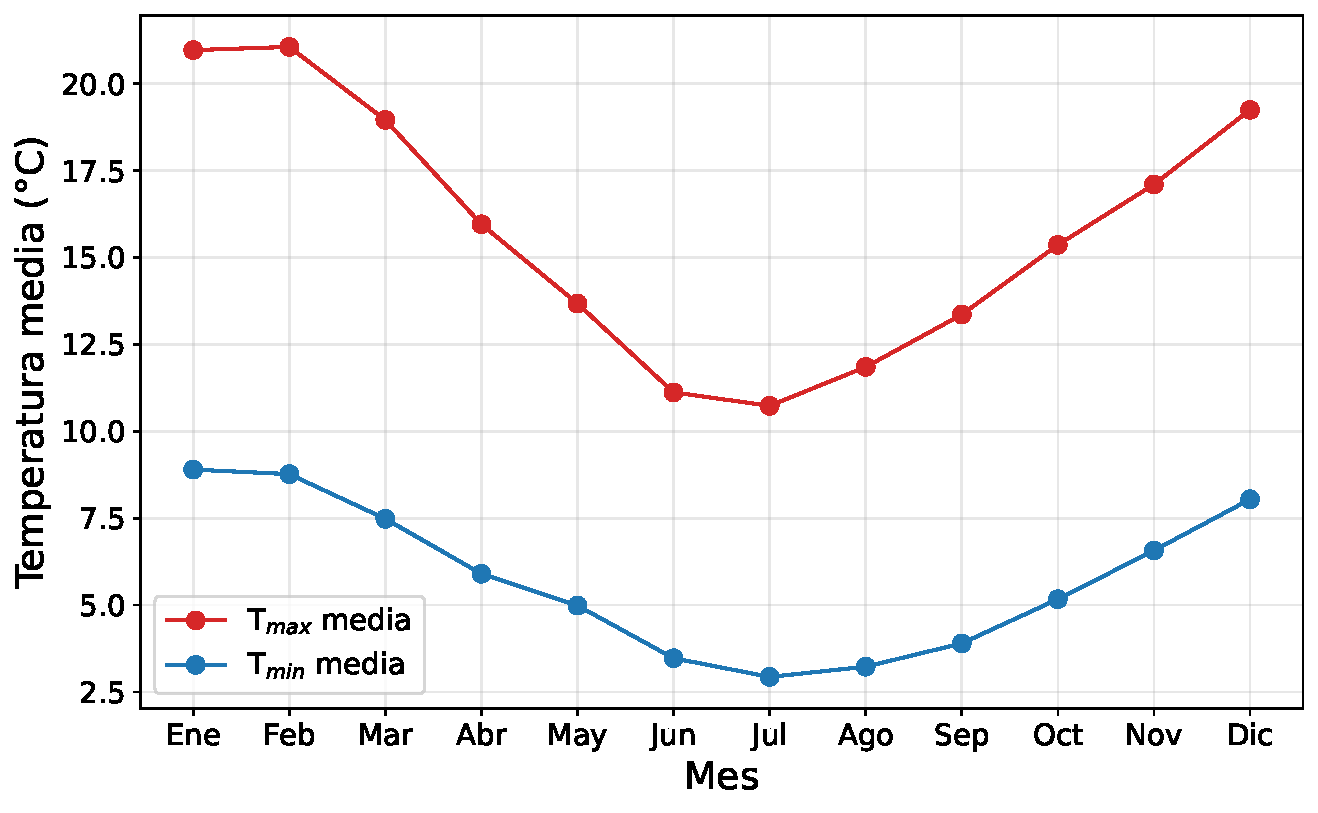
\includegraphics[width=0.6\textwidth]{Figuras/Figuras Resultados/temperatura_climatologia_mensual.pdf}
\caption{Climatología mensual promedio, estación El Tepual, Puerto Montt (1995--2025).}
\label{fig:climatologia_mensual}
\end{figure}

A partir de esta caracterización térmica, se obtienen las propiedades físicas del aire que se resumen en la Tabla~\ref{tab:propiedades_aire}. La variación anual de la viscosidad es inferior al $12\%$, lo que indica que la influencia de la temperatura sobre el número de Reynolds es secundaria respecto a la producida por la variación de la velocidad del viento, efecto que se cuantifica más adelante sobre las fuerzas aerodinámicas (Tabla~\ref{tab:sensibilidad_re}).

\begin{table}[H]
    \centering
    \caption{Propiedades físicas del aire en el emplazamiento, calculadas según las Ecs.~\ref{eq:sutherland}--\ref{eq:visc_cinematica} de la Sección~\ref{sec:propiedades_aire}.}
    \label{tab:propiedades_aire}
    \begin{tabular}{lccc}
        \hline
        \textbf{Propiedad} & \textbf{Símbolo} & \textbf{Valor} & \textbf{Unidad} \\
        \hline
        Viscosidad cinemática mínima & $\nu_{min}$ & $1{,}3535 \times 10^{-5}$ & m$^2$/s \\
        Viscosidad cinemática máxima & $\nu_{max}$ & $1{,}5156 \times 10^{-5}$ & m$^2$/s \\
        Viscosidad cinemática media   & $\bar{\nu}$ & $1{,}4232 \times 10^{-5}$ & m$^2$/s \\
        Densidad media & $\bar{\rho}$ & $1{,}225$ & kg/m$^3$ \\
        \hline
    \end{tabular}
\end{table}

\section{Rango de Reynolds analizado}

La Figura~\ref{fig:reynolds_envelope} presenta la envolvente paramétrica del número de Reynolds en función del ángulo azimutal $\theta$, construida a partir del rango teórico $\lambda \in [2{,}5; 4{,}5]$ y $V \in [2; 25]$~m/s. El $Re_{min} = 2{,}18 \times 10^5$ corresponde a la condición de sotavento a $V = 2$~m/s. La cota superior teórica es $Re_{max} = 5{,}46 \times 10^6$, obtenida a partir de $W_{max} = V_{out} + \Omega R = 70{,}6$~m/s, la simplificación algebraica de la Ec.~\ref{eq:W_theta} para $\theta = 0^\circ$ (Ec.~\ref{eq:W_max}), condición de barlovento en que la velocidad tangencial de la pala se alinea con el viento incidente y ambas magnitudes se suman directamente. Redondeada al millón siguiente, según el criterio de la Sección~\ref{sec:reynolds}, esa cota fija en $6 \times 10^6$ el límite superior adoptado para el cálculo de polares. En cualquier caso, el conjunto de polares calculadas con QFoil ($0{,}35 \times 10^6$ a $6{,}0 \times 10^6$), complementado con las polares experimentales de \textcite{Bianchini2015} para bajo Reynolds ($Re \leq 3 \times 10^5$), cubre completamente las condiciones operacionales simuladas de la turbina.

\begin{figure}[H]
\centering
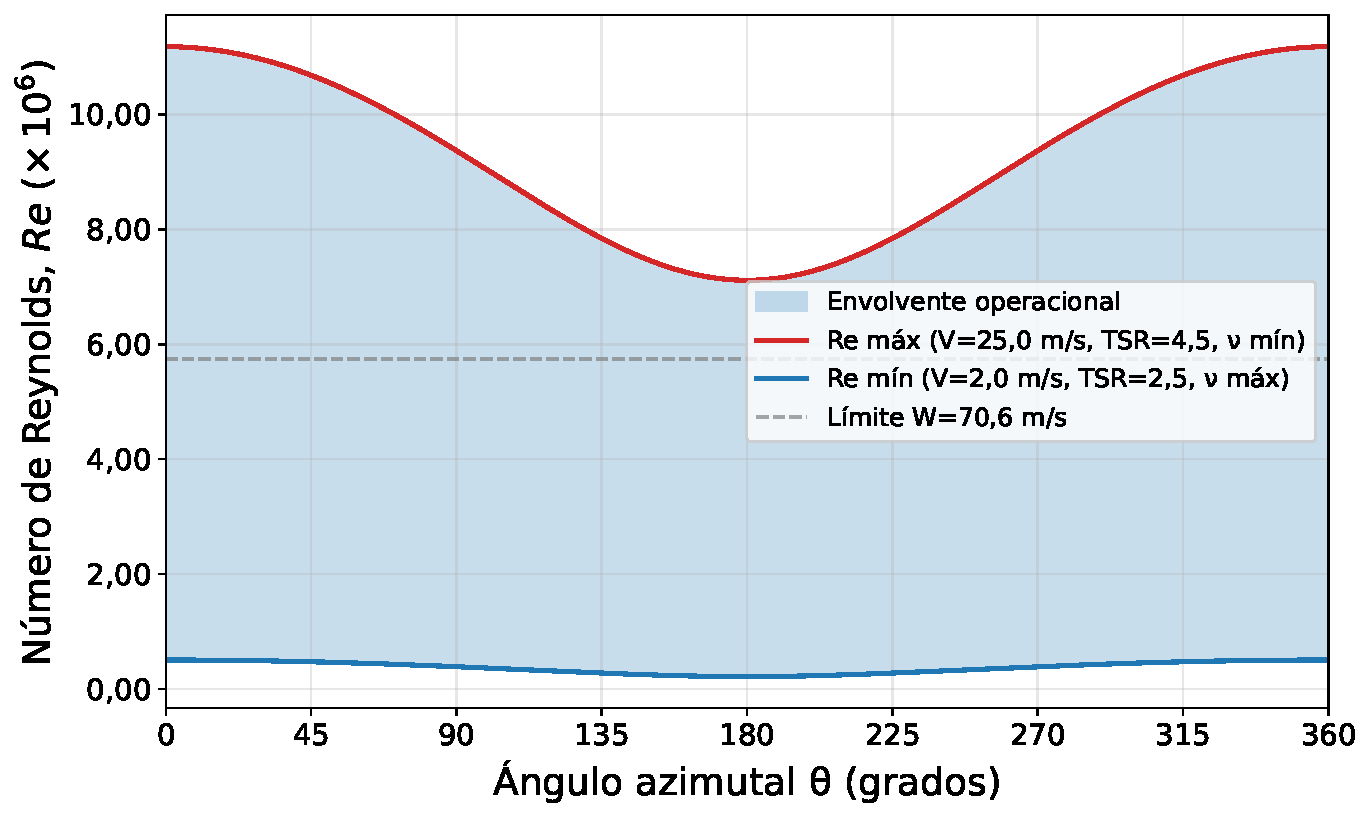
\includegraphics[width=0.75\textwidth]{Figuras/Figuras Resultados/vawt_reynolds_envelope.pdf}
\caption{Envolvente paramétrica del número de Reynolds para el rotor VAWT con perfil NACA 0018.}
\label{fig:reynolds_envelope}
\end{figure}

Esta cobertura resulta particularmente relevante en el extremo superior del rango, donde pequeñas desviaciones en $C_l$ o $C_d$ se amplifican por la dependencia cuadrática de las fuerzas con la velocidad relativa (Ecs.~\ref{eq:fuerza_sustentacion} y~\ref{eq:fuerza_arrastre}).

Esa cobertura absorbe además la incertidumbre que introduce la variabilidad térmica del emplazamiento sobre el Reynolds. Al mantener fija la velocidad relativa $W$, el cociente entre los Reynolds que resultan de evaluar la Ec.~\ref{eq:Re_max_theoretical} con $\nu_{min}$ y con $\nu_{max}$ se reduce al cociente inverso de las viscosidades, según la Ec.~\ref{eq:sensibilidad_re}:

\begin{equation}
    \frac{Re(\nu_{min})}{Re(\nu_{max})} = \frac{Wc/\nu_{min}}{Wc/\nu_{max}} = \frac{\nu_{max}}{\nu_{min}}
    \label{eq:sensibilidad_re}
\end{equation}

de modo que el Reynolds hereda exactamente la misma variación porcentual que la viscosidad. Evaluada en $W_{max} = 70{,}6$~m/s (Sección~\ref{sec:reynolds}), esa variación es de $11{,}98\%$ entre $Re(\nu_{min}) = 5{,}74 \times 10^6$ y $Re(\nu_{max}) = 5{,}12 \times 10^6$, equivalente a $+5{,}2\%$ y $-6{,}1\%$ respecto del $\bar\nu$ adoptado para las simulaciones. Esa magnitud es secundaria frente a la que domina la envolvente de la Figura~\ref{fig:reynolds_envelope}, ya que el rango de $W$ inducido por la velocidad de viento y el TSR analizados abarca un factor de aproximadamente $25$ veces, de $Re_{min} = 2{,}18 \times 10^5$ a $Re_{max} = 5{,}46 \times 10^6$, dos órdenes de magnitud mayor que el efecto térmico.

Las fuerzas de sustentación y arrastre por unidad de envergadura se expresan según las Ecs.~\ref{eq:fuerza_sustentacion} y~\ref{eq:fuerza_arrastre}:

\begin{equation}
    F_L = \frac{1}{2}\rho W^2 c\, C_l(Re,\alpha)
    \label{eq:fuerza_sustentacion}
\end{equation}

\begin{equation}
    F_D = \frac{1}{2}\rho W^2 c\, C_d(Re,\alpha)
    \label{eq:fuerza_arrastre}
\end{equation}

que mantienen $\rho$, $W$ y $c$ fijos frente a este efecto, por lo que su variación porcentual coincide exactamente con la de $C_l$ y $C_d$. La Tabla~\ref{tab:sensibilidad_re} evalúa las polares finales de QFoil ($N_{crit}=7$) entre $Re(\nu_{min})$ y $Re(\nu_{max})$ para ángulos de ataque en régimen adherido, donde $C_l$ varía menos de $0{,}25\%$ y $C_d$ menos de $1{,}2\%$, casi dos órdenes de magnitud menos que el $11{,}98\%$ de variación del propio Reynolds. La influencia de la temperatura sobre las fuerzas predichas resulta, por tanto, despreciable frente a la que ejerce la velocidad del viento, y por extensión sobre el coeficiente de potencia y las cargas estructurales derivadas en las secciones siguientes, lo que refuerza la confiabilidad de las cargas señalada anteriormente.

\begin{table}[H]
    \centering
    \caption{Variación de $C_l$ y $C_d$ del NACA 0018 entre $Re(\nu_{min}) = 5{,}74 \times 10^6$ y $Re(\nu_{max}) = 5{,}12 \times 10^6$, respecto del valor a $\bar\nu$, para ángulos de ataque en régimen adherido.}
    \label{tab:sensibilidad_re}
    \begin{tabular}{ccccc}
        \hline
        \textbf{$\alpha$ (°)} & \textbf{$\Delta C_l(\nu_{min})$} & \textbf{$\Delta C_l(\nu_{max})$} & \textbf{$\Delta C_d(\nu_{min})$} & \textbf{$\Delta C_d(\nu_{max})$} \\
        \hline
        $5$  & $+0{,}11\%$ & $-0{,}13\%$ & $-0{,}33\%$ & $+0{,}55\%$ \\
        $8$  & $+0{,}13\%$ & $-0{,}18\%$ & $-0{,}49\%$ & $+0{,}76\%$ \\
        $10$ & $+0{,}19\%$ & $-0{,}25\%$ & $-0{,}78\%$ & $+0{,}97\%$ \\
        $12$ & $+0{,}18\%$ & $-0{,}21\%$ & $-0{,}96\%$ & $+1{,}14\%$ \\
        \hline
    \end{tabular}
\end{table}

\section{Resultados de la caracterización y extrapolación de perfiles}

Esta sección presenta los resultados de la caracterización aerodinámica del perfil NACA 0018, comenzando por el análisis de sensibilidad que fija el parámetro de transición de QFoil, seguido de las polares finales adoptadas para las simulaciones y de su comparación con datos experimentales.

\subsection{Análisis de sensibilidad al parámetro de transición}

En la Figura~\ref{fig:comparacion_ncrit_250k} se presentan las curvas polares calculadas con QFoil para el perfil NACA 0018 a $Re = 2{,}5 \times 10^5$, considerando los seis valores de $N_{crit}$ simulados, junto con los datos experimentales de \textcite{Bianchini2015} para el mismo número de Reynolds. La figura incluye los coeficientes de determinación $R^2$ del ajuste de $C_l$ respecto a los datos experimentales, evaluados en la región pre-stall ($\alpha \in [-5^\circ, 10^\circ]$), donde el modelo QFoil representa adecuadamente el comportamiento lineal del perfil. Los valores posteriores a la pérdida no son representativos, ya que los códigos de capa límite integral pierden validez cuando la separación se vuelve masiva (Sección~\ref{sec:polares}), y se modelan más adelante en QBlade mediante la extrapolación de Montgomerie de la Sección~\ref{sec:montgomerie_resultados}.

En la curva de sustentación se distinguen tres regiones. Hasta aproximadamente $10^\circ$ el $C_l$ crece de forma prácticamente lineal con el ángulo de ataque y las seis curvas calculadas se superponen con los datos experimentales, lo que se refleja en los valores de $R^2$ cercanos a la unidad. Entre $10^\circ$ y $15^\circ$ la pendiente se aplana y las curvas empiezan a separarse entre sí según el $N_{crit}$ adoptado. La tercera región corresponde a la pérdida, que en los datos experimentales ocurre de forma abrupta en $\alpha = 15{,}6^\circ$, donde el $C_l$ cae de $1{,}03$ a $0{,}49$, mientras que las curvas de QFoil no reproducen esa caída y siguen creciendo hasta $1{,}06$ en $\alpha = 20^\circ$ con $N_{crit} = 7$. La pérdida aparece por tanto antes en los datos experimentales que en las polares calculadas, lo que es esperable en esta etapa, ya que la figura corresponde a la salida directa de QFoil, todavía sin el ajuste de pérdida profunda que se calibra en la Sección~\ref{sec:montgomerie_resultados}.

La elección de $N_{crit}$ tiene un efecto directo sobre la predicción de cargas aerodinámicas. Un valor bajo ($N_{crit} = 4$) fuerza la transición temprana de capa límite, lo que reduce el $C_l$ máximo y subestima las cargas en la zona de stall. Por el contrario, un valor alto ($N_{crit} \geq 11$) retrasa la transición, permitiendo que el flujo permanezca laminar más allá de lo físicamente realista en un entorno operacional, ya que ese rango corresponde a flujos prácticamente libres de perturbaciones (Tabla~\ref{tab:ncrit_values}), y produce una sobrestimación creciente de $C_l$. Ambos efectos son los que documenta \textcite{drela1989xfoil} para el criterio $e^N$, descrito en la Sección~\ref{sec:polares}, y los que se observan en la figura. El valor $N_{crit} = 7$ se sitúa dentro del rango correspondiente a túnel de viento turbulento según la documentación de Xfoil~\parencite{drela1989xfoil}, condición más representativa del ambiente marino en que opera la turbina que los valores $N_{crit} \geq 9$ (túnel de viento limpio o promedio), y es el que mejor reproduce los datos experimentales en la región pre-stall ($R^2 = 0{,}9950$). Por estas razones, $N_{crit} = 7$ es seleccionado como parámetro de configuración para todas las simulaciones aerodinámicas.

\begin{figure}[H]
\centering
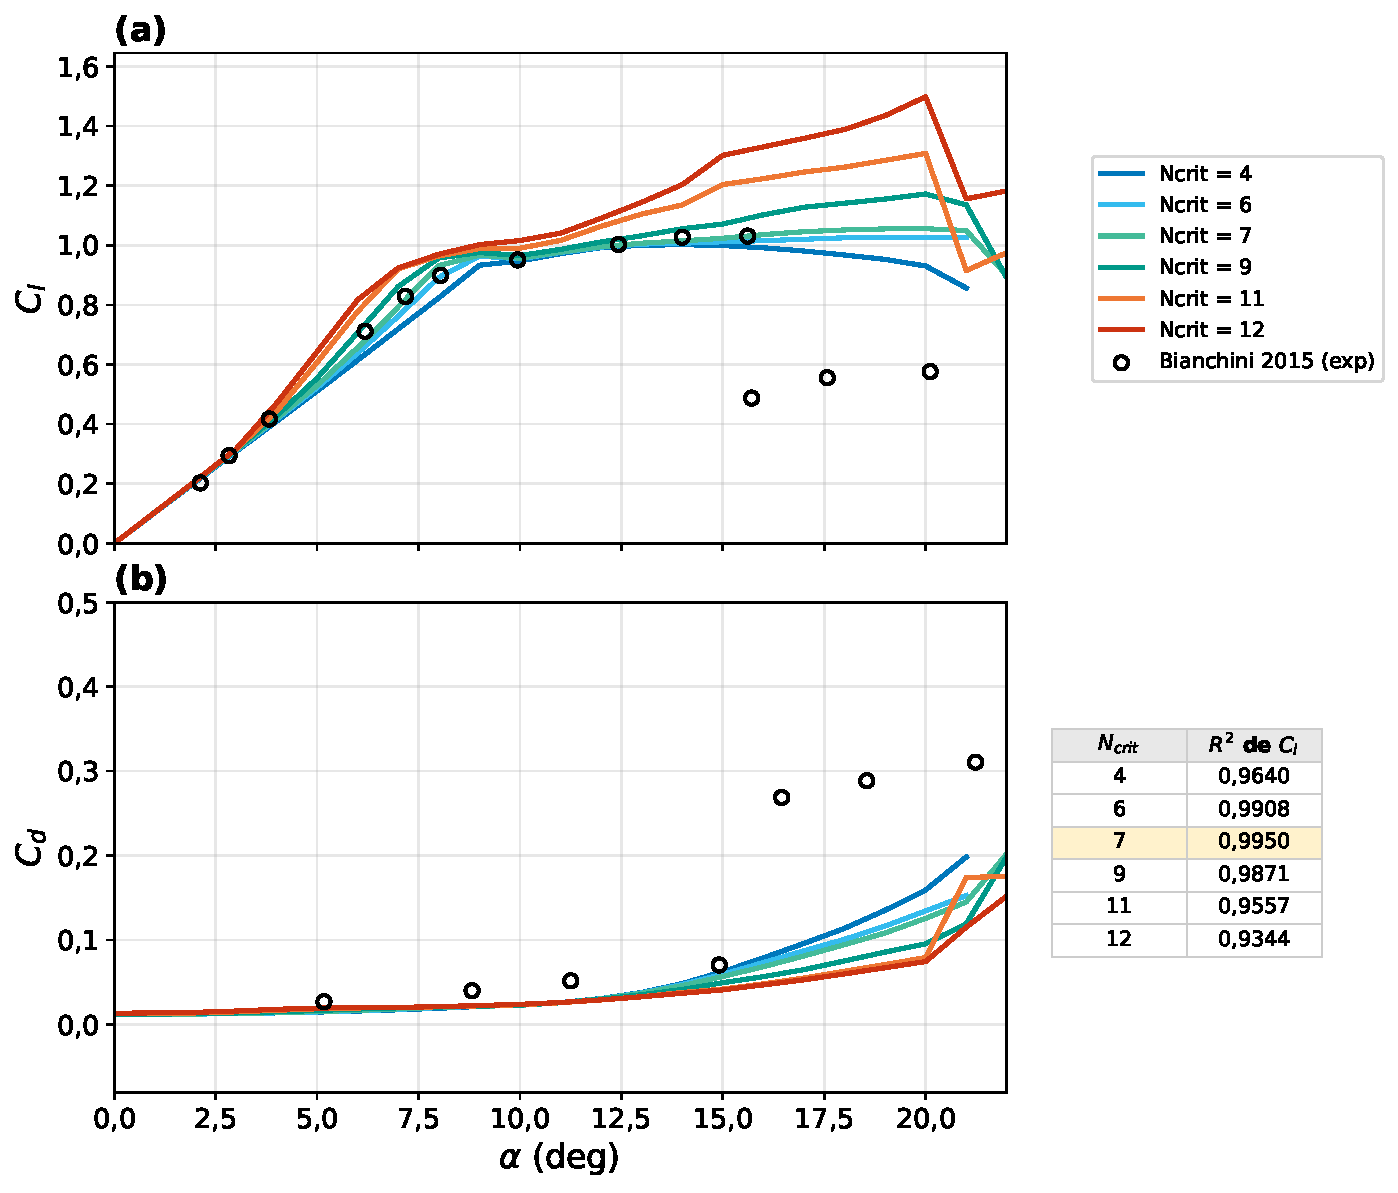
\includegraphics[width=0.9\textwidth]{Figuras/Figuras Resultados/comparacion_vs_experimental_250k.pdf}
\caption{Comparación de polares del perfil NACA 0018 para distintos valores del criterio de transición, $Re = 2{,}5 \times 10^5$: (a) Sustentación y (b) Arrastre.}
\label{fig:comparacion_ncrit_250k}
\end{figure}

\subsection{Polares calculadas}

Las curvas polares calculadas con QFoil para 42 números de Reynolds entre $Re = 0{,}35 \times 10^6$ y $6 \times 10^6$ para el perfil NACA 0018 se presentan en las Figuras~\ref{fig:naca_cl} y~\ref{fig:naca_cd}. El incremento del $38\%$ en $C_{l,max}$ a lo largo del rango de Reynolds, desde $1{,}05$ hasta $1{,}45$, es esperable, ya que a mayor número de Reynolds la capa límite dispone de más energía cinética para resistir el gradiente adverso de presión, retrasando la separación~\parencite{White2006,Anderson2016}. Simultáneamente, la disminución del coeficiente de arrastre en la región pre-stall refleja la reducción del espesor relativo de la capa límite~\parencite{White2006}. El ángulo de stall se mantiene aproximadamente constante en $14^\circ$--$15^\circ$, comportamiento característico de perfiles simétricos NACA de la serie 00XX a números de Reynolds moderados, donde la separación está dominada por el gradiente de presión más que por efectos viscosos~\parencite{Anderson2016}.

\label{sec:montgomerie_resultados}Estas curvas ya incorporan la extrapolación angular a todo el rango que recorre la pala en una revolución completa ($360^\circ$), mediante el modelo de \textcite{montgomerie2004methods} configurado en QBlade con los criterios descritos en la Sección~\ref{sec:extrapolacion_polares}. El coeficiente de arrastre a 90° se fija en $C_{d90} = 1{,}83$ a partir de los datos experimentales de \textcite{Bianchini2015} para el perfil NACA 0018 a $Re = 2{,}5 \times 10^5$.

\begin{figure}[H]
\centering
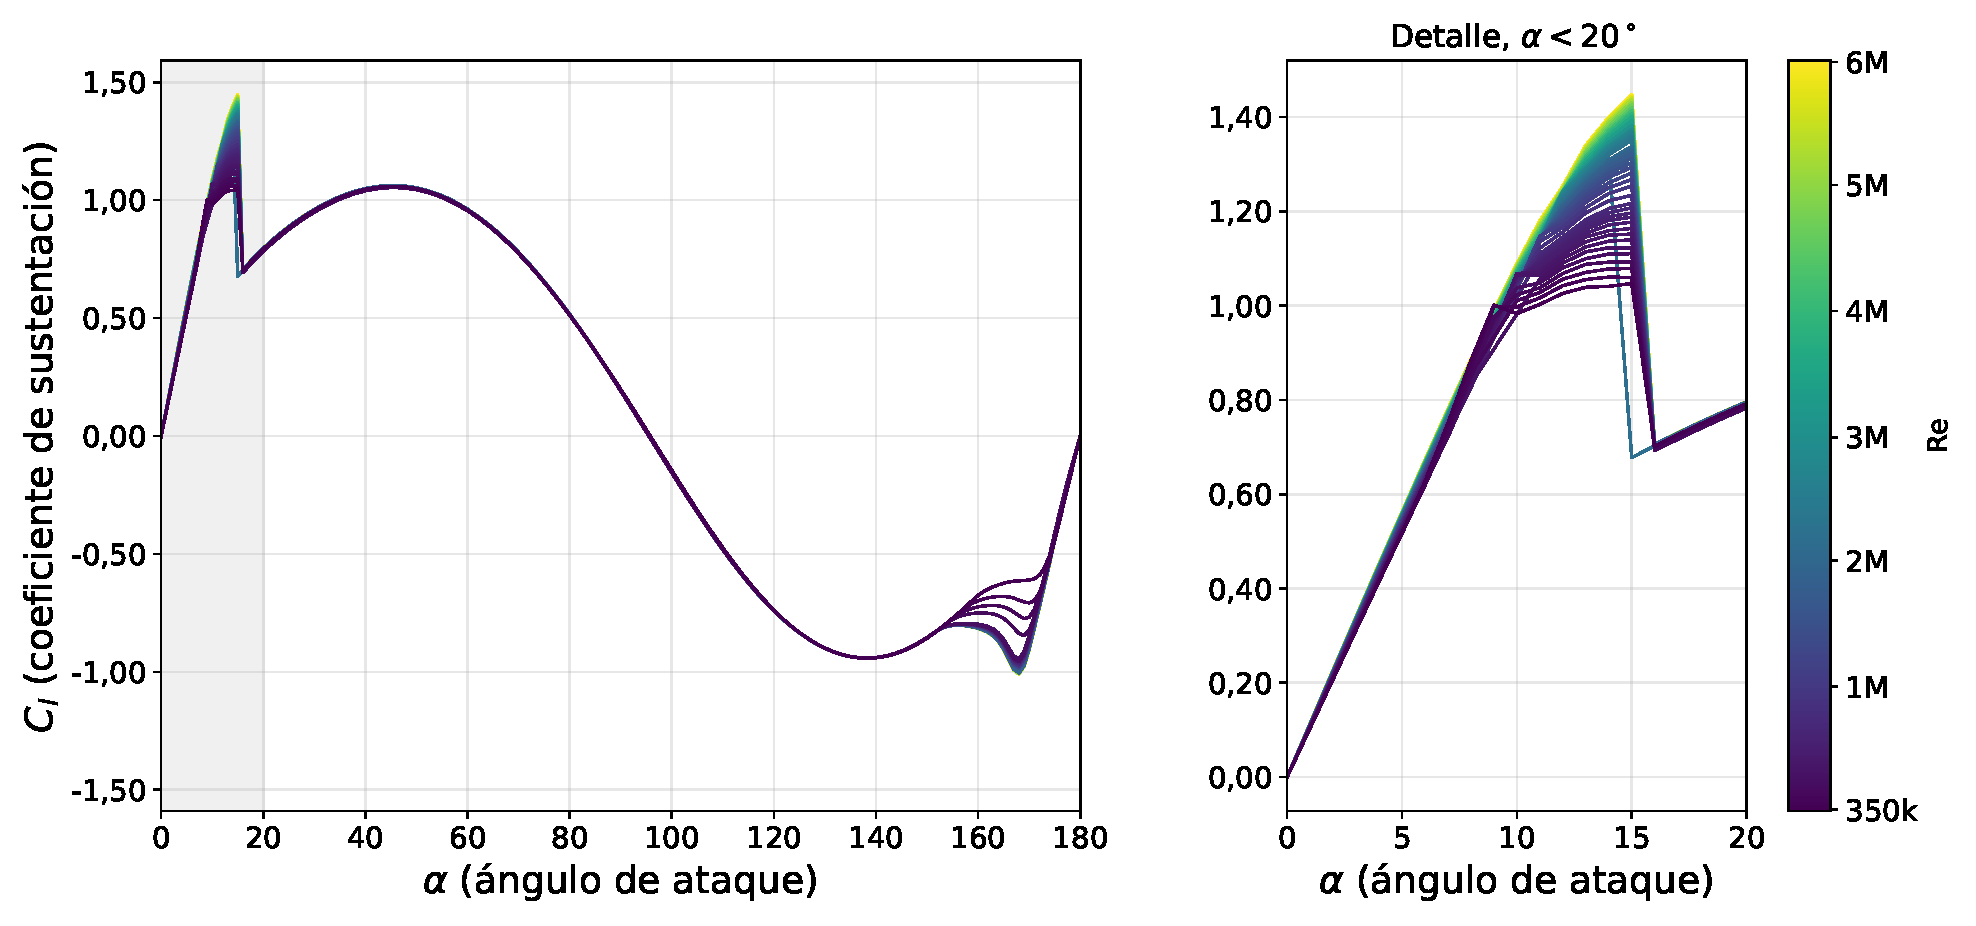
\includegraphics[width=1\textwidth]{Figuras/Figuras Resultados/NACA0018_CL_vs_AoA.pdf}
\caption{Coeficiente de sustentación sobre $\alpha$ del perfil NACA 0018 para diferentes números de Reynolds, $N_{crit}=7$, obtenido mediante QFoil con extrapolación de Montgomerie.}
\label{fig:naca_cl}
\end{figure}

\begin{figure}[H]
\centering
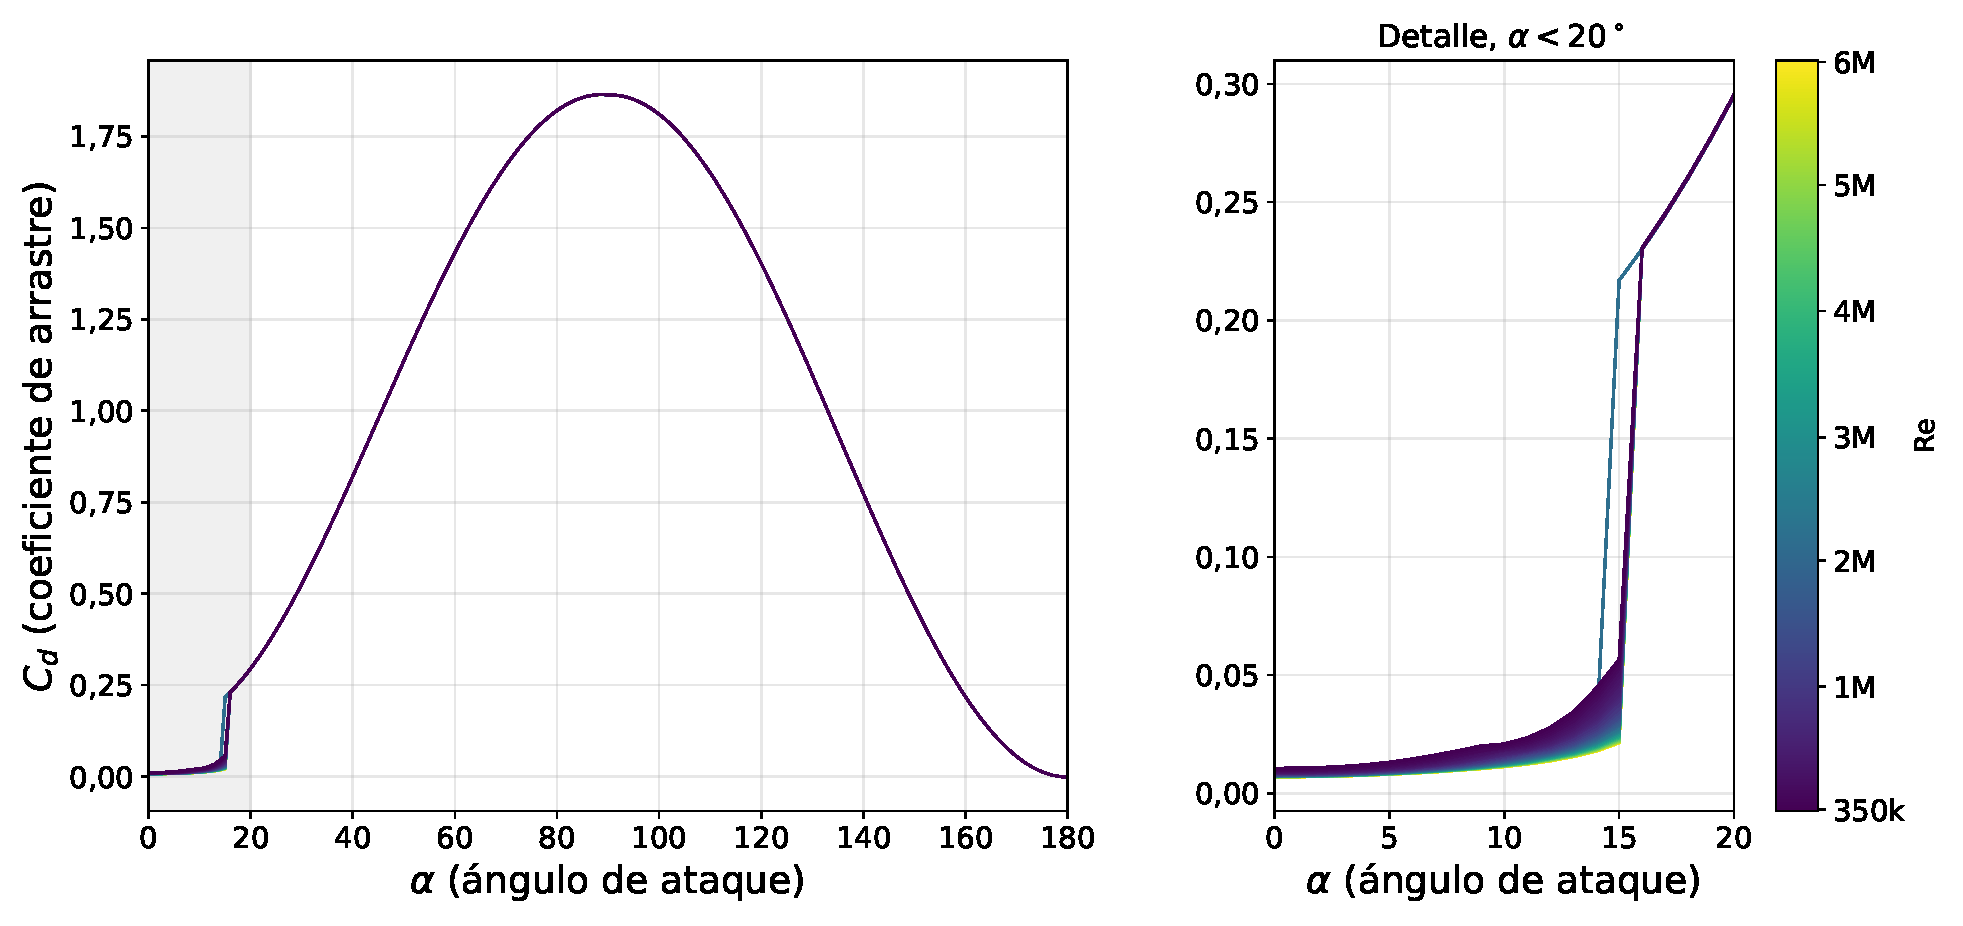
\includegraphics[width=1\textwidth]{Figuras/Figuras Resultados/NACA0018_CD_vs_AoA.pdf}
\caption{Coeficiente de arrastre sobre $\alpha$ del perfil NACA 0018 para diferentes números de Reynolds, $N_{crit}=7$, obtenido mediante QFoil con extrapolación de Montgomerie.}
\label{fig:naca_cd}
\end{figure}

\subsection{Comparación con datos experimentales}

La Figura~\ref{fig:sheldahl_bianchini_qfoil} presenta la comparación entre tres fuentes independientes de datos aerodinámicos para el perfil NACA 0018 en el rango $0^\circ$ a $180^\circ$: las curvas de \textcite{Sheldahl1981}, los datos experimentales de \textcite{Bianchini2015} para $Re = 6 \times 10^4$ a $3 \times 10^5$, y cinco polares representativas calculadas con QFoil ($N_{crit} = 7$) desde $Re = 3{,}5 \times 10^5$ hasta $Re = 5 \times 10^6$. La coincidencia entre las tres fuentes en las zonas de solapamiento de Reynolds es estrecha en la región pre-stall, donde QFoil se desvía de Bianchini menos de un $3\%$ en $C_l$ para $\alpha \geq 8^\circ$, mientras que Sheldahl se aparta hasta un $13\%$, coherente con las deficiencias de esa base de datos histórica señaladas en la Sección~\ref{sec:caracterizacion_aero}. En la región de pérdida profunda, entre $150^\circ$ y $180^\circ$, las diferencias entre Sheldahl y Bianchini alcanzan hasta $0{,}33$ en $C_l$, magnitud comparable a las discrepancias que los propios \textcite{Bianchini2015} reportan en esa misma zona angular al contrastar sus mediciones con sus simulaciones CFD (Sección~\ref{sec:caracterizacion_aero}). Esta coincidencia constituye una validación cruzada entre un método computacional (panel con capa límite integral), datos experimentales recientes y la referencia histórica del perfil. Las polares de Bianchini cubren el rango de bajo Reynolds ($Re \leq 3 \times 10^5$) donde QFoil no alcanza convergencia, complementando así el conjunto de datos requerido para las simulaciones en todo el rango operacional de la turbina.

\begin{figure}[H]
\centering
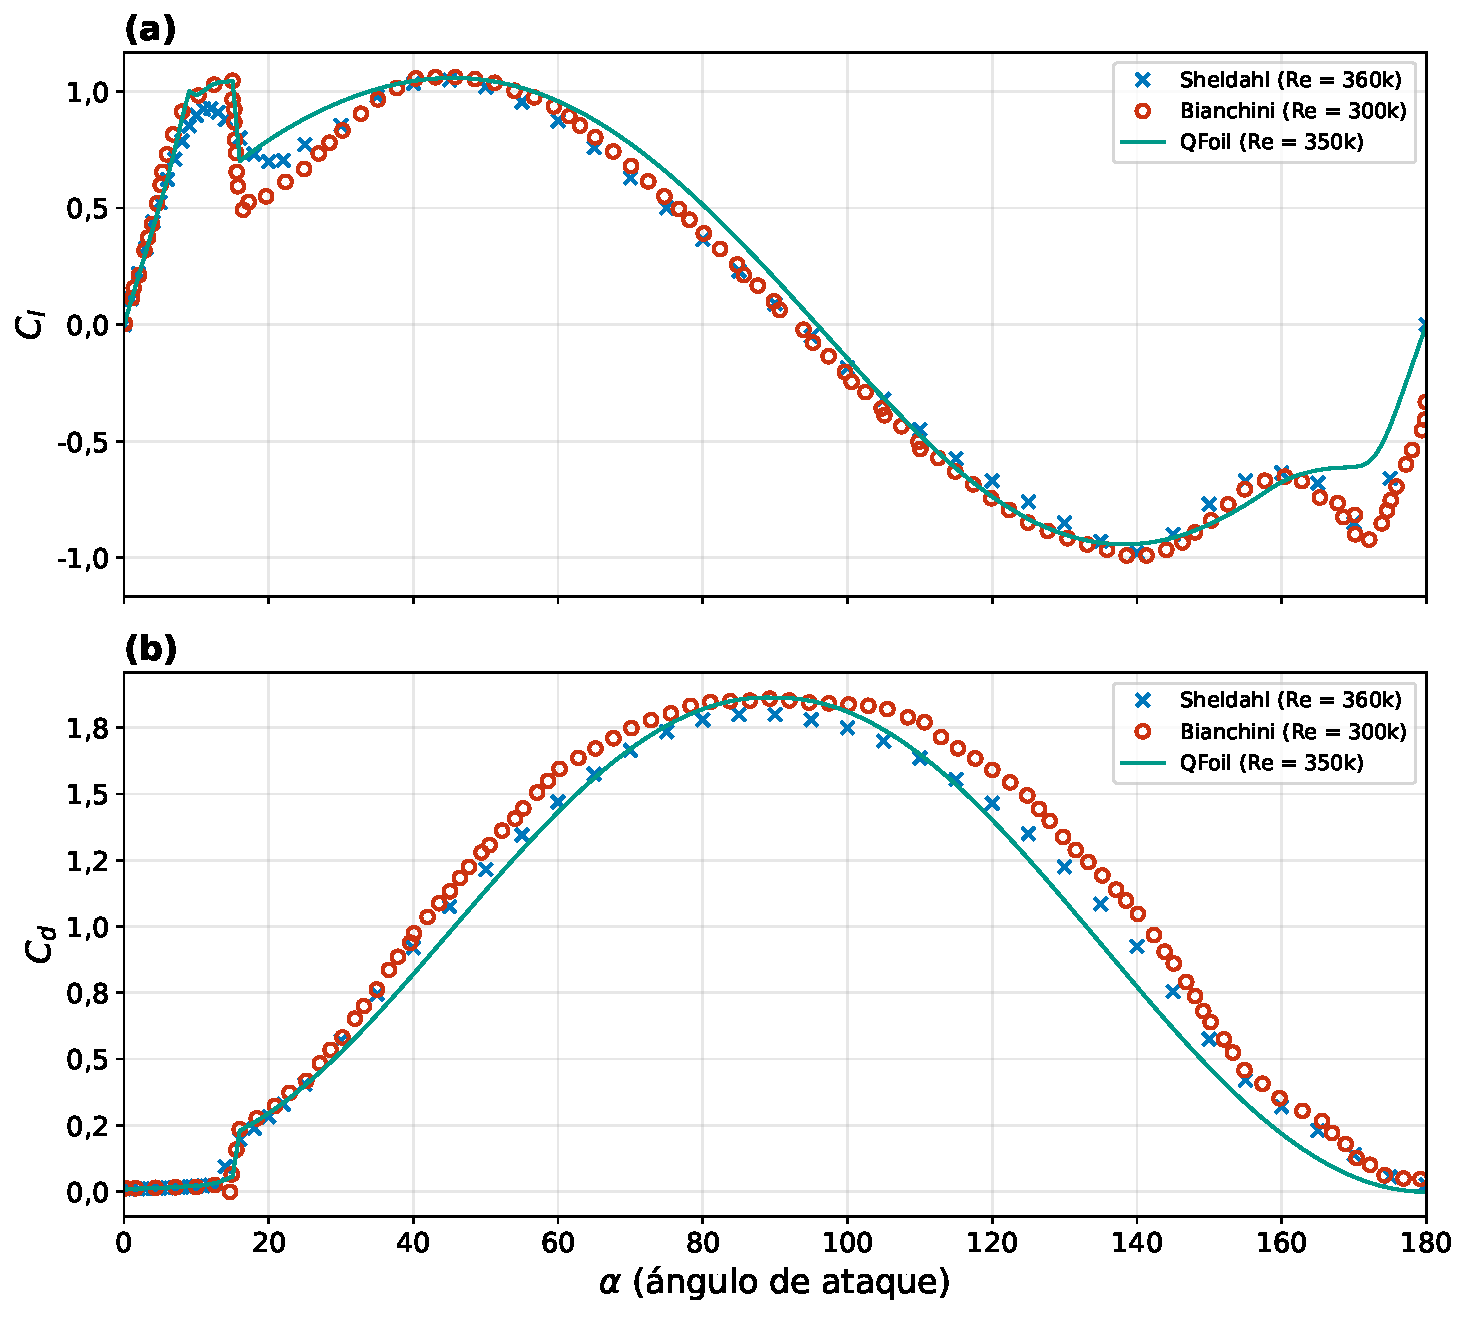
\includegraphics[width=0.85\textwidth]{Figuras/Figuras Resultados/Sheldahl_vs_Bianchini_vs_QFoil.pdf}
\caption{(a) Coeficiente de sustentación $C_l$ y (b) coeficiente de arrastre $C_d$ del perfil NACA 0018, comparando \textcite{Sheldahl1981}, \textcite{Bianchini2015} y QFoil.}
\label{fig:sheldahl_bianchini_qfoil}
\end{figure}

Una vez calibrado el modelo aerodinámico del perfil, la siguiente etapa consiste en caracterizar el desempeño del rotor completo. Antes de ejecutar las simulaciones aerodinámicas de alta fidelidad (LLFVW), se realiza un barrido paramétrico mediante DMST para identificar la relación de velocidad de punta que maximiza la extracción de potencia. El $\lambda_{opt}$ así obtenido se utiliza como condición de referencia para la estrategia de control en las simulaciones LLFVW definitivas.

\section{Relación de velocidad de punta óptima}
\label{sec:tsr_optimo}

La Figura~\ref{fig:dmst_cp_vs_tsr} presenta las curvas TSR vs $C_p$ obtenidas mediante DMST para el rango de velocidades operacionales entre $V_{in} = 2$ m/s y $V_{out} = 25$ m/s. El valor máximo de $C_p$ se alcanza a un $\lambda_{opt} = 3{,}80$, con un $C_{p,max} = 0{,}5736$. Este valor supera el rango validado experimentalmente para configuraciones H-Darrieus ($0{,}35$--$0{,}45$)~\parencite{Essahraoui2026}, en aproximadamente un $27{,}5\%$ sobre el límite superior del rango, sobreestimación sistemática que corresponde a la limitación del método DMST descrita en la Sección~\ref{sec:metodos_aerodinamicos}~\parencite{Essahraoui2026,Islam2008}.

\begin{figure}[H]
    \centering
    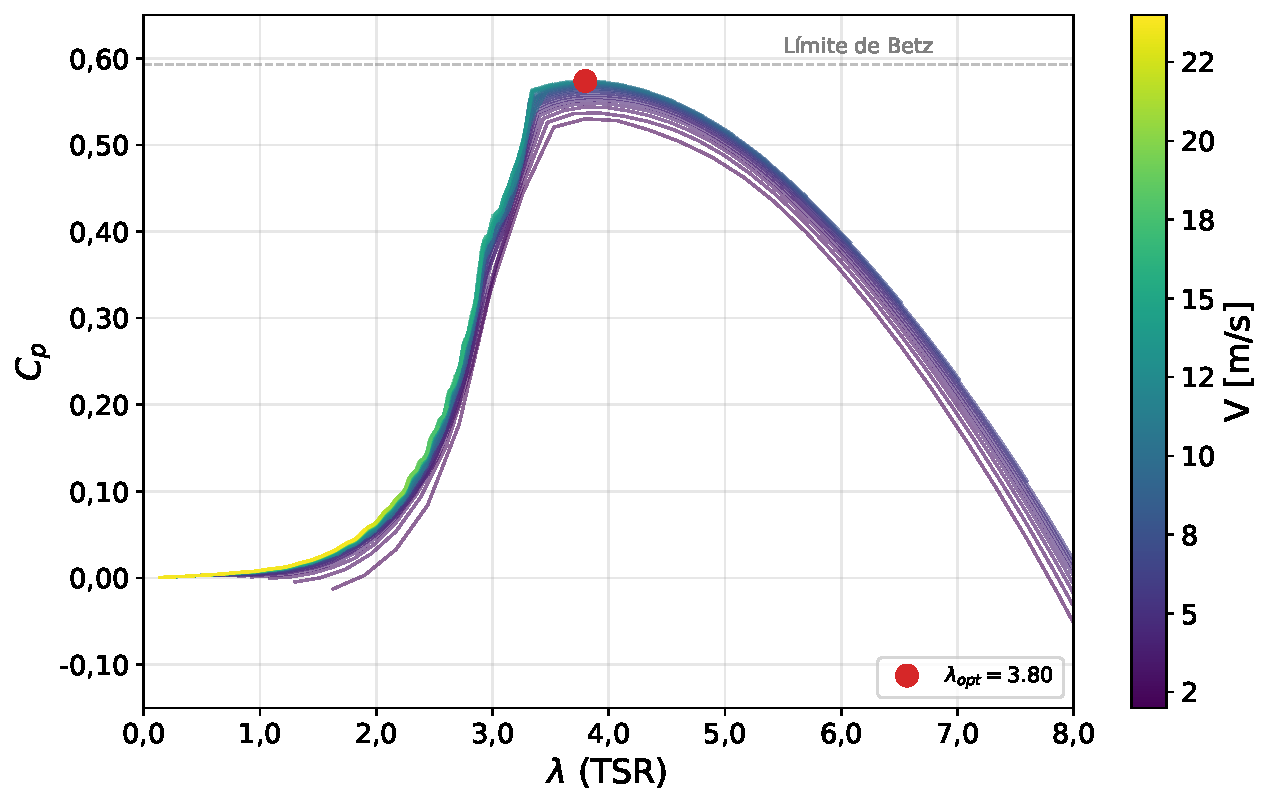
\includegraphics[width=0.75\textwidth]{Figuras/Figuras Resultados/dmst_cp_vs_tsr.pdf}
    \caption{Curvas TSR vs $C_p$ obtenidas mediante DMST para el rango operacional de velocidades de viento, coloreadas según $V$.}
    \label{fig:dmst_cp_vs_tsr}
\end{figure}

La posición del óptimo, en cambio, cuenta con un respaldo independiente del método, ya que la solidez del rotor, $\sigma = Nc/R = 0{,}3184$, se sitúa dentro del rango $0{,}25$--$0{,}35$ que \textcite{Essahraoui2026} reportan como óptimo para H-rotores de tres palas con perfiles simétricos NACA, a partir de los resultados de \textcite{Subramanian2017}, si bien los propios autores advierten que dicho óptimo se desplaza con el perfil, el número de Reynolds y el TSR objetivo. Como se establece en la Sección~\ref{sec:solidez}, este parámetro permite aproximar la posición del máximo de $C_p$ en función del TSR, ya que rotores de baja solidez operan a TSR elevados ($\lambda > 4$) y rotores de alta solidez lo hacen a TSR bajos ($\lambda \approx 2$--$3$). La solidez del rotor estudiado es intermedia entre ambos regímenes, por lo que cabe esperar que su $\lambda_{opt}$ también lo sea, situado entre esos dos extremos; el valor obtenido mediante el barrido DMST, $\lambda_{opt} = 3{,}80$, cae precisamente en ese intervalo intermedio. Esta correspondencia constituye una verificación independiente del resultado, porque la solidez es un parámetro puramente geométrico que no depende del método aerodinámico con que se simula el rotor, de modo que la posición del óptimo que predice, a partir de la relación empírica documentada en la literatura, no hereda el sesgo del DMST señalado en el párrafo anterior. Que ambas vías, la curva TSR vs $C_p$ del barrido DMST y la relación solidez-TSR de la literatura, apunten a la misma posición del óptimo respalda el valor $\lambda_{opt} = 3{,}80$ con independencia de esas limitaciones, aunque estas sí afecten la magnitud de $C_{p,max}$ estimada, como se señala más arriba. Sobre esta base, dicho valor se adopta como TSR de referencia para las simulaciones LLFVW.

Con el \gls{tsr} determinado queda fijada también la consigna de velocidad máxima de rotación. Aplicando el criterio de la Sección~\ref{sec:criterio_rotacion} con $\lambda = 3{,}80$ y la velocidad de viento nominal de $12$~m/s se obtiene la Ec.~\ref{eq:omega_diseno}:

\begin{equation}
    \Omega = \frac{\lambda \, V}{R} = \frac{3{,}8 \times 12}{10{,}365} = 4{,}398\ \text{rad/s} = 42{,}0\ \text{rpm}
    \label{eq:omega_diseno}
\end{equation}

El mismo criterio, aplicado a la T1-turbine ($R = 13$~m), reproduce su límite documentado de $33$~rpm con un error del $1{,}5\%$~\parencite{Mollerstrom2017}, lo que respalda la consigna adoptada. La velocidad de punta que de ella resulta, $V_{tip} = \Omega R = 45{,}6$~m/s, equivale a $\lambda V$ y es por tanto independiente del radio, por lo que coincide con la que se obtiene para la T1-turbine a partir de los parámetros de la Tabla~\ref{tab:t1_params}.

\section{Simulación aerodinámica de la turbina}
\label{sec:curva_potencia}

Con el TSR óptimo determinado y las polares validadas, se procede a la simulación aerodinámica del rotor. A diferencia del barrido DMST, que opera sobre promedios estacionarios, las simulaciones LLFVW resuelven la interacción dinámica entre el campo de viento turbulento y la estela tridimensional que el rotor genera~\parencite{marten2019qblade}.

Los parámetros operacionales de la Tabla~\ref{tab:curva_potencia} corresponden al promedio temporal de cada una de las 72 simulaciones LLFVW (Sección~\ref{sec:velocidades_simulacion}), descartado el transitorio inicial, y promediado a su vez sobre las $6$ semillas por velocidad de viento.

\begin{table}[H]
    \centering
    \caption{Parámetros operacionales promedio de la turbina por velocidad de viento ($\Delta\theta = 5^\circ$, $N = 6$ semillas por velocidad).}
    \label{tab:curva_potencia}
    \begin{tabular}{lcccc}
        \hline
        $V$ (m/s) & RPM & TSR & $P_{med}$ (kW) & $C_{p,med}$ \\
        \hline
        $2$  & $6{,}7$  & $3{,}882$ & $1{,}0$    & $0{,}447$ \\
        $4$  & $13{,}6$ & $3{,}853$ & $8{,}5$    & $0{,}452$ \\
        $6$  & $20{,}0$ & $3{,}734$ & $26{,}3$   & $0{,}438$ \\
        $8$  & $26{,}6$ & $3{,}701$ & $61{,}7$   & $0{,}431$ \\
        $10$ & $33{,}3$ & $3{,}667$ & $121{,}4$  & $0{,}421$ \\
        $12$ & $39{,}5$ & $3{,}698$ & $201{,}5$  & $0{,}432$ \\
        $14$ & $42{,}0$ & $3{,}078$ & $349{,}8$  & $0{,}437$ \\
        $16$ & $42{,}0$ & $2{,}689$ & $485{,}0$  & $0{,}422$ \\
        $18$ & $42{,}0$ & $2{,}391$ & $503{,}4$  & $0{,}327$ \\
        $20$ & $42{,}0$ & $2{,}152$ & $423{,}5$  & $0{,}205$ \\
        $22$ & $42{,}0$ & $1{,}956$ & $369{,}3$  & $0{,}137$ \\
        $24$ & $42{,}0$ & $1{,}793$ & $336{,}3$  & $0{,}094$ \\
        \hline
    \end{tabular}
\end{table}

La progresión de la velocidad de rotación confirma el funcionamiento de la estrategia de control y delimita dos regímenes de operación. Por debajo de $12$~m/s la ley $K$-$\omega^2$ acelera el rotor de forma aproximadamente proporcional al viento~\parencite{Johnson2006}, con lo que el TSR se mantiene entre $3{,}67$ y $3{,}88$, en torno al $\lambda_{opt} = 3{,}80$ de diseño. A partir de $14$~m/s la rotación alcanza su límite de $42$~rpm y permanece en él, mientras el TSR decae hasta $1{,}79$ a $24$~m/s, alejando el punto de operación del óptimo aerodinámico.

Estas simulaciones permiten además verificar a posteriori la validez de las polares empleadas, ya que el número de Reynolds máximo que registran, $Re_{max} = 5{,}94 \times 10^6$ a $V = 24$~m/s, es coherente con la cota teórica de $5{,}46 \times 10^6$ de la Sección~\ref{sec:reynolds}, y la diferencia proviene de las fluctuaciones instantáneas de velocidad inducidas por la turbulencia. Ambos valores quedan cubiertos por el rango de polares adoptado, por lo que en ningún instante se extrapolan datos aerodinámicos fuera del dominio caracterizado.

La Figura~\ref{fig:curva_potencia} presenta la potencia media y el coeficiente de potencia promedio de las simulaciones LLFVW en función de la velocidad de viento. Ambas curvas reproducen los dos regímenes descritos, ya que la potencia aumenta de forma sostenida hasta un máximo de $503{,}4$~kW a $V = 18$~m/s y disminuye después hasta $336{,}3$~kW a $V = 24$~m/s, mientras que el coeficiente de potencia se mantiene en una meseta de $0{,}42$--$0{,}45$ hasta $V = 16$~m/s, con el rotor operando en torno a $\lambda_{opt}$, y decae hasta $0{,}094$ a $V = 24$~m/s una vez alcanzado el límite de velocidad de rotación. La línea discontinua en la Figura~\ref{fig:curva_potencia}b indica el límite de Betz, la fracción máxima de energía cinética que un rotor puede extraer según la teoría del disco actuador, $C_{p,Betz} = 16/27 \approx 0{,}593$~\parencite{Paraschivoiu2002}.

\begin{figure}[H]
    \centering
    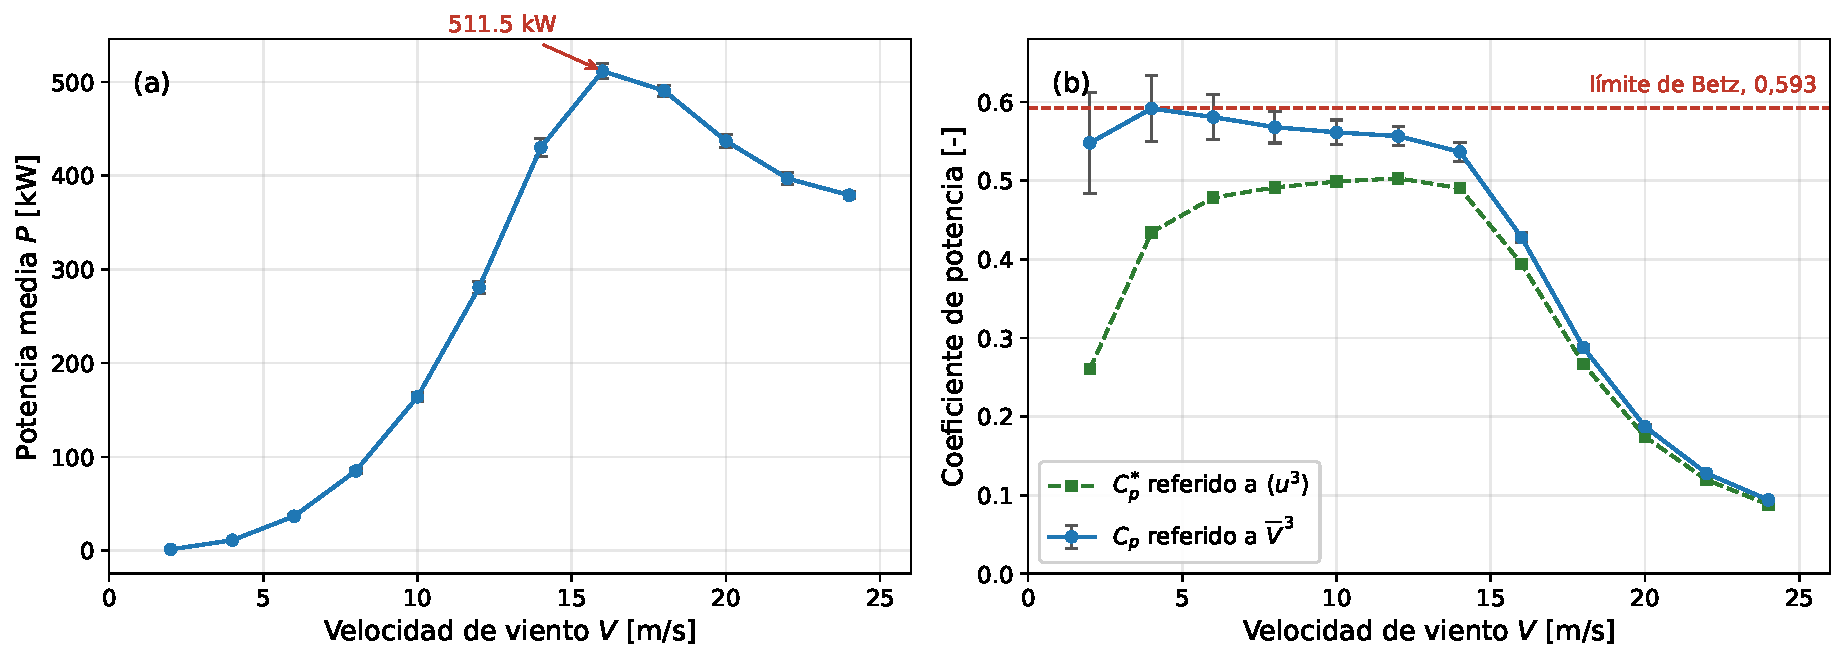
\includegraphics[width=1\textwidth]{Figuras/Figuras Resultados/curva_potencia.pdf}
    \caption{(a) Potencia media y (b) coeficiente de potencia promedio, en función de la velocidad de viento. Los puntos son el promedio de las $6$ realizaciones estocásticas simuladas por velocidad, y las barras verticales indican $\pm 1$ desviación estándar (STD) entre ellas.}
    \label{fig:curva_potencia}
\end{figure}

La barra de dispersión del primer punto de la Figura~\ref{fig:curva_potencia}b es notablemente mayor que las restantes, con una desviación estándar de $0{,}077$ en $C_p$ frente a valores entre $0{,}002$ y $0{,}020$ en el resto del rango. El origen está en la turbulencia que prescribe el NTM, ya que la desviación estándar del viento crece con la velocidad media, pero de forma menos que proporcional (Ec.~\ref{eq:ntm_sigma}), de modo que su valor relativo aumenta al bajar $V$, hasta alcanzar un $43\%$ a $2$~m/s frente a un $15\%$ a $12$~m/s. El rotor no puede seguir fluctuaciones de esa magnitud, de modo que su TSR instantáneo se dispersa con una desviación estándar de $1{,}01$ a $2$~m/s, más del triple de la que registra a $12$~m/s, y cada semilla promedia así un tramo distinto de la curva de $C_p$ frente a TSR. La dispersión no compromete las verificaciones de este capítulo, ya que la carga extrema de diseño proviene del instante registrado a $24$~m/s (Sección~\ref{sec:resultados_uls}) y el $98{,}3\%$ del daño por fatiga se concentra en las tres velocidades más altas (Sección~\ref{sec:resultados_fatiga}), de modo que la contribución de la condición de $2$~m/s a ambos estados límite es marginal.

El coeficiente de potencia de la meseta, $0{,}42$--$0{,}45$, iguala o supera el extremo superior del intervalo reportado para configuraciones H-Darrieus ($0{,}35$--$0{,}42$, Tabla~\ref{tab:tabla_vawt}) y alcanza el margen que \textcite{Essahraoui2026} atribuyen a rotores optimizados, hasta $0{,}45$. Queda así dentro de lo alcanzable por esta familia de máquinas, a diferencia del $C_{p,max} = 0{,}574$ que estima el barrido preliminar (Sección~\ref{sec:tsr_optimo}). La brecha entre ambas cifras no evidencia una inconsistencia entre métodos, sino que obedece a dos causas, una física y otra estadística. La física es la limitación del DMST ya descrita en la Sección~\ref{sec:metodos_aerodinamicos}, que las simulaciones LLFVW sí resuelven. La estadística surge de la operación bajo viento turbulento, ya que el DMST evalúa $C_{p,max}$ en un único punto estacionario, exactamente en $\lambda_{opt}$, mientras que la turbina simulada nunca permanece en ese punto.

La Figura~\ref{fig:serie_temporal_control} recorre esa segunda cadena causal para una simulación representativa a $V = 12$~m/s. La velocidad de viento incidente, panel (a), se recupera de la salida de QBlade como $V = \Omega R/\lambda$ y corresponde al campo generado por el modelo de Mann (Sección~\ref{sec:modelo_mann}); fluctúa entre $8{,}2$ y $15{,}4$~m/s en torno a una media de $11{,}7$~m/s, con una desviación estándar de $1{,}20$~m/s, un $4\%$ menor que los $1{,}25$~m/s que prescribe el NTM del emplazamiento (Sección~\ref{sec:ntm}). El panel (b) muestra que el rotor sigue esas fluctuaciones de forma suavizada, en torno a una media de $39{,}6$~rpm, ya que su inercia le impide acelerar y frenar al ritmo del viento~\parencite{Johnson2006}. El panel (c) recoge la consecuencia de ese desfase, dado que el TSR es el cociente entre ambas magnitudes y se dispersa entre $2{,}99$ y $4{,}94$ en lugar de mantenerse fijo en $\lambda_{opt}$. Para aislar el aporte del controlador, el mismo panel superpone el TSR que resultaría del mismo viento con la rotación fija en el promedio registrado ($39{,}6$~rpm). En ese escenario contrafactual la dispersión aumenta un $32\%$ (desviación estándar de $0{,}387$ frente a $0{,}292$), de modo que el controlador $K$-$\omega^2$ no solo centra el TSR en torno al óptimo, con una media de $3{,}69$ frente a $3{,}80$, sino que además reduce activamente su dispersión.

\begin{figure}[H]
    \centering
    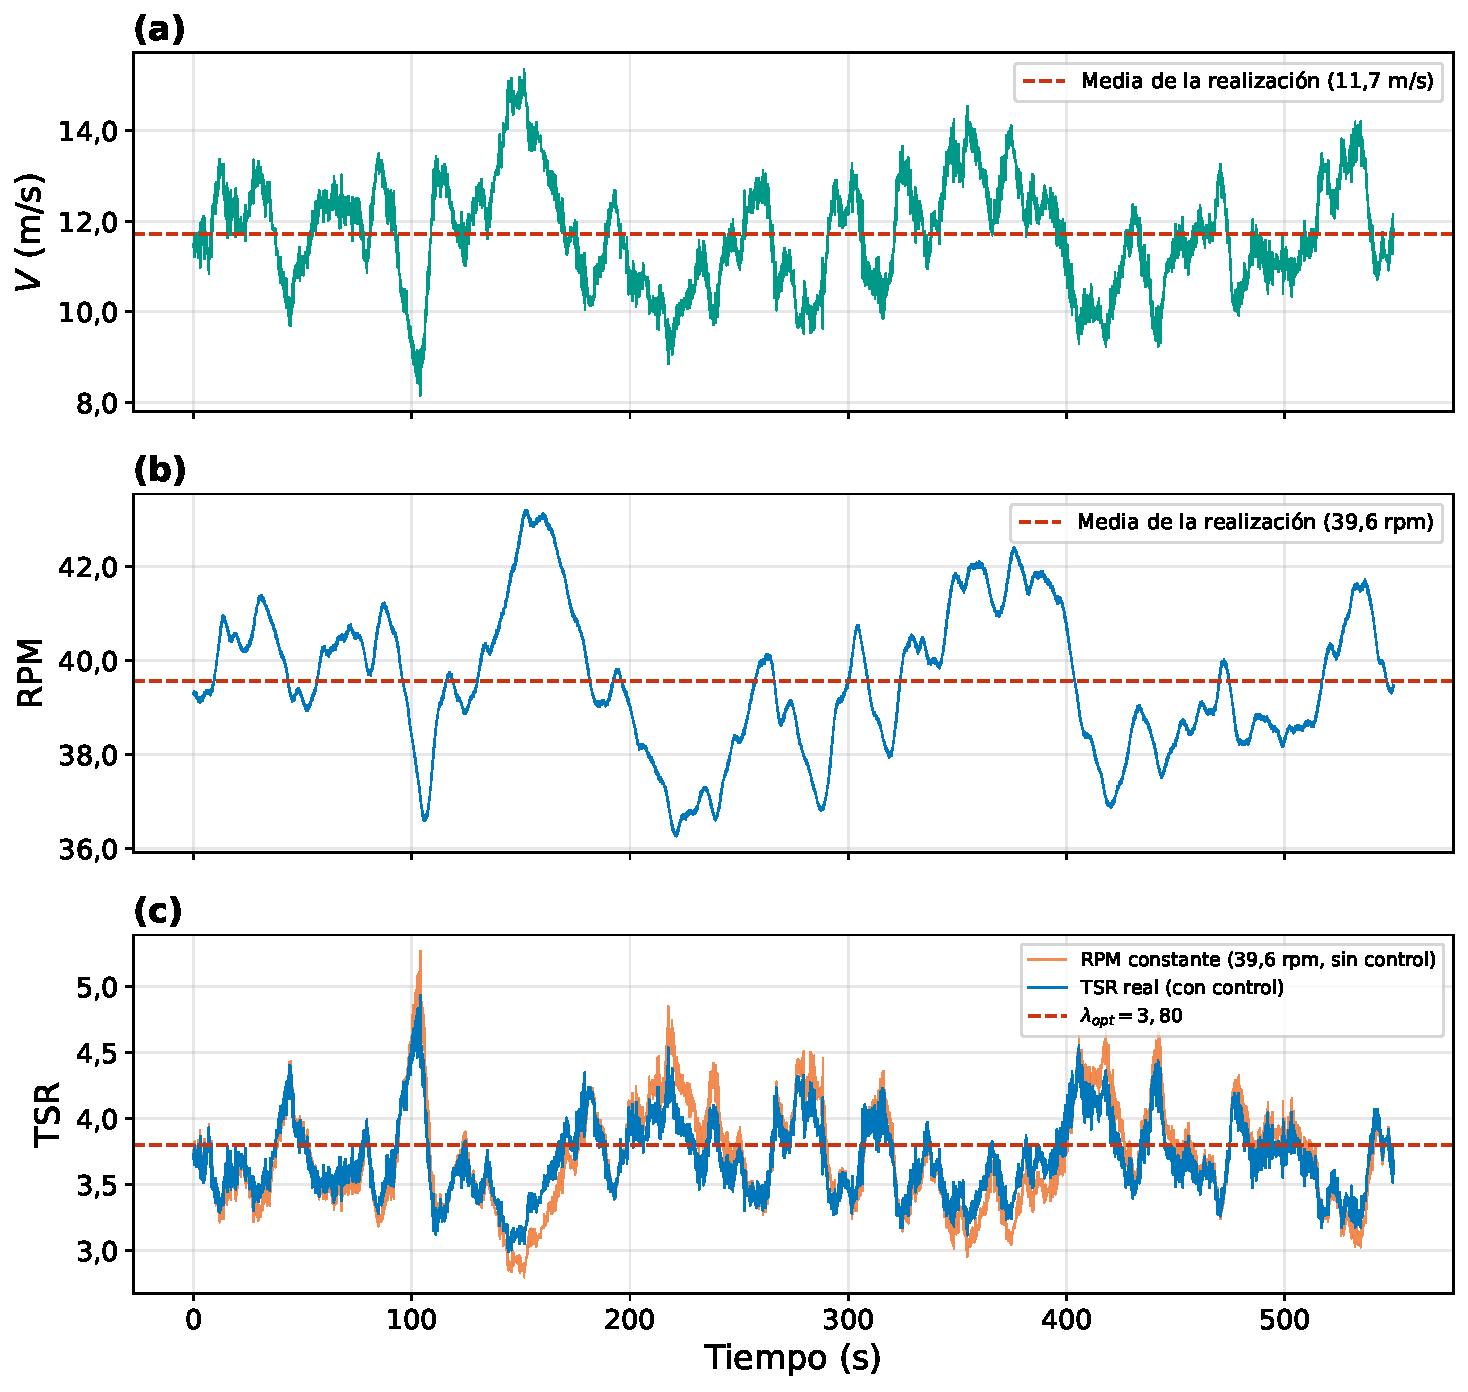
\includegraphics[width=0.95\textwidth]{Figuras/Figuras Resultados/serie_temporal_control.pdf}
    \caption[Serie temporal de viento, velocidad de rotación y TSR.]{Serie temporal de (a) velocidad de viento incidente, (b) velocidad de rotación y (c) TSR, para una simulación representativa a $V = 12$~m/s, semilla $1$. Las líneas discontinuas indican la media de la realización en (a) y (b), y $\lambda_{opt}$ en (c).}
    \label{fig:serie_temporal_control}
\end{figure}

La Tabla~\ref{tab:comparacion_adim} contrasta el rotor en estudio con las dos máquinas H-rotor de referencia de la Sección~\ref{sec:turbinas_referencia}~\parencite{Mollerstrom2019}, sobre los parámetros normalizados allí definidos. A $V = 12$~m/s la turbina del proyecto entrega $P = 201{,}5$~kW con $C_p = 0{,}432$, cifra equivalente a la potencia nominal de la T1-turbine y de la ANew-M1, ambas de $200$~kW a esa misma velocidad, y lo hace con un área de barrido intermedia entre las de ambas máquinas.

\begin{table}[H]
    \centering
    \caption[Comparación del rotor en estudio con turbinas H-rotor documentadas.]{Comparación de las dimensiones y los parámetros normalizados del rotor en estudio con turbinas H-rotor tripala documentadas y con los rangos de referencia para configuraciones H-Darrieus.}
    \label{tab:comparacion_adim}
    \begin{tabular}{lcccc}
        \hline
        \textbf{Parámetro} & \textbf{Rotor en estudio} & \textbf{T1-turbine}\textsuperscript{a} & \textbf{ANew-M1}\textsuperscript{a} & \textbf{Rango de referencia}\\
        \hline
        Diámetro $D$ (m)         & $20{,}73$ & $26{,}0$ & $24{,}0$ & ---\\
        Altura $H$ (m)           & $23{,}0$  & $24{,}0$ & $15{,}0$\textsuperscript{b} & ---\\
        Área barrida $A$ (m$^2$) & $476{,}8$ & $624$    & $360$ & ---\\
        Potencia a $12$ m/s (kW) & $201{,}5$ & $200$    & $200$ & ---\\
        $P/A$ (W/m$^2$)          & $423$     & $321$    & $556$ & $200$--$500$\textsuperscript{c}\\
        $\lambda$                & $3{,}80$  & $3{,}8$\textsuperscript{d} & --- & $2$--$5$\textsuperscript{e}\\
        $\sigma$                 & $0{,}318$ & ---      & --- & $0{,}15$--$0{,}45$\textsuperscript{e}\\
        $C_{p,max}$              & $0{,}45$  & ---      & --- & $0{,}35$--$0{,}42$\textsuperscript{e,f}\\
        \hline
        \multicolumn{5}{p{0.95\textwidth}}{\footnotesize \textsuperscript{a}Datos de \textcite{Mollerstrom2019}, Tabla~\ref{tab:hrotor_rpm}. \textsuperscript{b}Estimada como $A/D$ a partir de los datos de la fuente. \textsuperscript{c}Rango característico de un aerogenerador moderno~\parencite{Mollerstrom2019}. \textsuperscript{d}TSR objetivo documentado para la T1-turbine (Tabla~\ref{tab:t1_params})~\parencite{Mollerstrom2017,Mollerstrom2016}. \textsuperscript{e}Rango reportado para configuraciones H-Darrieus~\parencite{Essahraoui2026}, Tabla~\ref{tab:tabla_vawt}. \textsuperscript{f}La misma fuente reporta hasta $0{,}45$ para rotores optimizados.}
    \end{tabular}
\end{table}

La potencia específica del rotor en estudio se sitúa entre la de la T1-turbine y la de la ANew-M1, dentro del rango propio de un aerogenerador moderno~\parencite{Mollerstrom2019}, y su $\lambda_{opt} = 3{,}80$ coincide con el \gls{tsr} objetivo documentado para la T1-turbine~\parencite{Mollerstrom2017}. La solidez y el coeficiente de potencia caen igualmente dentro de sus rangos de referencia~\parencite{Essahraoui2026}. El dimensionamiento y el punto de operación del rotor resultan, por tanto, consistentes con los de las máquinas construidas de esta familia y escala.

El pico de $P_{max} = 503{,}4$~kW a $V = 18$~m/s corresponde a $1056$~W/m$^2$. Esta cifra no describe el dimensionamiento nominal de la máquina, sino la capacidad de sobrecarga instantánea del rotor operando fuera de su punto de diseño, y resulta del orden de los valores máximos reportados históricamente para VAWT~\parencite{Mollerstrom2019}.

La caída del coeficiente de potencia para $V > 16$~m/s es consecuencia directa de la estrategia de control, ya que al alcanzar el límite de velocidad de rotación de $42$~rpm el TSR decrece de $3{,}7$ a $1{,}8$, alejándose del $\lambda_{opt} = 3{,}80$. La pérdida es deliberada, ya que sostener el TSR óptimo a $24$~m/s exigiría girar a $84$~rpm, el doble del límite adoptado, con lo que las cargas centrífugas, proporcionales a $\Omega^2$, se cuadruplicarían. Dado que las velocidades superiores a $20$~m/s representan solo el $0{,}48\%$ de las horas del año en el emplazamiento, esto es, $42$~h/año (Sección~\ref{sec:recurso_eolico}), el costo energético de esa decisión es marginal frente al alivio estructural que proporciona.

\section{Cargas aerodinámicas para DLC 1.1}
\label{sec:resultados_uls}

Las series temporales de fuerzas obtenidas de las simulaciones anteriores constituyen la base de las verificaciones normativas que siguen. Para el DLC 1.1, los seis valores de $F_{max}$ por velocidad, el máximo de la fuerza total integrada $F_{tot}(t)$ en cada simulación (Sección~\ref{sec:anexo_f}), se ajustan a una distribución de Gumbel~\parencite{Gumbel1958}; la Tabla~\ref{tab:cargas_extremas} presenta los parámetros resultantes, junto con $F_{obs,max}$, el mayor de esos seis valores observados a cada velocidad.

\begin{table}[H]
    \centering
    \caption{Parámetros del ajuste de Gumbel para $F_{tot}$ por velocidad de viento ($N = 6$ semillas).}
    \label{tab:cargas_extremas}
    \begin{tabular}{lccc}
        \hline
        $V$ (m/s) & $\mu_j$ (kN) & $\beta_j$ (kN) & $F_{obs,max}$ (kN) \\
        \hline
        $2$  & $1{,}460$  & $0{,}15$  & $1{,}760$ \\
        $4$  & $6{,}190$  & $0{,}96$  & $9{,}230$ \\
        $6$  & $11{,}43$ & $0{,}90$  & $14{,}05$ \\
        $8$  & $19{,}66$ & $0{,}78$  & $21{,}60$ \\
        $10$ & $31{,}50$ & $1{,}36$  & $34{,}61$ \\
        $12$ & $42{,}42$ & $1{,}99$  & $47{,}06$ \\
        $14$ & $53{,}34$ & $0{,}97$  & $55{,}29$ \\
        $16$ & $63{,}10$ & $1{,}36$  & $66{,}66$ \\
        $18$ & $73{,}42$ & $1{,}91$  & $78{,}17$ \\
        $20$ & $84{,}70$ & $0{,}85$  & $86{,}04$ \\
        $22$ & $88{,}20$ & $1{,}26$  & $90{,}81$ \\
        $24$ & $100{,}8$ & $2{,}44$ & $106{,}8$ \\
        \hline
    \end{tabular}
\end{table}

Los parámetros $\mu_j$ y $\beta_j$ corresponden a la localización y escala de la distribución de Gumbel~\parencite{Gumbel1958}, estimados por el método de los momentos sobre los seis máximos observados a cada velocidad (Sección~\ref{sec:anexo_f}). Tanto $\mu_j$ como $F_{obs,max}$ crecen monótonamente con $V$, en línea con la dependencia $F \propto V^2$ de las fuerzas aerodinámicas. La Figura~\ref{fig:cargas_maximas} muestra la dispersión de estos máximos por velocidad junto con los percentiles $50\%$, $90\%$ y $99\%$ de las distribuciones ajustadas.

\begin{figure}[H]
    \centering
    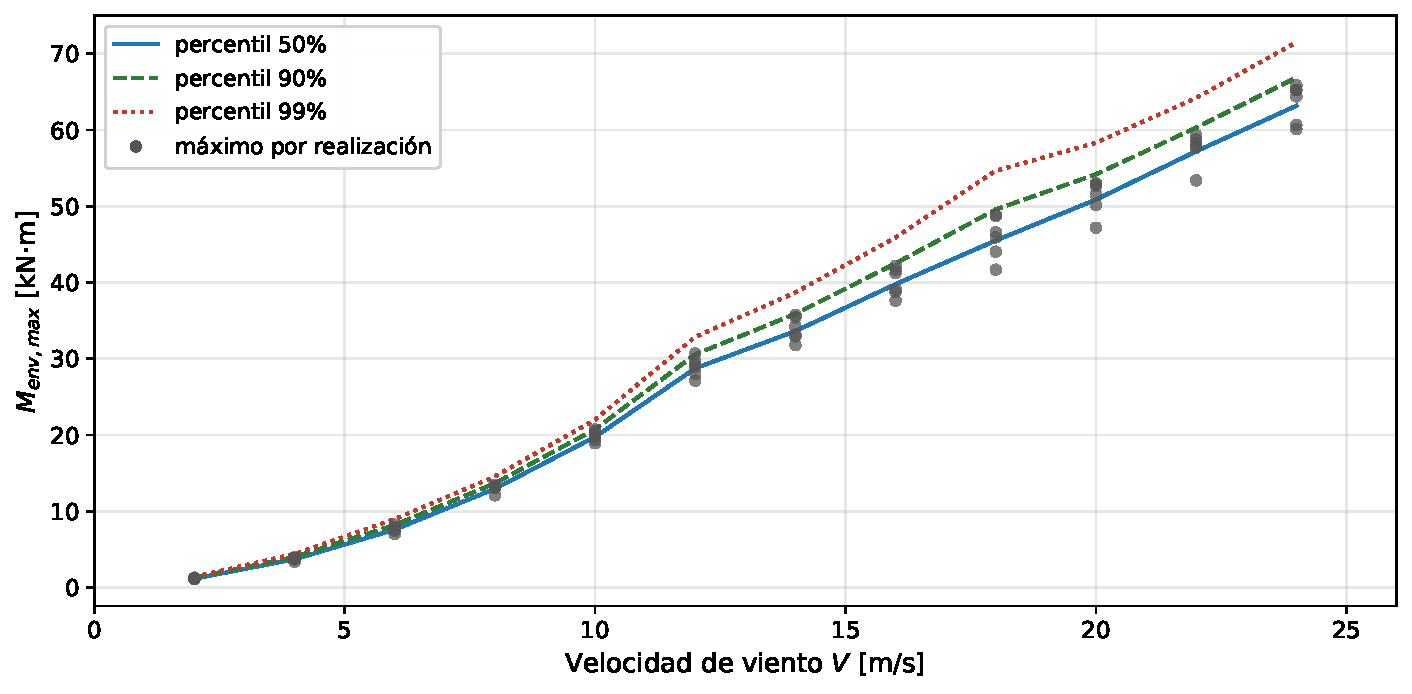
\includegraphics[width=0.9\textwidth]{Figuras/Figuras Resultados/cargas_maximas_global.pdf}
    \caption{Fuerza total máxima integrada por simulación y percentiles de Gumbel por velocidad de viento.}
    \label{fig:cargas_maximas}
\end{figure}
La dispersión de puntos para una misma velocidad refleja que, aunque las seis simulaciones comparten la misma velocidad media y la misma intensidad de turbulencia objetivo, cada una corresponde a una semilla distinta del campo de viento de Mann (Sección~\ref{sec:modelo_mann}), es decir, a una secuencia distinta de ráfagas; el $F_{max}$ que arroja cada simulación depende de la ráfaga más severa efectivamente contenida en esa realización particular, no solo de los parámetros estadísticos que todas comparten.

Esa dispersión se ensancha con la velocidad de viento, en línea con el parámetro de escala $\beta_j$ de la Tabla~\ref{tab:cargas_extremas}, que pasa de $0{,}15$~kN a $2$~m/s a $2{,}44$~kN a $24$~m/s. Como la separación entre percentiles de una distribución de Gumbel es proporcional a $\beta_j$~\parencite{Gumbel1958}, la distancia entre los percentiles $50\%$ y $99\%$ crece de $0{,}6$ a $10{,}3$~kN entre ambos extremos del rango. El crecimiento responde a dos efectos que actúan en el mismo sentido, ya que las fuerzas aerodinámicas dependen del cuadrado de la velocidad relativa (Ecs.~\ref{eq:fuerza_sustentacion} y~\ref{eq:fuerza_arrastre}) y la desviación estándar absoluta del viento que prescribe el NTM también aumenta con $V$ (Ec.~\ref{eq:ntm_sigma})~\parencite{IEC61400-1}. En términos relativos, en cambio, la dispersión se estrecha, ya que esa separación equivale al $44\%$ de $\mu_j$ a $2$~m/s y solo al $10\%$ a $24$~m/s.

El crecimiento de $\beta_j$ no es monótono, sino que oscila entre velocidades contiguas. Ello es esperable, dado que cada $\beta_j$ se estima sobre solo seis observaciones. Un remuestreo de la propia distribución ajustada, con $2 \times 10^5$ muestras de tamaño seis, sitúa el error estándar relativo del estimador por momentos de $\beta$ en un $41\%$, con el $90\%$ de las estimaciones comprendido entre $0{,}42$ y $1{,}62$ veces el valor real. La oscilación observada es, por tanto, del orden de la incertidumbre que impone el tamaño de muestra y no revela una deficiencia del ajuste. Aun así, las curvas de percentiles muestran que el modelo de Gumbel envuelve adecuadamente las observaciones, ya que las $72$ quedan por debajo del percentil $99\%$ de su velocidad. La calidad del ajuste se examina con mayor detalle en la Figura~\ref{fig:gumbel_pp}, que presenta el papel de probabilidad de Gumbel para cuatro velocidades representativas.

\begin{figure}[H]
    \centering
    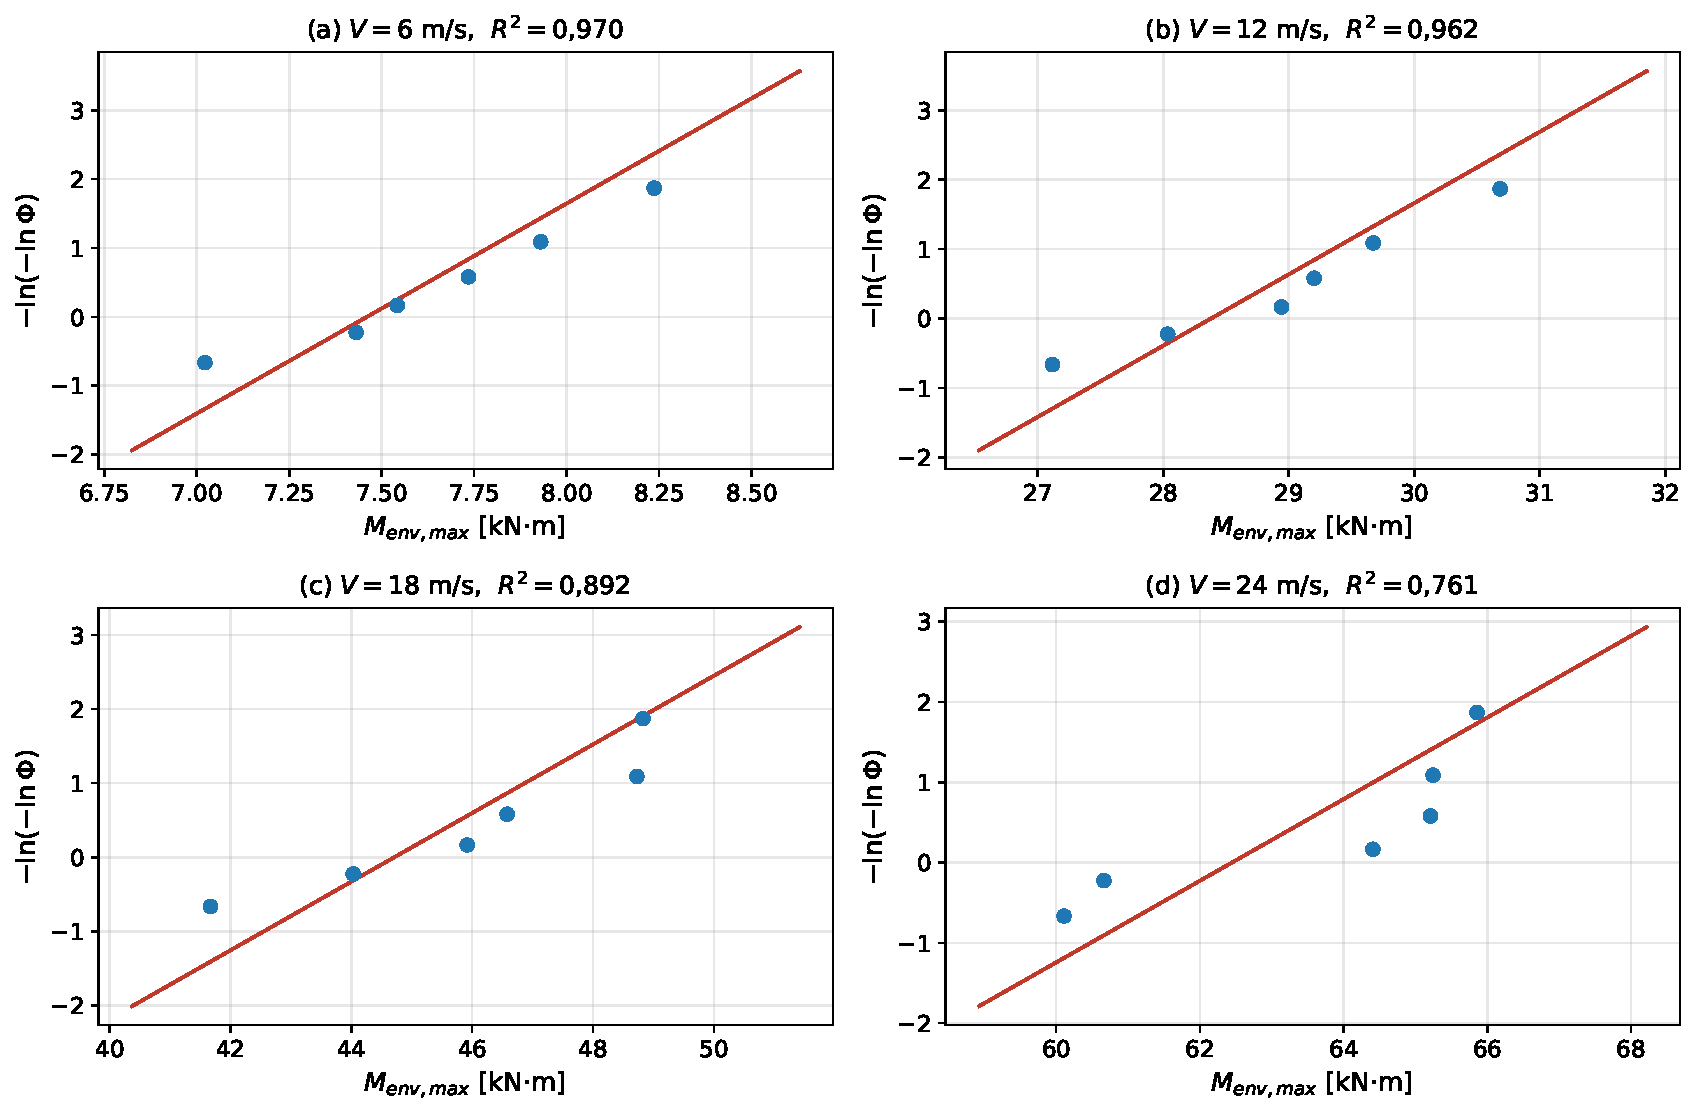
\includegraphics[width=1\textwidth]{Figuras/Figuras Resultados/gumbel_probability_paper.pdf}
    \caption{Papel de probabilidad de Gumbel para cuatro velocidades representativas. El $R^2$ de cada panel mide la linealidad de los puntos empíricos.}
    \label{fig:gumbel_pp}
\end{figure}


El papel de probabilidad es una representación en la que la distribución ajustada se convierte en una recta, de modo que la calidad del ajuste puede evaluarse a simple vista~\parencite{Gumbel1958}. Se construye aplicando a la función de distribución acumulada de Gumbel (Ec.~\ref{eq:gumbel_anexof}) la transformación $-\ln(-\ln(\Phi))$, que la reduce a $(F - \mu_j)/\beta_j$, una función lineal de la carga. El eje vertical de cada panel es esa variable reducida, y a cada uno de los seis máximos ordenados de menor a mayor se le asigna una probabilidad empírica de no excedencia $i/(n+1)$, con $i$ el orden del dato y $n = 6$. Si la distribución describe correctamente los datos, los puntos así construidos deben alinearse sobre la recta de pendiente $1/\beta_j$ que define el ajuste.

Las cuatro velocidades representativas, que cubren el rango bajo ($V = 6$~m/s), medio ($12$~m/s), alto ($18$~m/s) y extremo ($24$~m/s) del espectro operacional, presentan coeficientes de determinación $R^2$ entre $0{,}833$ y $0{,}963$, valores razonables para ajustes sobre solo seis observaciones, lo que respalda el uso de la distribución de Gumbel para modelar los máximos de $F_{tot}$.

En la Figura \ref{fig:gumbel_pp}d, se ve que tres de sus seis puntos se alinean verticalmente y se apartan de la recta. No se trata de un defecto del ajuste, sino de que esas tres semillas arrojan máximos prácticamente idénticos, comprendidos entre $100{,}459$ y $100{,}462$~kN, con una diferencia máxima de $3$~N que equivale al $0{,}003\%$ de la carga. Al compartir abscisa y diferir solo en su posición de graficado, esos tres puntos quedan forzosamente sobre una vertical, que ninguna recta puede seguir. La coincidencia proviene del régimen de operación, ya que a $24$~m/s el rotor gira en su límite de velocidad y la variación de la carga a lo largo de la revolución, idéntica en todas las semillas por depender solo de la rotación, domina sobre la contribución turbulenta que las diferencia. De ahí que el recorrido relativo de los máximos se reduzca del $29\%$ de la media a $6$~m/s a un $7\%$ a $24$~m/s, pese a que en términos absolutos la dispersión crece.

La carga característica $F_k$, correspondiente al período de retorno de $50$ años, y la carga de diseño $F_d$, que resulta de mayorarla por el factor parcial, se obtienen a partir de esta distribución mediante el procedimiento de bisección descrito en la Sección~\ref{sec:anexo_f}.

La probabilidad de excedencia objetivo de la Ec.~\ref{eq:fk_criterion}, con $T_{obs} = 600$~s y $T_{retorno} = 50$ años, resulta:

\begin{equation}
    P_e(F_k) = \frac{600\ \text{s}}{50 \times 365{,}25 \times 24 \times 3600\ \text{s}} = 3{,}8 \times 10^{-7}
    \label{eq:fk_criterion_num}
\end{equation}

La carga característica global para un período de retorno de 50 años, esto es, el valor de $F_{max}$ que satisface la Ec.~\ref{eq:fk_criterion_num}, es $F_{tot,k} = 116{,}9$~kN. La carga de diseño para el DLC 1.1 según el Anexo F de IEC 61400-1~\parencite{IEC61400-1} se obtiene aplicando el factor de seguridad parcial $\gamma_f = 1{,}25$, según la Ec.~\ref{eq:Fd_dlc11_res}:

\begin{equation}
F_{tot,d} = \gamma_f \cdot F_{tot,k} = 1{,}25 \times 116{,}9 = 146{,}1\ \text{kN}
\label{eq:Fd_dlc11_res}
\end{equation}

El instante de máxima solicitación global entre las 72 simulaciones ocurre a $V = 24$~m/s (semilla 4, $t = 188{,}3$~s), con $F_{tot} = 106{,}8$~kN; las fuerzas compañeras de ese instante se escalan por el factor $146{,}1/106{,}8 = 1{,}368$ para construir el perfil de diseño.

La distribución de esta carga a lo largo de la envergadura, esto es, las fuerzas de diseño por estación $F_{d,x}[p]$ y $F_{d,y}[p]$ para las 24 estaciones de la pala, se presenta en la Sección~\ref{sec:comparacion_dlc}, junto con la del DLC 1.3, una vez determinada la carga de este último.

\section{Cargas aerodinámicas para DLC 1.3}
\label{sec:resultados_dlc13}

Las 30 simulaciones correspondientes al DLC 1.3 (ETM, $V = 16$ a $24$~m/s) se procesan según el método de la media de máximos prescrito en la Sección 7.6.2 de la norma IEC 61400-1~\parencite{IEC61400-1}. La Tabla~\ref{tab:dlc13_maximos} presenta los máximos observados para cada una de las 6 semillas y la media por velocidad, calculados con la misma definición de $F_{tot}$ de la Ec.~\ref{eq:F_tot}.

\begin{table}[H]
    \centering
    \caption{Máximos de fuerza total integrada $F_{tot}$ por velocidad y semilla para DLC 1.3 (ETM).}
    \label{tab:dlc13_maximos}
    \begin{tabular}{lccccccc}
        \hline
        & \multicolumn{7}{c}{$F_{tot,max}$ (kN)} \\
        \cline{2-8}
        $V$ (m/s) & $S_1$ & $S_2$ & $S_3$ & $S_4$ & $S_5$ & $S_6$ & Media \\
        \hline
        $16$ & $70{,}7$ & $78{,}7$ & $69{,}9$ & $70{,}4$ & $69{,}5$ & $81{,}0$ & $73{,}4$ \\
        $18$ & $87{,}5$ & $84{,}4$ & $82{,}7$ & $77{,}6$ & $80{,}4$ & $88{,}6$ & $83{,}6$ \\
        $20$ & $88{,}8$ & $97{,}8$ & $88{,}7$ & $89{,}3$ & $91{,}1$ & $88{,}9$ & $90{,}8$ \\
        $22$ & $101{,}9$ & $101{,}8$ & $102{,}1$ & $106{,}4$ & $106{,}0$ & $102{,}0$ & $103{,}4$ \\
        $24$ & $107{,}7$ & $113{,}8$ & $113{,}0$ & $119{,}5$ & $108{,}7$ & $113{,}2$ & $\mathbf{112{,}6}$ \\
        \hline
    \end{tabular}
\end{table}

La carga característica corresponde a la mayor media entre las velocidades simuladas, $F_k = 112{,}6$~kN a $V = 24$~m/s (Destacada en la Tabla \ref{tab:dlc13_maximos}). Aplicando $\gamma_f = 1{,}35$ (Tabla 3 de la norma IEC 61400-1~\parencite{IEC61400-1}, situaciones normales sin extrapolación estadística), la carga de diseño resulta según la Ec.~\ref{eq:Fd_dlc13_res}:

\begin{equation}
    F_{d,\text{DLC 1.3}} = \gamma_f \cdot F_k = 1{,}35 \times 112{,}6 = 152{,}1\ \text{kN}
    \label{eq:Fd_dlc13_res}
\end{equation}

La Sección 7.4.1 de la norma IEC 61400-1~\parencite{IEC61400-1} vincula explícitamente ambos casos de carga, ya que permite omitir el análisis del DLC 1.1 cuando los valores extremos de diseño obtenidos del DLC 1.3 lo superan y prescribe, en caso contrario, aumentar la constante $c_{ETM}$ del modelo de turbulencia extrema hasta que el DLC 1.3 lo envuelva. Esa constante, cuyo valor por defecto de $2$~m/s fija la Sección 6.3.2.3 de la norma IEC 61400-1~\parencite{IEC61400-1}, es la adoptada en las simulaciones de este trabajo (Sección~\ref{sec:velocidades_simulacion}), sin recurrir al aumento que la norma habilita. El ETM del DLC 1.3 existe, por tanto, para sustituir la extrapolación estadística del DLC 1.1~\parencite{Galinos2015}.

Las cargas características sitúan al DLC 1.1 por encima, con $116{,}9$~kN por extrapolación estadística del NTM frente a $112{,}6$~kN por media de máximos del ETM, una diferencia del $3{,}7\%$. El orden se invierte en las cargas de diseño, $146{,}1$~kN y $152{,}1$~kN respectivamente, pero esa inversión la producen los factores parciales y no las cargas, ya que la Tabla 3 de la norma IEC 61400-1~\parencite{IEC61400-1} admite $\gamma_f = 1{,}25$ para el DLC 1.1 por determinarse mediante extrapolación estadística, frente al $\gamma_f = 1{,}35$ del DLC 1.3.

\textcite{Galinos2015} obtiene el mismo ordenamiento de las cargas características en un rotor Darrieus de $5$~MW, donde los valores extrapolados del DLC 1.1 superan a los del DLC 1.3 incluso al elevar $c_{ETM}$ a $3$~m/s. La explicación que propone es que las cargas de una VAWT están dominadas por la fluctuación determinista a frecuencia $1P$, esto es, la que se repite una vez por cada revolución del rotor, ya que cada pala recorre en cada vuelta un ciclo completo de ángulo de ataque (Sección~\ref{sec:aerodinamica}). Esa componente no depende de la turbulencia, por lo que las cargas de una VAWT resultan menos sensibles a ella que las de una HAWT, de modo que el ETM, que actúa amplificando precisamente la componente turbulenta, eleva la carga de una VAWT menos de lo que la elevaría en la máquina de eje horizontal sobre la que fue calibrado. Esa dominancia determinista se observa igualmente en las simulaciones de este trabajo, ya que a $24$~m/s tres de las seis semillas del DLC 1.1 arrojan máximos que coinciden dentro del $0{,}003\%$ (Sección~\ref{sec:resultados_uls}). El propio autor advierte, no obstante, que su conclusión proviene del análisis de un único rotor Darrieus y que debe verificarse sobre otros modelos antes de proponer cambios a la norma.

El criterio que la Sección 7.4.1 de la norma IEC 61400-1~\parencite{IEC61400-1} define para esa omisión se evalúa sobre los momentos flectores en la raíz de la pala y la deflexión de punta, no sobre la carga global. Como se verá en la Sección~\ref{sec:resultados_fem}, los resultados del modelo estructural muestran que el DLC 1.3 no supera al DLC 1.1 en ninguna de las dos magnitudes con que aquí se verifica la pala, con una deflexión de $0{,}164$~m frente a $0{,}169$~m y una tensión principal máxima de $156{,}8$~MPa frente a $163{,}4$~MPa. El análisis del DLC 1.1 no puede omitirse y ambos casos se conservan en la verificación.

Que el DLC 1.1 gobierne pese a su menor carga de diseño responde a la forma de los perfiles de carga. El del DLC 1.1 proviene de un único instante de la simulación y concentra la solicitación en el vano central, mientras que el del DLC 1.3, construido como media de máximos por estación, resulta espacialmente más suave (Sección~\ref{sec:comparacion_dlc}).

\section{Comparación de fuerzas por estación entre DLC}
\label{sec:comparacion_dlc}

Definidas las cargas globales de ambos casos últimos, resta distribuirlas a lo largo de la pala para su aplicación en el modelo estructural. La Figura~\ref{fig:comparacion_fuerzas_dlc} presenta el perfil de fuerzas de diseño $F_d$ a lo largo de la envergadura para ambos casos, construido en cada uno según el procedimiento que le corresponde, con escalamiento uniforme de las fuerzas compañeras del instante de máxima solicitación global en el DLC 1.1 (Sección~\ref{sec:anexo_f}), y media por estación de los perfiles de las seis semillas a la velocidad gobernante en el DLC 1.3 (Sección~\ref{sec:anexo_dlc13}).

\begin{figure}[H]
    \centering
    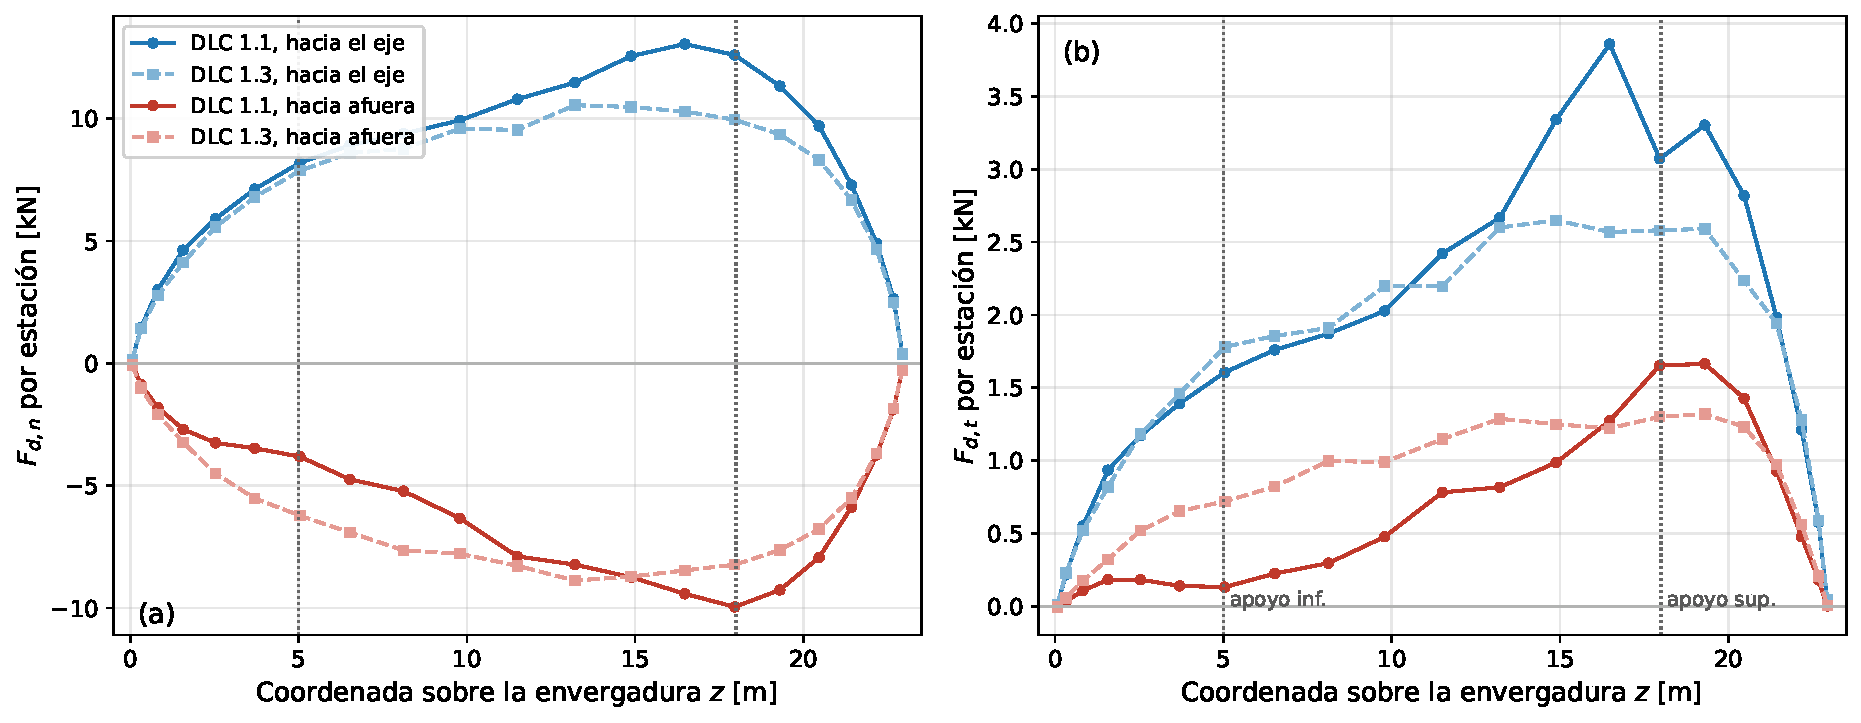
\includegraphics[width=1\textwidth]{Figuras/Figuras Resultados/comparacion_fuerzas_dlc.pdf}
    \caption{Comparación de fuerzas de diseño por estación entre DLC 1.1 (NTM) y DLC 1.3 (ETM): (a) componente normal a la cuerda $F_{d,x}$ y (b) componente en el sentido de la cuerda $F_{d,y}$, según los ejes locales de la Figura~\ref{fig:ejes_locales}. El eje vertical del panel (b) está invertido, ya que $F_{d,y}$ es negativa en todas las estaciones.}
    \label{fig:comparacion_fuerzas_dlc}
\end{figure}

Cada panel de la Figura~\ref{fig:comparacion_fuerzas_dlc} recorre la envergadura desde la raíz ($z = 0$) hasta la punta ($z = 23$~m) y compara, estación por estación, la fuerza de diseño de ambos casos en una de las dos direcciones del sistema local de la pala (Figura~\ref{fig:ejes_locales}). El panel (a) corresponde a la componente normal a la cuerda, $F_{d,x}$, y el (b) a la componente en el sentido de la cuerda, $F_{d,y}$. Las líneas verticales punteadas marcan las dos conexiones con los brazos, en $z = 5$ y $z = 17$~m, que separan los dos tramos en voladizo del vano central.

Ambos paneles conservan el signo de la fuerza. En el instante de diseño, $F_{d,x}$ es positiva y $F_{d,y}$ negativa en las 24 estaciones de los dos casos, lo que significa que la componente normal apunta hacia el extradós y la tangencial hacia el borde de ataque, según la orientación de los ejes $X_l$ e $Y_l$ de la Figura~\ref{fig:ejes_locales}. El eje vertical del panel (b) se representa invertido para que, mostrando los valores negativos que corresponden, la curva no quede dibujada hacia abajo. La componente normal domina el estado de carga, ya que su cociente con la tangencial, $|F_{d,x}/F_{d,y}|$, se mantiene entre $2{,}8$ y $3{,}0$ a lo largo de todo el vano central en ambos casos, y solo crece en las dos estaciones extremas, donde ambas componentes son pequeñas y su cociente pierde significado. Ese predominio es el esperable en un perfil con flujo adherido, donde la sustentación, perpendicular a la cuerda, supera con holgura a la fuerza en el sentido de la cuerda.

Las dos distribuciones concentran la carga en la región media de la pala y decaen hacia la raíz y la punta, pero difieren en la forma de ese decaimiento. El perfil del DLC 1.1 tiene un máximo definido en $z \approx 10$--$11$~m y desde ahí disminuye de forma progresiva, mientras que el del DLC 1.3 se mantiene casi plano a lo largo del vano central y de los tramos contiguos. En la componente tangencial, entre $z = 5$ y $z = 18$~m el perfil del DLC 1.3 varía un $3\%$ frente al $19\%$ del DLC 1.1, y entre su máximo y $z = 20$~m el DLC 1.1 pierde un $27\%$ frente al $6\%$ del DLC 1.3. La caída abrupta del DLC 1.3 se concentra en la última estación, donde pierde un $79\%$. La diferencia proviene de cómo se construye cada perfil. El del DLC 1.1 es un único instante de una única realización, de modo que conserva la distribución espacial que la simulación entrega en ese momento, con su máximo en una posición concreta. El del DLC 1.3 promedia estación por estación los perfiles compañeros de las seis semillas, cada uno tomado en el instante de máxima solicitación de su propia realización (Sección~\ref{sec:anexo_dlc13}); como esos seis instantes corresponden a azimuts y campos de viento distintos, el promedio atenúa los rasgos propios de cada uno y entrega una distribución más uniforme. El resultado es que las fuerzas del DLC 1.3 superan a las del DLC 1.1 en los tramos en voladizo, mientras que en el vano central entre brazos ambas componentes del DLC 1.1 resultan mayores, diferencia que tiene consecuencias directas sobre la respuesta estructural, como se verá en la Sección~\ref{sec:resultados_fem}.

La caída de la carga hacia los dos extremos responde a las pérdidas de punta, ya que los vórtices desprendidos en los extremos libres de la pala inducen velocidades que reducen el ángulo de ataque efectivo, y con ello la sustentación, en esas regiones~\parencite{Anderson2016}, efecto que el método LLFVW resuelve implícitamente (Sección~\ref{sec:metodos_aerodinamicos})~\parencite{marten2019qblade}.

La tabla completa de fuerzas $F_{d,x}$ y $F_{d,y}$ para las 24 estaciones, expresadas como resultantes por segmento, se presenta en el \hyperref[anexo:fuerzas]{Anexo~A} para su ingreso directo al modelo de elementos finitos en Ansys, construida según los procedimientos de las Secciones~\ref{sec:anexo_f} y~\ref{sec:anexo_dlc13}.

\section{Evaluación de fatiga (DLC 1.2)}
\label{sec:resultados_fatiga}

La verificación a fatiga del DLC 1.2 se presenta siguiendo la cadena de cálculo: el procesamiento de las series de carga en ciclos de tensión y su escalamiento a un año de operación; el contraste de la demanda así obtenida con la curva S-N del material; la distribución del daño anual entre las velocidades del rango operacional; y el daño acumulado sobre la vida útil de diseño.

\subsection{Procesamiento de las series de carga}

Las 72 series temporales del DLC 1.2 se procesan mediante el momento flector $M_{res}(t)$ en la sección crítica $z_{crit} = 5$~m (conexión con el brazo inferior, donde el FEM localiza la tensión máxima) y el factor de proporcionalidad $K_{aero} = 0{,}752$~MPa/(kN$\cdot$m), conforme a la metodología descrita en la Sección~\ref{sec:anexo_g}. Dicho factor resulta de las dos corridas FEM de la Sección~\ref{sec:resultados_fem}, como la tensión bajo la carga de diseño completa, $\sigma_{1,\max} = 163{,}4$~MPa, menos la que producen las cargas inerciales por sí solas, $\sigma_{in} = 114{,}5$~MPa, dividida por el momento de diseño de $65{,}0$~kN$\cdot$m. Esta última tensión se reincorpora después como el nivel medio sobre el que oscila la historia de tensión. Sobre esa historia se aplica el conteo de ciclos Rainflow~\parencite{ASTM_E1049,Matsuishi1968} y la corrección por tensión media según el diagrama de Goodman, conforme exige la Sección 7.6.3 de la norma IEC 61400-1~\parencite{IEC61400-1}. Dado que cada simulación cubre únicamente $T_{sim} = 550$~s, los ciclos contabilizados a cada velocidad deben expandirse al tiempo que el viento permanece en ese intervalo a lo largo de un año. La Tabla~\ref{tab:weibull_fatiga} presenta los parámetros de dicho escalamiento temporal para las doce velocidades del rango operacional. Una serie temporal representativa del procesamiento Rainflow para $V = 10$~m/s se presenta en el \hyperref[anexo:fuerzas]{Anexo~A}.

En la Tabla~\ref{tab:weibull_fatiga}, $f_W(V)$ es la densidad de probabilidad de Weibull, $t_j$ el tiempo anual que el viento permanece en cada intervalo de velocidad y $t_j/T_{sim}$ el número de simulaciones equivalentes por año.

\begin{table}[H]
    \centering
    \caption{Parámetros de escalamiento temporal según la distribución de Weibull del emplazamiento.}
    \label{tab:weibull_fatiga}
    \begin{tabular}{lccccc}
        \hline
        $V$ (m/s) & $f_W(V)$ & Prob. (\%) & $t_j$ (h/año) & $t_j$ (s/año) & $t_j/T_{sim}$ \\
        \hline
        $2$  & $0{,}0431$ & $8{,}62$ & $761{,}9$  & $2{,}74 \times 10^6$ & $4\,986$ \\
        $4$  & $0{,}0794$ & $15{,}89$ & $1\,407{,}9$ & $5{,}07 \times 10^6$ & $9\,216$ \\
        $6$  & $0{,}0967$ & $19{,}34$ & $1\,711{,}7$ & $6{,}16 \times 10^6$ & $11\,204$ \\
        $8$  & $0{,}0930$ & $18{,}59$ & $1\,641{,}0$ & $5{,}91 \times 10^6$ & $10\,741$ \\
        $10$ & $0{,}0746$ & $14{,}91$ & $1\,310{,}9$ & $4{,}72 \times 10^6$ & $8\,581$ \\
        $12$ & $0{,}0511$ & $10{,}22$ & $893{,}5$  & $3{,}22 \times 10^6$ & $5\,848$ \\
        $14$ & $0{,}0303$ & $6{,}05$  & $525{,}7$  & $1{,}89 \times 10^6$ & $3\,441$ \\
        $16$ & $0{,}0156$ & $3{,}12$  & $268{,}8$  & $9{,}68 \times 10^5$ & $1\,760$ \\
        $18$ & $0{,}0070$ & $1{,}40$  & $119{,}9$  & $4{,}32 \times 10^5$ & $785$ \\
        $20$ & $0{,}0027$ & $0{,}55$  & $46{,}8$   & $1{,}68 \times 10^5$ & $306$ \\
        $22$ & $0{,}0009$ & $0{,}19$  & $16{,}0$   & $5{,}76 \times 10^4$ & $105$ \\
        $24$ & $0{,}0003$ & $0{,}06$  & $4{,}8$    & $1{,}72 \times 10^4$ & $31$ \\
        \hline
    \end{tabular}
\end{table}

El factor $t_j/T_{sim}$ cuantifica cuántas veces debe repetirse el espectro de ciclos de cada simulación para representar un año de operación. Su distribución sigue directamente a la de Weibull del emplazamiento, ya que alcanza su máximo en las velocidades intermedias ($V = 6$--$8$~m/s), las más frecuentes, y cae más de dos órdenes de magnitud hacia el extremo superior del rango, donde el viento sopla solo unas pocas horas al año. Aplicado este escalamiento, el espectro de ciclos de cada simulación queda expresado sobre un año de operación y puede contrastarse con la resistencia del material.

\subsection{Curva S-N y espectro de fatiga}

La Figura~\ref{fig:curva_sn_gfrp} presenta la curva S-N del GFRP en sus formas nominal y factoreada ($\gamma_m = 1{,}7$, $\gamma_n = 1{,}15$ según la Sección 7.6.3 de la norma IEC 61400-1~\parencite{IEC61400-1}), junto con el espectro colectivo anual que resulta del escalamiento anterior. En la ecuación de Basquin~\parencite{Basquin1910}, la resistencia última $\sigma_u = 242{,}1$~MPa corresponde al valor proporcionado por el fabricante de la pala (Tabla~\ref{tab:material_pala}), mientras que el exponente de fatiga $b = -0{,}045$ proviene de \textcite{Huh2012} para un tejido bidireccional ($\pm 45^\circ$) fabricado por infusión al vacío.

\begin{figure}[H]
    \centering
    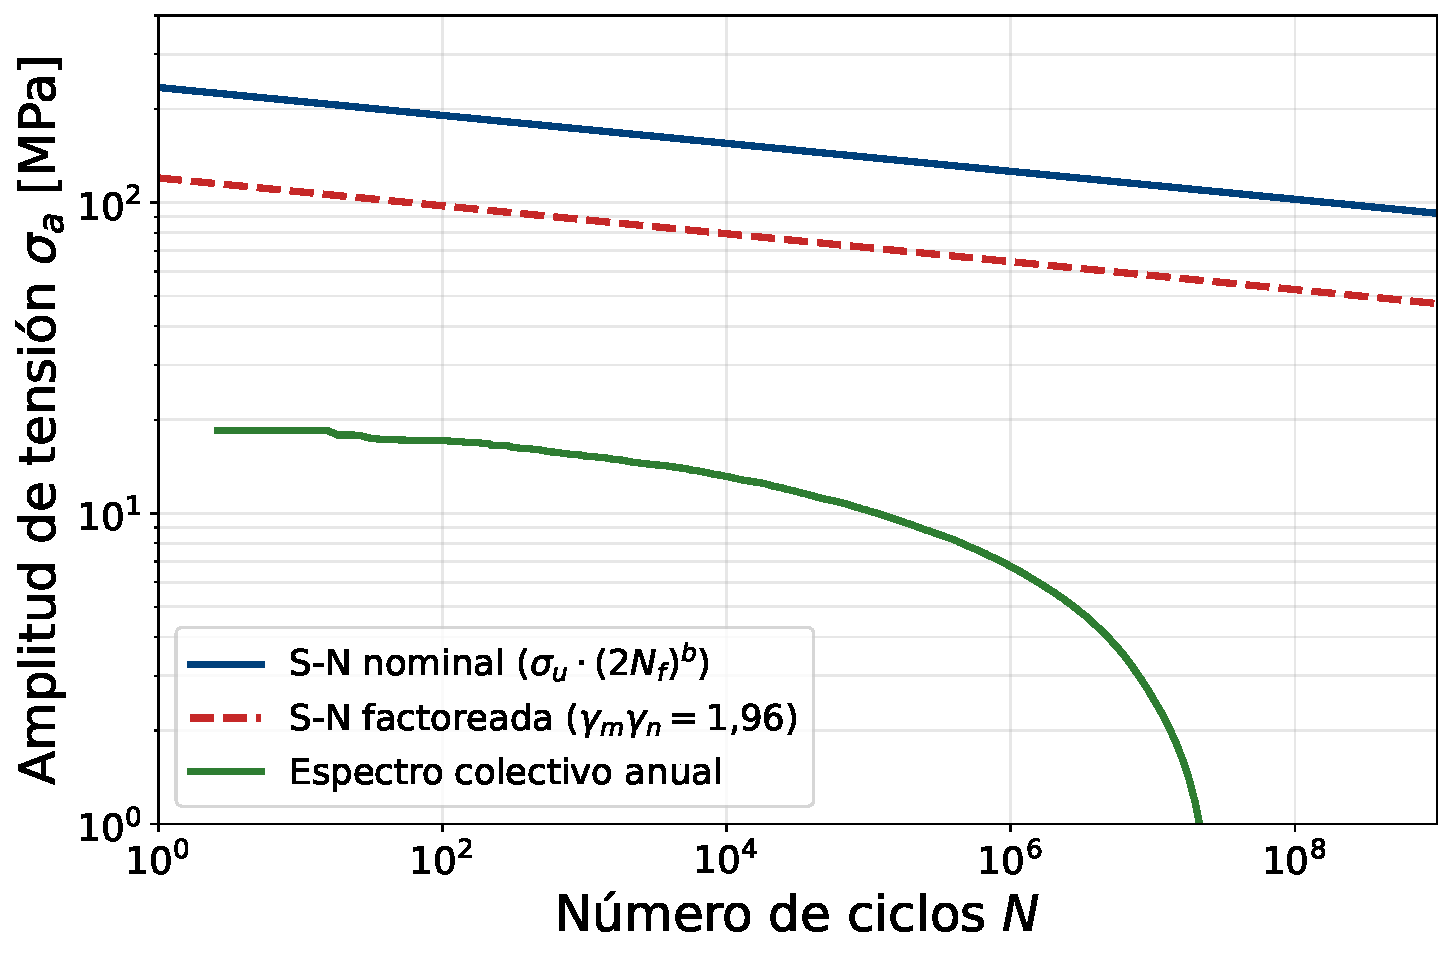
\includegraphics[width=0.95\textwidth]{Figuras/Figuras Resultados/curva_sn_gfrp.pdf}
    \caption{Curva S-N del GFRP $\pm 45^\circ$ en su forma nominal y factoreada, y espectro colectivo anual de fatiga.}
    \label{fig:curva_sn_gfrp}
\end{figure}

La superposición de ambas curvas en un mismo gráfico permite apreciar directamente el margen de seguridad a fatiga, ya que el espectro colectivo se sitúa por debajo de la curva S-N factoreada en todo el rango de ciclos. Las mayores amplitudes del espectro, que no superan los $18{,}4$~MPa, corresponden a las velocidades de viento más altas y a un número reducido de ciclos anuales, mientras que la gran mayoría de los ciclos se concentra en amplitudes de pocos MPa. Esas amplitudes se superponen a una tensión media elevada, comprendida entre $114{,}5$ y $135{,}4$~MPa, que impone la carga permanente de rotación y que sitúa los ciclos en régimen de tracción-tracción, con una razón de tensiones media de $R \approx 0{,}88$.

\subsection{Daño acumulado por velocidad de viento}

El daño de cada ciclo se obtiene al confrontar su amplitud con la curva S-N, y su contribución anual, al ponderarlo por el escalamiento temporal de la Tabla~\ref{tab:weibull_fatiga}. La Figura~\ref{fig:daño_por_viento} presenta el reparto resultante entre las doce velocidades del rango operacional.

\begin{figure}[H]
    \centering
    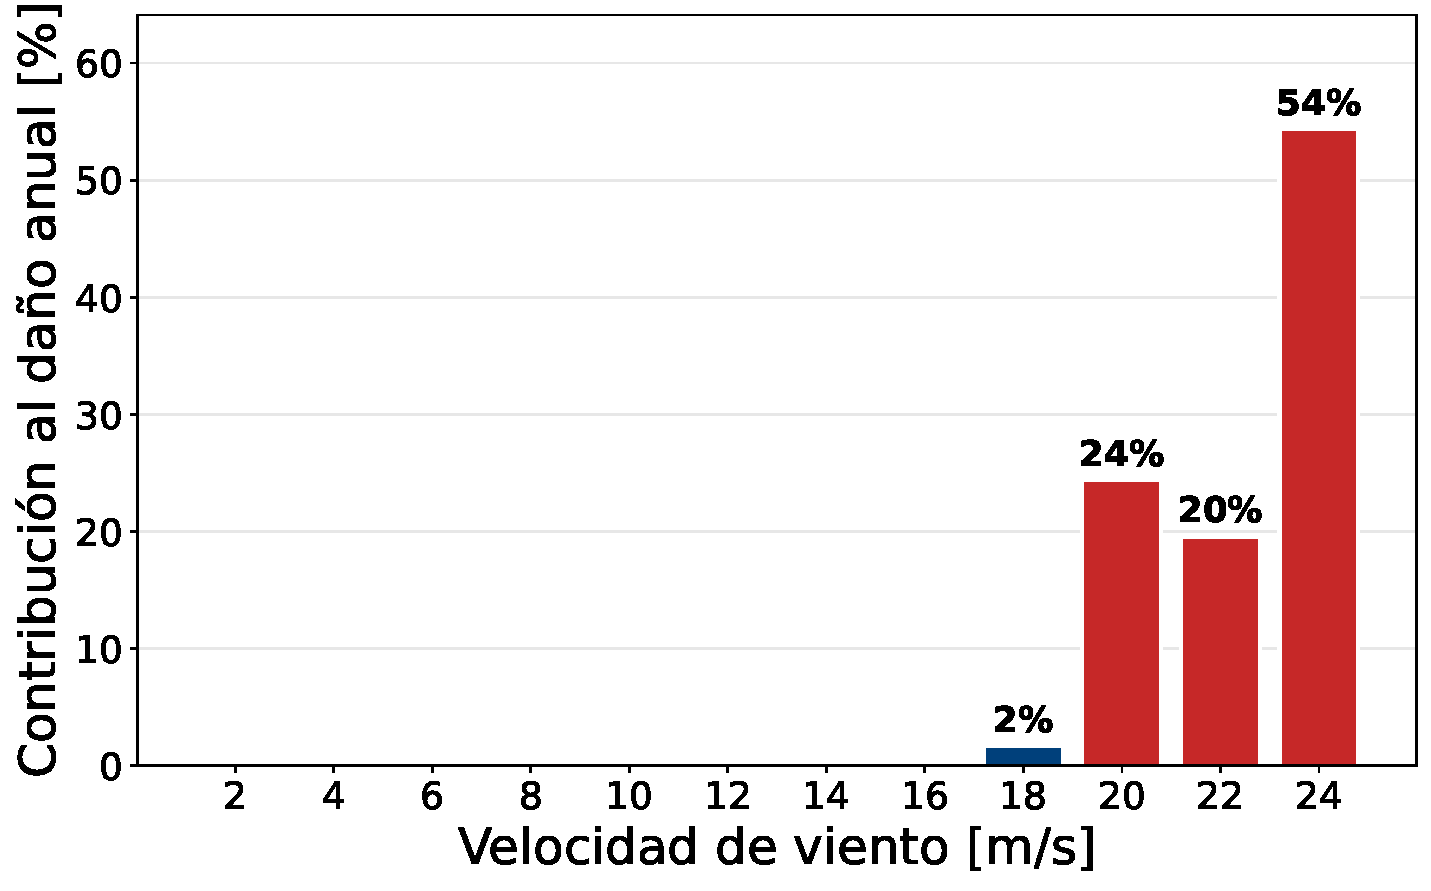
\includegraphics[width=0.7\textwidth]{Figuras/Figuras Resultados/daño_por_viento.pdf}
    \caption{Contribución porcentual de cada velocidad de viento al daño anual por fatiga.}
    \label{fig:daño_por_viento}
\end{figure}

El $98{,}3\%$ del daño se concentra en las tres velocidades más altas ($V = 20$--$24$~m/s) que, sin embargo, ocurren apenas el $0{,}8\%$ del año ($68$~h/año). El resultado es opuesto al que sugiere el factor de escalamiento y es característico de la fatiga en aerogeneradores~\parencite{Brondsted2005}, ya que la relación no lineal entre amplitud de tensión y daño ($D \propto \sigma_a^{|1/b|} = \sigma_a^{22{,}2}$) hace que los ciclos de mayor amplitud, aunque poco frecuentes, dominen el daño acumulado por sobre la frecuencia de ocurrencia.

\subsection{Daño acumulado total}

Sumando las contribuciones de las doce velocidades, el daño anual acumulado según la regla de Palmgren-Miner~\parencite{Miner1945} es $D_{\text{año}} = 3{,}22 \times 10^{-9}$. Para la vida útil de diseño de $20$ años, el daño total asciende al valor de la Ec.~\ref{eq:D20_res}:

\begin{equation}
    D_{20} = 20 \cdot D_{\text{año}} = 6{,}45 \times 10^{-8}
    \label{eq:D20_res}
\end{equation}

Este valor, muy por debajo del límite normativo de la Ec.~\ref{eq:fatiga_criterio}, indica que la fatiga no es un mecanismo dimensionante para la pala bajo las condiciones analizadas. La solicitación a fatiga se mantiene acotada por la combinación de dos factores. Primero, como muestra el espectro de la Figura~\ref{fig:curva_sn_gfrp}, las amplitudes de tensión no superan los $18{,}4$~MPa, en torno a un $8\%$ de $\sigma_u = 242{,}1$~MPa, ni siquiera en las condiciones más exigentes. Segundo, el exponente de Basquin $b = -0{,}045$, típico de tejidos biaxiales $\pm 45^\circ$ fabricados por infusión al vacío~\parencite{Huh2012}, produce una curva S-N excepcionalmente plana, cuya resistencia a fatiga decae muy lentamente con el número de ciclos, por lo que se requieren amplitudes de tensión cercanas a la resistencia última para generar daño significativo.

Conviene acotar el alcance de esa cifra. Un daño de $6{,}45 \times 10^{-8}$ proviene de extrapolar la curva de Basquin muy por encima del rango de ciclos ensayado por \textcite{Huh2012}, de modo que su magnitud exacta no admite lectura literal como predicción de vida. La verificación admite, en cambio, una cota que no depende de esa extrapolación. El ciclo más severo de toda la campaña, de amplitud $18{,}4$~MPa sobre una media de $135{,}4$~MPa, corregido por Goodman y factorado, equivale a una amplitud de diseño de $81{,}8$~MPa, a la que la curva S-N asigna $N_f = 1{,}49 \times 10^{10}$ ciclos. El rotor completa $4{,}42 \times 10^{8}$ revoluciones en los $20$ años de vida de diseño girando a su velocidad máxima, de modo que aun bajo el supuesto extremo de que todos esos ciclos fueran el más severo registrado, el daño acumulado alcanzaría $D_{20} = 0{,}030$, todavía por debajo de la unidad. La verificación a fatiga se satisface, por tanto, con independencia del tramo extrapolado de la curva.

El margen a fatiga no habilita, sin embargo, una reducción del espesor de pared, ya que, como se verá en la Sección~\ref{sec:resultados_fem}, la verificación de estabilidad demanda rigidización adicional de la piel, no menos material. La fatiga queda así descartada como criterio dimensionante, y el diseño pasa a estar gobernado por la estabilidad y, en segundo término, por la resistencia última.

\section{Verificación estructural de la pala}
\label{sec:resultados_fem}

Las fuerzas de diseño por estación de la Sección~\ref{sec:comparacion_dlc}, junto con la aceleración centrífuga, constituyen las cargas del modelo de elementos finitos descrito en la Sección~\ref{sec:fem}. Su resolución se aborda en tres pasos: primero se verifica que los resultados sean independientes de la discretización, luego se describen las condiciones de borde y cargas aplicadas, y finalmente se presentan las tensiones y deformaciones de los DLC 1.1 y 1.3, con las que se evalúan los criterios de resistencia última, estabilidad y deflexión de la norma IEC 61400-1~\parencite{IEC61400-1}.

\subsection{Convergencia de malla}

La independencia de los resultados respecto del tamaño de elemento se verifica mediante un análisis de convergencia con cinco tamaños de elemento, desde $20$~mm hasta $12$~mm de tamaño característico, sobre el caso DLC 1.1. La Figura~\ref{fig:convergencia_malla} presenta la evolución de la tensión principal máxima en función del tamaño de elemento y la Tabla~\ref{tab:convergencia_malla} resume los valores obtenidos y la variación porcentual entre mallas consecutivas.

\begin{figure}[H]
    \centering
    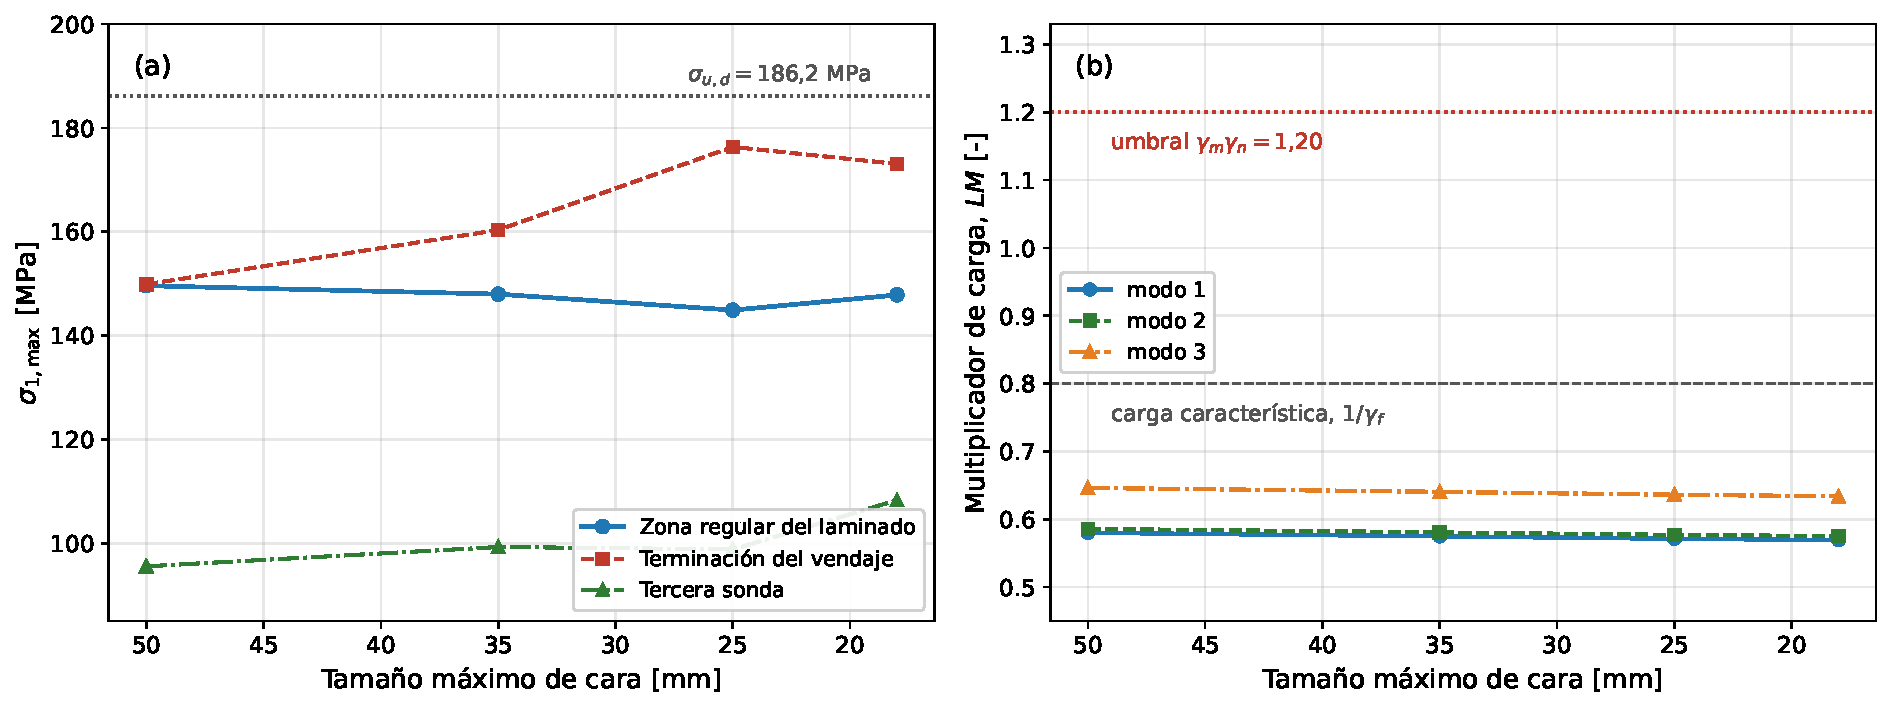
\includegraphics[width=0.65\textwidth]{Figuras/Figuras Resultados/convergencia_malla.pdf}
    \caption{Convergencia de malla, tensión principal máxima $\sigma_{1,\text{max}}$ en función del tamaño característico de elemento.}
    \label{fig:convergencia_malla}
\end{figure}

\begin{table}[H]
    \centering
    \caption{Análisis de convergencia de malla para cinco tamaños de elemento.}
    \label{tab:convergencia_malla}
    \begin{tabular}{lcccccc}
        \hline
        \textbf{Tamaño (mm)} & $\sigma_{1,\max}$ \textbf{(MPa)} & $\Delta\sigma_1$ \textbf{(\%)} & $\sigma_{3,\min}$ \textbf{(MPa)} & $\Delta\sigma_3$ \textbf{(\%)} & $\mathbf{F_{s1}}$ \textbf{(kN)} & $\mathbf{F_{s2}}$ \textbf{(kN)} \\
        \hline
        $20$ & $151{,}6$ & ---      & $-121{,}7$ & ---      & $153{,}26$ & $151{,}55$ \\
        $18$ & $153{,}8$ & $1{,}45$ & $-122{,}6$ & $0{,}69$ & $153{,}29$ & $151{,}58$ \\
        $16$ & $159{,}5$ & $3{,}66$ & $-124{,}5$ & $1{,}55$ & $153{,}31$ & $151{,}60$ \\
        $14$ & $162{,}2$ & $1{,}70$ & $-125{,}5$ & $0{,}87$ & $153{,}31$ & $151{,}60$ \\
        $12$ & $163{,}4$ & $0{,}76$ & $-127{,}1$ & $1{,}21$ & $153{,}31$ & $151{,}60$ \\
        \hline
    \end{tabular}
\end{table}

La diferencia en la tensión principal máxima entre las dos mallas más finas ($14$~mm y $12$~mm) es del $0{,}76\%$, muy por debajo del criterio del $5\%$ adoptado en este trabajo (Sección~\ref{sec:fem}). Este margen holgado respecto al umbral de la literatura~\parencite{Qin2026,Hameed2015,Boudounit2020} indica que la malla de $12$~mm resuelve adecuadamente los gradientes de tensión en la zona de interés, particularmente en las conexiones strut--pala donde se concentran las máximas solicitaciones. Las fuerzas de reacción en ambos struts presentan variaciones inferiores al $0{,}04\%$ en todas las mallas, confirmando que el equilibrio global de fuerzas es independiente de la discretización. Se selecciona el tamaño de elemento de $12$~mm para las simulaciones definitivas.

La malla definitiva presenta una calidad de elemento media (\textit{element quality}) de $0{,}9893$. Esta métrica de Ansys toma el valor $1$ para un elemento de forma ideal, por lo que el valor obtenido indica que la práctica totalidad de los elementos conserva una geometría próxima a la óptima, sin zonas de distorsión que pudieran degradar localmente la solución.

\subsection{Modelo de elementos finitos}

La Figura~\ref{fig:fem_cb} muestra el modelo con las condiciones de borde que define la Sección~\ref{sec:condiciones_borde}, esto es, los empotramientos en las dos conexiones con los brazos y la aceleración centrífuga aplicada radialmente sobre todos los elementos de la pala.

\begin{figure}[H]
    \centering
    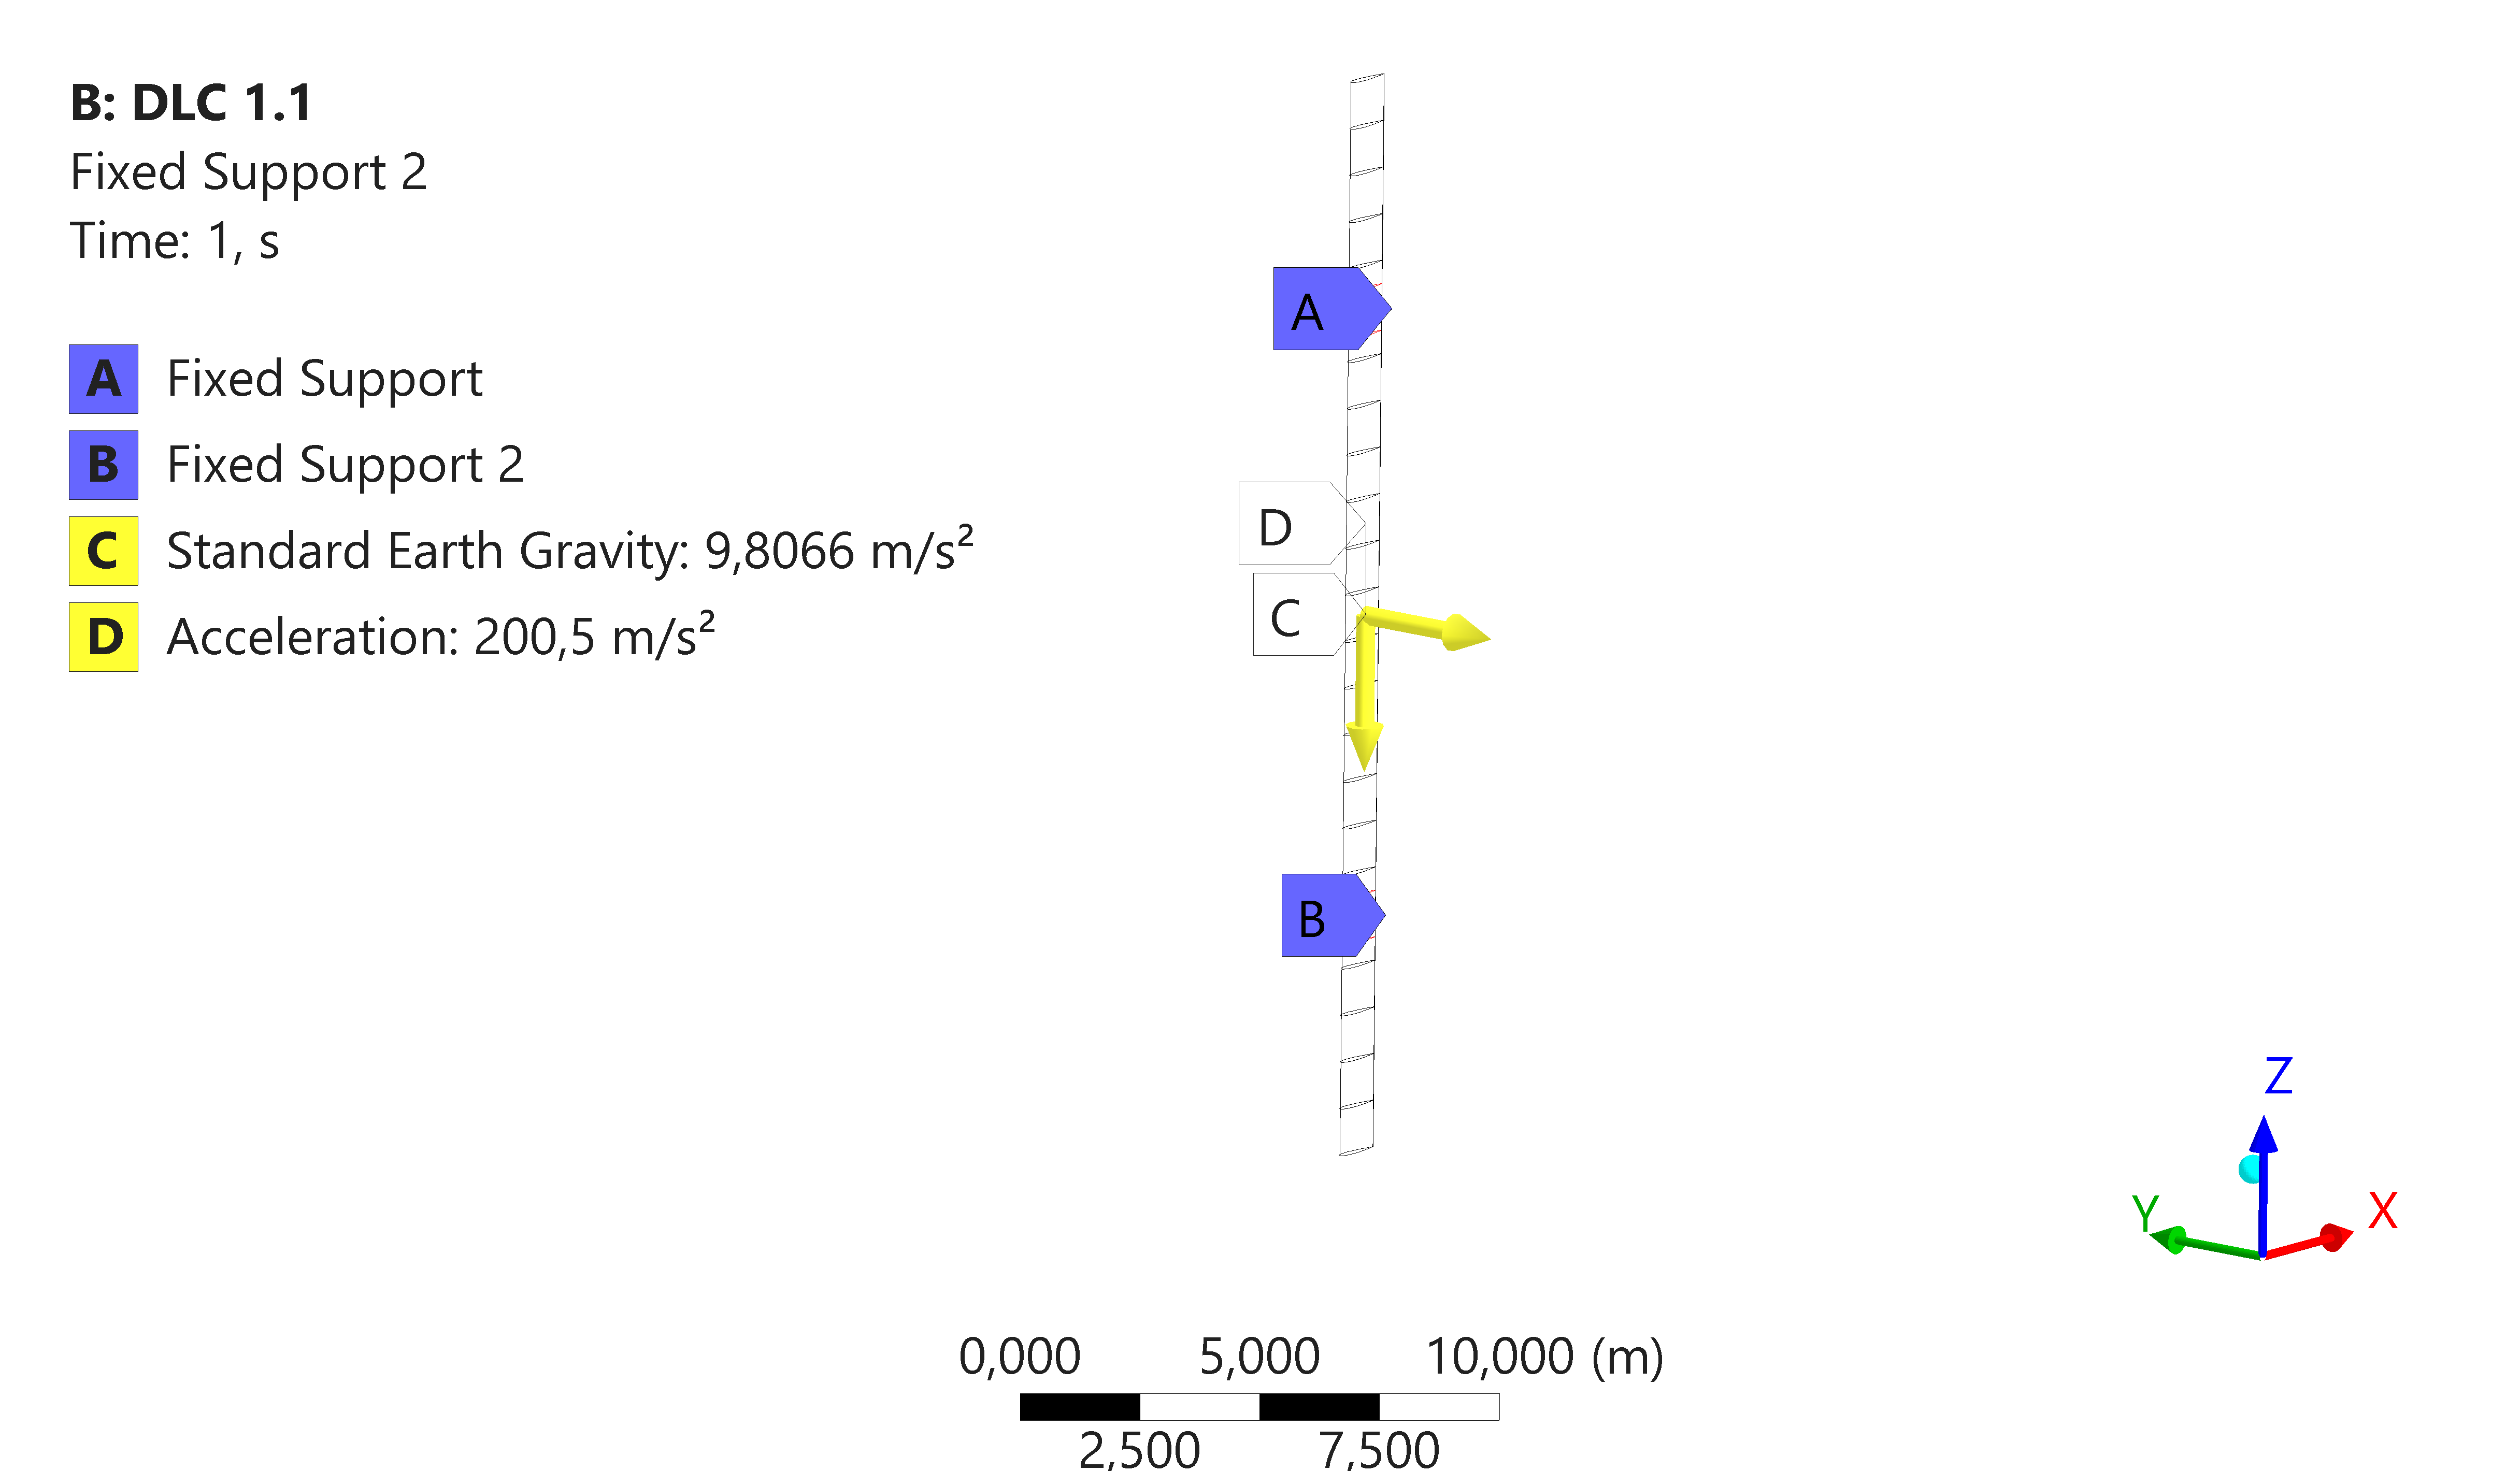
\includegraphics[width=\textwidth]{Figuras/Figuras Resultados/fem_cb.png}
    \caption{Condiciones de borde del modelo FEM, empotramientos en los dos puntos de conexión con los struts y aceleración centrífuga radial.}
    \label{fig:fem_cb}
\end{figure}

La aceleración centrífuga corresponde a la velocidad máxima de rotación $\Omega = 42$~rpm ($4{,}398$~rad/s) que, evaluada en la Ec.~\ref{eq:centrifugal_limit} con $R = 10{,}365$~m, resulta en $a_c = 200{,}5$~m/s$^2$ ($20{,}4\,g$), uniforme en toda la envergadura. Esa magnitud sitúa en su justa dimensión la consigna de $42$~rpm. Como la aceleración centrífuga es inversamente proporcional al radio (Ec.~\ref{eq:centrifugal_limit}), el menor radio del rotor en estudio implica una solicitación centrífuga un $29\%$ superior a la de la T1-turbine en su límite de diseño~\parencite{Mollerstrom2017}, pese a que ambas máquinas comparten la misma velocidad de punta. La admisibilidad de la consigna no se sustenta por tanto en la comparación con la literatura, sino en la verificación estructural que se desarrolla en esta sección.

La Figura~\ref{fig:fem_fuerzas} muestra las fuerzas aerodinámicas de diseño $F_d$ del DLC 1.1 aplicadas como cargas remotas en los centroides de las 24 estaciones, conservando el signo del instante gobernante (Sección~\ref{sec:anexo_f}), en el cual la componente normal a la cuerda apunta hacia el extradós, coincidiendo con el sentido de la flexión inducida por la fuerza centrífuga, condición que hace de este el estado combinado más desfavorable.

\begin{figure}[H]
    \centering
    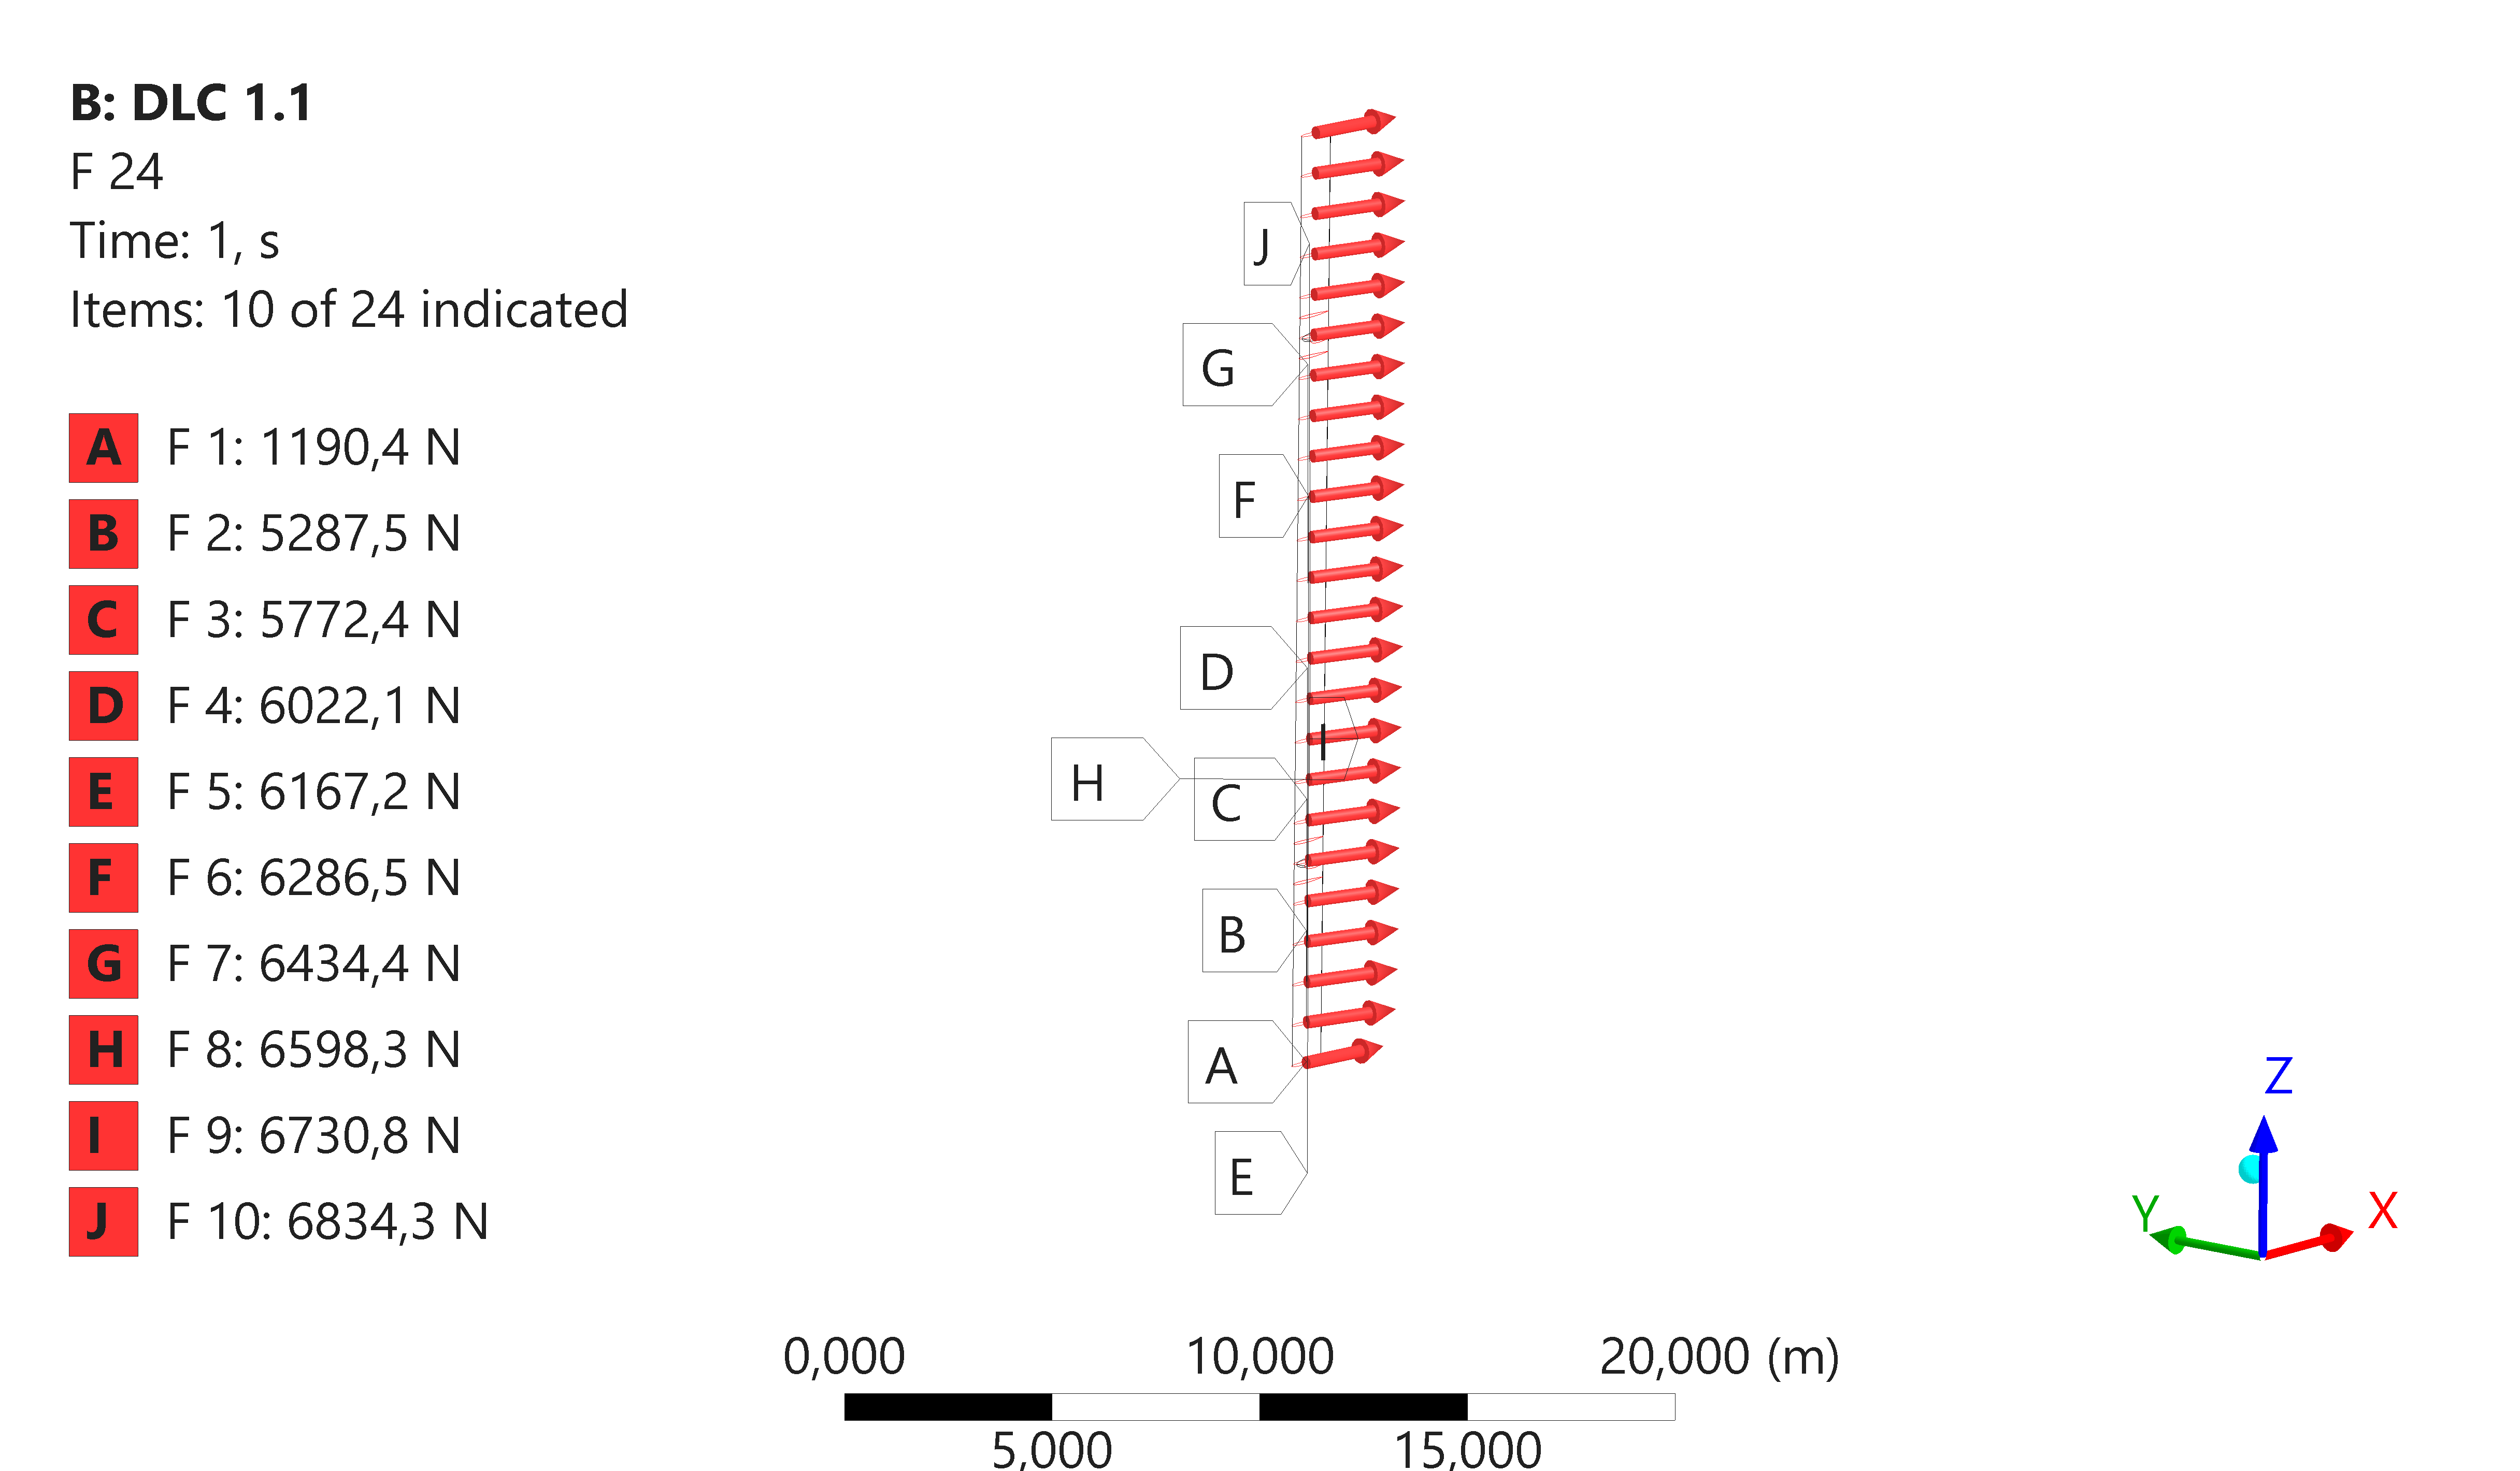
\includegraphics[width=\textwidth]{Figuras/Figuras Resultados/fem_fuerzas.png}
    \caption{Fuerzas aerodinámicas de diseño aplicadas como cargas remotas en las 24 estaciones de la pala.}
    \label{fig:fem_fuerzas}
\end{figure}

La Figura~\ref{fig:fem_detalle_union} presenta el detalle constructivo de la unión entre la pala y el brazo de soporte tal como queda resuelta en el modelo. Se distinguen en ella sus tres elementos, el vendaje de refuerzo de la zona de conexión y la superficie de apoyo sobre la que se imponen los empotramientos (Sección~\ref{sec:condiciones_borde}), y el larguero interior de $8$~mm alojado en la zona de espesor máximo del perfil (Sección~\ref{sec:material_pala}).


\begin{figure}[H]
    \centering
    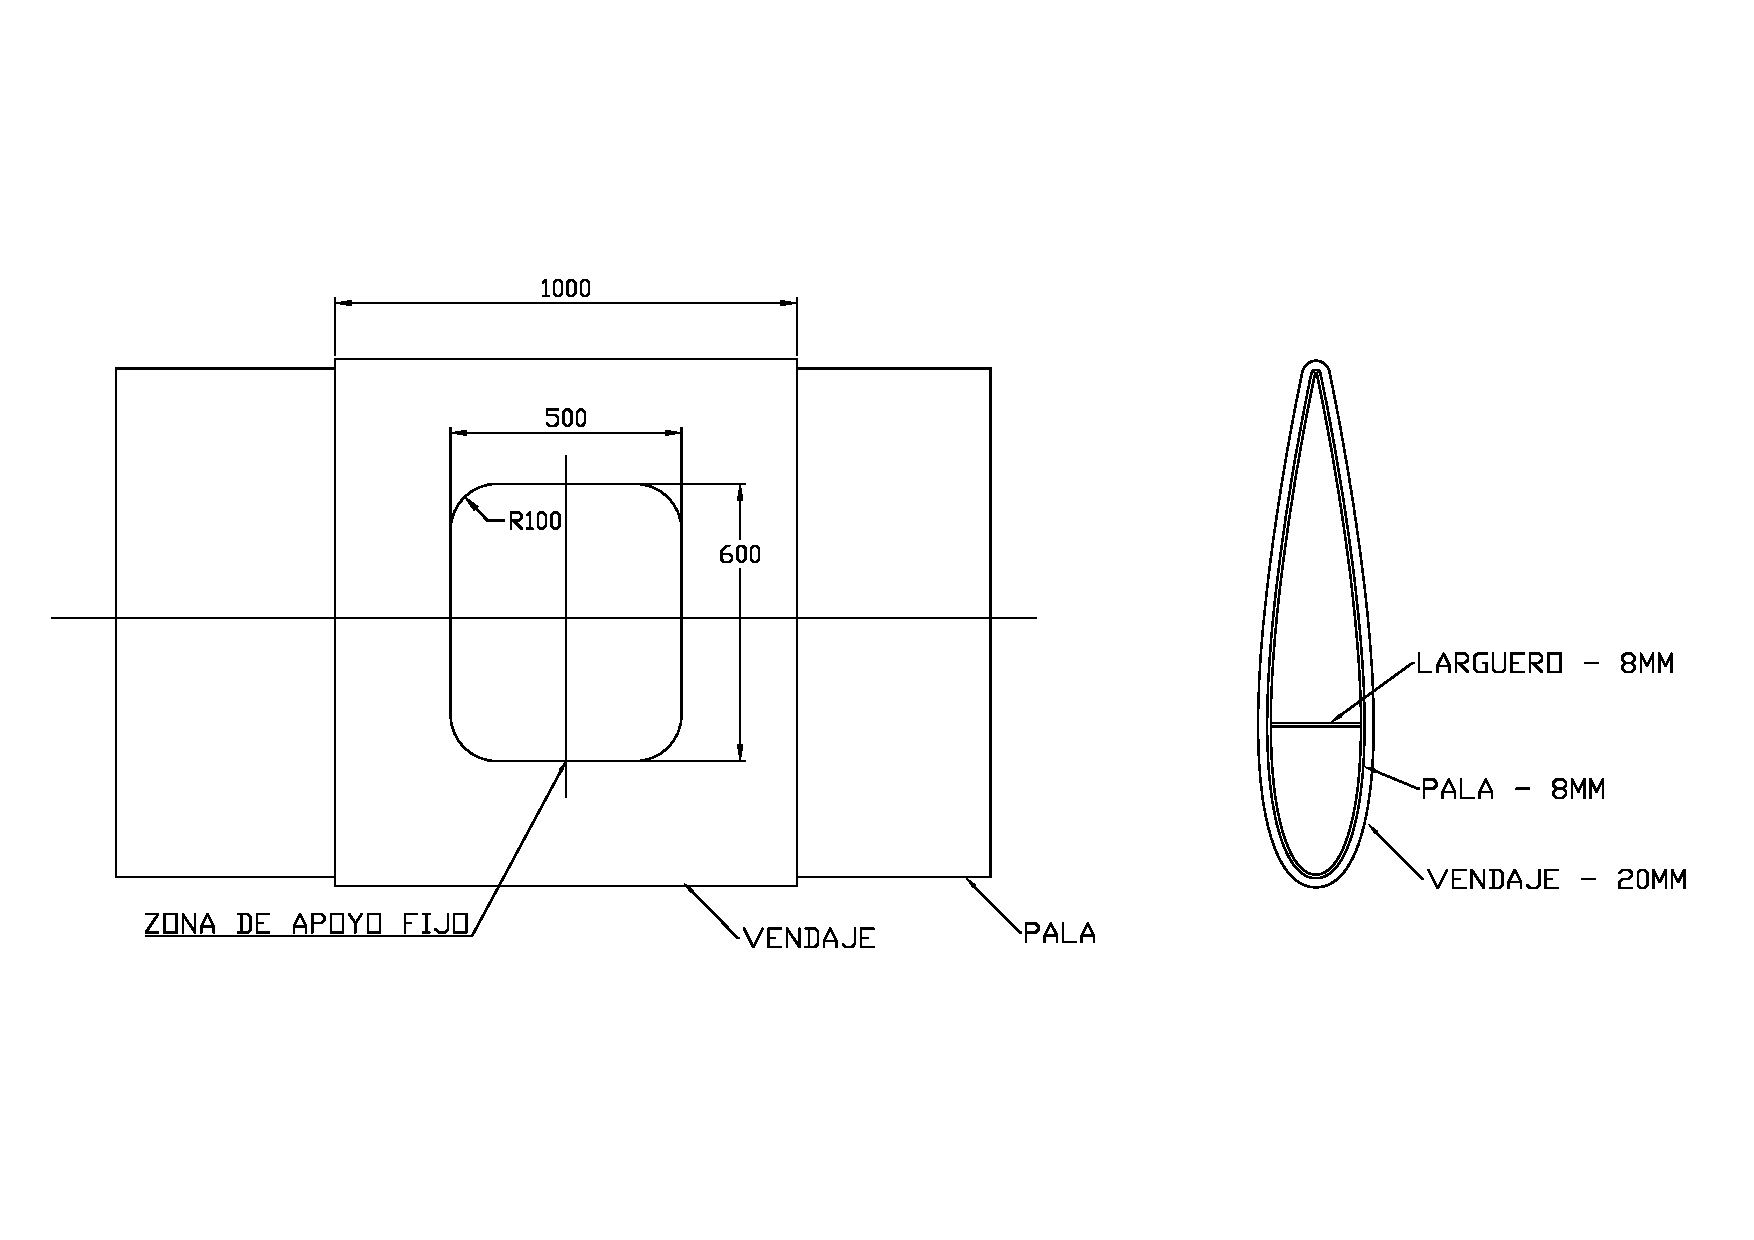
\includegraphics[trim=0cm 3cm 0cm 3cm, clip, width=0.85\textwidth]{Figuras/Figuras Resultados/PLANO.pdf}
    \caption{Detalle de la unión pala-brazo modelada en el FEM.}
    \label{fig:fem_detalle_union}
\end{figure}

\subsection{Resultados del análisis estructural}

Se reportan primero las tensiones y la deformación bajo las cargas del DLC 1.1, caso gobernante de la resistencia última, y a continuación las correspondientes al DLC 1.3. Adicionalmente, se presenta un caso de referencia resuelto únicamente con las cargas inerciales (aceleración centrífuga y gravedad, sin fuerzas aerodinámicas), que permite cuantificar la contribución de la rotación al estado tensional.

\subsubsection{Tensiones principales}

La Figura~\ref{fig:fem_max11} presenta la distribución de tensión principal máxima en ambas caras de la pala (intradós y extradós), junto con un detalle de la zona crítica. El valor máximo $\sigma_{1,\max} = 163{,}4$~MPa se localiza en la zona de conexión con el strut inferior ($z = 5$~m).

\begin{figure}[H]
    \centering
    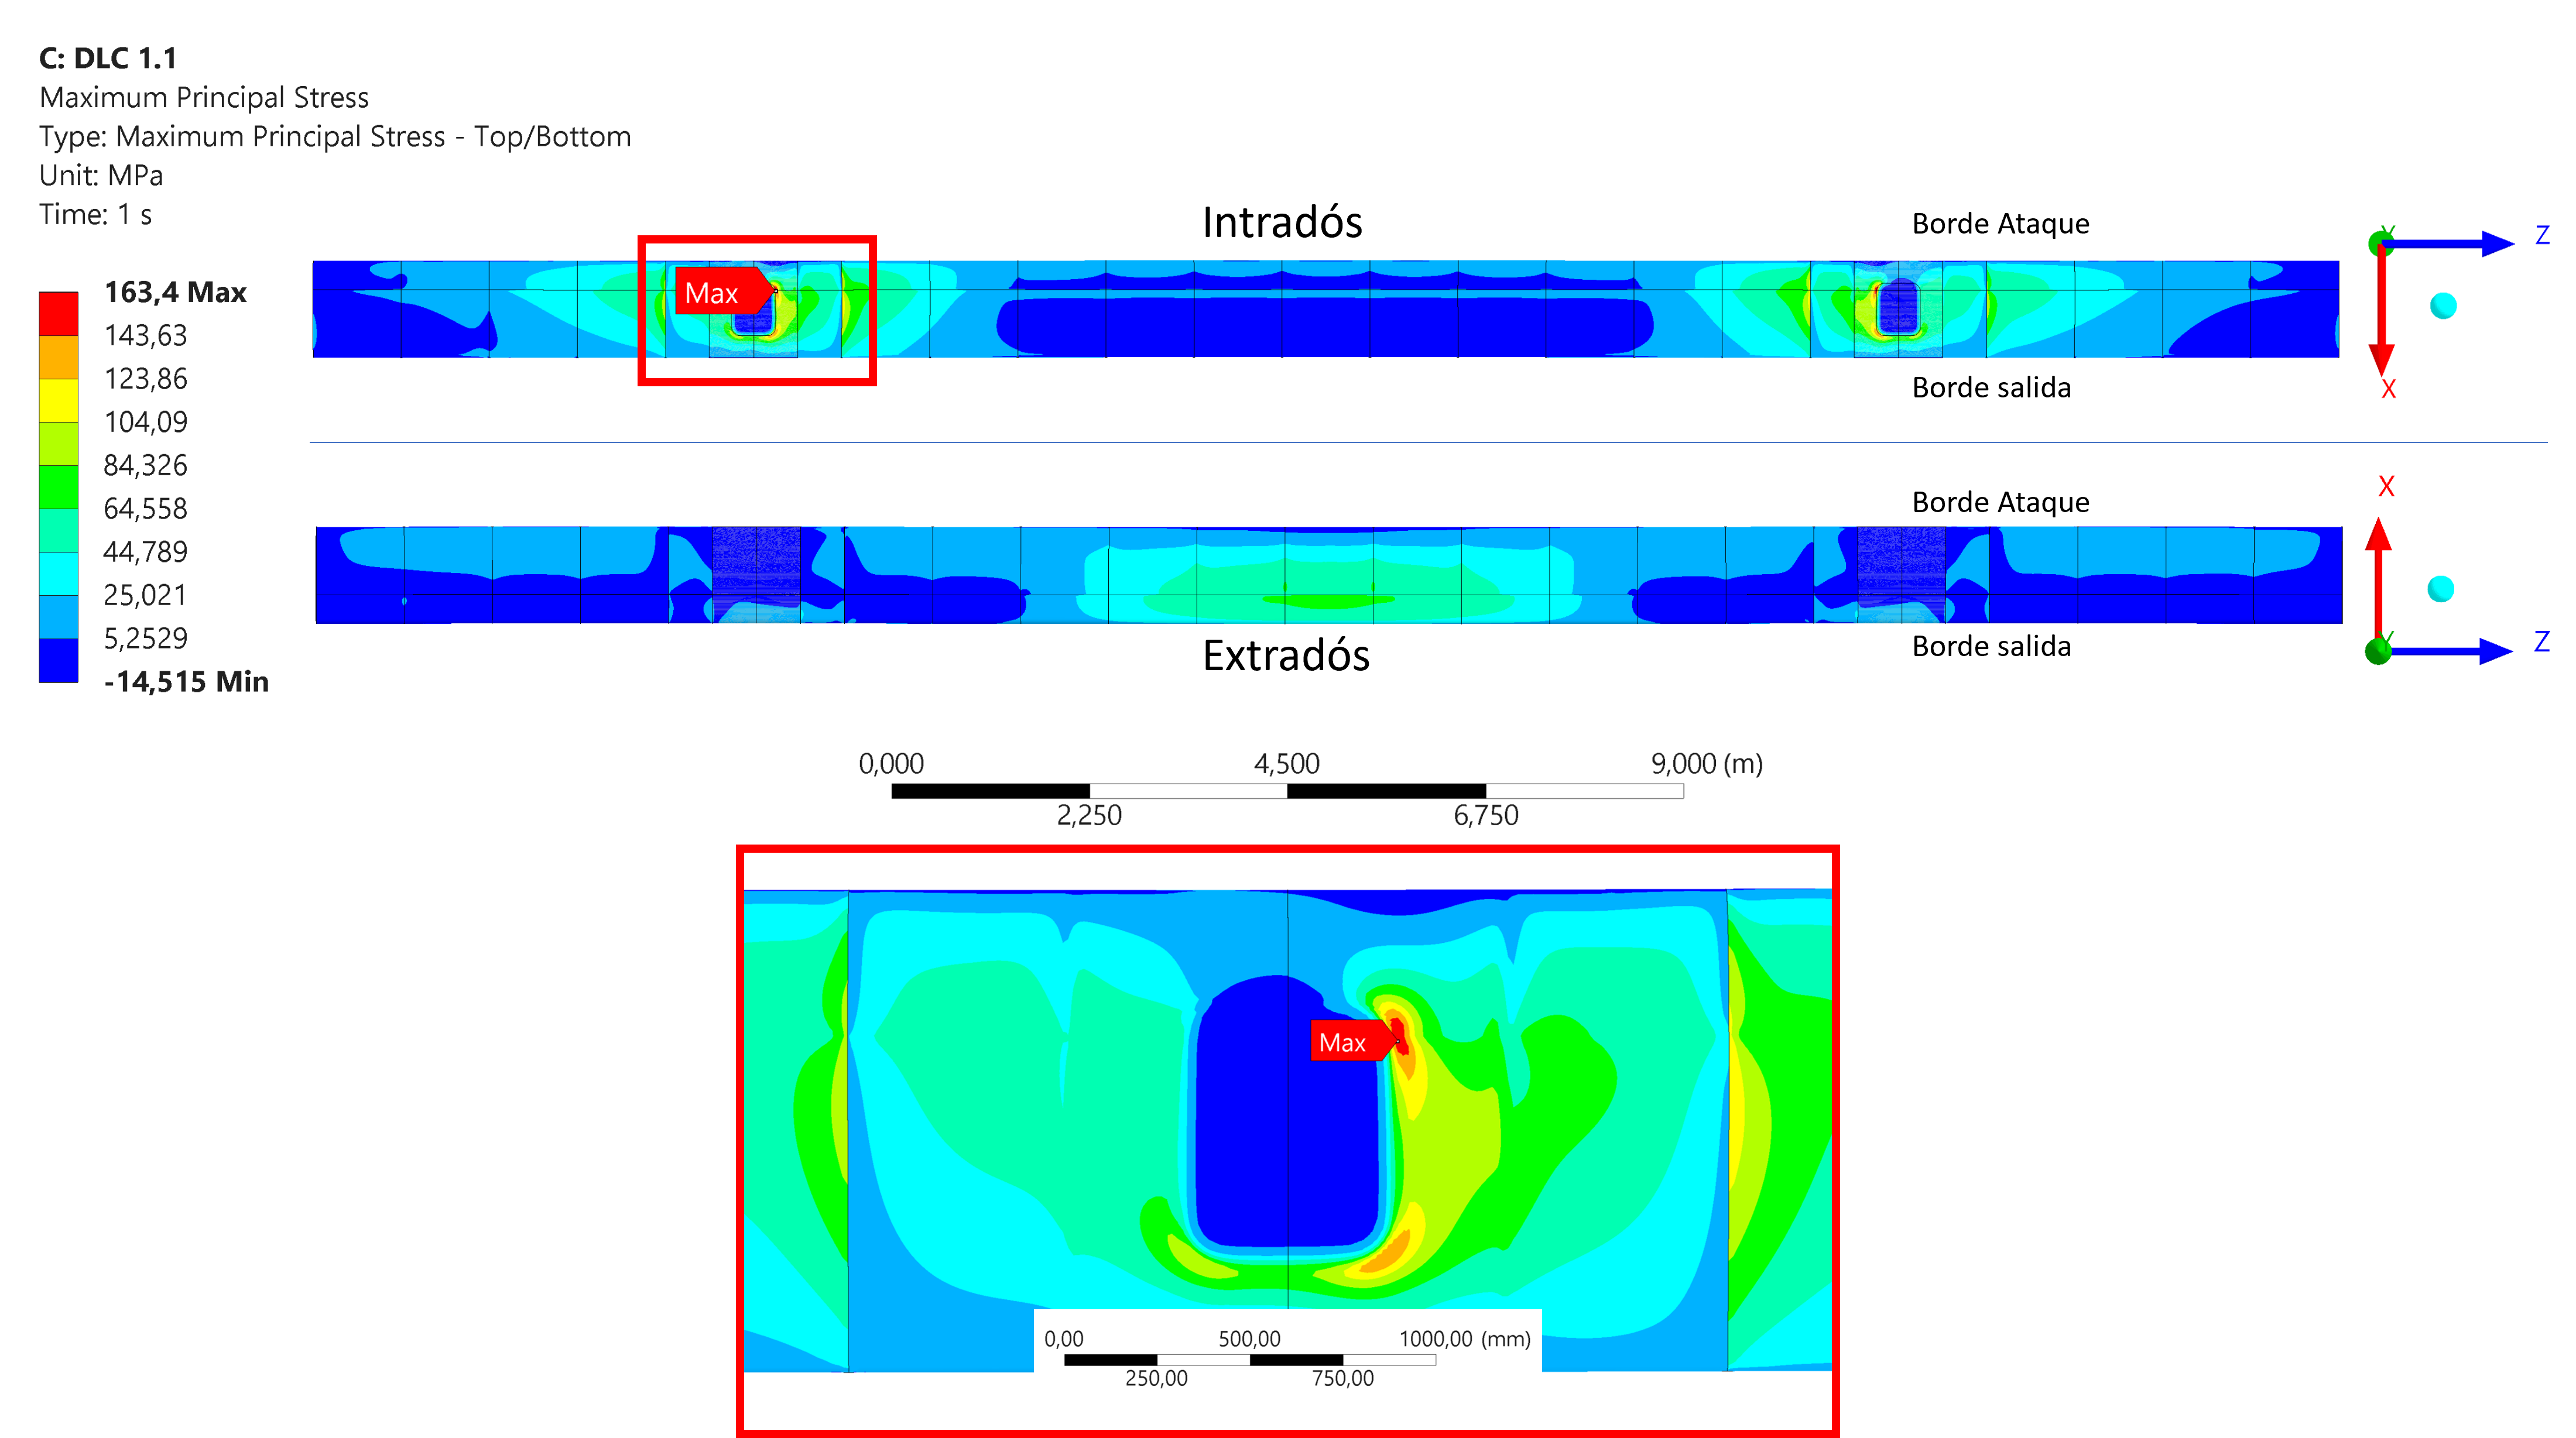
\includegraphics[width=\textwidth]{Figuras/Figuras Resultados/fem_max11.png}
    \caption{Distribución de tensión principal máxima, DLC 1.1.}
    \label{fig:fem_max11}
\end{figure}

Conviene precisar el alcance de ese valor. Ante la falta de un plano de la unión, el soporte se representó mediante una superficie de apoyo al final del brazo, reforzada por un vendaje (Sección~\ref{sec:condiciones_borde}), y es justamente en esa zona donde el modelo localiza el máximo. La tensión obtenida responde, por tanto, tanto a la solicitación como a la geometría supuesta para la unión. El análisis de convergencia descarta que el concentrador provenga de la discretización, ya que la tensión varía un $0{,}76\%$ entre las dos mallas más finas, pero no puede descartar su sensibilidad al detalle constructivo, ya que una unión de mayor superficie de apoyo, con una transición más gradual hacia el laminado, redistribuiría la tensión en esa zona.

La Figura~\ref{fig:fem_min11} muestra la tensión principal mínima, $\sigma_{3,\min} = -127{,}1$~MPa, correspondiente a compresión en la zona de las conexiones. Este estado de tracción en una cara y compresión en la opuesta responde a la flexión inducida por las fuerzas aerodinámicas y la fuerza centrífuga, que en el instante de diseño actúan en el mismo sentido (Sección~\ref{sec:anexo_f}).

\begin{figure}[H]
    \centering
    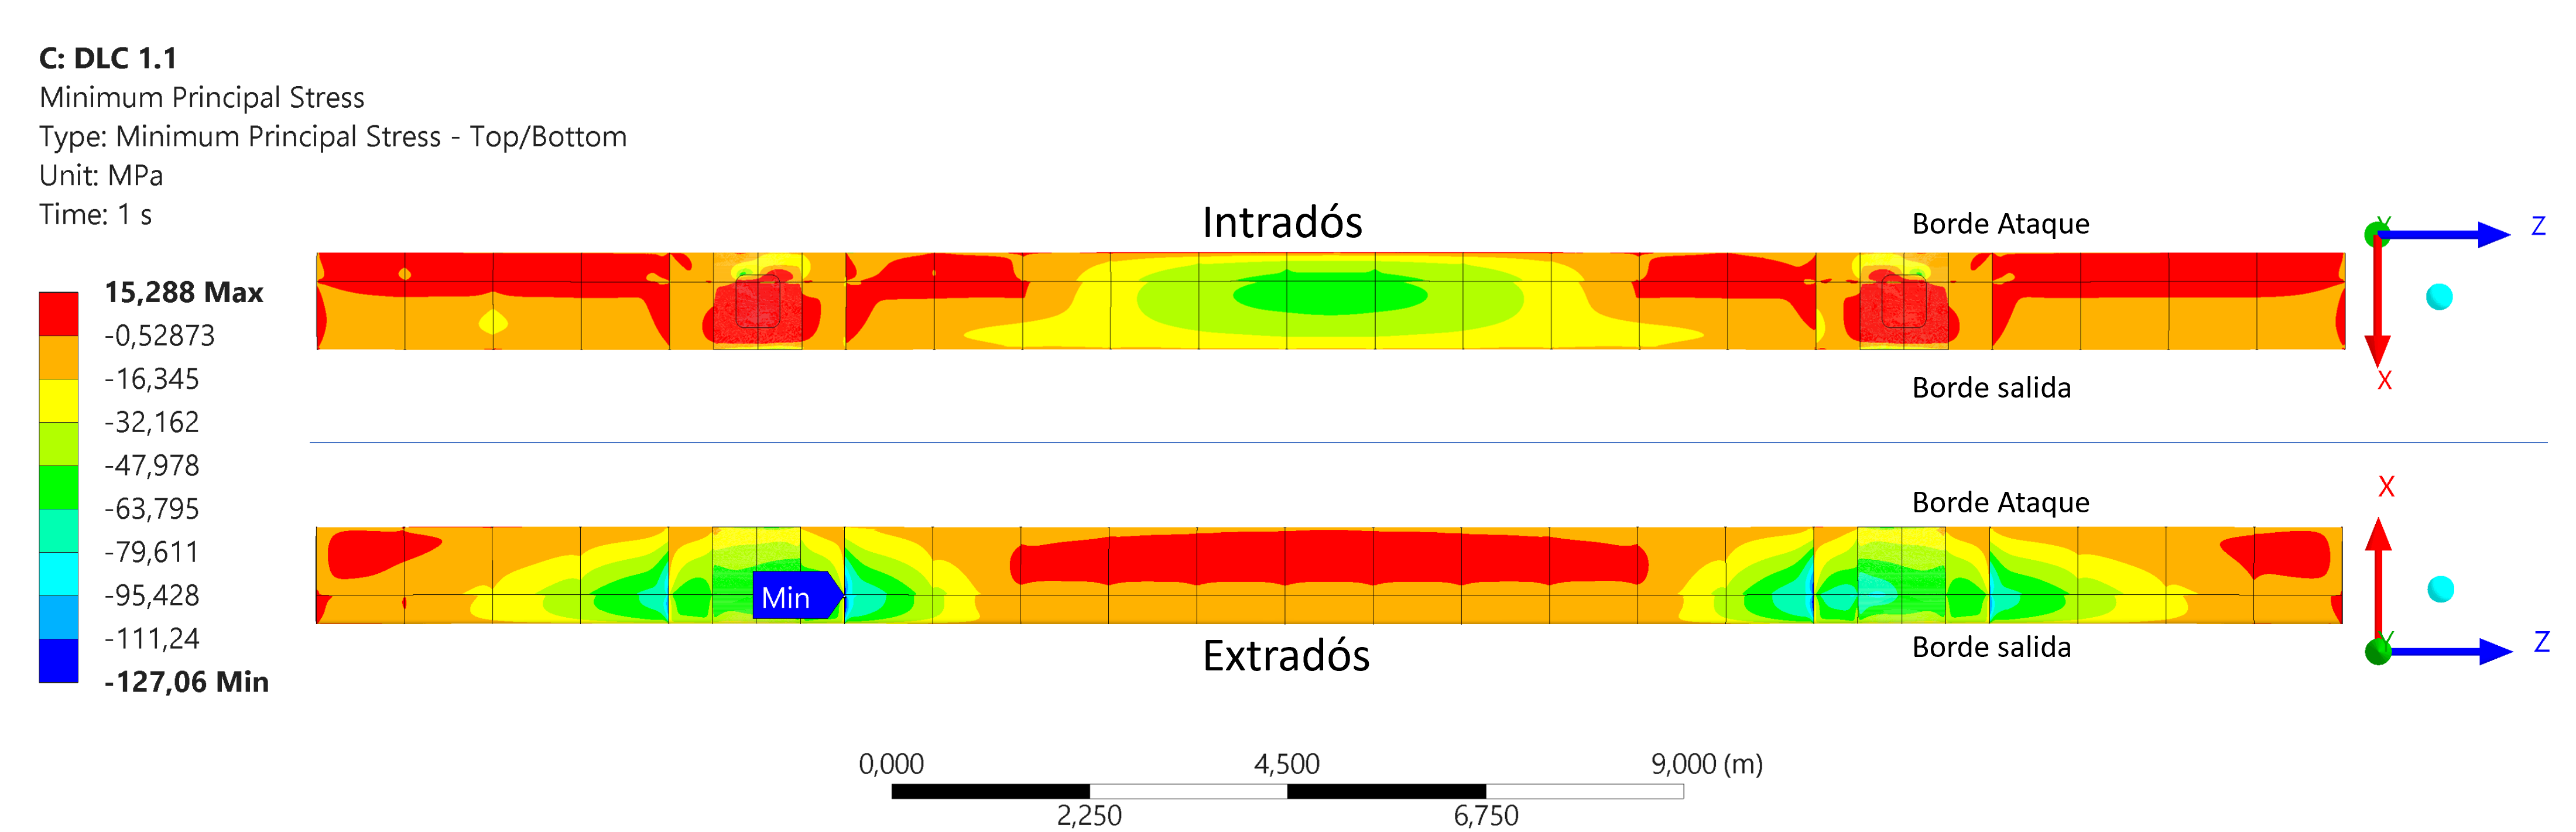
\includegraphics[width=\textwidth]{Figuras/Figuras Resultados/fem_min11.png}
    \caption{Distribución de tensión principal mínima, DLC 1.1.}
    \label{fig:fem_min11}
\end{figure}

\subsubsection{Deformación}

La Figura~\ref{fig:fem_deformacion11} presenta la deformación total de la pala bajo las cargas de diseño del DLC 1.1. La deformación máxima es de $0{,}169$~m y ocurre en la zona central de la pala, entre ambos apoyos, donde la flexión del vano alcanza su flecha máxima.

\begin{figure}[H]
    \centering
    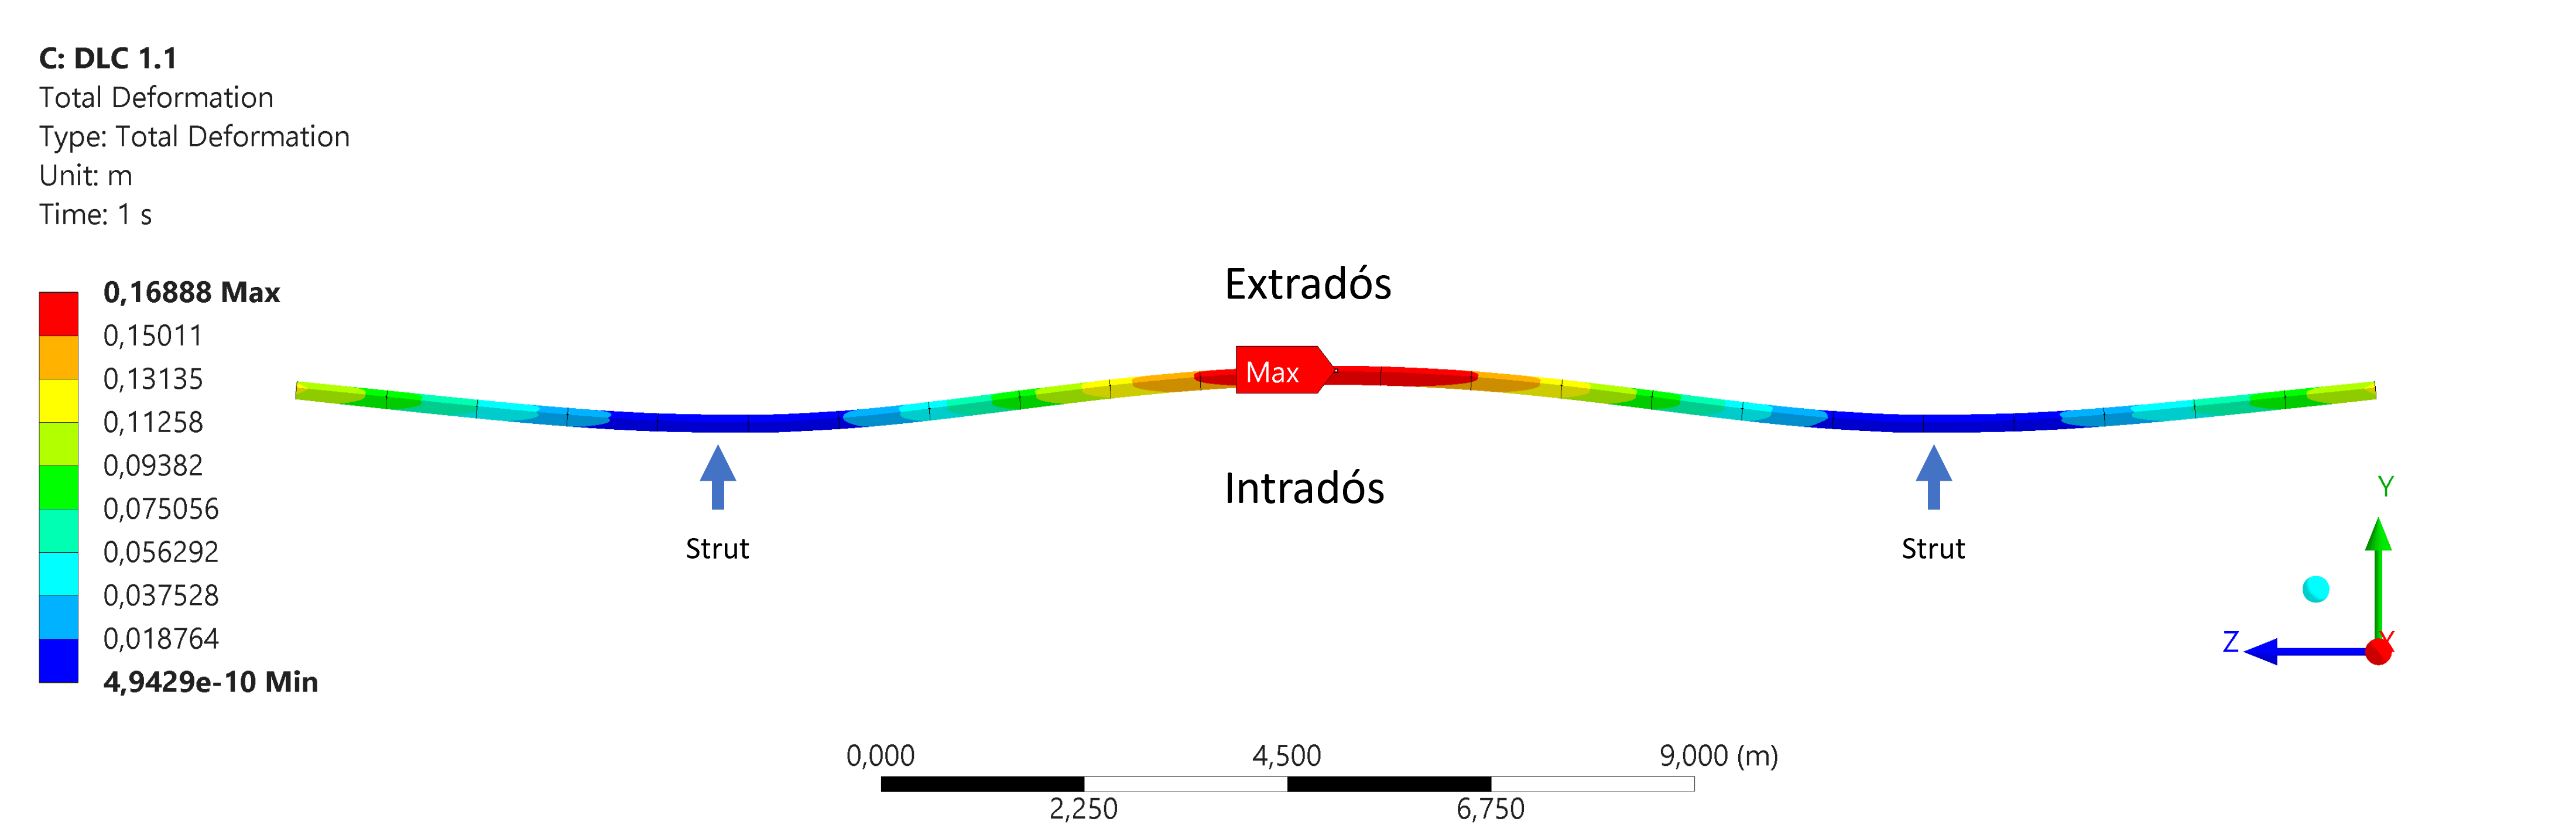
\includegraphics[width=\textwidth]{Figuras/Figuras Resultados/fem_deformacion11.png}
    \caption{Deformación total, DLC 1.1.}
    \label{fig:fem_deformacion11}
\end{figure}

\subsubsection{DLC 1.3}

Bajo las cargas de diseño del DLC 1.3, la distribución de tensión principal máxima (Figura~\ref{fig:fem_max13}) conserva el patrón del caso anterior, ya que el valor máximo, $\sigma_{1,\max} = 156{,}8$~MPa, vuelve a localizarse en la zona de las conexiones pala-brazo, lo que confirma que la ubicación de la sección crítica no depende del caso de carga.

\begin{figure}[H]
    \centering
    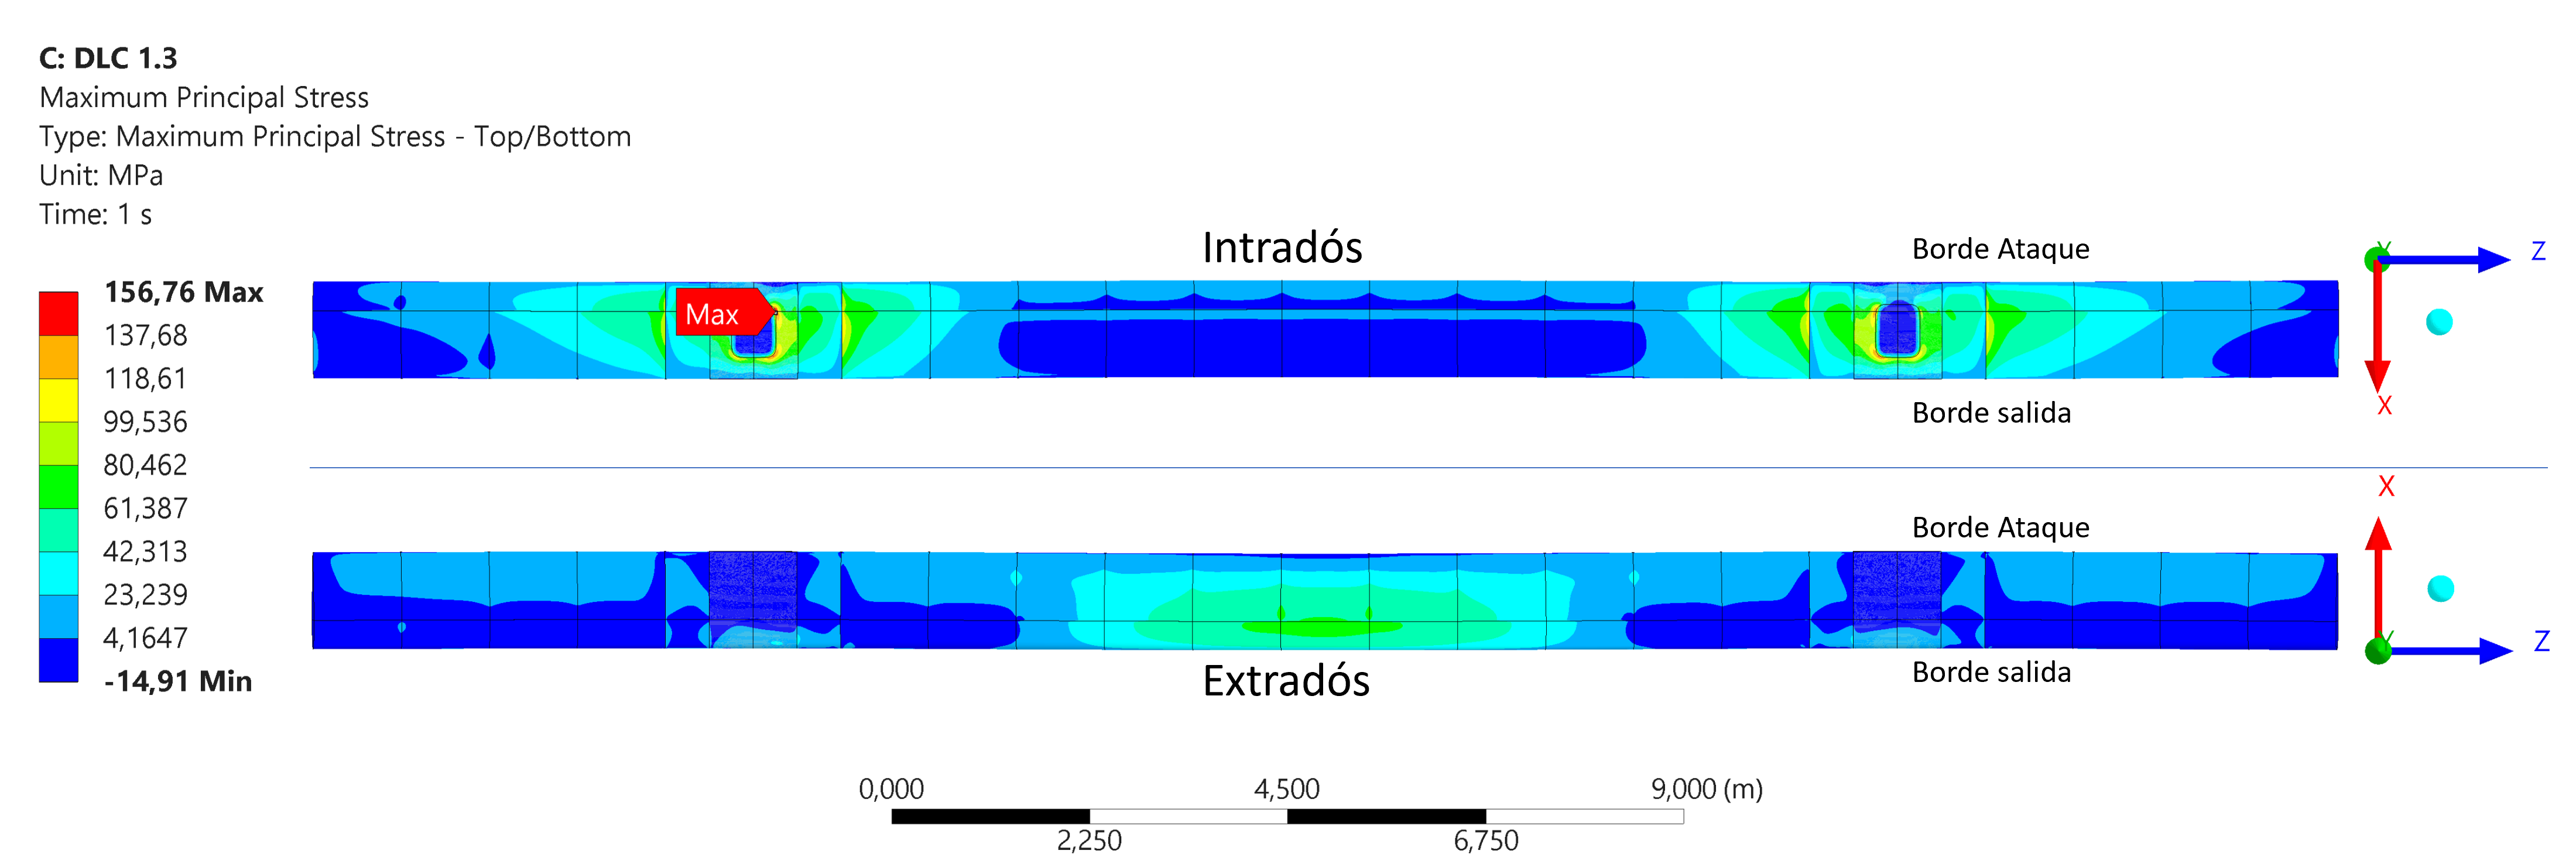
\includegraphics[width=\textwidth]{Figuras/Figuras Resultados/fem_max13.png}
    \caption{Distribución de tensión principal máxima, DLC 1.3.}
    \label{fig:fem_max13}
\end{figure}

En compresión, la tensión principal mínima (Figura~\ref{fig:fem_min13}) alcanza $\sigma_{3,\min} = -129{,}4$~MPa, en este caso de magnitud levemente mayor que la del DLC 1.1 ($-127{,}1$~MPa).

\begin{figure}[H]
    \centering
    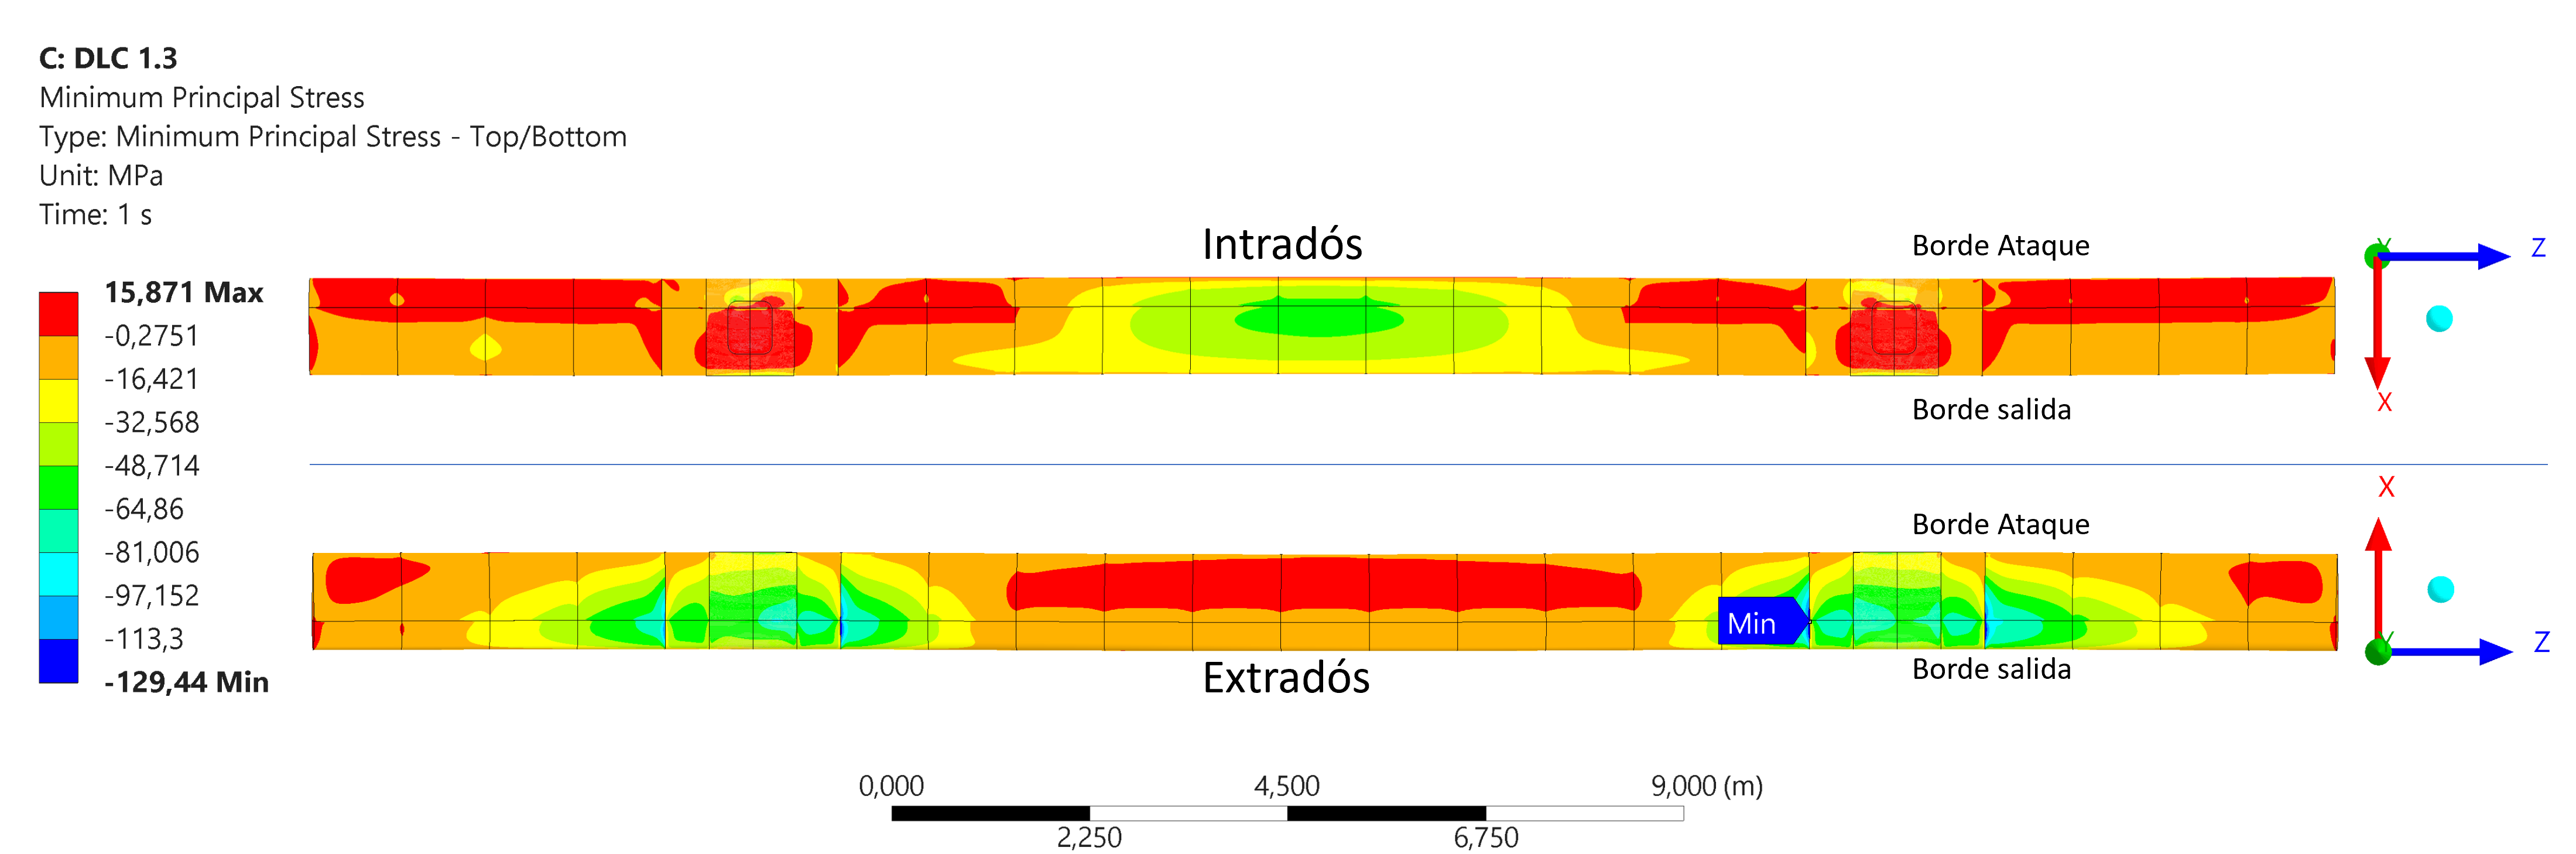
\includegraphics[width=\textwidth]{Figuras/Figuras Resultados/fem_min13.png}
    \caption{Distribución de tensión principal mínima, DLC 1.3.}
    \label{fig:fem_min13}
\end{figure}

La deformación total (Figura~\ref{fig:fem_deformacion13}) alcanza un máximo de $0{,}164$~m, nuevamente en la zona central entre apoyos.

\begin{figure}[H]
    \centering
    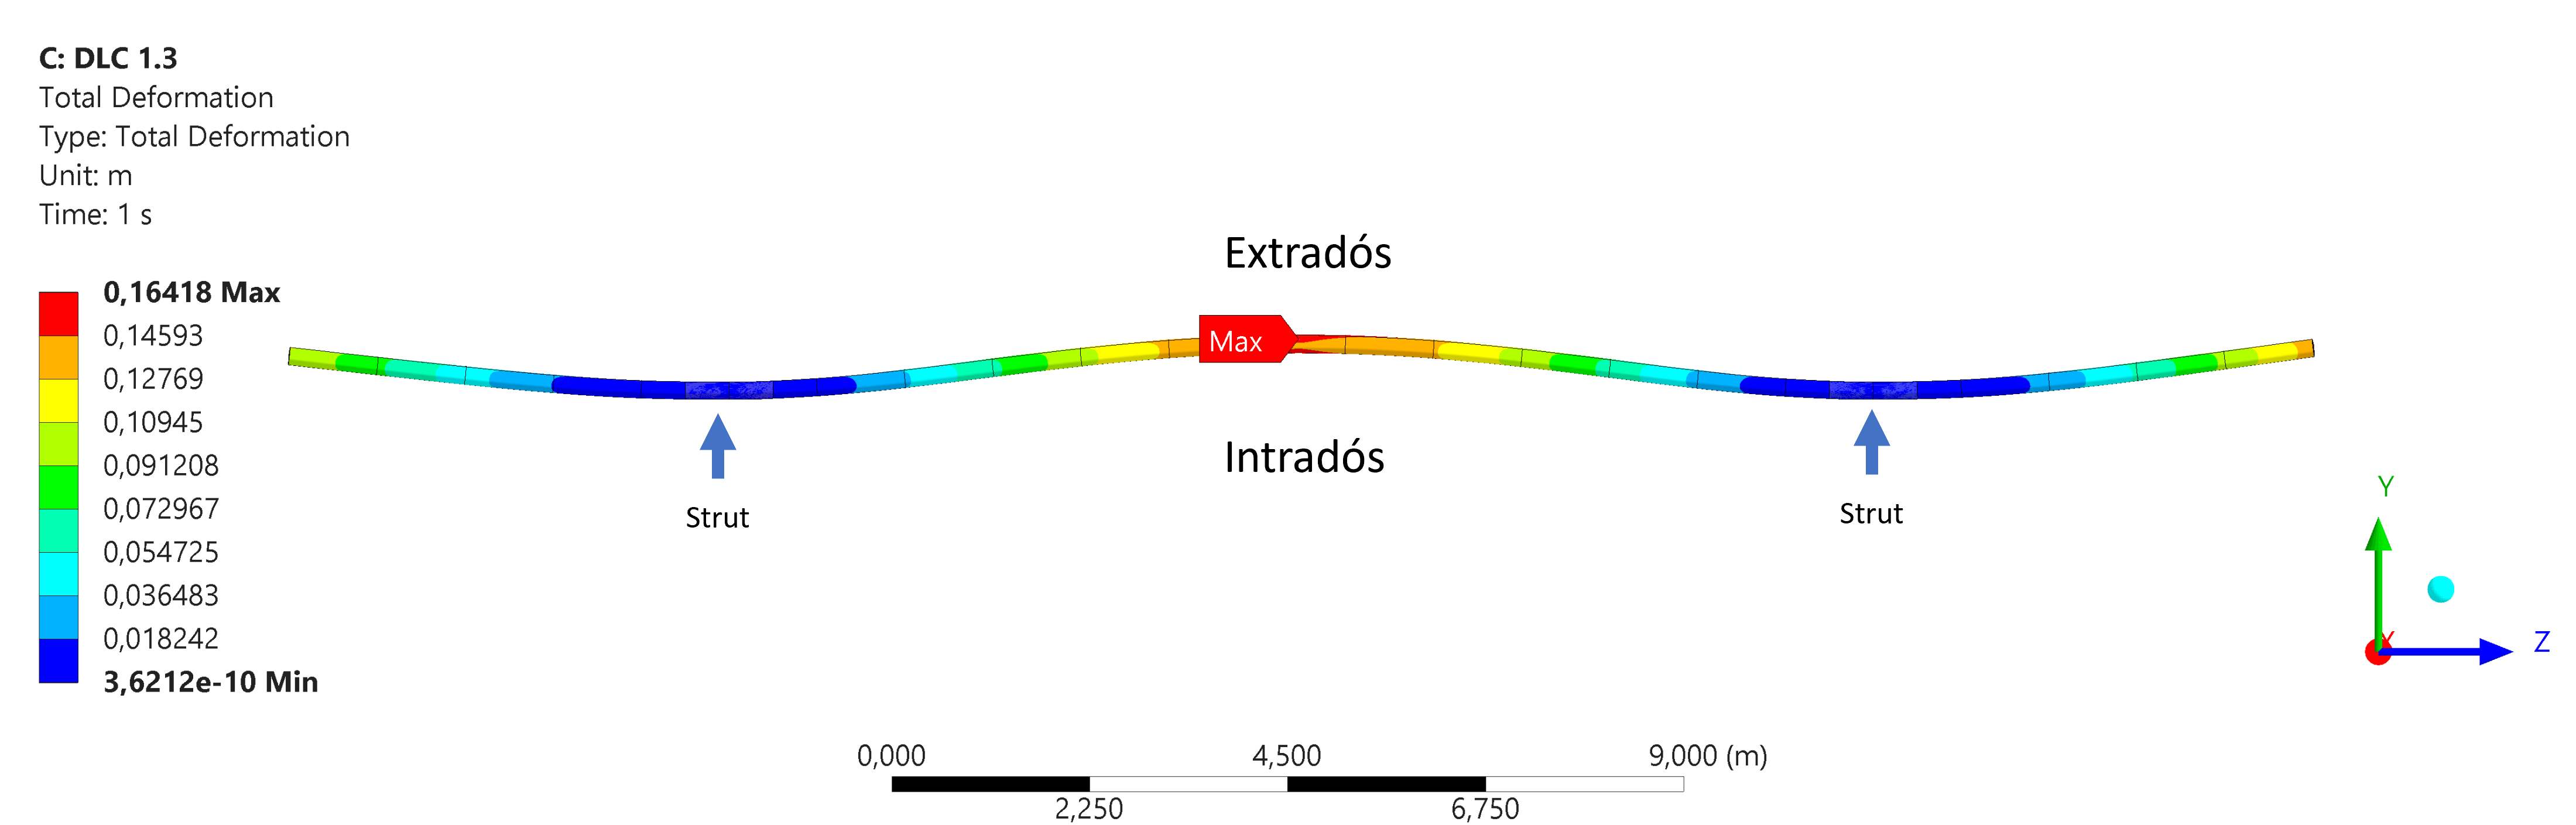
\includegraphics[width=\textwidth]{Figuras/Figuras Resultados/fem_deformacion13.png}
    \caption{Deformación total, DLC 1.3.}
    \label{fig:fem_deformacion13}
\end{figure}

Que la tensión máxima y la deformación resulten menores que en el DLC 1.1 pese a la mayor carga global tiene su origen en la distribución de las fuerzas. Ambos casos se resuelven con idénticas condiciones de borde y aceleraciones, por lo que la única diferencia entre ellos es el perfil de carga por estación. El DLC 1.1, extraído de un único instante de la simulación, concentra mayor carga en el vano central entre apoyos, cuya flexión solicita las conexiones y produce la flecha máxima del vano, mientras que el DLC 1.3, construido como media de máximos por estación, distribuye la carga de forma más suave hacia los voladizos (Sección~\ref{sec:comparacion_dlc}), lo que se refleja en una compresión levemente mayor pero una tracción y una deflexión menores.

\subsubsection{Contribución de las cargas inerciales}
\label{sec:solo_inercial}

Para cuantificar el peso de la rotación en el estado tensional, el modelo se resuelve adicionalmente con las cargas inerciales, aceleración centrífuga de $20{,}4\,g$ y gravedad, como única solicitación, sin fuerzas aerodinámicas. La tensión principal máxima resultante es $\sigma_{1,\max} = 114{,}5$~MPa en la misma zona crítica.

Este caso de referencia entrega una conclusión de diseño central, ya que la carga permanente de rotación produce por sí sola el $70\%$ de la tensión del caso gobernante ($114{,}5$ de $163{,}4$~MPa), mientras que el viento, incluso en su condición extrema de diseño a 50 años, aporta el $30\%$ restante. La pala está dimensionada principalmente por la fuerza centrífuga, es decir, por la decisión de control que fija la velocidad máxima de rotación en $42$~rpm, y no por el viento del emplazamiento. Este resultado también explica que las reacciones en los brazos apenas difieran entre ambos DLC, ya que la componente inercial, idéntica en los dos casos, domina el equilibrio global.

\subsubsection{Verificación de resistencia última}

La verificación de resistencia última emplea el criterio de máxima tensión principal, apropiado para materiales compuestos de matriz polimérica con comportamiento frágil~\parencite{Moraras2023}, según la Ec.~\ref{eq:criterio_uls}:

\begin{equation}
    \sigma_{1,\max} \leq \sigma_{u,d} = \frac{\sigma_u}{\gamma_m \cdot \gamma_n}
    \label{eq:criterio_uls}
\end{equation}

Con $\sigma_u = 242{,}1$~MPa, entregada por el fabricante de la pala (Tabla~\ref{tab:material_pala}), $\gamma_m = 1{,}30$ y $\gamma_n = 1{,}00$ según la Sección~\ref{sec:factores_seguridad}, la resistencia factoreada resulta según la Ec.~\ref{eq:sigma_ud_res}:

\begin{equation}
    \sigma_{u,d} = \frac{242{,}1}{1{,}30 \times 1{,}00} = 186{,}2\ \text{MPa}
    \label{eq:sigma_ud_res}
\end{equation}

Para el DLC 1.1, $\sigma_{1,\max} = 163{,}4$~MPa gobierna la verificación con un factor de reserva $\eta_{\text{ULS}}^{1.1} = 186{,}2 / 163{,}4 = 1{,}14$. Para el DLC 1.3, $\sigma_{1,\max} = 156{,}8$~MPa resulta en $\eta_{\text{ULS}}^{1.3} = 186{,}2 / 156{,}8 = 1{,}19$. Ambos casos satisfacen el criterio normativo, con márgenes del $14\%$ y el $19\%$ respectivamente.

En compresión, $\sigma_{3,\min} = -127{,}1$~MPa (DLC 1.1) y $-129{,}4$~MPa (DLC 1.3) se sitúan por debajo de la resistencia factoreada, por lo que esta verificación tampoco resulta condicionante en tensión; la relevancia de la compresión radica en la verificación de estabilidad que sigue.

\subsubsection{Verificación de estabilidad}

El análisis de pandeo lineal descrito en la Sección~\ref{sec:pandeo_met} se ejecuta sobre las soluciones estáticas de ambos casos de carga última. La Tabla~\ref{tab:pandeo} presenta los multiplicadores de carga de los tres primeros modos de cada caso.

\begin{table}[H]
    \centering
    \caption{Multiplicadores de carga del análisis de pandeo lineal.}
    \label{tab:pandeo}
    \begin{tabular}{ccc}
        \hline
        \textbf{Modo} & \textbf{$LM$, DLC 1.1} & \textbf{$LM$, DLC 1.3} \\
        \hline
        $1$ & $1{,}119$ & $1{,}131$ \\
        $2$ & $1{,}119$ & $1{,}131$ \\
        $3$ & $1{,}188$ & $1{,}167$ \\
        \hline
    \end{tabular}
\end{table}

Los modos corresponden a pandeo local de la piel de $8$~mm y se localizan en el vano central de la pala, en los paneles adyacentes al larguero, mecanismo característico de los cascarones de pared delgada de las palas de aerogenerador~\parencite{Boudounit2020}. El valor mínimo, $LM = 1{,}12$ (DLC 1.1), supera la unidad, por lo que el modelo no predice inestabilidad bajo la carga de diseño, pero no alcanza el umbral de $1{,}30$ de la Ec.~\ref{eq:criterio_pandeo}, por lo que la verificación de estabilidad no se satisface. Dado que el método lineal por autovalores constituye una cota superior de la carga crítica (Sección~\ref{sec:pandeo_met}), el margen faltante no es atribuible a conservadurismo del método.

Dos análisis de sensibilidad delimitan el origen del déficit. Primero, una configuración sin larguero interior resulta inviable, con multiplicadores inferiores a la unidad, lo que responde la pregunta de diseño planteada en la Sección~\ref{sec:material_pala}, ya que la omisión del larguero, alternativa que el fabricante evaluaba por facilidad de fabricación, no es estructuralmente viable con el espesor de piel estimado. Segundo, el aumento del espesor del larguero de $8$ a $12$~mm no modifica significativamente los multiplicadores, que se mantienen en torno a $1{,}1$. Este segundo resultado indica que el modo crítico está gobernado por los paneles de piel y no por el larguero. Una vez que este existe, seguir engrosándolo no aporta estabilidad, porque la capacidad de pandeo de un panel crece con el cuadrado de la razón entre su espesor y su ancho no apoyado (Ec.~\ref{eq:pandeo_placa}), y el larguero no modifica ninguna de las dos para los paneles adyacentes. En consecuencia, se mantiene el espesor de $8$~mm como configuración definitiva, y el cumplimiento del criterio de estabilidad queda supeditado a la rigidización de los paneles de piel, sea mediante elementos longitudinales adicionales (un segundo larguero o larguerillos), costillas transversales o un mayor espesor de piel en el vano central, alternativas cuya evaluación excede el alcance comprobatorio de este trabajo.

Que sea la estabilidad, y no la resistencia última, el criterio que no se satisface merece detenerse, porque no es el resultado que cabría anticipar. La razón es que ambos criterios interrogan propiedades distintas del laminado. La resistencia depende de cuánta tensión soporta el material, y en ella la pala conserva un factor de reserva de $1{,}14$; el pandeo depende de la rigidez del panel y de su geometría, y crece con el cuadrado de la razón entre el espesor de la piel y el ancho no apoyado (Ec.~\ref{eq:pandeo_placa}), de modo que un cascarón puede abollarse muy por debajo de la resistencia de su material.

Ese resultado señala, más que una deficiencia del diseño, el límite del modelo con que se lo evalúa, ya que tres de sus supuestos pesan directamente sobre él. El primero es el espesor de pared uniforme en todo el perímetro del perfil, adoptado al estimarlo desde la masa total de la pala (Sección~\ref{sec:material_pala}), cuando una distribución real concentraría material en las zonas de mayor solicitación y lo aligeraría en el resto. El segundo es la representación del laminado como un material isótropo equivalente, que no distingue la orientación del refuerzo, siendo que la carga crítica de un panel ortótropo depende de sus rigideces flexionales en cada dirección. El tercero es el propio larguero, cuyo espesor se igualó al del manto ante la falta de una definición del laminado. Los tres apuntan a que el margen obtenido debe leerse como una señal de que la sección requiere revisión, y no como una cuantificación exacta del déficit.

\subsubsection{Verificación de deflexiones}

La Sección 7.6.5 de la norma IEC 61400-1~\parencite{IEC61400-1} exige verificar que ninguna deflexión comprometa la integridad estructural ni produzca interferencia mecánica entre componentes. Para la configuración VAWT de palas rectas paralelas al eje de rotación, la deflexión radial no conlleva riesgo de impacto contra la torre. Las deflexiones máximas obtenidas del FEM bajo las cargas de diseño son $\delta_{\max} = 0{,}169$~m (DLC 1.1) y $0{,}164$~m (DLC 1.3), localizadas en el vano central entre apoyos. Referidas a la luz de dicho vano ($12$~m entre conexiones), representan una razón $\delta/L$ del $1{,}4\%$ en ambos casos. Estas deflexiones no comprometen la conexión con los struts ni el desempeño aerodinámico del rotor.

\subsection{Resumen de la verificación estructural}

La Tabla~\ref{tab:resumen_uls} sintetiza los resultados de la verificación a resistencia última para los DLC 1.1 y 1.3. La Tabla~\ref{tab:resumen_fatiga} presenta los resultados de la verificación a fatiga correspondiente al DLC 1.2.

\begin{table}[H]
    \centering
    \caption{Resumen de la verificación a fatiga.}
    \label{tab:resumen_fatiga}
    \begin{tabular}{llc}
        \hline
        \textbf{Símbolo} & \textbf{Descripción} & \textbf{DLC 1.2 (NTM)} \\
        \hline
        $\gamma_f$ & Factor parcial de carga & $1{,}00$ \\
        $\gamma_m \cdot \gamma_n$ & Factores parciales combinados & $1{,}96$ \\
        $\gamma_n$ & Factor de consecuencia (CC2, fatiga) & $1{,}15$ \\
        $K_{aero}$ & Factor de proporcionalidad momento-tensión & $0{,}752$~MPa/(kN$\cdot$m) \\
        $\sigma_{in}$ & Tensión media de origen inercial & $114{,}5$~MPa \\
        $D_{\text{año}}$ & Daño anual acumulado & $3{,}22 \times 10^{-9}$ \\
        $D_{20}$ & Daño acumulado en 20 años & $6{,}45 \times 10^{-8}$ \\
        \hline
    \end{tabular}
\end{table}

\begin{table}[H]
    \centering
    \caption{Resumen de la verificación a resistencia última.}
    \label{tab:resumen_uls}
    \begin{tabular}{llcc}
        \hline
        \textbf{Símbolo} & \textbf{Descripción} & \textbf{DLC 1.1 (NTM)} & \textbf{DLC 1.3 (ETM)} \\
        \hline
        \multicolumn{4}{c}{\textit{Cargas de diseño}} \\
        \hline
        $F_d$ & Carga de diseño global & $146{,}1$~kN & $152{,}1$~kN \\
        $F_{d,x}$ & Fuerza máx.\ por estación, eje $X_l$ & $6{,}78$~kN/m & $6{,}71$~kN/m \\
        $F_{d,y}$ & Fuerza máx.\ por estación, eje $Y_l$ & $2{,}40$~kN/m & $2{,}30$~kN/m \\
        $\gamma_f$ & Factor parcial de carga & $1{,}25$ & $1{,}35$ \\
        \hline
        \multicolumn{4}{c}{\textit{Tensiones (FEM)}} \\
        \hline
        $\sigma_{1,\max}$ & Tensión principal máxima & $163{,}4$~MPa & $156{,}8$~MPa \\
        $\sigma_{3,\min}$ & Tensión principal mínima & $-127{,}1$~MPa & $-129{,}4$~MPa \\
        \hline
        \multicolumn{4}{c}{\textit{Verificación del factor de seguridad}} \\
        \hline
        $\sigma_u/(\gamma_m \gamma_n)$ & Resistencia factoreada & $186{,}2$~MPa & $186{,}2$~MPa \\
        $\gamma_m$ & Factor parcial de material & $1{,}30$ & $1{,}30$ \\
        $\gamma_n$ & Factor de consecuencia de falla & $1{,}00$ & $1{,}00$ \\
        $\eta_{\text{ULS}}$ & Factor de reserva ($\sigma_u/(\gamma_m \gamma_n)/\sigma_{1,\max}$) & $1{,}14$ & $1{,}19$ \\
        \hline
        \multicolumn{4}{c}{\textit{Estabilidad (FEM)}} \\
        \hline
        $LM$ & Multiplicador de carga mínimo (modo 1) & $1{,}119$ & $1{,}131$ \\
        \hline
        \multicolumn{4}{c}{\textit{Deformación (FEM)}} \\
        \hline
        $\delta_{\max}$ & Deformación máxima & $0{,}169$~m & $0{,}164$~m \\
        --- & Ubicación & Centro & Centro \\
        \hline
    \end{tabular}
\end{table}

Los factores de reserva obtenidos ($\eta_{\text{ULS}} \geq 1{,}14$) y el daño acumulado por fatiga ($D_{20} = 6{,}45 \times 10^{-8} \ll 1{,}0$) confirman que la pala satisface los criterios normativos de resistencia última y fatiga establecidos en IEC 61400-1~\parencite{IEC61400-1}, y las deformaciones máximas se mantienen dentro de márgenes que no comprometen la operación del rotor. La verificación de estabilidad, en cambio, no se satisface, ya que el multiplicador de carga mínimo ($LM = 1{,}12 < 1{,}30$) muestra que el pandeo local de los paneles de piel gobierna el diseño. El caso de referencia con cargas exclusivamente inerciales cuantifica además que el $70\%$ de la tensión del caso gobernante proviene de la rotación, resultado que vincula el dimensionamiento estructural con la estrategia de control y que se desarrolla en el Capítulo~5.

\chapter{Conclusiones}

Este trabajo validó el diseño estructural de la pala de un aerogenerador offshore flotante de eje vertical mediante simulación aerodinámica en QBlade, conforme a los criterios de la norma IEC 61400-1~\parencite{IEC61400-1}. Las conclusiones se organizan en torno al cumplimiento de los objetivos planteados, las limitaciones del alcance y las líneas de trabajo que se abren a partir de los resultados obtenidos.

\section{Cumplimiento de los objetivos}

Respecto del primer objetivo específico, el comportamiento aerodinámico de la pala quedó caracterizado en la totalidad del rango operacional, y las 102 simulaciones LLFVW entregaron las series temporales de cargas que el objetivo exigía. Lo relevante para lo que sigue es que esas cargas llegan respaldadas, ya que cada eslabón de la cadena que las produce quedó contrastado con una referencia ajena al propio cálculo: las polares del NACA 0018 contra dos conjuntos de datos experimentales, el TSR óptimo del barrido DMST contra la solidez del rotor como parámetro puramente geométrico, y la curva de potencia resultante contra las turbinas H-rotor documentadas de escala comparable.

De ese objetivo se desprende también la velocidad máxima de rotación, que el fabricante no especifica y que se estimó en $42$~rpm. El valor resiste el contraste con las máquinas de referencia (Tabla~\ref{tab:comparacion_adim}), pero su consecuencia estructural no se hereda de ellas, ya que el menor radio del rotor en estudio eleva la aceleración centrífuga un $29\%$ sobre la de la T1-turbine en su propio límite de diseño. Siendo esta la solicitación que domina el estado tensional, conviene subrayar que se trata de un parámetro estimado, cuya confirmación queda pendiente de que la empresa libere el valor de diseño efectivo.

En cuanto al segundo objetivo, se desarrolló un modelo de elementos finitos de la pala con condiciones de borde y estados de carga equivalentes al escenario operacional, esto es, empotramiento en las conexiones con los struts, aceleración centrífuga de $20{,}4\,g$ mayorada por el factor parcial del caso, y fuerzas aerodinámicas de diseño aplicadas por estación conservando el signo del instante del que provienen. Dos análisis de convergencia de malla, uno sobre la tensión y otro sobre el autovalor de pandeo, acreditan que los resultados no dependen de la discretización.

De ese modelo se desprende una precaución para el diseño. La tensión máxima aparece en la zona de conexión con los brazos, que es también la que hubo que suponer ante la falta de un plano de la unión, de modo que el factor de reserva obtenido es sensible al detalle constructivo definitivo. Con un margen del $14\%$, ese detalle debe verificarse cuando se disponga de su geometría real.

El tercer objetivo se cumplió al verificar la integridad estructural bajo los tres casos de carga de producción de energía de la norma. La resistencia última se satisface con un factor de reserva de $1{,}26$, la deflexión no supera el $1{,}3\%$ de la luz entre conexiones y el daño por fatiga en 20 años, $D_{20} = 6{,}00 \times 10^{-3}$, queda por debajo del límite unitario con más de dos órdenes de magnitud de margen. La estabilidad, en cambio, no se cumple, y no por un margen estrecho, ya que el multiplicador de carga del primer modo vale $0{,}569$ frente al umbral de $1{,}20$ que la norma fija para el pandeo global de cascarones curvos. Falta un factor $2{,}11$, y al no alcanzar el multiplicador siquiera la unidad, el modelo predice inestabilidad bajo la propia carga de diseño. Es, con claridad, el criterio que gobierna el diseño.

Ese margen a fatiga merece una precisión. Por la planitud de la curva S-N del laminado, el daño escala con la amplitud de tensión elevada a $22{,}2$, de modo que los dos órdenes de magnitud de holgura sobre $D_{20}$ equivalen a un margen de apenas un $20\%$ sobre la tensión. La fatiga no es dimensionante, pero tampoco dispone del colchón que la cifra sugiere a primera vista, y su verificación queda condicionada a la precisión con que se calibre la relación entre momento y tensión en la sección crítica.

Que el criterio incumplido sea la estabilidad y no la resistencia última no es lo que cabría anticipar, y su explicación se desarrolla en la Sección~\ref{sec:resultados_fem}. De ella se desprende una conclusión con consecuencias para el diseño, y es que el margen de pandeo obtenido debe leerse como una señal de que la sección requiere revisión, y no como una cuantificación exacta del déficit, porque los supuestos del modelo sobre la distribución del espesor y sobre la orientación del refuerzo recaen precisamente sobre la magnitud que ese criterio evalúa.

Con los tres objetivos específicos cumplidos, el objetivo general queda alcanzado en su propósito de someter el diseño a la validación normativa. El resultado de esa validación es matizado, ya que la pala es válida en resistencia última, fatiga y deflexión bajo condiciones de funcionamiento nominal según IEC 61400-1, pero la verificación de estabilidad muestra que la configuración analizada, piel de $8$~mm con larguero interior del mismo espesor, queda por debajo del margen normativo de pandeo, por lo que la validez del diseño queda condicionada a la rigidización de los paneles de piel del vano central.

Del análisis se desprenden además tres conclusiones de diseño. Primero, el análisis de estabilidad responde la pregunta que planteaba el fabricante, que evaluaba omitir el larguero interior para facilitar la fabricación. La configuración sin larguero resulta claramente peor, por lo que el larguero es estructuralmente necesario; y dado que engrosarlo no mejora los multiplicadores, el cumplimiento del criterio exige rigidizar los paneles de piel del vano central. La comparación entre las dos vías disponibles es concluyente, ya que subdividir el panel más solicitado con un larguerillo longitudinal cuadruplica su capacidad por algo más de diez kilogramos, mientras que alcanzar el mismo resultado engrosando la piel exige del orden de cien. Segundo, las zonas que el diseño debe atender son distintas según el criterio, ya que la tensión máxima se localiza en las conexiones pala-brazo, lo que las señala como prioritarias para el detallamiento del laminado y las inspecciones en servicio, mientras que los modos críticos de pandeo se concentran en los paneles del vano central. Tercero, el diseño estructural de un rotor de eje vertical está gobernado por su velocidad máxima de giro, y este trabajo lo cuantifica, ya que la carga inercial permanente que impone la rotación produce por sí sola $114{,}5$~MPa, que son la mayor parte de la tensión del caso gobernante, frente a la fracción restante que aporta el viento en su condición extrema de diseño a 50 años. El dimensionamiento de la pala responde, por tanto, al valor que se fije para esa velocidad, $42$~rpm en este caso, equivalentes a $20{,}4\,g$ de aceleración centrífuga, y solo de forma secundaria al recurso eólico del emplazamiento. La consecuencia práctica es que fijar la velocidad máxima de giro es una decisión estructural antes que operacional, y que no puede resolverse mirando solo la curva de potencia.

En el plano metodológico, la comparación entre los DLC 1.1 y 1.3 deja una lección aplicable a cualquier verificación de este tipo. La Sección 7.4.2 de la norma IEC 61400-1~\parencite{IEC61400-1} permite omitir el análisis del DLC 1.1 cuando el DLC 1.3 lo envuelve, y ese envolvimiento no se produce aquí, ya que el DLC 1.3 gobierna en cuatro de las trece magnitudes evaluadas y en ninguna de las seis del apoyo superior, que es la sección más solicitada. Lo relevante es cómo se llega a esa conclusión. Si la comparación se hubiese resuelto sobre una única señal escalar, la fuerza total integrada sobre la pala, el DLC 1.3 la supera en un $5{,}4\%$ y el criterio habría autorizado prescindir precisamente del caso que gobierna. Evaluarlo magnitud a magnitud, sobre el conjunto de efectos de carga que la norma señala para la raíz de la pala, no es por tanto un refinamiento formal sino la diferencia entre acertar y equivocarse en la elección del caso de diseño. Que el ordenamiento obtenido coincida con el que \textcite{Galinos2015} reporta para otro rotor VAWT sugiere, además, que no se trata de una particularidad de esta máquina.

Una segunda lección metodológica proviene del sentido de la carga. El instante que maximiza el momento aerodinámico en la sección de apoyo resulta ser uno en que la fuerza normal apunta hacia el eje del rotor, de modo que se opone a la fuerza centrífuga en lugar de sumarse a ella. En una máquina donde la carga inercial domina la solicitación, el mayor extremo aerodinámico no produce el mayor estado tensional, y verificar solo ese instante habría dejado fuera la combinación realmente desfavorable. De ahí que cada componente del momento se extrapole en sus dos sentidos y que el modelo estructural reciba dos perfiles de carga por caso, uno por cada sentido de la componente normal. La advertencia es general para rotores de eje vertical, en los que la carga centrífuga es permanente y de signo fijo mientras la aerodinámica cambia de sentido a lo largo de cada revolución.

Una tercera observación atañe a la lectura del coeficiente de potencia. La definición convencional refiere la potencia media al cubo de la velocidad media del intervalo, supuesto válido con flujo uniforme y no con viento turbulento, donde la potencia disponible corresponde a la media del cubo de la velocidad. La diferencia no es menor a baja velocidad de viento, donde la intensidad de turbulencia relativa es mayor, y lleva a que el coeficiente así calculado alcance el límite de Betz sin que exista violación física alguna. Referido a la potencia que el campo transporta efectivamente, el máximo se sitúa en $0{,}503$ y se mantiene por debajo del límite en todo el rango. Cualquier comparación de rendimiento entre máquinas exige, por tanto, verificar antes sobre qué magnitud está definido el coeficiente que se compara.

El trabajo demuestra, además, que la metodología es replicable y de bajo costo de entrada, ya que la cadena completa, desde la caracterización del emplazamiento hasta la verificación por elementos finitos, se ejecutó con datos públicos chilenos y con QBlade, de código abierto, quedando Ansys como única herramienta comercial. Los contrastes independientes señalados más arriba son los que permiten sostener los resultados con la información disponible, pero no sustituyen a la medición. Si el proyecto avanza, la caracterización del emplazamiento debería respaldarse con una campaña de prospección eólica que mida in situ las condiciones de viento y turbulencia, ya que los parámetros que aquí se derivaron de reanálisis, entre ellos la velocidad media, la intensidad de turbulencia y la clase IEC del sitio, condicionan toda la cadena de cargas.

Esa campaña debería extenderse al estado de mar, que este trabajo no analizó por alcance. Su relevancia para las cargas de la pala no es la misma en todas las máquinas de esta familia. \textcite{Guo2018} simulan un H-rotor flotante bajo viento y oleaje combinados y encuentran que el movimiento de la plataforma amplifica las amplitudes de las fuerzas aerodinámicas hasta un $9{,}4\%$ en la componente normal y un $16{,}3\%$ en la tangencial respecto de la misma turbina sobre fundación fija, e incorpora a su contenido espectral la frecuencia del oleaje junto a la de paso de pala. \textcite{Borg2015} identifican la condición bajo la cual ese acoplamiento se vuelve crítico, ya que la excitación aerodinámica de una VAWT se concentra en su frecuencia de paso de pala, y en rotores muy grandes y de giro lento esa frecuencia cae dentro de la banda $0{,}5$--$0{,}9$~rad/s en que se concentra la energía del oleaje, con el consiguiente riesgo de excitación simultánea de origen aerodinámico e hidrodinámico.

Ese solapamiento no se produce en el rotor estudiado. Con tres palas girando a $42$~rpm, su frecuencia de paso de pala es de $13{,}2$~rad/s, más de un orden de magnitud por encima del extremo superior de esa banda, a diferencia del rotor de $5$~MW y giro lento que analizan \textcite{Borg2015}, cuya frecuencia de $0{,}77$~rad/s cae de lleno en ella. Cabe esperar, por tanto, que el oleaje incida sobre las cargas de la pala por la vía del movimiento de la plataforma, en el orden de magnitud que reporta \textcite{Guo2018}, y no por resonancia con la excitación del rotor. Comprobarlo exige el modelo acoplado que el alcance de este trabajo no incluyó.

\section{Limitaciones del alcance}

Los resultados deben interpretarse dentro del alcance definido al inicio del trabajo, que estableció el análisis bajo condiciones nominales de operación. Por ello se evaluaron los casos de producción de energía DLC 1.1, 1.2 y 1.3, quedando fuera del estudio las situaciones de arranque, parada, falla del sistema de control y condiciones de reposo, que la norma contempla en otros casos de carga. Esta delimitación es consistente con la evidencia de que en una VAWT la operación normal con turbulencia gobierna las cargas en la raíz de la pala~\parencite{Galinos2016,Sutherland2012}, pero no la convierte en una condición suficiente, ya que trabajos recientes sobre H-rotores rígidos y sobre plataformas flotantes han identificado contribuciones no despreciables en casos habitualmente descartados, en particular el rotor detenido bajo viento extremo~\parencite{Moore2024,Sakib2022}. Verificar la pala frente a ese conjunto completo excede el alcance comprometido y se plantea como extensión del estudio.

Dentro de ese marco, la verificación de la velocidad máxima de rotación adoptada ($42$~rpm) es estructural, esto es, acredita que la pala resiste las cargas centrífugas y aerodinámicas asociadas, pero no incluye el análisis modal del rotor ni la comprobación de resonancia entre la frecuencia de paso de pala y los modos propios de la estructura. Dicha verificación excede el dominio de cálculo definido, que comprende únicamente la pala, y requiere las propiedades de los brazos, la torre y la plataforma. La experiencia documentada muestra que ese criterio no es accesorio, ya que en las máquinas construidas es la estructura, y no la aerodinámica, la que termina fijando la velocidad máxima de giro. En el prototipo de Sandia, el cruce de la frecuencia de paso de pala con el primer modo de torre en el plano acotó la velocidad máxima practicable a $38$~rpm~\parencite{Sutherland2012}, y en la T1-turbine el límite operacional se redujo de $33$ a $22$~rpm tras la instalación de los tensores de la torre, también por resonancia~\parencite{Mollerstrom2017}. Su comprobación constituye, por tanto, un requisito previo a la adopción definitiva de las $42$~rpm.

Conviene explicitar, en relación con lo anterior, que la velocidad máxima de rotación se trató aquí como un dato de entrada y no como una variable de diseño. El valor se fijó a partir del criterio aerodinámico, aplicando el TSR de diseño a la velocidad de viento nominal, y sobre él se verificó la pala en un único sentido, sin iterar entre la velocidad adoptada y el dimensionamiento resultante. Esa decisión responde al alcance comprometido, que es verificar una configuración dada y no optimizarla, pero sobre todo a la información disponible, ya que el espesor de pared no proviene del fabricante sino que se estimó a partir de la masa total de la pala. Iterar espesores sobre una magnitud que es en sí misma un supuesto habría entregado un óptimo aparente, no un diseño mejor. Los resultados respaldan además que la velocidad de giro es el parámetro estructuralmente decisivo, ya que la carga inercial que impone aporta el $70\%$ de la tensión del caso gobernante, de modo que una eventual iteración entre velocidad de rotación y dimensionamiento de la sección es una línea pertinente, condicionada a disponer de la definición del laminado y del modelo modal del rotor completo.

La influencia del oleaje y de la dinámica acoplada entre el rotor y la plataforma tampoco se consideró, ya que su modelación requiere información de la plataforma flotante y de los sistemas de fondeo con la que no se cuenta. El desarrollo de este trabajo coincidió con la fase de aprobación de presupuesto del proyecto, por lo que parte de la información de diseño aún no estaba disponible al término de la práctica; las condiciones no especificadas, entre ellas la velocidad máxima de rotación, el exponente de fatiga del laminado y el espesor de pared uniforme, se asumieron a partir de los datos públicos del fabricante y de valores documentados en la literatura, dejando cada supuesto declarado explícitamente en la metodología. Que los resultados aerodinámicos y estructurales resultaran consistentes con la evidencia experimental y con turbinas de escala comparable respalda la razonabilidad de estos supuestos.

Por último, el modelo estructural representa el laminado mediante el conjunto isótropo equivalente declarado en la Sección~\ref{sec:material_pala}, idealización cuyo alcance ya se discutió al comentar el resultado de estabilidad y que afecta sobre todo a esa verificación.

\section{Trabajo futuro}

De las limitaciones anteriores se desprenden extensiones naturales del estudio. Cuando el proyecto disponga de los parámetros reales de funcionamiento de la turbina, esto es, la velocidad máxima de rotación de diseño, el laminado definitivo y la distribución de espesores, el análisis puede repetirse refinando los supuestos, con la ventaja de que la cadena de cálculo ya está construida y validada.

Una extensión de menor coste y de efecto inmediato sobre la confianza en los resultados es ampliar el número de realizaciones por velocidad en la banda alta. La Sección G.4.1 del Anexo G pide al menos quince realizaciones por velocidad entre $V_r - 2$~m/s y la velocidad de corte, frente a las seis con que se ejecutó esta campaña~\parencite{IEC61400-1}. Son precisamente las velocidades que dominan la cola de la extrapolación y la práctica totalidad del daño por fatiga, de modo que el refuerzo del muestreo ahí reduce la incertidumbre donde más pesa, con un costo de cómputo acotado a siete velocidades.

Un refinamiento adicional del modelo estructural consiste en simular el laminado capa por capa mediante el módulo ACP de Ansys, en lugar de evaluar el compuesto como material homogéneo, lo que permitiría identificar el modo de falla de la fibra y capturar la ortotropía que condiciona tanto la resistencia como la carga crítica de pandeo. Con un margen en tensión del $14\%$ y una verificación de estabilidad no satisfecha, ese nivel de detalle gana relevancia. La herramienta es conocida y su aplicación quedó supeditada únicamente a disponer de la definición del laminado.

En el plano de la estabilidad, el incumplimiento de la verificación de pandeo define la extensión prioritaria y orienta el rediseño de la sección. El margen disponible en fatiga indica que el material no está limitado por la acumulación de daño, de modo que todo refuerzo adicional debe destinarse a rigidizar los paneles de piel del vano central, cuya capacidad gobierna el modo crítico una vez incorporado el larguero: un segundo larguero, larguerillos longitudinales, costillas transversales o un mayor espesor local. Sobre la configuración corregida corresponde repetir la cadena de verificación completa, dado que cualquier rigidización modifica la masa, la rigidez y la distribución de tensiones, y complementarla con un análisis de pandeo no lineal que incorpore imperfecciones geométricas, pues el método lineal por autovalores entrega una cota superior de la carga crítica.

Junto a lo anterior, el análisis modal del rotor completo permitiría verificar que la velocidad de rotación adoptada no induzca resonancia, condición que en la turbina de referencia obligó a reducir el límite operacional. A ello se suma someter la pala a los restantes casos de carga de IEC 61400-1, en particular los eventos transitorios de arranque y parada y las condiciones extremas con rotor detenido, y la incorporación del oleaje y de la dinámica acoplada entre el rotor y la plataforma, una vez disponible la información del sistema de flotación, que permitiría verificar la pala en el entorno offshore completo.

Todas estas extensiones comparten una condición favorable: la cadena de análisis quedó construida, contrastada en cada etapa y documentada, de modo que incorporarlas constituye un refinamiento y no una reconstrucción. El trabajo cierra con dos resultados de distinta naturaleza. Por una parte, un procedimiento de verificación estructural completo, que abarca desde la caracterización del emplazamiento hasta el modelo de elementos finitos y resulta aplicable a otras palas de configuración similar. Por otra, un diagnóstico de la pala analizada, en el que la resistencia última, la fatiga y las deflexiones quedan verificadas, mientras que la estabilidad de los paneles de piel constituye la condición pendiente para considerar el diseño apto para fabricación.


\newpage
\chapter*{Declaración de uso de inteligencia artificial}
\addcontentsline{toc}{chapter}{Declaración de uso de inteligencia artificial}
\label{sec:declaracion_ia}

En la elaboración de este trabajo se utilizaron herramientas de inteligencia artificial generativa (Claude, de Anthropic) como apoyo en tareas de redacción y de programación. Su uso se concentró en tres áreas: la edición de estilo y la revisión de coherencia interna del texto, la verificación de consistencia entre los valores reportados en los distintos capítulos, y la asistencia en la escritura de los scripts de Python empleados para el post-proceso de las series temporales de carga (ajuste de Weibull, extrapolación de Gumbel a 50 años, conteo Rainflow y regla de Palmgren-Miner) y para la generación de figuras.

Las herramientas no se emplearon para generar datos, resultados ni conclusiones. La caracterización del emplazamiento, la construcción del modelo aerodinámico y las simulaciones en QBlade, el modelo de elementos finitos en Ansys y la interpretación de los resultados corresponden íntegramente al autor. Los algoritmos de post-proceso asistidos por estas herramientas fueron verificados de forma independiente contra los procedimientos descritos en los anexos F y G de la norma IEC 61400-1.

El autor revisó y validó la totalidad del contenido del documento, y asume la responsabilidad plena sobre los datos, los argumentos y las conclusiones presentados.


\newpage
\printnoidxglossary[type=\acronymtype, title={Glosario}, sort=word, nonumberlist]

\glsaddall
\begin{singlespace}
\printnoidxglossary[type=simbolos, title={Nomenclatura}, sort=word, nogroupskip, style=nomenclatura]
\end{singlespace}

\newpage
\begin{singlespace}
\printbibliography[heading=bibintoc, title={Bibliografía}]
\end{singlespace}

\chapter*{Anexo A}
\addcontentsline{toc}{chapter}{Anexo A: Fuerzas de diseño por estación}

\setcounter{table}{0}
\renewcommand{\thetable}{A.\arabic{table}}
\setcounter{figure}{0}
\renewcommand{\thefigure}{A.\arabic{figure}}

\section*{Fuerzas de diseño por estación para ingreso al modelo FEM}
\label{anexo:fuerzas}

Las tablas de este anexo entregan, para cada una de las $21$ estaciones de la pala, la
fuerza aerodinámica que la simulación registra y la fuerza puntual con que esa estación
se carga en el modelo de elementos finitos. Se presentan cuatro tablas, una por cada
combinación de caso de carga último y sentido de la componente normal, según se explica
en la Sección~\ref{sec:comparacion_dlc}.

Las columnas se interpretan como sigue.

\begin{itemize}
    \item \textbf{Est.} numera las estaciones desde la base de la pala hacia su extremo
          superior, y \textbf{z} es la cota del centroide de cada una sobre la base, que
          es el punto en que la carga remota debe aplicarse en el modelo.
    \item \textbf{$\Delta s$} es la longitud de pala que representa la estación. Los
          $21$ valores suman por construcción los $23{,}000$~m de envergadura.
    \item \textbf{$F_{sim,n}$} y \textbf{$F_{sim,t}$} son la fuerza aerodinámica por
          unidad de longitud que entrega la simulación, en N/m.
    \item \textbf{$F_{d,n}$} y \textbf{$F_{d,t}$} son la fuerza puntual de diseño, en N,
          que resulta de multiplicar la anterior por $\Delta s$ y por el factor de
          escalamiento del caso.
\end{itemize}

Los valores conservan su signo, y el signo es el que fija el sistema local de la pala de
la Figura~\ref{fig:ejes_locales}, determinado por medición en la
Sección~\ref{sec:ejes_locales_res}. La componente normal $F_n$ es \textbf{positiva hacia
el eje del rotor} y negativa hacia afuera, esto es, en el sentido de la fuerza
centrífuga. La componente tangencial $F_t$ es \textbf{positiva en el sentido del
movimiento de la pala}, que en un H-rotor apunta hacia el borde de ataque. Respetar
ambos signos al ingresar las cargas es indispensable, ya que de ellos depende si la
solicitación aerodinámica se suma o se resta a la inercial.

\begin{table}[H]
    \centering
    \caption{Fuerzas por estación para el DLC 1.1, carga normal hacia el eje del rotor.}
    \label{tab:anexo_fuerzas_dlc11}
    \begin{tabular}{ccrrrrr}
        \hline
        \textbf{Est.} & $\mathbf{z}$ [m] & $\mathbf{\Delta s}$ [m] & $\mathbf{F_{sim,n}}$ [N/m] & $\mathbf{F_{sim,t}}$ [N/m] & $\mathbf{F_{d,n}}$ [N] & $\mathbf{F_{d,t}}$ [N] \\
        \hline
        1 & 0{,}064 & 0{,}1284 & 821 & 34 & 158 & 6 \\
        2 & 0{,}320 & 0{,}3825 & 2556 & 380 & 1461 & 217 \\
        3 & 0{,}825 & 0{,}6279 & 3217 & 587 & 3019 & 551 \\
        4 & 1{,}569 & 0{,}8594 & 3604 & 727 & 4628 & 934 \\
        5 & 2{,}534 & 1{,}0716 & 3691 & 732 & 5911 & 1172 \\
        6 & 3{,}700 & 1{,}2600 & 3783 & 740 & 7124 & 1393 \\
        7 & 5{,}040 & 1{,}4201 & 3863 & 757 & 8198 & 1606 \\
        8 & 6{,}524 & 1{,}5486 & 3853 & 760 & 8916 & 1760 \\
        9 & 8{,}120 & 1{,}6424 & 3825 & 762 & 9388 & 1871 \\
        10 & 9{,}791 & 1{,}6996 & 3911 & 798 & 9935 & 2027 \\
        11 & 11{,}500 & 1{,}7188 & 4205 & 942 & 10801 & 2421 \\
        12 & 13{,}209 & 1{,}6996 & 4520 & 1050 & 11480 & 2667 \\
        13 & 14{,}880 & 1{,}6424 & 5118 & 1361 & 12563 & 3340 \\
        14 & 16{,}476 & 1{,}5486 & 5641 & 1668 & 13055 & 3860 \\
        15 & 17{,}960 & 1{,}4201 & 5940 & 1448 & 12605 & 3072 \\
        16 & 19{,}300 & 1{,}2600 & 6021 & 1754 & 11336 & 3303 \\
        17 & 20{,}466 & 1{,}0716 & 6059 & 1760 & 9703 & 2819 \\
        18 & 21{,}431 & 0{,}8594 & 5677 & 1544 & 7291 & 1983 \\
        19 & 22{,}175 & 0{,}6279 & 5223 & 1292 & 4902 & 1212 \\
        20 & 22{,}680 & 0{,}3825 & 4615 & 1008 & 2638 & 576 \\
        21 & 22{,}936 & 0{,}1284 & 2032 & 201 & 390 & 39 \\
        \hline
    \end{tabular}
\end{table}

\begin{table}[H]
    \centering
    \caption{Fuerzas por estación para el DLC 1.1, carga normal hacia afuera.}
    \label{tab:anexo_fuerzas_dlc11_ext}
    \begin{tabular}{ccrrrrr}
        \hline
        \textbf{Est.} & $\mathbf{z}$ [m] & $\mathbf{\Delta s}$ [m] & $\mathbf{F_{sim,n}}$ [N/m] & $\mathbf{F_{sim,t}}$ [N/m] & $\mathbf{F_{d,n}}$ [N] & $\mathbf{F_{d,t}}$ [N] \\
        \hline
        1 & 0{,}064 & 0{,}1284 & $-$328 & $-$26 & $-$60 & $-$5 \\
        2 & 0{,}320 & 0{,}3825 & $-$1591 & 58 & $-$873 & 32 \\
        3 & 0{,}825 & 0{,}6279 & $-$2008 & 119 & $-$1809 & 107 \\
        4 & 1{,}569 & 0{,}8594 & $-$2183 & 147 & $-$2693 & 182 \\
        5 & 2{,}534 & 1{,}0716 & $-$2112 & 118 & $-$3249 & 182 \\
        6 & 3{,}700 & 1{,}2600 & $-$1919 & 77 & $-$3471 & 140 \\
        7 & 5{,}040 & 1{,}4201 & $-$1871 & 64 & $-$3812 & 131 \\
        8 & 6{,}524 & 1{,}5486 & $-$2134 & 101 & $-$4742 & 224 \\
        9 & 8{,}120 & 1{,}6424 & $-$2216 & 126 & $-$5224 & 296 \\
        10 & 9{,}791 & 1{,}6996 & $-$2595 & 196 & $-$6331 & 477 \\
        11 & 11{,}500 & 1{,}7188 & $-$3199 & 317 & $-$7891 & 782 \\
        12 & 13{,}209 & 1{,}6996 & $-$3373 & 335 & $-$8228 & 817 \\
        13 & 14{,}880 & 1{,}6424 & $-$3709 & 418 & $-$8741 & 986 \\
        14 & 16{,}476 & 1{,}5486 & $-$4239 & 573 & $-$9421 & 1273 \\
        15 & 17{,}960 & 1{,}4201 & $-$4885 & 811 & $-$9957 & 1653 \\
        16 & 19{,}300 & 1{,}2600 & $-$5122 & 920 & $-$9262 & 1664 \\
        17 & 20{,}466 & 1{,}0716 & $-$5156 & 928 & $-$7929 & 1427 \\
        18 & 21{,}431 & 0{,}8594 & $-$4762 & 752 & $-$5873 & 927 \\
        19 & 22{,}175 & 0{,}6279 & $-$4148 & 530 & $-$3738 & 477 \\
        20 & 22{,}680 & 0{,}3825 & $-$3407 & 328 & $-$1870 & 180 \\
        21 & 22{,}936 & 0{,}1284 & $-$1430 & 12 & $-$264 & 2 \\
        \hline
    \end{tabular}
\end{table}

\begin{table}[H]
    \centering
    \caption{Fuerzas por estación para el DLC 1.3, carga normal hacia el eje del rotor.}
    \label{tab:anexo_fuerzas_dlc13}
    \begin{tabular}{ccrrrrr}
        \hline
        \textbf{Est.} & $\mathbf{z}$ [m] & $\mathbf{\Delta s}$ [m] & $\mathbf{F_{sim,n}}$ [N/m] & $\mathbf{F_{sim,t}}$ [N/m] & $\mathbf{F_{d,n}}$ [N] & $\mathbf{F_{d,t}}$ [N] \\
        \hline
        1 & 0{,}064 & 0{,}1284 & 890 & 41 & 154 & 7 \\
        2 & 0{,}320 & 0{,}3825 & 2739 & 441 & 1414 & 228 \\
        3 & 0{,}825 & 0{,}6279 & 3280 & 614 & 2781 & 521 \\
        4 & 1{,}569 & 0{,}8594 & 3545 & 706 & 4113 & 819 \\
        5 & 2{,}534 & 1{,}0716 & 3858 & 817 & 5582 & 1182 \\
        6 & 3{,}700 & 1{,}2600 & 3995 & 859 & 6796 & 1460 \\
        7 & 5{,}040 & 1{,}4201 & 4108 & 929 & 7876 & 1780 \\
        8 & 6{,}524 & 1{,}5486 & 4114 & 888 & 8600 & 1855 \\
        9 & 8{,}120 & 1{,}6424 & 3956 & 862 & 8773 & 1910 \\
        10 & 9{,}791 & 1{,}6996 & 4180 & 958 & 9592 & 2199 \\
        11 & 11{,}500 & 1{,}7188 & 4115 & 947 & 9547 & 2196 \\
        12 & 13{,}209 & 1{,}6996 & 4601 & 1133 & 10556 & 2600 \\
        13 & 14{,}880 & 1{,}6424 & 4727 & 1195 & 10481 & 2650 \\
        14 & 16{,}476 & 1{,}5486 & 4924 & 1229 & 10294 & 2570 \\
        15 & 17{,}960 & 1{,}4201 & 5196 & 1346 & 9962 & 2581 \\
        16 & 19{,}300 & 1{,}2600 & 5501 & 1523 & 9356 & 2591 \\
        17 & 20{,}466 & 1{,}0716 & 5750 & 1545 & 8319 & 2236 \\
        18 & 21{,}431 & 0{,}8594 & 5757 & 1674 & 6679 & 1943 \\
        19 & 22{,}175 & 0{,}6279 & 5485 & 1508 & 4650 & 1279 \\
        20 & 22{,}680 & 0{,}3825 & 4809 & 1141 & 2483 & 589 \\
        21 & 22{,}936 & 0{,}1284 & 2213 & 248 & 384 & 43 \\
        \hline
    \end{tabular}
\end{table}

\begin{table}[H]
    \centering
    \caption{Fuerzas por estación para el DLC 1.3, carga normal hacia afuera.}
    \label{tab:anexo_fuerzas_dlc13_ext}
    \begin{tabular}{ccrrrrr}
        \hline
        \textbf{Est.} & $\mathbf{z}$ [m] & $\mathbf{\Delta s}$ [m] & $\mathbf{F_{sim,n}}$ [N/m] & $\mathbf{F_{sim,t}}$ [N/m] & $\mathbf{F_{d,n}}$ [N] & $\mathbf{F_{d,t}}$ [N] \\
        \hline
        1 & 0{,}064 & 0{,}1284 & $-$428 & $-$25 & $-$74 & $-$4 \\
        2 & 0{,}320 & 0{,}3825 & $-$1939 & 110 & $-$1001 & 57 \\
        3 & 0{,}825 & 0{,}6279 & $-$2466 & 207 & $-$2091 & 175 \\
        4 & 1{,}569 & 0{,}8594 & $-$2778 & 277 & $-$3223 & 322 \\
        5 & 2{,}534 & 1{,}0716 & $-$3111 & 359 & $-$4501 & 520 \\
        6 & 3{,}700 & 1{,}2600 & $-$3246 & 384 & $-$5522 & 653 \\
        7 & 5{,}040 & 1{,}4201 & $-$3245 & 375 & $-$6222 & 719 \\
        8 & 6{,}524 & 1{,}5486 & $-$3306 & 393 & $-$6912 & 821 \\
        9 & 8{,}120 & 1{,}6424 & $-$3448 & 450 & $-$7646 & 998 \\
        10 & 9{,}791 & 1{,}6996 & $-$3391 & 431 & $-$7781 & 990 \\
        11 & 11{,}500 & 1{,}7188 & $-$3566 & 495 & $-$8275 & 1148 \\
        12 & 13{,}209 & 1{,}6996 & $-$3870 & 561 & $-$8879 & 1287 \\
        13 & 14{,}880 & 1{,}6424 & $-$3931 & 564 & $-$8715 & 1249 \\
        14 & 16{,}476 & 1{,}5486 & $-$4049 & 584 & $-$8464 & 1222 \\
        15 & 17{,}960 & 1{,}4201 & $-$4293 & 678 & $-$8230 & 1301 \\
        16 & 19{,}300 & 1{,}2600 & $-$4485 & 775 & $-$7629 & 1319 \\
        17 & 20{,}466 & 1{,}0716 & $-$4685 & 851 & $-$6778 & 1232 \\
        18 & 21{,}431 & 0{,}8594 & $-$4742 & 838 & $-$5501 & 973 \\
        19 & 22{,}175 & 0{,}6279 & $-$4346 & 661 & $-$3684 & 561 \\
        20 & 22{,}680 & 0{,}3825 & $-$3594 & 402 & $-$1856 & 207 \\
        21 & 22{,}936 & 0{,}1284 & $-$1552 & 27 & $-$269 & 5 \\
        \hline
    \end{tabular}
\end{table}


\chapter*{Anexo B}
\addcontentsline{toc}{chapter}{Anexo B: Procesamiento de cargas del DLC 1.1}

\setcounter{table}{0}
\renewcommand{\thetable}{B.\arabic{table}}
\setcounter{figure}{0}
\renewcommand{\thefigure}{B.\arabic{figure}}

\section*{Procesamiento de cargas del DLC 1.1: extrapolación al período de retorno de 50 años}
\label{anexo:dlc11}

Este anexo reproduce el código que transforma las series temporales entregadas por QBlade en las cargas de diseño del DLC 1.1, siguiendo el procedimiento del Anexo G de IEC 61400-1~\parencite{IEC61400-1} descrito en la Sección~\ref{sec:anexo_f}. Se omiten las rutinas de exportación a planilla y de generación de figuras, por no formar parte del cálculo. El procesamiento parte de $72$ realizaciones, correspondientes a $12$ velocidades de viento y $6$ semillas de turbulencia cada una.

\subsection*{Geometría y parámetros de entrada}

La pala se discretiza en los mismos $21$ paneles de reparto coseno con que se resuelve la aerodinámica, de modo que la carga se lee donde el método calcula efectivamente la circulación (Sección~\ref{sec:discretizacion}).

\begin{pycode}
# -*- coding: utf-8 -*-
"""
DLC 1.1 - Extrapolación de cargas extremas según el Anexo G de IEC 61400-1.
Entrada : 72 series temporales de fuerzas por estación (12 V x 6 semillas).
Salida  : carga característica F_k a 50 años y carga de diseño F_d de cada
          una de las trece magnitudes, y el perfil espacial de diseño.
"""
import csv, glob, json, math, os, re
from collections import defaultdict
import numpy as np

# --- Geometría de la pala y discretización ------------------------------
# Los bordes de panel siguen el reparto coseno, que concentra estaciones
# hacia los extremos, donde los gradientes de circulación son mayores. Los
# anchos suman por construcción la envergadura exacta, de modo que la
# integración espacial no introduce error de cierre.
ENVERGADURA = 23.0
N_PAN   = 21
BORDES  = 0.5 * ENVERGADURA * (1.0 - np.cos(np.linspace(0.0, np.pi, N_PAN + 1)))
Z_PAN   = 0.5 * (BORDES[:-1] + BORDES[1:])   # centro de panel [m]
DELTA_S = np.diff(BORDES)                    # ancho de panel [m]

# Secciones de apoyo: las dos conexiones con los brazos, que son la "raíz"
# de la pala en el sentido de la Sección 3.1 de IEC 61400-5.
Z_APOYO_INF = 5.0
Z_APOYO_SUP = 18.0

# Direcciones de la envolvente. IEC 61400-5 6.1.4.3 da por suficiente un
# conjunto repartido uniformemente en al menos doce direcciones.
N_DIRECCIONES = 12

# --- Parámetros normativos ----------------------------------------------
T_DISCARD = 50.0                       # tramo inicial descartado [s]. La
                                       # norma exige eliminar al menos los
                                       # 5 s iniciales, o mas si es
                                       # necesario (Seccion 7.5).
T_OBS     = 600.0                      # ventana útil de cada realización [s]
T_RETURN  = 50 * 365.25 * 24 * 3600.0  # período de retorno de 50 años [s]

# Probabilidad de excedencia objetivo. La Sección 7.6.2.2 de la norma
# declara ese mismo valor, 3,8e-7, como el máximo admisible.
PE_TARGET = T_OBS / T_RETURN

# Factor parcial de carga. La norma admite reducirlo de 1,35 a 1,25 para
# el DLC 1.1 cuando la carga se obtiene por extrapolación estadística
# según el Anexo G (Sección 7.6.2.2, nota a de la Tabla 3).
GAMMA_F = 1.25
\end{pycode}

\subsection*{Efectos de carga que se extrapolan}

QBlade entrega, en cada paso de tiempo, la fuerza por unidad de longitud en las $21$ estaciones y en las dos direcciones del sistema local de la pala contenidas en el plano del perfil. De ese vector se derivan los efectos de carga sobre los que opera la extrapolación, que son los momentos flectores en las dos secciones de apoyo.

\begin{pycode}
def fuerzas_puntuales(fn_lin, ft_lin):
    """Pasa de fuerza por unidad de longitud [N/m] a fuerza de panel [N]."""
    return fn_lin * DELTA_S, ft_lin * DELTA_S


def momentos_en_apoyo(fn_lin, ft_lin, z_c, lado):
    """
    Momento flector en una sección de apoyo, producido por el voladizo que
    esa sección sostiene.

    Cortando en el apoyo y sumando solo el voladizo libre, el resultado
    queda estáticamente determinado y no depende de las condiciones de
    contorno. El vano central entre apoyos no lo está, y por eso se
    resuelve en el modelo de elementos finitos y no aquí.

    Devuelve (m_x, m_y): m_x lo genera la componente tangencial y flecta
    en torno al eje local X; m_y lo genera la normal y flecta en torno a Y.
    """
    fn, ft = fuerzas_puntuales(fn_lin, ft_lin)
    if lado == 'inf':
        sel   = Z_PAN < z_c
        brazo = z_c - Z_PAN[sel]
    else:
        sel   = Z_PAN > z_c
        brazo = Z_PAN[sel] - z_c
    m_x = (ft[..., sel] * brazo).sum(axis=-1)
    m_y = (fn[..., sel] * brazo).sum(axis=-1)
    return m_x, m_y


def envolvente_direccional(m_x, m_y, n=N_DIRECCIONES):
    """
    Máximo del momento proyectado sobre n direcciones repartidas
    uniformemente en la sección (IEC 61400-5 6.1.4.3, enfoque avanzado).

    Al recorrer las n direcciones el círculo completo, la proyección cubre
    los dos sentidos de cada componente y no hace falta tomar valor
    absoluto. Por construcción el resultado nunca supera el módulo del
    vector, y solo lo iguala cuando este apunta a una de las direcciones.
    """
    th   = np.linspace(0.0, 2.0 * math.pi, n, endpoint=False)
    proy = (np.outer(np.atleast_1d(m_x), np.cos(th))
            + np.outer(np.atleast_1d(m_y), np.sin(th)))
    return proy.max(axis=1)


def f_total(fn_lin, ft_lin):
    """Fuerza total integrada sobre la envergadura, en norma euclídea."""
    fn, ft = fuerzas_puntuales(fn_lin, ft_lin)
    return np.hypot(fn, ft).sum(axis=-1)


def efectos_de_carga(fn_lin, ft_lin):
    """Las trece magnitudes que se extrapolan, para una serie completa."""
    mx_i, my_i = momentos_en_apoyo(fn_lin, ft_lin, Z_APOYO_INF, 'inf')
    mx_s, my_s = momentos_en_apoyo(fn_lin, ft_lin, Z_APOYO_SUP, 'sup')
    return {
        # Componentes con signo, en sus dos sentidos: el extremo de diseño
        # de una magnitud predominantemente negativa está en su mínimo, y
        # la norma pide los valores extremos, que son ambos.
        'M_x_apoyo_inf_pos': mx_i, 'M_x_apoyo_inf_neg': -mx_i,
        'M_y_apoyo_inf_pos': my_i, 'M_y_apoyo_inf_neg': -my_i,
        'M_x_apoyo_sup_pos': mx_s, 'M_x_apoyo_sup_neg': -mx_s,
        'M_y_apoyo_sup_pos': my_s, 'M_y_apoyo_sup_neg': -my_s,
        # No negativas por construcción.
        'M_res_apoyo_inf': np.hypot(mx_i, my_i),
        'M_env_apoyo_inf': envolvente_direccional(mx_i, my_i),
        'M_res_apoyo_sup': np.hypot(mx_s, my_s),
        'M_env_apoyo_sup': envolvente_direccional(mx_s, my_s),
        'F_tot': f_total(fn_lin, ft_lin),
    }
\end{pycode}

\subsection*{Ajuste de la distribución de extremos por velocidad}

De cada realización se extrae el máximo de cada magnitud sobre la ventana útil. Para cada velocidad de viento se dispone así de seis máximos, uno por semilla, a los que el Anexo G ajusta una distribución de Gumbel por el método de los momentos, según las Ecs.~\ref{eq:gumbel_beta} y~\ref{eq:gumbel_mu}.

\begin{pycode}
GAMMA_EULER = 0.5772156649   # constante de Euler-Mascheroni

def ajuste_gumbel(maximos):
    """
    Ajusta una distribución de Gumbel por el método de los momentos, tal
    como prescribe la Sección G.3.2 del Anexo G:

        beta = sqrt(6)/pi * s          mu = x_medio - gamma_E * beta

    donde s es la desviación estándar muestral de los máximos y x_medio su
    promedio.
    """
    x    = np.asarray(maximos, dtype=float)
    beta = np.sqrt(6.0) / np.pi * np.std(x, ddof=1)
    mu   = np.mean(x) - GAMMA_EULER * beta
    return mu, beta


def excedencia_gumbel(F, mu, beta):
    """
    Probabilidad de que la magnitud supere el valor F en una realización
    de 600 s a una velocidad de viento dada:

        P(S > F | V) = 1 - exp( -exp( -(F - mu) / beta ) )
    """
    return 1.0 - np.exp(-np.exp(-(F - mu) / beta))
\end{pycode}

\subsection*{Agregación y carga característica}

La probabilidad de excedencia de largo plazo pondera la probabilidad condicional de cada velocidad por el tiempo que el viento permanece en ella. Esa ponderación emplea la frecuencia empírica de la serie del emplazamiento y no la Weibull ajustada, por las razones expuestas en la Sección~\ref{sec:anexo_f}.

\begin{pycode}
# Frecuencia empírica por banda de 1 m/s, contada sobre los 38 años de la
# serie extrapolada a la altura del centro del rotor. La Sección G.3.4
# admite ponderar por la Weibull "o la que resulte apropiada"; aquí la
# apropiada es la empírica, porque la Weibull subestima la banda alta y
# ese sesgo va en contra del margen.
with open('distribucion_viento.json') as fh:
    PESO = {float(k): v for k, v in json.load(fh)['bandas'].items()}

V_IN, V_OUT, DV = 2.0, 25.0, 1.0


def malla_de_integracion(v_sim, mus, betas):
    """
    Bandas sobre las que se integra, y los parámetros de Gumbel
    interpolados en ellas.

    La malla cubre solo el rango operacional. Por debajo de V_in el rotor
    no produce y la interpolación le asignaría la Gumbel de V_in, que es
    una distribución de cargas que ahí no existe; por encima de V_out la
    turbina está detenida y sus cargas son las de los DLC 6.x.
    """
    centros = np.arange(V_IN + DV / 2.0, V_OUT, DV)
    return (centros,
            np.interp(centros, v_sim, mus),
            np.interp(centros, v_sim, betas))


def excedencia_largo_plazo(F, centros, mus, betas):
    """
    Probabilidad de excedencia de largo plazo (Anexo G, Ec. G.2):

        P_e(F) = suma_V  P(S > F | V) * p(V)

    Combina la distribución de extremos condicional a cada velocidad con
    la frecuencia con que esa velocidad ocurre en el emplazamiento.
    """
    return float(sum(excedencia_gumbel(F, mu, beta) * PESO[v]
                     for v, mu, beta in zip(centros, mus, betas)))


def carga_caracteristica(centros, mus, betas):
    """
    F_k por bisección. P_e es monótona decreciente en F, de modo que la
    bisección converge sin ambigüedad al único valor que satisface
    P_e(F_k) = PE_TARGET.
    """
    lo, hi = 0.0, max(mus) + 60.0 * max(betas)
    for _ in range(300):
        med = 0.5 * (lo + hi)
        if excedencia_largo_plazo(med, centros, mus, betas) > PE_TARGET:
            lo = med
        else:
            hi = med
    return 0.5 * (lo + hi)
\end{pycode}

\subsection*{Recorrido de las realizaciones y cargas de diseño}

El procedimiento anterior se aplica de forma independiente a cada una de las trece magnitudes. En el mismo recorrido se localiza el instante gobernante, que es aquel en que la magnitud elegida para escalar el perfil alcanza su máximo sobre el conjunto de las 72 realizaciones.

\begin{pycode}
MAGNITUD_GOBERNANTE = 'M_env_apoyo_sup'   # sección más solicitada

maximos = defaultdict(lambda: defaultdict(list))
mejor   = {'valor': -np.inf}

for ruta in sorted(glob.glob('sim_DLC11_*_forces.csv')):
    # Nombre del archivo: sim_DLC11_068_V24_S2_forces.csv -> V = 24, semilla 2
    m = re.search(r'sim_DLC11_(\d+)_V(\d+)_S(\d+)_forces\.csv', ruta)
    v, semilla = int(m.group(2)), int(m.group(3))

    t, fn, ft = leer_csv(ruta)          # fn, ft en [n_pasos, N_PAN], N/m
    util = t >= T_DISCARD               # descarte del transitorio inicial
    ef = efectos_de_carga(fn[util], ft[util])

    for nombre, serie in ef.items():
        maximos[nombre][v].append(float(serie.max()))

    # Instante gobernante, para el perfil espacial de diseño.
    serie = ef[MAGNITUD_GOBERNANTE]
    j = int(np.argmax(serie))
    if serie[j] > mejor['valor']:
        mejor = {'valor': float(serie[j]), 't': float(t[util][j]),
                 'V': v, 'semilla': semilla,
                 'fn': fn[util][j].copy(), 'ft': ft[util][j].copy()}

resultados = {}
for nombre, por_v in maximos.items():
    vs    = sorted(por_v)
    pares = [ajuste_gumbel(por_v[v]) for v in vs]
    centros, mu_i, beta_i = malla_de_integracion(
        np.array(vs, float),
        np.array([p[0] for p in pares]),
        np.array([p[1] for p in pares]))
    fk = carga_caracteristica(centros, mu_i, beta_i)
    resultados[nombre] = {'F_k': fk, 'F_d': GAMMA_F * fk}
\end{pycode}

\subsection*{Del escalar a las fuerzas por estación}

El Anexo G entrega un valor escalar por magnitud, que debe convertirse en una distribución de fuerzas a lo largo de la envergadura para cargar el modelo estructural. Para preservar la correlación espacial entre estaciones, el perfil se toma del instante gobernante y se escala de manera uniforme, conforme a la Sección 7.5 de la norma. Las cargas que actúan simultáneamente con el extremo son las que el Anexo I denomina cargas compañeras.

\begin{pycode}
# Valor de la magnitud gobernante en el instante gobernante, y factor
# único que lo lleva hasta la carga de diseño conservando intacta la forma
# del perfil a lo largo de la envergadura.
escala = resultados[MAGNITUD_GOBERNANTE]['F_d'] / mejor['valor']

# Fuerzas de diseño por estación [N]. Se conserva el signo original, de
# modo que la dirección de aplicación en el modelo estructural reproduce
# la del instante gobernante: normal positiva hacia el eje del rotor y
# tangencial positiva en el sentido del movimiento de la pala.
Fd_n = mejor['fn'] * DELTA_S * escala
Fd_t = mejor['ft'] * DELTA_S * escala
\end{pycode}

El mismo cálculo se repite con \texttt{MAGNITUD\_GOBERNANTE} apuntando al apoyo inferior, y con el extremo de $M_y$ en su sentido contrario, que selecciona el instante en que la carga normal apunta hacia afuera y se suma a la centrífuga. Las cuatro distribuciones resultantes se recogen en las tablas del Anexo~A.

\chapter*{Anexo C}
\addcontentsline{toc}{chapter}{Anexo C: Procesamiento de cargas del DLC 1.3}

\setcounter{table}{0}
\renewcommand{\thetable}{C.\arabic{table}}
\setcounter{figure}{0}
\renewcommand{\thefigure}{C.\arabic{figure}}

\section*{Procesamiento de cargas del DLC 1.3: media de los máximos con turbulencia extrema}
\label{anexo:dlc13}

Este anexo reproduce el código que determina las cargas de diseño del DLC 1.3, que la norma resuelve por una vía distinta de la del DLC 1.1. Al tratarse de un caso con modelo de turbulencia extrema, IEC 61400-1~\parencite{IEC61400-1} no exige extrapolación temporal a $50$ años, ya que la carga característica es la media de los máximos de las realizaciones estocásticas (Sección 7.6.2.2). Se omiten las rutinas de exportación y de generación de figuras.

Las funciones que reducen el vector de cargas a los efectos de carga en las secciones de apoyo son idénticas a las del Anexo B, por lo que aquí se reutilizan sin repetirlas. Esa identidad no es una comodidad de programación, sino una condición del análisis, ya que el criterio de omisión de la Sección 7.4.2 exige comparar ambos casos magnitud a magnitud y esa comparación solo es válida si ambas se calculan igual.

\subsection*{Parámetros de entrada}

\begin{pycode}
# -*- coding: utf-8 -*-
"""
DLC 1.3 - Carga última con modelo de turbulencia extrema (ETM).
Entrada : 30 series temporales (5 velocidades x 6 semillas).
Salida  : carga característica F_k y carga de diseño F_d de las trece
          magnitudes, y el perfil espacial de fuerzas por estación.
"""
import glob, json, os, re
from collections import defaultdict
import numpy as np

from anexo_b import (DELTA_S, efectos_de_carga, T_DISCARD)

# Velocidades evaluadas. Como las fuerzas aerodinámicas crecen con V^2, la
# condición más adversa se ubica en el extremo superior del rango
# operacional, que es donde la Tabla 2 de la norma prescribe buscarla.
V_ENSAYADAS = [16, 18, 20, 22, 24]

# Factor parcial de carga para situaciones de diseño normales sin
# extrapolación estadística (Sección 7.6.2.2, Tabla 3). A diferencia del
# DLC 1.1, aquí no aplica la reducción a 1,25.
GAMMA_F = 1.35

MAGNITUD_GOBERNANTE = 'M_env_apoyo_sup'   # sección más solicitada
\end{pycode}

\subsection*{Máximos y perfiles compañeros por realización}

A diferencia del DLC 1.1, donde el perfil de diseño proviene de un único instante de toda la campaña, aquí se conserva el perfil compañero de cada semilla, tomado en el instante en que esa semilla alcanza su propio máximo. Esos seis perfiles se promedian después estación por estación.

\begin{pycode}
maximos  = defaultdict(lambda: defaultdict(list))  # [magnitud][V] = 6 máximos
perfiles = defaultdict(list)                       # [V] = 6 perfiles compañeros

for ruta in sorted(glob.glob('sim_DLC13_*_forces.csv')):
    m = re.search(r'sim_DLC13_(\d+)_V(\d+)_S(\d+)_forces\.csv', ruta)
    v = int(m.group(2))
    if v not in V_ENSAYADAS:
        continue                      # red de seguridad; el patrón ya filtra

    t, fn, ft = leer_csv(ruta)        # fn, ft en [n_pasos, N_PAN], N/m
    util = t >= T_DISCARD
    ef = efectos_de_carga(fn[util], ft[util])

    for nombre, serie in ef.items():
        maximos[nombre][v].append(float(serie.max()))

    # Perfil compañero del instante de máxima solicitación de ESTA semilla.
    j = int(np.argmax(ef[MAGNITUD_GOBERNANTE]))
    perfiles[v].append((fn[util][j].copy(), ft[util][j].copy()))
\end{pycode}

\subsection*{Carga característica y velocidad gobernante}

\begin{pycode}
resultados = {}
for nombre, por_v in maximos.items():
    # La norma define aquí la carga característica como la MEDIA de los
    # máximos de las realizaciones, sin extrapolación temporal. Es la
    # diferencia esencial respecto del DLC 1.1, donde se ajusta una
    # distribución de extremos y se extrapola a 50 años.
    medias = {v: float(np.mean(por_v[v])) for v in sorted(por_v)}

    # La carga característica del caso es la mayor entre las velocidades
    # evaluadas, y la velocidad que la produce es la gobernante.
    v_gob = max(medias, key=medias.get)
    resultados[nombre] = {'F_k': medias[v_gob],
                          'F_d': GAMMA_F * medias[v_gob],
                          'V_gobernante': v_gob,
                          'medias': medias}
\end{pycode}

\subsection*{Perfil espacial de diseño}

El perfil que ingresa al modelo de elementos finitos se construye como la media por estación de los perfiles compañeros de las seis semillas a la velocidad gobernante, amplificada por el mismo factor $\gamma_f$. Promediar los perfiles, y no escalar uno solo, reproduce a nivel espacial la misma operación que se aplica a la magnitud escalar, de modo que la distribución resulta consistente con la carga global.

\begin{pycode}
v_gob = resultados[MAGNITUD_GOBERNANTE]['V_gobernante']

# Media por estación de las seis semillas de la velocidad gobernante. El
# promedio se toma sobre las fuerzas CON SIGNO, de manera que se conserva
# la dirección de aplicación de la carga.
fn_gob = np.mean([p[0] for p in perfiles[v_gob]], axis=0)
ft_gob = np.mean([p[1] for p in perfiles[v_gob]], axis=0)

# Fuerzas de diseño por estación [N]: se pasa de fuerza por unidad de
# longitud a fuerza por segmento y se aplica el factor parcial de carga.
Fd_n = fn_gob * DELTA_S * GAMMA_F
Fd_t = ft_gob * DELTA_S * GAMMA_F
\end{pycode}

\subsection*{Criterio de omisión del DLC 1.1}

Disponer de las trece magnitudes en ambos casos permite evaluar el criterio de la Sección 7.4.2, que autoriza prescindir del análisis estadístico del DLC 1.1 cuando las cargas de diseño del DLC 1.3 superan a las suyas. La comparación se realiza magnitud a magnitud y el resultado se presenta en la Sección~\ref{sec:criterio_omision}.

\begin{pycode}
with open('resultados_DLC11.json') as fh:
    dlc11 = json.load(fh)['resultados']

# El DLC 1.1 solo puede omitirse si el DLC 1.3 gobierna en TODAS las
# magnitudes. Basta una en que no lo haga para que ambos casos deban
# conservarse en la verificación.
gobierna_13 = {nombre: resultados[nombre]['F_d'] > dlc11[nombre]['F_d']
               for nombre in resultados}
omitible = all(gobierna_13.values())
\end{pycode}

Las fuerzas resultantes se recogen en las tablas del Anexo~A, junto con la fuerza lineal simulada de la que provienen.

\chapter*{Anexo D}
\addcontentsline{toc}{chapter}{Anexo D: Procesamiento de cargas del DLC 1.2}

\setcounter{table}{0}
\renewcommand{\thetable}{D.\arabic{table}}
\setcounter{figure}{0}
\renewcommand{\thefigure}{D.\arabic{figure}}

\section*{Procesamiento de cargas del DLC 1.2: daño acumulado por fatiga}
\label{anexo:dlc12}

Este anexo reproduce el código que evalúa el estado límite de fatiga a partir de las series temporales de cargas, siguiendo el Anexo H de IEC 61400-1~\parencite{IEC61400-1}. Se omiten las rutinas de exportación y de generación de figuras.

A diferencia de los casos de resistencia última, la variable de carga no es la fuerza total integrada sino el momento flector resultante en la sección crítica. La razón es que la tensión en esa sección es proporcional al momento actuante y no a la suma de fuerzas, de modo que el momento se vincula directamente con el mecanismo de falla por fatiga. Sobre la historia de tensión así construida se aplica la corrección por tensión media que exige la Sección 7.6.3.1 de la norma, necesaria porque la carga permanente de rotación sitúa los ciclos en régimen de tracción-tracción.

\subsection*{Parámetros de entrada}

\begin{pycode}
# -*- coding: utf-8 -*-
"""
DLC 1.2 - Verificación del estado límite de fatiga (Anexo H, IEC 61400-1).
Entrada : 72 series temporales de fuerzas por estación (12 V x 6 semillas).
Salida  : daño acumulado de Palmgren-Miner en la vida de diseño.
"""
import glob, os
from collections import defaultdict
import numpy as np
import rainflow          # conteo de ciclos según ASTM E1049-85

# --- Geometría y sección crítica ----------------------------------------
# Las 21 estaciones son los centros de los paneles del reparto coseno con
# que QBlade discretiza la pala, de modo que la carga se lee donde el
# método resuelve la circulación. Los anchos Delta_s suman por
# construcción los 23 m de envergadura.
BLADE_LENGTH = 23.0
N_POS        = 21
BORDES       = 0.5 * BLADE_LENGTH * (
    1.0 - np.cos(np.linspace(0.0, np.pi, N_POS + 1)))
Z_POS        = 0.5 * (BORDES[:-1] + BORDES[1:])   # centro de panel [m]
DELTA_S      = np.diff(BORDES)                    # ancho de panel [m]

# La sección crítica es la unión con el strut inferior, donde el modelo de
# elementos finitos localiza la tensión principal máxima. Los struts son
# simétricos y se sitúan a 5,0 y 18,0 m sobre la base de la pala.
Z_CRIT = 5.0

# --- Material (GFRP, ensayos de Huh et al. 2012 para tejido +/-45) ------
SIGMA_U = 242.1      # resistencia última a tracción [MPa]
B_EXP   = -0.045     # exponente de Basquin de la curva S-N

# --- Factores parciales de seguridad (Tabla 3 de la norma) --------------
GAMMA_F = 1.00       # cargas de fatiga (Sección 7.6.3.1)
GAMMA_M = 2.00       # material compuesto, COV de 15 % a 20 %
GAMMA_N = 1.15       # consecuencia de falla

# En fatiga los tres factores se aplican de forma acumulativa sobre la
# amplitud de tensión, en lugar de reducir la resistencia. Ambas vías son
# equivalentes, pero factorar la carga permite conservar la curva S-N
# nominal del material tal como la reporta el ensayo.
GAMMA_TOTAL = GAMMA_F * GAMMA_M * GAMMA_N    # = 2,300

# --- Recurso eólico y vida de diseño ------------------------------------
WEIBULL_K = 2.09
WEIBULL_C = 8.97      # [m/s]
V_LISTA   = list(range(2, 26, 2))
DV        = 2.0       # ancho del intervalo de velocidad [m/s]
T_OBS     = 600.0     # ventana útil de cada realización [s]
T_YEAR    = 365.25 * 24 * 3600.0
ANIOS     = 20        # vida de diseño [años]

# Tensiones principales máximas obtenidas del FEM en la sección crítica:
# la primera bajo la carga de diseño completa del DLC 1.1 y la segunda con
# las cargas inerciales como única solicitación. Su diferencia es la parte
# que escala con el momento aerodinámico.
SIGMA_1_MAX = 163.399  # [MPa] carga de diseño completa
SIGMA_IN    = 114.5    # [MPa] solo centrífuga y gravedad
\end{pycode}

\subsection*{Del vector de cargas al momento flector}

El momento flector en la sección crítica se obtiene sumando el aporte de todas las estaciones situadas por debajo de ella, cada una multiplicada por su brazo. Las dos componentes se combinan en un momento resultante.

\begin{pycode}
def momento_resultante(fx, fy):
    """
    Momento flector resultante en la sección crítica:

        Mx = suma_i Fy_i * (z_crit - z_i)      para z_i < z_crit
        My = suma_i Fx_i * (z_crit - z_i)
        M_res = sqrt( Mx^2 + My^2 )

    Solo contribuyen las estaciones por debajo de z_crit: el strut
    inferior es el apoyo, de modo que el tramo de pala que queda bajo él
    actúa en voladizo y es el único que genera momento sobre la sección.

    fx, fy son las fuerzas por segmento [N] y el brazo está en metros, de
    modo que M_res queda en N*m.
    """
    bajo  = Z_POS < Z_CRIT
    brazo = Z_CRIT - Z_POS[bajo]
    Mx = float(np.sum(fy[bajo] * brazo))
    My = float(np.sum(fx[bajo] * brazo))
    return np.hypot(Mx, My)
\end{pycode}

\subsection*{Calibración de la relación momento-tensión}

Bajo la hipótesis de comportamiento elástico lineal del material hasta rotura, la parte aerodinámica de la tensión en el punto crítico es proporcional al momento flector. La constante de proporcionalidad se obtiene de las corridas del modelo de elementos finitos, lo que evita repetir el cálculo estructural para cada uno de los millones de ciclos del espectro. La contribución inercial no escala con el momento aerodinámico y se descuenta de la calibración para reincorporarse después como tensión media.

\begin{pycode}
# fx_d, fy_d son las fuerzas de diseño por estación del DLC 1.1, es decir
# las mismas que se aplicaron en el modelo de elementos finitos.
M_res_d = momento_resultante(fx_d, fy_d) / 1000.0     # [kN*m]

# K_aero traduce momento aerodinámico a tensión. Solo la diferencia entre
# la tensión del caso completo y la del caso inercial depende del momento;
# calibrar sobre la tensión total inflaría la amplitud de todos los ciclos.
K_AERO = (SIGMA_1_MAX - SIGMA_IN) / M_res_d           # [MPa/(kN*m)]
\end{pycode}

\subsection*{Corrección por tensión media, curva S-N y conteo de ciclos}

La Sección 7.6.3.1 de la norma exige que el daño considere el rango cíclico y la tensión media. Como la rotación impone una tensión media elevada, cada ciclo se reduce primero a su amplitud equivalente a media nula mediante el diagrama de Goodman.

\begin{pycode}
def amplitud_equivalente(sigma_a, sigma_m):
    """
    Diagrama lineal de Goodman: amplitud a media nula que produce el mismo
    daño que el par (sigma_a, sigma_m).

        sigma_a0 = sigma_a / (1 - sigma_m/sigma_u)

    Se prefiere a Gerber porque Huh et al. (2012) reportan, para este mismo
    tejido bidireccional, que Goodman subestima la vida sobre 40 MPa de
    tensión media, es decir es la formulación conservadora de las dos.
    """
    return sigma_a / (1.0 - sigma_m / SIGMA_U)


def ciclos_hasta_falla(sigma_a):
    """
    Vida a fatiga según la ecuación de Basquin, despejada para N_f:

        sigma_a = sigma_u * (2 N_f)^b     =>    N_f = 0,5 * (sigma_a/sigma_u)^(1/b)

    sigma_a es la amplitud ya corregida por media y factorada por
    GAMMA_TOTAL. Como b es negativo, N_f crece al disminuir la amplitud.
    """
    return 0.5 * (sigma_a / SIGMA_U) ** (1.0 / B_EXP)


def weibull_pdf(V, k, c):
    """Densidad de probabilidad de Weibull de la velocidad del viento."""
    return (k / c) * (V / c) ** (k - 1) * np.exp(-(V / c) ** k)


# Tiempo que el viento permanece en cada intervalo de velocidad a lo largo
# de un año, en segundos. Es el peso que convierte una realización de
# 600 s en su contribución anual.
t_anual = {V: weibull_pdf(V, WEIBULL_K, WEIBULL_C) * DV * T_YEAR
           for V in V_LISTA}
\end{pycode}

\subsection*{Daño por realización y acumulación anual}

Cada serie temporal se convierte en una historia de tensiones, se descompone en ciclos mediante el algoritmo Rainflow y se acumula el daño según la regla de Palmgren-Miner.

\begin{pycode}
danio_por_V = defaultdict(list)

for ruta in sorted(glob.glob(os.path.join(DIR_RESULTADOS, 'sim_*_forces.csv'))):
    partes = os.path.basename(ruta).replace('_forces.csv', '').split('_')
    V = int(partes[2][1:])

    datos = np.genfromtxt(ruta, delimiter=',', names=True)
    mask  = datos['Times'] >= 50.0          # descarte que exige la norma

    # Columnas de fuerza, en el orden de las estaciones
    col_fx = [c for c in datos.dtype.names if c.startswith('Fx_')]
    col_fy = [c for c in datos.dtype.names if c.startswith('Fy_')]

    # --- Historia de tensiones en la sección crítica -------------------
    # Se recorre la serie instante a instante: en cada uno se arma el
    # vector de cargas de las 21 estaciones, se reduce a momento flector,
    # este se traduce a tensión mediante K_aero y se le suma la tensión
    # inercial, constante, que fija el nivel medio de la historia.
    indices = np.where(mask)[0]
    sigma_t = np.empty(len(indices))
    for j, idx in enumerate(indices):
        fx_t = np.array([datos[c][idx] for c in col_fx])
        fy_t = np.array([datos[c][idx] for c in col_fy])
        sigma_t[j] = (K_AERO * momento_resultante(fx_t, fy_t) / 1000.0
                      + SIGMA_IN)

    # --- Conteo de ciclos ----------------------------------------------
    # Rainflow descompone la historia irregular en ciclos cerrados, cada
    # uno caracterizado por su rango y su valor medio.
    escala = t_anual[V] / T_OBS      # realizaciones equivalentes por año

    danio = 0.0
    # extract_cycles entrega rango, media y conteo de cada ciclo; los tres
    # se emplean, ya que la media entra en la corrección de Goodman y el
    # conteo distingue los medios ciclos residuales de los completos.
    for rango, media, conteo, _, _ in rainflow.extract_cycles(sigma_t):
        sigma_a = rango / 2.0
        if sigma_a < 0.01:
            continue                 # ciclos de amplitud despreciable

        # Primero la corrección por tensión media, luego los factores
        # parciales sobre la amplitud, según la Sección 7.6.3.1 de la norma.
        sigma_a_eq = GAMMA_TOTAL * amplitud_equivalente(sigma_a, media)

        # Regla de Palmgren-Miner: cada ciclo consume una fracción 1/N_f
        # de la vida. El factor de escala expande la contribución de la
        # realización de 600 s al año completo.
        danio += conteo * escala / ciclos_hasta_falla(sigma_a_eq)

    danio_por_V[V].append(danio)

# --- Daño anual y en la vida de diseño ---------------------------------
# Para cada velocidad se promedian las seis semillas, y los aportes de
# todas las velocidades se suman.
D_anual = sum(float(np.mean(danio_por_V[V])) for V in danio_por_V)
D_vida  = D_anual * ANIOS

# Criterio de verificación del Anexo H: la pala cumple si el daño
# acumulado en la vida de diseño no alcanza la unidad.
cumple = D_vida < 1.0
\end{pycode}

\chapter*{Anexo E}
\addcontentsline{toc}{chapter}{Anexo E: Fuerzas resultantes por simulación}

\setcounter{table}{0}
\renewcommand{\thetable}{E.\arabic{table}}
\setcounter{figure}{0}
\renewcommand{\thefigure}{E.\arabic{figure}}

\section*{Fuerzas resultantes $F_x(t)$ y $F_y(t)$ para las 72 simulaciones del DLC 1.1}
\label{anexo:fuerzas_xy}

Este anexo presenta, para cada una de las 72 simulaciones LLFVW del DLC 1.1 (Sección~\ref{sec:velocidades_simulacion}), la evolución temporal de las fuerzas resultantes en los dos ejes locales de una pala. A diferencia de la fuerza total integrada $F_{tot}(t)$ empleada en el Anexo G de la norma (Sección~\ref{sec:anexo_f}), que combina ambas componentes mediante la norma euclidiana y por tanto es siempre positiva, las fuerzas $F_x(t)$ y $F_y(t)$ que aquí se muestran conservan su signo, lo que permite observar directamente cómo cada componente cambia de sentido a lo largo de la revolución. Cada una se obtiene como la suma, en cada instante, de la fuerza por unidad de longitud que la simulación entrega en las 24 estaciones de la pala, ponderada por el tramo de envergadura $\Delta s_i$ que representa cada estación, esto es, la sumatoria total de fuerza en ese instante a lo largo de toda la pala. Las figuras se ordenan por velocidad de viento y, dentro de cada una, por semilla.

\clearpage

\begin{figure}[H]
    \centering
    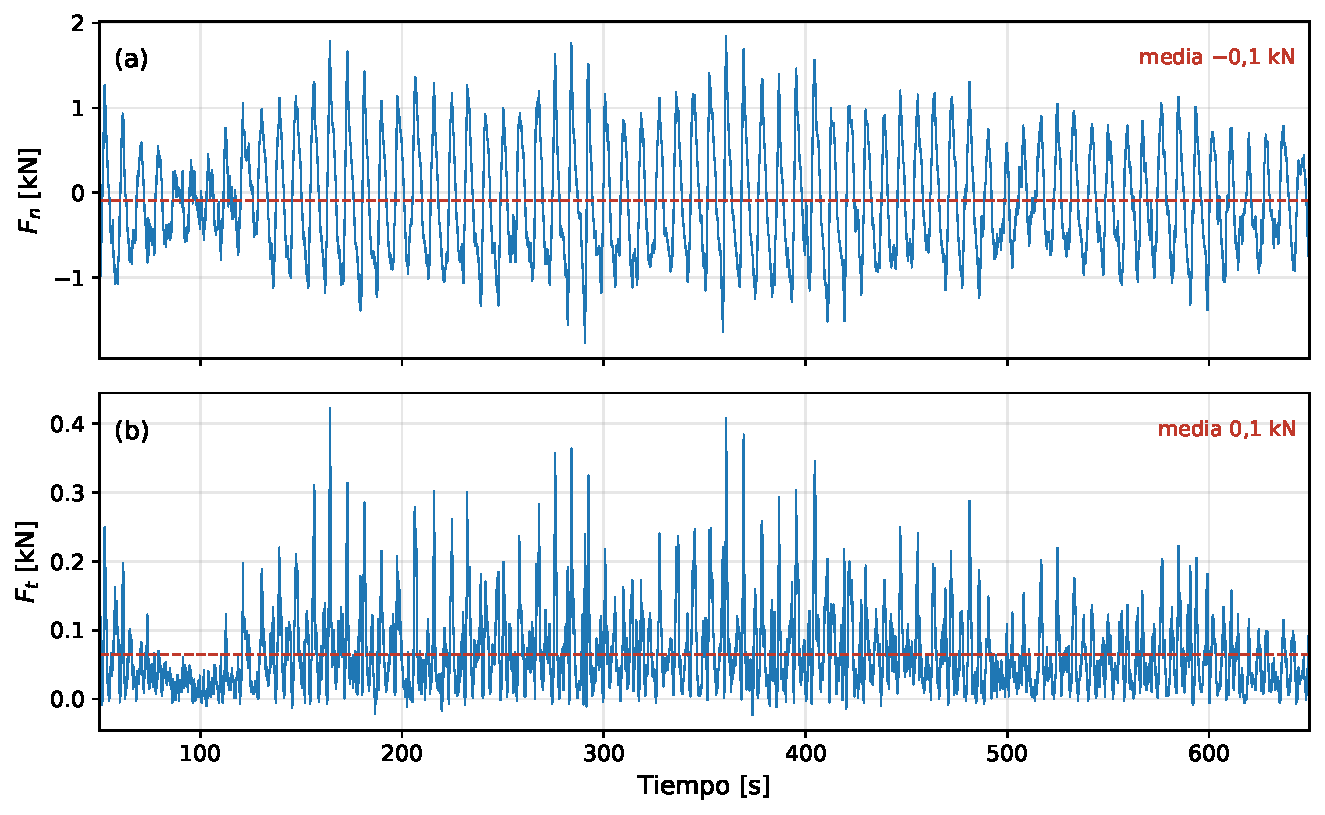
\includegraphics[width=0.85\textwidth]{Figuras/Figuras Anexo Fuerzas/fuerzas_xy_V2_S1.pdf}
    \caption{Fuerzas resultantes (a) $F_x$ y (b) $F_y$ en función del tiempo, $V = 2$~m/s, semilla $1$.}
    \label{fig:anexo_fuerzas_xy_V2_S1}
\end{figure}

\begin{figure}[H]
    \centering
    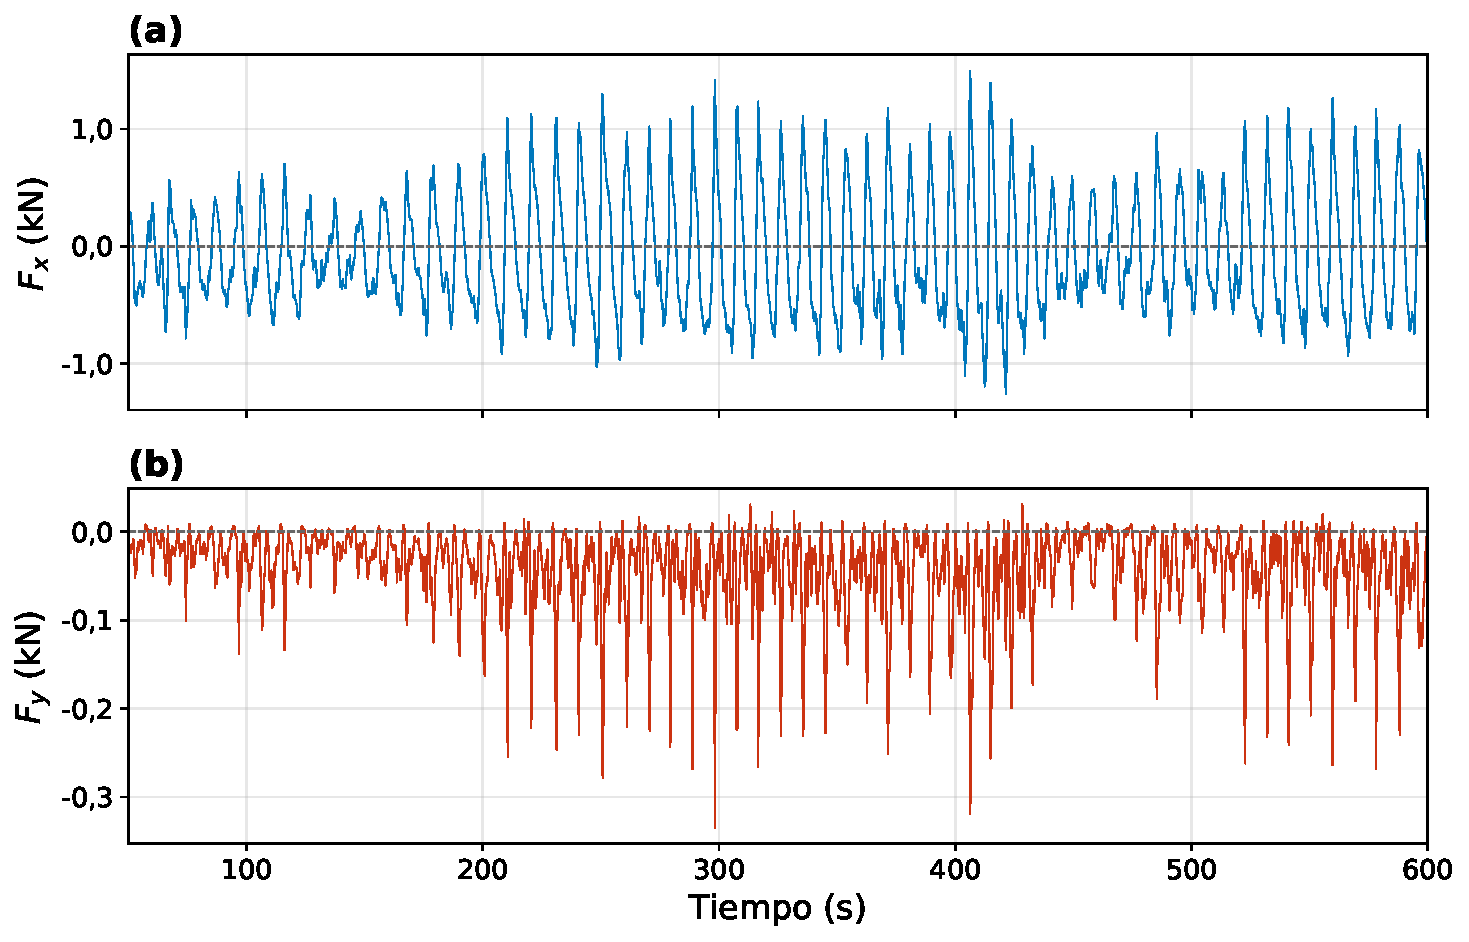
\includegraphics[width=0.85\textwidth]{Figuras/Figuras Anexo Fuerzas/fuerzas_xy_V2_S2.pdf}
    \caption{Fuerzas resultantes (a) $F_x$ y (b) $F_y$ en función del tiempo, $V = 2$~m/s, semilla $2$.}
    \label{fig:anexo_fuerzas_xy_V2_S2}
\end{figure}

\begin{figure}[H]
    \centering
    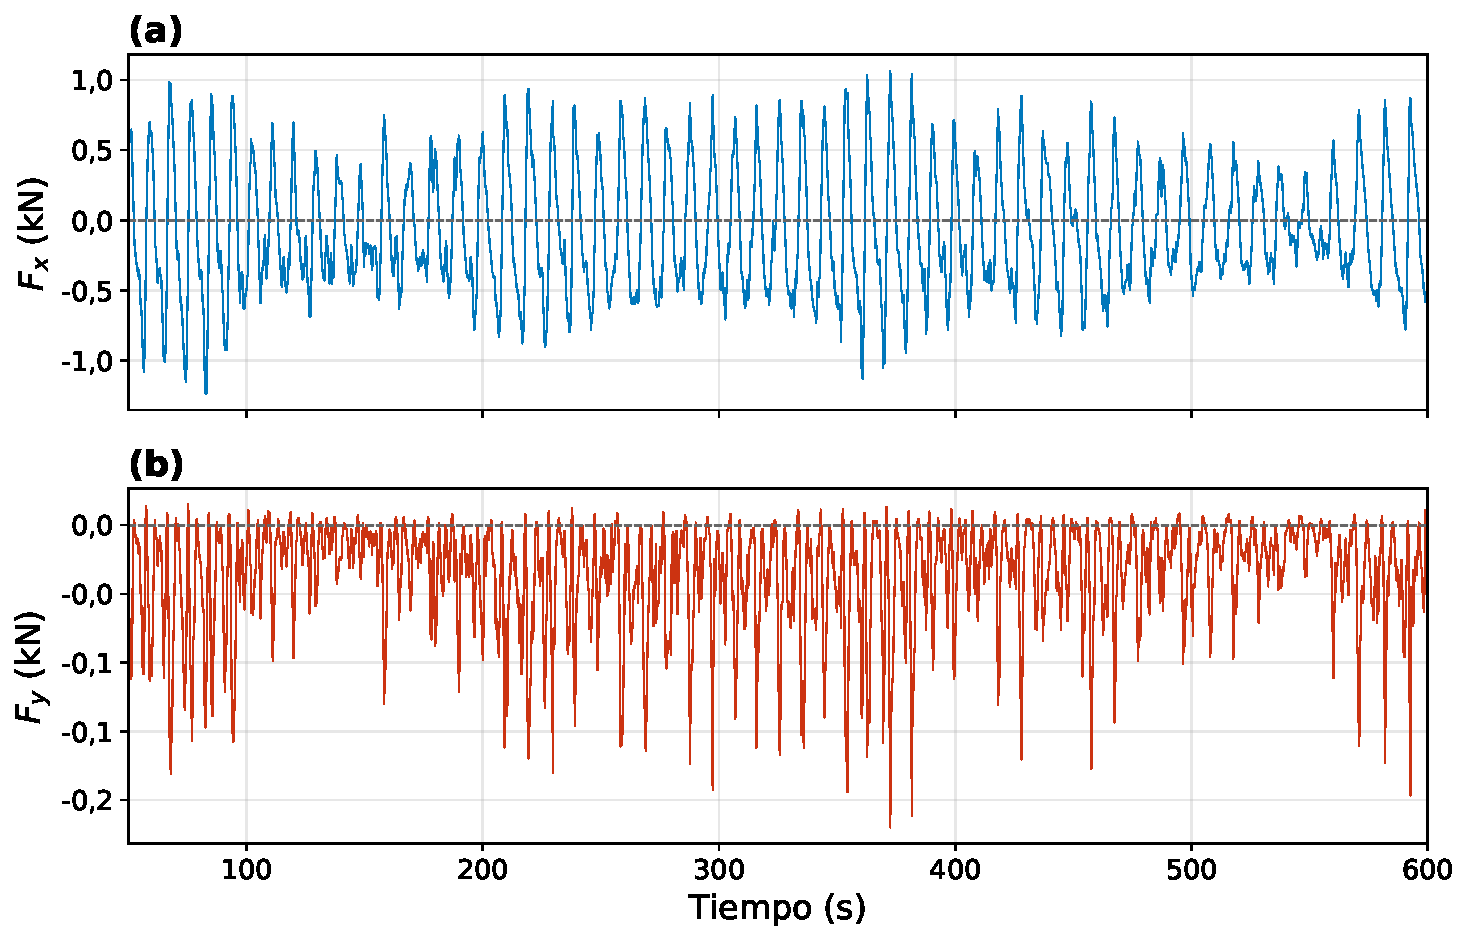
\includegraphics[width=0.85\textwidth]{Figuras/Figuras Anexo Fuerzas/fuerzas_xy_V2_S3.pdf}
    \caption{Fuerzas resultantes (a) $F_x$ y (b) $F_y$ en función del tiempo, $V = 2$~m/s, semilla $3$.}
    \label{fig:anexo_fuerzas_xy_V2_S3}
\end{figure}

\begin{figure}[H]
    \centering
    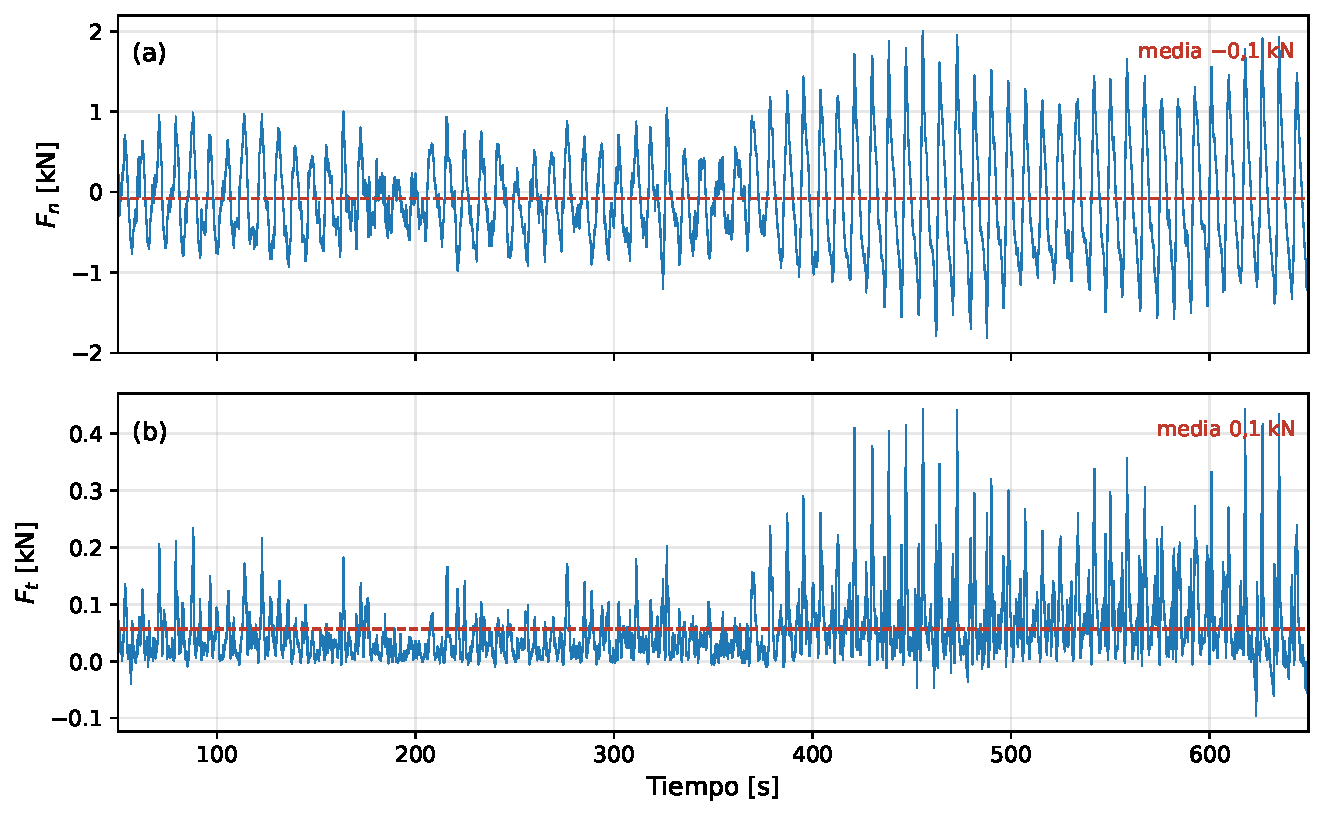
\includegraphics[width=0.85\textwidth]{Figuras/Figuras Anexo Fuerzas/fuerzas_xy_V2_S4.pdf}
    \caption{Fuerzas resultantes (a) $F_x$ y (b) $F_y$ en función del tiempo, $V = 2$~m/s, semilla $4$.}
    \label{fig:anexo_fuerzas_xy_V2_S4}
\end{figure}

\begin{figure}[H]
    \centering
    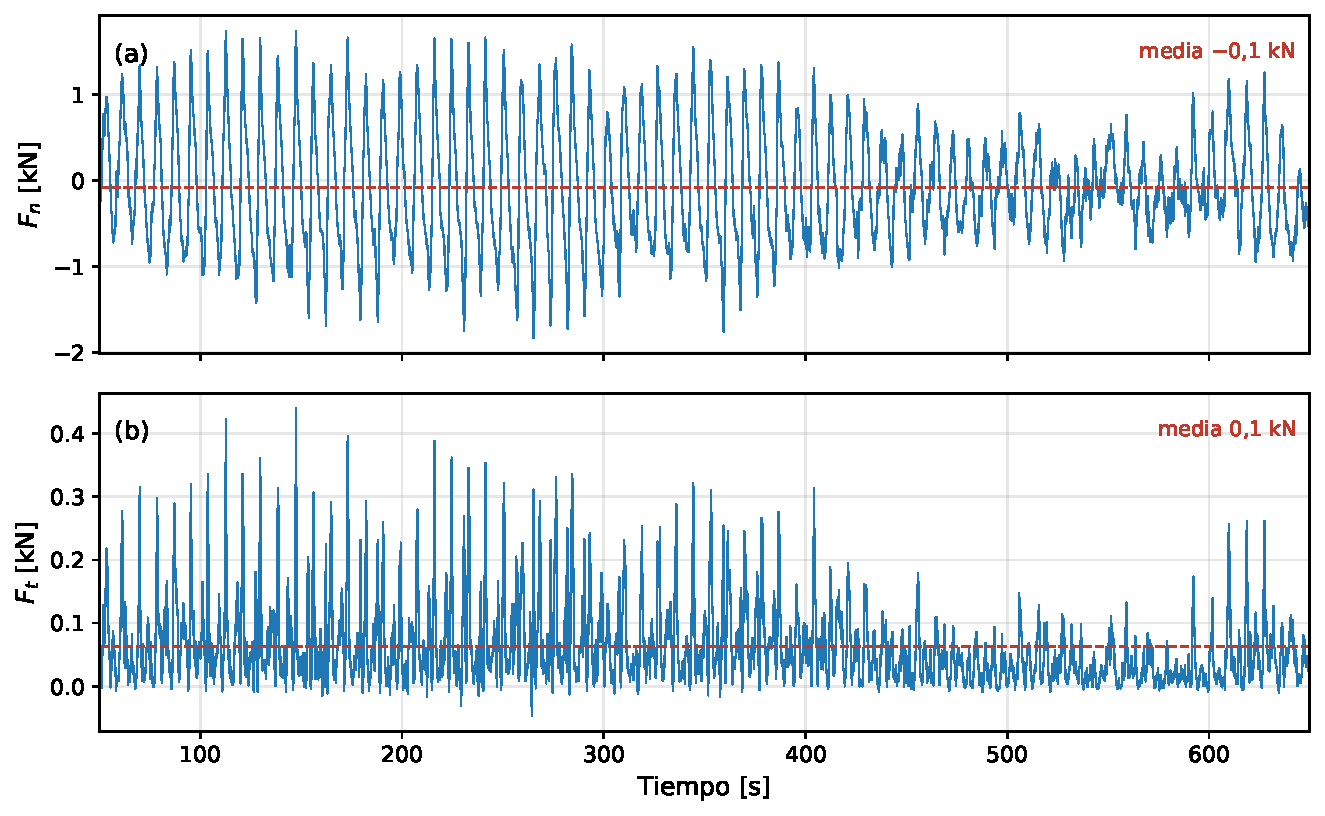
\includegraphics[width=0.85\textwidth]{Figuras/Figuras Anexo Fuerzas/fuerzas_xy_V2_S5.pdf}
    \caption{Fuerzas resultantes (a) $F_x$ y (b) $F_y$ en función del tiempo, $V = 2$~m/s, semilla $5$.}
    \label{fig:anexo_fuerzas_xy_V2_S5}
\end{figure}

\begin{figure}[H]
    \centering
    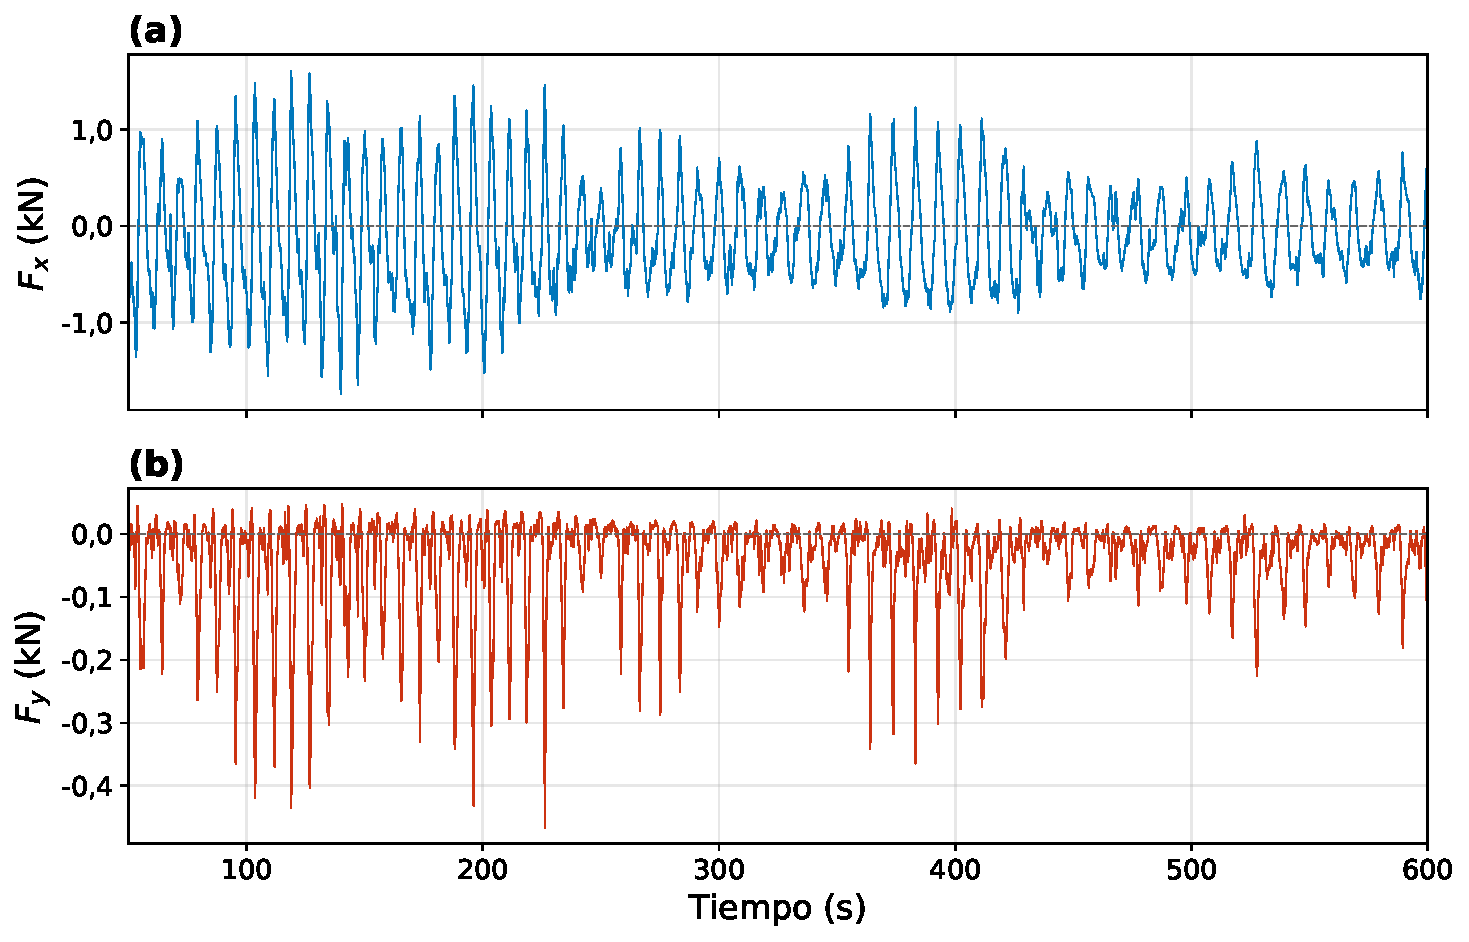
\includegraphics[width=0.85\textwidth]{Figuras/Figuras Anexo Fuerzas/fuerzas_xy_V2_S6.pdf}
    \caption{Fuerzas resultantes (a) $F_x$ y (b) $F_y$ en función del tiempo, $V = 2$~m/s, semilla $6$.}
    \label{fig:anexo_fuerzas_xy_V2_S6}
\end{figure}

\begin{figure}[H]
    \centering
    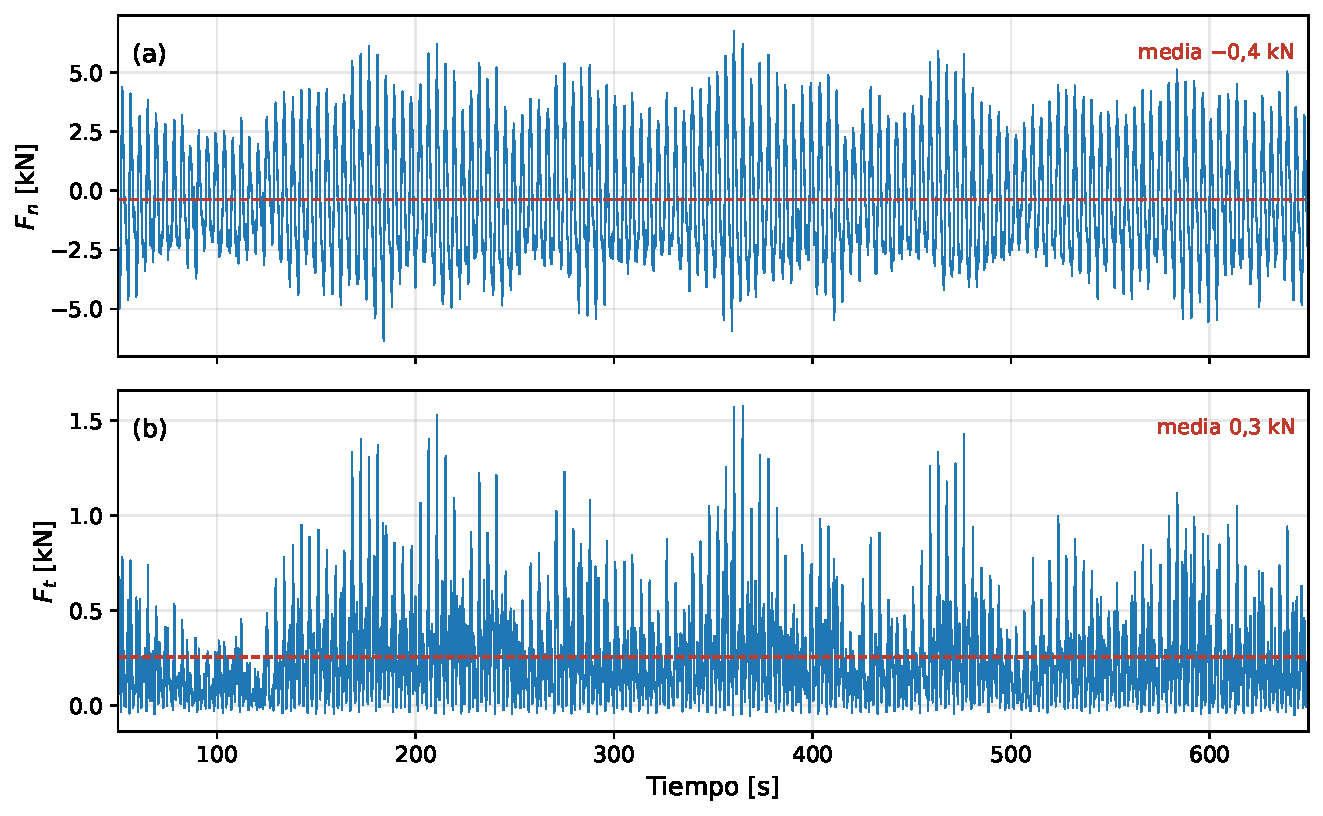
\includegraphics[width=0.85\textwidth]{Figuras/Figuras Anexo Fuerzas/fuerzas_xy_V4_S1.pdf}
    \caption{Fuerzas resultantes (a) $F_x$ y (b) $F_y$ en función del tiempo, $V = 4$~m/s, semilla $1$.}
    \label{fig:anexo_fuerzas_xy_V4_S1}
\end{figure}

\begin{figure}[H]
    \centering
    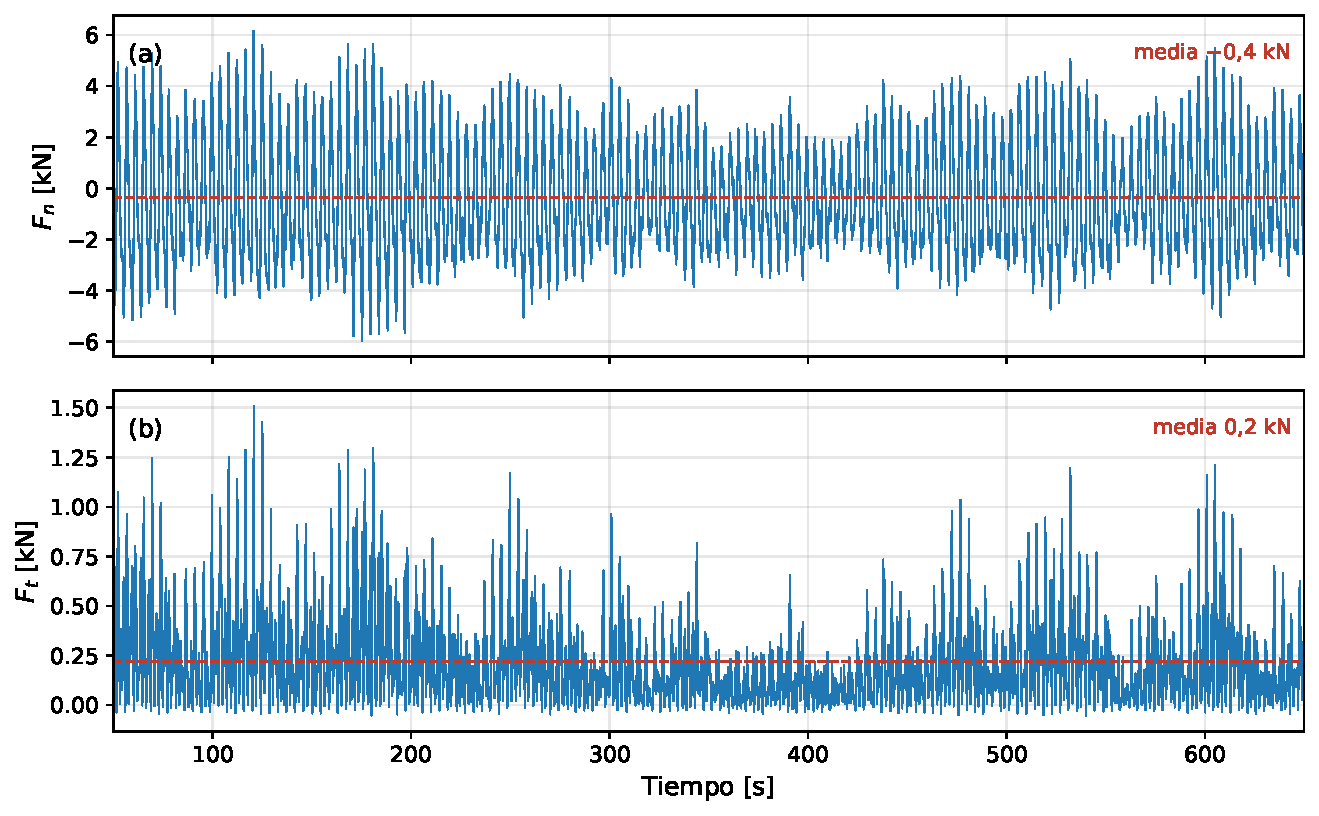
\includegraphics[width=0.85\textwidth]{Figuras/Figuras Anexo Fuerzas/fuerzas_xy_V4_S2.pdf}
    \caption{Fuerzas resultantes (a) $F_x$ y (b) $F_y$ en función del tiempo, $V = 4$~m/s, semilla $2$.}
    \label{fig:anexo_fuerzas_xy_V4_S2}
\end{figure}

\begin{figure}[H]
    \centering
    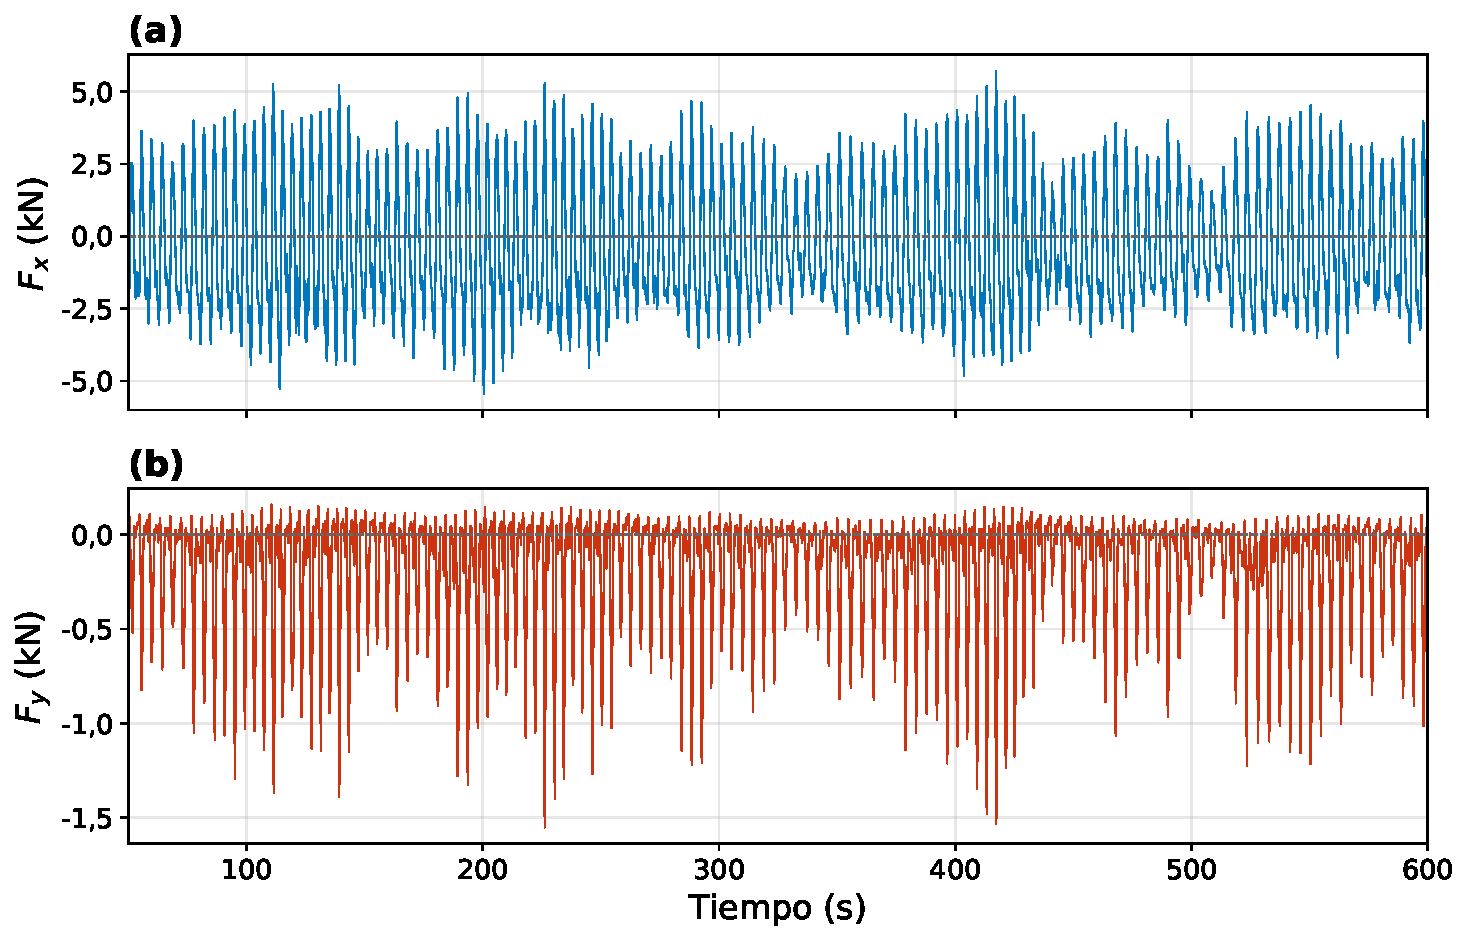
\includegraphics[width=0.85\textwidth]{Figuras/Figuras Anexo Fuerzas/fuerzas_xy_V4_S3.pdf}
    \caption{Fuerzas resultantes (a) $F_x$ y (b) $F_y$ en función del tiempo, $V = 4$~m/s, semilla $3$.}
    \label{fig:anexo_fuerzas_xy_V4_S3}
\end{figure}

\begin{figure}[H]
    \centering
    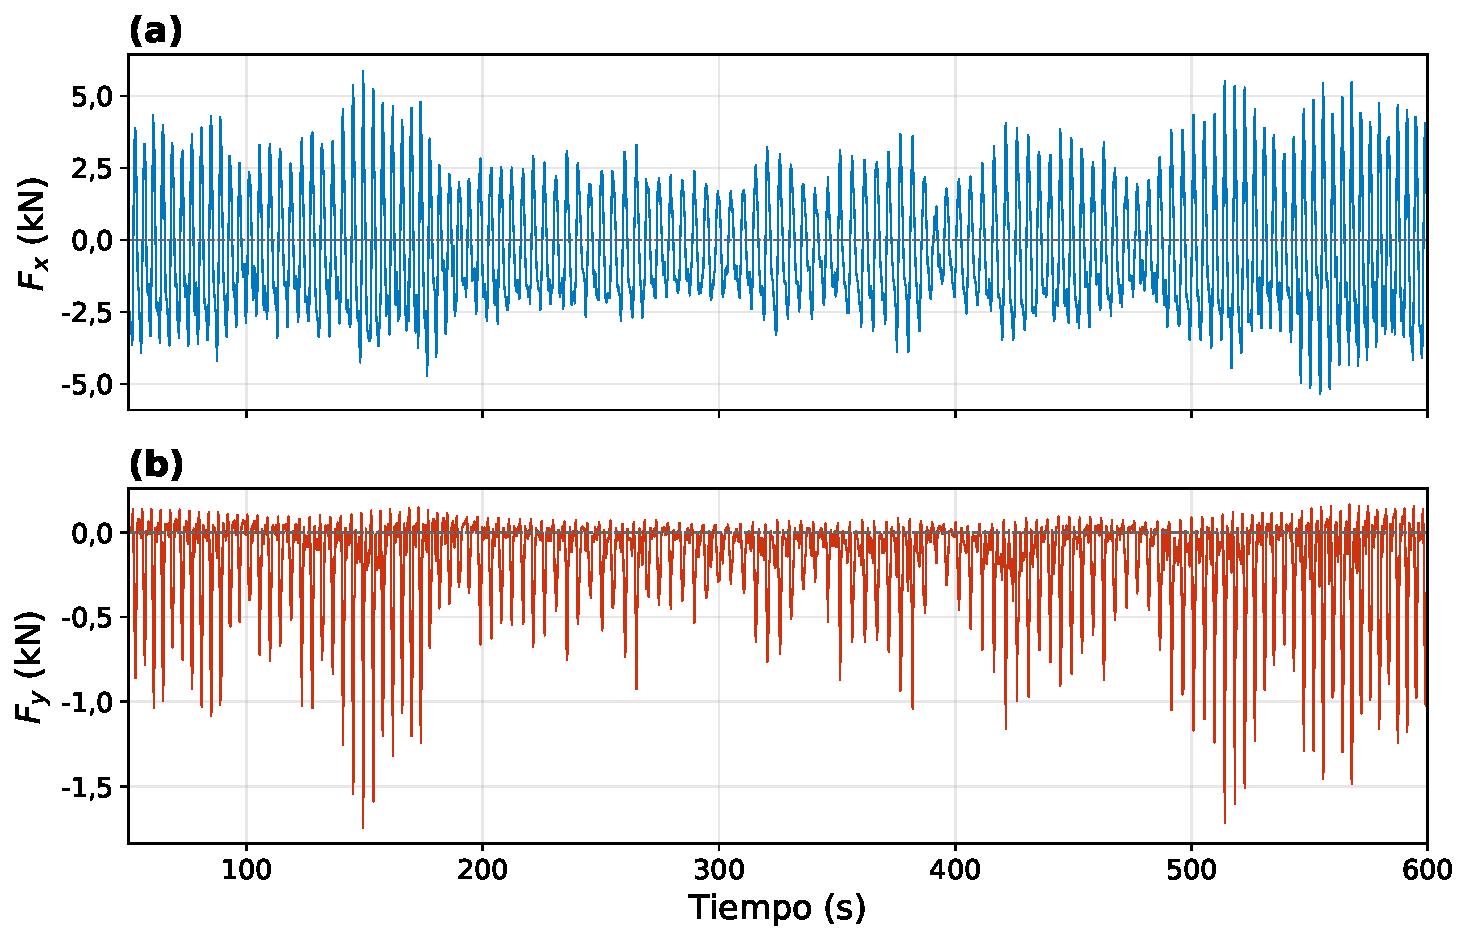
\includegraphics[width=0.85\textwidth]{Figuras/Figuras Anexo Fuerzas/fuerzas_xy_V4_S4.pdf}
    \caption{Fuerzas resultantes (a) $F_x$ y (b) $F_y$ en función del tiempo, $V = 4$~m/s, semilla $4$.}
    \label{fig:anexo_fuerzas_xy_V4_S4}
\end{figure}

\begin{figure}[H]
    \centering
    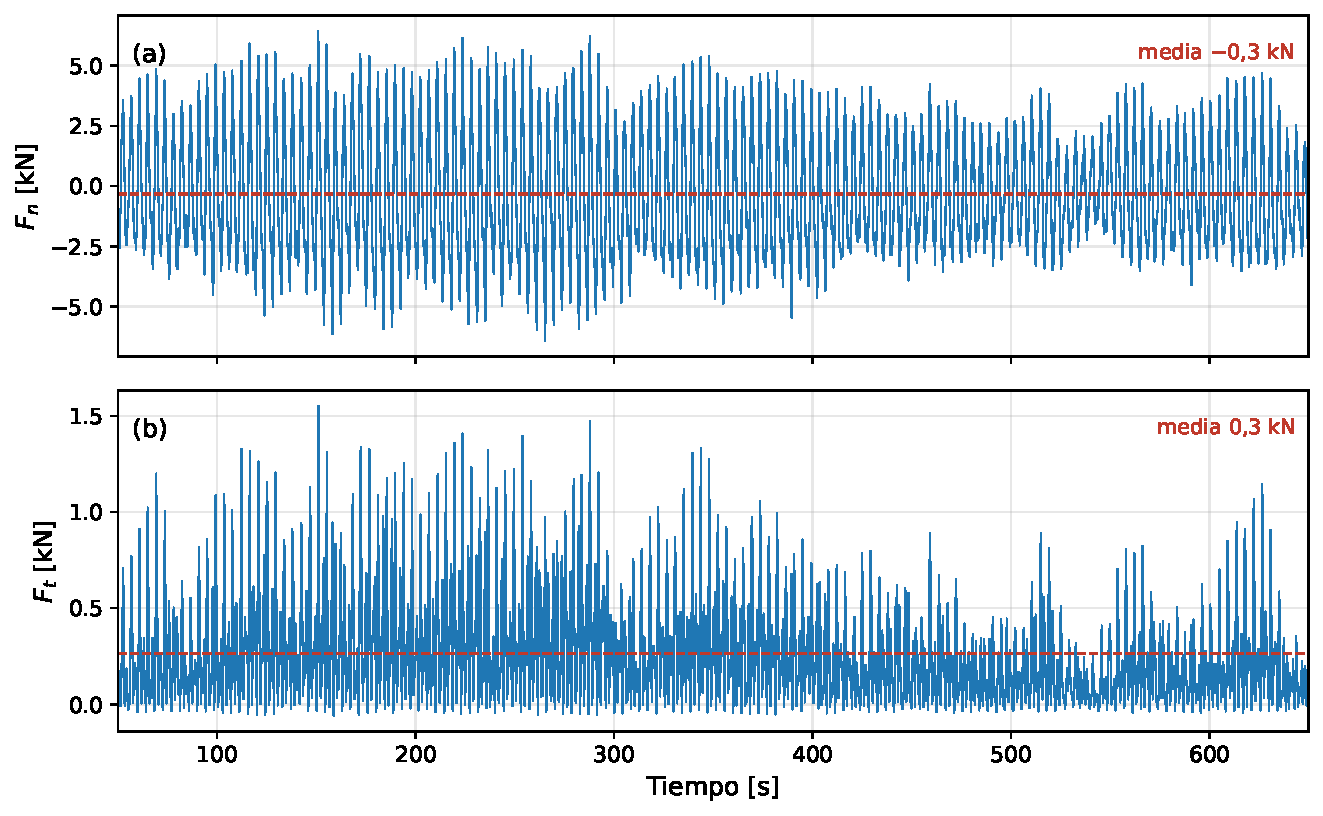
\includegraphics[width=0.85\textwidth]{Figuras/Figuras Anexo Fuerzas/fuerzas_xy_V4_S5.pdf}
    \caption{Fuerzas resultantes (a) $F_x$ y (b) $F_y$ en función del tiempo, $V = 4$~m/s, semilla $5$.}
    \label{fig:anexo_fuerzas_xy_V4_S5}
\end{figure}

\begin{figure}[H]
    \centering
    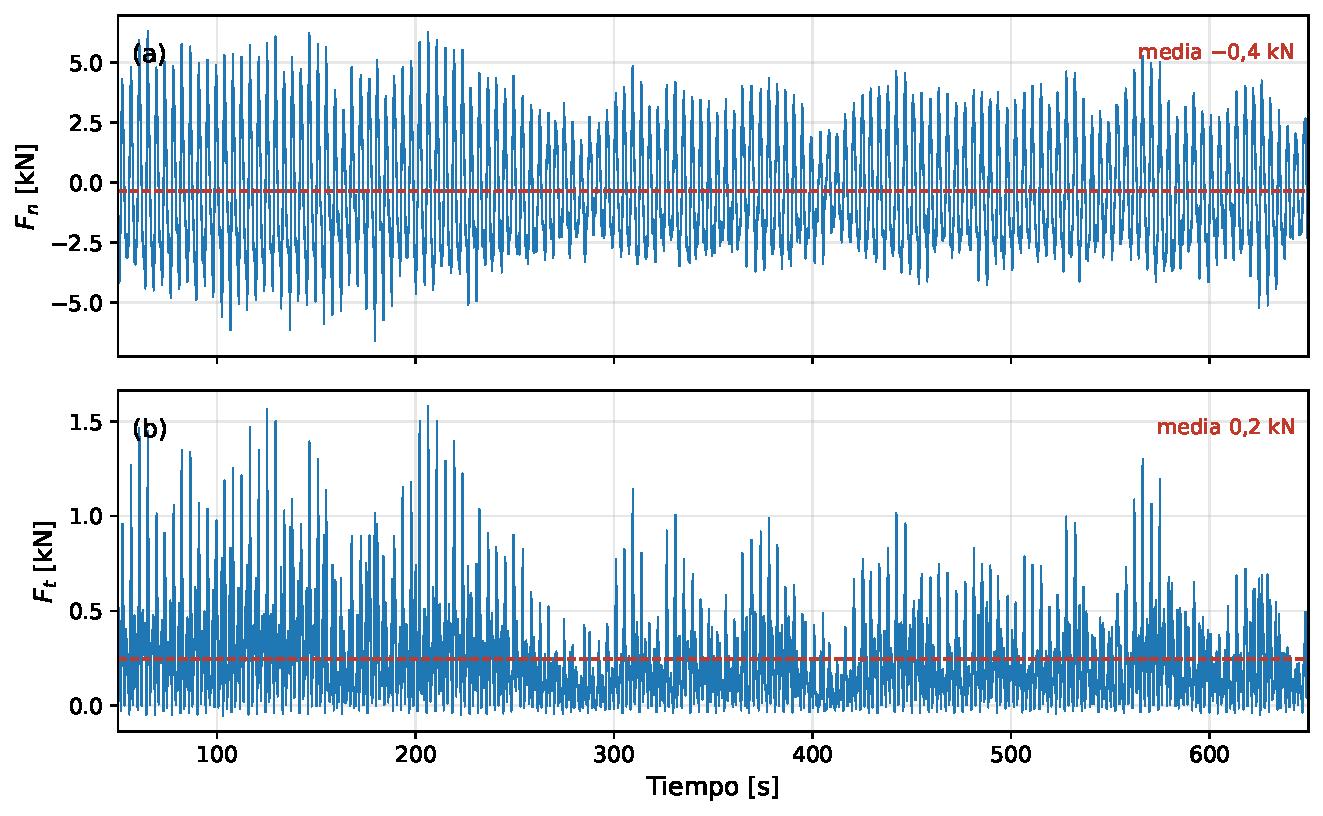
\includegraphics[width=0.85\textwidth]{Figuras/Figuras Anexo Fuerzas/fuerzas_xy_V4_S6.pdf}
    \caption{Fuerzas resultantes (a) $F_x$ y (b) $F_y$ en función del tiempo, $V = 4$~m/s, semilla $6$.}
    \label{fig:anexo_fuerzas_xy_V4_S6}
\end{figure}

\begin{figure}[H]
    \centering
    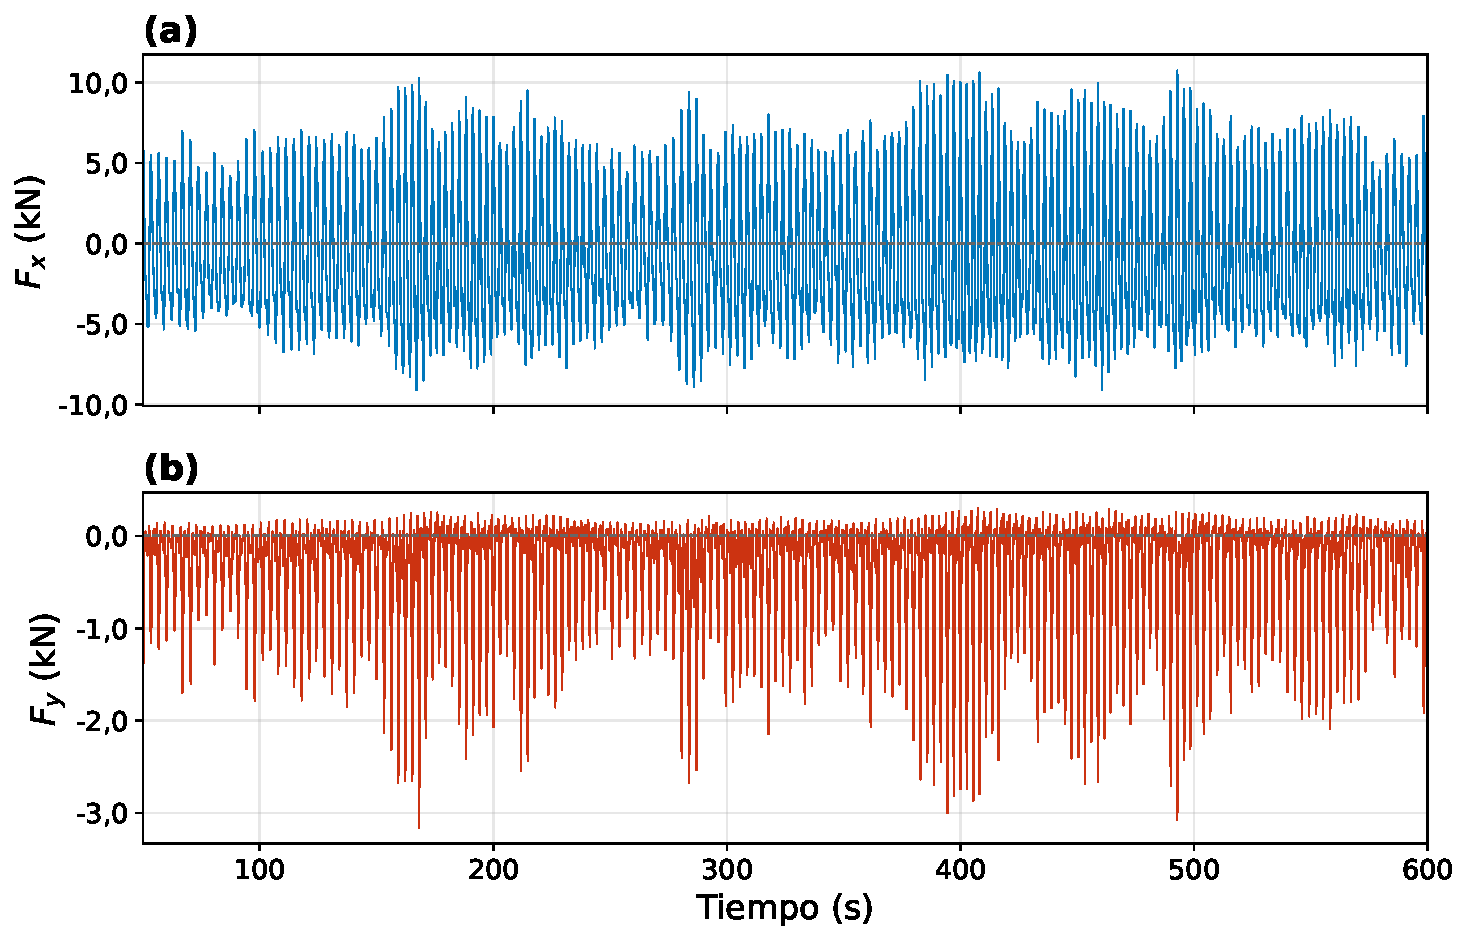
\includegraphics[width=0.85\textwidth]{Figuras/Figuras Anexo Fuerzas/fuerzas_xy_V6_S1.pdf}
    \caption{Fuerzas resultantes (a) $F_x$ y (b) $F_y$ en función del tiempo, $V = 6$~m/s, semilla $1$.}
    \label{fig:anexo_fuerzas_xy_V6_S1}
\end{figure}

\begin{figure}[H]
    \centering
    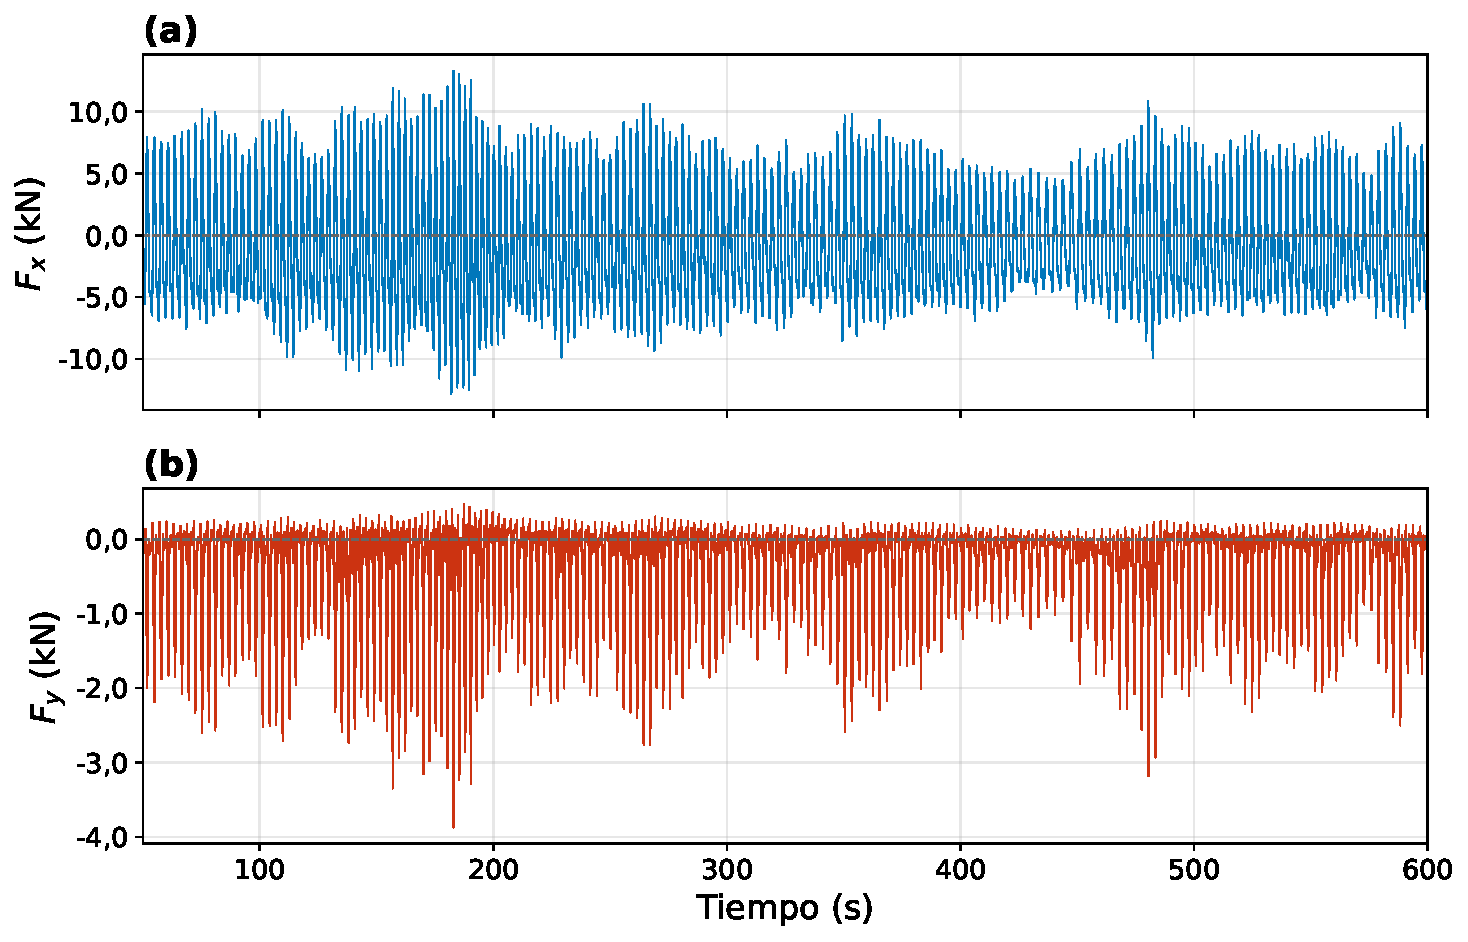
\includegraphics[width=0.85\textwidth]{Figuras/Figuras Anexo Fuerzas/fuerzas_xy_V6_S2.pdf}
    \caption{Fuerzas resultantes (a) $F_x$ y (b) $F_y$ en función del tiempo, $V = 6$~m/s, semilla $2$.}
    \label{fig:anexo_fuerzas_xy_V6_S2}
\end{figure}

\begin{figure}[H]
    \centering
    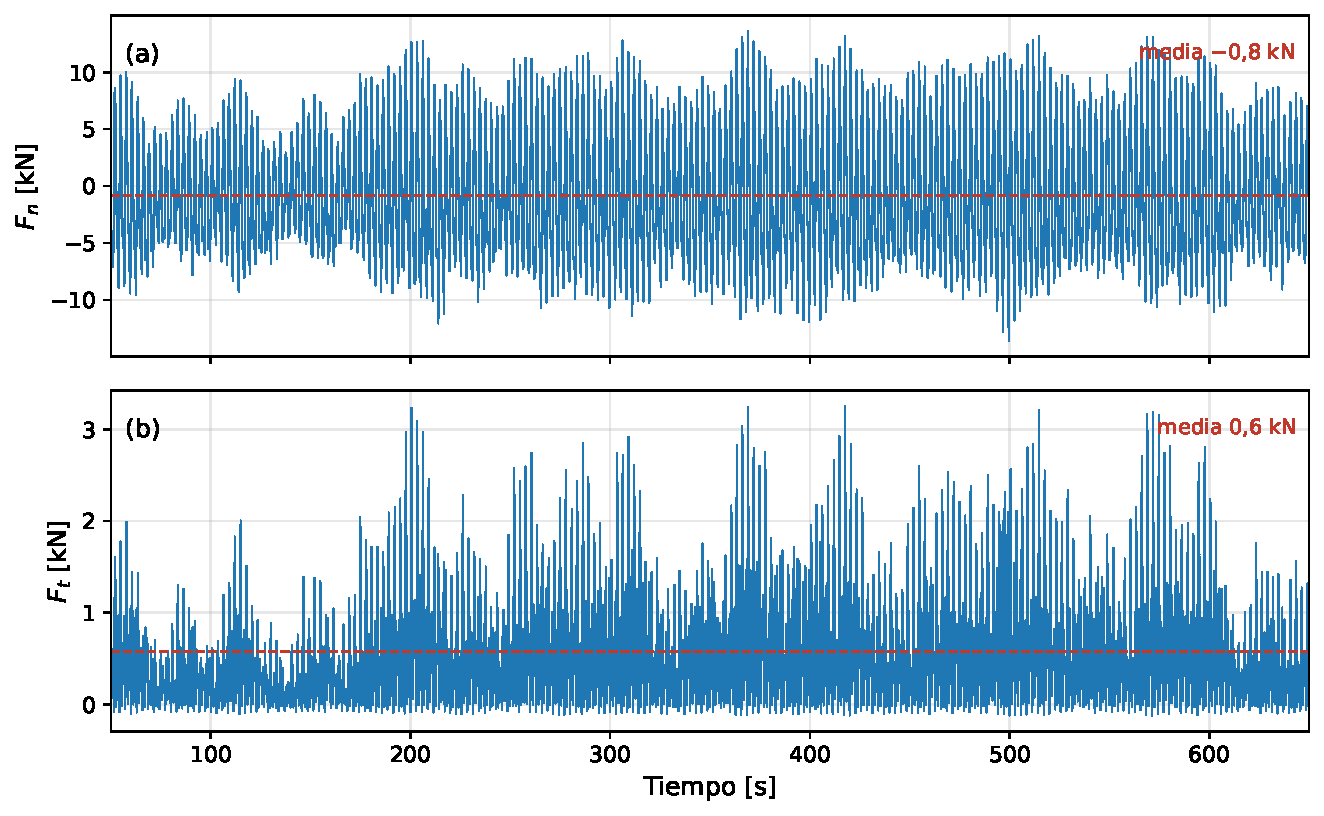
\includegraphics[width=0.85\textwidth]{Figuras/Figuras Anexo Fuerzas/fuerzas_xy_V6_S3.pdf}
    \caption{Fuerzas resultantes (a) $F_x$ y (b) $F_y$ en función del tiempo, $V = 6$~m/s, semilla $3$.}
    \label{fig:anexo_fuerzas_xy_V6_S3}
\end{figure}

\begin{figure}[H]
    \centering
    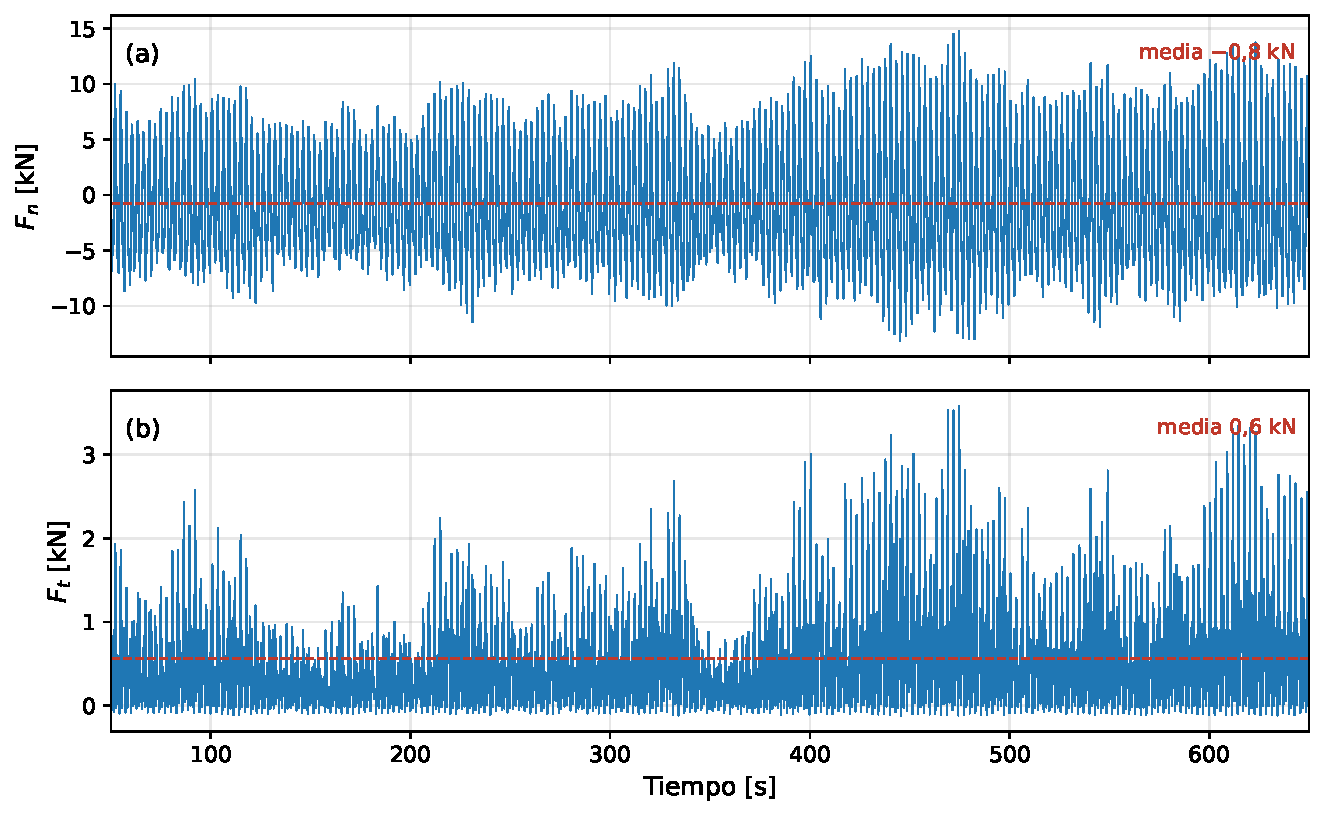
\includegraphics[width=0.85\textwidth]{Figuras/Figuras Anexo Fuerzas/fuerzas_xy_V6_S4.pdf}
    \caption{Fuerzas resultantes (a) $F_x$ y (b) $F_y$ en función del tiempo, $V = 6$~m/s, semilla $4$.}
    \label{fig:anexo_fuerzas_xy_V6_S4}
\end{figure}

\begin{figure}[H]
    \centering
    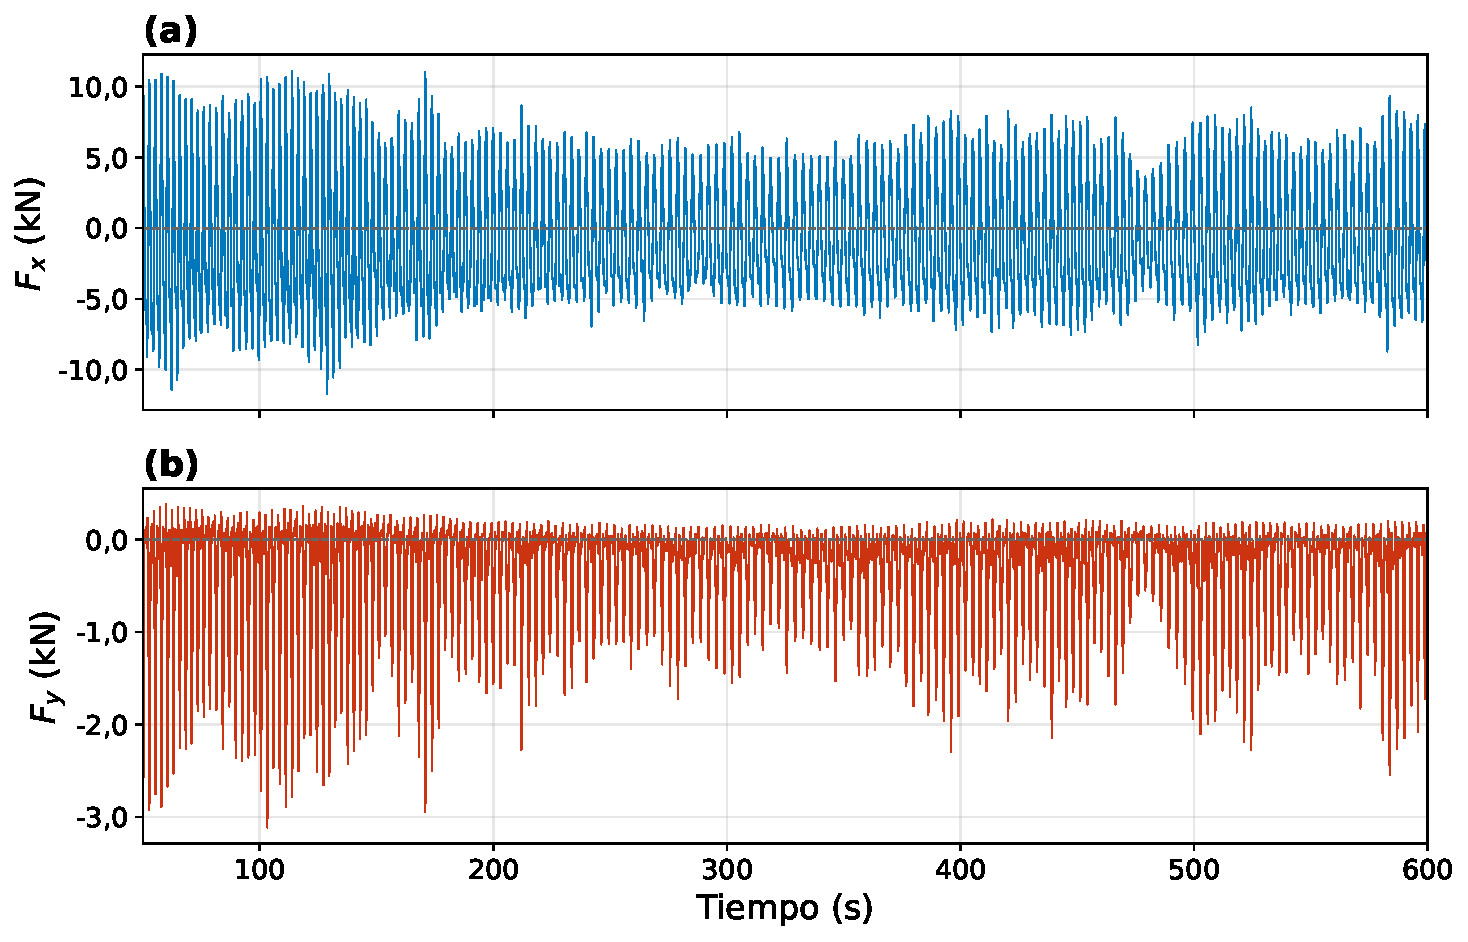
\includegraphics[width=0.85\textwidth]{Figuras/Figuras Anexo Fuerzas/fuerzas_xy_V6_S5.pdf}
    \caption{Fuerzas resultantes (a) $F_x$ y (b) $F_y$ en función del tiempo, $V = 6$~m/s, semilla $5$.}
    \label{fig:anexo_fuerzas_xy_V6_S5}
\end{figure}

\begin{figure}[H]
    \centering
    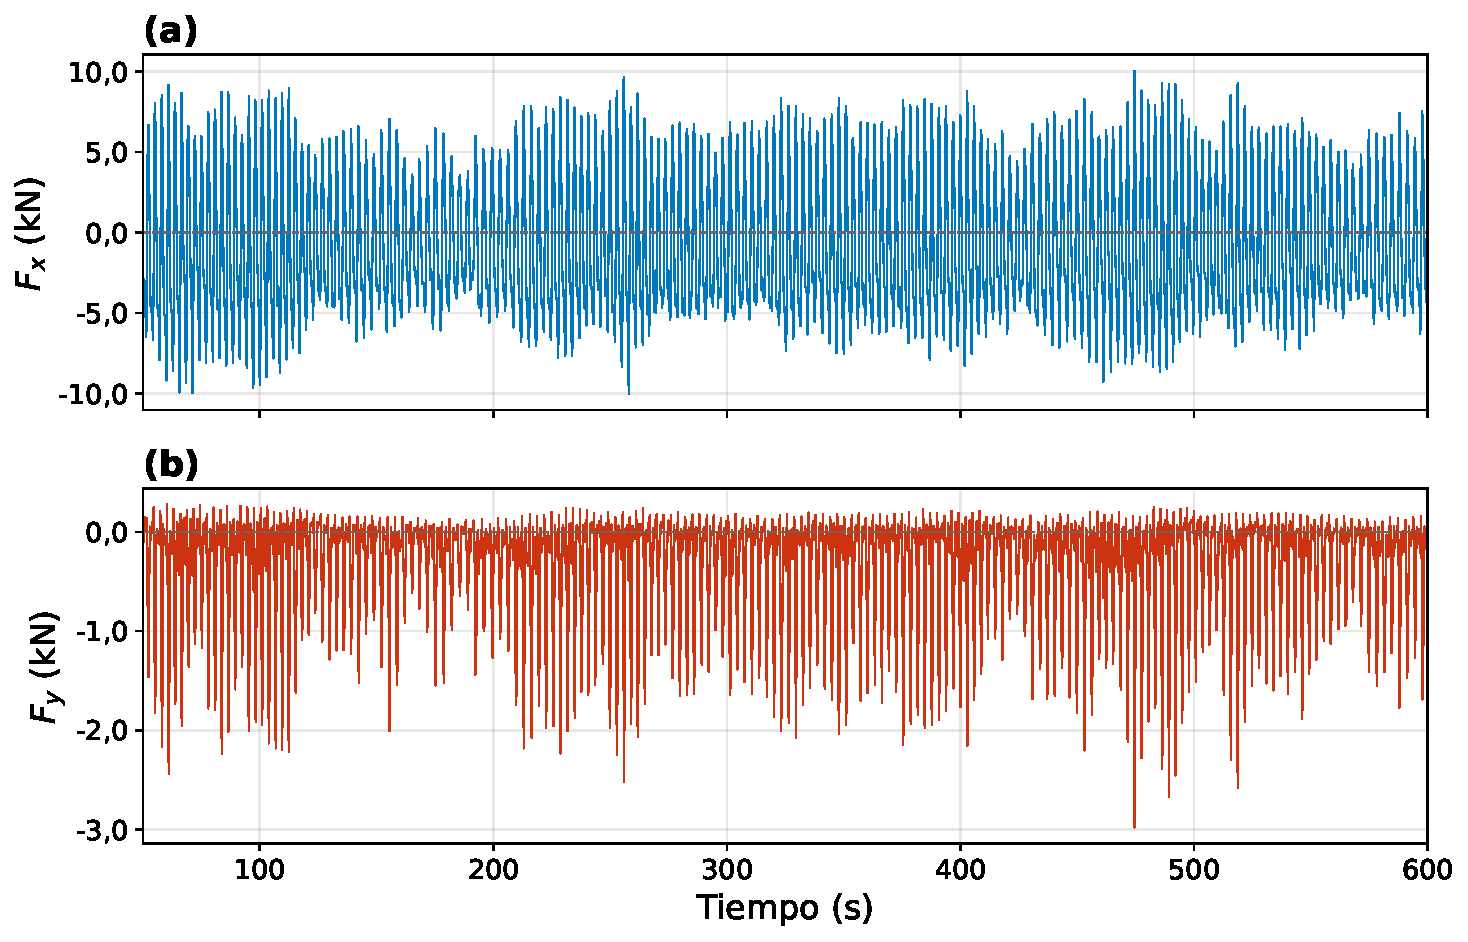
\includegraphics[width=0.85\textwidth]{Figuras/Figuras Anexo Fuerzas/fuerzas_xy_V6_S6.pdf}
    \caption{Fuerzas resultantes (a) $F_x$ y (b) $F_y$ en función del tiempo, $V = 6$~m/s, semilla $6$.}
    \label{fig:anexo_fuerzas_xy_V6_S6}
\end{figure}

\begin{figure}[H]
    \centering
    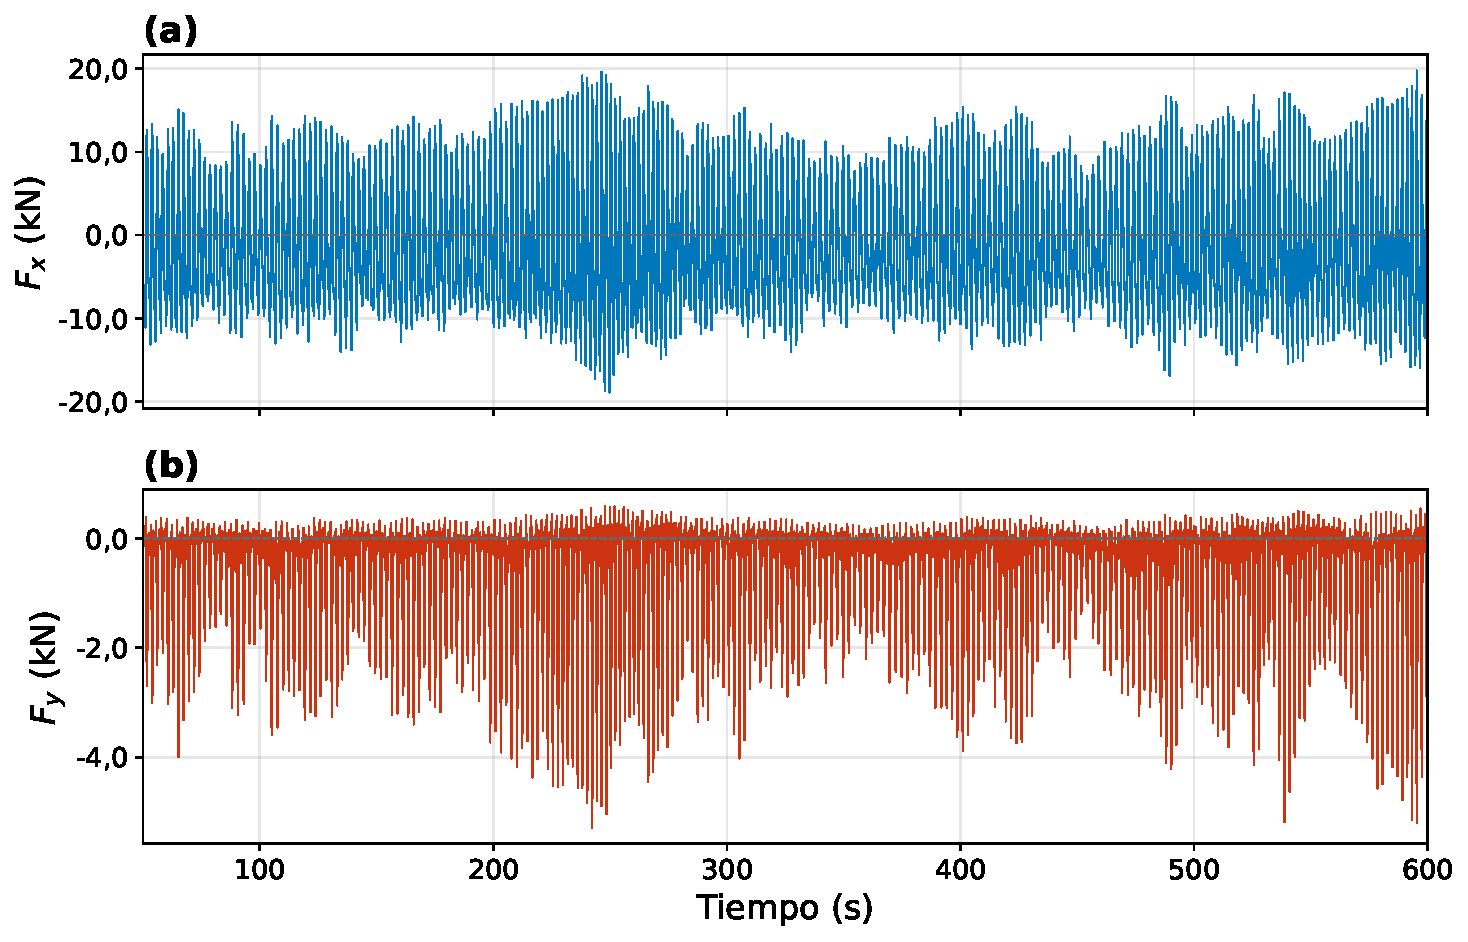
\includegraphics[width=0.85\textwidth]{Figuras/Figuras Anexo Fuerzas/fuerzas_xy_V8_S1.pdf}
    \caption{Fuerzas resultantes (a) $F_x$ y (b) $F_y$ en función del tiempo, $V = 8$~m/s, semilla $1$.}
    \label{fig:anexo_fuerzas_xy_V8_S1}
\end{figure}

\begin{figure}[H]
    \centering
    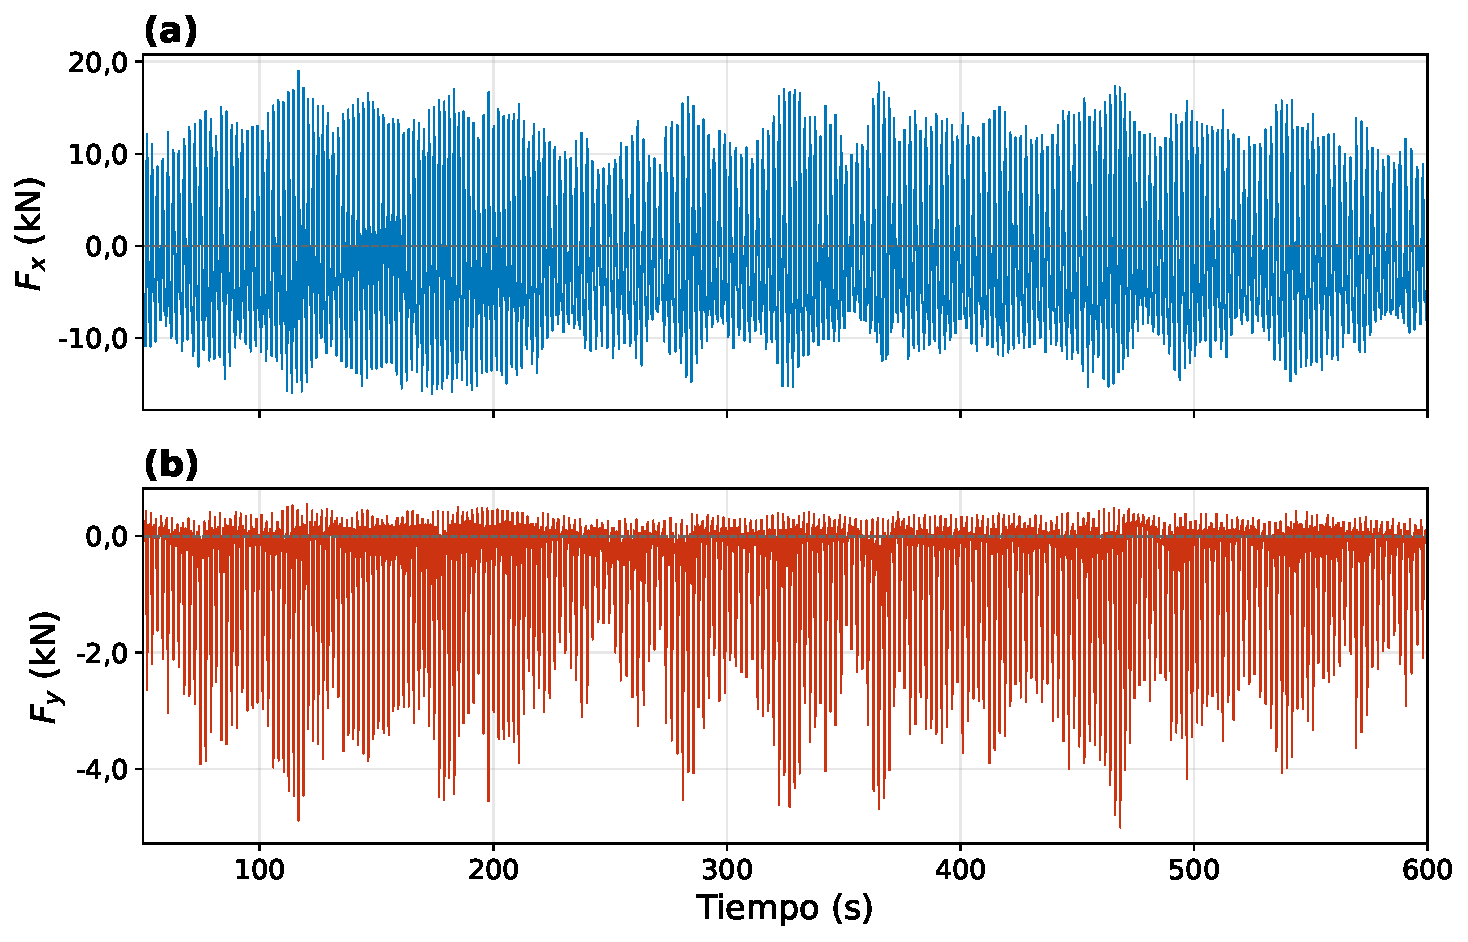
\includegraphics[width=0.85\textwidth]{Figuras/Figuras Anexo Fuerzas/fuerzas_xy_V8_S2.pdf}
    \caption{Fuerzas resultantes (a) $F_x$ y (b) $F_y$ en función del tiempo, $V = 8$~m/s, semilla $2$.}
    \label{fig:anexo_fuerzas_xy_V8_S2}
\end{figure}

\begin{figure}[H]
    \centering
    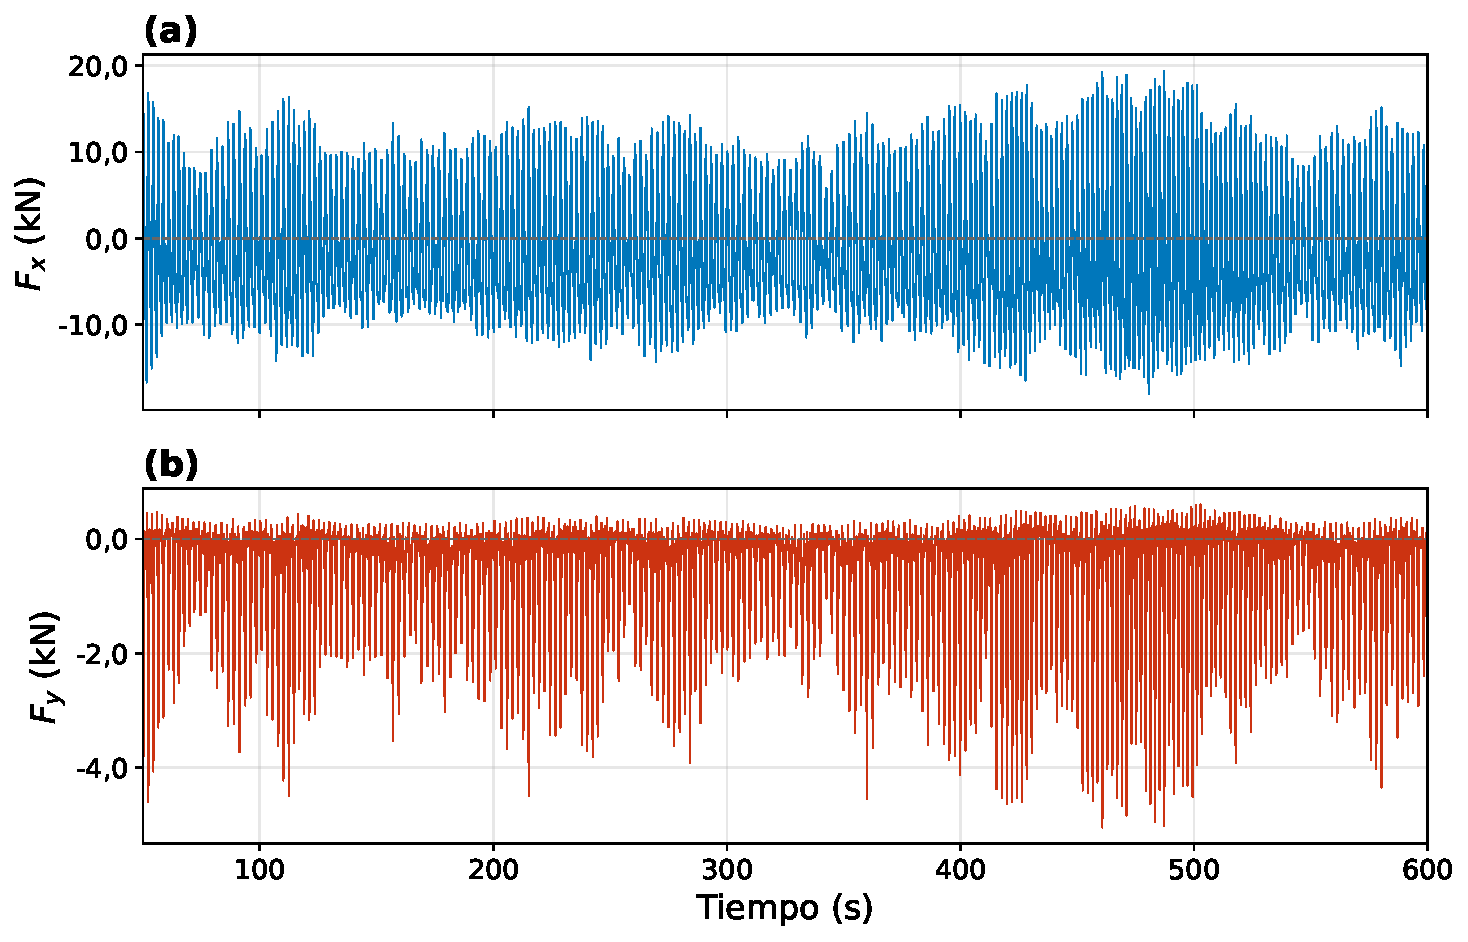
\includegraphics[width=0.85\textwidth]{Figuras/Figuras Anexo Fuerzas/fuerzas_xy_V8_S3.pdf}
    \caption{Fuerzas resultantes (a) $F_x$ y (b) $F_y$ en función del tiempo, $V = 8$~m/s, semilla $3$.}
    \label{fig:anexo_fuerzas_xy_V8_S3}
\end{figure}

\begin{figure}[H]
    \centering
    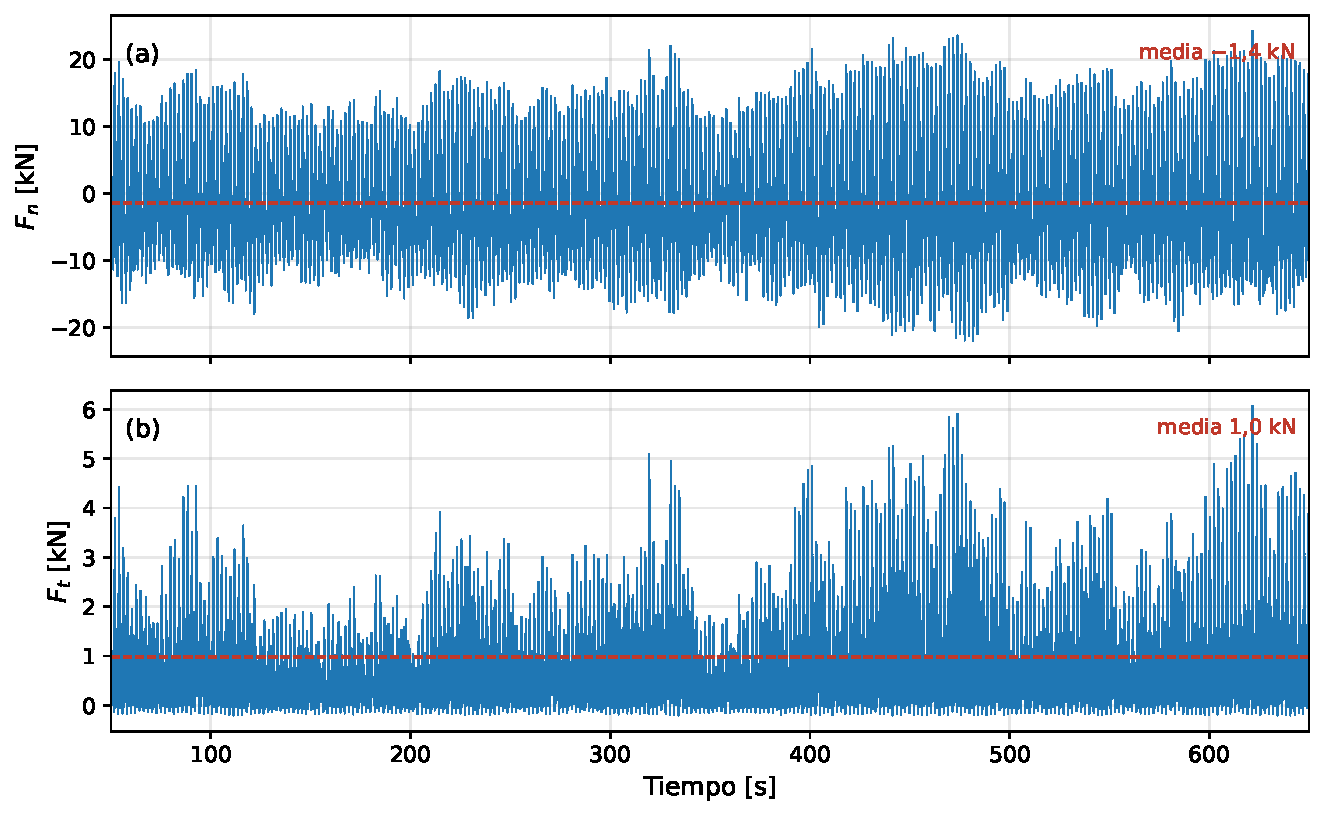
\includegraphics[width=0.85\textwidth]{Figuras/Figuras Anexo Fuerzas/fuerzas_xy_V8_S4.pdf}
    \caption{Fuerzas resultantes (a) $F_x$ y (b) $F_y$ en función del tiempo, $V = 8$~m/s, semilla $4$.}
    \label{fig:anexo_fuerzas_xy_V8_S4}
\end{figure}

\begin{figure}[H]
    \centering
    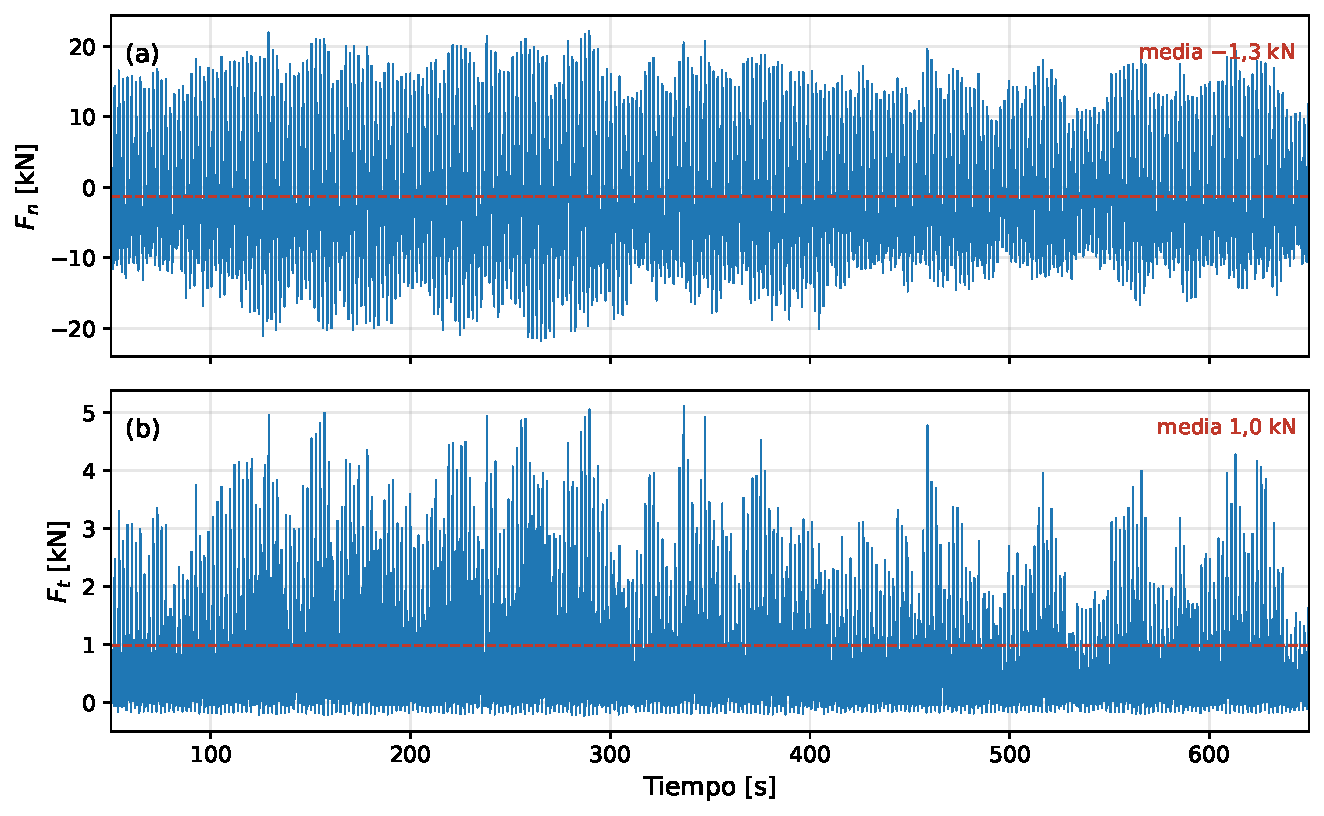
\includegraphics[width=0.85\textwidth]{Figuras/Figuras Anexo Fuerzas/fuerzas_xy_V8_S5.pdf}
    \caption{Fuerzas resultantes (a) $F_x$ y (b) $F_y$ en función del tiempo, $V = 8$~m/s, semilla $5$.}
    \label{fig:anexo_fuerzas_xy_V8_S5}
\end{figure}

\begin{figure}[H]
    \centering
    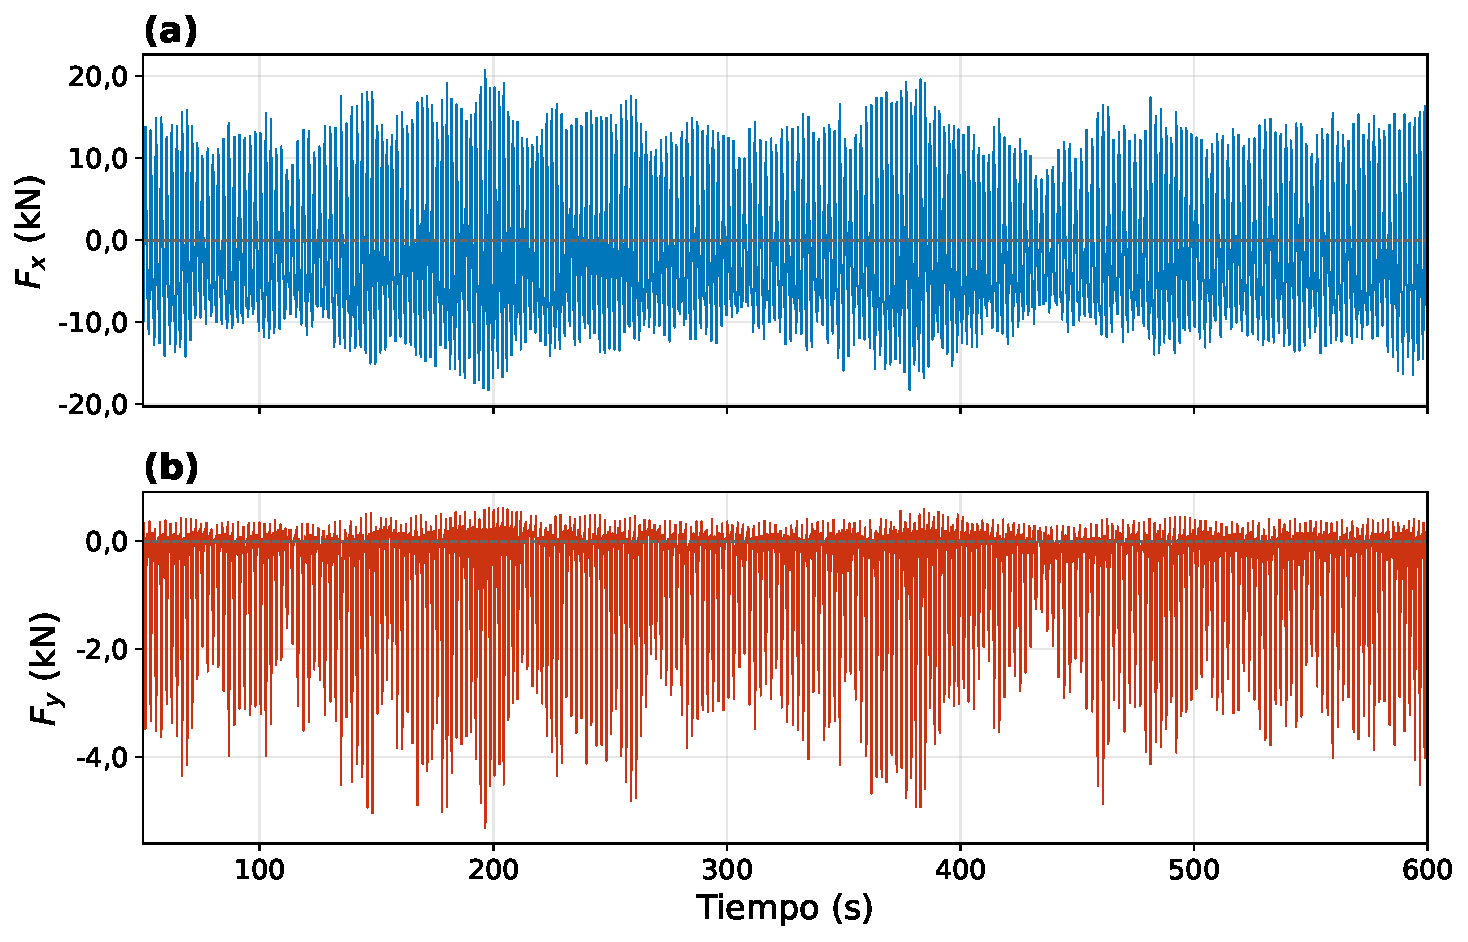
\includegraphics[width=0.85\textwidth]{Figuras/Figuras Anexo Fuerzas/fuerzas_xy_V8_S6.pdf}
    \caption{Fuerzas resultantes (a) $F_x$ y (b) $F_y$ en función del tiempo, $V = 8$~m/s, semilla $6$.}
    \label{fig:anexo_fuerzas_xy_V8_S6}
\end{figure}

\begin{figure}[H]
    \centering
    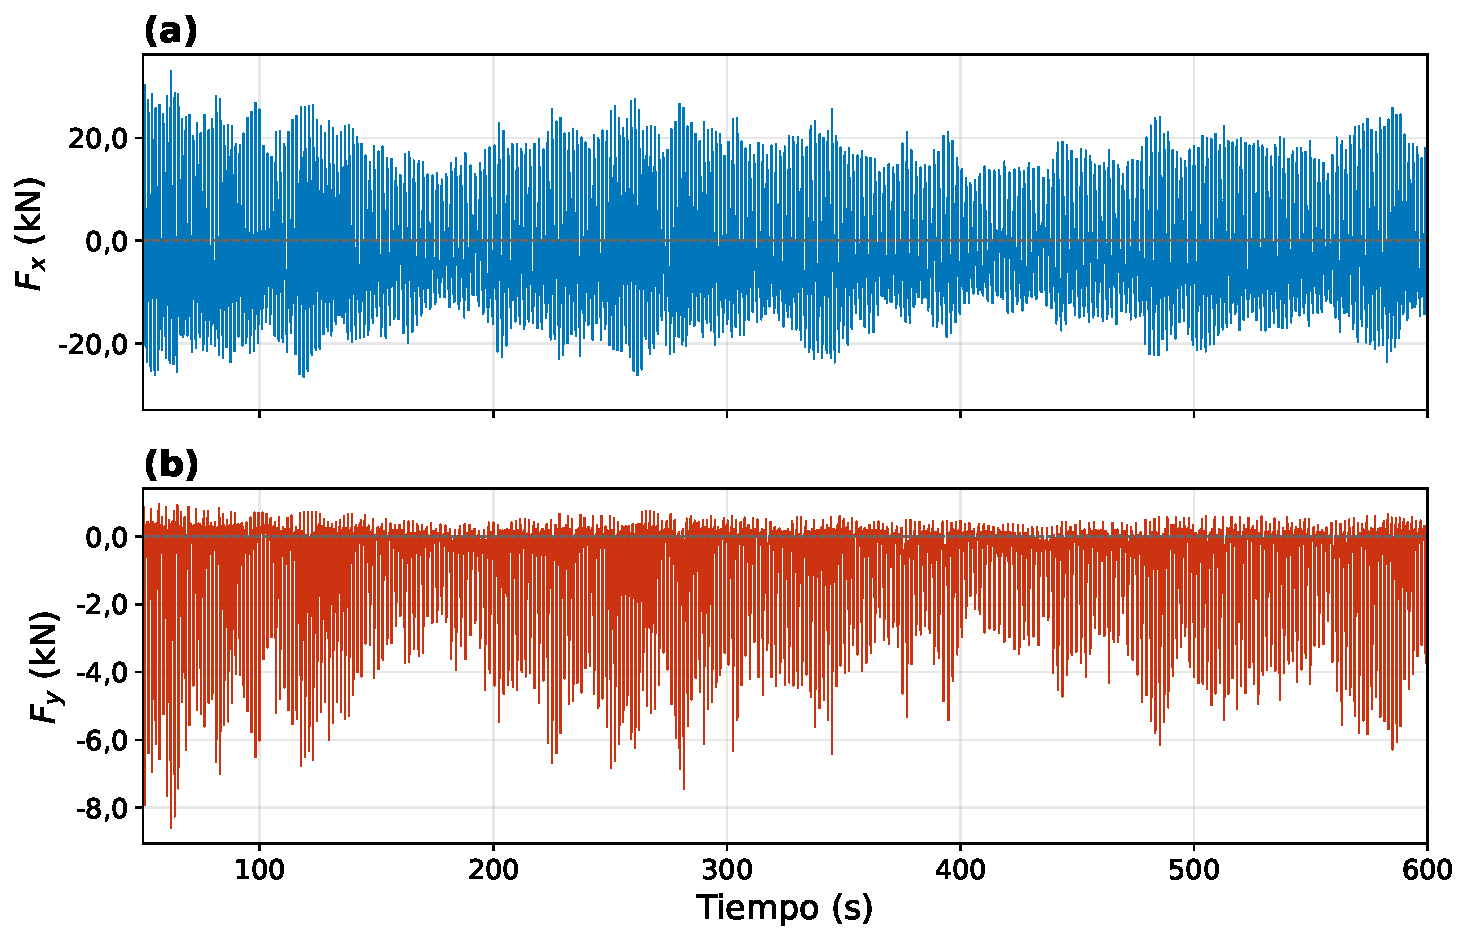
\includegraphics[width=0.85\textwidth]{Figuras/Figuras Anexo Fuerzas/fuerzas_xy_V10_S1.pdf}
    \caption{Fuerzas resultantes (a) $F_x$ y (b) $F_y$ en función del tiempo, $V = 10$~m/s, semilla $1$.}
    \label{fig:anexo_fuerzas_xy_V10_S1}
\end{figure}

\begin{figure}[H]
    \centering
    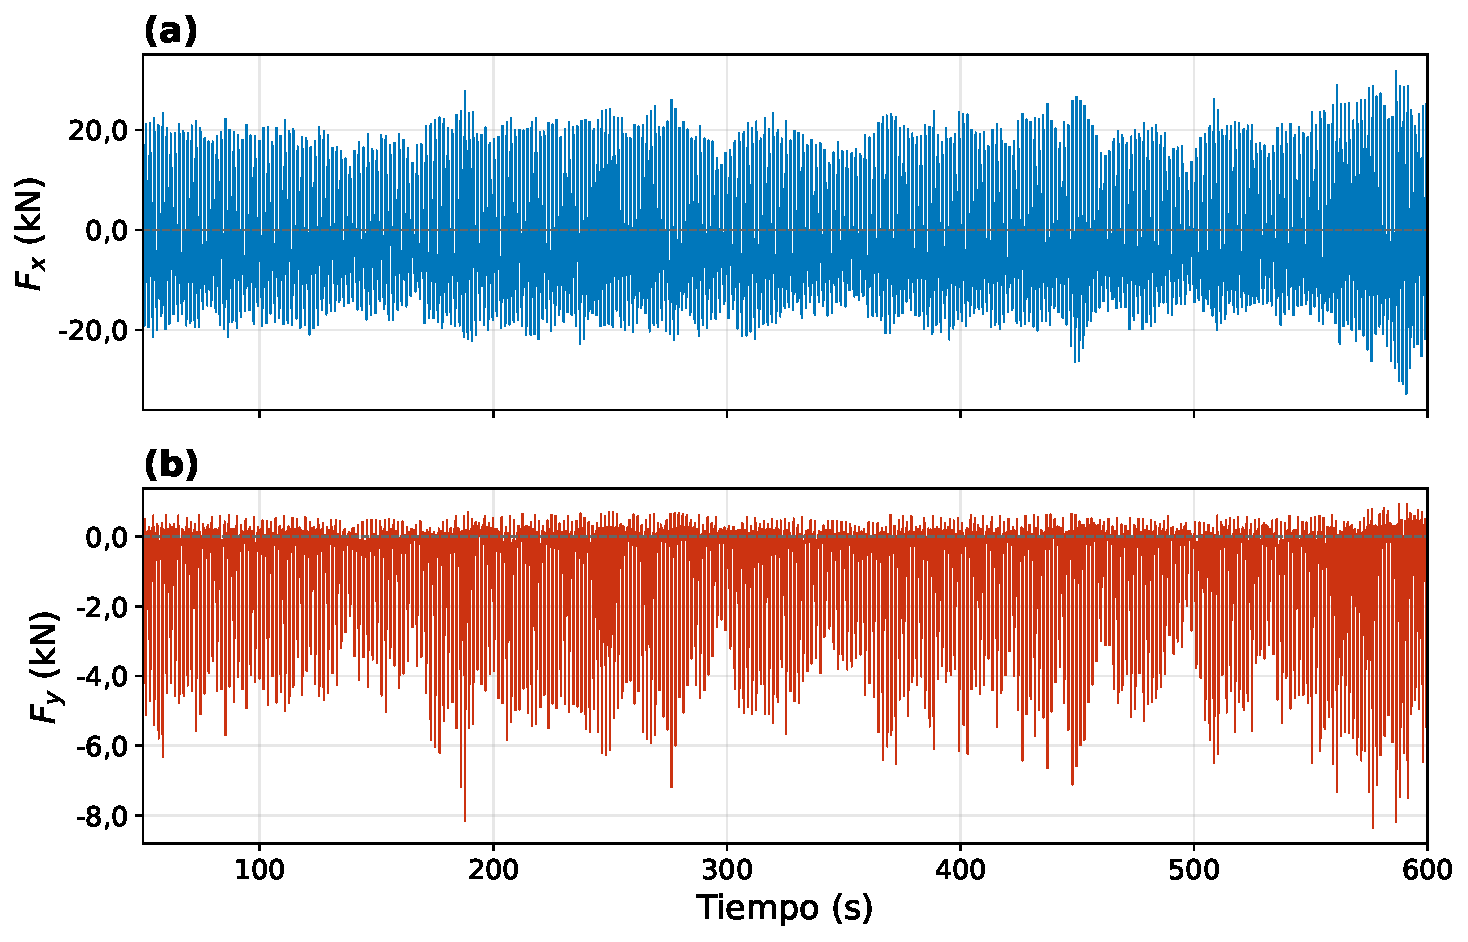
\includegraphics[width=0.85\textwidth]{Figuras/Figuras Anexo Fuerzas/fuerzas_xy_V10_S2.pdf}
    \caption{Fuerzas resultantes (a) $F_x$ y (b) $F_y$ en función del tiempo, $V = 10$~m/s, semilla $2$.}
    \label{fig:anexo_fuerzas_xy_V10_S2}
\end{figure}

\begin{figure}[H]
    \centering
    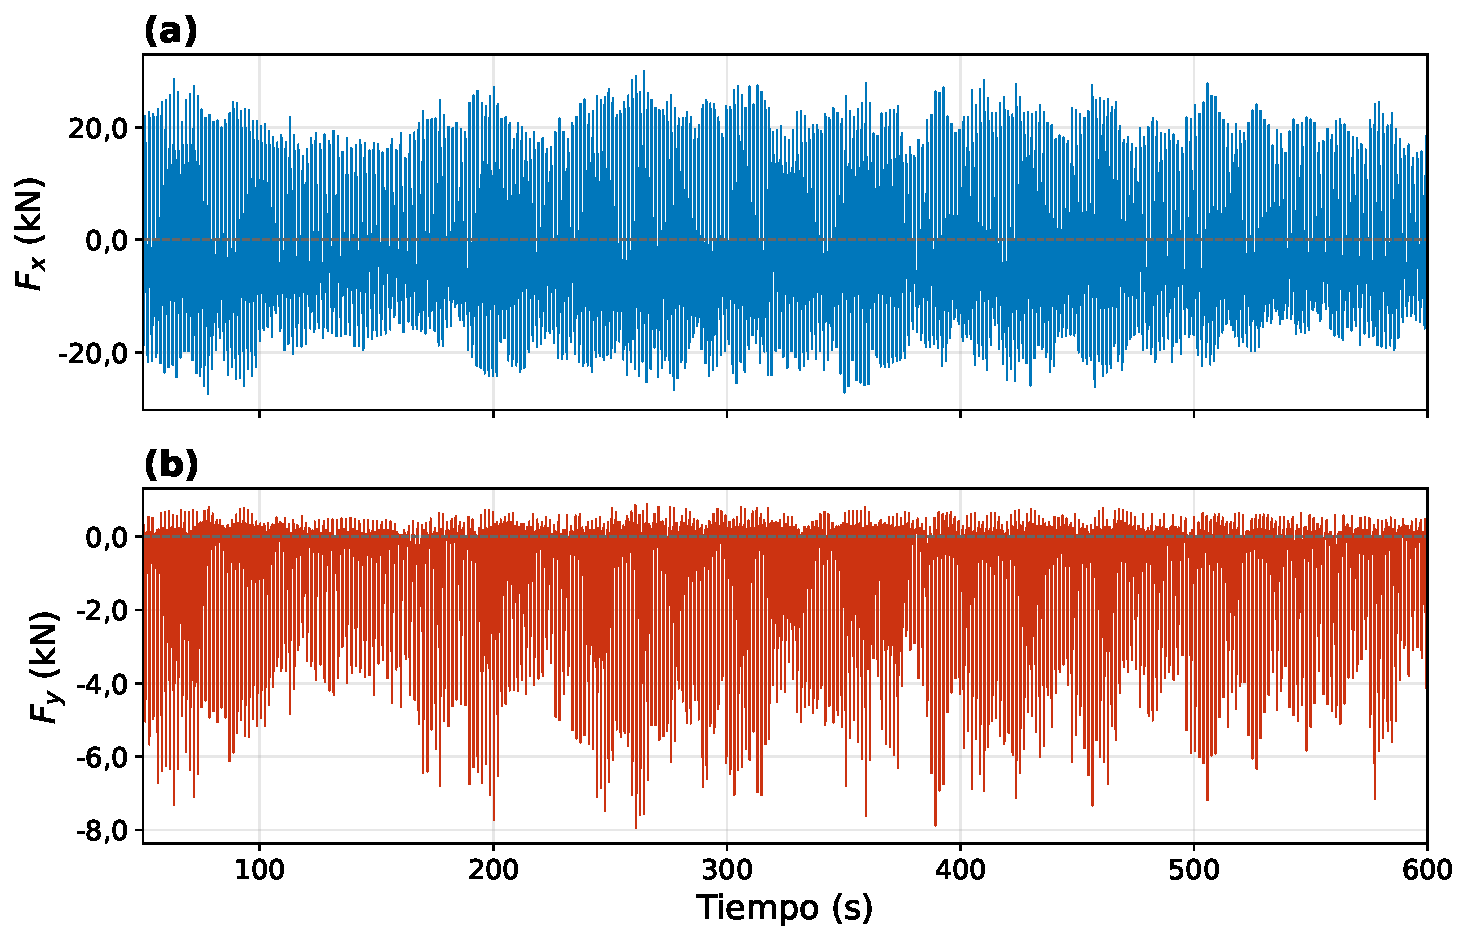
\includegraphics[width=0.85\textwidth]{Figuras/Figuras Anexo Fuerzas/fuerzas_xy_V10_S3.pdf}
    \caption{Fuerzas resultantes (a) $F_x$ y (b) $F_y$ en función del tiempo, $V = 10$~m/s, semilla $3$.}
    \label{fig:anexo_fuerzas_xy_V10_S3}
\end{figure}

\begin{figure}[H]
    \centering
    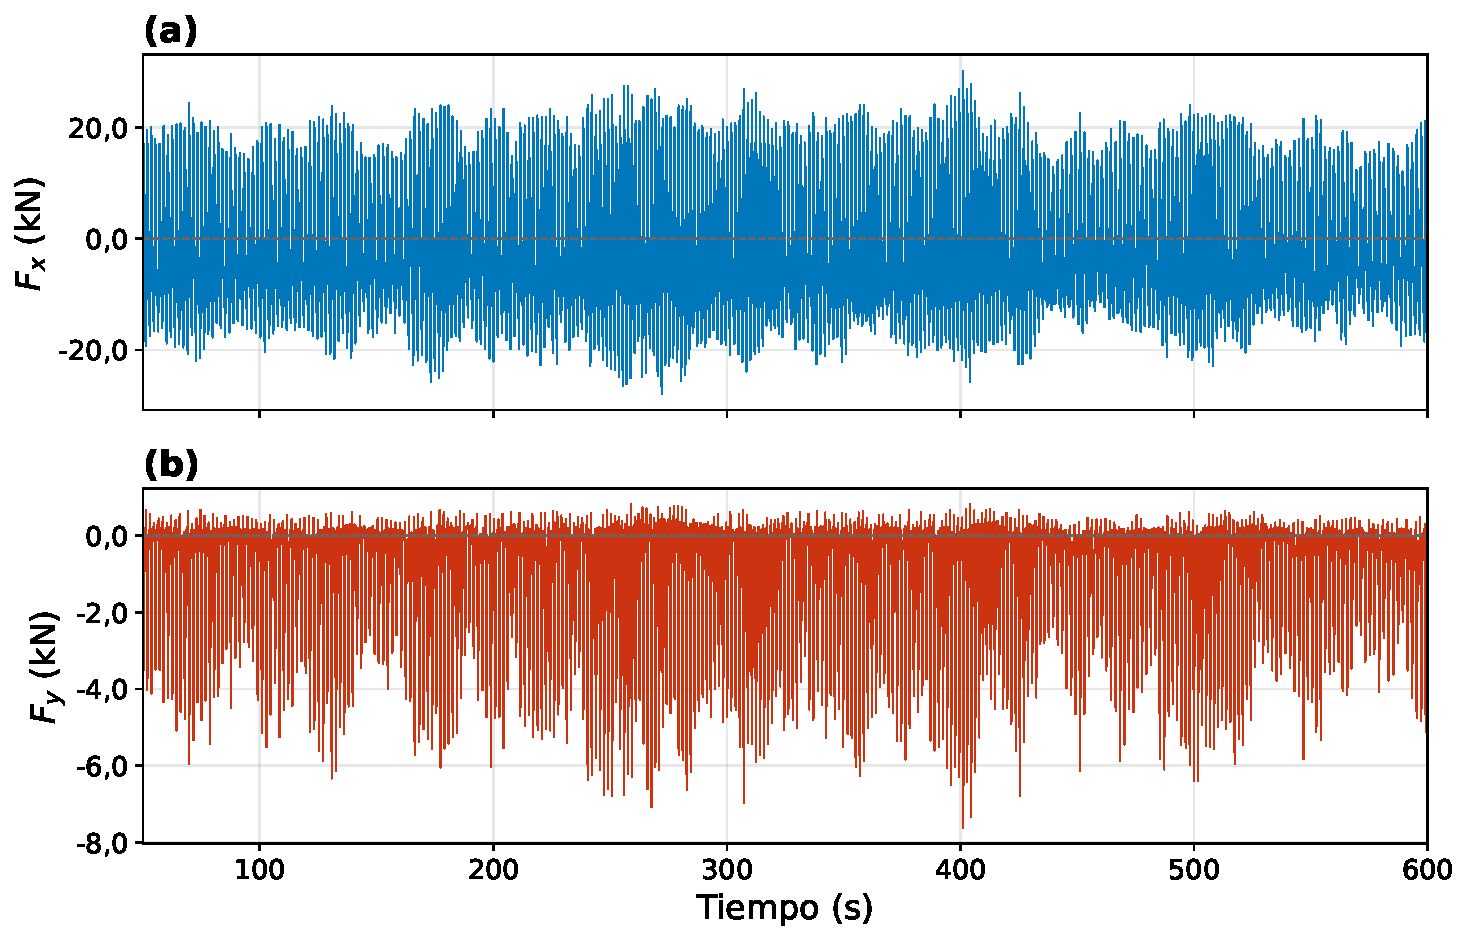
\includegraphics[width=0.85\textwidth]{Figuras/Figuras Anexo Fuerzas/fuerzas_xy_V10_S4.pdf}
    \caption{Fuerzas resultantes (a) $F_x$ y (b) $F_y$ en función del tiempo, $V = 10$~m/s, semilla $4$.}
    \label{fig:anexo_fuerzas_xy_V10_S4}
\end{figure}

\begin{figure}[H]
    \centering
    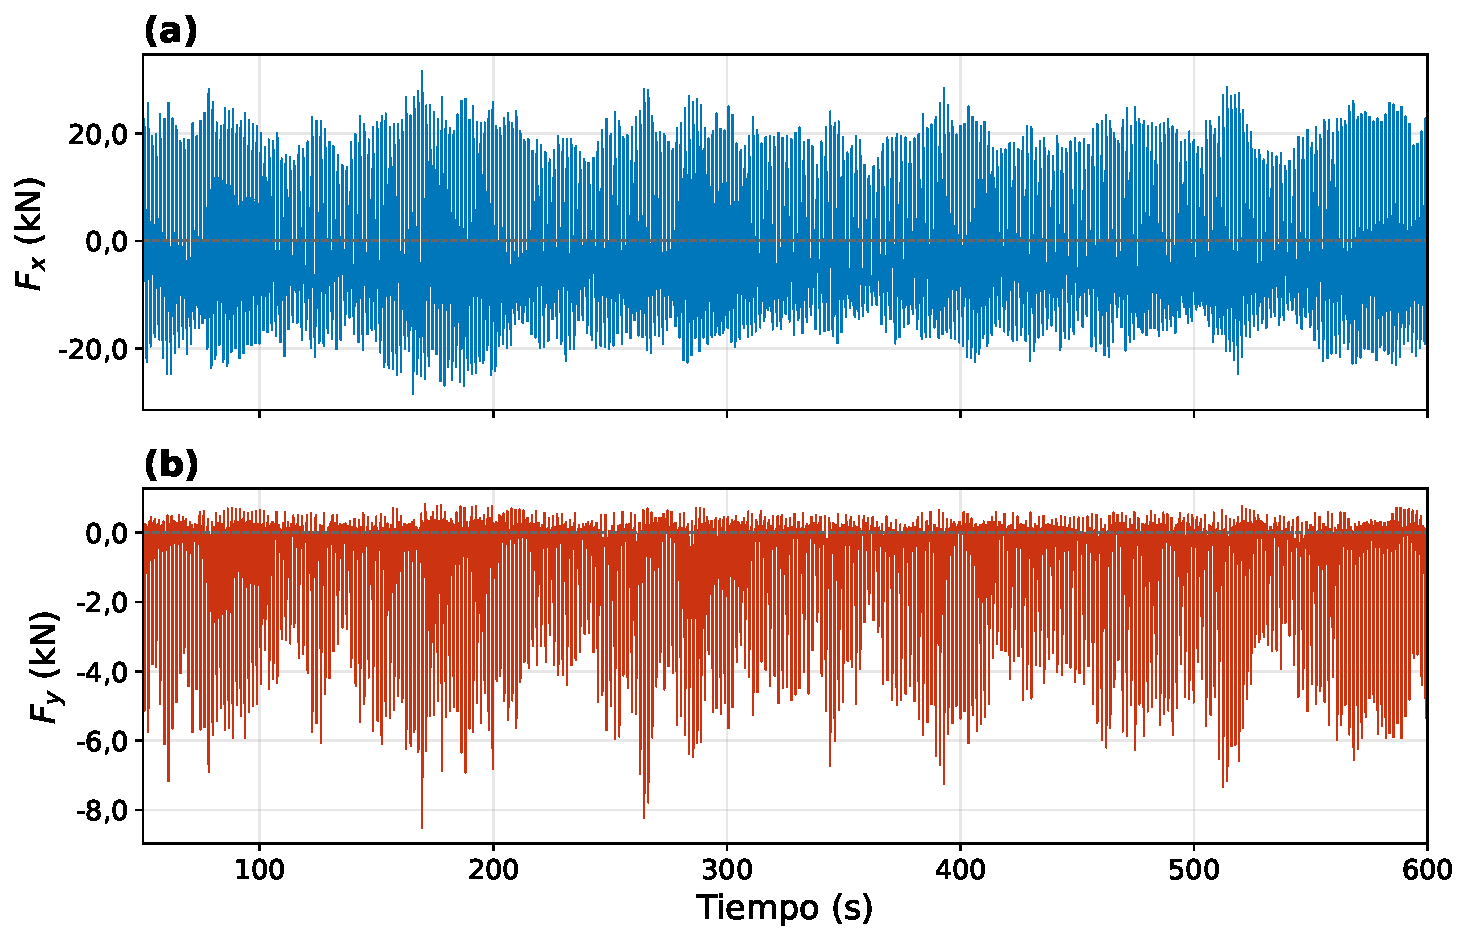
\includegraphics[width=0.85\textwidth]{Figuras/Figuras Anexo Fuerzas/fuerzas_xy_V10_S5.pdf}
    \caption{Fuerzas resultantes (a) $F_x$ y (b) $F_y$ en función del tiempo, $V = 10$~m/s, semilla $5$.}
    \label{fig:anexo_fuerzas_xy_V10_S5}
\end{figure}

\begin{figure}[H]
    \centering
    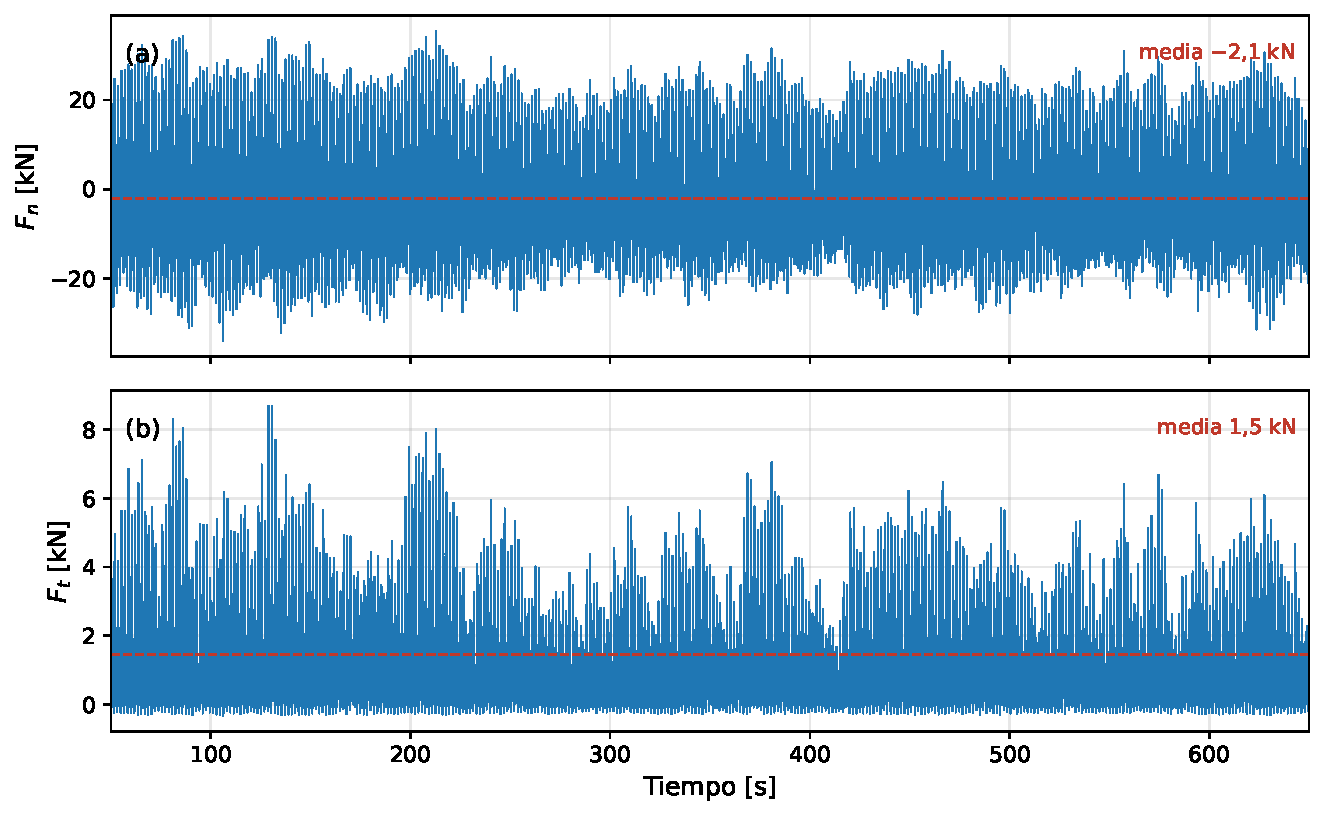
\includegraphics[width=0.85\textwidth]{Figuras/Figuras Anexo Fuerzas/fuerzas_xy_V10_S6.pdf}
    \caption{Fuerzas resultantes (a) $F_x$ y (b) $F_y$ en función del tiempo, $V = 10$~m/s, semilla $6$.}
    \label{fig:anexo_fuerzas_xy_V10_S6}
\end{figure}

\begin{figure}[H]
    \centering
    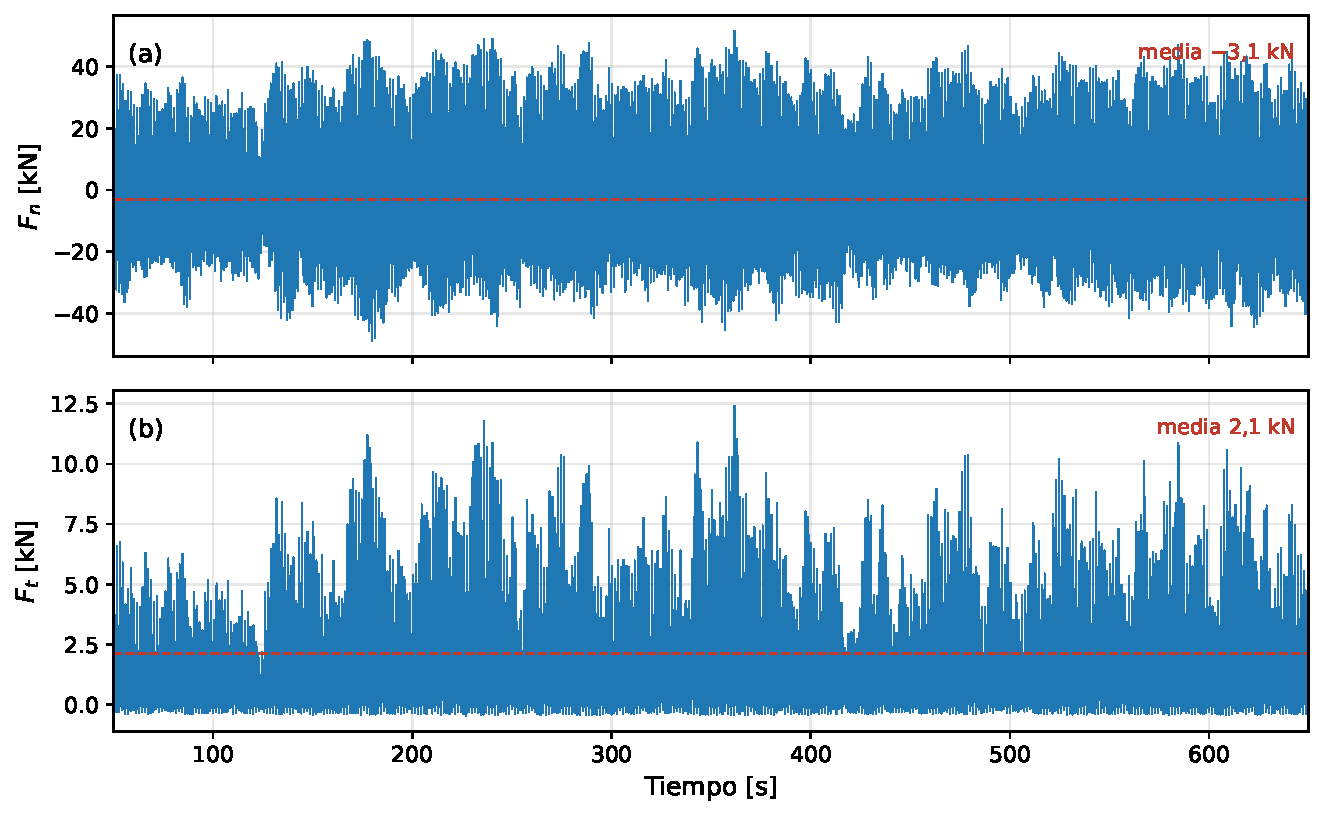
\includegraphics[width=0.85\textwidth]{Figuras/Figuras Anexo Fuerzas/fuerzas_xy_V12_S1.pdf}
    \caption{Fuerzas resultantes (a) $F_x$ y (b) $F_y$ en función del tiempo, $V = 12$~m/s, semilla $1$.}
    \label{fig:anexo_fuerzas_xy_V12_S1}
\end{figure}

\begin{figure}[H]
    \centering
    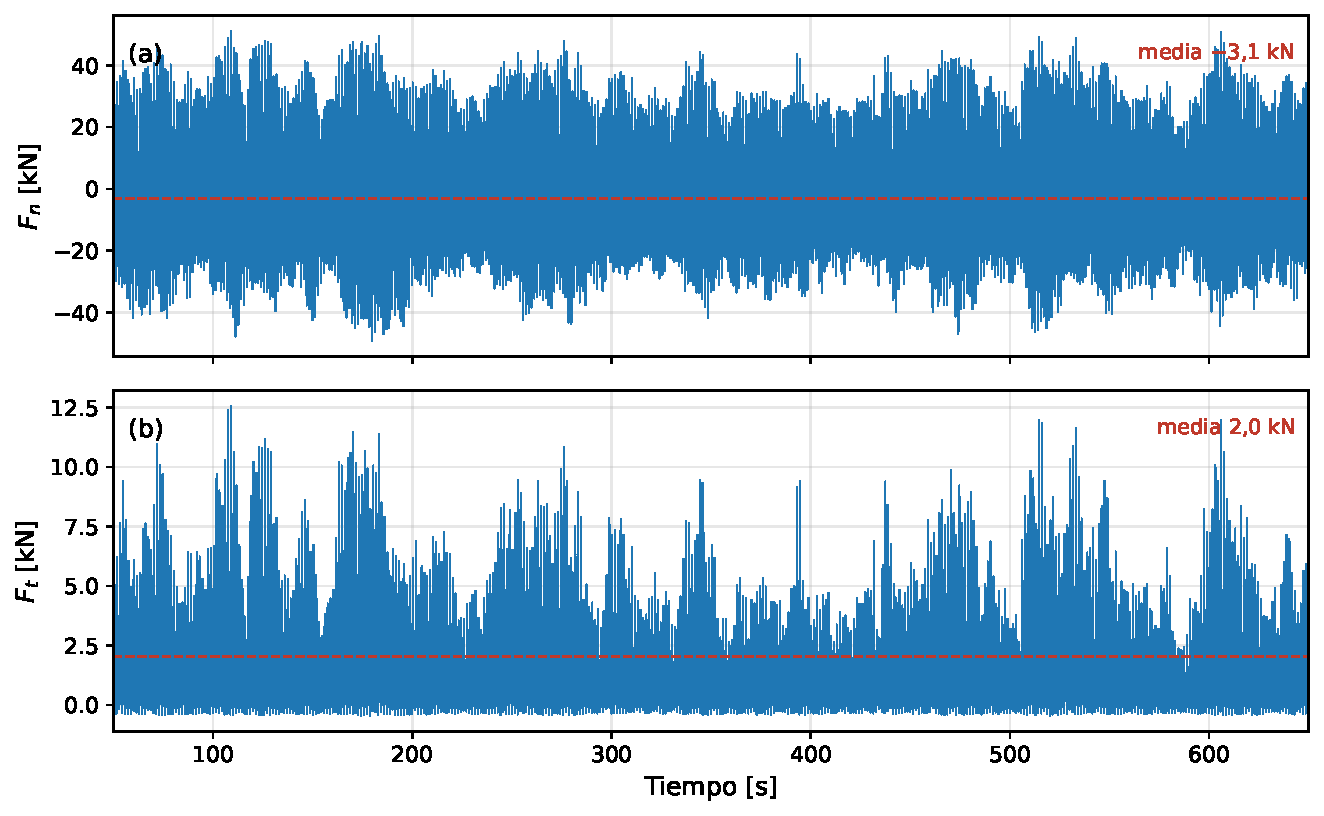
\includegraphics[width=0.85\textwidth]{Figuras/Figuras Anexo Fuerzas/fuerzas_xy_V12_S2.pdf}
    \caption{Fuerzas resultantes (a) $F_x$ y (b) $F_y$ en función del tiempo, $V = 12$~m/s, semilla $2$.}
    \label{fig:anexo_fuerzas_xy_V12_S2}
\end{figure}

\begin{figure}[H]
    \centering
    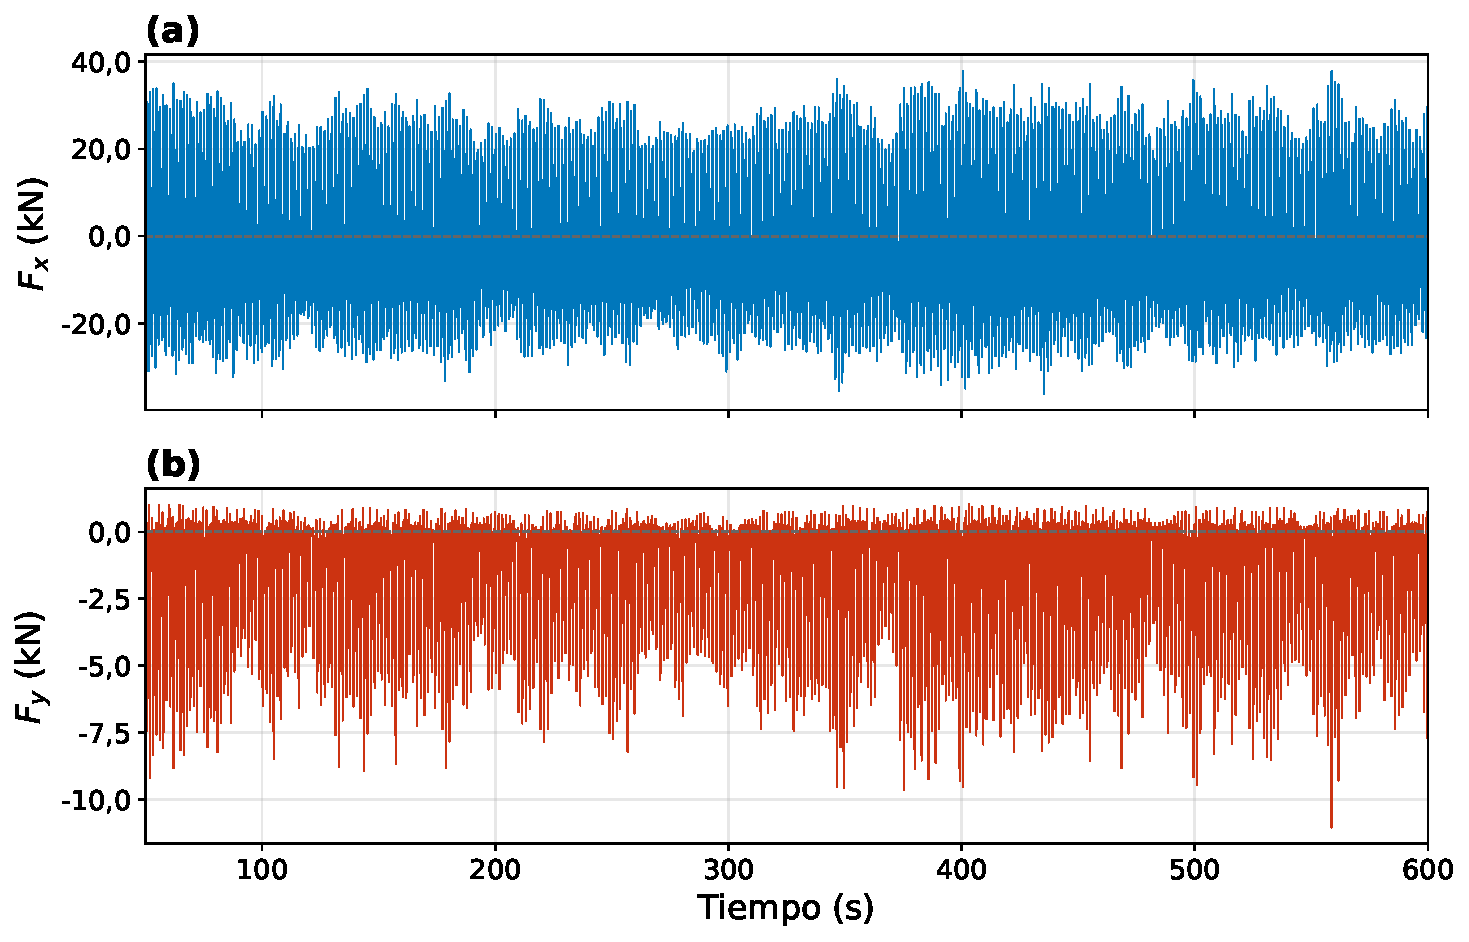
\includegraphics[width=0.85\textwidth]{Figuras/Figuras Anexo Fuerzas/fuerzas_xy_V12_S3.pdf}
    \caption{Fuerzas resultantes (a) $F_x$ y (b) $F_y$ en función del tiempo, $V = 12$~m/s, semilla $3$.}
    \label{fig:anexo_fuerzas_xy_V12_S3}
\end{figure}

\begin{figure}[H]
    \centering
    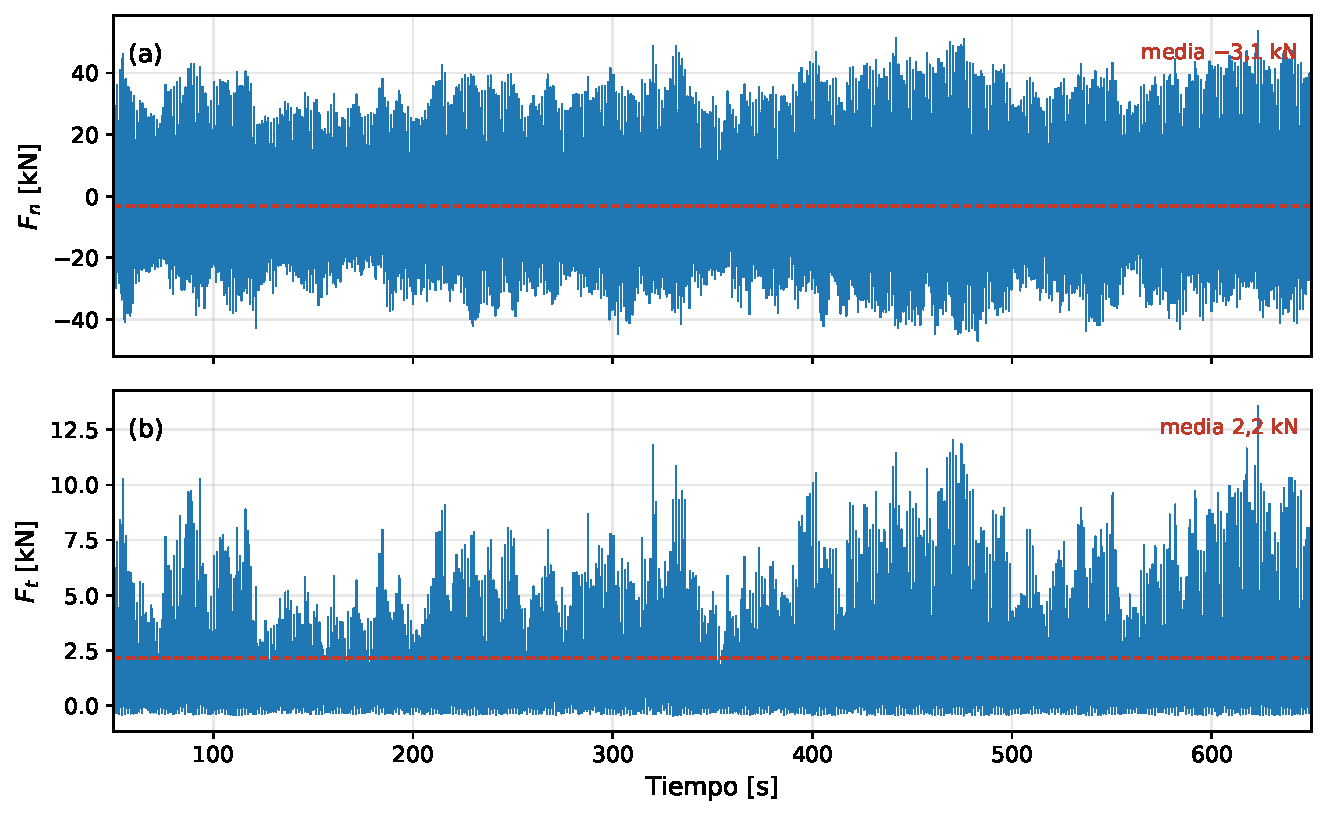
\includegraphics[width=0.85\textwidth]{Figuras/Figuras Anexo Fuerzas/fuerzas_xy_V12_S4.pdf}
    \caption{Fuerzas resultantes (a) $F_x$ y (b) $F_y$ en función del tiempo, $V = 12$~m/s, semilla $4$.}
    \label{fig:anexo_fuerzas_xy_V12_S4}
\end{figure}

\begin{figure}[H]
    \centering
    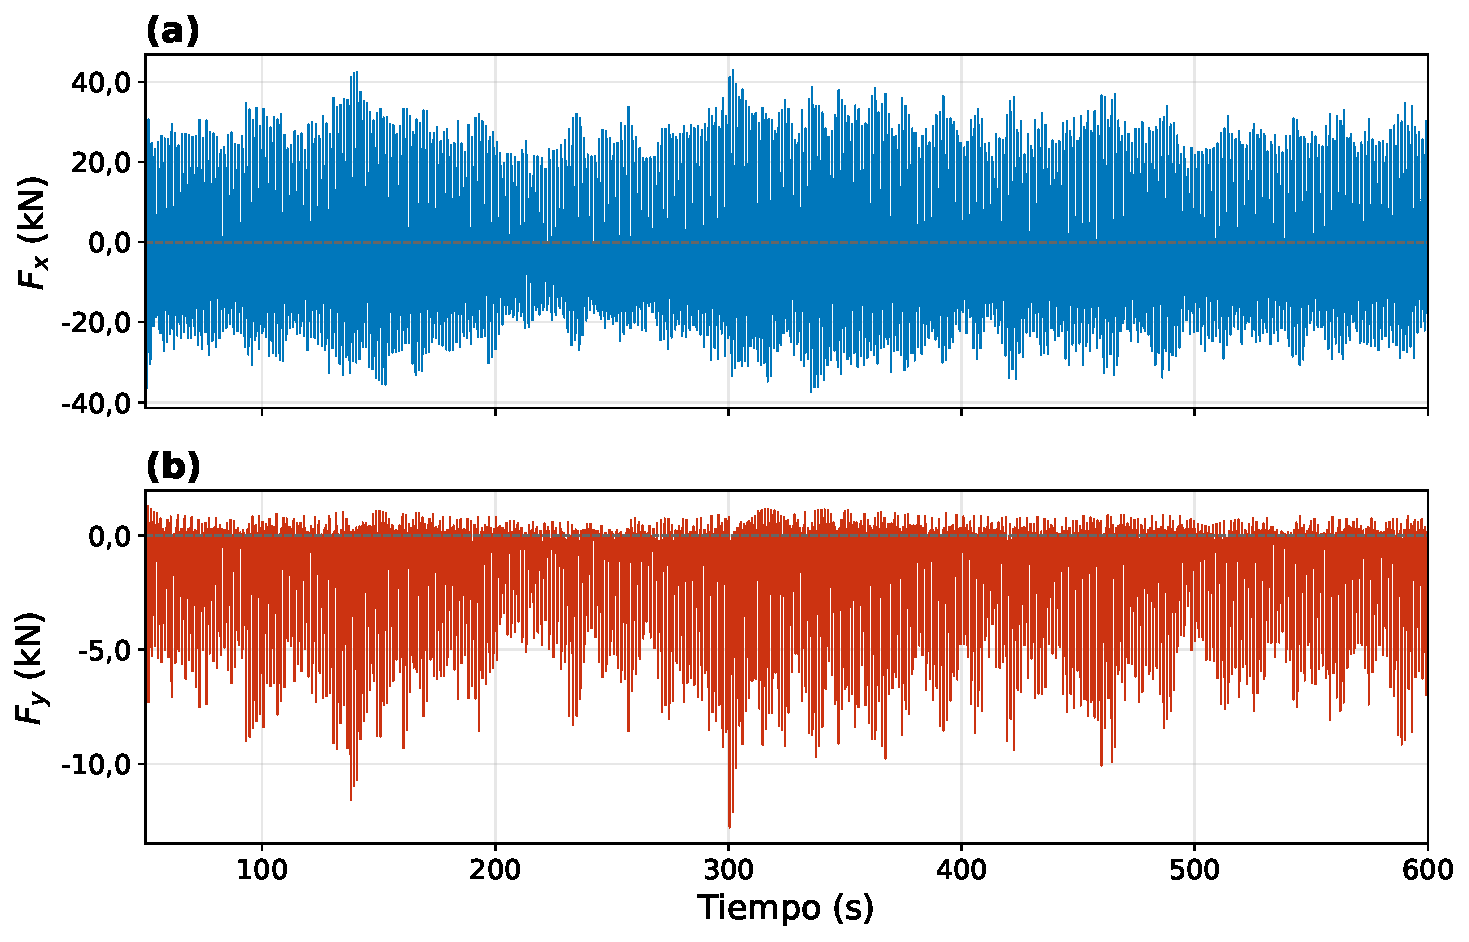
\includegraphics[width=0.85\textwidth]{Figuras/Figuras Anexo Fuerzas/fuerzas_xy_V12_S5.pdf}
    \caption{Fuerzas resultantes (a) $F_x$ y (b) $F_y$ en función del tiempo, $V = 12$~m/s, semilla $5$.}
    \label{fig:anexo_fuerzas_xy_V12_S5}
\end{figure}

\begin{figure}[H]
    \centering
    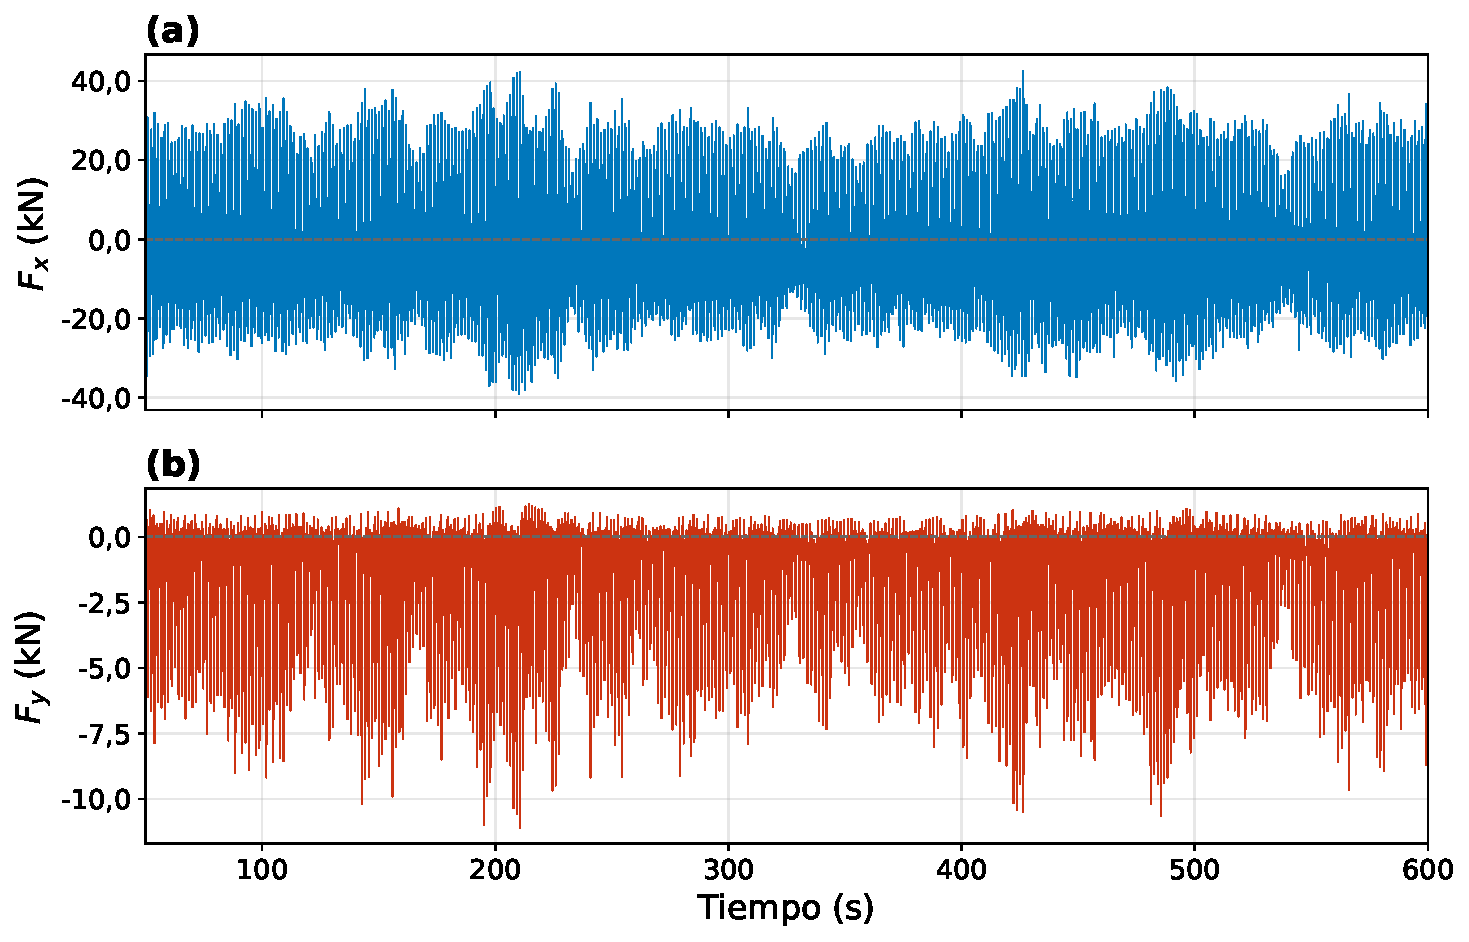
\includegraphics[width=0.85\textwidth]{Figuras/Figuras Anexo Fuerzas/fuerzas_xy_V12_S6.pdf}
    \caption{Fuerzas resultantes (a) $F_x$ y (b) $F_y$ en función del tiempo, $V = 12$~m/s, semilla $6$.}
    \label{fig:anexo_fuerzas_xy_V12_S6}
\end{figure}

\begin{figure}[H]
    \centering
    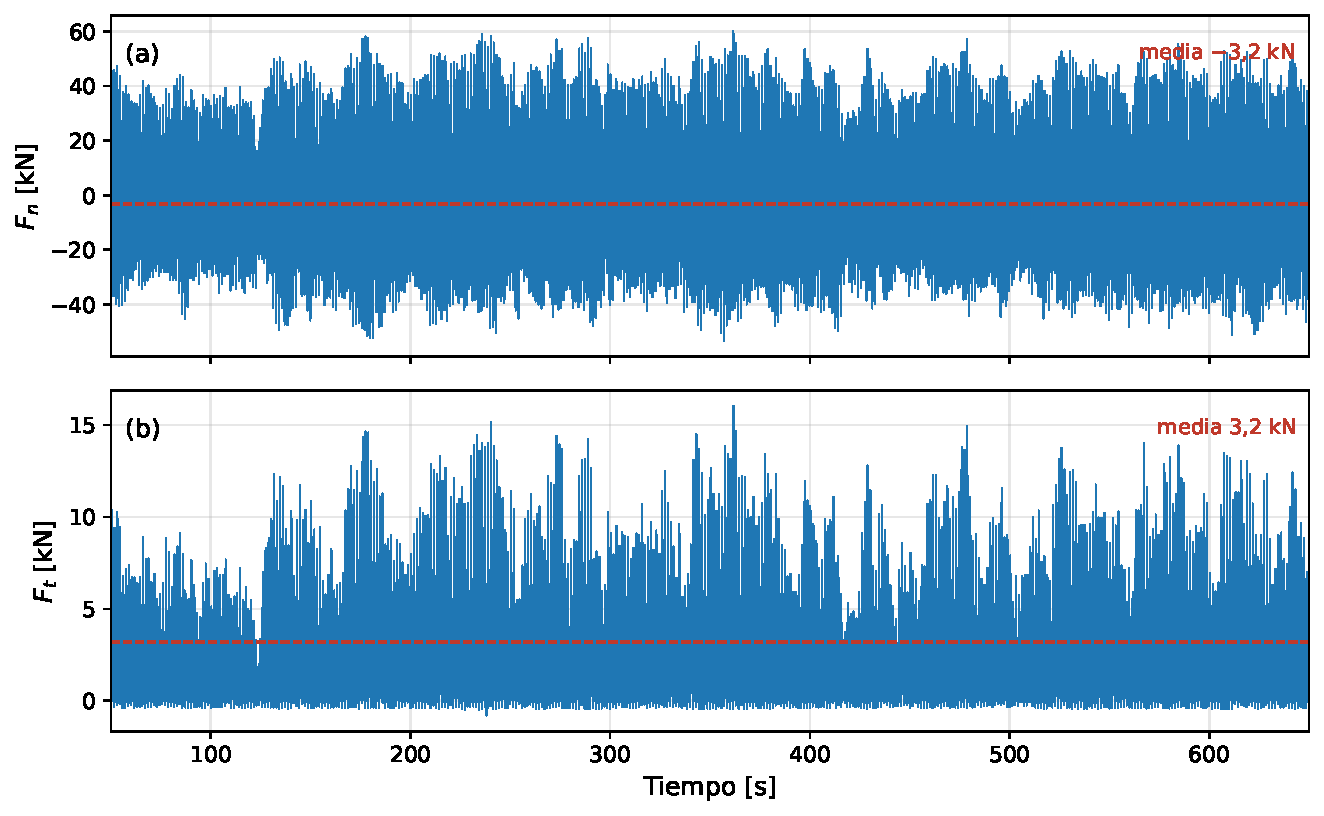
\includegraphics[width=0.85\textwidth]{Figuras/Figuras Anexo Fuerzas/fuerzas_xy_V14_S1.pdf}
    \caption{Fuerzas resultantes (a) $F_x$ y (b) $F_y$ en función del tiempo, $V = 14$~m/s, semilla $1$.}
    \label{fig:anexo_fuerzas_xy_V14_S1}
\end{figure}

\begin{figure}[H]
    \centering
    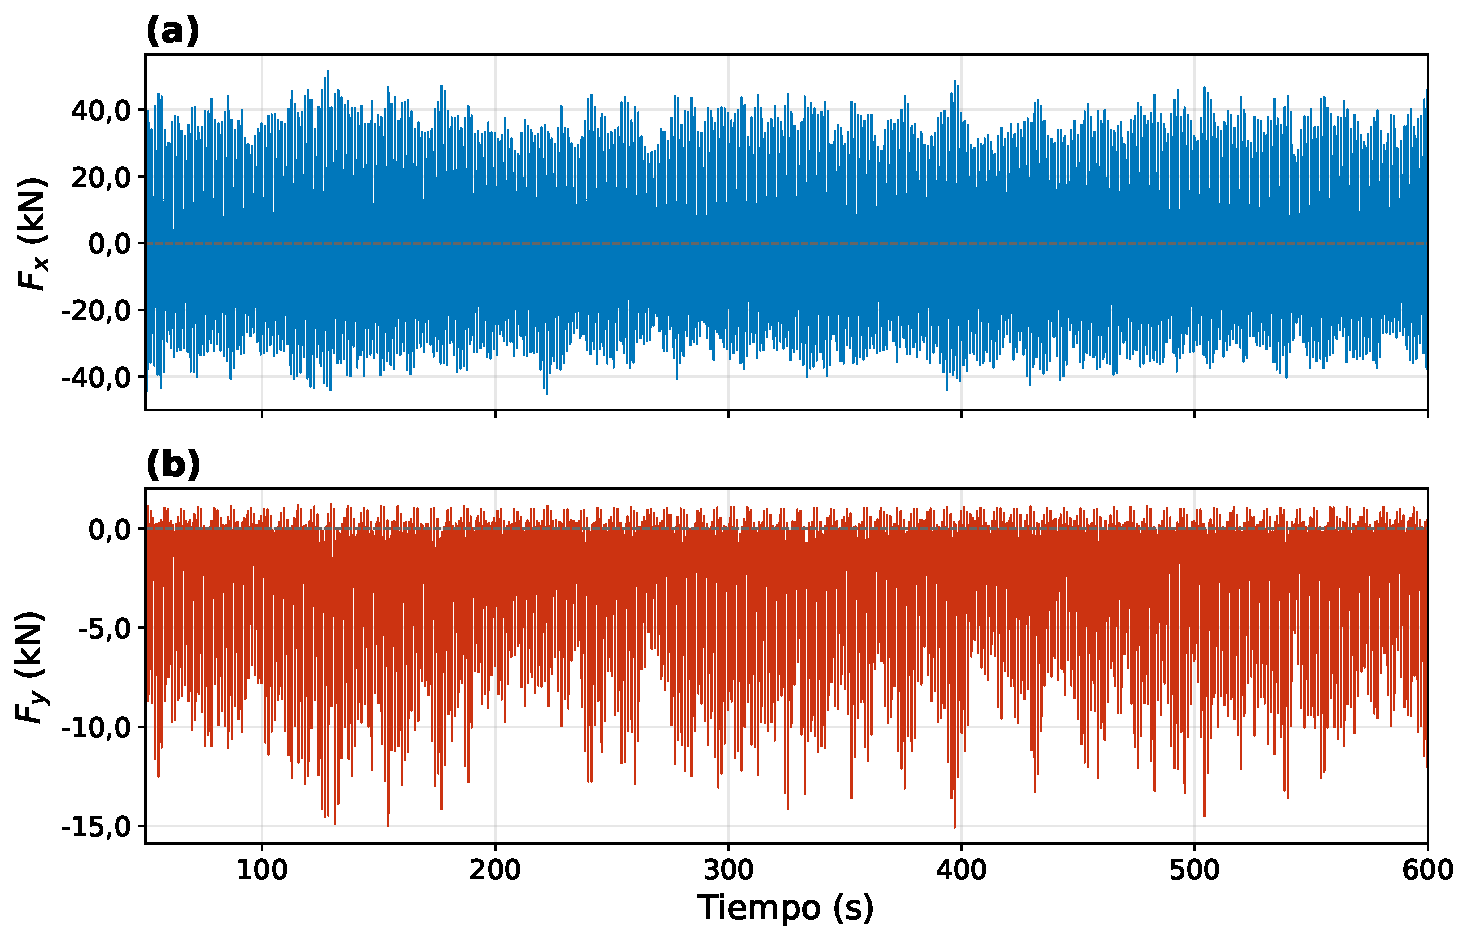
\includegraphics[width=0.85\textwidth]{Figuras/Figuras Anexo Fuerzas/fuerzas_xy_V14_S2.pdf}
    \caption{Fuerzas resultantes (a) $F_x$ y (b) $F_y$ en función del tiempo, $V = 14$~m/s, semilla $2$.}
    \label{fig:anexo_fuerzas_xy_V14_S2}
\end{figure}

\begin{figure}[H]
    \centering
    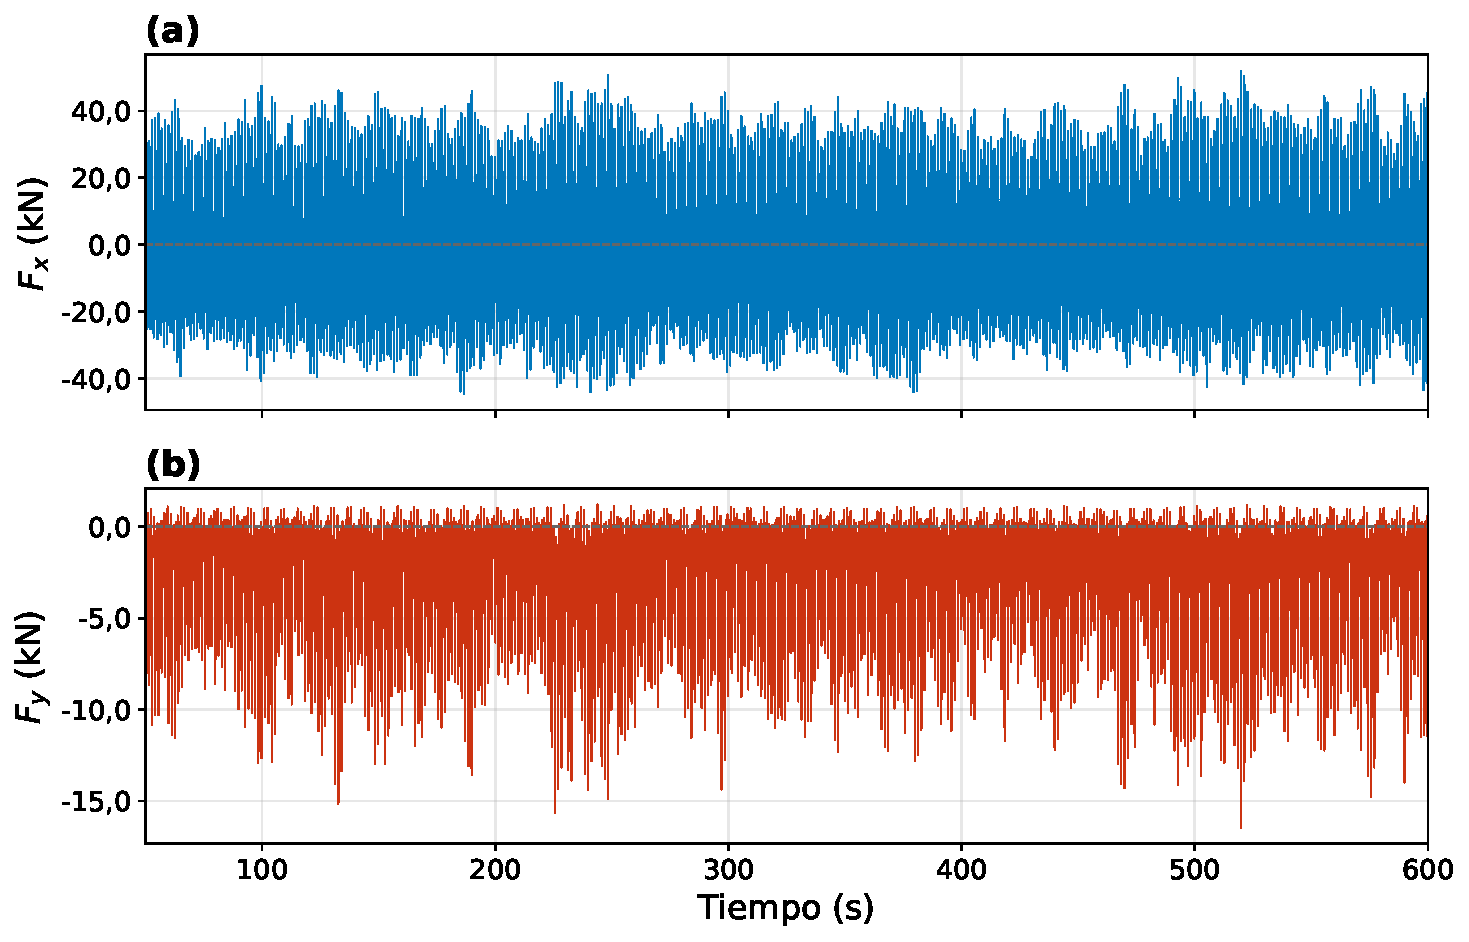
\includegraphics[width=0.85\textwidth]{Figuras/Figuras Anexo Fuerzas/fuerzas_xy_V14_S3.pdf}
    \caption{Fuerzas resultantes (a) $F_x$ y (b) $F_y$ en función del tiempo, $V = 14$~m/s, semilla $3$.}
    \label{fig:anexo_fuerzas_xy_V14_S3}
\end{figure}

\begin{figure}[H]
    \centering
    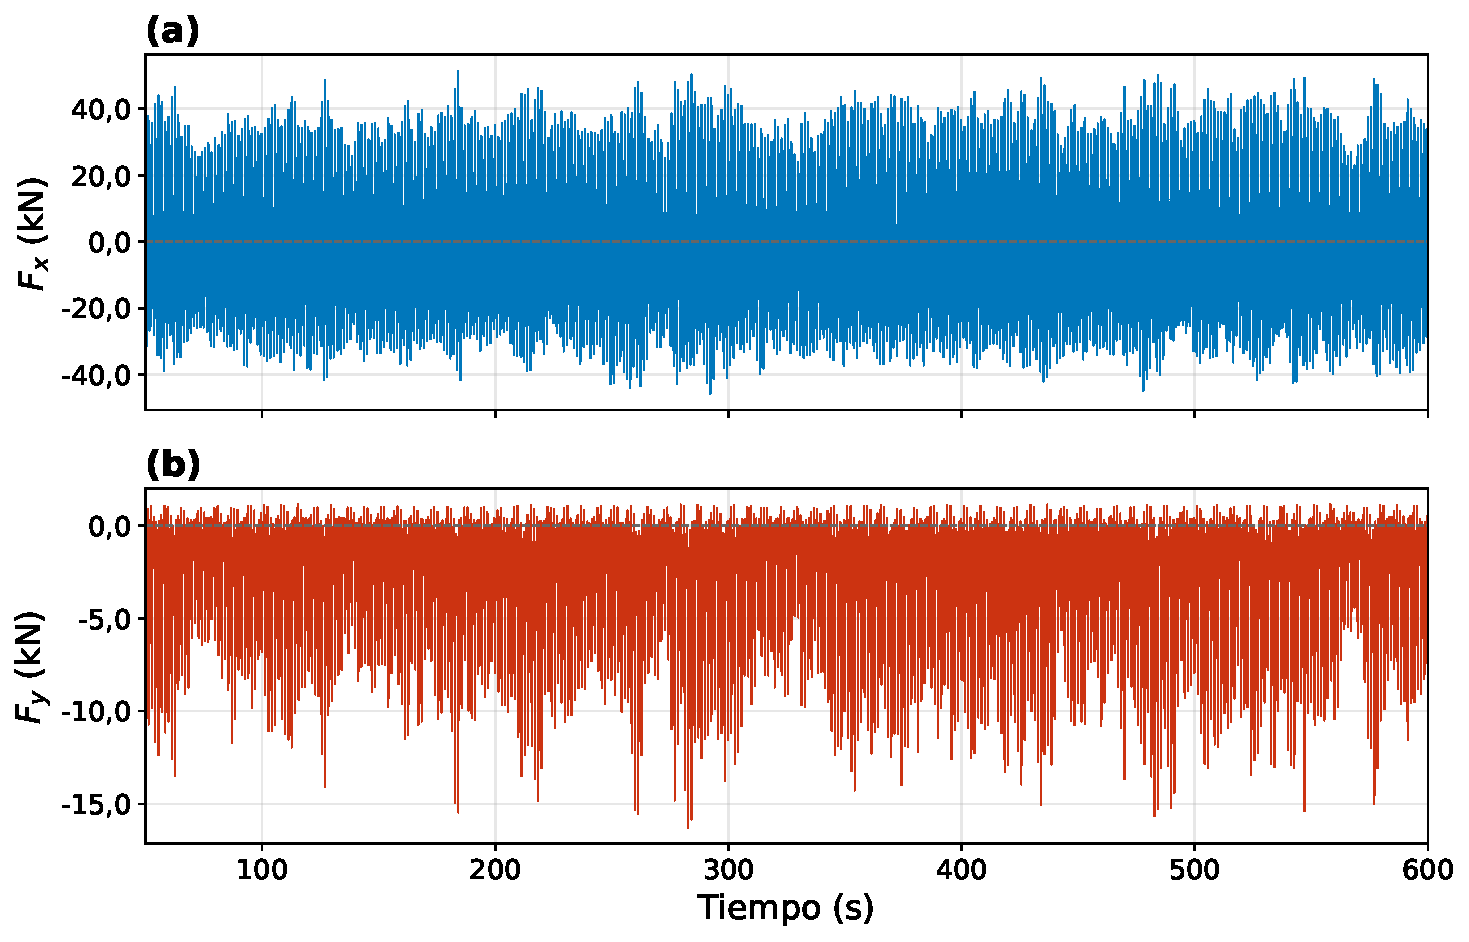
\includegraphics[width=0.85\textwidth]{Figuras/Figuras Anexo Fuerzas/fuerzas_xy_V14_S4.pdf}
    \caption{Fuerzas resultantes (a) $F_x$ y (b) $F_y$ en función del tiempo, $V = 14$~m/s, semilla $4$.}
    \label{fig:anexo_fuerzas_xy_V14_S4}
\end{figure}

\begin{figure}[H]
    \centering
    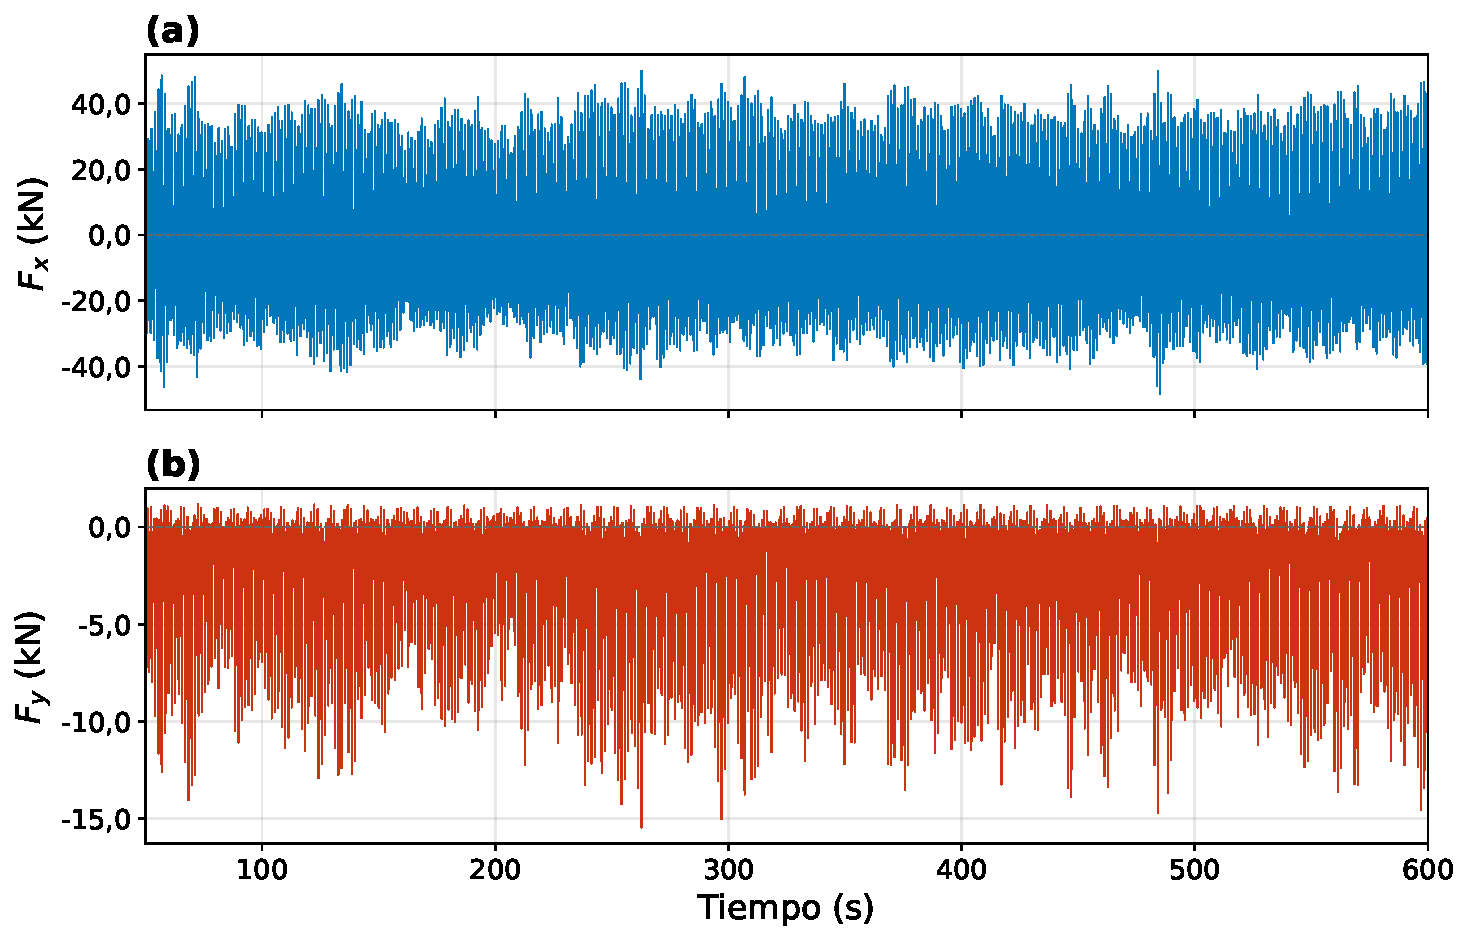
\includegraphics[width=0.85\textwidth]{Figuras/Figuras Anexo Fuerzas/fuerzas_xy_V14_S5.pdf}
    \caption{Fuerzas resultantes (a) $F_x$ y (b) $F_y$ en función del tiempo, $V = 14$~m/s, semilla $5$.}
    \label{fig:anexo_fuerzas_xy_V14_S5}
\end{figure}

\begin{figure}[H]
    \centering
    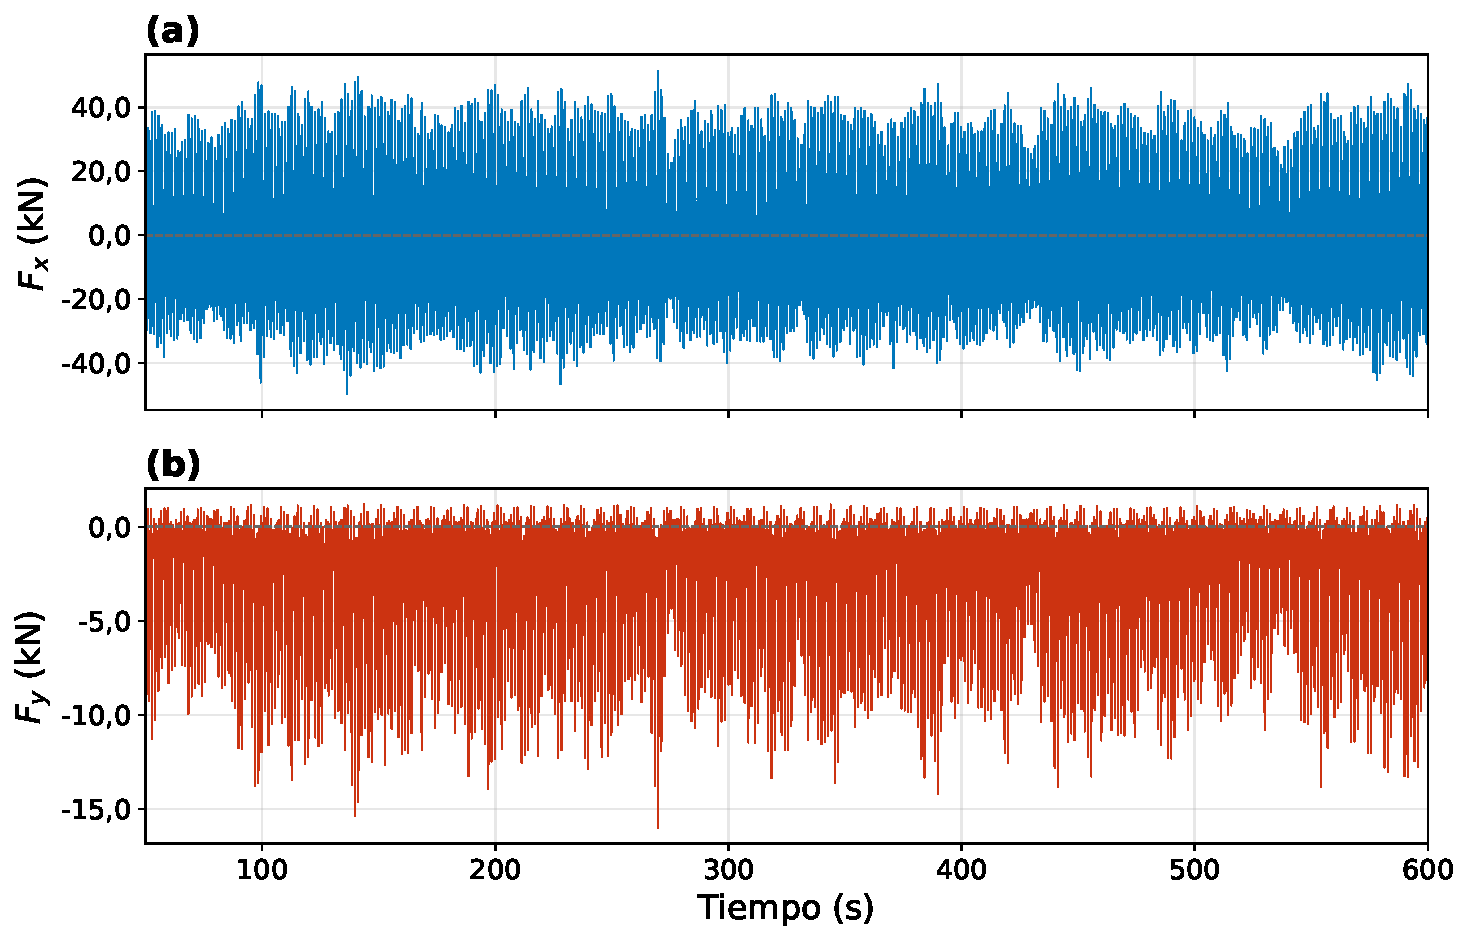
\includegraphics[width=0.85\textwidth]{Figuras/Figuras Anexo Fuerzas/fuerzas_xy_V14_S6.pdf}
    \caption{Fuerzas resultantes (a) $F_x$ y (b) $F_y$ en función del tiempo, $V = 14$~m/s, semilla $6$.}
    \label{fig:anexo_fuerzas_xy_V14_S6}
\end{figure}

\begin{figure}[H]
    \centering
    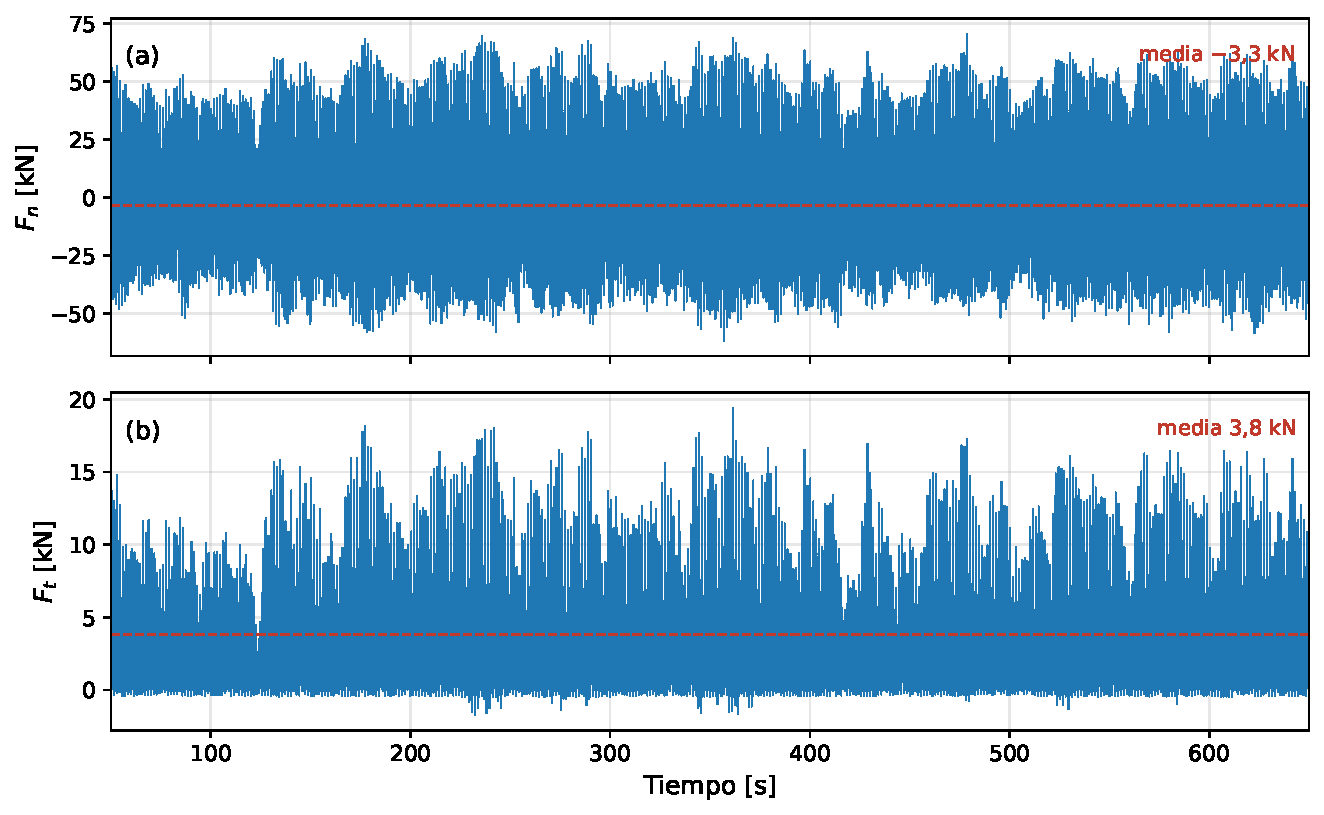
\includegraphics[width=0.85\textwidth]{Figuras/Figuras Anexo Fuerzas/fuerzas_xy_V16_S1.pdf}
    \caption{Fuerzas resultantes (a) $F_x$ y (b) $F_y$ en función del tiempo, $V = 16$~m/s, semilla $1$.}
    \label{fig:anexo_fuerzas_xy_V16_S1}
\end{figure}

\begin{figure}[H]
    \centering
    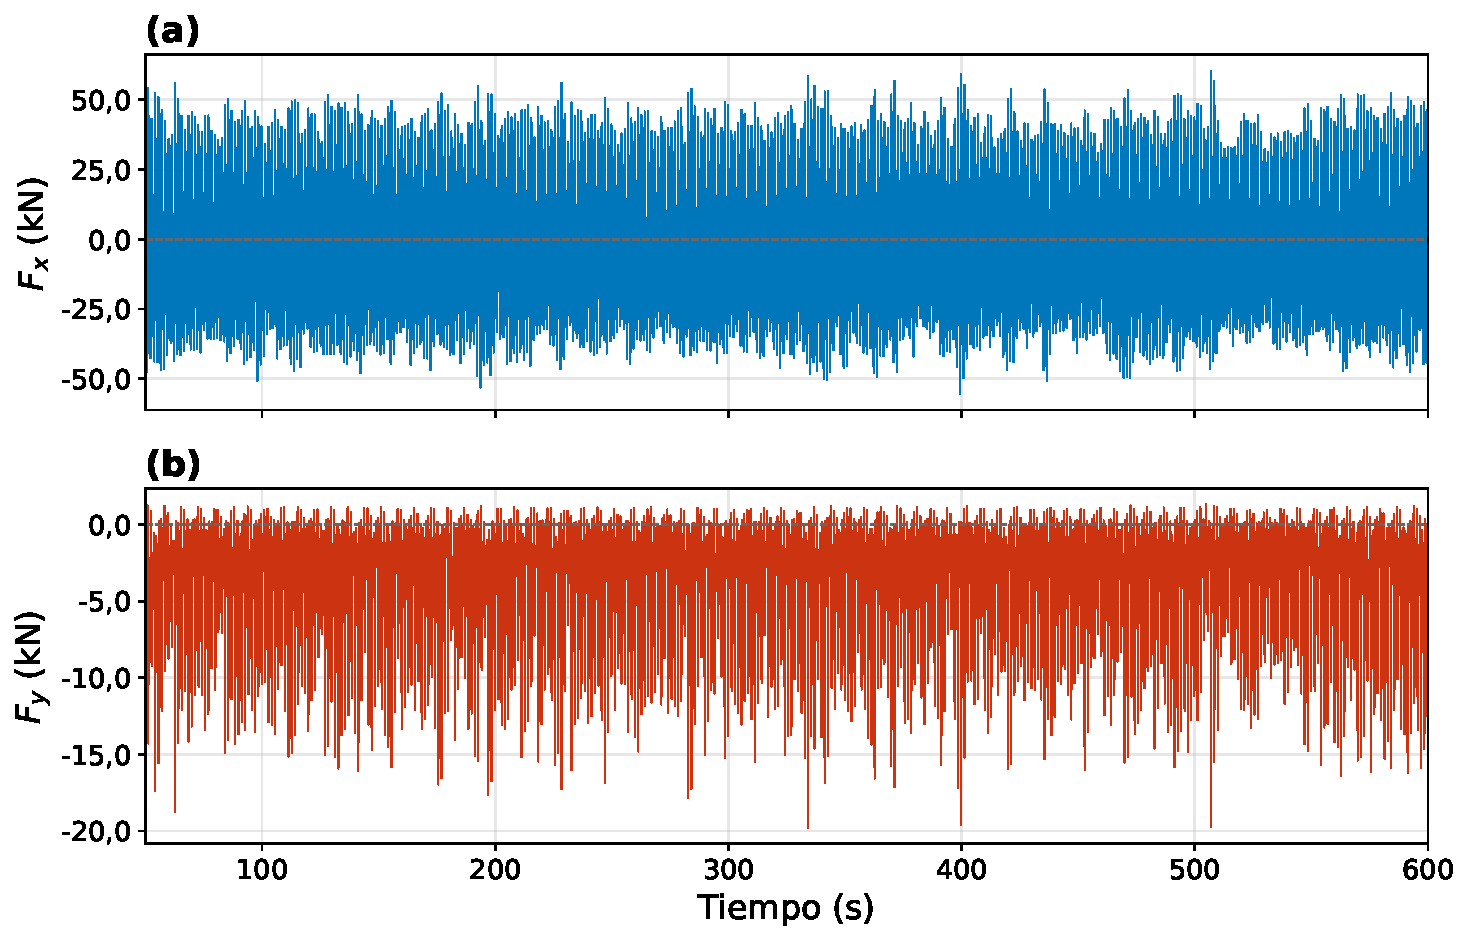
\includegraphics[width=0.85\textwidth]{Figuras/Figuras Anexo Fuerzas/fuerzas_xy_V16_S2.pdf}
    \caption{Fuerzas resultantes (a) $F_x$ y (b) $F_y$ en función del tiempo, $V = 16$~m/s, semilla $2$.}
    \label{fig:anexo_fuerzas_xy_V16_S2}
\end{figure}

\begin{figure}[H]
    \centering
    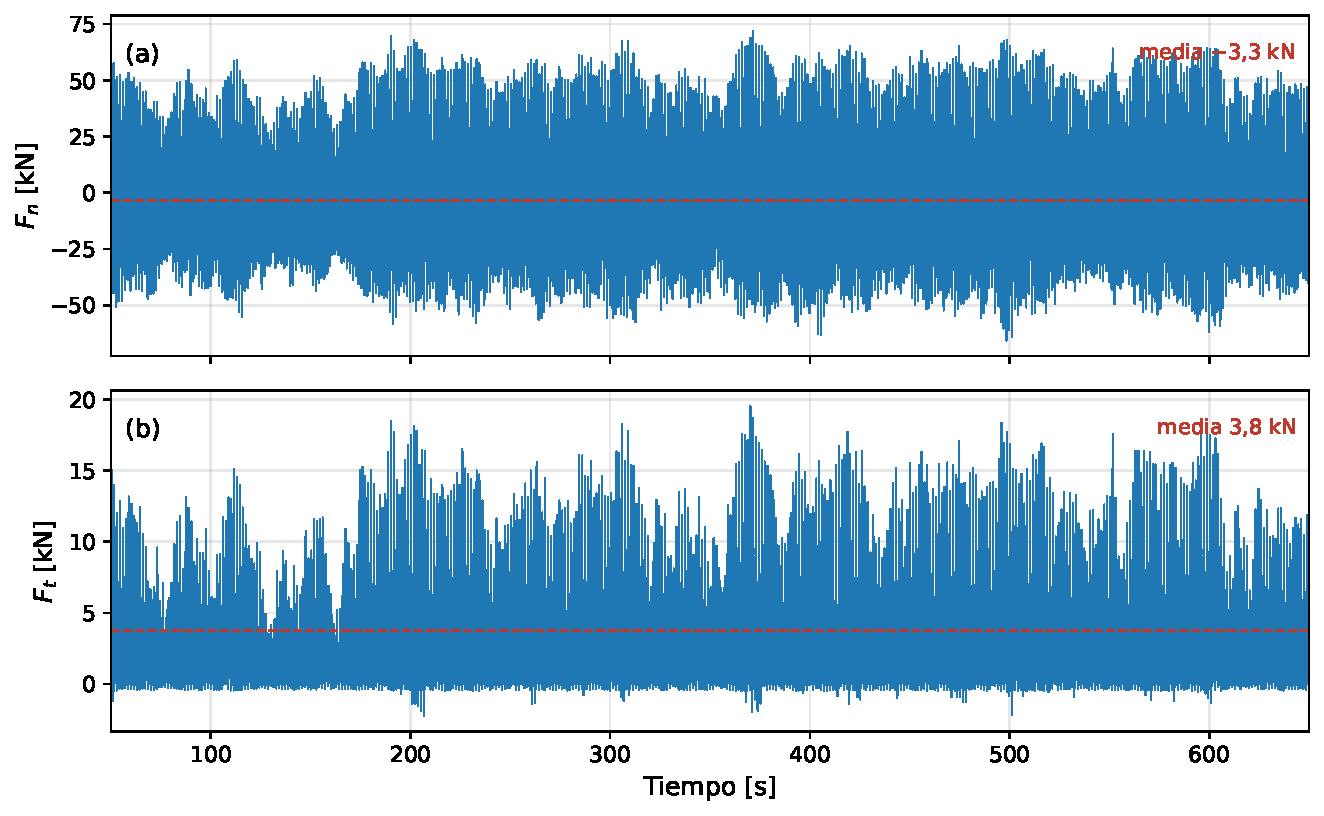
\includegraphics[width=0.85\textwidth]{Figuras/Figuras Anexo Fuerzas/fuerzas_xy_V16_S3.pdf}
    \caption{Fuerzas resultantes (a) $F_x$ y (b) $F_y$ en función del tiempo, $V = 16$~m/s, semilla $3$.}
    \label{fig:anexo_fuerzas_xy_V16_S3}
\end{figure}

\begin{figure}[H]
    \centering
    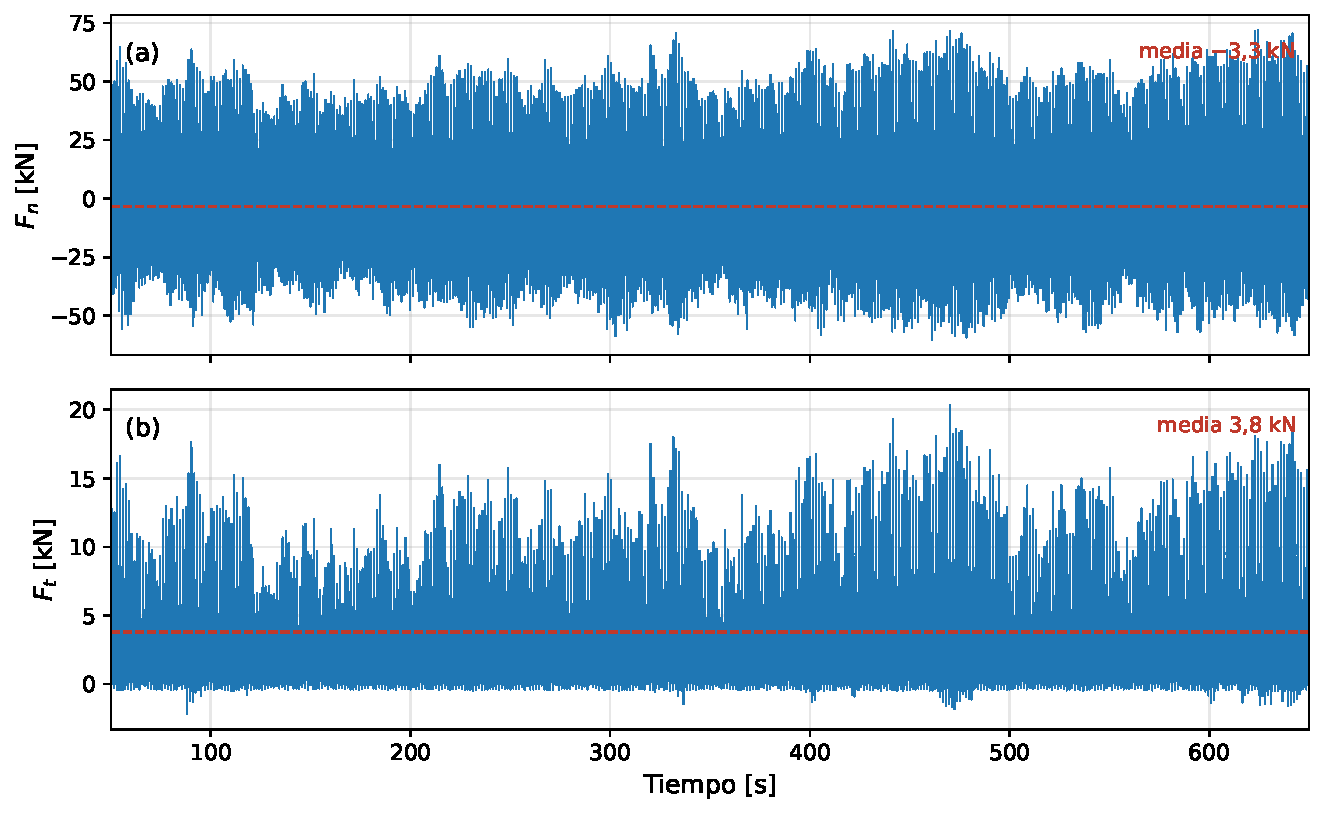
\includegraphics[width=0.85\textwidth]{Figuras/Figuras Anexo Fuerzas/fuerzas_xy_V16_S4.pdf}
    \caption{Fuerzas resultantes (a) $F_x$ y (b) $F_y$ en función del tiempo, $V = 16$~m/s, semilla $4$.}
    \label{fig:anexo_fuerzas_xy_V16_S4}
\end{figure}

\begin{figure}[H]
    \centering
    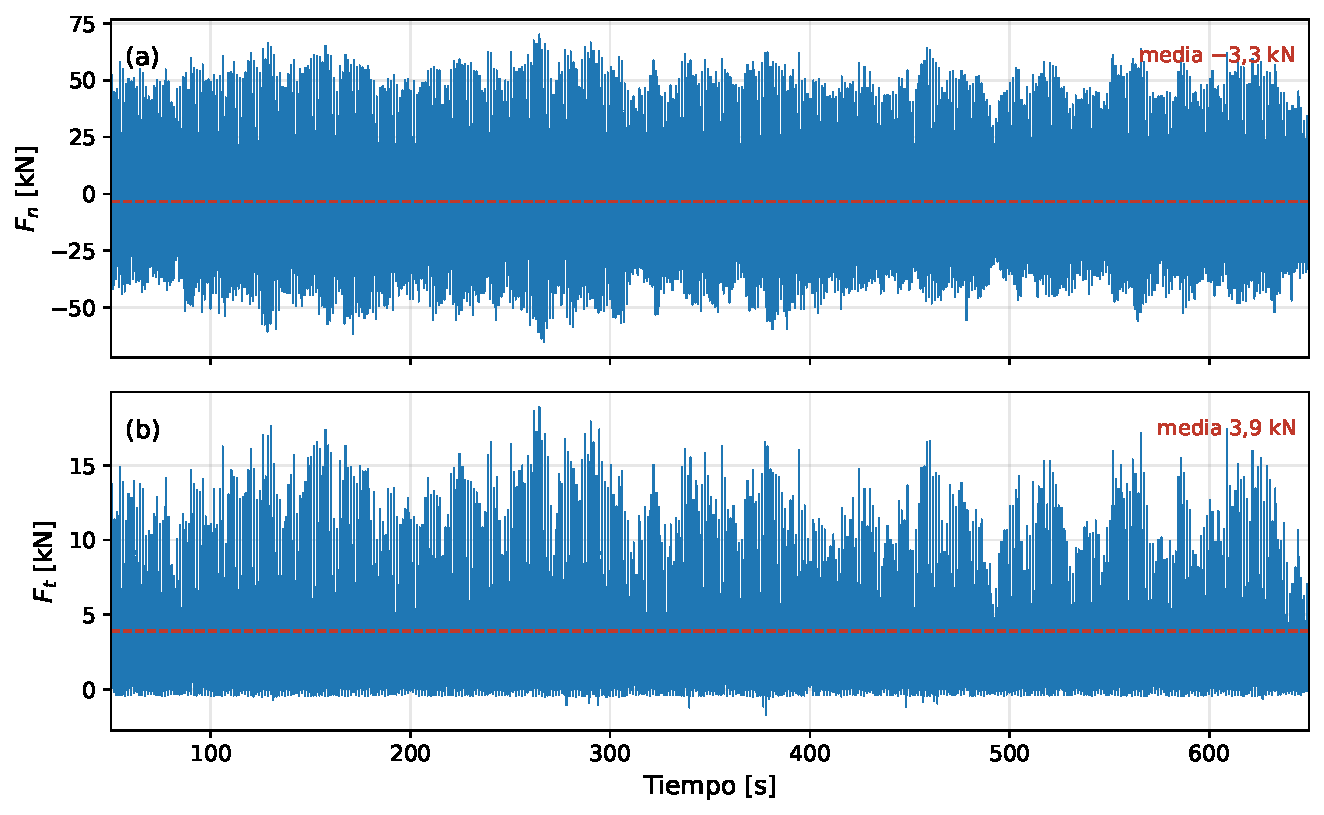
\includegraphics[width=0.85\textwidth]{Figuras/Figuras Anexo Fuerzas/fuerzas_xy_V16_S5.pdf}
    \caption{Fuerzas resultantes (a) $F_x$ y (b) $F_y$ en función del tiempo, $V = 16$~m/s, semilla $5$.}
    \label{fig:anexo_fuerzas_xy_V16_S5}
\end{figure}

\begin{figure}[H]
    \centering
    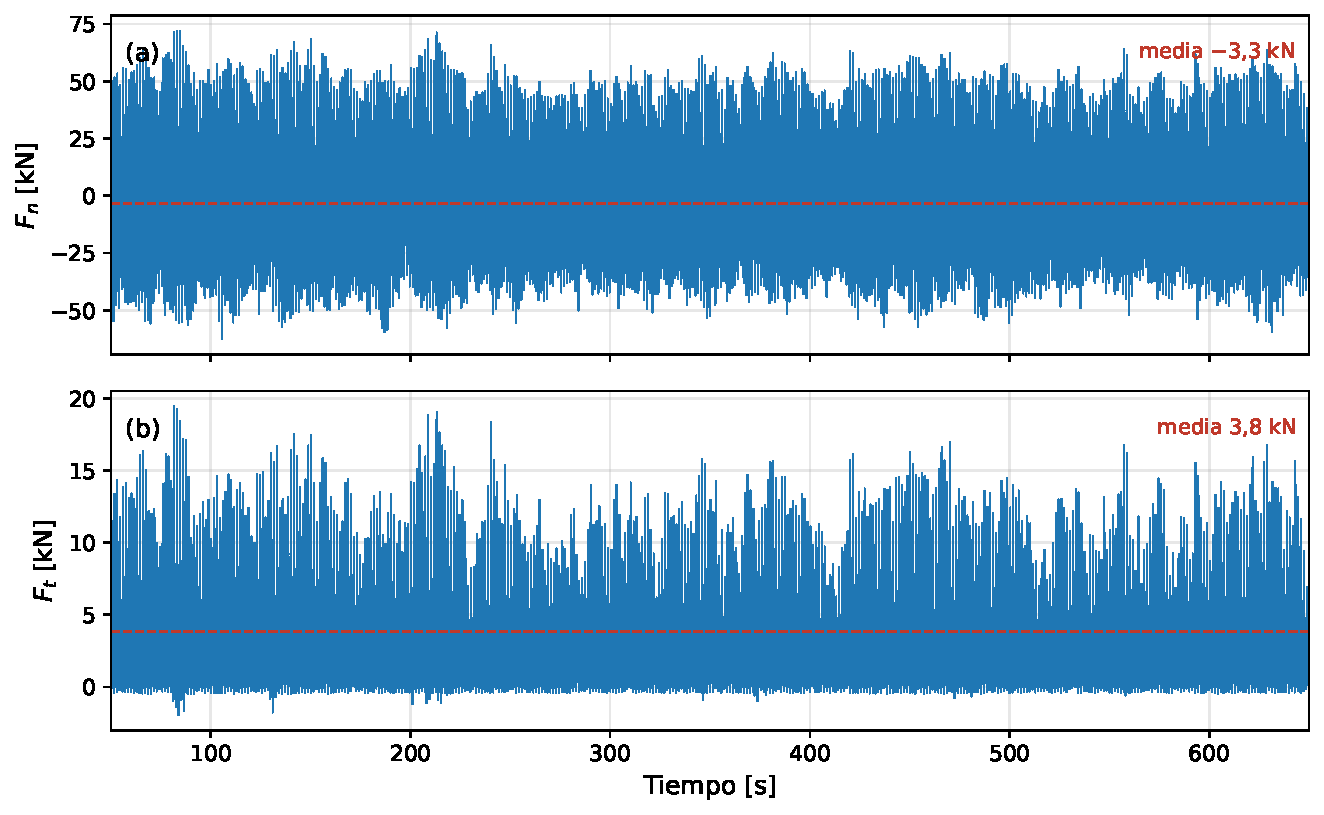
\includegraphics[width=0.85\textwidth]{Figuras/Figuras Anexo Fuerzas/fuerzas_xy_V16_S6.pdf}
    \caption{Fuerzas resultantes (a) $F_x$ y (b) $F_y$ en función del tiempo, $V = 16$~m/s, semilla $6$.}
    \label{fig:anexo_fuerzas_xy_V16_S6}
\end{figure}

\begin{figure}[H]
    \centering
    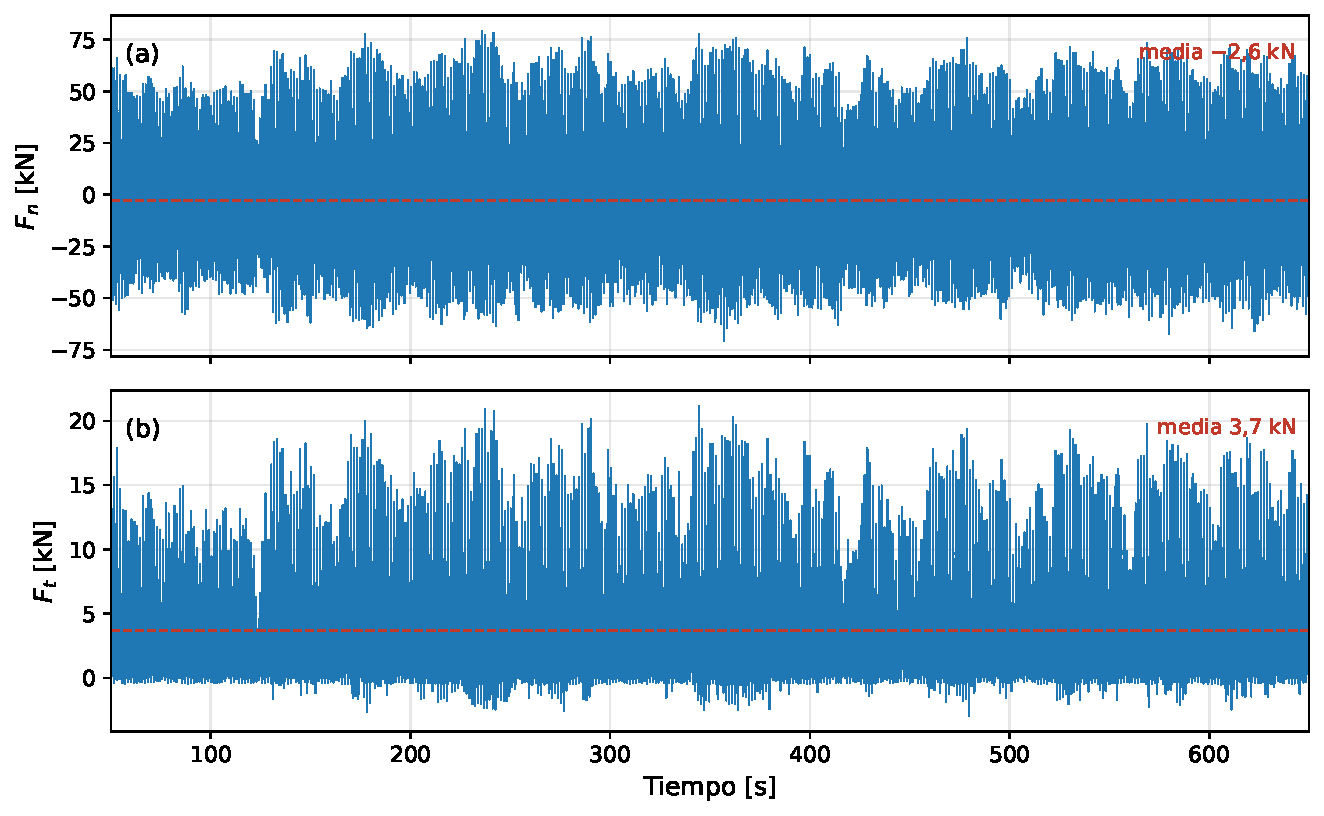
\includegraphics[width=0.85\textwidth]{Figuras/Figuras Anexo Fuerzas/fuerzas_xy_V18_S1.pdf}
    \caption{Fuerzas resultantes (a) $F_x$ y (b) $F_y$ en función del tiempo, $V = 18$~m/s, semilla $1$.}
    \label{fig:anexo_fuerzas_xy_V18_S1}
\end{figure}

\begin{figure}[H]
    \centering
    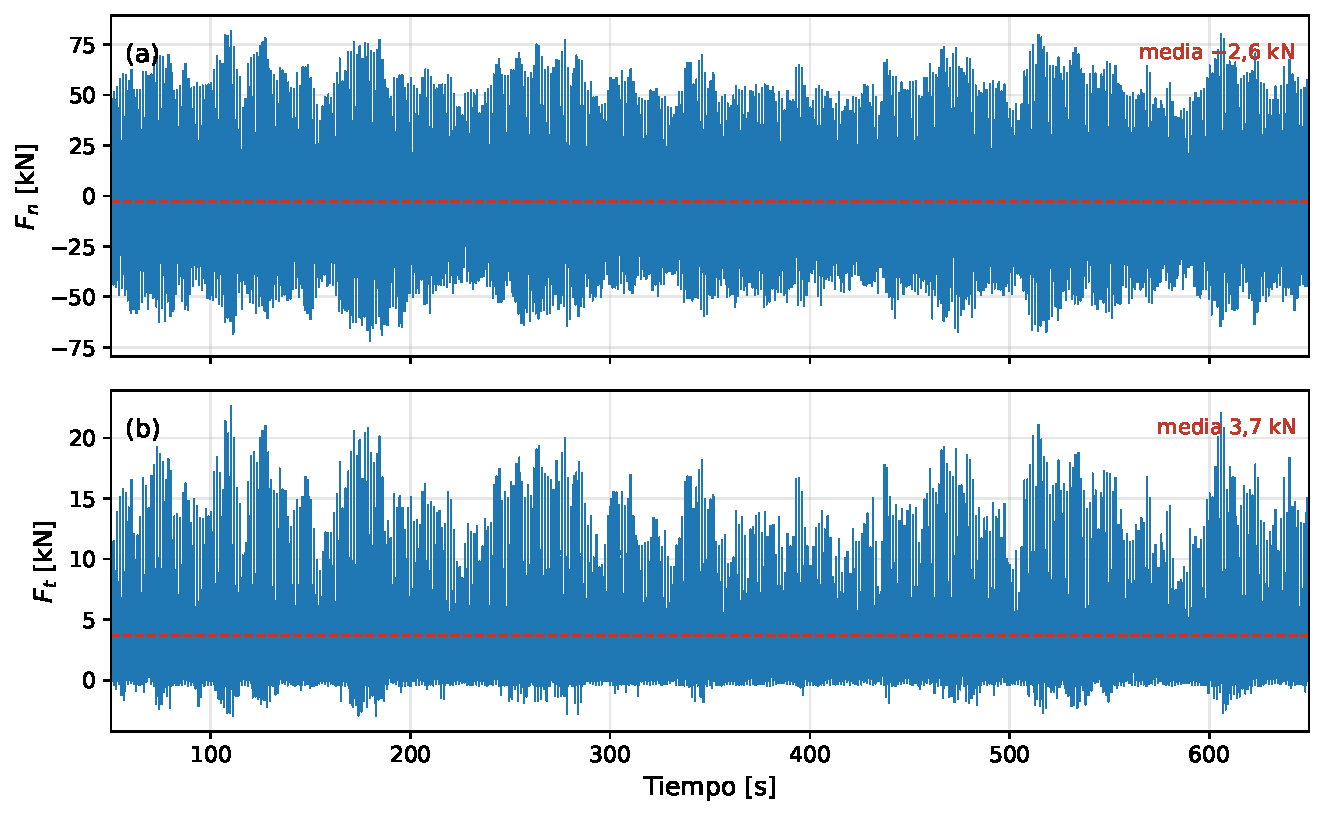
\includegraphics[width=0.85\textwidth]{Figuras/Figuras Anexo Fuerzas/fuerzas_xy_V18_S2.pdf}
    \caption{Fuerzas resultantes (a) $F_x$ y (b) $F_y$ en función del tiempo, $V = 18$~m/s, semilla $2$.}
    \label{fig:anexo_fuerzas_xy_V18_S2}
\end{figure}

\begin{figure}[H]
    \centering
    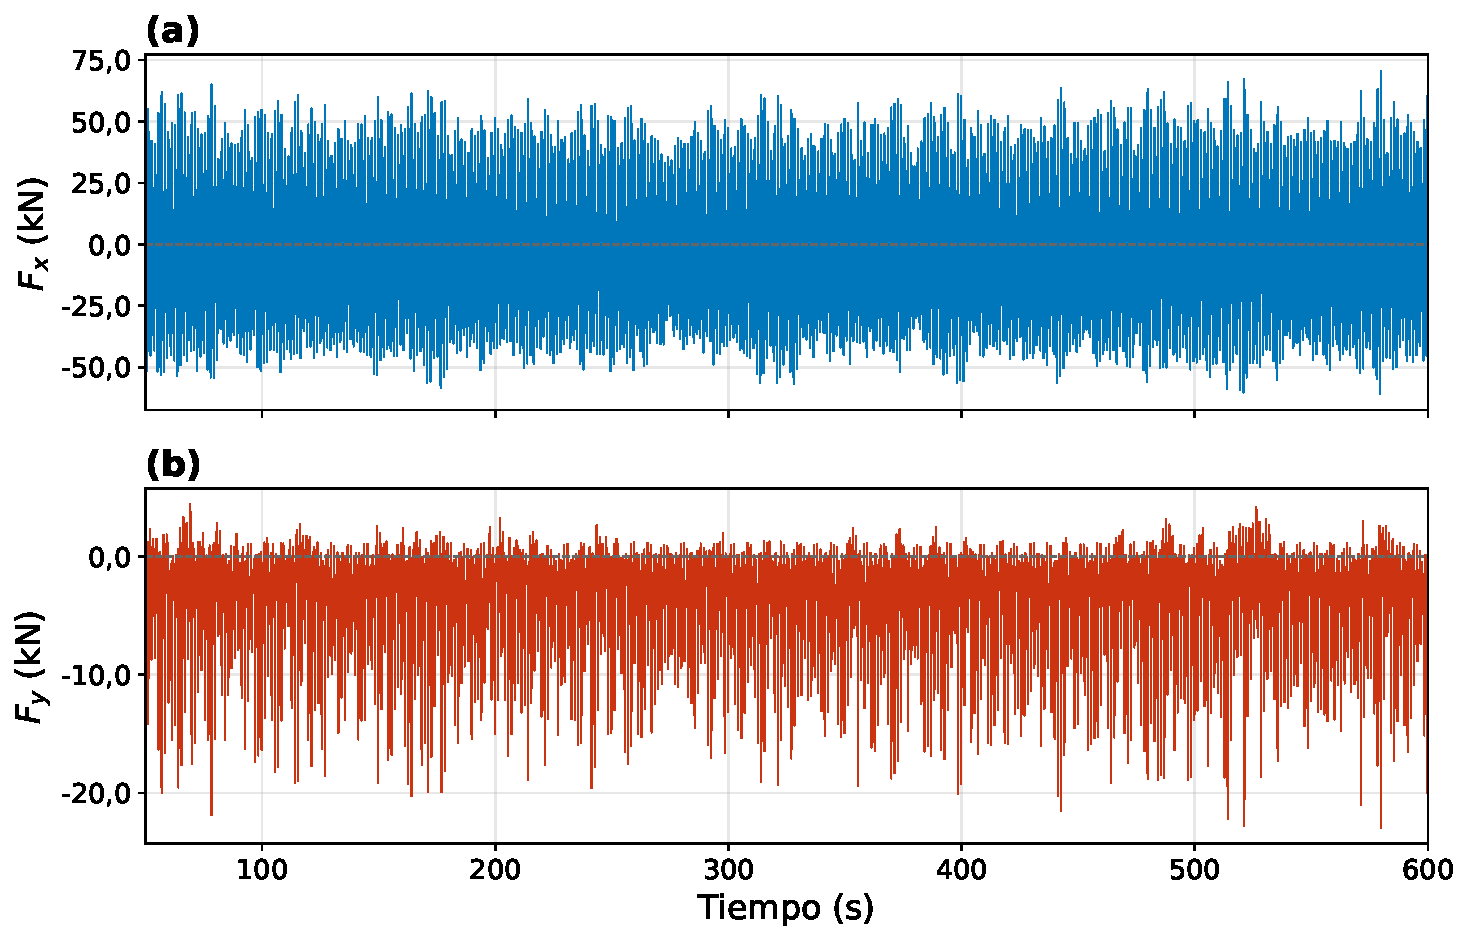
\includegraphics[width=0.85\textwidth]{Figuras/Figuras Anexo Fuerzas/fuerzas_xy_V18_S3.pdf}
    \caption{Fuerzas resultantes (a) $F_x$ y (b) $F_y$ en función del tiempo, $V = 18$~m/s, semilla $3$.}
    \label{fig:anexo_fuerzas_xy_V18_S3}
\end{figure}

\begin{figure}[H]
    \centering
    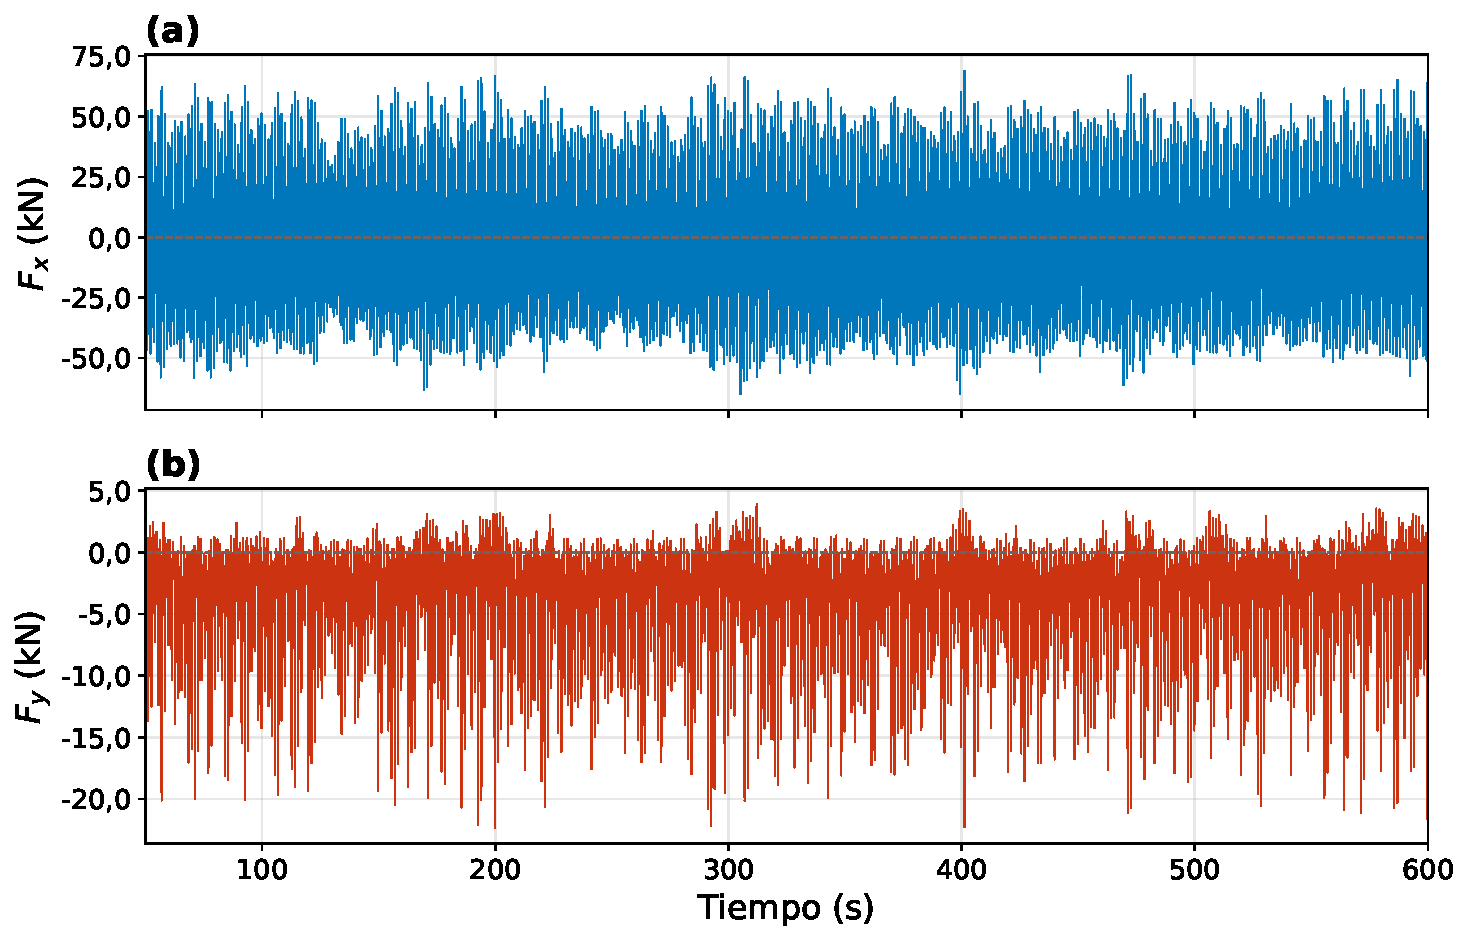
\includegraphics[width=0.85\textwidth]{Figuras/Figuras Anexo Fuerzas/fuerzas_xy_V18_S4.pdf}
    \caption{Fuerzas resultantes (a) $F_x$ y (b) $F_y$ en función del tiempo, $V = 18$~m/s, semilla $4$.}
    \label{fig:anexo_fuerzas_xy_V18_S4}
\end{figure}

\begin{figure}[H]
    \centering
    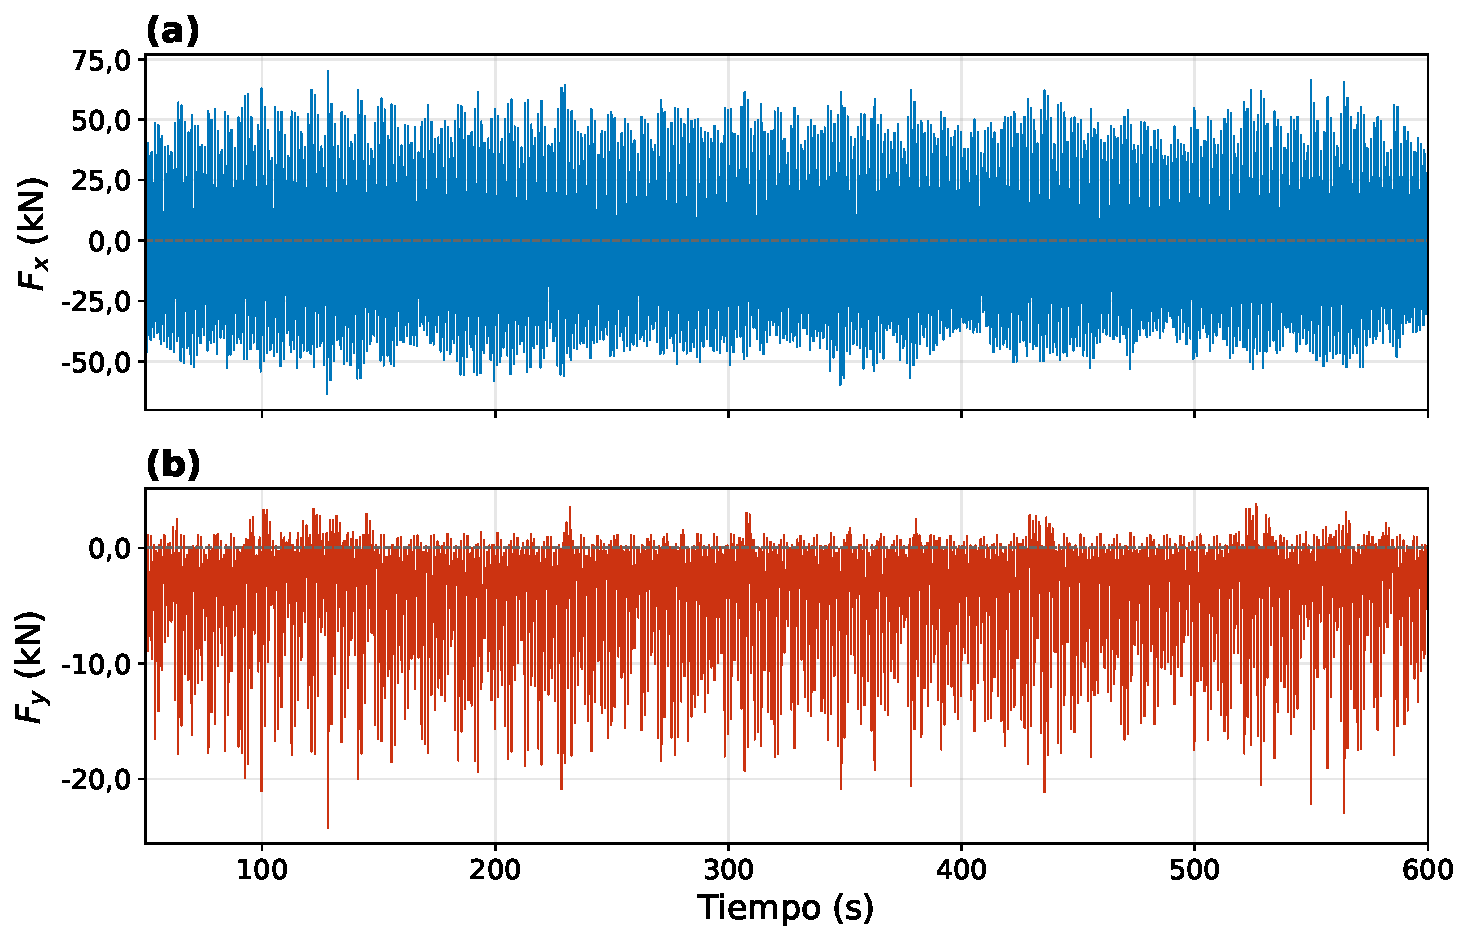
\includegraphics[width=0.85\textwidth]{Figuras/Figuras Anexo Fuerzas/fuerzas_xy_V18_S5.pdf}
    \caption{Fuerzas resultantes (a) $F_x$ y (b) $F_y$ en función del tiempo, $V = 18$~m/s, semilla $5$.}
    \label{fig:anexo_fuerzas_xy_V18_S5}
\end{figure}

\begin{figure}[H]
    \centering
    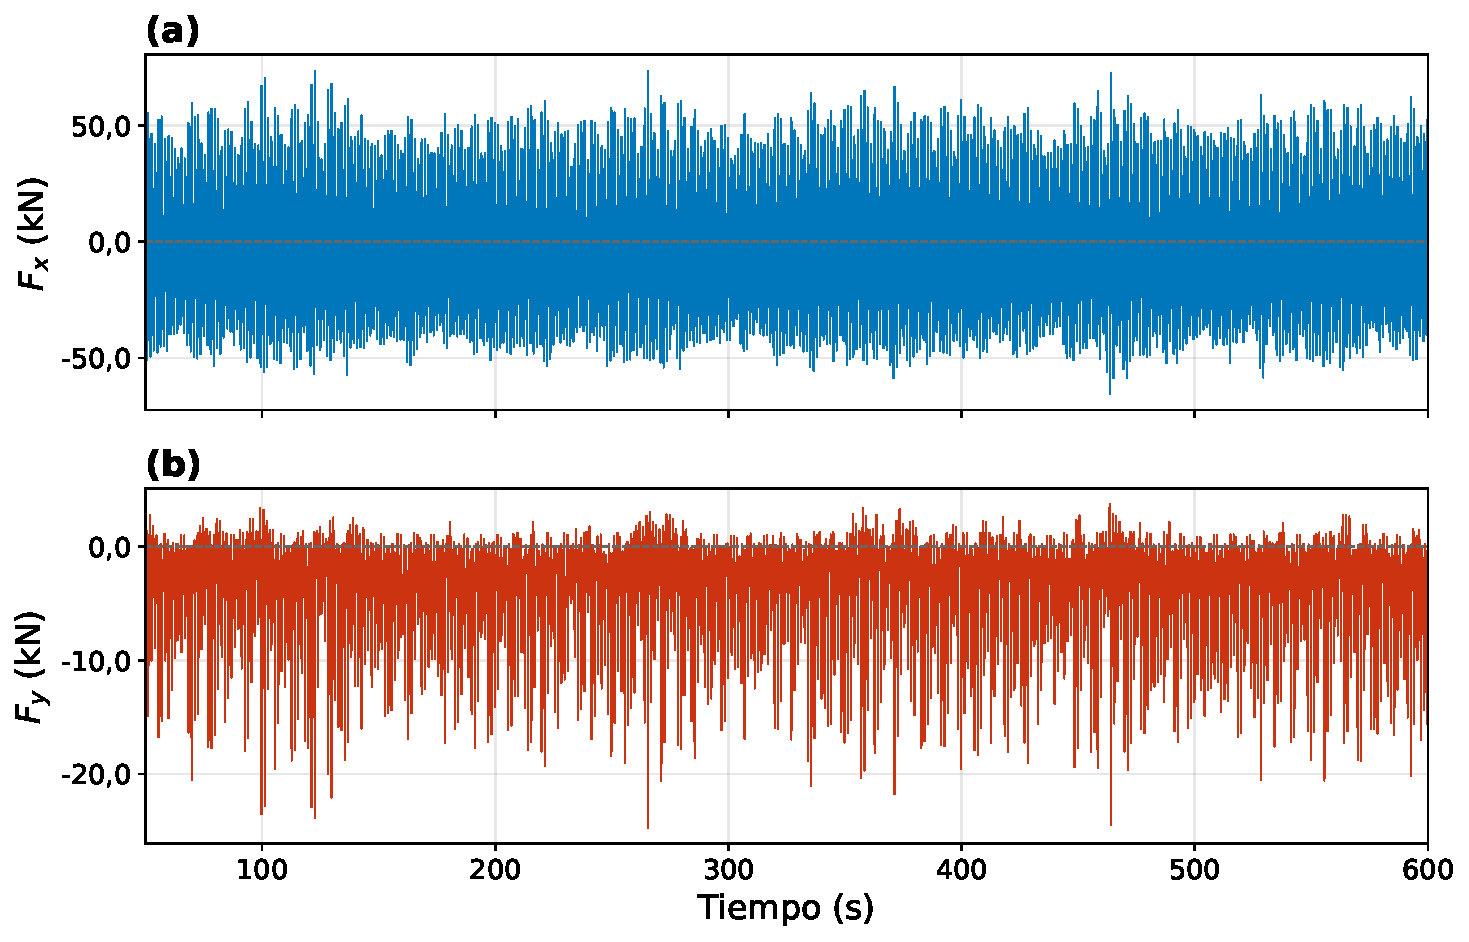
\includegraphics[width=0.85\textwidth]{Figuras/Figuras Anexo Fuerzas/fuerzas_xy_V18_S6.pdf}
    \caption{Fuerzas resultantes (a) $F_x$ y (b) $F_y$ en función del tiempo, $V = 18$~m/s, semilla $6$.}
    \label{fig:anexo_fuerzas_xy_V18_S6}
\end{figure}

\begin{figure}[H]
    \centering
    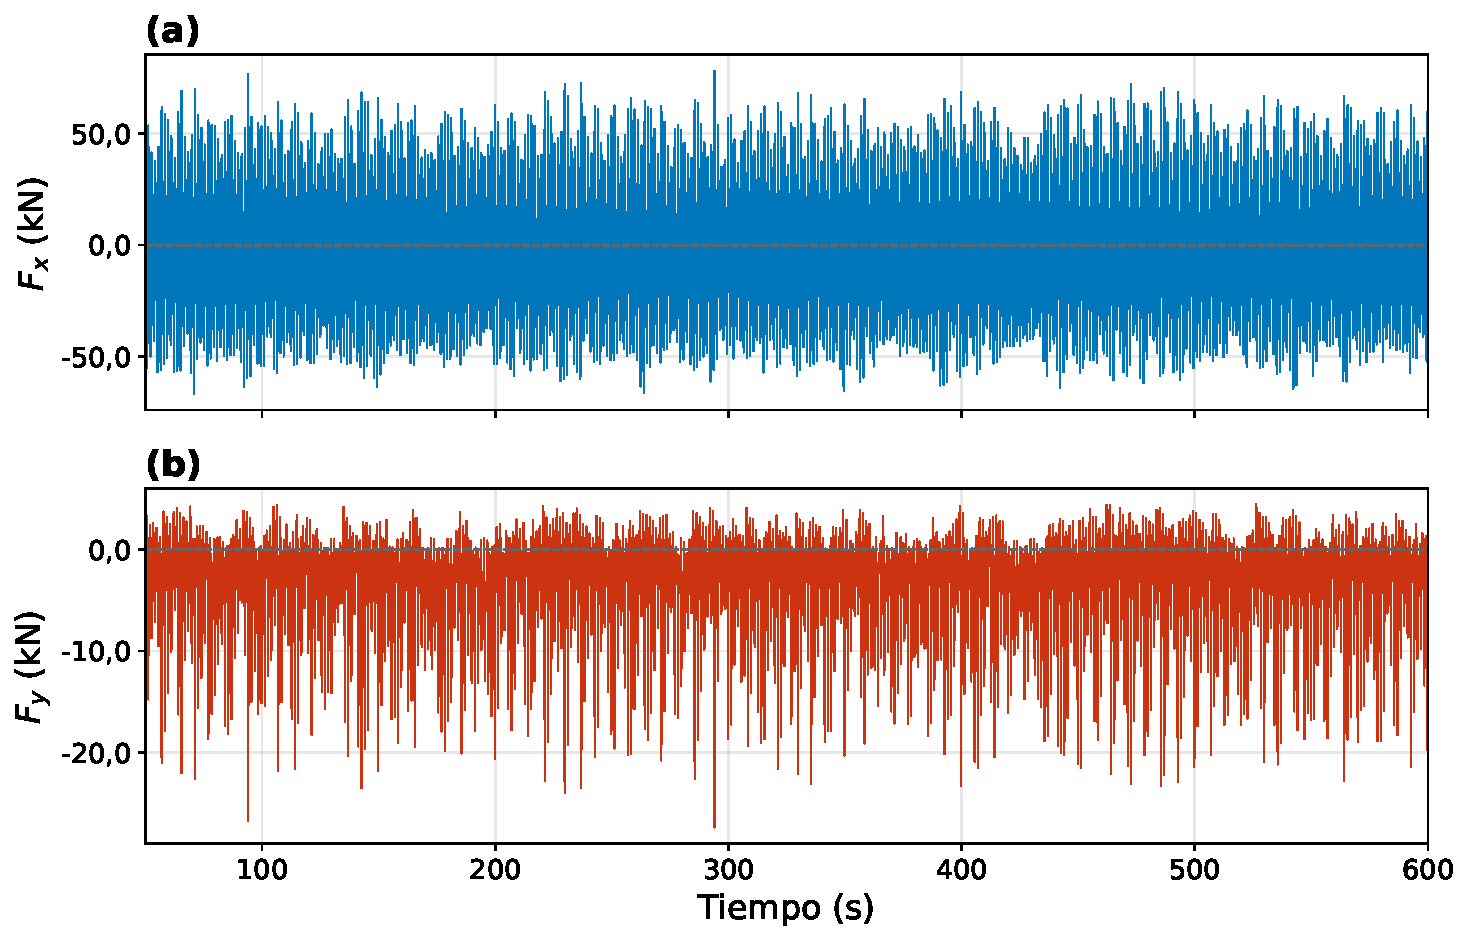
\includegraphics[width=0.85\textwidth]{Figuras/Figuras Anexo Fuerzas/fuerzas_xy_V20_S1.pdf}
    \caption{Fuerzas resultantes (a) $F_x$ y (b) $F_y$ en función del tiempo, $V = 20$~m/s, semilla $1$.}
    \label{fig:anexo_fuerzas_xy_V20_S1}
\end{figure}

\begin{figure}[H]
    \centering
    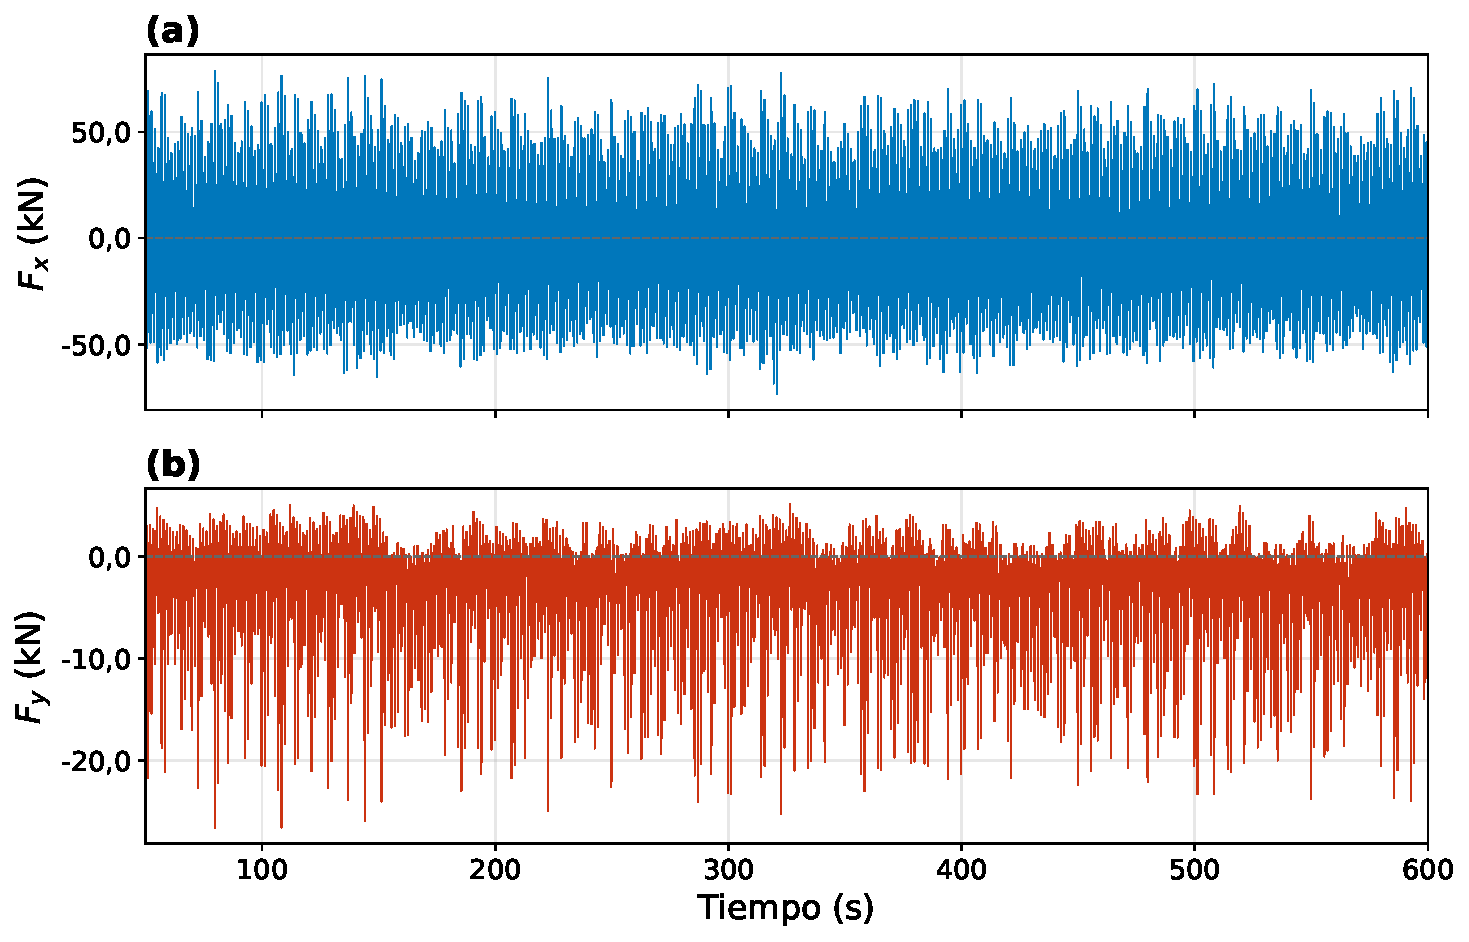
\includegraphics[width=0.85\textwidth]{Figuras/Figuras Anexo Fuerzas/fuerzas_xy_V20_S2.pdf}
    \caption{Fuerzas resultantes (a) $F_x$ y (b) $F_y$ en función del tiempo, $V = 20$~m/s, semilla $2$.}
    \label{fig:anexo_fuerzas_xy_V20_S2}
\end{figure}

\begin{figure}[H]
    \centering
    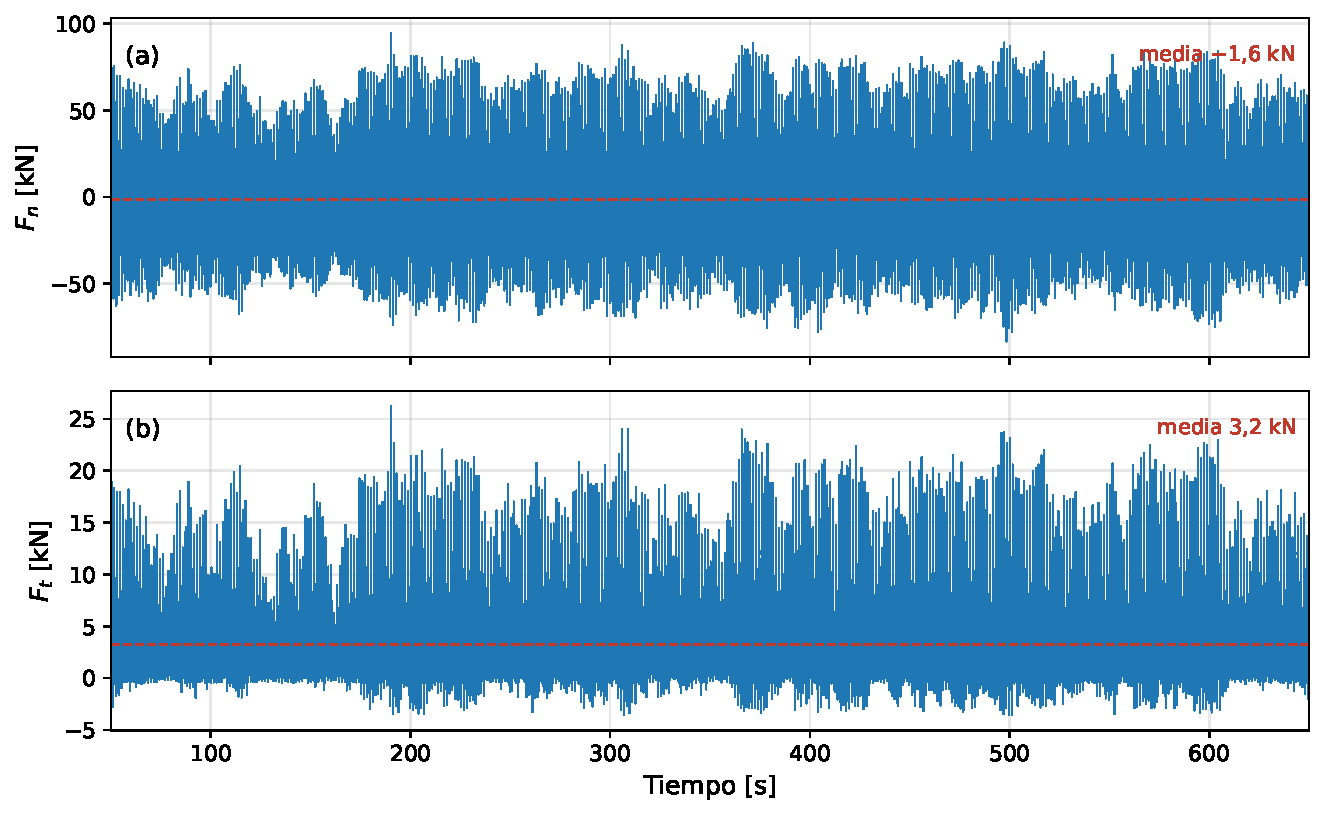
\includegraphics[width=0.85\textwidth]{Figuras/Figuras Anexo Fuerzas/fuerzas_xy_V20_S3.pdf}
    \caption{Fuerzas resultantes (a) $F_x$ y (b) $F_y$ en función del tiempo, $V = 20$~m/s, semilla $3$.}
    \label{fig:anexo_fuerzas_xy_V20_S3}
\end{figure}

\begin{figure}[H]
    \centering
    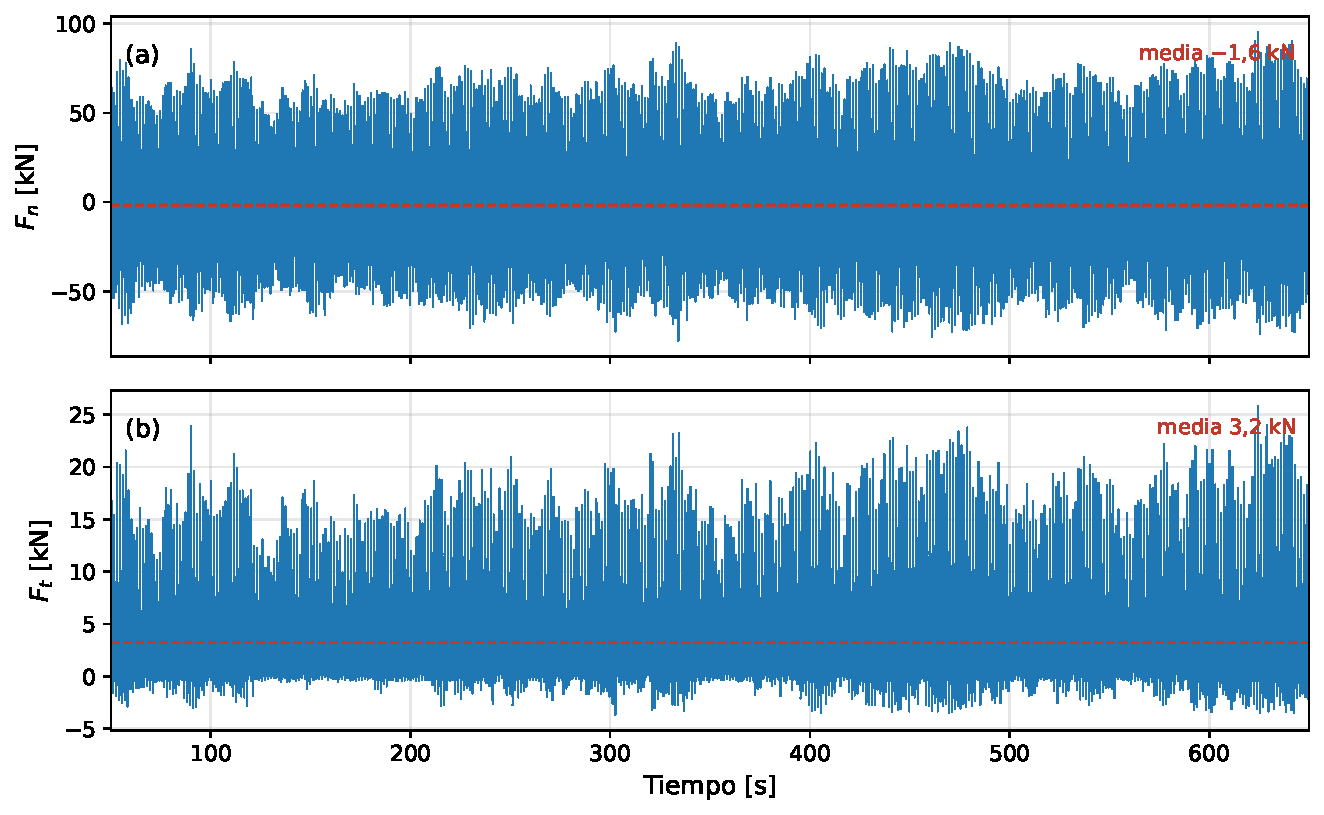
\includegraphics[width=0.85\textwidth]{Figuras/Figuras Anexo Fuerzas/fuerzas_xy_V20_S4.pdf}
    \caption{Fuerzas resultantes (a) $F_x$ y (b) $F_y$ en función del tiempo, $V = 20$~m/s, semilla $4$.}
    \label{fig:anexo_fuerzas_xy_V20_S4}
\end{figure}

\begin{figure}[H]
    \centering
    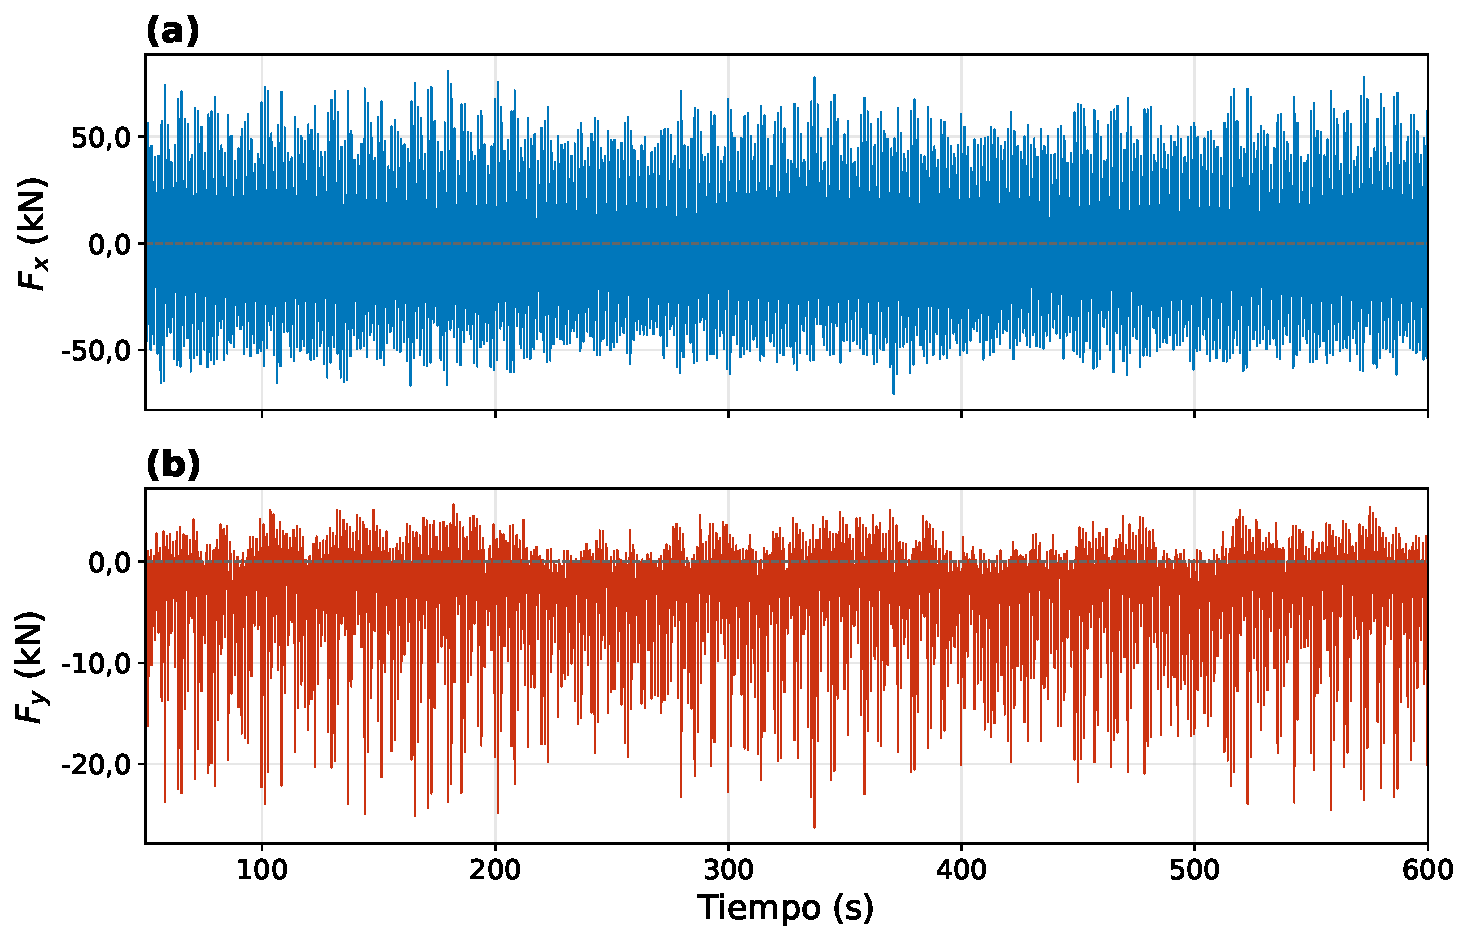
\includegraphics[width=0.85\textwidth]{Figuras/Figuras Anexo Fuerzas/fuerzas_xy_V20_S5.pdf}
    \caption{Fuerzas resultantes (a) $F_x$ y (b) $F_y$ en función del tiempo, $V = 20$~m/s, semilla $5$.}
    \label{fig:anexo_fuerzas_xy_V20_S5}
\end{figure}

\begin{figure}[H]
    \centering
    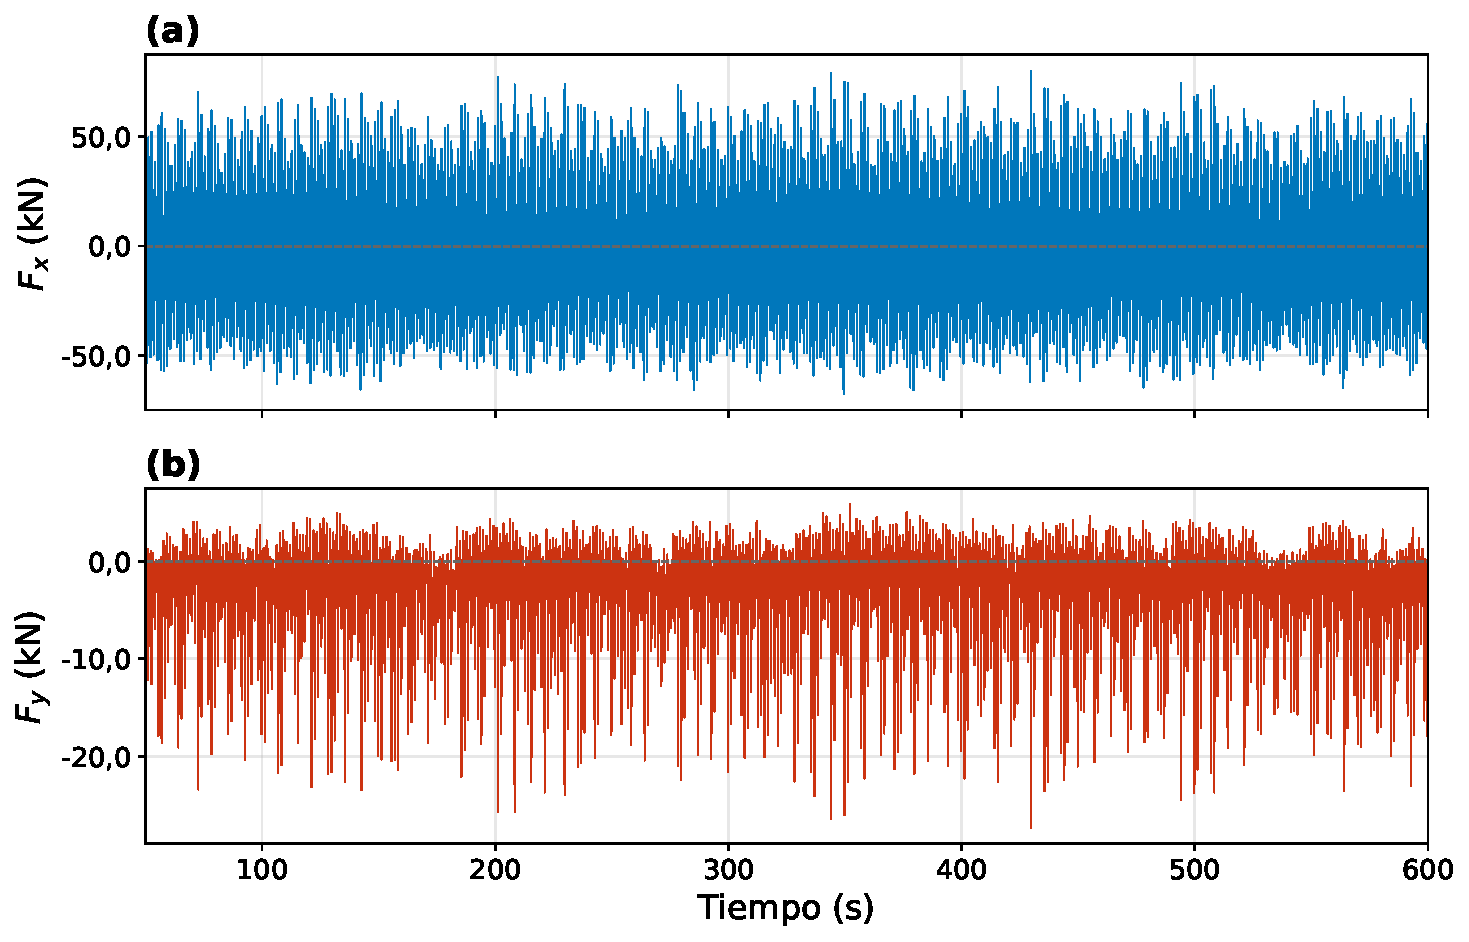
\includegraphics[width=0.85\textwidth]{Figuras/Figuras Anexo Fuerzas/fuerzas_xy_V20_S6.pdf}
    \caption{Fuerzas resultantes (a) $F_x$ y (b) $F_y$ en función del tiempo, $V = 20$~m/s, semilla $6$.}
    \label{fig:anexo_fuerzas_xy_V20_S6}
\end{figure}

\begin{figure}[H]
    \centering
    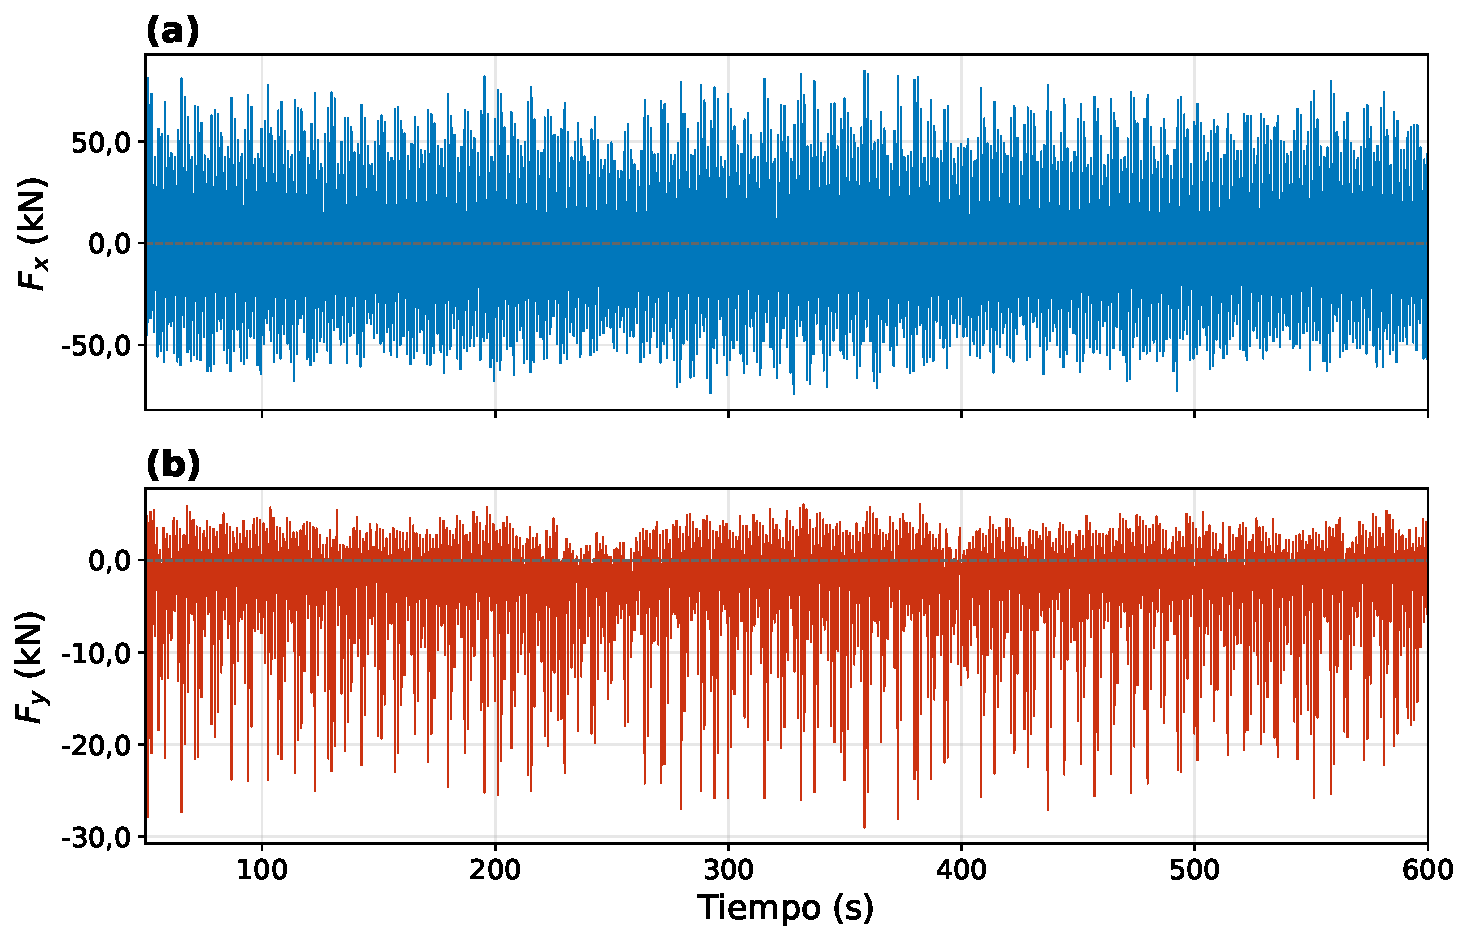
\includegraphics[width=0.85\textwidth]{Figuras/Figuras Anexo Fuerzas/fuerzas_xy_V22_S1.pdf}
    \caption{Fuerzas resultantes (a) $F_x$ y (b) $F_y$ en función del tiempo, $V = 22$~m/s, semilla $1$.}
    \label{fig:anexo_fuerzas_xy_V22_S1}
\end{figure}

\begin{figure}[H]
    \centering
    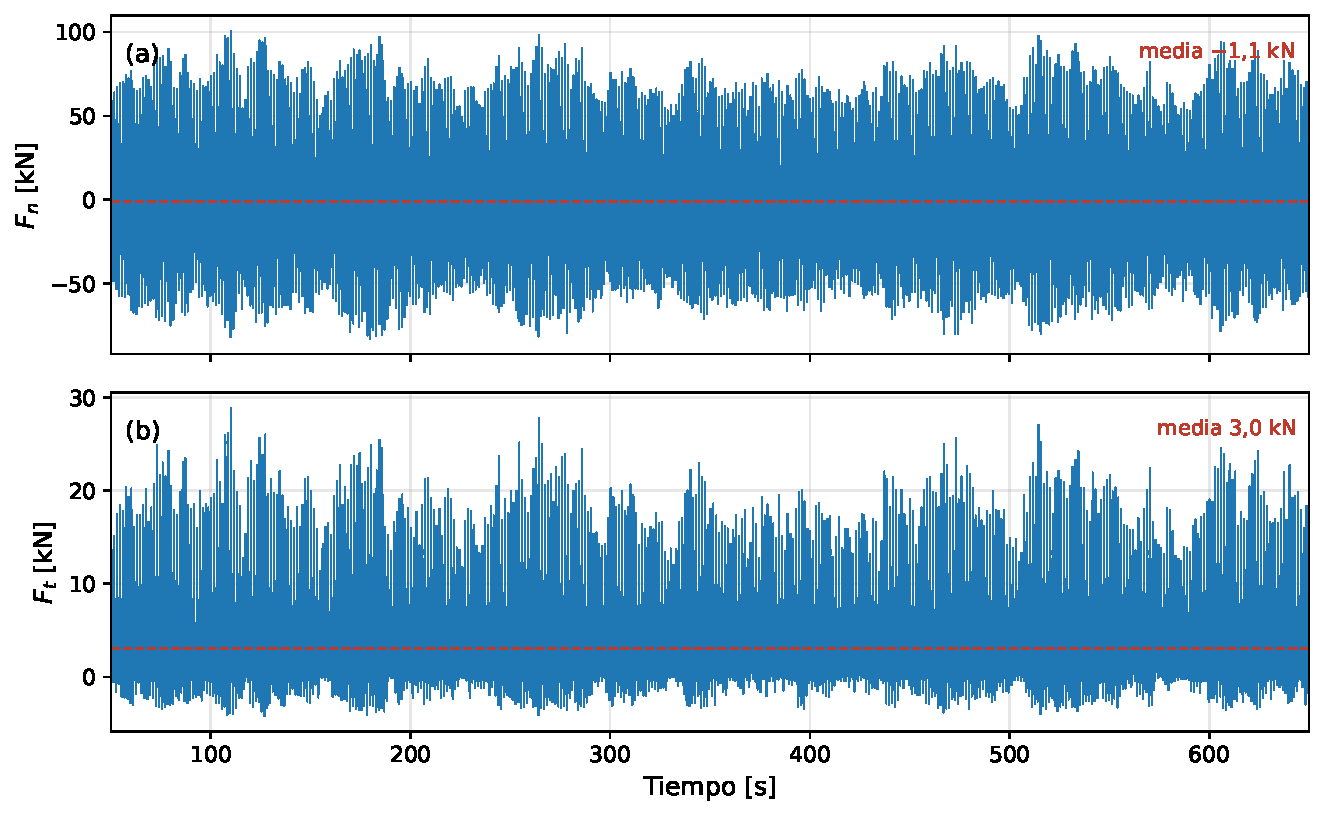
\includegraphics[width=0.85\textwidth]{Figuras/Figuras Anexo Fuerzas/fuerzas_xy_V22_S2.pdf}
    \caption{Fuerzas resultantes (a) $F_x$ y (b) $F_y$ en función del tiempo, $V = 22$~m/s, semilla $2$.}
    \label{fig:anexo_fuerzas_xy_V22_S2}
\end{figure}

\begin{figure}[H]
    \centering
    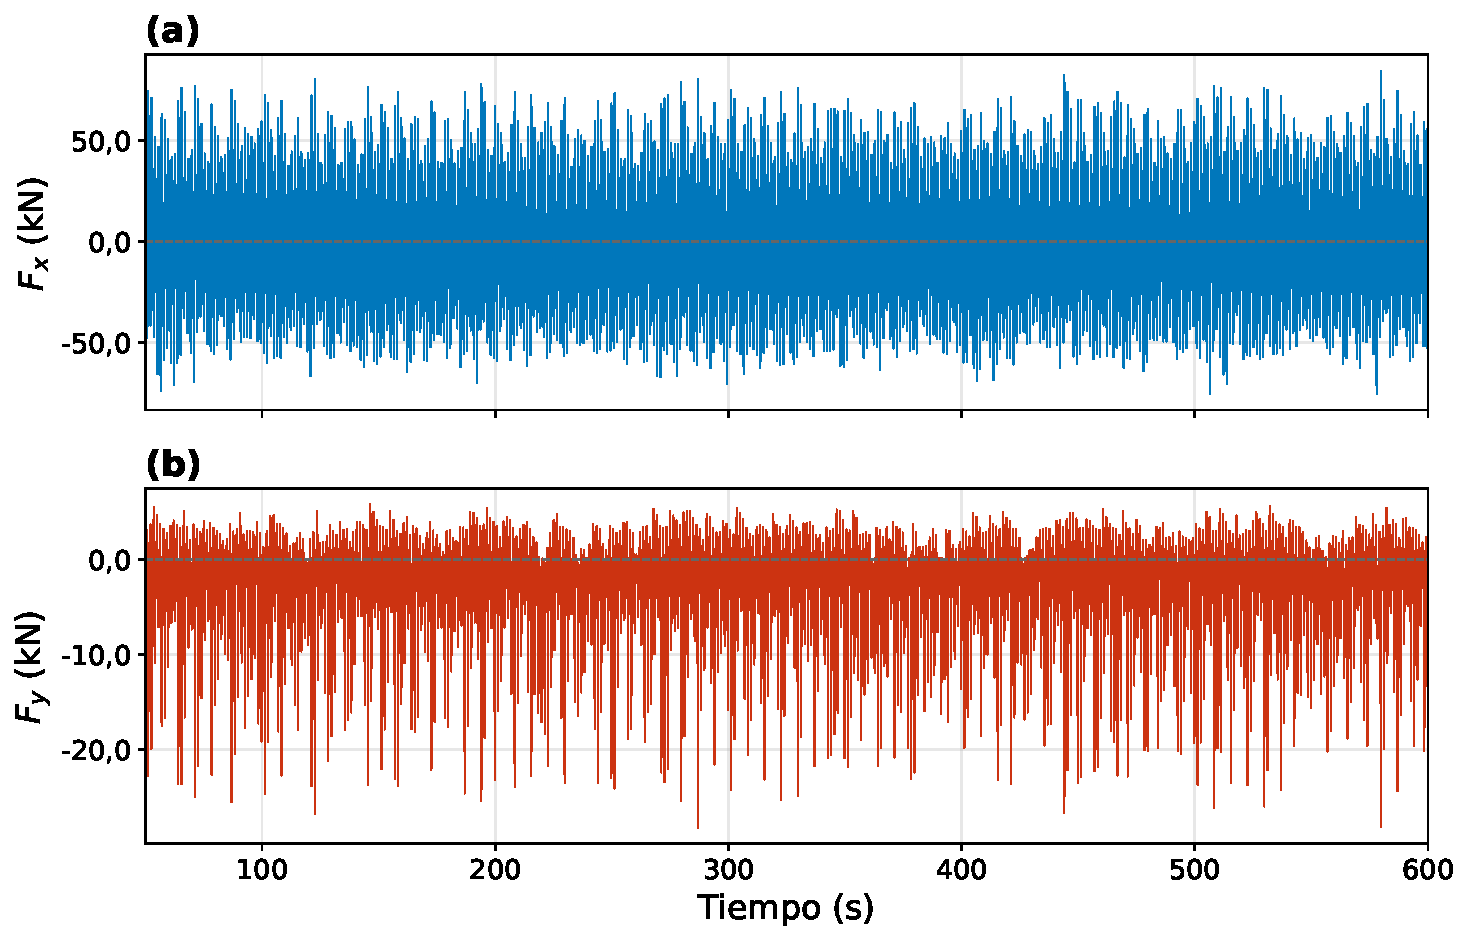
\includegraphics[width=0.85\textwidth]{Figuras/Figuras Anexo Fuerzas/fuerzas_xy_V22_S3.pdf}
    \caption{Fuerzas resultantes (a) $F_x$ y (b) $F_y$ en función del tiempo, $V = 22$~m/s, semilla $3$.}
    \label{fig:anexo_fuerzas_xy_V22_S3}
\end{figure}

\begin{figure}[H]
    \centering
    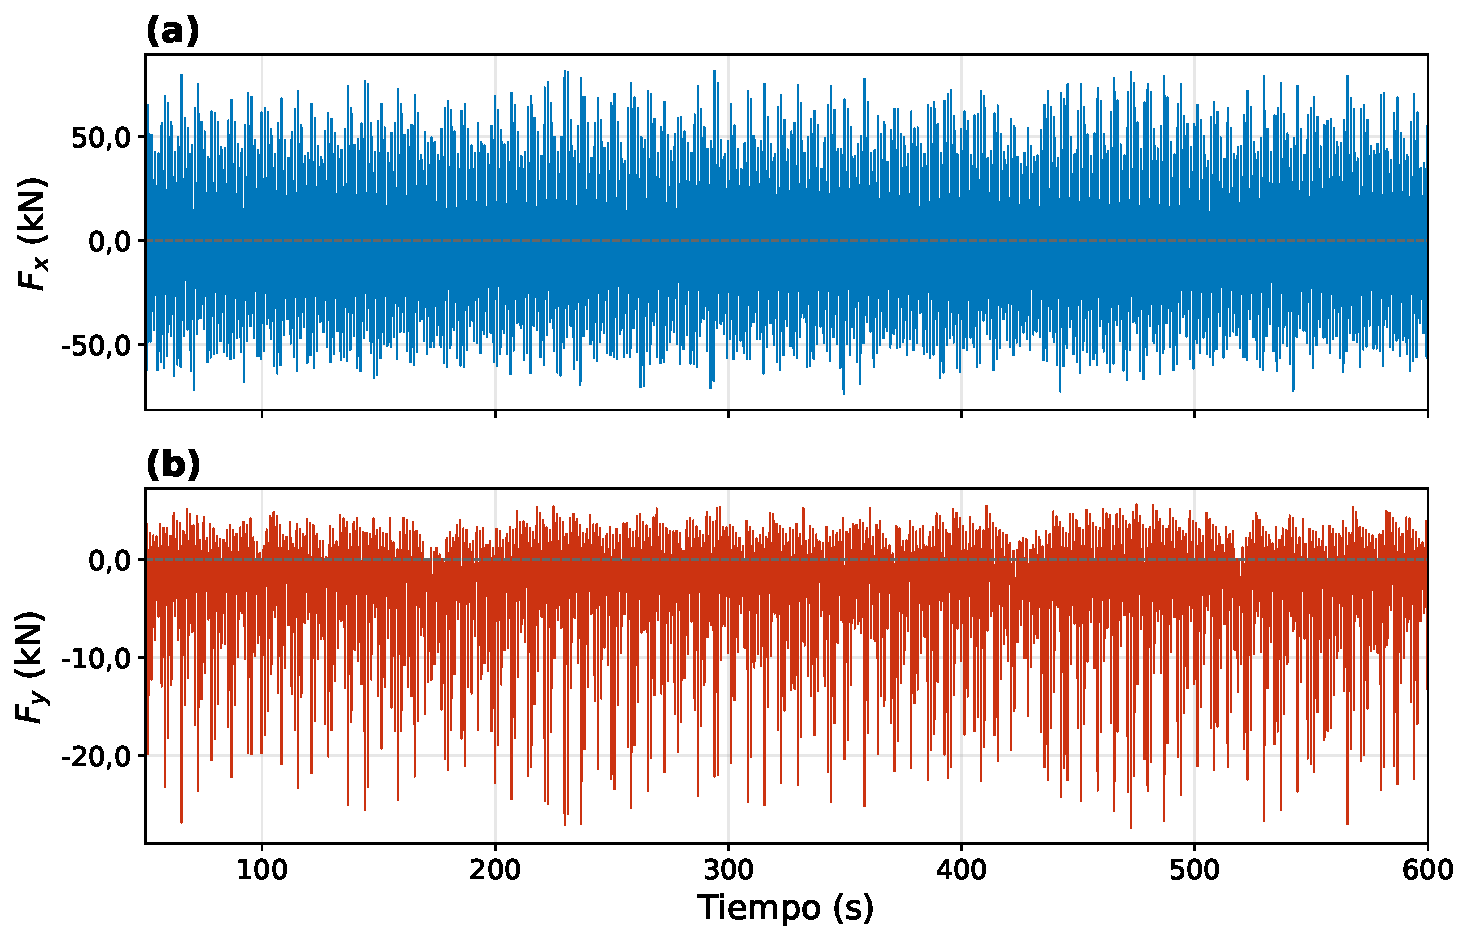
\includegraphics[width=0.85\textwidth]{Figuras/Figuras Anexo Fuerzas/fuerzas_xy_V22_S4.pdf}
    \caption{Fuerzas resultantes (a) $F_x$ y (b) $F_y$ en función del tiempo, $V = 22$~m/s, semilla $4$.}
    \label{fig:anexo_fuerzas_xy_V22_S4}
\end{figure}

\begin{figure}[H]
    \centering
    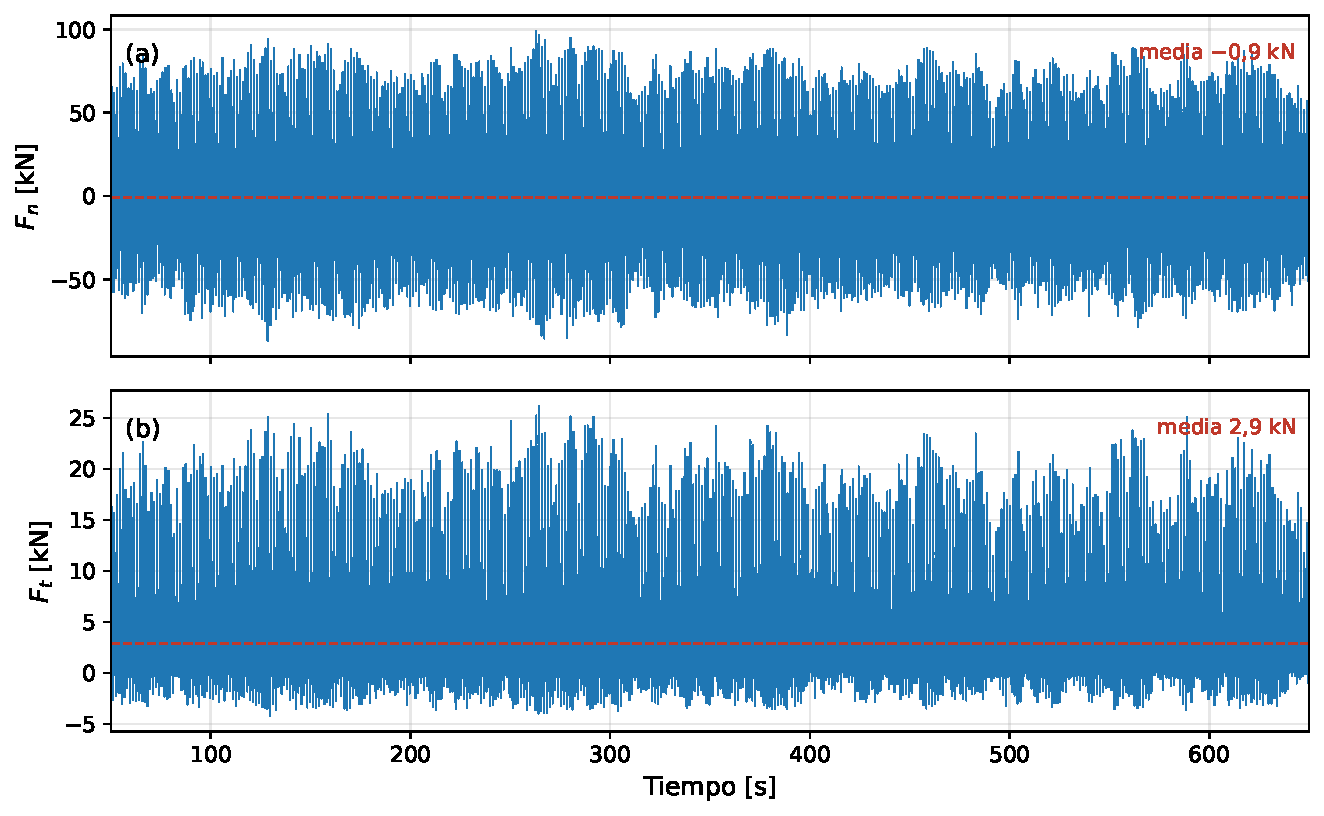
\includegraphics[width=0.85\textwidth]{Figuras/Figuras Anexo Fuerzas/fuerzas_xy_V22_S5.pdf}
    \caption{Fuerzas resultantes (a) $F_x$ y (b) $F_y$ en función del tiempo, $V = 22$~m/s, semilla $5$.}
    \label{fig:anexo_fuerzas_xy_V22_S5}
\end{figure}

\begin{figure}[H]
    \centering
    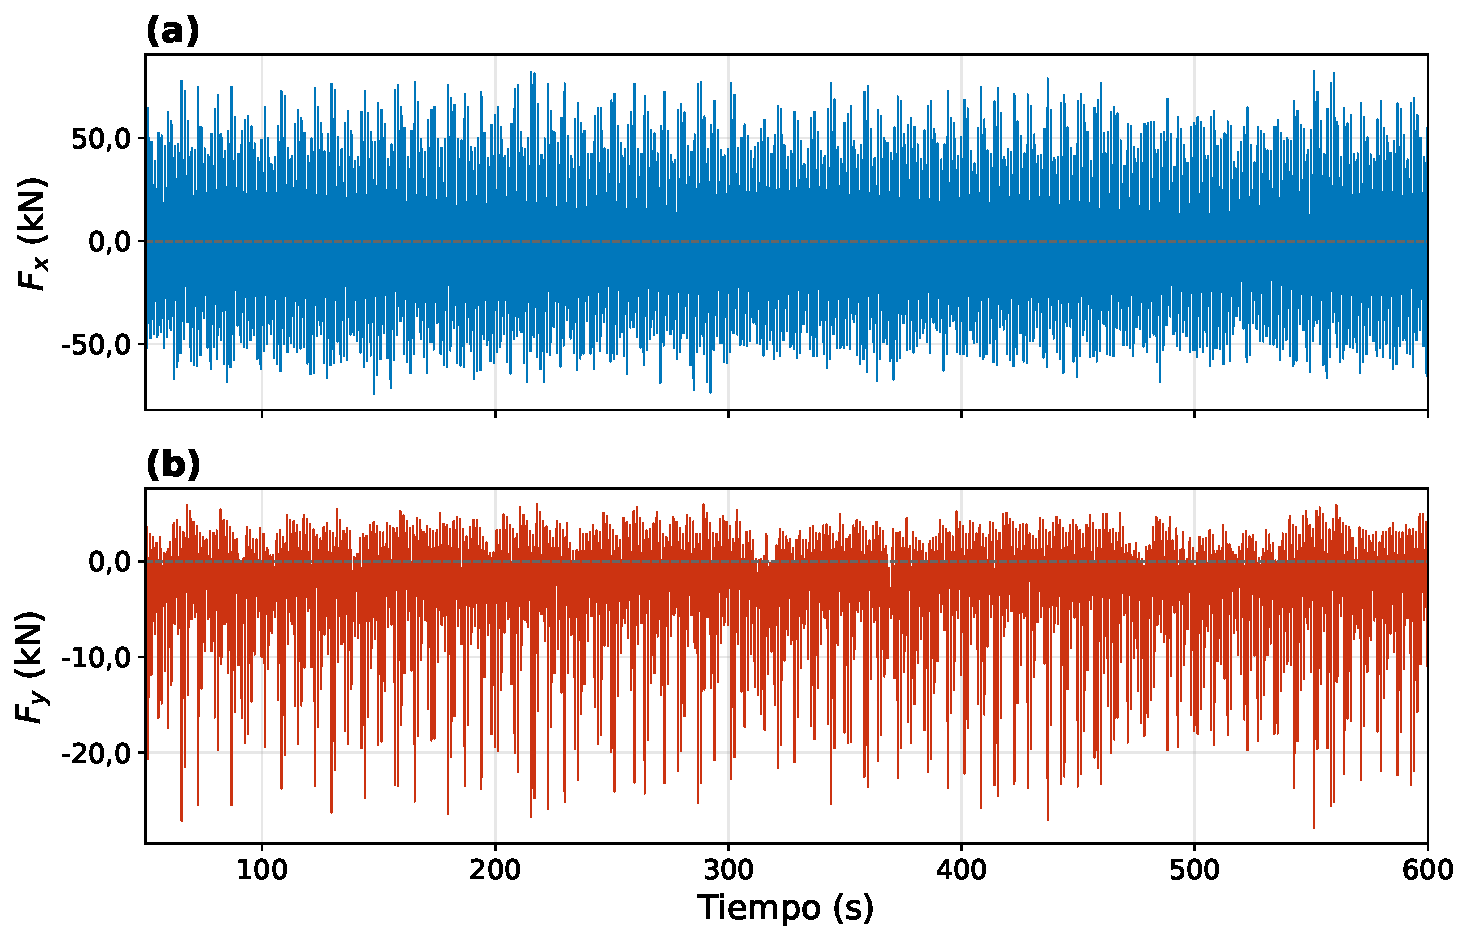
\includegraphics[width=0.85\textwidth]{Figuras/Figuras Anexo Fuerzas/fuerzas_xy_V22_S6.pdf}
    \caption{Fuerzas resultantes (a) $F_x$ y (b) $F_y$ en función del tiempo, $V = 22$~m/s, semilla $6$.}
    \label{fig:anexo_fuerzas_xy_V22_S6}
\end{figure}

\begin{figure}[H]
    \centering
    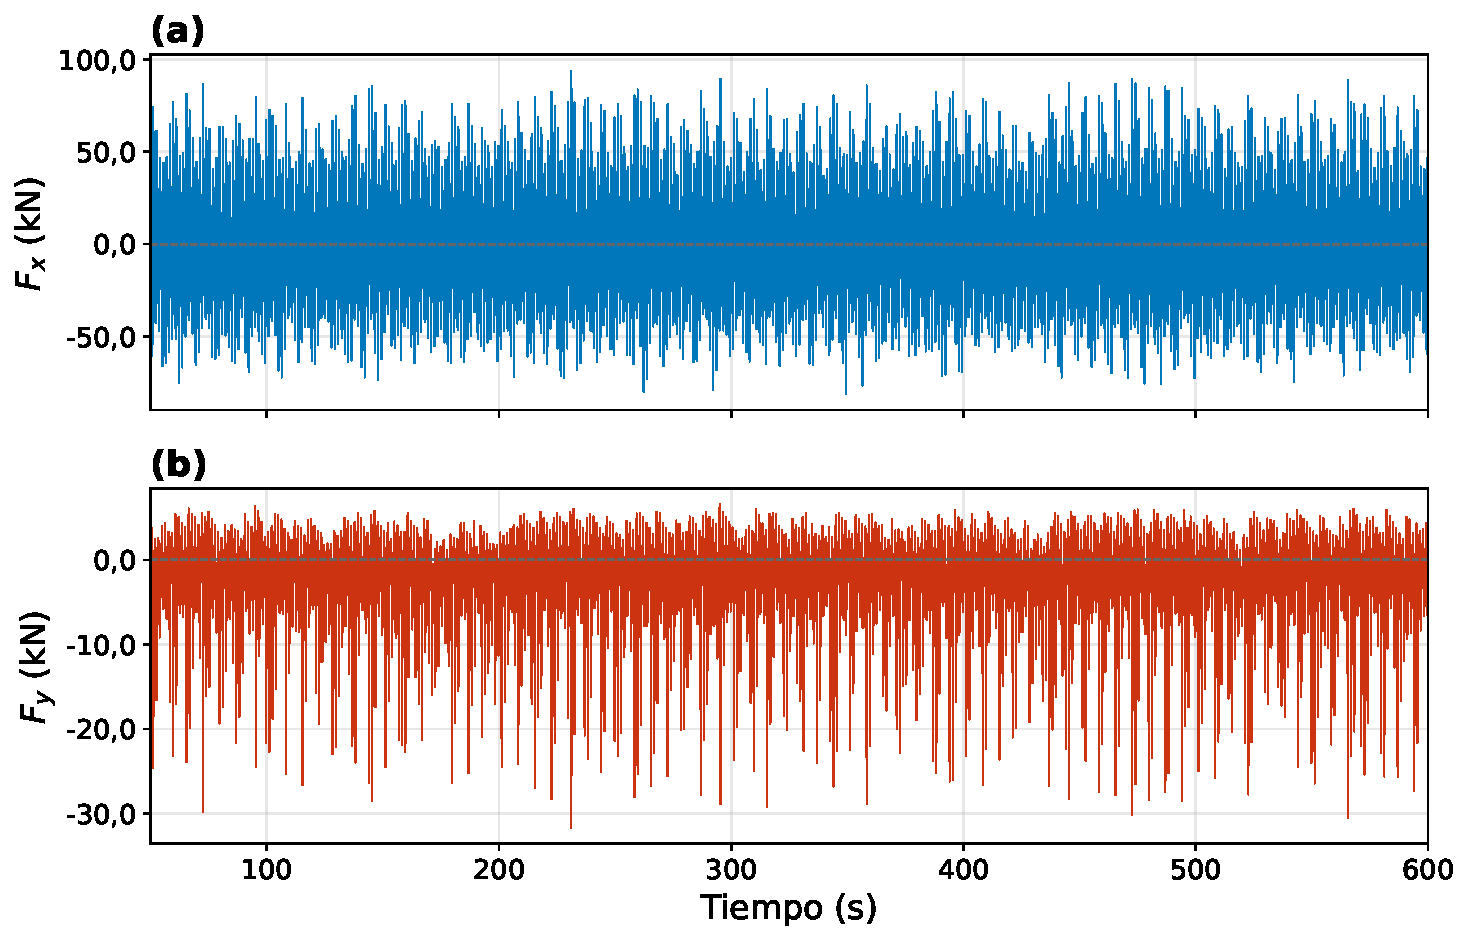
\includegraphics[width=0.85\textwidth]{Figuras/Figuras Anexo Fuerzas/fuerzas_xy_V24_S1.pdf}
    \caption{Fuerzas resultantes (a) $F_x$ y (b) $F_y$ en función del tiempo, $V = 24$~m/s, semilla $1$.}
    \label{fig:anexo_fuerzas_xy_V24_S1}
\end{figure}

\begin{figure}[H]
    \centering
    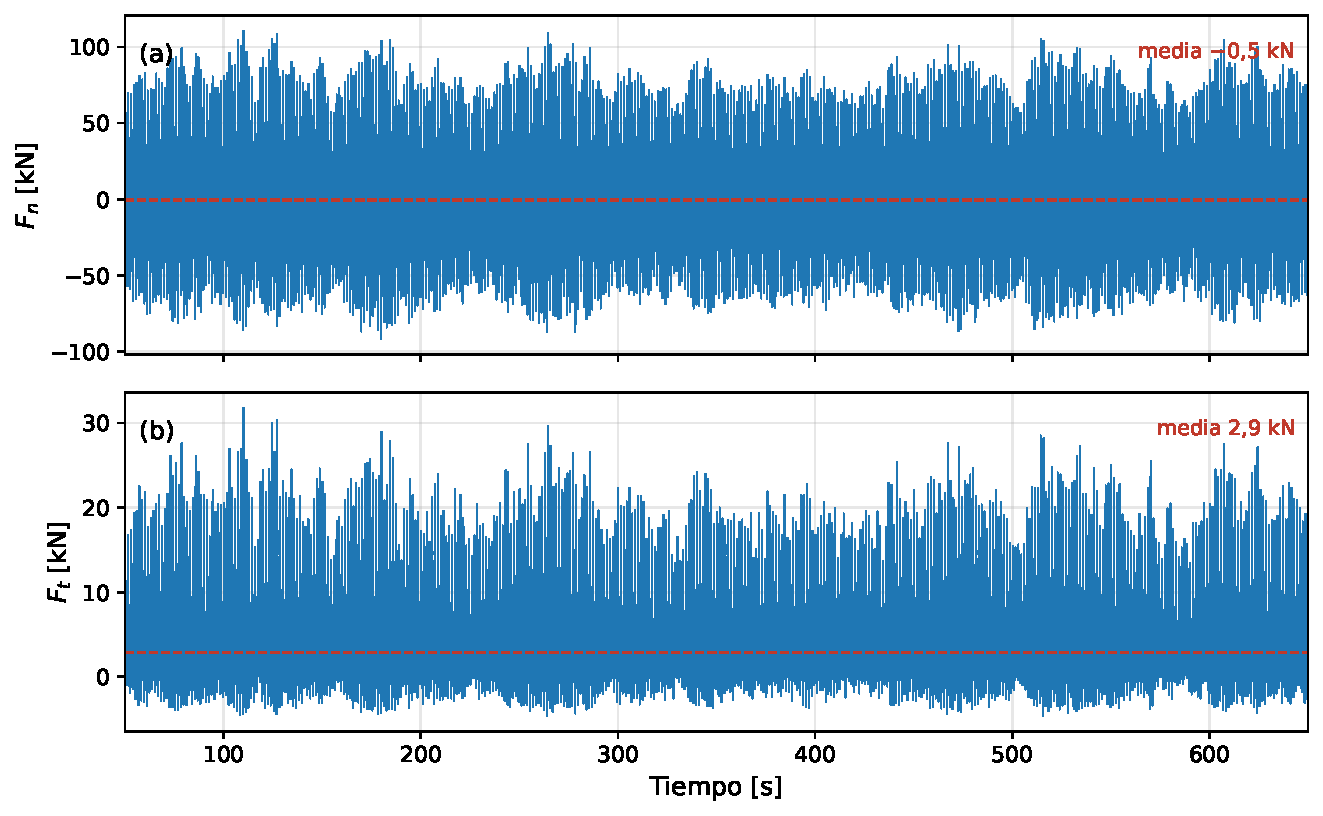
\includegraphics[width=0.85\textwidth]{Figuras/Figuras Anexo Fuerzas/fuerzas_xy_V24_S2.pdf}
    \caption{Fuerzas resultantes (a) $F_x$ y (b) $F_y$ en función del tiempo, $V = 24$~m/s, semilla $2$.}
    \label{fig:anexo_fuerzas_xy_V24_S2}
\end{figure}

\begin{figure}[H]
    \centering
    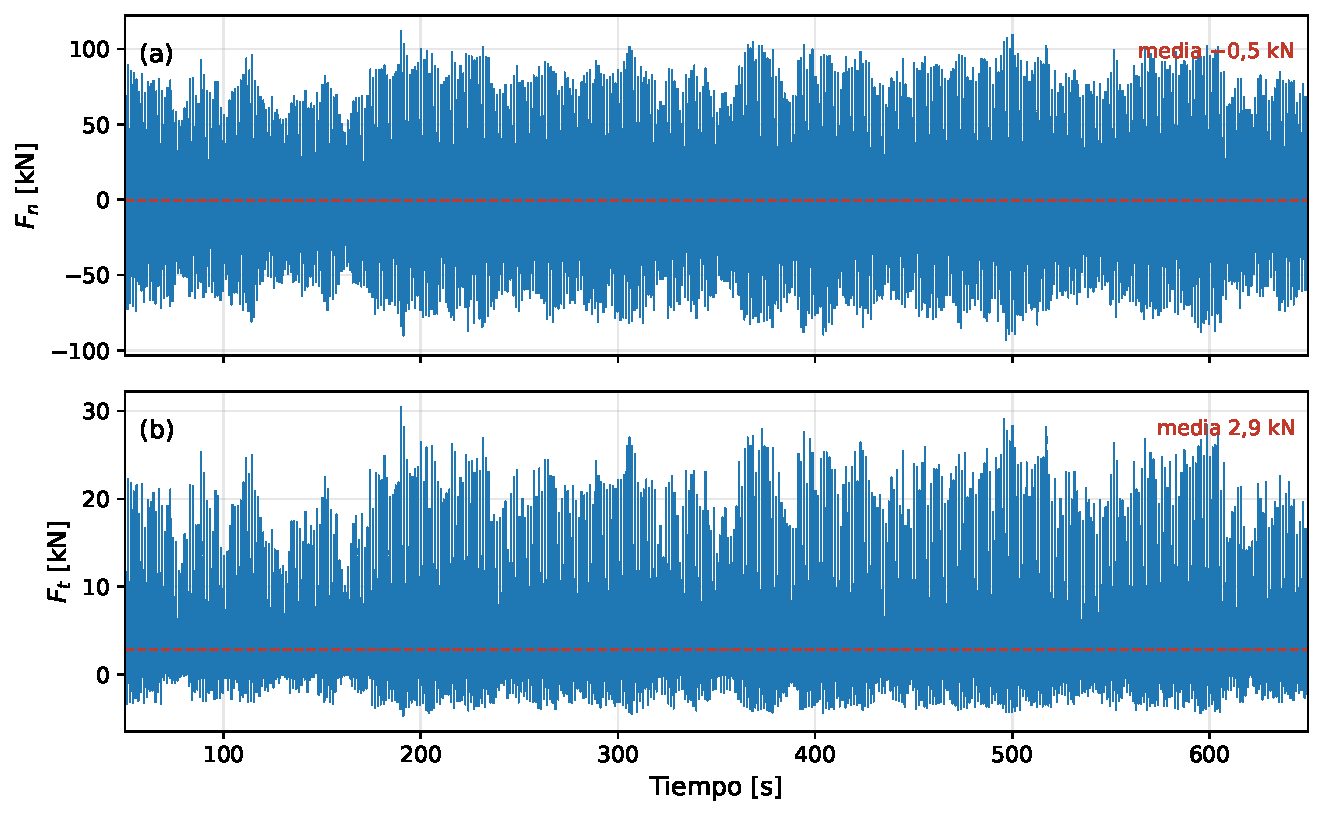
\includegraphics[width=0.85\textwidth]{Figuras/Figuras Anexo Fuerzas/fuerzas_xy_V24_S3.pdf}
    \caption{Fuerzas resultantes (a) $F_x$ y (b) $F_y$ en función del tiempo, $V = 24$~m/s, semilla $3$.}
    \label{fig:anexo_fuerzas_xy_V24_S3}
\end{figure}

\begin{figure}[H]
    \centering
    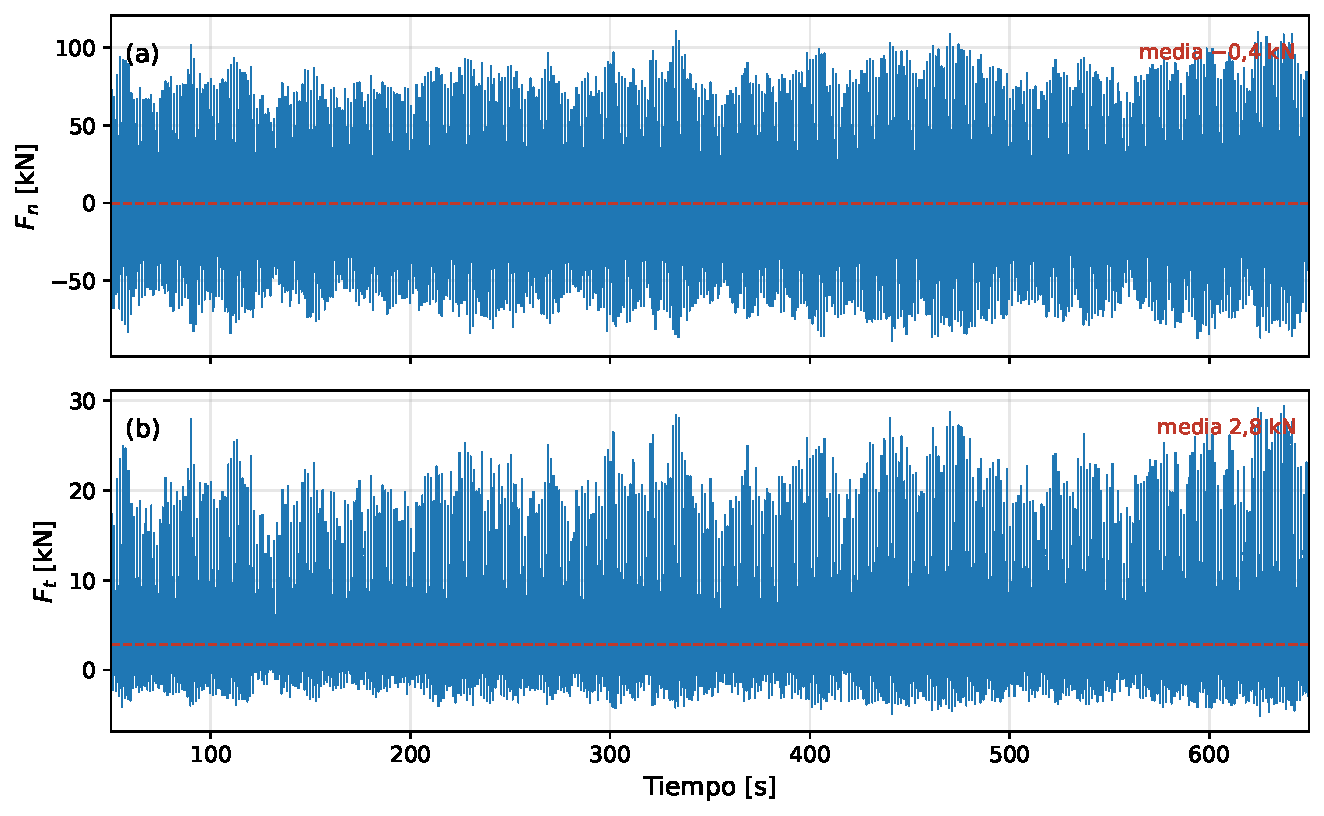
\includegraphics[width=0.85\textwidth]{Figuras/Figuras Anexo Fuerzas/fuerzas_xy_V24_S4.pdf}
    \caption{Fuerzas resultantes (a) $F_x$ y (b) $F_y$ en función del tiempo, $V = 24$~m/s, semilla $4$.}
    \label{fig:anexo_fuerzas_xy_V24_S4}
\end{figure}

\begin{figure}[H]
    \centering
    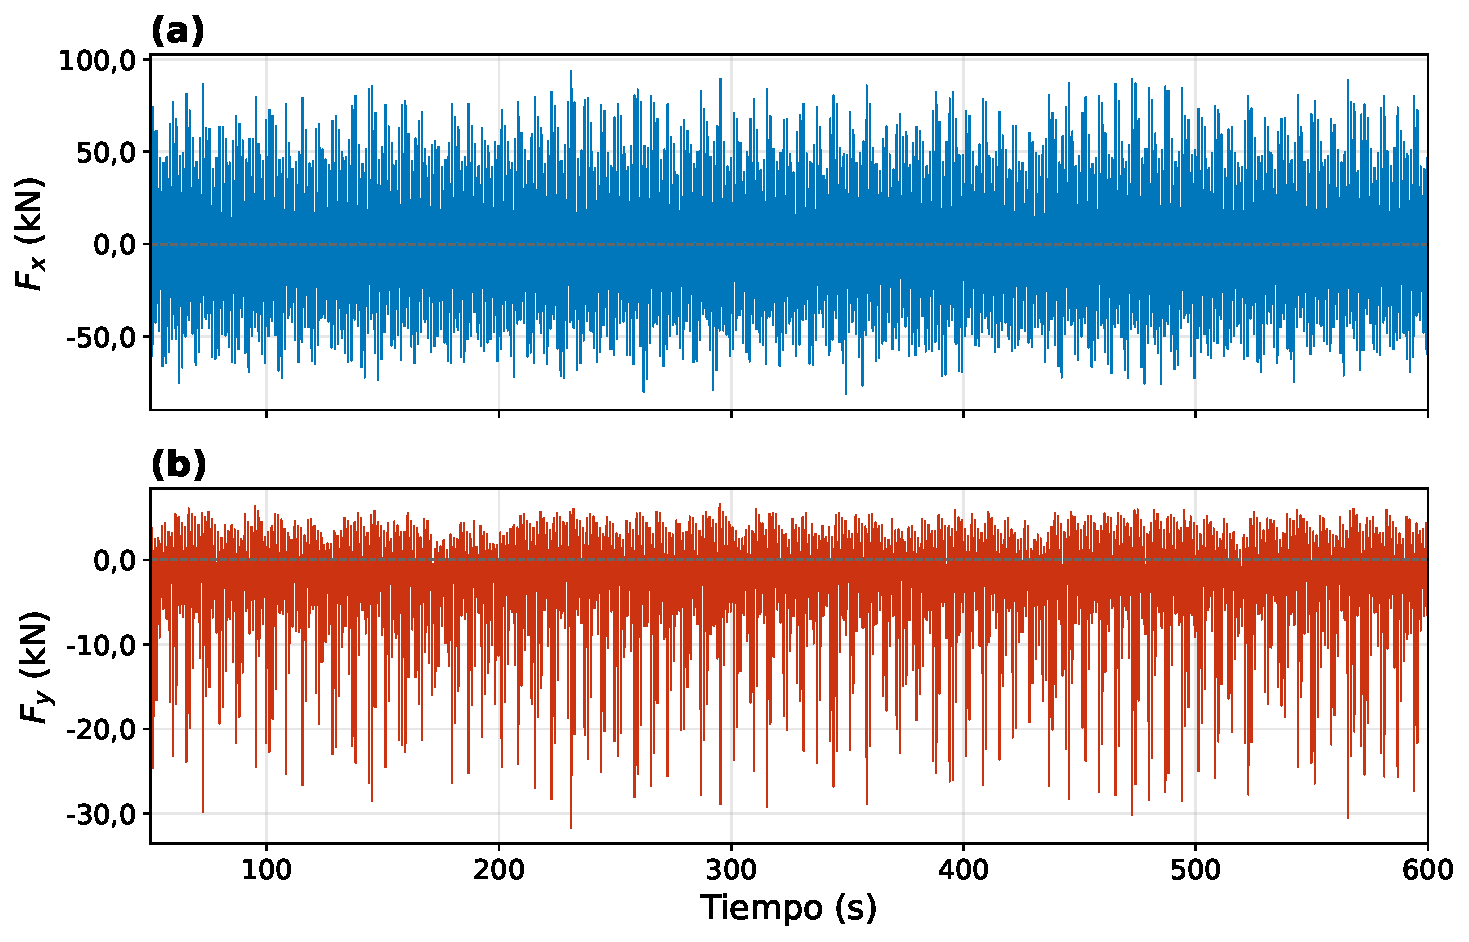
\includegraphics[width=0.85\textwidth]{Figuras/Figuras Anexo Fuerzas/fuerzas_xy_V24_S5.pdf}
    \caption{Fuerzas resultantes (a) $F_x$ y (b) $F_y$ en función del tiempo, $V = 24$~m/s, semilla $5$.}
    \label{fig:anexo_fuerzas_xy_V24_S5}
\end{figure}

\begin{figure}[H]
    \centering
    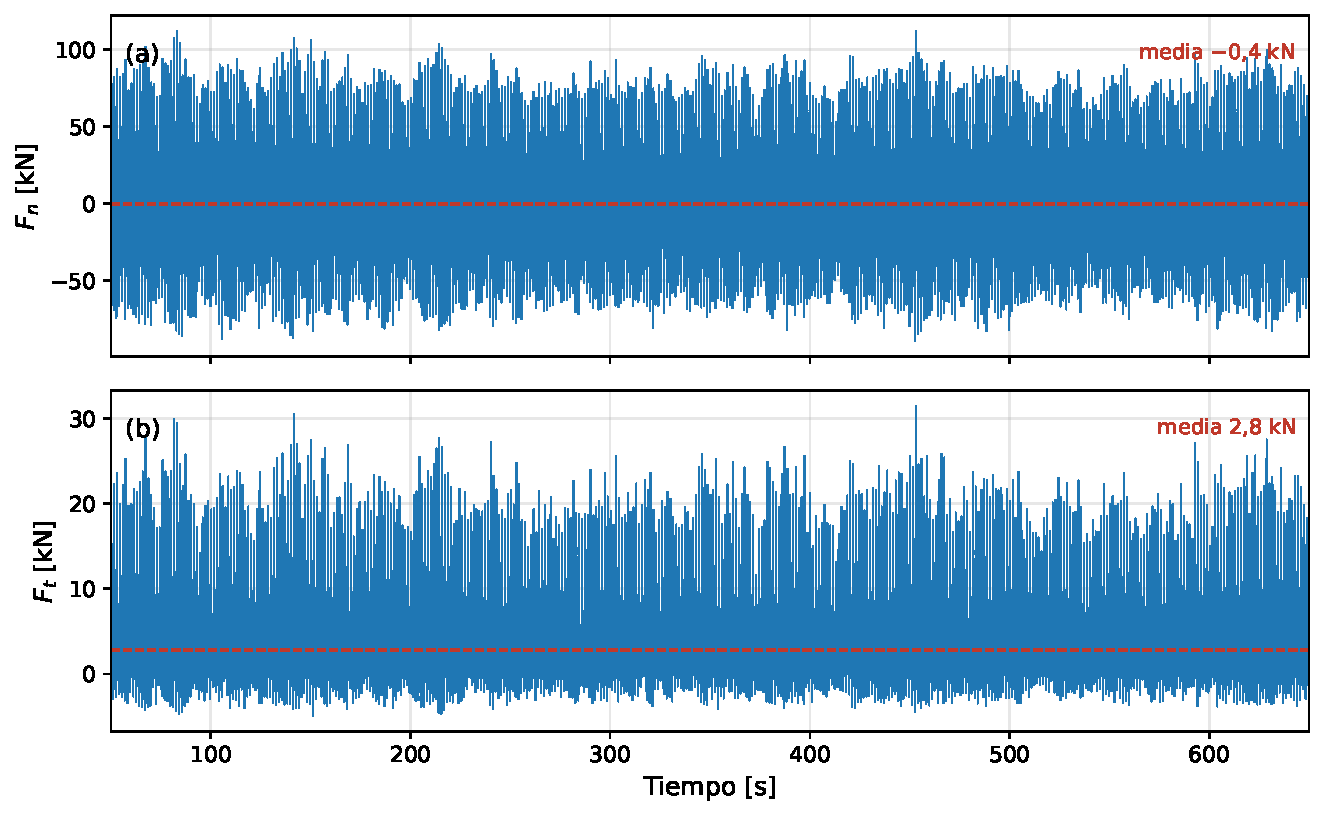
\includegraphics[width=0.85\textwidth]{Figuras/Figuras Anexo Fuerzas/fuerzas_xy_V24_S6.pdf}
    \caption{Fuerzas resultantes (a) $F_x$ y (b) $F_y$ en función del tiempo, $V = 24$~m/s, semilla $6$.}
    \label{fig:anexo_fuerzas_xy_V24_S6}
\end{figure}


\end{document}